\documentclass[12pt]{article}
%\usepackage{newlistok}
\usepackage[T1,T2A]{fontenc} %
%\usepackage[cp866]{inputenc} %
\usepackage[cp1251]{inputenc} %
\usepackage[russian]{babel} %
\usepackage{amsmath} %
\usepackage{amssymb}
\usepackage{pgfplots}
\graphicspath{{pictures/}}
\DeclareGraphicsExtensions{.pdf,.png,.jpg}
\pgfplotsset{compat=1.9}
\usepackage{tikz}
\textheight=257mm %
\textwidth =180mm
%\usepackage[active]{srcltx} %
\mathsurround=2pt %
%\textheight=185mm \textwidth =120mm %
\textheight=257mm %
\textwidth =190mm %
\hoffset=-18mm %
\voffset=-41mm
\author{Л.С.Михлин}
\title{Пособие для поступающих в 8---10 классы физико--математических школ}
\date{2020 --- ...}
\begin{document}
\maketitle
\newpage
\tableofcontents
\newpage
\section{Числовые выражения задачи}
1.\ $\left(\cfrac{4}{3}\sqrt{3}+\sqrt{2}+\sqrt{3\frac{1}{3}}\right): \left(-\sqrt{\frac{1}{3}}\right)+\sqrt{2}(\sqrt{3}+\sqrt{5})+\cfrac{9-2\sqrt{3}}{3\sqrt{6}-2\sqrt{2}},$\\
2.\ $\left(\cfrac{1}{4}+\sqrt{\frac{1}{5}}-2\sqrt{2}\right): \left(\cfrac{1}{2}\sqrt{\frac{1}{5}}\right)-\cfrac{1}{2}\sqrt{5}+4\sqrt{10}+\cfrac{2\sqrt{6}+3\sqrt{3}}{4+3\sqrt{2}},$\\
$\begin{array}{ll}
3.\ \sqrt{9+4\sqrt{5}}-\sqrt{6-2\sqrt{5}},&
4.\ \sqrt{12+6\sqrt{3}}-\sqrt{4-2\sqrt{3}},\\
5.\ 2\sqrt{8\frac{1}{2}}-\sqrt{306}+5\sqrt{1\frac{9}{25}},&
6.\ 4\sqrt{10\frac{1}{2}}+\sqrt{168}-15\sqrt{1\frac{17}{25}},\\
7.\ \sqrt{7+4\sqrt{3}}+\sqrt{7-4\sqrt{3}},&
8.\ \sqrt{8+2\sqrt{7}}+\sqrt{8-2\sqrt{7}},\\
9.\ \cfrac{1}{\sqrt{6-\sqrt{20}}+1}-\cfrac{1}{\sqrt{6+\sqrt{20}}-1},&
10.\ \cfrac{1}{\sqrt{4-\sqrt{12}}+1}-\cfrac{1}{\sqrt{4+\sqrt{12}}-1},\\
11.\ \cfrac{\left(\cfrac{1}{4}-\cfrac{5}{24}\right)\cdot 8-\cfrac{1}{3}}{1,85-1,62:0,9},&
12.\ \cfrac{\left(1\cfrac{2}{9}:7\cfrac{1}{3}-\cfrac{1}{6}\right)\cdot0,23}{2\cfrac{1}{8}+\cfrac{1}{2}},\\
13.\ \sqrt{28-10\sqrt{3}}+\sqrt{28+10\sqrt{3}},&
14.\ \sqrt{14+6\sqrt{5}}+\sqrt{14-6\sqrt{5}},\\
15.\ 3458\cfrac{239}{9876}\cdot3457\cfrac{239}{9876}-3459\cfrac{239}{9876}\cdot3456\cfrac{239}{9876},\\
16.\ 4359\cfrac{239}{9876}\cdot4356\cfrac{239}{9876}-4358\cfrac{239}{9876}\cdot4357\cfrac{239}{9876},\\
17.\ \sqrt{6+2\sqrt{5}}-\sqrt{6-2\sqrt{5}},&
18.\ \sqrt{7+2\sqrt{6}}-\sqrt{7-2\sqrt{6}},\\
\end{array}$\\
19. Сравнить числа $a=\sqrt{7-3\sqrt{5}}$ и $b=\cfrac{2}{\sqrt{7+3\sqrt{5}}},$\\
20. Сравнить числа $a=\sqrt{8-2\sqrt{15}}$ и $b=\cfrac{2}{\sqrt{8+2\sqrt{15}}},$\\
$\begin{array}{ll}
21.\ \cfrac{\sqrt{2+\sqrt{3}}-\sqrt{2-\sqrt{3}}}{\sqrt{2}},&
22.\ \cfrac{\sqrt{3+\sqrt{5}}-\sqrt{3-\sqrt{5}}}{\sqrt{2}},\\
23.\ 131\cdot139-133\cdot137,&
24.\ 141\cdot149-143\cdot147,\\
25.\ \sqrt{4+2\sqrt{3}}-\sqrt{4-2\sqrt{3}},&
26.\ \sqrt{16+2\sqrt{15}}-\sqrt{16-2\sqrt{15}},\\
27.\ 5379^2-5378\cdot 5380,&
28.\ 9552\cdot9550-9551^2,\end{array}$\\ $\begin{array}{llll}
29.\ \sqrt{27+10\sqrt{2}}-\sqrt{2},&
30.\ \sqrt{21-8\sqrt{5}}+\sqrt{5},\\
31.\ \cfrac{5,1}{0,017}+\cfrac{0,09}{0,003}+\cfrac{1}{0,1},&
32.\ \cfrac{2,4}{0,08}+\cfrac{0,21}{0,07}+\cfrac{4}{0,4},\\
33.\ \text{Сравнить числа } a=4+2\sqrt{2},\ b=\sqrt{11}+\sqrt{13},\\
34.\ \text{Сравнить числа } a=3+2\sqrt{5},\ b=\sqrt{14}+\sqrt{15},\\
35.\ \cfrac{\sqrt{52}}{\sqrt{\sqrt{17}+2}\sqrt{\sqrt{17}-2}},&
36.\ 562\cdot570-568\cdot564,\\
37.\ \cfrac{15^{n+4}}{3^{n+2}\cdot5^{n+3}},&
38.\ \sqrt{3}\cdot\sqrt{24}\cdot\cfrac{\sqrt{63\cdot16-72\cdot6}}{\sqrt{19^2-17^2}},\\
39.\ \sqrt{2}\cdot\sqrt{18}\cdot\cfrac{\sqrt{36\cdot92-48\cdot9}}{\sqrt{21^2-19^2}},&
40.\ \sqrt{7}\cdot\sqrt{28}\cdot\cfrac{\sqrt{225\cdot32-72\cdot16}}{\sqrt{23^2-19^2}},\\
41.\ \sqrt{5}\cdot\sqrt{45}\cdot\cfrac{\sqrt{126\cdot32+48\cdot18}}{\sqrt{19^2-15^2}},&
42.\ \sqrt{1-2\sqrt{3}+3}+\sqrt{3},\\
43.\ -\sqrt{5}-\sqrt{1-2\sqrt{5}+5},&
44.\ -\sqrt{3}-\sqrt{1-2\sqrt{3}+3},\\
45.\ \sqrt{5}+\sqrt{1-2\sqrt{5}+5},&
46.\ \sqrt{83-18\sqrt{2}}-\sqrt{2},\\
47.\ \sqrt{54-14\sqrt{5}}+\sqrt{5},&
48.\ (2-\sqrt{5})(\sqrt{9+4\sqrt{5}}),\\
49.\ (2-\sqrt{7})(\sqrt{11+4\sqrt{7}}),
\end{array}$\\$\begin{array}{ll}
50.\ \cfrac{180\cdot3,91-168+859\cdot1,8-768}{239\cfrac{5}{6}-237\cfrac{2}{3}},&
51.\ \cfrac{1,7\cdot229-1155+7,91\cdot170+937}{366\cfrac{5}{6}-364\cfrac{29}{42}},\\
52.\ \cfrac{(8^{2020}+8^{2019})^2}{(4^{2019}-4^{2018})^3},&
53.\ \cfrac{(4^{3021}-4^{3020})^3}{(8^{3020}+8^{3019})^2},\\
54.\ \left(30\cfrac{1}{239}\right)^2-31\cfrac{1}{239}\cdot29\cfrac{1}{239},&
55.\ (2-\sqrt{5})\sqrt{18+8\sqrt{5}},\\
56.\ \cfrac{1}{\sqrt{7+4\sqrt{3}}}+\cfrac{1}{\sqrt{7-4\sqrt{3}}},&
57.\ \cfrac{1}{\sqrt{9+4\sqrt{5}}}+\cfrac{1}{\sqrt{9-4\sqrt{5}}},
\end{array}$\\
58. Сравните числа $\cfrac{1}{\sqrt{3}-\sqrt{2}}$ и $2\sqrt{2},$\\
59. Сравните числа $\sqrt{10}+\sqrt{13}$ и $\sqrt{12}+\sqrt{11},$\\
60. Сравните числа $\cfrac{1}{2+\sqrt{17-12\sqrt{2}}}$ и $\cfrac{8}{17},$\\
$\begin{array}{lll}
61.\ (4+\sqrt{15})(\sqrt{10}-\sqrt{6})\sqrt{4-\sqrt{15}},&
62.\ \cfrac{3^2-0,363^2}{3,363},&
63.\ \cfrac{\left(0,875-\cfrac{1}{8}\right):0,75-1}{0,125+\cfrac{7}{8}},\\
64.\ \left(\sqrt{3+\sqrt{5}}+\sqrt{3-\sqrt{5}}\right)^2,
\end{array}$\\
$\begin{array}{ll}
65.\ \sqrt{\sqrt{2016\cdot2018\cdot2020\cdot2022+16}+5},&
66.\ \sqrt{\sqrt{2013\cdot2015\cdot2019\cdot2021+36}+10},\\
67.\ \left(\cfrac{1}{2+\sqrt{3}}-\cfrac{1}{2-\sqrt{3}}\right)(\sqrt{12}-\sqrt{75}),&
68.\ \left(\cfrac{1}{3+\sqrt{5}}-\cfrac{1}{3-\sqrt{5}}\right)(\sqrt{5}+\sqrt{45}),\\
69.\ \sqrt{(\sqrt{2}-3)^2}+\sqrt{27+10\sqrt{2}},&
70.\ \cfrac{\left(0,5:1,25+\cfrac{7}{5}:1\cfrac{4}{7}-\cfrac{3}{11}\right)\cdot3}{\left(1,5+\cfrac{1}{4}\right):18\cfrac{1}{3}},\\
71.\ \left(\cfrac{(2,7-0,8)\cdot2\cfrac{1}{3}}{(5,2-1,4):\cfrac{3}{70}}+0,125\right):2\cfrac{1}{2}+0,43,\\
72.\ \left(\cfrac{1}{2}\sqrt{6}-3\sqrt{3}+5\sqrt{2}-\sqrt{8}\right)\cdot\sqrt{24}+18\sqrt{2}-12\sqrt{3},\\
73.\ \left(\cfrac{1}{2}\sqrt{32}-\cfrac{1}{3}\sqrt{3}+4\sqrt{15}-\sqrt{8}\right)\cdot\sqrt{12}-4\sqrt{6}-24\sqrt{5},&
74.\ \sqrt{7+4\sqrt{3}}+\sqrt{7-4\sqrt{3}},\\
75.\ \sqrt{8+2\sqrt{7}}-\sqrt{8-2\sqrt{7}},&
76.\ 2\sqrt{9\cfrac{1}{2}}-\sqrt{342}+5\sqrt{1\cfrac{13}{25}},\\
77.\ \cfrac{2^{19}\cdot27^3+15\cdot4^9\cdot9^4}{6^9\cdot2^{10}+12^{10}},&
78.\ \cfrac{4^{15}\cdot9^9-4\cdot3^{20}\cdot8^9}{2^9\cdot6^{19}-5\cdot2^{29}\cdot27^6},\end{array}$\\
79. $\left(\cfrac{1}{2}\sqrt{6}-\sqrt{12}+0,5\sqrt{24}+\cfrac{3\sqrt{48}}{4}\right)\cdot2\sqrt{2},$\qquad
80. $(8\sqrt{24}-12\sqrt{54}+6\sqrt{96}-4\sqrt{150}):2\sqrt{3}.$\\
81. Лежит ли в промежутке $(3;4)$ число $\sqrt{5-\sqrt{24}}+\sqrt{5+\sqrt{24}}?$\\
$\begin{array}{ll}
82.\ \cfrac{17\sqrt{3}}{3\sqrt{5}-7\sqrt{3}}-\cfrac{3\sqrt{5}-\sqrt{3}}{5\sqrt{3}-4\sqrt{5}},&
83.\ \cfrac{2\sqrt{5}-\sqrt{3}}{5\sqrt{3}-4\sqrt{5}}-\cfrac{21\sqrt{5}}{4\sqrt{5}-6\sqrt{3}},
\end{array}$\\
84. Сравните $(\sqrt{10}-\sqrt{5})\cdot\sqrt{\cfrac{20}{(1-\sqrt{2})^2}}$ и 9,99.\\
85. Сравните $(\sqrt{8}+\sqrt{10})\cdot\sqrt{32\cdot(2-\sqrt{5})^2}$ и 7,99.\\
86. Найдите число, $36\cfrac{2}{3}\%$ от которого составляют
$\cfrac{\left(5\cfrac{7}{30}-3\cfrac{5}{18}\right):2\cfrac{2}{3}}{(1,2)^2-1,26:0,9}.$\\
87. $\cfrac{18^{n+3}}{3^{2n+5}\cdot2^{n+2}},$ \quad 88. $\left(\cfrac{76^2+44^2+2\cdot44\cdot76}{120}\right):(37^2-13^2),$\quad
89. $4322^2-4321\cdot4323,$ \\ 90. $\sqrt{9-4\sqrt{5}}-\cfrac{4}{\sqrt{5}+1},$ \qquad \qquad
91. Что больше: $\sqrt{48}+\sqrt{11}$ или $\sqrt{27}+5?$ \\
92. Что больше: $\sqrt{8}+5$ или $\sqrt{18}+\sqrt{13}?$\\
$\begin{array}{ll}
93.\ \sqrt{(2\sqrt{2}-3)^2}-\cfrac{8}{4+2\sqrt{2}},&
94.\ \sqrt{(\sqrt{17}-3\sqrt{2})^2}+\cfrac{1}{\sqrt{17}-4}-3\sqrt{2}.
\end{array}$
\newpage
\section{Преобразование буквенных выражений задачи}
1. Упростить выражение $\sqrt{4x^2-4x+1}+\sqrt{16x^2-8x+1}$ при $\cfrac{1}{4}\leqslant x\leqslant\cfrac{1}{2},$\\
2. Упростить выражение $\sqrt{25x^2+10x+1}+\sqrt{9x^2+6x+1}$ при $-\cfrac{1}{3}\leqslant x\leqslant-\cfrac{1}{5}.$\\
3.\ $\cfrac{(5a-4)^2+2(5a-4)(4-3a)+(3a-4)^2}{(2a+5)^2-2(2a+5)(5-3a)+(3a-5)^2},$\\
4.\ $\cfrac{(4b-5)^2+2(4b-5)(5-b)+(b-5)^2}{(7b+4)^2-2(7b+4)(4-3b)+(3b-4)^2},$\\
$\begin{array}{ll}
5.\ \cfrac{a-b}{a-3\sqrt{ab}+2b}\ (a\geqslant0,\ b\geqslant0),&
6.\ \cfrac{x+4\sqrt{xy}+3y}{x-y}\ (x\geqslant0,\ y\geqslant0),\\
7.\ \cfrac{x^4-2x^3+x-2}{x^3-3x^2+3x-2},&
8.\ \cfrac{x^6+x^4-x^2-1}{x^3+x^2+x+1},\\
9.\ \left(\cfrac{\sqrt{a}+1}{\sqrt{a}-1}-\cfrac{\sqrt{a}-1}{\sqrt{a}+1}+4\sqrt{a}\right)\cdot
\left(\sqrt{\cfrac{a}{4}}-\sqrt{\cfrac{1}{4a}}\right),\\
10.\ \left(\cfrac{\sqrt{a}}{\sqrt{a}+\sqrt{b}}+\cfrac{\sqrt{b}}{\sqrt{a}-\sqrt{b}}+
\cfrac{2\sqrt{ab}}{a-b}\right)\cdot\left(\sqrt{a}-\cfrac{\sqrt{ab}+b}{\sqrt{a}+\sqrt{b}}\right),
\end{array}$\\
$\begin{array}{ll}
11.\ a^3-7a+6,&
12.\ a^3-7a-6,\\
13.\ \cfrac{a^4+4}{(a+1)^2+1},&
14.\ \cfrac{b^4+64}{(b-2)^2+4},\end{array}$\\ $\begin{array}{ll}
15.\ \left(\sqrt{a}+\cfrac{b}{\sqrt{a}-\sqrt{b}}\right)\cdot\left(1-\cfrac{\sqrt{b^3}}{a\sqrt{a}+b\sqrt{b}}\right)\cdot
(\sqrt{a}+\sqrt{b}),\\
16.\ \left(\sqrt{a}+\cfrac{b}{\sqrt{a}+\sqrt{b}}\right)\cdot\left(1+\cfrac{\sqrt{b^3}}{a\sqrt{a}-b\sqrt{b}}\right)\cdot
(\sqrt{a}-\sqrt{b}),\\
17.\ \cfrac{a+1}{a^4+a^3+a^2}: \cfrac{1}{a^5-a^2},&
18.\ \cfrac{a-1}{a^4-a^3+a^2}: \cfrac{1}{a^5+a^2},\\
19.\ a^3+2a-3,&
20.\ a^3+3a-4,
\end{array}$\\
$\begin{array}{ll}
21.\ \cfrac{m\sqrt{m}-\sqrt{125}}{\sqrt{m}-\sqrt{5}}\cdot\cfrac{1}{m-5}-\cfrac{2\sqrt{5}}{\sqrt{m}-\sqrt{5}}+\cfrac{\sqrt{5m}}{m-5}.\\
\end{array}$\\
$\begin{array}{llll}
22.\ \cfrac{a\sqrt{a}+27}{a-3\sqrt{a}+9}-3,&
23.\ \cfrac{a\sqrt{a}-27}{a+3\sqrt{a}+9}+3,&
24.\ 2a^3+3a^2-5,&
25.\ 2a^3+3a-5,\\
26.\ \cfrac{\cfrac{1}{a+b}-\cfrac{1}{a-b}}{\cfrac{1}{a+b}+\cfrac{1}{a-b}}\cdot\cfrac{a}{b},&
27.\ \cfrac{\cfrac{1}{a-b}-\cfrac{1}{a+b}}{\cfrac{1}{a-b}+\cfrac{1}{a+b}}\cdot\cfrac{a}{b},&
28.\ \cfrac{x^4+4}{(x+1)^2+1},&
29.\ \cfrac{x^4+4}{(x-1)^2+1},\\
30.\ \sqrt{b-2+2\sqrt{b-3}},&
31.\ \sqrt{a-1+2\sqrt{a-2}},
\end{array}$\\
32. $\cfrac{a^2}{(a+1)(a-c)}+\cfrac{1}{(c+1)(a+1)}+\cfrac{c^2}{(c-a)(c+1)},$\\
33. $\cfrac{9}{(b-3)(c-3)}-\cfrac{b^2}{(b-c)(3-b)}-\cfrac{c^2}{(3-c)(c-b)},$\\
$\begin{array}{llll}
34.\ \cfrac{a^2-4b^2}{0,5a-b}-4b,&
35.\ \cfrac{4a^2-b^2}{a-0,5b}-4a,&
36.\ a^3-2a+1,&
37.\ a^3-2a-1,\end{array}$\\ $\begin{array}{lll}
38.\ \cfrac{x}{a}-\cfrac{x^2-a^2}{a^2}\cdot\cfrac{a}{x+a},&
39.\ \cfrac{b^2-c^2}{c^2}\cdot\cfrac{c}{b-c}-\cfrac{b}{c},&
40.\ 3x^2-11xy-4y^2,\\
41.\ 6y^2+11xy-2x^2,&
42.\ \cfrac{x^3+5x^2+3x-9}{x^2+6x+9},&
43.\ \cfrac{x^3-2x^2-5x+6}{x^2-4x+3},\\
44.\ \cfrac{a\sqrt{a}-1}{a+\sqrt{a}-2}+\cfrac{3(\sqrt{a}+1)}{\sqrt{a}+2},&
45.\ \cfrac{a\sqrt{a}+1}{a-\sqrt{a}-2}-\cfrac{3(\sqrt{a}-1)}{\sqrt{a}-2},
\end{array}$\\
46. Вычислить $\sqrt{t^2+\cfrac{9}{t^2}+6}$ при $t=-0,5.$\\
47. Вычислить $\sqrt{t^2+\cfrac{4}{t^2}+4}$ при $t=-0,5.$\\
48. $\left(\sqrt{m}+\cfrac{n}{\sqrt{m}+\sqrt{n}}\right)\left(1+\cfrac{\sqrt{n^3}}{m\sqrt{m}-n\sqrt{n}}\right)(
\sqrt{m}-\sqrt{n}),$\\
$\begin{array}{llll}
49.\ a^2-9b^2+12bc-4c^2,&
50.\ a^2-4b^2+12bc-9c^2,&
51.\ \cfrac{2\sqrt{x}+x-x\sqrt{x}}{x-2\sqrt{x}},\\
52.\ \cfrac{3\sqrt{x}-2x-x\sqrt{x}}{x+3\sqrt{x}},&
53.\ x^3+4x^2+x-6,&
54.\ x^3-4x^2+x+6,\end{array}$\\ $\begin{array}{ll}
55.\ \left(c-\cfrac{c^3+8}{2c+c^2}\right)\cdot\cfrac{c}{c^2-4c+4}+\cfrac{2}{2-c},&
56.\ \left(c+\cfrac{8-c^3}{c^2-2c}\right)\cdot\cfrac{c}{c^2+4c+4}+\cfrac{2}{2+c},\\
57.\ 9-x(x-y-3)+3(x-3-y)-y(3+y-x),\\
58.\ 4-2(2-b-a)+a(2-a-b)-b(a+b-2),\\
59.\ \cfrac{x\sqrt{x}-y\sqrt{y}}{\sqrt{x}-\sqrt{y}},&
60.\ \cfrac{x\sqrt{x}+y\sqrt{y}}{\sqrt{x}+\sqrt{y}},\\
61.\ \cfrac{a^2-1}{3a^2-4a+1}\cdot\cfrac{3a-1}{a}-\cfrac{1}{a},&
62.\ \cfrac{a^2-1}{4a^2-5a+1}\cdot\cfrac{4a-1}{a}-\cfrac{1}{a},
\end{array}$\\
63. Упростите $\sqrt{xy}\left(\cfrac{x}{y}\sqrt{xy}-2\sqrt{\frac{x}{y}}+\sqrt{\frac{1}{xy}}\right),$ где $x>0,\ y>0,$\\
$\begin{array}{llll}
64.\ \cfrac{36+x}{6-\sqrt{-x}},&
65.\ \cfrac{49x+1}{1+7\sqrt{-x}},&
66.\ 1+4a^2b^2-(a^2+b^2)^2,&
67.\ 4x^2y^2-(x^2+y^2)^2+1,
\end{array}$\\
$\begin{array}{llll}
68.\ \left(\sqrt{ab}+\cfrac{a\sqrt{a}-b\sqrt{b}}{\sqrt{a}-\sqrt{b}}\right)\cdot\cfrac{a-\sqrt{ab}}{
a\sqrt{a}-b\sqrt{a}},&
69.\ \left(\cfrac{x\sqrt{x}-8}{x-3\sqrt{x}+2}-\cfrac{6\sqrt{x}}{\sqrt{x}-1}\right):
\left(1-\cfrac{1}{\sqrt{x}-1}\right),\\
70.\ \left(\cfrac{1-x\sqrt{x}}{1+x+\sqrt{x}}+\sqrt{x}\right): \cfrac{1+\sqrt{x}}{1-x},&
71.\ \left(\cfrac{a^3-8}{a^2-4}-\cfrac{6a}{a+2}\right): \left(1-\cfrac{4}{a+2}\right)^2,\\
72.\ \cfrac{b^2-1}{3b^2-4b+1}\cdot\cfrac{3b-1}{b}-\cfrac{1}{b},&
73.\ \cfrac{\sqrt{-ab^2}-\sqrt{a^2b}}{ab}-\cfrac{1}{\sqrt{b}},\\
74.\ \cfrac{\sqrt{x}+1}{x\sqrt{x}+x+\sqrt{x}}:\cfrac{1}{x^2-\sqrt{x}},\end{array}$\\
75. $\cfrac{1}{x^2}\cdot\left(\cfrac{1}{(x-y)^2}+\cfrac{1}{y^2}\right)+\cfrac{2}{x^3}\cdot\left(
\cfrac{1}{x-y}+\cfrac{1}{y}\right)-\cfrac{1}{(x-y)^2y^2}.$\\
76. $\left(\sqrt{\sqrt{7}-\sqrt{5-a}}\right)\cdot\sqrt{2+a}\cdot\left(\sqrt{\sqrt{7}+\sqrt{5-a}}\right)-a,$\\
77. $\left(\sqrt{\sqrt{5}-\sqrt{3-a}}\right)\cdot\sqrt{2+a}\cdot\left(\sqrt{\sqrt{5}+\sqrt{3-a}}\right)-a,$\\
78. Упростите выражение $\sqrt{a^2-4a+4}+\sqrt{a^2-12a+36}$ и найдите его значение\\
а) при $a=-\cfrac{2}{7};$ б) при $a=\sqrt{3+\sqrt{2}}.$\\
79. Упростите выражение $\sqrt{a^2-2a+1}+\sqrt{a^2-8a+16}$ и найдите его значение\\
а) при $a=\cfrac{2}{7};$ б) при $a=\sqrt{3-\sqrt{2}}.$\\
80. $x^4+64,$ \qquad \qquad 81. $\left(\cfrac{a\sqrt{a}+b\sqrt{b}}{\sqrt{a}+\sqrt{b}}-\sqrt{ab}\right):(a-b)+\cfrac{2\sqrt{b}}{\sqrt{a}+\sqrt{b}},$\\
82. $36a^2-b^2+24bc-144c^2,$ \qquad \qquad 83. $49m^2-121n^2+22nk-k^2,$\\
84. $\cfrac{6y-x}{x-2y}:\left(\cfrac{1}{x-2y}+\cfrac{1}{x-3y}-\cfrac{x+y}{x^2-5xy+6y^2}\right),$
85. $\cfrac{3y-2x}{2x+y}:\left(\cfrac{1}{2x+y}-\cfrac{1}{3x-y}+\cfrac{x-y}{6x^2+xy-y^2}\right),$\\
86. $\left(\cfrac{\sqrt{b}}{\sqrt{a}-\sqrt{b}}-\cfrac{\sqrt{b}}{\sqrt{a}+\sqrt{b}}\right)\cdot\cfrac{\sqrt{a}+\sqrt{b}}{2b},$\qquad\qquad
87. $\left(\cfrac{\sqrt{a}}{\sqrt{a}-\sqrt{b}}+\cfrac{\sqrt{a}}{\sqrt{a}+\sqrt{b}}\right)\cdot\cfrac{\sqrt{a}-\sqrt{b}}{2a},$\\
88. $x^2+2xy+y^2-z^2,$\\
89. Представить в виде степени $\cfrac{2^{n+2}+2^{n+2}}{3^{n+3}},$\\
90. $\left(\cfrac{\sqrt{a}}{\sqrt{a}+\sqrt{b}}+\cfrac{\sqrt{b}}{\sqrt{a}-\sqrt{b}}+\cfrac{2\sqrt{ab}}{a-b}\right)\left(\sqrt{a}-\cfrac{\sqrt{ab}+b}{\sqrt{a}+\sqrt{b}}\right),$
\qquad 91. $a^3+a^2+2a-4,$\\
92. $\left(\cfrac{d-2}{d+2}-\cfrac{d^3+8}{d^2-4d+4}\cdot\cfrac{2-d}{d^2-2d+4}\right):\left(d+2+\cfrac{8}{d-2}\right),$\\
93. $\left(\cfrac{c+2}{c-2}-\cfrac{8-c^3}{c^2+4c+4}\cdot\cfrac{c+2}{c^2+2c+4}\right):\left(c-2+\cfrac{8}{c+2}\right),$\\
94. а) Упростите $T=\left(\cfrac{4}{2\sqrt{a}-3\sqrt{b}}-\cfrac{14\sqrt{b}}{2a+\sqrt{ab}-6b}+\cfrac{7}{\sqrt{a}+2\sqrt{b}}\right):\left(\cfrac{1}{\sqrt{a}+2\sqrt{b}}-\cfrac{1}{\sqrt{a}}\right).$\\
б) Найдите значение $T$ при $a=92,\ b=207.$\\
в) Найдите значение $T$ при $a=153,\ b=68.$\\
95. а) Упростите $M=\left(\cfrac{1}{\sqrt{c}+3\sqrt{d}}-\cfrac{1}{\sqrt{c}}\right):\left(\cfrac{6}{3\sqrt{c}-2\sqrt{d}}-\cfrac{22\sqrt{d}}{3c+7\sqrt{cd}-6d}+\cfrac{3}{\sqrt{c}+3\sqrt{d}}\right).$\\
б) Найдите значение $M$ при $c=99,\ d=275.$\\
в) Найдите значение $M$ при $c=76,\ d=171.$\\
$\begin{array}{ll}
96.\ \cfrac{x^2+x\sqrt{2}}{x^2+2}\left(\cfrac{x}{x-\sqrt{2}}-\cfrac{\sqrt{2}}{x+\sqrt{2}}\right),&
97.\ \left(\cfrac{\sqrt{a}}{\sqrt{a}-\sqrt{b}}-\cfrac{\sqrt{b}}{\sqrt{a}+\sqrt{b}}\right)\cdot\cfrac{a-b}{a^2+ab},\\
98.\ \left(\cfrac{\sqrt{a}-5}{\sqrt{a}+5}+\cfrac{20\sqrt{a}}{a-25}\right):\cfrac{\sqrt{a}+5}{a-5\sqrt{a}},&
99.\ \left(\sqrt{ab}+\cfrac{a\sqrt{a}-b\sqrt{b}}{\sqrt{a}-\sqrt{b}}\right)\cdot\cfrac{a-\sqrt{ab}}{a\sqrt{a}-b\sqrt{a}},\\
100.\ \left(1+\cfrac{\sqrt{xy}}{x+y+\sqrt{xy}}\right)\cdot\cfrac{x\sqrt{x}-y\sqrt{y}}{y-x},&
101.\ \left(1-\cfrac{\sqrt{xy}}{x+y-\sqrt{xy}}\right)\cdot\cfrac{x\sqrt{x}+y\sqrt{y}}{y-x},\\
102.\ x^4+2x^3y-3x^2-2x-6xy-4y,&
103.\ x^4-2x^3y-3x^2+6xy+2x-4y,\\
104.\ \left(\cfrac{1}{a+\sqrt{2}}-\cfrac{a^2+4}{a^3+2\sqrt{2}}\right) \left (\cfrac{a-\sqrt{2}}{2}+\cfrac{1}{a}\right),&
105.\ \left(\cfrac{1}{a-\sqrt{3}}-\cfrac{a^2+6}{a^3-3\sqrt{3}}\right) \left (\cfrac{a+\sqrt{3}}{3}+\cfrac{1}{a}\right).
\end{array}$
\newpage
\section{Уравнения задачи}
$\begin{array}{ll}
1.\ \cfrac{3x-2}{x}+\cfrac{1}{2-x}=\cfrac{3x+4}{x^2-2x},&
2.\ \cfrac{1}{3-x}-\cfrac{2x+6}{x^2-3x}=\cfrac{2-5x}{x},\\
3.\ (x+5)^4+8(x+5)^2-9=0,&
4.\ (x-4)^4-3(x-4)^2-4=0,\\
5.\ \cfrac{6x}{x+1}=\cfrac{12x}{x^2-x+1}-\cfrac{12x^2-6x}{x^3+1},&
6.\ \cfrac{5x}{1-x}=\cfrac{10x}{x^2+x+1}+\cfrac{10x^2+5x}{1-x^3},\end{array}$ \\ $\begin{array}{ll}
7.\ \cfrac{3}{1+x+x^2}=3-x-x^2,&
8.\ \cfrac{2}{1+x+x^2}=2-x-x^2,\\
9.\ |x+1|+|x+2|=1,&
10.\ |x-1|+|x-2|=1,\\
11.\ (x+3)^2-|x+3|-30=0,&
12.\ (x-2)^2-3|x-2|-28=0,\end{array}$ \\ $\begin{array}{ll}
13.\ (x-1)^4-x^2+2x-73=0,&
14.\ (x+2)^4+2x^2+8x-16=0,\\
15.\ |x-3|+|x-5|=2,&
16.\ \cfrac{1}{x-5}-\cfrac{3}{x-3}=\cfrac{2}{x-4}-\cfrac{4}{x-2},\end{array}$ \\ $\begin{array}{ll}
17.\ \cfrac{3}{x-2}-\cfrac{4}{x-1}=\cfrac{1}{x-4}-\cfrac{2}{x-3},&
18.\ |3x+8|=x,\\
19.\ |2x+9|=x,&
20.\ \cfrac{1}{x+5}+\cfrac{1}{x+3}+\cfrac{1}{x-5}+\cfrac{1}{x-3}=0,\\
21.\ \cfrac{1}{x+4}+\cfrac{1}{x+2}+\cfrac{1}{x-4}+\cfrac{1}{x-2}=0,&
22.\ (x-1)^4-x^2+2x-13=0,\\
23.\ (x+1)^4-x^2-2x-13=0,&
24.\ |x^2-3x+5|=|4-2x-2x^2|,\\
25.\ \cfrac{2}{x-1}=\cfrac{x+5}{x^2+x-2},&
26.\ \cfrac{2}{x+1}=\cfrac{x-5}{x^2-x-2},\\
27.\ |x|-x+2=|2x-2|,&
28.\ |x|+x+2=|2x+2|,\\
29.\ \cfrac{x}{x-4}-\cfrac{1}{x+1}=\cfrac{2-x}{x+1}+\cfrac{3}{x-4},&
30.\ \cfrac{1}{x-1}+\cfrac{x}{x+4}=\cfrac{2+x}{1-x}-\cfrac{3}{x+4},\\
31.\ |5x-x^2-6|=x^2-5x-6,&
32.\ |5x-x^2-6|=5x-x^2-6,\end{array} \\ \begin{array}{ll}
33.\ \begin{cases}
x+2y=3,\\
x^2+y=2.\end{cases},&
34.\ \begin{cases}
x-2y=3,\\
x^2-y=2.\end{cases},\\
35.\ \cfrac{4x+8}{x^2-4}+2x+5=0,&
36.\ \cfrac{6x-18}{x^2-9}+2x-7=0,\\
37.\ (x^2-x+1)(2x^2-2x+1)=10,&
38.\ (x^2+x+1)(2x^2+2x+1)=10,\\
39.\ |x^2-10|=6,&
40.\ |x^2-17|=8,\\
41.\ \begin{cases}
x^2-16y^2+x+4y=0,\\
3x-4y=16.
\end{cases},&
42.\ \begin{cases}
x^2-9y^2+x-3y=0,\\
4x+3y=10.
\end{cases},\end{array}$\\ $\begin{array}{ll}
43.\ 2x^2+3x-17=2(2-\sqrt{7})^2+3(2-\sqrt{7})-17,&
44.\ x^2+2(1+\sqrt{8})x+8\sqrt{2}=0,\\
45.\ \cfrac{x}{x-2}+\cfrac{5}{x+2}=\cfrac{8}{x^2-4},&
46.\ \cfrac{x}{x+2}-\cfrac{5}{x-2}=\cfrac{8}{x^2-4},\\
47.\ (x+2)^3-x^3=2,&
48.\ (2-x)^3+x^3=2,\\
49.\ \cfrac{36}{4-x^2}+2=\cfrac{1-x}{x+2}-\cfrac{9}{x-2},&
50.\ \cfrac{3x}{x+3}-\cfrac{42}{x^2-9}=1+\cfrac{7}{3-x},\\
51.\ \cfrac{2x+1}{1+x}=\cfrac{2}{x^2-1},&
52.\ \cfrac{1-2x}{x-1}=\cfrac{-2}{x^2-1},\\
53.\ \sqrt{x-3}(3x^2-14x+8)=0,&
54.\ \sqrt{x-2}(3x^2-11x+6)=0,\\
55.\ 2|x+1|=|5-x|,&
56.\ 2|x+2|=|4-x|,\\
57.\ 2|2-x|=|x+7|,&
58.\ 3|3-x|=|x+1|,\\
59.\ \begin{cases}
xy+x^2=10,\\
xy+y^2=15.\end{cases},&
60.\ \begin{cases}
y^2-xy=4,\\
x^2-xy=-3.\end{cases},\\
61.\ (x^2-2x)^2-2x^2+4x=3,&
62.\ (x^2+2x)^2-2x^2-4x=3,\\
63.\ x^3-x^2+4x-4=0,&
64.\ x^3-x^2+5x-5=0,\end{array}\\ \begin{array}{ll}
65.\ \begin{cases}
0,4x+\cfrac{1}{3}y=1,8,\\
\cfrac{1}{5}x+0,27y=1,21.
\end{cases},&
66.\ \begin{cases}
0,4x-\cfrac{1}{3}y=1,8,\\
\cfrac{1}{5}x+0,27y=-0,41.
\end{cases},\\
67.\ |x-7|+|x-5|=x-4,&
68.\ |x-6|+|x-4|=x-3,\\
69.\ (x^2-2x-1)^2+3x^2-6x-13=0,&
70.\ \sqrt{(x-5)^2}=2x-6,\\
71.\ \sqrt{(x-7)^2}=4-3x,&
72.\ \cfrac{-2x^2+3-5x}{x+2}\cdot\sqrt{2-|x|}=0,\\
73.\ \cfrac{4+7x-2x^2}{x-3}\cdot\sqrt{3-|x|}=0,&
74.\ \sqrt{2x-x^2}+\sqrt{x^2-3x+2}+10x=20,\\
75.\ \sqrt{x-2}=100|x-3|+1,&
76.\ x^3+3x^2+3x+\cfrac{7}{8}=0,\\
77.\ 2x^2-3x-4=2(1+\sqrt{2})^2-3(1+\sqrt{2})-4,&
78.\ x^2-2x+1+\sqrt{7x-7}=0,\\
79.\ 2\left||x+4|-1\right|+6=30,&
80.\ (x-2)(x+1)(x+4)(x+7)=63,\end{array}\\ \begin{array}{ll}
81.\ \cfrac{2}{x^2+36+12x}-\cfrac{12}{36-x^2}=\cfrac{1}{x-6},&
82.\ 3x^2+2x+1=3(1-\sqrt{3})^2+2(1-\sqrt{3})+1,\\
83.\ 9x^3+3x^2+3x+1=0,&
84.\ x^3+x^2-4x-4=0,\end{array}\\ \begin{array}{lll}
85.\ |x-7|+|x^2-5|=x-4,&
86.\ 4x^4+3x^2-1=0,&
87.\ \begin{cases}
3x^2-y=7,\\
5y-3x^2=-23.
\end{cases},\\
88.\ x^3+x^2=2x,&
89.\ \begin{cases}
2x^2+xy=40,\\
3x-y=10.
\end{cases},
\end{array}$\\
$\begin{array}{ll}
90.\ \begin{cases}
x-y=3,\\
x^2y-xy^2=-6.
\end{cases},&
91.\ \begin{cases}
y-x=3,\\
x^2y-xy^2=6.
\end{cases},\\
92.\ x^2-6x+7+\cfrac{2}{x^2-6x+10}=0,&
93.\ x^2-3x-1+\cfrac{3}{x^2-3x+3}=0,\\
94.\ |x-1|=2x+1,&
95.\ |x+1|=1-2x,\\
96.\ x^4-3x^2-4=0,&
97.\ x^4+4x^2-5=0, \\
98.\ \cfrac{x+2}{2x-1}+\cfrac{x+1}{x+2}=\cfrac{9x-x^2+2}{2x^2+3x-2},&
99.\ |x^2-4x|=x^2+x-5,\\
100.\ |x^2+4x|=x^2-x-5,&
101.\ \begin{cases} x^2+3xy=1,\\ x-y=1.\end{cases}\\
102.\ \begin{cases} x^2+3xy=1,\\ x+y=1.\end{cases}&
103.\ \cfrac{2}{x-1}+\cfrac{1}{2}=\cfrac{-4}{x^2-4x+3},\\
104.\ \cfrac{1}{x-3}+\cfrac{1}{4}+\cfrac{2}{x^2-8x+15}=0.
\end{array}$\\
105. а) Решите уравнение $x^2-(\sqrt{2}+\sqrt{7})x+\sqrt{14}=0.$\\
б) Какой из корней этого уравнения ближе к числу 2?\\
106. а) Решите уравнение $x^2-(\sqrt{3}+\sqrt{5})x+\sqrt{15}=0.$\\
б) Какой из корней этого уравнения ближе к числу 2?\\
107. Упростить выражение $\left(\cfrac{\sqrt{x}+1}{\sqrt{x}-1}-\cfrac{\sqrt{x}-1}{\sqrt{x}+1}+4\sqrt{x}\right)\cdot\left(\sqrt{x}-\cfrac{1}{\sqrt{x}}\right)$ и определить при каких значениях $x$ это выражение равно выражению $x^2+3.$\\
$\begin{array}{ll}
108.\ (6x-3x^2-2)^5=(2-6x+3x^2)^{10},&
109.\ (x-2)^2-|x-2|-6=0,\\
110.\ x-\sqrt{x+1}-1=0,&
111.\ \cfrac{3}{(x-5)(x+2)}+\cfrac{5}{(x-4)(x+1)}=-2,\\
112.\ \cfrac{10}{(x-3)(x+6)}+\cfrac{9}{(x+4)(x-1)}=-1,&
113.\ |3x^2+18x-23|-|13-2x^2-12x|=-1,\\
114.\ |5x^2-20x-28|-|8x+9-2x^2|=-1,&
115.\ ||x^2-5|-1|=3,\\
116.\ |1-|x^2-6||=2,&
117.\ \left|\cfrac{4}{|x|-2}\right|=x-2,\\
118.\ \left|\cfrac{9}{|x|-3}\right|=x-3,&
119.\ x^2+x+\sqrt{x}-12=\sqrt{x},\\
120.\ 3x^2-2x-5=3(1-\sqrt{2})^2-2(1-\sqrt{2})-5,&
121.\ (x+1)\sqrt{x+3}-1=x,\\
122.\ \cfrac{6x}{x^3+4}+\cfrac{x}{x^3-3}=0,7x,&
123.\ \cfrac{6x}{x^3-4}+\cfrac{x}{x^3+3}=-0,7x,\\
124.\ \begin{cases} x^2+y^2-6x-8y=0,\\ x-4y=3.\end{cases},&
125.\ \begin{cases} x^2+y^2+8x-6y=0,\\ x-5y=-2.\end{cases}.
\end{array}$
\newpage
\section{Неравенства задачи}
$\begin{array}{ll}
1.\ \cfrac{(x^2+5x-14)(x-3)^2}{|x+1|}\leqslant0,&
2.\ \cfrac{(x^2-6x-16)(x+5)^2}{|x-2|}\leqslant0,\\
3.\ \cfrac{(2x^2+7x-4)(x-3)^2}{x+6}\leqslant0,&
4.\ \cfrac{(5x^2+6x+1)(x-2)^2}{x-4}\geqslant0,\\
5.\ \cfrac{(x^2-1)(2x^2-5x-7)}{2-x}\leqslant0,&
6.\ \cfrac{(x^2-1)(2x^2+5x-7)}{3-x}\leqslant0,
\end{array}$\\
7. Доказать неравенство: $a+\cfrac{1}{a}+b+\cfrac{1}{b}\geqslant2\sqrt{ab}+\cfrac{2}{\sqrt{ab}}$ для любых положительных чисел $a$ и $b.$\\
8. Доказать неравенство: $a+b+c\geqslant\sqrt{ab}+\sqrt{bc}+\sqrt{ac}$ для любых положительных чисел $a,\ b,\ c.$\\
9. Доказать, что если $\sqrt{x}-\sqrt{y}=10,$ то $x-2y\leqslant 200.$\\
10. Доказать, что если $\sqrt{x}-\sqrt{y}=8,$ то $x-2y\leqslant128.$\\
$\begin{array}{ll}
11.\ |2x+5|<x+4,&
12.\ |3x+7|<x+3,\\
13.\ \sqrt{x}\cdot|1-x|\cdot(2-x)\cdot(3-x^2)\leqslant0,&
14.\ \sqrt{x}\cdot(1-x)\cdot|2-x|\cdot(3-x)^2\geqslant0,\\
15.\ |x+3|-|2x-4|<5,&
16.\ |x-3|-|2x+4|<5,\\
17.\ \cfrac{x^2+3}{x+1}\leqslant2,&
18.\ \cfrac{x^2}{x-1}\leqslant 4,\\
19.\ |3x-7|+|x+2|>7,&
20.\ \cfrac{\sqrt{x-3}}{(x-1)(x-5)^2(x-6)}\leqslant0,\\
21.\ \cfrac{\sqrt{x-4}}{(x-2)(x-6)^2(x-7)}\leqslant0,&
22.\ |x|\cdot\cfrac{x^3+x^2-x-1}{x^3-x^2-x+1}\geqslant 0,\\
23.\  |x|\cdot\cfrac{x^3-x^2-x+1}{x^3+x^2-x-1}\geqslant 0,&
24.\ |2x-3|<4+x,\\
25.\ |2x-1|<5+x,&
26.\ \cfrac{(x-1)^2(x+3)(x-3)}{\sqrt{x+2}}\geqslant0,\\
27.\ \cfrac{(x-2)^2(x+2)(x-4)}{\sqrt{x+1}}\geqslant0,&
28.\ \cfrac{x^2-3}{x+2}\geqslant-6,\end{array}$\\ $\begin{array}{ll}
29.\ \cfrac{x^2-3}{x-2}\leqslant 6,&
30.\ \cfrac{(x-1)^2(x^2-x-2)}{x^2+3x+2}\geqslant0,\\
31.\ \cfrac{(x+1)^2(x^2+x-2)}{x^2-3x+2}\geqslant0,&
32.\ \cfrac{x^2}{x+2}\leqslant -x,\\
33.\ \cfrac{x^2}{2-x}\leqslant x,&
34.\ |3x+2|\geqslant x^2-2,\\
35.\ |2-3x|\geqslant x^2-2,&
36.\ \cfrac{3}{x}<5,\\
37.\ \cfrac{7}{x}<4,&
38.\ x^2-3x+2>|x-5|,\\
39.\ x^2-5x+6>|x-6|,&
40.\ \cfrac{1}{x-2}+\cfrac{1}{x-1}\geqslant\cfrac{1}{x},\\
41.\ \cfrac{1}{x+2}+\cfrac{1}{x+1}\geqslant\cfrac{1}{x},&
42.\ \cfrac{1}{x-2}+\cfrac{1}{x-3}\geqslant\cfrac{1}{x},\\
43.\ \cfrac{1}{x+2}+\cfrac{1}{x+3}\geqslant\cfrac{1}{x},&
44.\ \left|x^2-6x-7\right|\geqslant-6x+7,\end{array}$ \\ $\begin{array}{ll}
45.\ \left|x^2-2x-15\right|\geqslant-2x+15,&
46.\ \cfrac{x^2-2x-8}{x-4}\leqslant 7,\\
47.\ \cfrac{x^2-4x-5}{x-5}\leqslant 7,&
48.\ \cfrac{7}{(x-1)(x-2)}+\cfrac{9}{x-2}+1\leqslant0,\end{array}$ \\ $\begin{array}{ll}
49.\ \cfrac{1}{3-x}\geqslant\cfrac{1}{(x^2-9)(3-x)},&
50.\ \cfrac{1}{(4-x^2)(x-2)}\leqslant\cfrac{1}{2-x},\\
51.\ \cfrac{x^2-(\sqrt{3}+\sqrt{7})x+\sqrt{21}}{\sqrt{5-x}}\cdot\cfrac{x^2-4x+4}{6x-x^2-9}\leqslant 0,&
52.\ \cfrac{\sqrt{x}}{2x-1}\geqslant\cfrac{\sqrt{x}}{x-5},\\
53.\ x\sqrt{x+2}>x,&
54.\ \cfrac{3x^2+2x^3-x^4}{\sqrt{x+2}}\leqslant0,\\
55.\ x|x-2|\leqslant x-2,&
56.\ -\cfrac{1}{2}x^2+2,5x-3\geqslant0,\\
57.\ \cfrac{4}{x^2-x-6}\geqslant\cfrac{1}{2+x},&
58.\ x^2-x>|x+3|,\\
59.\ \left|x^2-3\right|<\left|3-x\right|,&
60.\ \cfrac{x^2-20}{5x^2+12}\leqslant\cfrac{x-8}{5x^2+12},\\
61.\ \left(1+\left(x-\cfrac{3}{2}\right):3\right)\left(-0,75\right)<0,&
62.\ x^2+x>|x-3|,
\end{array}$\\
63. Найти все значения $x,$ при которых меньшее из чисел $x$ и $x^2-3$ меньше 6.\\
64. Наименьшее из чисел $m,\ n$ обозначается $min(m;n).$ Если числа равны, то тогда\\
$min(m;n)=m=n.$ Найдите все значения $x,$ при которых $min(x+15;x^2+3)\geqslant 4.$\\
65. Найдите все значения $x,$ при которых большее из чисел $x$ и $x^2-3$ не меньше 1.\\
$\begin{array}{lllll}
66.\ \cfrac{2x^3+3x^2}{x-2}\geqslant0,&
67.\ \cfrac{2x^3-3x^2}{x+2}\geqslant0,&
68.\ \cfrac{|3x+2|}{x}<-1,&
69.\ \cfrac{|2x+1|}{x}<-1,\\
70.\ |2x+5|+x<7,&
71.\ \cfrac{x^3+2x^2+7}{7-x}\geqslant1,&
72.\ \cfrac{(x+1)(x-8)^4}{(x+2)^2(5-x)}\geqslant0,&
73.\ \cfrac{x^2(x^2-2x+1)}{(x+7)^3(3-x)}\leqslant0,
\end{array}$\\
74. Найдите наибольшее целое решение неравенства $(2-\sqrt{5})x>2+\sqrt{5}.$\\
75. Найдите наибольшее целое решение неравенства $(\sqrt{3}-2)x>\sqrt{3}+2.$\\
$\begin{array}{lllll}
76.\ |x-3|>6-3x, & 77.\ |x-4|>2x-1, & 78.\ |2x-7|<x, & 79.\ |2x-5|<x,
\end{array}$\\
80. $\cfrac{\sqrt{x+3}(2x^2+13x+15)(x^2+4x-5)(2x+3)}{x^2-1}
\geqslant0,$\\
81. $\cfrac{\sqrt{x+4}(2x^2+13x+20)(x^2+4x-12)(2x+5)}{x^2-4}
\geqslant0,$\\
$\begin{array}{lllll}
82.\ \cfrac{(2x^2+7x-4)(x-3)^2}{x+6}\leqslant0,&
83.\ \cfrac{(2x^2+5x-3)(x-4)^2}{x+5}\leqslant0,\\
84.\ \begin{cases} x^2+3x-4\geqslant0,\\ -x-5<0.\end{cases}&
85.\ \begin{cases} x^2+2x-3\leqslant0,\\ -x-1>0.\end{cases}&
86.\ 2|x-1|\geqslant 2-x,\\
87.\ 2|x+1|\geqslant x+2,\\
88.\ \cfrac{2|x-1|}{2-x}\geqslant1,&
89.\ \cfrac{2|x+1|}{x+2}\geqslant1,&
90.\ \begin{cases} |x^2+2x-15|\leqslant0,\\ x^{15}-3x^{14}+2x-5>0,\end{cases}\\
91.\ -2<\cfrac{1-x}{x}<3,&
92.\ x\cdot|x^2-5x|\leqslant6x,&
93.\ \cfrac{3}{5x-1}+\cfrac{4}{3x+1}\geqslant1,\\
94.\ \cfrac{5}{2x+1}+\cfrac{2}{7x-1}\leqslant3,&
95.\ \cfrac{(x^2-3x+2)(1-x)}{x-3}\geqslant0,&
96.\ \cfrac{3x^3}{x-5}\geqslant\cfrac{-2x^2}{5-x},\\
97.\ |x+2|+|x-2|\leqslant2x,&
98.\ \cfrac{(x-7)\sqrt{x+5}}{x^6-16x^2}\geqslant0,&
99.\ \cfrac{(x-5)\sqrt{x+7}}{x^6-81x^2}\geqslant0,\\
100.\ \cfrac{x^3-9x^2+20x}{x-4}\leqslant0,&
101.\ \cfrac{x^3-8x^2+15x}{x-3}\leqslant0.
\end{array}$
\newpage
\section{Исследование функций и уравнений задачи}
1. В уравнении $x^2-4x+a=0$ сумма квадратов корней уравнения равна 16. Найти $a.$\\
2. В уравнении $x^2-2x+a=0$ квадрат разности корней уравнения равен 16. Найти $a.$\\
3. Найти область определения функции $f(x)=\sqrt{\cfrac{|x-3|(x+4)(x^2+9x+20)}{x^2-x-6}}.$\\
4. Найти область определения функции $f(x)=\sqrt{\cfrac{|x-1|(x+3)(x^2+8x+15)}{x^2+x-2}}.$\\
5. Доказать, что если $c\cdot(a+b+c)<0,$ то квадратный трёхчлен $ax^2+bx+c$ имеет корни.\\
6. Доказать, что если $c\cdot(a-b+c)<0,$ то квадратный трёхчлен $ax^2+bx+c$ имеет корни.\\
7. При каких $k$ уравнение $(k-2)x^2+2(k-1)x+k=0$ имеет единственный корень?\\
8. При каких $k$ уравнение $(k+2)x^2+2(k+1)x+k=0$ имеет единственный корень?\\
9. Найдите наименьшее и наибольшее значение функции на данном промежутке: $y=x^2-7x+6,$ \\
$-1\le x\le 8.$\\
10. Найти область определения функции $y=\sqrt{\cfrac{(x-1)^2(2x-x^2+2)}{(x^2+x-6)|x+2|}}.$\\
11. Найдите наименьшее значение выражения $x^2-2xy+8y^2,$
если $x+2y=4.$\\
12. Найдите наименьшее значение выражения $x^2+2xy+8y^2,$
если $x-2y=4.$\\
13. При каких значениях $a$ уравнение $(x-3)(x-a)(x-2a)=0$ имеет ровно два различных корня?\\
14. При каких значениях $a$ уравнение $(x-5)(x-a)(x-2a)=0$ имеет ровно два различных корня?\\
15. При каких значениях $q$ сумма квадратов корней уравнения $x^2+10x+q=0$ равна 2?\\
16. При каких значениях $q$ сумма квадратов корней уравнения $x^2-10x+q=0$ равна 2?\\
17. Решить относительно $x$ уравнение $(k-1)x^2-(2k-1)x+2=0.$\\
18. Решить относительно $x$ уравнение $(k-1)x^2-(2k-3)x-2=0.$\\
19. Не решая уравнения $2x^2-3x-11=0$ найти $\cfrac{x_1}{x_2}+\cfrac{x_2}{x_1},$ где $x_1,\ x_2$ --- корни этого уравнения.\\
20. Не решая уравнения $2x^2+3x-11=0$ найти $\cfrac{x_1}{x_2}+\cfrac{x_2}{x_1},$ где $x_1,\ x_2$ --- корни этого уравнения.\\
21. Найдите наибольшее значение, которое может принимать $xy,$ если $2x+3y=6.$\\
22. Найдите наибольшее значение, которое может принимать $xy,$ если $3x+2y=6.$\\
23. При каких $k$ один из корней уравнения $x^2-(k+4)x+2k+4=0$ в два раза больше другого?\\
24. При каких $k$ один из корней уравнения $x^2-(k+5)x+2k+6=0$ в два раза больше другого?\\
25. При каких $a$ уравнение $\cfrac{x^2-4ax+3a^2}{x-3}=0$ имеет ровно один корень?\\
26. При каких $a$ уравнение $\cfrac{x^2-5ax+4a^2}{x-4}=0$ имеет ровно один корень?\\
27. Найти те значения $a,$ при которых сумма квадратов корней уравнения $x^2-ax+20=0$ равна 24.\\
28. Найти те значения $b,$ при которых сумма квадратов корней уравнения $x^2-bx+10=0$ равна 16.\\
29. Определить, при каких $x$ и $y$ выражение $5x^2-4x+y^2+2xy+1$ принимает наименьшее значение.\\
30. Определить, при каких $x$ и $y$ выражение $5y^2+4y+x^2-2xy+1$ принимает наименьшее значение.\\
31. При каких значениях $q$ сумма квадратов корней уравнения $x^2-qx+4=0$ равна 17?\\
32. При каких значениях $q$ сумма квадратов корней уравнения $x^2-qx+3=0$ равна 10?\\
33. При каких значениях $t$ уравнение $\cfrac{(x-t)(x-2)}{x-2t}=0$ имеет ровно два разных корня?\\
34. При каких значениях $t$ уравнение $\cfrac{(x-t)(x-4)}{x-4t}=0$ имеет ровно два разных корня?\\
35. При каких значениях $a$ уравнение $(a+1)x^2+2x-a+1=0$ имеет ровно один корень?\\
36. При каких значениях $a$ уравнение $(1-a)x^2-2x+a+1=0$ имеет ровно один корень?\\
37. Вычислить $3x^2-2x-1$ при $x=\cfrac{1-\sqrt{2}}{3}.$\\
38. Вычислить $3x^2+2x-1$ при $x=\cfrac{\sqrt{2}-1}{3}.$\\
39. При каких значениях $x$ выполняется равенство $\sqrt{x^2-4x+3}=\sqrt{1-x}\cdot\sqrt{3-x}?$\\
40. При каких значениях $x$ выполняется равенство $\sqrt{x^2-6x+5}=\sqrt{1-x}\cdot\sqrt{5-x}?$\\
41. Найдите наименьшее значение выражения $2x^2+4xy+4y^2+3.$\\
42. Найдите наименьшее значение выражения $4x^2-4xy+2y^2+5.$\\
43. При каких значениях $t$ неравенство $\cfrac{\sqrt{x-t}}{(x-2)(x-3)}<0$ не имеет корней?\\
44. При каких значениях $t$ неравенство $\cfrac{\sqrt{x-t}}{(x-3)(x-4)}<0$ не имеет корней?\\
45. При каких значениях $a$ уравнение $(a-1)x^2+2ax+4=0$ имеет два различных корня?\\
46. При каких значениях $a$ уравнение $(a+1)x^2-2ax-4=0$ имеет два различных корня?\\
47. Определите, при каких значениях параметра $a$ уравнение $ax^2-(2a+6)x+3a+3=0$ имеет единственное решение.\\
48. Определите, при каких значениях параметра $k$ уравнение $kx^2-2(k+1)x+k+3=0$ имеет единственное решение.\\
49. Пусть $x_1$ и $x_2$ --- корни уравнения $3x^2-5x-11=0.$ Составить квадратное уравнение с корнями $\cfrac{1}{x_1}$ и $\cfrac{1}{x_2}.$\\
50. Пусть $x_1$ и $x_2$ --- корни уравнения $5x^2-3x-11=0.$ Составить квадратное уравнение с корнями $\cfrac{1}{x_1}$ и $\cfrac{1}{x_2}.$\\
51. Найдите произведение вещественных корней уравнения $x^4-3x^2-4=0.$\\
52. Найдите произведение вещественных корней уравнения $x^4+3x^2-4=0.$\\
53. При каких значениях $a$ уравнение $ax^2-4x+a=0$ имеет два различных корня?\\
54. При каких значениях $a$ уравнение $ax^2+4x+a=0$ имеет два различных корня?\\
55. При каких значениях $t$ уравнение $\cfrac{(x-t)(x-2t)}{x-1}=0$ имеет два различных корня?\\
56. При каких значениях $t$ уравнение $\cfrac{(x-t)(x-2t)}{x-2}=0$ имеет два различных корня?\\
57. Пусть $x_1$ --- меньший корень уравнения $2x^2+4x-5=0.$ Вычислите $4x_1^2+8x_1-7.$\\
58. Пусть $x_1$ --- меньший корень уравнения $3x^2+2x-7=0.$ Вычислите $6x_1^2+4x_1-11.$\\
59. Если $x^2-12x+15=(x+a)^2+b,$ то чему равно значение $b?$\\
60. Если $x^2-8x-3=(x+a)^2+b,$ то чему равно значение $b?$\\
61. Пусть $x_1$ и $x_2$ --- корни уравнения $x^2+px+6=0.$ Решить уравнение, если $x_1^2+x_2^2=37.$\\
62. Пусть $x_1$ и $x_2$ --- корни уравнения $x^2-px+10=0.$ Решить уравнение, если $x_1^2+x_2^2=29.$\\
63. При каких значениях $a$ уравнение $x^3+6x^2+ax=0$ имеет два различных корня?\\
64. При каких значениях $a$ уравнение $4x^3+4x^2+ax=0$ имеет два различных корня?\\
65. При каких значениях $a$ система $\begin{cases} y=x^2-4x+3,\\ y=a.\end{cases}$ имеет единственное решение?\\
66. При каких значениях $a$ система $\begin{cases} y=x^2+4x+3,\\ y=a.\end{cases}$ имеет единственное решение?\\
67. Найти сумму квадратов корней квадратного уравнения $x^2+9x+20=0.$\\
68. Найдите наименьшее значение выражения $x^2-2xy+8y^2,$ если $x-2y=4.$\\
69. Найдите область определения функции $f(x)=\sqrt{\cfrac{x^2+8x+15}{x-2}}.$\\
70. Найти область определения функции $\cfrac{\sqrt{x^2-6x+8}}{x-5}.$\\
71. Найти область определения функции $\cfrac{\sqrt{x^2-7x+12}}{x-6}.$\\
72. При каких значениях $k$ уравнение $7x^2-2x+4k=0$ имеет только положительные корни?\\
73. При каких значениях $k$ уравнение $3x^2-2x+9k=0$ имеет только положительные корни?\\
74. Какие значения может принимать $y,$ если $3x+2y=6$ и $|x|<8?$\\
75. Какие значения может принимать $x,$ если $4x+3y=8$ и $|y|<12?$\\
76. При каких значениях параметра $a$ число 1 расположено между корнями уравнения \\$x^2+(a+1)x-a^2=0?$\\
77. При каких значениях параметра $a$ число 1 расположено между корнями уравнения \\$x^2+(1-a)x-a^2=0?$\\
78. Решить уравнение $x^2-15x+q=0,$ если известно, что его корни $x_1,\ x_2$ связаны соотношением $\cfrac{1}{x_1}+\cfrac{1}{x_2}=\cfrac{5}{12}.$\\
79. Решить уравнение $x^2+px+36=0,$ если известно, что его корни $x_1,\ x_2$ связаны соотношением $\cfrac{1}{x_1}+\cfrac{1}{x_2}=\cfrac{5}{12}.$\\
80. При каких значениях параметра $a$ уравнение $(a^2-1)x^2-2(a^2-2a+1)x+4a-4=0$ имеет более 2 корней?\\
81. При каких значениях параметра $a$ уравнение $(a^2-a)x^2-2(a^2-3a+2)x-3a+3=0$ имеет более 2 корней?\\
82. Не решая уравнение $x^2-4x-1=0,$ найдите сумму кубов его корней.\\
83. Не решая уравнение $x^2-3x-2=0,$ найдите сумму кубов его корней.\\
84. Решите уравнение $x^3-x^2+bx+24=0,$ если известно, что один из его корней равен $3.$\\
85. Решите уравнение $x^3+x^2+bx-24=0,$ если известно, что один из его корней равен $-2.$\\
86. При каких значениях $x$ и $y$ выражение $6-2x^2-2xy-6x-y^2$ принимает наибольшее значение?\\
87. При каких значениях $x$ и $y$ выражение $20-2x^2+2xy-4x-y^2$ принимает наибольшее значение?\\
88. При каких $a$ уравнение $ax^2-2(a-2)x+a+1=0$ имеет ровно один корень?\\
89. При каких $a$ уравнение $ax^2+4(a-1)x+4a-3=0$ имеет ровно один корень?\\
90. Найдите все значения параметра $a,$ при которых сумма корней уравнения $x^2-(a^2-5a)x+4a^2=0$ будет отрицательной.\\
91. Найдите все значения параметра $a,$ при которых сумма корней уравнения $x^2+(a^2-5a)x+4a^2=0$ будет положительной.\\
92. При каких значениях параметра $a$ уравнение $(x-5)(2x-a)=x-5$ имеет ровно один корень?\\
93. При каких значениях параметра $a$ уравнение $(x-3)(2x-a)=x-3$ имеет ровно один корень?\\
94. При каких положительных значениях параметра $a$ уравнение $ax=|x-2|$ имеет единственное решение?\\
95. Найти область определения функции $f(x)=\sqrt{24-x^2}+\cfrac{1}{\sqrt{x^2+x-20}}.$\\
96. При каких значениях параметра $a$ уравнение $ax=|x+2|$ имеет единственное решение?\\
97. Найдите все значения параметра $k,$ при которых следующая система имеет бесконечно много решений:
$$\begin{cases}
(k+2)x+3y=9+kx,\\
x+(k+4)y=2.
\end{cases}$$\\
98. Найдите все значения параметра $a,$ при которых следующее уравнение имеет ровно одно решение: $(ax^2+3x+1)(x-3)=(x-3).$\\
99. Найдите все значения параметра $a,$ при которых сумма корней следующего уравнения отрицательна: $x^2-(a^2-5a)x+4=0.$\\
100. Пусть $x_1,\ x_2$ --- корни уравнения $2x^2-7x+4=0.$ Не решая это уравнение, найдите $\cfrac{x_1^2}{x_2}+\cfrac{x_2^2}{x_1}.$\\
101. Найдите все значения параметра $a,$ при которых уравнение $7x^2-2x+4a=0$\\
а) имеет корень, равный 3.\\
б) имеет два различных вещественных корня.\\
в) имеет только положительные корни.\\
г) не имеет отрицательных корней.\\
102. а) При каких значениях параметра $a$ уравнение $x^2-ax+a-1=0$ имеет два различных корня?\\
б) При каких значениях параметра $a$ уравнение $\cfrac{x^2-ax+a-1}{x+5}=0$ имеет единственное решение?\\
103. а) При каких значениях параметра $a$ уравнение $x^2-ax+3a-9=0$ имеет два различных корня?\\
б) При каких значениях параметра $a$ уравнение $\cfrac{x^2-ax+3a-9}{x-4}=0$ имеет единственное решение?\\
104. Найдите все значения параметра $a,$ при каждом из которых уравнение
$(a - 2)x^2 - 2(a - 2)x + 3 = 0$ имеет единственный корень.\\
105. Найдите все значения параметра $a,$ при каждом из которых уравнение
$(a + 3)x^2 - 2(a + 3)x - 5 = 0$ имеет единственный корень.\\
106. $f(x)=ax+b,\ ab\neq 0.$ График $f(x)$ проходит через I, II и IV четверти. Определите знаки $a,b.$\\
107. $f(x)=ax+b,\ ab\neq 0.$ График $f(x)$ проходит через I, III и IV четверти. Определите знаки $a,b.$\\
108. Решением неравенства $ax^2 + bx + c > 0$ является промежуток $(x_1; x_2),$ причём $x_1\cdot x_2 <  0.$ Определите знаки $a$ и $c.$\\
109. Решением неравенства $ax^2 + bx + c < 0$ является промежуток $(x_1; x_2),$ причём $x_1\cdot x_2 <  0.$ Определите знаки $a$ и $c.$\\
110. Найдите наибольшее значение выражения и определите, при каких значениях $x$ и $y$ оно достигается: $\cfrac{10}{x^2+y^2+4x-6y+14}.$\\
111. Найдите наибольшее значение выражения и определите, при каких значениях $x$ и $y$ оно достигается: $\cfrac{8}{x^2+y^2-2x-10y+30}.$\\
112. Найдите область определения функции: $f(x)=\sqrt{\cfrac{1-2x}{3x+5}+2}.$\\
113. Найдите область определения функции: $f(x)=\sqrt{\cfrac{5+6x}{3x+4}-1}.$\\
114. При каком $a$ квадрат разности корней квадратного уравнения квадратного уравнения\\ $x^2-3x+a=0$ равен 25?\\
115. Найдите наименьшее значение выражения $\sqrt{2x+2y+10}+\sqrt{x+3y-3}$ и укажите пары значений $x$ и $y,$ при которых оно достигается.\\
116. Найдите наименьшее значение выражения $\sqrt{2x-2y+10}+\sqrt{x+3y-3}$ и укажите пары значений $x$ и $y,$ при которых оно достигается.\\
117. Дано уравнение $x^2-2x-1=0.$ Не решая его найдите сумму квадратов его корней.\\
118. Решить уравнение $x^2-15x+q=0,$ если известно, что сумма квадратов его корней равна 125.\\
119. Решить уравнение $x^2-5x+q=0,$ если известно, что сумма квадратов его корней равна 125.\\
120. $x > 0,\ y > 0,\ x+y=6.$ Найдите наибольшее значение произведения $xy.$\\
121. $x > 0,\ y > 0,\ x+y=8.$ Найдите наибольшее значение произведения $xy.$\\
122. При каких значениях $a$ уравнение $ax^2+2(1-a)x-4=0$ имеет единственное решение?\\
123. При каких значениях $a$ уравнение $ax^2-2(1+a)x+4=0$ имеет единственное решение?\\
124. При каких значениях $a$ уравнение $\cfrac{(x-a)(x-2a)}{x-3a}=0$ не имеет решений?\\
125. При каких значениях $a$ уравнение $\cfrac{(x-a)(x-4a)}{x-2a}=0$ не имеет решений?\\
126. При каких значениях параметра $a$ неравенство $2|x-1|\geqslant a-x$ выполнено при всех значениях $x?$\\
127. При каких значениях параметра $a$ неравенство $2|x+1|\geqslant x-a$ выполнено при всех значениях $x?$\\
128. Найдите наименьшее и наибольшее значение выражения $|2a-b|,$ если $-2\leqslant a \leqslant 1$ и $1\leqslant b \leqslant 5.$\\
129. Найдите наименьшее и наибольшее значение выражения $|b-2a|,$ если $-2\leqslant a \leqslant 1$ и $1\leqslant b \leqslant 5.$\\
130. Найдите наименьшее значение выражения $x^2+y^2,$ если $x-y=2.$\\
131. Найдите наименьшее значение выражения $x^2+y^2,$ если $y-x=2.$\\
132. При каких значениях $k$ прямая $y=kx-k$ и парабола $y=-x^2$ не имеют общих точек?\\
133. Найдите все значения параметра $p,$ при каждом из которых уравнение\\ $\cfrac{(2p-3)x^2-(3p+2)x+p-1}{x-2}=0$ имеет ровно один корень.\\
134. Найдите все значения параметра $q,$ при каждом из которых уравнение\\ $\cfrac{(2q+1)x^2+(3q-2)x+q+2}{x+3}=0$ имеет ровно один корень.\\
135. Составьте квадратное уравнение с целыми коэффициентами, имеющее корни $\cfrac{2-x_1}{x_2}$ и $\cfrac{2-x_2}{x_1},$ где $x_1$ и $x_2$ --- корни уравнения $3x^2+2x-9=0.$\\
136. Составьте квадратное уравнение с целыми коэффициентами, имеющее корни $\cfrac{x_1-1}{x_2}$ и $\cfrac{x_2-1}{x_1},$ где $x_1$ и $x_2$ --- корни уравнения $2x^2-3x-8=0.$\\
137. Найдите значение выражения $\cfrac{3x+2y+z}{2x-3y+z},$ если $x:y:z=2:1:3.$\\
138. Найдите значение выражения $\cfrac{2y-4x+z}{5x-3y+8z},$ если $x:y:z=3:1:2.$\\
139. Не вычисляя корней уравнения $3x^2+8x-1=0,$ найдите: $x_1x_2^3+x_2x_1^3.$\\
140. Не вычисляя корней уравнения $2x^2-7x-3=0,$ найдите: $x_1x_2^3+x_2x_1^3.$\\
141. При каких значениях параметра $a$ уравнение $ax^2-(a+3)x-1=0$ имеет единственный корень?\\
142. Числа $x_1$ и $x_2$ --- корни уравнения $5x^2-3x-11=0.$ Вычислите $x_1^3x_2+x_2^3x_1.$\\
143. Числа $x_1$ и $x_2$ --- корни уравнения $5x^2+3x-13=0.$ Вычислите $x_1^3x_2+x_2^3x_1.$\\
144. При каких значениях параметра $a$ уравнение $\cfrac{ax^2-(3a+2)x+8}{x^2-x-2}=0$ имеет единственный корень?\\
145. При каких значениях параметра $a$ уравнение $\cfrac{ax^2-(5a+2)x+18}{x^2-x-6}=0$ имеет единственный корень?\\
146. Выяснить, существует ли такое $a,$ при котором произведение корней уравнения $x^2+2ax+a+3=0$ равно минус двум.\\
147. Выяснить, существует ли такое $a,$ при котором произведение корней уравнения $x^2+2ax+a+3=0$ равно двум.
\newpage
\section{Графики задачи}
1. Построить график квадратного трёхчлена $y=3x^2+(a+3)x+a,$ если известно,
что его корни $x_1,\ x_2$ связаны соотношением $\cfrac{1}{x_1}+\cfrac{1}{x_2}=2.$\\
2. Построить график квадратного трёхчлена $y=3x^2+(a-1)x+a,$ если известно,
что его корни $x_1,\ x_2$ связаны соотношением $\cfrac{1}{x_1}+\cfrac{1}{x_2}=-2.$\\
3. Построить график функции $y=\cfrac{x^2+3x}{|x+3|}+x.$\\
4. Построить график функции $y=\cfrac{2x-x^2}{|x-2|}+x.$\\
5. Построить график квадратного трёхчлена $y=x^2-15x+q,$ если известно,
что его корни $x_1,\ x_2$ связаны соотношением $\cfrac{1}{x_1}+\cfrac{1}{x_2}=\cfrac{5}{12}.$\\
6. Построить график квадратного трёхчлена $y=x^2+9x+q,$ если известно,
что его корни $x_1,\ x_2$ связаны соотношением $\cfrac{1}{x_1}+\cfrac{1}{x_2}=-\cfrac{1}{2}.$\\
7. Построить график функции $y=\cfrac{|x+1|}{x+1}(x-1).$\\
8. Построить график функции $y=\cfrac{|x-1|}{x-1}(x+1).$\\
9. Построить график квадратного трёхчлена $y=x^2-8x+q,$ если сумма квадратов его корней равна 34.\\
10. Построить график квадратного трёхчлена $y=x^2-8x+q,$ если квадрат разности его корней равен 4.\\
11. Построить график функции $y=\cfrac{x^2+2x+1}{|x+1|}.$\\
12. Построить график функции $y=\cfrac{x^2-2x+1}{|x-1|}.$\\
13. Построить график функции $y=\cfrac{2x^2-5x+2}{x-2}\cdot(x+1).$\\
14. Построить график функции $y=\cfrac{2x^2+5x+2}{x+2}\cdot(x-1).$\\
15. Построить график функции $y=\cfrac{x^2-5x+6}{|x-2|}.$\\
16. Построить график функции $y=\cfrac{x^2+5x+6}{|x+2|}.$\\
17. На координатной плоскости изобразите множество точек, задаваемых уравнением:\\ $(y-2x)\left(|x|-5-y\right)=0.$\\
18. Упростить и построить график $f(x)=\cfrac{\sqrt{1+\left(\cfrac{x^2-1}{2x}\right)^2}}{(x^2+1)\cdot\cfrac{1}{x}}.$\\
19. Построить график функции $y=2x^2-ax-a,$ если известно, что корни квадратного трёхчлена удовлетворяют условию $\cfrac{x_1}{x_2}+\cfrac{x_2}{x_1}=-3,5.$\\
20. Изобразить на координатной плоскости множество точек, координаты которых удовлетворяют условию $|y|=x+1.$\\
21. Изобразить на координатной плоскости множество точек, координаты которых удовлетворяют условию $|y|=x-1.$\\
22. Построить график $y=|x|+|x+2|.$\\
23. Построить график $y=|x|+|x-2|.$\\
24. Прямая проходит через точку $A(1;2)$ и пересекает ось ординат в точке, удалённой от начала координат на 2. Найти уравнение прямой.\\
25. Прямая проходит через точку $A(-1;2)$ и пересекает ось ординат в точке, удалённой от начала координат на 2. Найти уравнение прямой.\\
26. Построить график функции $y=\cfrac{x^3-2x^2-5x+6}{x+2}.$\\
27. Построить график функции $y=\cfrac{x^3+2x^2-5x-6}{x-2}.$\\
28. Построить график $y=\cfrac{x^2-3x+2}{|x-2|}.$\\
29. Построить график $y=\cfrac{x^2-4x+3}{|x-3|}.$\\
30. Найти уравнение прямой с угловым коэффициентом $k=3,$ проходящей через точку $A(1;2).$\\
31. Найти уравнение прямой с угловым коэффициентом $k=3,$ проходящей через точку $A(2;4).$\\
32. Построить график $y=1-|x-2|.$\\
33. Построить график $y=1-|x+2|.$\\
34. Найти уравнение прямой проходящей через точку $A(2;3)$ и отсекающей на осях координат равные по длине отрезки.\\
35. Найти уравнение прямой проходящей через точку $A(3;2)$ и отсекающей на осях координат равные по длине отрезки.\\
36. Постройте график функции $y=\cfrac{x^2-x-20}{x-5}.$\\
37. Постройте график функции $y=\cfrac{x^2-x-2}{x-2}.$\\
38. Построить график $y=\cfrac{(x+1)(x-3)}{|x-1|+2}.$\\
39. Построить график $y=\cfrac{(x-1)(x-3)}{|x-2|+1}.$\\
40. Найти уравнение прямых, проходящих через точку $A(0;2)$ и отсекающих прямоугольный треугольник площадью 4 с катетами, лежащими на осях координат.\\
41. Найти уравнение прямых, проходящих через точку $A(0;3)$ и отсекающих прямоугольный треугольник площадью 9 с катетами, лежащими на осях координат.\\
42. Построить график $|y|=|x-2|.$\\
43. Построить график $|y|=|x-1|.$\\
44. Найдите координаты точки, через которую проходят все прямые вида $y-2=kx-k.$\\
45. Найдите координаты точки, через которую проходят все прямые вида $y+2=kx+k.$\\
46. Известно, что парабола проходит через точку $A(-1;0,75),$ и её вершина находится в начале координат. Найдите уравнение этой параболы и вычислите, в каких точках она пересекает прямую $y=12.$\\
47. Постройте график $y=|x-2|+|x+1|.$\\
48. Прямая проходит через точку $B(2;1)$ и пересекает ось абсцисс в точке, удалённой от начала координат на 3. Напишите уравнение этой прямой.\\
49. Построить график функции $y=\sqrt{1-4x+4x^2}-3.$\\
50. Построить график функции $y=\sqrt{1+4x+4x^2}-3.$\\
51. При каких значениях $k$ прямая $y=kx$ имеет единственную общую точку
с графиком функции $y=(x-1)^2?$\\
52. При каких значениях $k$ прямая $y=kx$ имеет единственную общую точку
с графиком функции $y=(x+1)^2?$\\
53. Найти уравнение прямой, проходящей через точки $A(1;3)$ и $B(3;7).$\\
54. Найти уравнение прямой, проходящей через точки $A(2;5)$ и $B(4;9).$\\
55. Нарисовать на плоскости множество точек, удовлетворяющих условию
$\cfrac{(x^2-4)(y-x+1)}{x-2}=0.$\\
56. Нарисовать на плоскости множество точек, удовлетворяющих условию
$\cfrac{(x^2-9)(y-x+1)}{x-3}=0.$\\
57. При каких значениях $k$ прямая $y=2x-3$ имеет с параболой $y=(x-k)^2$ хотя бы одну общую точку?\\
58. При каких значениях $k$ прямая $y=2x+3$ имеет с параболой $y=(x-k)^2$ хотя бы одну общую точку?
\newpage
\noindent59. На одном из рисунков изображён график функции $f(x)=2(x-1)^4+1.$ Укажите на каком и обоснуйте свой выбор.\\
\begin{tikzpicture}[scale=0.5]
\begin{axis}[
    axis lines = middle,
    legend pos={south west},
    %xlabel = {$x$},
    %xlabel style={below right},
    %ylabel = {$y$},
    title={$\text{Рис. 1}$},
    ymin=-0.5,
    ymax=3.8
               ]
	\addplot[domain=-2:3, samples=100, color=black] {2*(x-1)^4+1};
	%\addlegendentry{$\text{Рис. 1}$};
\end{axis}
\draw (0.5,5.7) node {\tiny $y$};
\draw (7,1) node {\tiny $x$};
\end{tikzpicture}
\begin{tikzpicture}[scale=0.5]
\begin{axis}[
    axis lines = middle,
    legend pos={south west},
    %xlabel = {$x$},
    %xlabel style={below right},
    %ylabel = {$y$},
    title={$\text{Рис. 2}$},
    ymin=-1.5,
    ymax=3.8
]
	\addplot[domain=-0.5:3, samples=100, color=black] {4*(x-1)^2-1};
	%\addlegendentry{$\text{Рис. 1}$};
\end{axis}
\draw (0.5,5.7) node {\tiny $y$};
\draw (7,2) node {\tiny $x$};
\end{tikzpicture}
\begin{tikzpicture}[scale=0.5]
\begin{axis}[
    axis lines = middle,
    legend pos={south west},
    %xlabel = {$x$},
    %xlabel style={below right},
    %ylabel = {$y$},
    title={$\text{Рис. 3}$},
    ymin=-0.5,
    ymax=4.2
]
	\addplot[domain=-0.5:3, samples=100, color=black] {3*abs(x-1)+1};
	%\addlegendentry{$\text{Рис. 1}$};
\end{axis}
\draw (0.5,5.7) node {\tiny $y$};
\draw (7,1) node {\tiny $x$};
\end{tikzpicture}
\begin{tikzpicture}[scale=0.5]
\begin{axis}[
    axis lines = middle,
    legend pos={south west},
    %xlabel = {$x$},
    %xlabel style={below right},
    %ylabel = {$y$},
    title={$\text{Рис. 4}$},
    ymin=-0.5,
    ymax=4.2
]
	\addplot[domain=-0.5:7, samples=100, color=black] {(x^2-6*x)*0.2+3};
	%\addlegendentry{$\text{Рис. 1}$};
\end{axis}
\draw (1,5.7) node {\tiny $y$};
\draw (7,1) node {\tiny $x$};
\end{tikzpicture}\\
60. На одном из рисунков изображён график функции $f(x)=1-3(x+1)^4.$ Укажите на каком и обоснуйте свой выбор.\\
\begin{tikzpicture}[scale=0.5]
\begin{axis}[
    axis lines = middle,
    legend pos={south west},
    %xlabel = {$x$},
    %xlabel style={below right},
    %ylabel = {$y$},
    title={$\text{Рис. 1}$},
    ymin=-3.5,
    ymax=1.2,
    xmin=-2.5,
    xmax=1.5
               ]
	\addplot[domain=-3.5:0.5, samples=100, color=black] {1-3*(x+1)^4};
	%\addlegendentry{$\text{Рис. 1}$};
\end{axis}
\draw (4.8,5.7) node {\tiny $y$};
\draw (7,4) node {\tiny $x$};
\end{tikzpicture}
\begin{tikzpicture}[scale=0.5]
\begin{axis}[
    axis lines = middle,
    legend pos={south west},
    %xlabel = {$x$},
    %xlabel style={below right},
    %ylabel = {$y$},
    title={$\text{Рис. 2}$},
    ymin=-3.5,
    ymax=0.5
]
	\addplot[domain=-3.5:0.5, samples=100, color=black] {-x^2-2*x-2};
	%\addlegendentry{$\text{Рис. 1}$};
\end{axis}
\draw (5.5,5.7) node {\tiny $y$};
\draw (7,5.5) node {\tiny $x$};
\end{tikzpicture}
\begin{tikzpicture}[scale=0.5]
\begin{axis}[
    axis lines = middle,
    legend pos={south west},
    %xlabel = {$x$},
    %xlabel style={below right},
    %ylabel = {$y$},
    title={$\text{Рис. 3}$},
    ymin=-3.5,
    ymax=1.5
]
	\addplot[domain=-2.5:0.5, samples=100, color=black] {-4*abs(x+1)+1};
	%\addlegendentry{$\text{Рис. 1}$};
\end{axis}
\draw (6.1,5.7) node {\tiny $y$};
\draw (7,3.5) node {\tiny $x$};
\end{tikzpicture}
\begin{tikzpicture}[scale=0.5]
\begin{axis}[
    axis lines = middle,
    legend pos={south west},
    %xlabel = {$x$},
    %xlabel style={below right},
    %ylabel = {$y$},
    title={$\text{Рис. 4}$},
    ymin=-2.5,
    ymax=1.5
]
	\addplot[domain=-5:0.5, samples=100, color=black] {-0.33*x*x-2*x-2};
	%\addlegendentry{$\text{Рис. 1}$};
\end{axis}
\draw (6.1,5.7) node {\tiny $y$};
\draw (7,4) node {\tiny $x$};
\end{tikzpicture}\\
61. Постройте график функции $y=\cfrac{3x^2-8x+4}{|2x-2|-x}.$ При каких $a$ прямая $y=a$ не имеет с графиком общих точек?\\
62. Постройте график функции $y=\cfrac{3x^2+8x+4}{|2x+2|+x}.$ При каких $a$ прямая $y=a$ не имеет с графиком общих точек?\\
63. Вычислите площадь треугольника, ограниченного графиком функции $y=|2x-2|-1$ и осью абсцисс.\\
64. Вычислите площадь треугольника, ограниченного графиком функции $y=|2x+2|-1$ и осью абсцисс.\\
65. На координатной плоскости изображены графики функций $y=-(x^2-9)(x^2-4)(x-1)(x-2)+10x-10x^2$ и $y=70|1-2||x|-2||-10x^2+10x-70$ при
$x\in[-3,1;2,5].$\\
a. Установите, график какой из функций синий, а какой --- красный. Ответ обоснуйте.\\
b. Решите неравенство  $-(x^2-9)(x^2-4)(x-1)(x-2)+10x-10x^2 >70|1-2||x|-2||-10x^2+10x-70$ при
$x\in[-3;2,5]$ и запишите ответ (обоснование не требуется).
\begin{center}\begin{tikzpicture}[scale=1]
\begin{axis}[
    axis lines = middle,
    grid=major,
    legend pos={south west},
    xlabel = {$x$},
    %xlabel style={below right},
    ylabel = {$y$},
    ymin=-200,
    ymax=150
               ]
	\addplot[domain=-3.1:2.5, samples=100, color=blue] {-(x^2-9)*(x^2-4)*(x-1)*(x-2)+10*x-10*x^2};
\addplot[domain=-3.1:2.5, samples=100, color=red] {70*abs(1-2*abs(abs(x)-2))-10*x^2+10*x-70};
	%\addlegendentry{$\text{Рис. 1}$};
\end{axis}
\end{tikzpicture}\end{center}
66. На координатной плоскости изображены графики функций $y=(x^2-9)(x^2-4)(x-1)(x-2)+7x-12x^2$ и $y=-50(|1-|2|x|-4||-1)+7x-12x^2$ при
$x\in[-2,5;3,1].$\\
a. Установите, график какой из функций синий, а какой --- красный. Ответ обоснуйте.\\
b. Решите неравенство  $-50(|1-|2|x|-4||-1)+7x-12x^2 >(x^2-9)(x^2-4)(x-1)(x-2)+7x-12x^2$ при
$x\in[-2,5;3]$ и запишите ответ (обоснование не требуется).
\begin{center}\begin{tikzpicture}[scale=1]
\begin{axis}[
    axis lines = middle,
    grid=both,
    legend pos={south west},
    xlabel = {$x$},
    %xlabel style={below right},
    ylabel = {$y$},
    ymin=-200,
    ymax=150
               ]
	\addplot[domain=-3.1:2.5, samples=100, color=blue] {(x^2-9)*(x^2-4)*(x+1)*(x+2)+7*x-12*x^2};
\addplot[domain=-3.1:2.5, samples=100, color=red] {-50*(abs(1-abs(2*abs(x)-4))-1)+7*x-12*x^2};
	
\end{axis}
\end{tikzpicture}\end{center}
67. а) Построить график функции $f(x)=x\cdot|4-x|.$\\
б) При каких значениях параметра $a$ уравнение $ax-2=x\cdot|4-x|$ имеет ровно два решения?\\
68. а) Построить график функции $f(x)=x^2-2|x|.$\\
б) При каких значениях $a$ уравнение $x^2-2|x|=a$ имеет ровно три решения?\\
69. На графике $y=x^2$ найти все точки, сумма расстояний от которых до координатных осей равна 2.\\
70. Постройте график функции $y=x^2-4x-5.$ Найдите наибольшее и наименьшее значение функции на отрезке $[-1;3]$ (то есть при $-1\leqslant x \leqslant 3).$\\
71. Дана функция $f(x)=\cfrac{|x^2-x-6|\cdot(x-4)}{3-x}.$\\
а) Постройте график данной функции.\\
б) укажите все значения параметра $p,$ при которых количество корней уравнения $f(x)=p$ чётно.\\
72. а) Постройте график функции $f(x)=(x+1)|x-1|.$\\
б) Укажите промежутки возрастания, промежутки, где функция принимает положительные значения, и те значения $c,$ при которых уравнение $f(x)=c$ имеет три решения.\\
73. На графике функции $y=3x^2$ найдите все точки, расстояние от которых до прямой $y=x-2$ равно $2\sqrt{2}.$\\
74. Найдите значения параметров $a,\ b,\ c$ такие, что точка $A(0;4)$ лежит на параболе $y=ax^2+bx+c,$ а точка $N(-1;6)$ --- вершина этой параболы.\\
75. Постройте график функции $y=\sqrt{(1-2x)^2}-3$ и найдите радиус окружности, описанной около треугольника, отсекаемого осью $Ox$ от этого графика.\\
76. Найдите уравнения всех прямых, которые проходят через начало координат и имеют единственную общую точку с графиком функции $y=(x-1)^2.$\\
77. Найдите все значения $b$ такие, что функция $y=bx^2-6x+3$ имеет наименьшее значение, и это значение меньше, чем 2,5.\\
78. Парабола $y=x^2+6x+c$ пересекает ось $Oy$ в точке с ординатой $-10.$ Найдите наименьшее возможное значение $a,$ при котором прямая $y=a$ имеет хотя бы одну общую точку с этой параболой.\\
79. Изобразите множество точек $(x;y)$ координатной плоскости, для каждой из которых выполняется условие $\cfrac{x^2+y-2}{x+3}=0.$ Укажите в этом множестве все точки, равноудалённые от осей координат. Ответ полностью обоснуйте.\\
80. Построить на одном чертеже графики функций а) $y=|x-2|,$ б) $y=x^2.$\\
Указать точки пересечения обоих графиков с осями координат и между собой, если такие точки существуют.\\
81. Найти все значения параметра $a,$ при которых графики функций $y=ax^2-ax$ и $y=ax-4$ не пересекаются.\\
82. Постройте график функции $y=\cfrac{|x-1|}{x-1}(x^2-4).$\\
83. Постройте график $y=\left|\cfrac{2-x}{4}\right|.$\\
При каких значениях аргумента выполняется неравенство $-1\leqslant y<1?$\\
84. Постройте график $y=\left|\cfrac{3+x}{6}\right|.$\\
При каких значениях аргумента выполняется неравенство $-1\leqslant y\leqslant2?$\\
85. Парабола с вершиной в точке $A(0;-3)$ проходит через точку $B(6;15).$ В каких точках эта парабола пересекает ось $x?$\\
86. Парабола с вершиной в точке $C(0;5)$ проходит через точку $B(4;-3).$ В каких точках эта парабола пересекает ось $x?$\\
87. При каком $k$ графики функций $y=x^2-2x+239$ и $y=k$ пересекаются в одной точке?\\
88. При каком $k$ графики функций $y=x^2+2x-239$ и $y=k$ пересекаются в одной точке?\\
89. Найдите площадь треугольника, ограниченного осями координат и прямой $y=2x-1.$\\
90. Найдите площадь треугольника, ограниченного осями координат и прямой $y=-2x+1.$\\
91. Найдите расстояние от начала координат до прямой $y=2-2x.$\\
92. Найдите расстояние от начала координат до прямой $y=2+2x.$\\
93. Построить график $y=\cfrac{|x^2-5x+6|}{x-2}.$\\
94. Построить график $y=\cfrac{|x^2-6x+8|}{x-2}.$\\
95. На координатной плоскости изобразите множество точек $\cfrac{(x-1)(y-3)(y-2x)}{x-2}=0.$\\
96. На координатной плоскости изобразите множество точек $\cfrac{(x-2)(y-1)(y-2x)}{x-1}=0.$\\
97. Записать уравнение параболы, если известно, что она проходит через точку $(-2;5),$ а её вершиной является точка $(-1;2).$\\
98. Записать уравнение параболы, если известно, что она проходит через точку $(-1;6),$ а её вершиной является точка $(1;2).$\\
99. а) Напишите уравнение квадратичной функции, график которой проходит через точку $C(1;3)$ и пересекает ось $OX$ в точках с абсциссами 2 и $-1.$\\
б) Лежат ли точки $A(1;1),\ B(2;4)$ и $C(3;11)$ на графике одной квадратичной функции?\\
100. а) Напишите уравнение квадратичной функции, график которой проходит через точку $C(-1;3)$ и пересекает ось $OX$ в точках с абсциссами 1 и $-2.$\\
б) Лежат ли точки $A(1;1),\ B(2;4)$ и $C(3;13)$ на графике одной квадратичной функции?\\
101. На рисунке изображён график функции $y=f(x).$ При каких значениях $x$ значения функции больше 1?
\begin{figure}[ht!]
\center{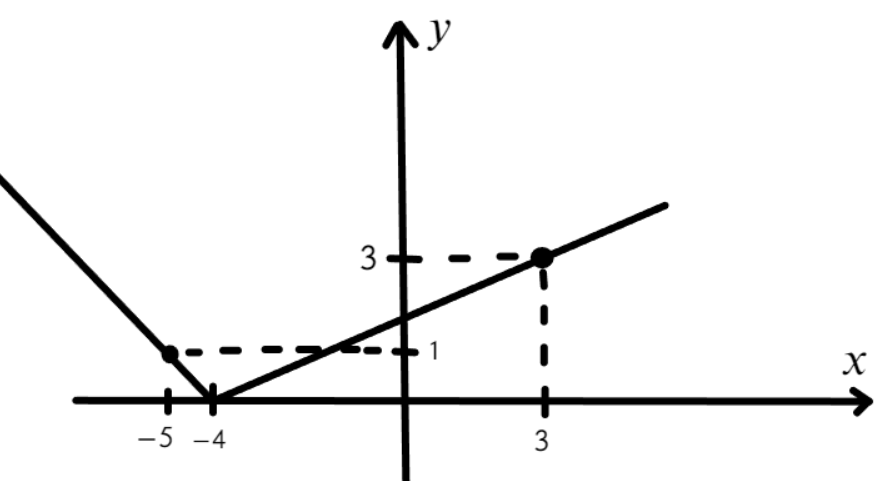
\includegraphics[scale=0.35]{gr8-101.png}}
\end{figure}\\
102. Построить множество точек, для которых выполнено условие:
$$\cfrac{(y+1)(2x^2-xy-y^2)}{x^2+xy-2y-4}=0.$$
103. а) Постройте график функции $g(x)=\cfrac{4\sqrt{x^2+4x+4}}{\sqrt{16+8x+x^2}+x}.$\\
б) С помощью построенного в предыдущем задании графика определите все значения $k,$ при каждом из которых прямая $y=k(x+2)$ имеет с данным графиком более одной общей точки.\\
104. а) Постройте график функции $g(x)=\cfrac{6\sqrt{x^2-2x+1}}{\sqrt{4-4x+x^2}-x}.$\\
б) С помощью построенного в предыдущем задании графика определите все значения $k,$ при каждом из которых прямая $y=k(x-1)$ имеет с данным графиком более одной общей точки.\\
105. Постройте график функции $y=\cfrac{2x(4x^2-1)}{2x^2-x}$ и определите, какие значения может принимать $y.$\\
106. Постройте график функции $y=\cfrac{2x(x^2-9)}{x^2-3x}$ и определите, какие значения может принимать $y.$\\
107. Изобразите множество точек, координаты которых удовлетворяют условию $(|x-2|-1)(y+x^2-2x-3)=0.$\\
108. а) Упростить выражение $\cfrac{(x^2+4x+3)(x-1)}{x+1}$ и построить график функции \\$f(x)=\cfrac{(x^2+4x+3)(x-1)}{x+1}.$\\
б) Найти все значения, которые принимает функция $f$ при $x\in[-2;1].$\\
109. Постройте график функции $\cfrac{x^2-10x+24}{|x-7|+|x-3|-2}.$\\
110. Постройте график функции $\cfrac{x^2-8x+15}{|x-6|+|x-2|-2}.$\\
111. Вершина параболы $y=f(x)$ расположена в точке $\left(\cfrac{7}{2};2\cfrac{3}{5}\right),$ а один из корней уравнения $f(x)=0$
равен $\sqrt{2}.$ Найдите второй корень.\\
112. Вершина параболы $y=f(x)$ расположена в точке $\left(\cfrac{5}{2};3\cfrac{2}{5}\right),$ а один из корней уравнения $f(x)=0$
равен $\sqrt{3}.$ Найдите второй корень.\\
113. На координатной плоскости проведены прямые $y=\cfrac{2}{3}x,\ y=4x,\ x+y=5.$ Найдите точки их пересечения и вычислите площадь треугольника
с вершинами в этих точках.\\
114. На координатной плоскости проведены прямые $y=\cfrac{4}{3}x,\ y=6x,\ x+y=7.$ Найдите точки их пересечения и вычислите площадь треугольника
с вершинами в этих точках.\\
115. Построить графики функций\\
а) $y=-x^2+4x-3;$\\
б) $y=-x^2+4|x|-3.$\\
116. Построить графики функций\\
а) $y=-x^2+2x-3;$\\
б) $y=-x^2+2|x|-3.$
\newpage
\section{Стандартные задачи}
1. При одновременной работе двух насосов пруд был очищен за 2 ч 55 мин. За сколько времени мог бы очистить пруд каждый насос, работая отдельно, если один из них может эту работу выполнить на 2 ч быстрее другого?\\
2. За 4 дня совместной работы двух тракторов различной мощности было вспахано $\cfrac{2}{3}$ поля. За сколько дней можно было бы вспахать всё поле каждым трактором в отдельности, если первым трактором это можно сделать на 5 дней быстрее, чем вторым?\\
3. Положительное число $a$ составляет $200\%$ от своего квадрата. Найдите число $a.$\\
4. Положительное число $a$ составляет $400\%$ от своего квадрата. Найдите число $a.$\\
5. Товар первоначально стоил $a$ рублей. Затем он подорожал на $10\%,$ а потом ещё на $15\%.$ На сколько процентов от первоначальной стоимости подорожал товар?\\
6. Товар первоначально стоил $a$ рублей. Затем он подорожал на $15\%,$ а потом ещё на $10\%.$ На сколько процентов от первоначальной стоимости подорожал товар?\\
7. Путь от города до посёлка автомобиль проезжает за 2,5 часа. Если он увеличит скорость на 20 км/ч, то за 2 часа он проедет путь на 15 км больше, чем расстояние от города до посёлка. Найти расстояние от города до посёлка.\\
8. Из Москвы в Санкт-Петербург выехал автобус. Спустя час вслед за ним вышла
легковая машина, скорость которой на 20 км/ч больше скорости автобуса. Машина обогнала автобус и через 5 часов после своего выхода находилась впереди него на 70 км. Найти скорость автобуса.\\
9. Саша и Стас вскапывают грядку за 10 минут, а один Стас за 15 минут. За сколько минут Саша один вскопает грядку?\\
10. Таня и Лена пропалывают грядку за 12 минут, а одна Лена за 20 минут. За сколько минут прополет грядку одна Таня?\\
11. На двух копировальных машинах, работающих одновременно, можно сделать копию пакета документов за 10 минут. За какое время можно выполнить эту работу на каждой машине в отдельности, если известно, что на первой машине её можно сделать на 15 минут быстрее, чем на второй?\\
12. На двух копировальных машинах, работающих одновременно, можно сделать копию пакета документов за 20 минут. За какое время можно выполнить эту работу на каждой машине в отдельности, если известно, что на первой машине её можно сделать на 30 минут быстрее, чем на второй?\\
13. Комната с размерами 4 метра и 6 метров составляет $75\%$ от всей квартиры. Найдите площадь квартиры.\\
14. Комната с размерами 3 метра и 4 метра составляет $60\%$ от всей квартиры. Найдите площадь квартиры.\\
15. Из А и В одновременно выехали 2 автомобиля. Первый проехал весь путь с постоянной скоростью. Второй проехал первую половину пути со скоростью 24 км/ч, а вторую половину пути --- со скоростью на 16 км/ч больше скорости первого, в результате чего прибыл в В одновременно с первым автомобилем. Найдите скорость первого автомобиля.\\
16. Из А и В одновременно выехали 2 автомобиля. Первый проехал весь путь с постоянной скоростью. Второй проехал первую половину пути со скоростью 33 км/ч, а вторую половину пути --- со скоростью на 22 км/ч больше скорости первого, в результате чего прибыл в В одновременно с первым автомобилем. Найдите скорость первого автомобиля.\\
17. Товар стоил $a$ рублей. Потом он подорожал на $10\%.$ После чего подешевел на $10\%$ от новой цены. Сколько стал стоить товар после удешевления?\\
18. Товар стоил $a$ рублей. Потом он подешевел на $10\%.$ После чего подорожал на $10\%$ от новой цены. Сколько стал стоить товар после подорожания?\\
19. Пароход прошёл 9 км по озеру и 20 км по течению реки за 1 час. Найти скорость парохода при движении по озеру, если скорость течения реки равна 3 км/ч.\\
20. Пароход прошёл 9 км по озеру и 16 км против течения реки за 1 час. Найти скорость парохода при движении по озеру, если скорость течения реки равна 3 км/ч.\\
21. Велосипедист проехал за 2,5 часа 58 км, а за следующий час ещё 19 км. Найдите среднюю скорость велосипедиста.\\
22. Велосипедист проехал за 1,5 часа 36 км, а за следующие 2 часа ещё 34 км. Найдите среднюю скорость велосипедиста.\\
23. Рубашка на $20\%$ дешевле пиджака. На сколько процентов пиджак дороже рубашки?\\
24. Из Санкт-Петербурга в Псков выехал автомобиль Москвич со скоростью 60 км/ч. В то же время навстречу ему из Пскова выехал автомобиль Жигули со скоростью 80 км/ч. Какое расстояние было между ними за час до встречи?\\
25. Сколько граммов воды надо добавить к 180 граммам сиропа, содержащего $25\%$ сахара, чтобы получить сироп, процентное содержание сахара в котором равно $20\%?$\\
26. Сколько граммов воды надо добавить к 220 граммам сиропа, содержащего $25\%$ сахара, чтобы получить сироп, процентное содержание сахара в котором равно $20\%?$\\
27. Цена билета на стадион была 150 рублей. После снижения цены билета количество посетителей увеличилось на $50\%,$ а сбор увеличился на $25\%.$ Найти новую цену билета.\\
28. Цена билета на стадион была 120 рублей. После снижения цены билета количество посетителей увеличилось на $50\%,$ а сбор увеличился на $25\%.$ Найти новую цену билета.\\
29. Одновременно из пункта А в одном направлении выехали два мотоциклиста: скорость одного из них 75 км/ч, а скорость второго 60 км/ч. Через 20 минут вслед за ними из пункта А выехал третий мотоциклист. Найдите скорость третьего мотоциклиста, если известно, что он догнал первого мотоциклиста на 1 час позже, чем второго. Ответ дайте в километрах в час.\\
30. Турист проплыл на байдарке 25 км по озеру и 9 км против течения реки за столько же времени, за сколько он проплыл бы по течению той же реки 56 км. Найдите скорость байдарки в стоячей воде, если скорость течения реки равна 2 км/ч. Ответ дайте в километрах в час.\\
31. Одновременно из пункта А в одном направлении выехали два велосипедиста: скорость одного из них 15 км/ч, а скорость второго 12 км/ч. Через 20 минут вслед за ними из пункта А выехал третий велосипедист. Найдите скорость третьего велосипедиста, если известно, что он догнал первого велосипедиста на 1 час позже, чем второго. Ответ дайте в километрах в час.\\
32. Турист проплыл на байдарке 15 км по озеру и 9 км против течения реки за столько же времени, за сколько он проплыл бы по течению той же реки 42 км. Найдите скорость байдарки в стоячей воде, если скорость течения реки равна 2 км/ч. Ответ дайте в километрах в час.\\
33. Торговая база закупила партию альбомов и поставила её магазину по оптовой цене на $130\%$ выше закупочной. Магазин установил розничную цену на альбом на $5\%$ выше оптовой. При распродаже в конце сезона магазин снизил розничную цену на альбом на $40\%.$ На сколько рублей больше заплатил покупатель по сравнению с закупочной ценой, если на распродаже он приобрёл альбом за 57,96 рубля?\\
34. Торговая база закупила партию альбомов и поставила её магазину по оптовой цене на $20\%$ выше закупочной. Магазин установил розничную цену на альбом на $110\%$ выше оптовой. При распродаже в конце сезона магазин снизил розничную цену на альбом на $30\%.$ На сколько рублей больше заплатил покупатель по сравнению с закупочной ценой, если на распродаже он приобрёл альбом за 123,48 рубля?\\
35. Торговая база закупила партию альбомов и поставила её магазину по оптовой цене на $5\%$ выше закупочной. Магазин установил розничную цену на альбом на $120\%$ выше оптовой. При распродаже в конце сезона магазин снизил розничную цену на альбом на $40\%.$ На сколько рублей больше заплатил покупатель по сравнению с закупочной ценой, если на распродаже он приобрёл альбом за 69,3 рубля?\\
36. Торговая база закупила партию альбомов и поставила её магазину по оптовой цене на $110\%$ выше закупочной. Магазин установил розничную цену на альбом на $5\%$ выше оптовой. При распродаже в конце сезона магазин снизил розничную цену на альбом на $30\%.$ На сколько рублей больше заплатил покупатель по сравнению с закупочной ценой, если на распродаже он приобрёл альбом за 92,61 рубля?\\
37. В банк 01.01.2014 г. положили 50000 р. 31 декабря каждого года банк увеличивает вклад на одно и то же число процентов. На какое число процентов ежегодно увеличивается вклад, если 01.01.2016 г. вклад составил 55125 р.?\\
38. В банк 01.01.2014 г. положили 2000 р. 31 декабря каждого года банк увеличивает вклад на одно и то же число процентов. На какое число процентов ежегодно увеличивается вклад, если 01.01.2016 г. вклад составил 2420 р.?\\
39. Один км от дома до остановки автобуса Петя проходит за 15 мин. Следующие 7 км на автобусе он проезжает за 12 мин. Затем 2 км от остановки до школы мальчик пробегает за 13 мин. Какова средняя скорость Пети в школу?\\
40. Спортсмен-триатлонист сначала проплыл 1 км за 15 мин, потом пробежал 10 км за 50 мин, затем проехал на велосипеде 29 км за 55 мин. Какова средняя скорость спортсмена?\\
41. На соревнованиях по кольцевой трассе один лыжник проходил круг на 3 минуты быстрее другого и через час обогнал его ровно на круг. За сколько минут каждый лыжник проходит круг?\\
42. На соревнованиях по кольцевой трассе один лыжник проходил круг на 5 минут быстрее другого и через час обогнал его ровно на круг. За сколько минут каждый лыжник проходит круг?\\
43. Свежий виноград содержит $80\%$ влаги, а сушёный виноград (изюм) --- $5\%.$ Сколько требуется свежего винограда для приготовления 1 кг изюма?\\
44. Винни Пух и Пятачок могут изготовить подарок ослику Иа-Иа за 8 дней. Определите, за сколько дней Пятачок изготовит этот подарок, работая отдельно, если известно, что он сделает это на 12 дней быстрее, чем Винни.\\
45. Малыш и Карлсон вместе съедают банку варенья за 12 минут. Определите, за сколько минут справится с банкой варенья Карлсон, если известно, что он сделает это на 10 минут быстрее, чем Малыш.\\
46. Из Петербурга в Москву одновременно отправились курьер и гонец. Курьер проехал с постоянной скоростью весь путь. Гонец проехал первую половину пути со скоростью 102 км/ч, а вторую половину пути --- со скоростью, на 17 км/ч меньшей скорости курьера, в результате чего прибыл в Москву одновременно с курьером. Известно, что скорость курьера меньше 60 км/ч. Найдите скорость курьера.\\
47. Из Москвы в Петербург одновременно выехали генерал и чиновник. Генерал проехал с постоянной скоростью весь путь. Чиновник проехал первую половину пути со скоростью, меньшей скорости генерала на 13 км/ч, а вторую половину пути --- со скоростью 78 км/ч, в результате чего прибыл в Петербург одновременно с генералом. Найдите скорость генерала, если известно, что она больше 48 км/ч.\\
48. После того, как рабочий увеличил производительность своего труда на $16\%,$ он сократил на 1 час время выполнения задания. Сколько времени теперь он стал тратить на выполнение этого задания?\\
49. Смешали 30 г $20\%$-го раствора соли с 10 г другого раствора и получили раствор с концентрацией соли $25\%.$ Определить концентрацию соли во втором растворе.\\
50. Если велосипедист увеличит скорость на 5 км/ч, то получит выигрыш во времени 12 минут при прохождении некоторого пути. Если же он уменьшит скорость на 8 км/ч, то потеряет 40 минут на том же пути. Найдите скорость велосипедиста и длину пути.\\
51. Численность волков в двух заповедниках составляла 210 особей. Через год обнаружили, что в первом заповеднике численность волков выросла на $10\%,$ а во втором --- на $30\%.$ В результате общая численность волков в этих двух заповедниках составила 251 особь. Сколько волков было в каждом из двух заповедников первоначально?\\
52. Сколько граммов четырёхпроцентного и сколько граммов девятипроцентного растворов соли необходимо взять, чтобы получить 250 граммов её шестипроцентного раствора?\\
53. Некоторый товар стоил 1000 рублей, но не пользовался спросом. Поэтому его цена дважды снижалась на $40\%$ и один раз на $20\%.$ Сколько стал стоить этот товар после последнего снижения цены?\\
54. Некоторый товар стоил 1000 рублей, но не пользовался спросом. Поэтому его цена дважды снижалась на $20\%$ и один раз на $60\%.$ Сколько стал стоить этот товар после последнего снижения цены?\\
55. Мотоциклист задержался с выездом на 9 минут. Чтобы наверстать потерянное время, он увеличил намеченную скорость на 10 км/ч. С какой скоростью ехал мотоциклист, если весь путь равен 30 км?\\
56. Петя вышел из школы и пошёл домой со скоростью 4,5 км/ч. Через 20 минут по той же дороге из школы выехал Вася на велосипеде со скоростью 12 км/ч. На каком расстоянии от школы Вася догонит Петю?\\
57. Нина поехала на велосипеде на рынок со скоростью 15 км/ч. Через 6 минут по той же дороге поехал на мопеде её брат со скоростью 40 км/ч. На каком расстоянии от дома брат догонит Нину?\\
58. Сколько граммов $15\%$-ного раствора соли надо добавить к 50 г $60\%$-ного раствора соли, чтобы получить $40\%$-ный раствор соли?\\
59. Сколько граммов $75\%$-ного раствора кислоты надо добавить к 30 г $15\%$-ного раствора кислоты, чтобы получить $50\%$-ный раствор кислоты?\\
60. По двум параллельным железнодорожным путям в одном направлении следуют пассажирский и товарный поезда, скорости которых равны 70 км/ч и 30 км/ч. Длина товарного поезда равна 1400 метрам. Найдите длину пассажирского поезда, если время, за которое он прошел мимо товарного поезда, равно 3 минутам.\\
61. По двум параллельным железнодорожным путям в одном направлении следуют пассажирский и товарный поезда, скорости которых равны 75 км/ч и 45 км/ч. Длина товарного поезда равна 800 метрам. Найдите длину пассажирского поезда, если время, за которое он прошел мимо товарного поезда, равно 2 минутам.\\
62. В сосуд, содержащий 7 литров 14-процентного раствора некоторого вещества, добавили 21 литр воды. Сколько процентов составляет концентрация полученного раствора?\\
63. В сосуд, содержащий 5 литров 12-процентного раствора некоторого вещества, добавили 7 литров воды. Сколько процентов составляет концентрация полученного раствора?\\
64. Повысив скорость на 10 км/ч, поезду удалось сократить на 1 час время, затрачиваемое на прохождение 720 км. Найти первоначальную скорость поезда.\\
65. Повысив скорость на 10 км/ч, поезду удалось сократить на 1 час время, затрачиваемое на прохождение 560 км. Найти первоначальную скорость поезда.\\
66. Смешали 8 литров $25\%$ водного раствора некоторого вещества с 12 литрами $20\%$ водного раствора этого же вещества. Сколько процентов составляет концентрация получившегося раствора?\\
67. Смешали 4 литра $15\%$ водного раствора некоторого вещества с 6 литрами $25\%$ водного раствора этого же вещества. Сколько процентов составляет концентрация получившегося раствора?\\
68. Два велосипедиста одновременно отправились в 88-километровый пробег. Первый ехал со скоростью на 3 км/ч большей, чем скорость второго, и прибыл к финишу на 3 часа раньше второго. Найти скорость велосипедиста, пришедшего к финишу вторым. Ответ дайте в км/ч.\\
69. Два велосипедиста одновременно отправились в 96-километровый пробег. Первый ехал со скоростью на 4 км/ч большей, чем скорость второго, и прибыл к финишу на 4 часа раньше второго. Найти скорость велосипедиста, пришедшего к финишу вторым. Ответ дайте в км/ч.\\
70. При температуре $0^\circ C$ рельс имеет длину $l_0=10$м. При возрастании температуры происходит тепловое расширение рельса, и его длина, выраженная в метрах, меняется по закону:
$$l(t^\circ)=l_0(1+\alpha\cdot t^\circ),$$
где $\alpha=1,2\cdot10^{-5}(^\circ C)^{-1}$ --- коэффициент теплового расширения, $t^\circ$ --- температура (в градусах Цельсия). При какой температуре рельс удлинится на 3 мм? Ответ выразите в градусах Цельсия.\\
71. Морская вода содержит $5\%$ соли (по весу). Сколько кг пресной воды нужно прибавить к 40 кг морской воды, чтобы содержание соли составило $2\%?$\\
72. Смешали какое-то количество 40-процентного и 75-процентного раствора кислоты, в результате чего получился 61-процентный раствор кислоты. Если бы каждого раствора взяли на 40 литров меньше, то получился бы 65-процентный раствор. Сколько литров каждого раствора было взято первоначально?\\
73. Смешали какое-то количество 30-процентного и 65-процентного раствора кислоты, в результате чего получился 55-процентный раствор кислоты. Если бы каждого раствора взяли на 20 литров больше, то получился бы 51-процентный раствор. Сколько литров каждого раствора было взято первоначально?\\
74. Двое бегают вокруг озера. Скорость каждого постоянна и на один круг один из них тратит на 7 минут меньше другого. Если они начинают бежать с общего старта одновременно и в одном направлении, то впервые встретятся через 1 ч 24 мин. Через какое время они впервые встретятся, если побегут одновременно с общего старта в противоположных направлениях?\\
75. Двое бегают вокруг озера. Скорость каждого постоянна и на один круг один из них тратит на 9 минут меньше другого. Если они начинают бежать с общего старта одновременно в противоположных направлениях, то впервые встретятся через 20 мин. Через какое время они впервые встретятся, если побегут одновременно с общего старта в одном направлении?\\
76. Первые два часа автомобиль ехал со скоростью 50 км/ч, следующий час --- со скоростью 100 км/ч, а затем два часа --- со скоростью 75 км/ч. Найдите среднюю скорость автомобиля на протяжении всего пути. Ответ дайте в км/ч.\\
77. Первые 190 км автомобиль ехал со скоростью 50 км/ч, следующие 180 км --- со скоростью 90 км/ч, а затем 170 км --- со скоростью 100 км/ч. Найдите среднюю скорость автомобиля на протяжении всего пути. Ответ дайте в км/ч.\\
78. Имеются два раствора серной кислоты в воде: первый --- $40\%,$ а второй --- $60\%.$ Эти растворы смешали, после чего добавили 5 кг чистой воды и получили $20\%$-й раствор. Если бы вместо 5 кг чистой воды добавили 5 кг $80\%$-го раствора, то получился бы $70\%$-й раствор. Сколько было $40\%$-го и $60\%$-го растворов?\\
79. Смешав $30\%$ и $60\%$ растворы кислоты и добавив 10 кг чистой воды, получили $36\%$ раствор кислоты. Если бы вместо 10 кг воды добавили 10 кг $50\%$ раствора той же кислоты, то получили бы $41\%$ раствор кислоты. Сколько килограммов $30\%$ и $60\%$ растворов использовали для получения смеси?\\
80. Водный раствор соли содержал 60 г чистой воды и $x\%$ соли. После того как в раствор добавили 20 г чистой воды, масса соли стала составлять $(x-5)\%$ массы раствора. Сколько граммов соли содержит раствор?\\
81. Из города $A$ в город $B,$ находящийся на расстоянии 20 километров от него, выехал трактор,
а через 5 минут ему навстречу выехал второй трактор, скорость которого была на 5 км/ч больше. Второй трактор приехал в $A$
на 3 минуты раньше, чем первый в $B.$ Найдите скорость второго трактора.\\
82. Из города $A$ в город $B,$ находящийся на расстоянии 15 километров от него, выехал трактор,
а через 5 минут ему навстречу выехал второй трактор, скорость которого была на 5 км/ч больше. Второй трактор приехал в $A$
на 4 минуты раньше, чем первый в $B.$ Найдите скорость второго трактора.\\
83. Цену на товар подняли на $30\%,$ а зарплату на $4\%.$ На сколько процентов меньше товара теперь удастся купить на зарплату?\\
84. Цену на товар подняли на $70\%,$ а зарплату на $2\%.$ На сколько процентов меньше товара теперь удастся купить на зарплату?\\
85. Бак наполнен спиртом. Из бака вылили часть спирта и
дополнили его водой. Потом из бака вылили столько же
литров смеси. В баке осталось 49 литров спирта. Сколько
литров спирта вылили в первый раз и сколько во второй
раз, если вместимоcть бака 64 литра?\\
86. Имеется два тридцатилитровых сосуда, в которых
содержится всего 30 л спирта. Первый сосуд доливают
доверху водой и полученной смесью дополняют второй
сосуд, из которого затем переливают 12 л новой смеси в
первый. Сколько литров спирта было сначала в каждом
сосуде, если во втором оказалось на 2 литра спирта
меньше, чем в первом.\\
87. Из пунктов $A$ и $B,$ расстояние между которыми равно 19
км, вышли одновременно навстречу друг другу два
пешехода и встретились в 9 км от $A.$ Найдите скорость
пешехода, шедшего из $A,$ если он шёл со скоростью на
1 км/ч большей, чем пешеход, шедший из $B,$ и сделал в
пути получасовую остановку.\\
88. Из пунктов $A$ и $B,$ расстояние между которыми равно 27
км, вышли одновременно навстречу друг другу два
пешехода и встретились в 15 км от $A.$ Найдите скорость
пешехода, шедшего из $A,$ если он шел со скоростью на
2 км/ч большей, чем пешеход, шедший из $B,$ и сделал в
пути получасовую остановку.
\newpage
\section{Нестандартные задачи}
1. Наибольший общий делитель целых чисел a и b равен 1. Доказать, что
НОД$(a, a+b)=1.$\\
2. Наибольший общий делитель целых чисел a и b равен 1. Доказать, что
НОД$(a, a-b)=1.$\\
3. Найдите все натуральные $n,$ при которых число $\cfrac{3n-1}{n+1}$ является целым.\\
4. Найдите все натуральные $n,$ при которых число $\cfrac{3n+1}{n-1}$ является целым.\\
5. В магазине продаются раки: маленькие --- по 5 рублей, большие --- по 7 рублей. Сколько маленьких и больших раков можно купить на 101 рубль ровно?\\
6. В магазине продаются раки: маленькие --- по 5 рублей, большие --- по 8 рублей. Сколько маленьких и больших раков можно купить на 116 рублей ровно?\\
7. При каких целых $n$ число $\cfrac{4n-5}{2n-1}$ будет целым?\\
8. При каких целых $n$ число $\cfrac{4n+5}{2n+1}$ будет целым?\\
9. Сколько различных диагоналей можно провести в выпуклом семиугольнике?\\
10. Сколько различных диагоналей можно провести в выпуклом восьмиугольнике?\\
11. Найти наибольшее двузначное натуральное число $n$ такое, что $\cfrac{3n+17}{n+4}$ --- сократимая дробь.\\
12. Найти наибольшее двузначное натуральное число $n$ такое, что $\cfrac{3n+16}{n+4}$ --- сократимая дробь.\\
13. На столе лежат книги, число которых меньше 100. Сколько лежит книг, если их можно без остатка связать в пачки как по 3, так и по 4 и по 5 книг?\\
14. На столе лежат книги, число которых меньше 100. Сколько лежит книг, если их можно без остатка связать в пачки как по 3, так и по 4 и по 7 книг?\\
15. Решить уравнение в целых числах: $2x^2+xy=x+7.$\\
16. Решить уравнение в целых числах: $x^2-3xy=x-3y+2.$\\
17. Найдите наименьшее трёхзначное число, сумма цифр которого равна 22.\\
18. Найдите наименьшее трёхзначное число, сумма цифр которого равна 23.\\
19. <<Зенит>>, <<Спартак>> и ЦСКА стали призёрами первенства России по футболу. Сколькими способами они могут расположиться на первых трёх местах?\\
20. Сколькими способами можно раздать яблоко, мандарин и грушу Пете, Саше и Гале так, чтобы каждому досталось по одному фрукту?\\
21. Пусть $a$ --- чётное число, не кратное 6. Найти остаток от деления числа $a^2$ на 12.\\
22. Пусть $a$ --- целое число, не кратное 3. Найти остаток от деления числа $a^2$ на 3.\\
23. Число $n$ при делении на 5 даёт в остатке 4. Найти остаток от деления числа $(4n+3)$ на 5.\\
24. Число $n$ при делении на 4 даёт в остатке 3. Найти остаток от деления числа $(3n+2)$ на 4.\\
25. Сколько двузначных чисел делятся без остатка на 4 и на 6?\\
26. Сколько двузначных чисел делятся без остатка на 6 и на 9?\\
27. Решить уравнение $x^{1024}+1=\cfrac{1}{2+x^{318}}.$\\
28. Решить уравнение $x^{1024}+2=\cfrac{1}{1+x^{318}}.$\\
29. Решить в целых числах $x\cdot (y-2)=3,$ если известно, что $x<0.$\\
30. Решить в целых числах $x\cdot (y-4)=3,$ если известно, что $x<0.$\\
31. Из Петербурга в Москву можно проехать двумя способами, а из Москвы в Братск четырьмя способами. Сколькими способами можно проехать из Петербурга в Братск?\\
32. Из Петербурга в Москву можно проехать двумя способами, а из Москвы в Хабаровск пятью способами. Сколькими способами можно проехать из Петербурга в Хабаровск?\\
33. В шахматном турнире принимают участие 7 игроков. Сколько нужно сыграть игр, чтобы каждый шахматист сыграл с каждым?\\
34. В январе было 5 понедельников. Какое наибольшее число четвергов могло быть в этом январе?\\
35. В марте было 5 вторников. Какое наибольшее число пятниц могло быть в этом марте?\\
36. В кубе с ребром 10 см все грани покрасили в разные цвета. Затем куб разрезали на 1000 кубиков со стороной в 1 см. Сколько получилось кубиков, у которых ровно две грани окрашены в разные цвета?\\
37. В кубе с ребром 1 м все грани покрасили в разные цвета. Затем куб разрезали на 1000 кубиков со стороной в 10 см. Сколько получилось кубиков, у которых ровно две грани окрашены в разные цвета?\\
38. В карточной колоде 36 карт, по девять каждой масти. Мы берём двух королей. Сколько различных пар мы можем получить?\\
39. В карточной колоде 36 карт, по девять каждой масти. Мы берём двух валетов. Сколько различных пар мы можем получить?\\
40. Наименьшее общее кратное чисел $a$ и $b$ равно $\cfrac{ab}{3}.$ Найдите их наибольший общий делитель.\\
41. Наименьшее общее кратное чисел $a$ и $b$ равно $\cfrac{ab}{5}.$ Найдите их наибольший общий делитель.\\
42. На окружности взяли 7 точек и провели через них всевозможные хорды. Сколько всего хорд провели?\\
43. На окружности взяли 6 точек и провели через них всевозможные хорды. Сколько всего хорд провели?\\
44. Произвольному многочлену $P(x)$ ставится в соответствие многочлен $P'(x)$ так, что выполнялись следующие правила:\\
1. Для любых двух многочленов $P_1(x)$ и $P_2(x): \left(P_1(x)+P_2(x)\right)'=P_1'(x)+P_2'(x);$\\
2. Для любого числа $a$ и многочлена $P(x): (a\cdot P(x))'=a\cdot P'(x);$\\
3. Если $P(x)=x^n,$ то $P'(x)=n\cdot x^{n-1}.$\\
Найдите $P'(x),$ если:\\
а) $P(x)=3x^5+4x^3;$\\
б) $P(x)=1$ для любого $x,$ т.е. $P(x)\equiv 1;$\\
в) $P(x)=(T'(x)+3xT(x))'-18x^2-45x^4,$ где $T(x)=3x^4-2x^2.$\\
45. Произвольному многочлену $P(x)$ ставится в соответствие многочлен $P'(x)$ так, что выполнялись следующие правила:\\
1. Для любых двух многочленов $P_1(x)$ и $P_2(x): \left(P_1(x)+P_2(x)\right)'=P_1'(x)+P_2'(x);$\\
2. Для любых двух многочленов $P_1(x)$ и $P_2(x): (P_1(x)\cdot P_2(x))'=P_1'(x)\cdot P_2(x)+P_1(x)\cdot P_2'(x);$\\
3. Для любого числа $a$ и многочлена $P(x): (a\cdot P(x))'=a\cdot P'(x);$\\
4. Если $P(x)=x,$ то $P'(x)=1.$\\
5. Если $P(x)=x^3,$ то $P'(x)=3\cdot x^2.$\\
а) Найдите $P'(x),$ если $P(x)=3x^3+4x;$\\
б) Найдите $P'(x),$ если $P(x)=x^6-2x^4;$\\
в) Найдите $P(x),$ если $P(x)=(T(x)+3xT(x))'-9x^2-36x^3,$ где $T(x)=3x^3-2x.$\\
46. Сколько трёхзначных нечётных чисел можно составить из цифр 0, 1, 4, 5, если цифры числа могут повторяться?\\
47. Сколько трёхзначных чётных чисел можно составить из цифр 0, 1, 4, 5, если цифры числа могут повторяться?\\
48. Бросаются 2 игральные кости. Найдите вероятность того, что сумма выпавших очков равна 10.\\
49. Бросаются 2 игральные кости. Найдите вероятность того, что сумма выпавших очков равна 4.\\
50. В шахматном турнире принимали участие 15 шахматистов, причём каждый из них сыграл только одну партию с каждым из остальных. Сколько всего партий было сыграно в этом турнире?\\
51. В шахматном турнире принимали участие 14 шахматистов, причём каждый из них сыграл только одну партию с каждым из остальных. Сколько всего партий было сыграно в этом турнире?\\
52. Конференция длится три дня. В первый и второй день выступают по 15 докладчиков, в третий день --- 20. Какова вероятность того, что доклад профессора М. выпадет на третий день, если порядок докладов определяется жеребьёвкой?\\
53. Конференция длится три дня. В первый и второй день выступают по 20 докладчиков, в третий день --- 10. Какова вероятность того, что доклад профессора М. выпадет на третий день, если порядок докладов определяется жеребьёвкой?\\
54. Остаток от деления числа $a$ на 3 равен 1. Найти остаток от деления числа $a^2$ на 3.\\
55. Остаток от деления числа $a$ на 5 равен 1. Найти остаток от деления числа $a^2$ на 5.\\
56. Введём новое число $\Game,$ такое, что $\Game^2=-1,$ а все остальные арифметические операции с ним и другими числами происходят как обычно. Говорят, что выражение имеет {\it не раздражающий} вид, если оно имеет вид $a+b\cdot\Game,$ где $a$ и $b$ вещественные числа.

Запишите в {\it не раздражающем} виде следующее выражение:
$$(4\cdot\Game-1)\cdot(4\cdot\Game+1)-17\cdot\Game\cdot(\Game-2).$$
57. Введём новое число $\Game,$ такое, что $\Game^2=-1,$ а все остальные арифметические операции с ним и другими числами происходят как обычно. Говорят, что выражение имеет {\it не раздражающий} вид, если оно имеет вид $a+b\cdot\Game,$ где $a$ и $b$ вещественные числа.

Запишите в {\it не раздражающем} виде следующее выражение:
$$(3\cdot\Game-1)\cdot(3\cdot\Game+1)-10\cdot\Game\cdot(\Game-2).$$
58. Числитель дроби $\cfrac{k}{n}$ (здесь $k$ и $n$ --- натуральные числа) увеличили на 1, а её знаменатель --- на 2. Выясните, будет ли полученная дробь меньше или же больше исходной.\\
59. Найдите наименьшее значение выражения $\cfrac{5x^2+10x+14}{x^2+2x+3}.$\\
60. Найдите наибольшее значение выражения $\cfrac{x^2+2x+5}{x^2+2x+3}.$\\
61. Красные карандаши стоят 17 руб за штуку, синие --- 13 руб. Нужно купить карандаши на сумму 495 рублей, причём число красных не должно отличаться от числа синих более чем на 5 штук.\\
а) Можно ли купить 32 карандаша? (ответ обосновать)\\
б) Можно ли купить 35 карандашей? (ответ обосновать)\\
в) Какое наибольшее количество карандашей можно купить при таких условиях? (ответ обосновать)\\
62. Найти наибольшее значение выражения $\cfrac{x^2-4x+7}{x^2-4x+5}.$\\
63. Натуральные числа $a$ и $b$ таковы, что $19a=97b.$ Докажите, что их сумма $(a+b)$ делится на 116.\\
64. Найдите $\cfrac{a}{b+c}+\cfrac{b}{a+c}+\cfrac{c}{a+b},$ если $a+b+c=7$ и $\cfrac{1}{b+c}+\cfrac{1}{a+c}+\cfrac{1}{a+b}=\cfrac{7}{10}.$\\
65. Найдите все целые значения $n$ таких, что $\sqrt{n^2-17}$ --- целое число.\\
66. Найдите количество различных делителей числа $6^{15}\cdot21^{7}.$\\
67. Если между цифрами двузначного числа $a$ вписать это же число, то полученное четырёхзначное число будет в 99 раз больше этого двузначного числа. Найдите двузначное число $a.$\\
68. На странице во всех строках одно и то же число букв. Если увеличить число строк и число букв в строке на 7, то число букв на странице увеличится на 476. На сколько уменьшится число букв на странице, если уменьшить число строк и число букв в строке на 4?\\
69. Найдите наибольшее двузначное число $n$ при котором остаток от деления числа $3^n$ на 7 равен 5, если такое число $n$ существует.\\
70. При каких натуральных $m$ и $n$ выполнено равенство $\cfrac{2}{m}+\cfrac{1}{n-1}=3?$\\
71. При каких натуральных $m$ и $n$ выполнено равенство $\cfrac{2}{m-1}+\cfrac{1}{n}=3?$\\
72. Найдите все целые значения $n,$ при каждом из которых значение выражения $\cfrac{12n+70}{4n+11}$ является целым числом.\\
73. Найдите все целые значения $n,$ при каждом из которых значение выражения $\cfrac{15n+58}{5n+9}$ является целым числом.\\
74. Значение выражения $ax^2+by^2+cz^2$ при $x=5,\ y=-3,\ z=-2$ равно 16. Найдите значение данного выражения при $x=\cfrac{25}{4},\ y=-\cfrac{15}{4},\ z=-\cfrac{5}{2}.$\\
75. Значение выражения $ax^2+by^2+cz^2$ при $x=4,\ y=-3,\ z=2$ равно 4. Найдите значение данного выражения при $x=10,\ y=-\cfrac{15}{2},\ z=5.$\\
76. Решите уравнение в целых числах: $(x-2)(y+3)=2.$\\
77. Решите уравнение в целых числах: $(x+2)(y-3)=2.$\\
78. Найдите такие натуральные $a,\ b$ и $c,$ что $a\cdot29+b\cdot30+c\cdot31=366.$\\
79. Найти наибольший общий делитель чисел 1394 и 1581.\\
80. Найти наибольший общий делитель чисел 1378 и 1599.\\
81. Сколькими способами можно выбрать двух дежурных из 30 человек в классе?\\
82. Сколькими способами можно выбрать двух дежурных из 20 человек в классе?\\
83. Звёздочкой обозначают знаки <<$+$>> или <<$-$>> совершенно произвольно. Может ли выполняться равенство $1*2*3*4*5*6*7*8*9=20?$\\
84. Звёздочкой обозначают знаки <<$+$>> или <<$-$>> совершенно произвольно. Может ли выполняться равенство $1*2*3*4*5*6*7*8*9=30?$\\
85. Из трёхзначного числа вычли сумму его цифр. Может ли разность оказаться равной 186?\\
86. Найдите все тройки натуральных чисел $(x;y;z),$ для которых $x^2+2xy+y^2-z^2=5.$\\
87. Найдите все тройки натуральных чисел $(x;y;z),$ для которых $x^2+2xy+y^2-z^2=7.$\\
88. а) Покажите, что данные числа являются квадратами натуральных чисел:\\
$a=2\cdot3\cdot4\cdot5+1;\qquad b=3\cdot4\cdot5\cdot6+1;\qquad c=7\cdot8\cdot9\cdot10+1.$\\
б) Обобщите имеющуюся закономерность и докажите её.\\
89. а) Покажите, что данные числа являются квадратами натуральных чисел:\\
$a=1+5\cdot4\cdot3\cdot2;\qquad b=1+6\cdot5\cdot4\cdot3;\qquad c=1+10\cdot9\cdot8\cdot7.$\\
б) Обобщите имеющуюся закономерность и докажите её.\\
90. На полке в шкафу стоят 5 колб. Известно, что только в одной из них противоядие, в остальных же --- яд. Но только на одной из колб надпись правдива. В какой колбе находится противоядие? Надписи на колбах по порядку: <<В №2 --- противоядие>>, <<Тут и в №1 --- яд>>, <<Тут и в №4 --- яд>>, <<Противоядие в №3 или в №5>>,
<<Тут и в №4 --- яд>>.\\
91. Найдите количество трёхзначных чисел, делящихся на 6, в записи которых встречается цифра 7.\\
92. Найдите количество трёхзначных чисел, делящихся на 6, в записи которых встречается цифра 5.\\
93. Решите уравнение в целых числах $x(x+2)=y^2+30.$\\
94. Решите уравнение в целых числах $y(y-2)=x^2+28.$\\
95. а) Можно ли число 2023 представить в виде суммы двух натуральных чисел, суммы цифр которых равны?\\
б) Можно ли число 799 представить в виде суммы двух натуральных чисел, суммы цифр которых равны?\\
в) Найдите наименьшее натуральное число, которое можно представить в виде суммы пяти различных натуральных чисел, суммы цифр которых равны.\\
96. а) Можно ли число 2021 представить в виде суммы двух натуральных чисел, суммы цифр которых равны?\\
б) Можно ли число 599 представить в виде суммы двух натуральных чисел, суммы цифр которых равны?\\
в) Найдите наименьшее натуральное число, которое можно представить в виде суммы шести различных натуральных чисел, суммы цифр которых равны.\\
97. По кругу в некотором порядке по одному разу написаны натуральные числа от 9 до 18. Для каждой из десяти пар соседних чисел нашли их наибольший общий делитель. а) Могло ли получиться так, что все наибольшие общие делители равны 1? б) Могло ли получиться так, что все наибольшие общие делители попарно различны?\\
98. Найти все двузначные числа, которые в четыре раза больше суммы своих цифр.\\
99. При каких натуральных $n$ число $\cfrac{7n-11}{8-n}$ будет натуральным?\\
100. При каких натуральных $n$ число $\cfrac{8n-13}{11-n}$ будет натуральным?\\
101. Сколько существует трёхзначных чисел, из которых перестановками цифр можно получить число большее 879?\\
102. Сколько существует трёхзначных чисел, из которых перестановками цифр можно получить число большее 769?
\newpage
\section{Геометрия задачи}
1. В трапеции $ABCD$ ($AD$ и $BC$ --- основания) диагонали пересекаются в точке $O.$ Доказать, что $S_{\Delta AOB}=S_{\Delta COD}.$\\
2. На стороне $BC$ параллелограмма $ABCD$ взяты произвольные точки $M$ и $K$ так, что отрезки $DM$ и $AK$ пересекаются в точке $O.$ Доказать, что $S_{\Delta AOM}=S_{\Delta KOD}.$\\
3. На каждой медиане равностороннего треугольника $ABC$ взята точка, делящая её в отношении $1:3,$ считая от вершины. Указанные точки обозначим $A_1,\ B_1,\ C_1.$ Найти отношение площадей треугольников $A_1B_1C_1$ и $ABC.$\\
4. На каждой медиане равностороннего треугольника $ABC$ взята точка, делящая её в отношении $1:4,$ считая от вершины. Указанные точки обозначим $A_1,\ B_1,\ C_1.$ Найти отношение площадей треугольников $A_1B_1C_1$ и $ABC.$\\
5. В прямоугольном треугольнике $ABC$ медиана $CM=12$см, а расстояние от середины катета $AC$ до гипотенузы $AB$ равно 3 см. Найдите площадь треугольника $ABC.$\\
6. В прямоугольном треугольнике $ABC$ медиана $CM=8$см, а расстояние от середины катета $AC$ до гипотенузы $AB$ равно 2 см. Найдите площадь треугольника $ABC.$\\
7. Средняя линия трапеции делится двумя диагоналями на три равные части. Найти отношение между основаниями трапеции.\\
8. Средняя линия трапеции равна 8 см и делится диагональю на два отрезка, разность между которыми равна 2 см. Найти основания трапеции.\\
9. Угол, противолежащий основанию равнобедренного треугольника, равен $120^\circ.$ Высота, проведённая к боковой стороне, равна 9 см. Найти основание треугольника.\\
10. Угол, противолежащий основанию равнобедренного треугольника, равен $120^\circ.$ Основание равно 8 см. Найти длину высоты, проведённой к боковой стороне.\\
11. Найти площадь прямоугольной трапеции, у которой две меньшие стороны равны 6 см, а больший угол $135^\circ.$\\
12. Найти площадь прямоугольной трапеции, у которой две меньшие стороны равны 4 см, а меньший угол $45^\circ.$\\
13. Найти углы ромба, если его диагонали равны $2\sqrt{3}$ и $2.$\\
14. Найти углы ромба, если его диагонали равны $4\sqrt{3}$ и $4.$\\
15. К окружности проведены касательная и секущая, проходящая через центр окружности. Длина касательной в два раза меньше длины секущей. Найти отношение длины касательной к длине радиуса.\\
16. К окружности проведены касательная и секущая, проходящая через центр окружности. Длина касательной в три раза меньше длины секущей. Найти отношение длины радиуса окружности к длине касательной.\\
17. Точка $M$ лежит на стороне $BC$ параллелограмма $ABCD,$ причём $BM:MC=3:1.$ Выразите вектор $\overrightarrow{AM}$ через векторы $\overrightarrow{AD}$ и $\overrightarrow{AB}.$\\
18. Точка $M$ лежит на стороне $BC$ параллелограмма $ABCD,$ причём $BM:MC=3:1.$ Выразите вектор $\overrightarrow{MD}$ через векторы $\overrightarrow{AD}$ и $\overrightarrow{AB}.$\\
19. На прямой $l$ найдите точку $C$ такую, чтобы сумма расстояний $AC+BC$ была наименьшей.
$$\begin{tikzpicture}[scale=1]
\tikzset {line01/.style={line width =0.5pt}}
\tikzset{line02/.style={line width =1pt}}
\tikzset{line03/.style={dashed,line width =0.9pt}}
\filldraw [black] (-2.5,1) circle (2pt);
\filldraw [black] (2.8,0.3) circle (2pt);
\draw[line01] (-3,0) -- (3,0);
\draw (2.9,0.6) node {\scriptsize $B$};
\draw (-2.5,0.6) node {\scriptsize $A$};
\draw (3.2,0) node {\scriptsize $l$};
\end{tikzpicture}$$
20. На прямой $l$ найдите точку $C$ такую, чтобы сумма расстояний $AC+BC$ была наименьшей.
$$\begin{tikzpicture}[scale=1]
\tikzset {line01/.style={line width =0.5pt}}
\tikzset{line02/.style={line width =1pt}}
\tikzset{line03/.style={dashed,line width =0.9pt}}
\filldraw [black] (-2.5,-1) circle (2pt);
\filldraw [black] (2.8,-0.3) circle (2pt);
\draw[line01] (-3,0) -- (3,0);
\draw (2.9,-0.6) node {\scriptsize $B$};
\draw (-2.5,-0.6) node {\scriptsize $A$};
\draw (3.2,0) node {\scriptsize $l$};
\end{tikzpicture}$$
21. Дан $ABCD$ --- прямоугольник. $AB=8,\ BC=4.$ На сторонах $AB$ и $CD$ отмечены точки $K$ и $P$ соответственно так, что $AK:AB=CP:CD=3:8.$\\
а) Докажите, что $KBPD$ --- ромб.\\
б) Найдите его периметр и площадь.\\
22. Две окружности, радиусы которых равны 8 и 2, касаются внешним образом. $AB$ --- их общая внешняя касательная ($A$ и $B$ --- точки касания). Найдите длину отрезка $AB.$\\
23. В треугольнике $ABC$ угол $B$ равен $80^\circ.\ M$ --- точка пересечения биссектрис углов $A$ и $C.$ Найти угол $AMC.$\\
24. В треугольнике $ABC$ угол $B$ равен $100^\circ.\ M$ --- точка пересечения биссектрис углов $A$ и $C.$ Найти угол $AMC.$\\
25. Найти диагонали ромба, если одна из них в 1,5 раза больше другой, а площадь ромба равна $27\text{см}^2.$\\
26. Найти диагонали ромба, если одна из них в 2,5 раза больше другой, а площадь ромба равна $20\text{см}^2.$\\
27. Найти площадь четырёхугольника $ABCD,$ если $AB=5,\ BC=13,\ CD=9,\ DA=15$ и $AC=12.$\\
28. Найти площадь четырёхугольника $ABCD,$ если $AB=12,\ BC=8,\ CD=17,\ DA=9$ и $BD=15.$\\
29. В равнобедренной трапеции, описанной  около круга, основания равны 36см и 100см. Найти радиус круга.\\
30. В равнобедренной трапеции, описанной  около круга, основания равны 32см и 50см. Найти радиус круга.\\
31. Из двух пересекающихся хорд одна разделилась на части 48см и 3см, а другая --- пополам. Найти длину второй хорды.\\
32. Из двух пересекающихся хорд одна разделилась на части 16см и 4см, а другая --- пополам. Найти длину второй хорды.\\
33. Два угла равнобедренного треугольника пропорциональны числам 2 и 5. Найдите все углы треугольника.\\
34. Два угла равнобедренного треугольника пропорциональны числам 1 и 4. Найдите все углы треугольника.\\
35. Две стороны треугольника равны 2 и 4. Какие значения может принимать третья сторона, если её длина --- целое число?\\
36. Две стороны треугольника равны 2 и 5. Какие значения может принимать третья сторона, если её длина --- целое число?\\
37. Найдите наибольшую возможную площадь прямоугольного треугольника с гипотенузой 10см.\\
38. Найдите наибольшую возможную площадь прямоугольного треугольника с гипотенузой 12см.\\
39. Равнобедренный треугольник, углы которого относятся как $4:1,$ достроили до параллелограмма, диагональю которого является боковая сторона. Найти углы параллелограмма.\\
40. Равнобедренный треугольник, углы которого относятся как $5:2,$ достроили до параллелограмма, диагональю которого является боковая сторона. Найти углы параллелограмма.\\
41. В треугольнике $ABC\ BC=34$см. Перпендикуляр $MN,$ проведённый из середины $BC$ к прямой $AC,$ делит сторону $AC$ на отрезки $AN=25$см и $NC=15$см. Найти площадь треугольника $ABC.$\\
42. В треугольнике $ABC\ BC=26$см. Перпендикуляр $MN,$ проведённый из середины $BC$ к прямой $AC,$ делит сторону $AC$ на отрезки $AN=19$см и $NC=5$см. Найти площадь треугольника $ABC.$\\
43. Найти радиус окружности, вписанной в прямоугольную трапецию с основаниями 4 и 6.\\
44. Найти радиус окружности, вписанной в прямоугольную трапецию с основаниями 2 и 3.\\
45. Найдите длину медианы $CM$ треугольника $ABC,$ если известны координаты вершин треугольника: $A(2;-5),\ B(4;-3),\ C(0;0).$\\
46. Найдите длину медианы $CM$ треугольника $ABC,$ если известны координаты вершин треугольника: $A(-2;5),\ B(-4;3),\ C(0;0).$\\
47. Основания трапеции равны 12 см и 18 см. Найти длины отрезков, на которые диагонали трапеции делят её среднюю линию.\\
48. Основания трапеции равны 10 см и 16 см. Найти длины отрезков, на которые диагонали трапеции делят её среднюю линию.\\
49. Найти периметр параллелограмма, если его площадь равна 24 кв. см., а точка пересечения диагоналей удалена от его сторон на 2 и 3 см.\\
50. Найти периметр параллелограмма, если его площадь равна 48 кв. см., а точка пересечения диагоналей удалена от его сторон на 3 и 4 см.\\
51. Катеты прямоугольного треугольника относятся как $3:4,$ гипотенуза равна 50. Найти отрезки, на которые гипотенуза делится высотой, проведённой из вершины прямого угла.\\
52. Катет прямоугольного треугольника относится к гипотенузе, равной 25 см, как $3:5.$ Найти отрезки, на которые гипотенуза делится высотой, проведённой из вершины прямого угла.\\
53. Стороны треугольник 5 см, 12 см и 13 см. Найти длину медианы, проведённой к большей стороне.\\
54. Стороны треугольник 6 см, 8 см и 10 см. Найти длину медианы, проведённой к большей стороне.\\
55. В прямоугольном треугольнике $ABC$ угол $C$ прямой, $tg A=\cfrac{1}{2}.$ Найдите $\cos A.$\\
56. В прямоугольном треугольнике $ABC$ угол $C$ прямой, $tg A=\cfrac{2}{3}.$ Найдите $\cos A.$\\
57. Периметр параллелограмма равен 18 см, а одна из его высот в два раза больше другой. Найти стороны параллелограмма.\\
58. Периметр прямоугольника равен 28 см, а диагональ 10 см. Найти стороны прямоугольника.\\
59. Сумма внутренних углов многоугольника в 2 раза больше суммы внутренних углов квадрата. Найти число сторон многоугольника.\\
60. Сумма внутренних углов многоугольника в 3 раза больше суммы внутренних углов квадрата. Найти число сторон многоугольника.\\
61. В треугольнике $ABC$ на стороне $AC$ взяли точку $M$ и провели прямую, параллельную $AB,$ которая пересекла сторону $BC$ в точке $N.$ Найдите отношение площади треугольника $MCN$ к площади трапеции $AMNB,$ если $AM:MC=2:3.$\\
62. В треугольнике $ABC$ на стороне $AC$ взяли точку $M$ и провели прямую, параллельную $AB,$ которая пересекла сторону $BC$ в точке $N.$ Найдите отношение площади треугольника $MCN$ к площади трапеции $AMNB,$ если $AM:MC=3:2.$\\
63. Периметр прямоугольника 34 см, а диагональ 13 см. Найти стороны прямоугольника.\\
64. В прямоугольной трапеции основания равны 2 см и 6 см. Меньшая боковая сторона равна 3 см. Найти косинус острого угла.\\
65. В прямоугольной трапеции основания равны 5 см и 8 см. Меньшая боковая сторона равна 4 см. Найти косинус острого угла.\\
66. В треугольнике $ABC$ углы $A$ и $B$ равны соответственно $48^\circ$ и $76^\circ.$ Найдите угол между биссектрисой и высотой, проведёнными из вершины $C.$\\
67. В треугольнике $ABC$ углы $B$ и $C$ равны соответственно $64^\circ$ и $24^\circ.$ Найдите угол между биссектрисой и высотой, проведёнными из вершины $A.$\\
68. На стороне $AB$ параллелограмма $ABCD$ отметили точку $M.$ Площадь треугольника $MCD$ равна $38\text{см}^2.$ Найдите площадь параллелограмма.\\
69. На стороне $AD$ параллелограмма $ABCD$ отметили точку $M.$ Площадь треугольника $MCB$ равна $42\text{см}^2.$ Найдите площадь параллелограмма.\\
70. Расстояние от вершины квадрата до середины стороны, не содержащей эту вершину, равно 3 см. Найдите площадь квадрата.\\
71. Расстояние от вершины квадрата до середины стороны, не содержащей эту вершину, равно 4 см. Найдите площадь квадрата.\\
72. В прямоугольный треугольник вписана окружность, которая точкой касания делит гипотенузу на 2 части --- 2 см и 3 см. Найдите радиус окружности.\\
73. В прямоугольный треугольник вписана окружность, которая точкой касания делит гипотенузу на 2 части --- 4 см и 6 см. Найдите радиус окружности.\\
74. Площадь прямоугольной трапеции $54\text{см}^2.$ Две меньшие стороны равны между собой, а острый угол равен $45^\circ.$ Найти меньшее основание.\\
75. Площадь прямоугольной трапеции $24\text{см}^2.$ Две меньшие стороны равны между собой, а острый угол равен $45^\circ.$ Найти меньшее основание.\\
76. Сторона ромба равна 10, а одна из диагоналей 12. Найти вторую диагональ.\\
77. Сторона ромба равна 10, а одна из диагоналей 16. Найти вторую диагональ.\\
78. В равнобедренном треугольнике с углом $70^\circ$ при вершине найти угол между высотами, проведёнными к боковым сторонам.\\
79. В равнобедренном треугольнике с углом $50^\circ$ при вершине найти угол между высотами, проведёнными к боковым сторонам.\\
80. Диагональ $AC$ параллелограмма $ABCD$ равна 18. Середина $M$ стороны $AB$ соединена с точкой $D.$ Найти отрезки, на которые диагональ $AC$ делится отрезком $DM.$\\
81. Диагональ $AC$ параллелограмма $ABCD$ равна 15. Середина $M$ стороны $AB$ соединена с точкой $D.$ Найти отрезки, на которые диагональ $AC$ делится отрезком $DM.$\\
82. В прямоугольном треугольнике угол $C$ прямой, катет $AC$ равен $m,\ \angle CAB$ равен $\alpha.$ Найти катет $BC.$\\
83. В прямоугольном треугольнике угол $C$ прямой, катет $AC$ равен $m,\ \angle ABC$ равен $\alpha.$ Найти катет $BC.$\\
84. Диагонали ромба 14 см и 13 см. Найдите его площадь.\\
85. Диагонали ромба 16 см и 11 см. Найдите его площадь.\\
86. Около прямоугольного треугольника $ABC$ с прямым углом $C$ описана окружность. Найдите радиус этой окружности, если $AC=18\text{ см,}\ \angle B=30^\circ.$\\
87. Около прямоугольного треугольника $ABC$ с прямым углом $C$ описана окружность. Найдите радиус этой окружности, если $BC=12\text{ см,}\ \angle A=30^\circ.$\\
88. В прямоугольном треугольнике угол $C$ прямой, $\sin \angle A=\cfrac{2}{3}.$ Найдите тангенс этого угла.\\
89. В прямоугольном треугольнике угол $C$ прямой, $\cos \angle A=\cfrac{2}{3}.$ Найдите тангенс этого угла.\\
90. В равнобедренном треугольнике угол между высотами, проведёнными к боковым сторонам, равен $40^\circ.$ Найдите угол при вершине треугольника.\\
91. В равнобедренном треугольнике угол между высотами, проведёнными к боковым сторонам, равен $80^\circ.$ Найдите угол при вершине треугольника.\\
92. В четырёхугольнике $ABCD$ точки $M,\ N,\ P,\ Q$ --- середины сторон. Найдите площадь четырёхугольника $MNPQ,$ если площадь четырёхугольника $ABCD$ равна $S.$\\
93. В четырёхугольнике $ABCD$ точки $M,\ N,\ P,\ Q$ --- середины сторон. Найдите площадь четырёхугольника $ABCD,$ если площадь четырёхугольника $MNPQ$ равна $S.$\\
94. В треугольнике $ABC$ угол $C$ прямой, $AC=3,\ BC=4.$ Найдите медиану $CK.$\\
95. Три окружности, радиусы которых 2, 4 и 6, попарно касаются внешним образом. Найдите радиус окружности, вписанной в треугольник, вершинами которого являются центры этих трёх окружностей.\\
96. Сторона ромба равна 20, а тупой угол $120^\circ.$ Найдите длину меньшей диагонали.\\
97. Гипотенуза $AB$ прямоугольного треугольника $ABC$ равна $c,$ а мера острого угла $A$ равна $\alpha.$ Найти периметр треугольника.\\
98. Гипотенуза $AB$ прямоугольного треугольника $ABC$ равна $c,$ а мера острого угла $A$ равна $\alpha.$ Найти площадь треугольника.\\
99. В трапеции большее основание равно 18 см, углы при большем основании равны $53^\circ$ и $37^\circ.$ Найти расстояние от точки пересечения боковых сторон до середины большего основания.\\
100. В трапеции большее основание равно 22 см, углы при большем основании равны $58^\circ$ и $32^\circ.$ Найти расстояние от точки пересечения боковых сторон до середины большего основания.\\
101. Две окружности, радиусы которых отличаются в 4 раза, касаются внешним образом. $AB$ --- их общая касательная ($A$ и $B$ --- точки касания) имеет длину 8 см. Найти радиусы окружностей.\\
102. Две окружности, радиусы которых отличаются в 4 раза, касаются внешним образом. $AB$ --- их общая касательная ($A$ и $B$ --- точки касания) имеет длину 16 см. Найти радиусы окружностей.\\
103. В равнобедренном треугольнике один из углов равен $120^\circ,$ а высота, проведённая к боковой стороне, равна 15 см. Найдите основание треугольника.\\
104. В равнобедренном треугольнике один из углов равен $120^\circ.$ Найти высоту, проведённую к боковой стороне стороне, если основание треугольника равно 30 см.\\
105. Четырёхугольник $ABCD$ --- трапеция $(AD\parallel BC).$ Известно, что $\cfrac{S_{\Delta AOD}}{S_{\Delta BOC}}=16.$ Найти $\cfrac{BC}{AD}.$\\
106. Четырёхугольник $ABCD$ --- трапеция $(AD\parallel BC).$ Известно, что $\cfrac{S_{\Delta AOD}}{S_{\Delta BOC}}=25.$ Найти $\cfrac{BC}{AD}.$\\
107. Стороны треугольника равны $\sqrt{2},\ \sqrt{7},\ 3.$ Найдите площадь треугольника.\\
108. Стороны треугольника равны $\sqrt{5},\ \sqrt{11},\ 4.$ Найдите площадь треугольника.\\
109. В прямоугольной трапеции $ABCD$ $(AD\parallel BC),$ угол $B=120^\circ,\ AB=BC=4.\ K$ --- середина $BC.$ Найти $AK.$\\
110. В прямоугольной трапеции $ABCD$ $(AD\parallel BC),$ угол $B=120^\circ,\ AB=BC=6.\ K$ --- середина $BC.$ Найти $AK.$\\
111. В прямоугольном треугольнике с прямым углом $B$ проведена высота $BH.$ Найдите $AH,$ если $\angle ABH=60^\circ$ и $CH=8.$\\
112. В прямоугольном треугольнике с прямым углом $B$ проведена высота $BH.$ Найдите $HC,$ если $\angle ACB=60^\circ$ и $AH=12.$\\
113. В прямоугольном треугольнике с прямым углом $B$ проведена высота $BH.$ Найдите $AH,$ если $\angle ABH=60^\circ$ и $CH=4.$\\
114. В прямоугольном треугольнике с прямым углом $B$ проведена высота $BH.$ Найдите $HC,$ если $\angle ACB=60^\circ$ и $AH=18.$\\
115. Найдите площадь трапеции со взаимно перпендикулярными диагоналями длины 4 и 5.\\
116. Найдите площадь трапеции со взаимно перпендикулярными диагоналями длины 8 и 5.\\
117. Найдите площадь трапеции со взаимно перпендикулярными диагоналями длины 6 и 7.\\
118. Найдите площадь трапеции со взаимно перпендикулярными диагоналями длины 6 и 5.\\
119. В прямоугольнике $ABCD$ на стороне $AD$ взята точка $L,$ а на стороне $BC$ взята точка $K$ так, что $KD=DL=KL=6,\ \angle ABL=60^\circ.$ Найдите площадь прямоугольника.\\
120. В прямоугольнике $ABCD$ на стороне $AD$ взята точка $L,$ а на стороне $BC$ взята точка $K$ так, что $KD=DL=KL=8,\ \angle ABL=45^\circ.$ Найдите площадь прямоугольника.\\
121. В прямоугольнике $ABCD$ на стороне $AD$ взята точка $L,$ а на стороне $BC$ взята точка $K$ так, что $KD=DL=KL=8,\ \angle ABL=60^\circ.$ Найдите площадь прямоугольника.\\
122. В прямоугольнике $ABCD$ на стороне $AD$ взята точка $L,$ а на стороне $BC$ взята точка $K$ так, что $KD=DL=KL=6,\ \angle ABL=45^\circ.$ Найдите площадь прямоугольника.\\
123. В треугольнике $ABC$ биссектриса угла $A$ пересекает биссектрису угла, смежного с углом $C,$ в точке $M.$ Найдите расстояние от точки $M$ до прямой $AB,$ если расстояние от точки $M$ до прямой $BC$ равно 4.\\
124. В четырёхугольнике $ABCD: AD=BC,$ серединные перпендикуляры к сторонам $AB$ и $CD$ пересекаются в точке $P.$ Найдите угол $BCP,$ если $\angle ADP=30^\circ.$\\
125. В треугольнике $ABC$ через точку пересечения биссектрис углов $A$ и $B$ проведена прямая, параллельная $AB,$ пересекающая стороны треугольника в точках $K$ и $N.$ Найдите длину $AB,$ если периметр треугольника $ABC$ равен 12, а периметр треугольника $KCN$ равен 8.\\
126. В треугольнике $ABC$ через точку пересечения биссектрис углов, смежных с углами $A$ и $B,$ проведена прямая, параллельная $AB,$ пересекающая продолжения сторон треугольника в точках $K$ и $N.$ Найдите длину $AB,$ если периметр треугольника $CKN$ равен 22, периметр $ABC$ равен 18, а длина $KN$ равна 4.\\
127. В треугольнике $ABC\ AB:AC=3:5,\ AD$ --- биссектриса. Найдите площадь треугольника $ACD,$ если площадь треугольника $ABD$ равна $9\text{см}^2.$\\  128. В треугольнике $ABC\ BM$ --- биссектриса. Площадь треугольника $ABM$ относится к площади треугольника $BCM$ как $1:3.$ Найдите $AB,$ если $BC$ --- 12 см.\\
129. Точка $K$ принадлежит стороне $AB$ параллелограмма $ABCD.$ Найдите площадь $ABCD,$ если площадь треугольника $CDK$ равна 28.\\
130. Точка $L$ принадлежит стороне $BC$ параллелограмма $ABCD.$ Найдите площадь $ABCD,$ если площадь треугольника $ALD$ равна 23.\\
131. В остроугольном треугольнике $ABC$ провели высоты $AA_1$ и $BB_1.$ Найдите $\angle CA_1B_1,$ если $\angle BAC=32^\circ.$\\
132. В остроугольном треугольнике $ABC$ провели высоты $AA_1$ и $BB_1.$ Найдите $\angle CB_1A_1,$ если $\angle CBA=17^\circ.$\\
133. В трапеции $ABCD$ основание $AD$ больше основания $BC$ на 5 см. Найдите длину отрезка, соединяющего середины оснований, если $\angle A=12^\circ,\ \angle D=78^\circ.$\\
134. В трапеции $ABCD$ основание $AD$ больше основания $BC$ на 3 см. Найдите длину отрезка, соединяющего середины оснований, если $\angle A=21^\circ,\ \angle D=69^\circ.$\\
135. Найдите острые углы прямоугольного треугольника, если его гипотенуза --- 12, а высота, проведённая к ней, равна 3.\\
136. Найдите острые углы прямоугольного треугольника, если его гипотенуза --- 16, а высота, проведённая к ней, равна 4.\\
137. Разность углов, прилегающих к одной стороне параллелограмма, равна $48^\circ.$ Найдите больший угол параллелограмма.\\
138. Разность углов, прилегающих к одной стороне параллелограмма, равна $54^\circ.$ Найдите больший угол параллелограмма.\\
139. Вокруг равностороннего треугольника $ABC$ описана окружность радиуса 10. Найдите радиус вписанной окружности.\\
140. Вокруг равностороннего треугольника $ABC$ описана окружность радиуса 8. Найдите радиус вписанной окружности.\\
141. В прямоугольный треугольник вписана окружность. Точка касания делит гипотенузу на отрезки 3 и 2. Найти радиус окружности.\\
142. В прямоугольный треугольник вписана окружность. Точка касания делит гипотенузу на отрезки 4 и 6. Найти радиус окружности.\\
143. Высота равнобедренного треугольника $ABC,$ опущенная из вершины $B$ на основание $AC$ равна $a,$ угол $A=\alpha.$ Найдите площадь треугольника.\\
144. Основание $AC$ равнобедренного треугольника $ABC$ равно $a,$ угол $A=\alpha.$ Найдите площадь треугольника.\\
145. Дан треугольник $OAB: O(0;0),\ A(2;2),\ B(x;2).$ Найдите координаты точки $B,$ если площадь треугольника $OAB=4.$\\
146. Дан треугольник $OAB: O(0;0),\ A(4;4),\ B(x;4).$ Найдите координаты точки $B,$ если площадь треугольника $OAB=4.$\\
147. Найдите большую высоту треугольника со сторонами $3\sqrt{3},\ \sqrt{11},\ 4.$\\
148. Найдите большую высоту треугольника со сторонами $4\sqrt{3},\ \sqrt{23},\ 5.$\\
149. В треугольнике $ABC$ проведена прямая $BD$ так, что угол $ABD$ равен углу $C.$ Найдите отрезки $AD$ и $DC,$ если $AB=2,\ AC=4.$\\
150. В трапеции диагональ и боковая сторона, выходящие из вершины тупого угла, равны 26 см и $\sqrt{577}$ см соответственно, высота трапеции 24 см, меньшее основание 7 см. Найдите площадь трапеции.\\
151. Дан прямоугольный треугольник $ABC,$ в котором $tg\angle A=\cfrac{1}{2}.$ Найдите $\cos \angle A.$\\
152. В квадрате $ABCD: AB=16,\ K$ --- середина $BC,\ M$ лежит на стороне $CD,$ причём $KM=AM.$ Найдите $MD.$\\
153. В квадрате $KLMN: KL=8,\ B$ --- середина $MN,\ A$ лежит на стороне $KN,$ причём $LA=AB.$ Найдите $AN.$\\
154. В трапеции $KLMN$ с основанием $LM$ точка $Q$ принадлежит отрезку $KN,$ причём $(MQ)\parallel(LK).$ Найдите $S(KLMN),$ если $S(QMN)=21,\ LM:KN=4:7.$\\
155. В трапеции $ABCD$ с основанием $AD$ точка $K$ принадлежит отрезку $AD,$ причём $(BK)\parallel(CD).$ Найдите $S(ABCD),$ если $S(BKC)=15,\ BC:AD=5:12.$\\
156. Биссектриса угла $A$ трапеции $ABCD$ с основанием $AD$ пересекает $CD$ в точке $K,$ делящей отрезок $CD$ пополам. Найдите $AB,$ если $BC=4,\ AD=10.$\\
157. В трапеции $ABCD$ точка $K$ --- середина боковой стороны $CD,\ \angle BAK=\angle ABK.$ Найдите $\angle BAD.$\\
158. В прямоугольном треугольнике $ABC$ известны длины катетов $AC=3,\ BC=4.\ O$ --- центр вписанной окружности. Найти:\\
а) Радиус вписанной окружности;\\
б)$\angle AOB;$\\
в) Площадь треугольника $BCK,$ где $BK$ --- биссектриса треугольника $ABC.$\\
159. Основания трапеции равны 10 см и 4 см, а углы при большем основании составляют $30^\circ$ и $60^\circ.$\\
а) Найдите боковые стороны трапеции;\\
б) Найдите площадь трапеции;\\
в) Найти длину отрезка, соединяющего середины оснований трапеции.\\
160. В треугольнике $ABC\ BC=1,\ \angle A=30^\circ.$ Найти наибольшую возможную длину стороны $AB.$\\
161. Какую наибольшую площадь может иметь прямоугольный треугольник, вписанный в окружность радиуса 1?\\
162. В трапеции $ABCD$ с основаниями $AD$ и $BC\ \angle A=60^\circ,\ \angle D=30^\circ,\ AB=BC=2.$ Найти:\\
а) $CD;$\\
б) Площадь трапеции $ABCD;$\\
в) Площадь треугольника $AOD,$ если диагонали трапеции пересекаются в точке $O;$\\
г) Расстояние между серединами сторон $AD$ и $BC.$\\
163. Дан отрезок длины 1. Пользуясь циркулем и линейкой, построить отрезок длины $\sqrt{7}.$\\
164. Периметр прямоугольника равен 1 м, а площадь равна $616\text{см}^2.$ Найдите площадь ромба, один из углов которого равен $60^\circ,$ а сторона равна меньшей из сторон прямоугольника.\\
165. Через вершину $C$ равностороннего треугольника $ABC$ проведена прямая, пересекающая сторону $AB.$ Расстояния от этой прямой до точек $A$ и $B$ соответственно равны 1 и 7. Найдите стороны треугольника.\\
166. Трапеция $ABCD$ вписана в окружность. Угол $A$ равен $60^\circ,$ угол $ABD$ равен $90^\circ,\ CD=4$см. Найти:\\
а) Определить вид трапеции;\\
б) Радиус этой окружности;\\
в) Площадь треугольника $ABD;$\\
г) Площадь треугольника $BCD.$\\
167. В трапеции $ABCD$ с основаниями $AD$ и $BC$ диагонали пересекаются в точке $O,\ \angle A=60^\circ,\ AB=BC=6,\ AD=18.$ Найдите:\\
а) Длину стороны $CD;$\\
б) Величину угла $ACD;$\\
в) Площадь треугольника $AOB;$\\
г) Длину отрезка с концами на боковых сторонах трапеции, проходящего через точку $O$ и параллельного основаниям.\\
168. Дан отрезок длины 1. Пользуясь циркулем и линейкой, построить отрезок длины $\sqrt{6}.$\\
169. Пусть $ABCD$ --- выпуклый четырёхугольник, $O$ --- точка пересечения его диагоналей, $OB=OD,\ AO<OC.$ Докажите, что $\angle BAD > \angle BCD.$\\
170. В равнобедренном треугольнике длина основания равна 4, а длина медианы, проведённой к боковой стороне, равна 5. Найдите площадь треугольника.\\
171. Отрезки, соединяющие середины противоположных стороны выпуклого четырёхугольника, равны, длины диагоналей этого четырёхугольника равны 6 и 8. Найдите площадь четырёхугольника.\\
172. В трапеции $ABCD\ (AD\parallel BC)\ \angle A=60^\circ,\ \angle D=30^\circ,\ AD=a,\ BC=b.$ Найдите:\\
а) Площадь трапеции $ABCD;$\\
б) Длину отрезка, соединяющего середины $BC$ и $AD.$\\
173. В трапеции $ABCD$ с основаниями $AD$ и $BC$ диагонали пересекаются в точке $O,$ которая удалена от прямой $CD$ на 6 см. Найдите площадь треугольника $AOB,$ если $CD=8$см.\\
174. Окружность пересекает стороны $AB$ и $AC$ треугольника $ABC$ в точках $K$ и $P$ соответственно и проходит через вершины $B$ и $C.$ Найдите длину отрезка $KP,$ если $AK=6$см, а сторона $AC$ в 1,5 раза больше стороны $BC.$\\
175. Найти площадь треугольника с вершинами, расположенными в точках $(1;8),\ (5;7),\ (7;2)$ координатной плоскости.\\
176. Диагональ $AC$ параллелограмма $ABCD$ равна 24 см. Середина $M$ стороны $AB$ соединена с вершиной $D.$ Найдите отрезки, на которые делится диагональ $AC$ отрезком $DM.$\\
177. В прямоугольном треугольнике $ABC$ с катетами $AC$ и $BC$ угол $A$ равен $60^\circ.$ Биссектриса угла $A$ пересекает катет $BC$ в точке $P,$ длина отрезка $PB$ равна 4. Найдите\\
а) площадь треугольника $ABC;$\\
б) площадь треугольника $ABP;$\\
в) радиус окружности, описанной вокруг треугольника $ABP.$\\
178. В прямоугольном треугольнике $ABC$ с катетами $AC$ и $BC$ угол $A$ равен $60^\circ.$ Биссектриса угла $A$ пересекает катет $BC$ в точке $P,$ длина отрезка $PC$ равна 1. Найдите\\
а) площадь треугольника $ABC;$\\
б) площадь треугольника $ABP;$\\
в) радиус окружности, описанной вокруг треугольника $ABP.$\\
179. Найдите площадь равнобедренной трапеции, основания которой равны 12 см и 6 см, а один из углов равен 60 градусов.\\
180. В остроугольном треугольнике $ABC$ его высоты $BD$ и $AE$ пересекаются в точке $O.$ Докажите, что $BO\cdot OD=AO\cdot OE.$\\
181. Диагональ $BD$ параллелограмма $ABCD$ является его высотой, опущенной на AD, и равна половине стороны $AB.$ Найдите расстояние между прямыми $AB$ и $CD,$ если $AD = 8.$\\
182. Диагональ $BD$ параллелограмма $ABCD$ является его высотой, опущенной на $AD,$ и равна половине стороны $AB.$ Найдите расстояние между прямыми $AB$ и $CD,$ если $BC = 4.$\\
183. Известны длины сторон $\Delta ABC:\ AB = 5,\ CA = 8,\  BC = 9.$ На луче $AB,$ за точкой $B,$ выбрана такая точка $K,$ что $\angle KCA = \angle ABC.$ Найдите стороны $\Delta KBC.$\\
184. Известны длины сторон $\Delta ABC:\ AB = 4,\ AC = 8,\  BC = 6.$ На отрезке $BC$ выбрана такая точка $D,$ что $\angle BAD = \angle ACB.$ Найдите стороны $\Delta ADC.$\\
185. Медианы треугольника $ABC,$ проведённые из вершин $B$ и $C,$ пересекаются под прямым углом. Найдите $|BC|,$ если длина медианы треугольника, проведённой из вершины $A,$ равна 36.\\
186. Медианы треугольника $ABC,$ проведённые из вершин $B$ и $C,$ пересекаются под прямым углом. Найдите длину медианы треугольника, проведённой из вершины $A,$ если $|BC| = 42.$\\
187. На чертеже --- параллелограмм. Подписаны площади его отдельных частей. Определите площадь треугольника, отмеченного знаком вопроса.
\begin{figure}[ht!]
\center{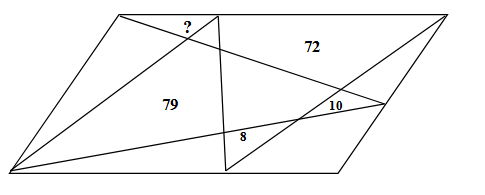
\includegraphics[scale=0.6]{06.png}}
\end{figure}\\
188. На чертеже --- параллелограмм. Подписаны площади его отдельных частей. Определите площадь четырёхугольника, отмеченного знаком вопроса.
\begin{figure}[ht!]
\center{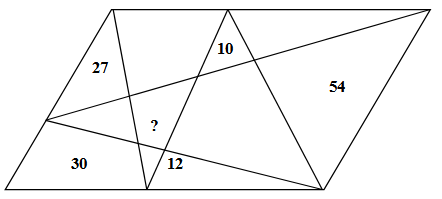
\includegraphics[scale=0.6]{07.png}}
\end{figure}\\
189. Найдите стороны параллелограмма $ABCD,$ если его периметр равен 64 см, а биссектриса острого угла $A$ делит сторону $BC$ в отношении 1:2, считая от вершины $B.$\\
190. Найдите стороны параллелограмма $ABCD,$ если его периметр равен 100 см, а биссектриса острого угла $A$ делит сторону $BC$ в отношении 2:1, считая от вершины $B.$\\
191. Найдите меньшую высоту треугольника со сторонами, равными 15см , 17см, 8см.\\
192. Найдите меньшую высоту треугольника со сторонами, равными 24см, 25см, 7см.\\
193. Разность двух оснований равнобедренной трапеции равна 3. Синус угла при ее основании равен 0,8. Найдите длину боковой стороны трапеции.\\
194. Разность двух оснований равнобедренной трапеции равна 4. Синус угла при ее основании равен 0,6. Найдите длину боковой стороны трапеции.\\
195. Две стороны равнобедренного треугольника равны равны 3 см и 7 см. Найдите третью сторону. Ответ обосновать.\\
196. Две стороны равнобедренного треугольника равны равны 2 см и 5 см. Найдите третью сторону. Ответ обосновать.\\
197. Периметр равнобедренного треугольника равен 18 см и одна из его сторон меньше другой на 6 см. Найти стороны треугольника.\\
198. Периметр равнобедренного треугольника равен 27 см и одна из его сторон меньше другой на 9 см. Найти стороны треугольника.\\
199. В равносторонний треугольник вписана окружность радиуса 4. Найти радиус описанной окружности.\\
200. В равносторонний треугольник вписана окружность радиуса 6. Найти радиус описанной окружности.\\
201. Точка $O$ --- точка пересечения медиан $AM$ и $BK$ треугольника $ABC.$ Сравните площади треугольников $AOK$ и $BOM.$ Ответ обосновать.\\
202. $ABCD$ трапеция с основаниями $AD$ и $BC.$ Точка $O$ --- точка пересечения диагоналей трапеции. Сравните площади треугольников $ABO$ и $DCO.$ Ответ обосновать.\\
203. Углы $A$ и $B$ и треугольника $ABC$ равны соответственно $71^\circ$ и $79^\circ.$ Найдите $AB,$ если радиус окружности, описанной около треугольника $ABC,$ равен 8.\\
204. Углы $B$ и $C$ и треугольника $ABC$ равны соответственно $81^\circ$ и $69^\circ.$ Найдите $BC,$ если радиус окружности, описанной около треугольника $ABC,$ равен 5.\\
205. В равнобедренной трапеции диагональ делит тупой угол пополам. Найдите большее основание трапеции, если его длина на 25 см меньше периметра, а средняя линия равна 8 см.\\
206. В равнобедренной трапеции диагональ делит тупой угол пополам. Найдите большее основание трапеции, если его длина на 31 см меньше периметра, а средняя линия равна 10 см.\\
207. В прямоугольном треугольнике $ABC$ (угол $C$ прямой) $tg\; A=2.$ Найти $\cfrac{\sin A -\cos A}{\sin A +\cos A}.$\\
208. В прямоугольном треугольнике $ABC$ (угол $C$ прямой) $tg\; A=3.$ Найти $\cfrac{\sin A +\cos A}{\sin A - \cos A}.$\\
209. В параллелограмме $ABCD$ на продолжении стороны $DC$ взята точка $M$ так, что $DM=3DC.$ (Точка $C$
лежит между $D$и $M).\ K$ --- точка пересечения прямых $AM$ и $BC.$ Найдите площадь треугольника $ABK,$ если
площадь параллелограмма равна 12.\\
210. В параллелограмме $ABCD$ на продолжении стороны $DC$ взята точка $M$ так, что $DM=4DC.$ (Точка $C$
лежит между $D$и $M).\ K$ --- точка пересечения прямых $AM$ и $BC.$ Найдите площадь треугольника $ABK,$ если
площадь параллелограмма равна 16.\\
211. В треугольнике $ABC$ угол $B$ равен $80^\circ.\ M$ --- точка пересечения биссектрис углов $A$ и $C.$
Найдите угол между биссектрисами треугольника.\\
212. В треугольнике $ABC$ угол $B$ равен $100^\circ.\ M$ --- точка пересечения биссектрис углов $A$ и $C.$
Найдите угол между биссектрисами треугольника.\\
213. Две стороны треугольника равны 2 и 4. Какие значения может принимать третья сторона, если её длина --- целое число?\\
214. Две стороны треугольника равны 2 и 5. Какие значения может принимать третья сторона, если её длина --- целое число?\\
215. Периметр параллелограмма равен 70 см, а его высоты 3 см и 4 см. Найдите стороны параллелограмма.\\
216. Стороны параллелограмма равны 15 см и 30 см, расстояние между меньшими сторонами --- 20 см. Найдите расстояние между большими сторонами параллелограмма.\\
217. Найдите площадь параллелограмма $ABCD,$ в котором угол $A$ равен $60^\circ,$ а биссектриса $AE$ делит сторону $BC$ на отрезки $BE=2$ и $EC=1.$\\
218. Найдите площадь параллелограмма $ABCD,$ в котором угол $A$ равен $60^\circ,$ а биссектриса $AE$ делит сторону $BC$ на отрезки $BE=1$ и $EC=3.$\\
219. В треугольнике $ABC$ проведена высота $CD.$ Известно, что $CD^2=AD\cdot DB.$\\
а) Докажите, что если точка $D$ лежит на отрезке $AB,$ то треугольник $ABC$ прямоугольный.\\
б) Возможно ли такое соотношение в случае, если $D$ не лежит на отрезке $AB?$ Если да --- приведите пример, если нет --- докажите, почему.\\
220. В треугольнике $ABC$ проведена высота $CH.$ Известно, что $CH^2=AH\cdot HB.$\\
а) Докажите, что если точка $H$ лежит на отрезке $AB,$ то треугольник $ABC$ прямоугольный.\\
б) Возможно ли такое соотношение в случае, если $H$ не лежит на отрезке $AB?$ Если да --- приведите пример, если нет --- докажите, почему.\\
221. Дана равнобедренная трапеция с основаниями 1 и 3. Определить, верно или неверно утверждение (и объяснить, почему):\\
1) если высота равна 1, то диагональ больше, чем 3;\\
2) если диагональ больше, чем 3, то угол при основании больше, чем $45^\circ;$\\
3) если боковая сторона больше 2, то площадь больше 4;\\
4) если площадь равна 1, то радиус описанной окружности больше 1.\\
222. Докажите, что не существует треугольника со сторонами $\sqrt{2}$см, 4 см и $\sqrt{5}$ см.\\
223. На большем основании $AD$ трапеции $ABCD$ взята точка $N$ так, что $AN:ND=3:1.$ Найти $S(\Delta ACD),$ если $S(\Delta ABN)=6.$\\
224. Из середины каждой стороны остроугольного $\Delta ABC$ опущены перпендикуляры на две другие стороны треугольника. Найти площадь ограниченного ими шестиугольника, если $S(\Delta ABC)=8.$\\
225. В равнобедренной трапеции даны: длина меньшего основания трапеции --- $a,$ высота трапеции --- $h,$ острый угол трапеции --- $\alpha.$ Найдите периметр, среднюю линию и площадь этой трапеции.\\
226. В равнобедренной трапеции даны: длины оснований трапеции --- $a$ и $b\ (a<b),$ острый угол трапеции --- $\alpha.$ Найдите периметр, высоту и площадь этой трапеции.\\
227. На сторонах $AB$ и $AC$ треугольника $ABC$ соответственно выбрали точки $D$ и $E$ так, что $DE\parallel BC.$ Оказалось, что $AE=4,\ ED=5,\ DB=6,\ BC=20.$ Найдите периметр и площадь четырёхугольника $BDEC.$\\
228. На сторонах $AD$ и $AE$ треугольника $ADE$ соответственно выбрали точки $C$ и $B$ так, что $BC\parallel DE.$ Оказалось, что $AB=5,\ BC=6,\ CD=4,\ DE=18.$ Найдите периметр и площадь четырёхугольника $BCDE.$\\
229. Пусть $CH$ --- высота прямоугольного треугольника $ABC,$ проведённая к гипотенузе, $AH=9$см, $BC=20$см. Найдите площадь треугольника $ABC.$\\
230. Пусть $CH$ --- высота прямоугольного треугольника $ABC,$ проведённая к гипотенузе, $BH=16$см, $AC=15$см. Найдите площадь треугольника $ABC.$\\
231. На стороне $BC$ параллелограмма $ABCD$ выбрана точка $K$ так, что $BK:CK=5:2.$ Отрезок $KD$ пересекает диагональ $AC$ параллелограмма в точке $M.$ Луч $BM$ пересекает отрезок $CD$ в точке $P.$ Найдите отношение $CP:PD.$\\
232. На стороне $AD$ параллелограмма $ABCD$ выбрана точка $P$ так, что $AD:DP=4:3.$ Отрезок $PC$ пересекает диагональ $BD$ параллелограмма в точке $K.$ Луч $AK$ пересекает отрезок $CD$ в точке $M.$ Найдите отношение $CM:MD.$\\
233. Найдите периметр равнобедренного треугольника, если две его стороны равны 4 см и 9 см. Если ответов существует больше одного, в ответ запишите их сумму.\\
234. Найдите периметр равнобедренного треугольника, если две его стороны равны 5 см и 10 см. Если ответов существует больше одного, в ответ запишите их сумму.\\
235. В четырёхугольнике $ABCD$ известно, что $\angle A=90^\circ,\ \angle B=120^\circ,\ \angle D=30^\circ,\ AB=6,\ BC=4.$ Найдите $CD.$\\
236. В четырёхугольнике $ABCD$ известно, что $\angle A=90^\circ,\ \angle B=120^\circ,\ \angle D=30^\circ,\ AB=3,\ BC=2.$ Найдите $CD.$\\
237. В равнобедренной трапеции меньшее основание равно 2 см, один из углов равен $120^\circ,$ а одна из диагоналей составляет равные углы с боковой стороной и большим основанием. Найдите а) боковую сторону, б) периметр этой трапеции.\\
238. Основание равнобедренного треугольника имеет длину 10, а боковая сторона 13. Найти площадь треугольника; найти радиус окружности, вписанной в этот треугольник; найти расстояние между центром вписанной окружности и точкой пересечения медиан треугольника.\\
239. Высоты треугольника $ABC$ пересекаются в точке $H.$ Найти угол $ACB,$ если известно, что он тупой и $CH=AB.$\\
240. В треугольнике две стороны равны 13 и 15, а высота, проведённая к третьей стороне, равна 12. Найдите площадь треугольника.\\
241. В треугольнике две стороны равны 13 и 20, а высота, проведённая к третьей стороне, равна 12. Найдите площадь треугольника.\\
242. В трапеции углы, прилежащие к большему основанию, равны $45^\circ$ и $60^\circ,$ высота равна 6, а площадь равна 42. Найдите меньшее основание.\\
243. В трапеции углы, прилежащие к большему основанию, равны $45^\circ$ и $30^\circ,$ высота равна 4, а площадь равна 32. Найдите меньшее основание.\\
244. На сторонах $AB$ и $AC$ треугольника $ABC$ отмечены соответственно точки $C_1$ и $B_1$ так, что $AC_1=7,\
C_1B=2,\ AB_1=3,\ B_1C=18.$ Биссектриса угла $A$ пересекает отрезки $BC$ и $B_1C_1$ в точках $T$ и $T_1$ соответственно, причём
$TT_1=8.$ Найдите $AT_1.$\\
245. На сторонах $AB$ и $AC$ треугольника $ABC$ отмечены соответственно точки $C_1$ и $B_1$ так, что $AC_1=5,\
C_1B=23,\ AB_1=7,\ B_1C=13.$ Биссектриса угла $A$ пересекает отрезки $BC$ и $B_1C_1$ в точках $T$ и $T_1$ соответственно, причём
$TT_1=9.$ Найдите $AT_1.$\\
246. В прямоугольном треугольнике высота, проведённая к гипотенузе, равна $h,$ а один из острых
углов равен $\alpha.$ Найдите периметр треугольника.\\
247. В прямоугольном треугольнике высота, проведённая к гипотенузе, равна $h,$ а один из острых
углов равен $\alpha.$ Найдите площадь треугольника.\\
248. На окружности расположены точки $A,\ B,\ C,\ D,$ причём $\angle ADC=\angle CBA=52^\circ,\
\angle ADB=43^\circ.$ Найдите $\angle CAB.$\\
249. На окружности расположены точки $A,\ B,\ C,\ D,$ причём $\angle ADC=\angle CBA=56^\circ,\
\angle ADB=37^\circ.$ Найдите $\angle CAB.$\\
250. Найдите катеты прямоугольного треугольника, высота
которого делит гипотенузу на отрезки, один из которых
на 3 см меньше этой высоты, а другой на 4 см больше
высоты.\\
251. Перпендикуляр, опущенный из точки пересечения
диагоналей ромба на его сторону, равен 2 см и делит эту
сторону на отрезки, относящиеся как $1:4.$ Найдите
диагонали ромба.\\
252. Диагональ равнобедренной трапеции делит высоту,
проведённую из вершины тупого угла, на отрезки длиной
15 см и 12 см, а боковая сторона трапеции равна её
меньшему основанию. Найти площадь трапеции.\\
253. Большая диагональ прямоугольной трапеции делит
высоту, проведённую из вершины тупого угла, на отрезки
длиной 15 см и 9 см, а большая боковая сторона трапеции
равна её меньшему основанию. Найти площадь
трапеции.
\newpage
\section{Числовые выражения решения}
1. $\left(\cfrac{4}{3}\sqrt{3}+\sqrt{2}+\sqrt{3\frac{1}{3}}\right): \left(-\sqrt{\frac{1}{3}}\right)+\sqrt{2}(\sqrt{3}+\sqrt{5})+\cfrac{9-2\sqrt{3}}{3\sqrt{6}-2\sqrt{2}}=
\left(\cfrac{4}{3}\sqrt{3}+\sqrt{2}+\cfrac{\sqrt{10}}{\sqrt{3}}\right)\cdot(-\sqrt{3})+\sqrt{6}+\sqrt{10}+\cfrac{(9-2\sqrt{3})(3\sqrt{6}+2\sqrt{2})}{54-8}=
-4-\sqrt{6}-\sqrt{10}+\sqrt{6}+\sqrt{10}+\cfrac{27\sqrt{6}+18\sqrt{2}-18\sqrt{2}-4\sqrt{6}}{46}=\cfrac{\sqrt{6}}{2}-4.$\\
2. $\left(\cfrac{1}{4}+\sqrt{\frac{1}{5}}-2\sqrt{2}\right): \left(\cfrac{1}{2}\sqrt{\frac{1}{5}}\right)-\cfrac{1}{2}\sqrt{5}+4\sqrt{10}+\cfrac{2\sqrt{6}+3\sqrt{3}}{4+3\sqrt{2}}=
\left(\cfrac{1}{4}+\cfrac{1}{\sqrt{5}}-2\sqrt{2}\right)\cdot2\sqrt{5}-\cfrac{1}{2}\sqrt{5}+4\sqrt{10}+\cfrac{(2\sqrt{6}+3\sqrt{3})(3\sqrt{2}-4)}{18-16}=
\cfrac{1}{2}\sqrt{5}+2-4\sqrt{10}-\cfrac{1}{2}\sqrt{5}+4\sqrt{10}+\cfrac{12\sqrt{3}-8\sqrt{6}+9\sqrt{6}-12\sqrt{3}}{2}=
\cfrac{\sqrt{6}}{2}+2.$\\
3. $\sqrt{9+4\sqrt{5}}-\sqrt{6-2\sqrt{5}}=\sqrt{2^2+2\cdot2\cdot\sqrt{5}+(\sqrt{5})^2}-\sqrt{1^2-2\cdot1\cdot\sqrt{5}+(\sqrt{5})^2}=$\\$=
\sqrt{(2+\sqrt{5})^2}-\sqrt{(1-\sqrt{5})^2}=|2+\sqrt{5}|-|1-\sqrt{5}|=(2+\sqrt{5})-(\sqrt{5}-1)=3.$\\
4. $\sqrt{12+6\sqrt{3}}-\sqrt{4-2\sqrt{3}}=\sqrt{3^2+2\cdot3\cdot\sqrt{5}+(\sqrt{3})^2}-\sqrt{1^2-2\cdot1\cdot\sqrt{3}+(\sqrt{3})^2}=$\\$=
\sqrt{(3+\sqrt{3})^2}-\sqrt{(1-\sqrt{3})^2}=|3+\sqrt{3}|-|1-\sqrt{3}|=(3+\sqrt{3})-(\sqrt{3}-1)=4.$\\
5. $2\sqrt{8\frac{1}{2}}-\sqrt{306}+5\sqrt{1\frac{9}{25}}=2\sqrt{\frac{17}{2}}-3\sqrt{34}+5\sqrt{\frac{34}{25}}=
\sqrt{34}-3\sqrt{34}+\sqrt{34}=-\sqrt{34}.$\\
6. $4\sqrt{10\frac{1}{2}}+\sqrt{168}-15\sqrt{1\frac{17}{25}}=4\sqrt{\frac{21}{2}}+2\sqrt{42}-15\sqrt{\frac{42}{25}}=
2\sqrt{42}+2\sqrt{42}-3\sqrt{42}=\sqrt{42}.$\\
7. $\sqrt{7+4\sqrt{3}}+\sqrt{7-4\sqrt{3}}=\sqrt{2^2+2\cdot2\cdot\sqrt{3}+(\sqrt{3})^2}+\sqrt{2^2-2\cdot2\cdot\sqrt{3}+(\sqrt{3})^2}=
|2+\sqrt{3}|+|2-\sqrt{3}|=2+\sqrt{3}+2-\sqrt{3}=4.$\\
8. $\sqrt{8+2\sqrt{7}}+\sqrt{8-2\sqrt{7}}==\sqrt{1^2+2\cdot1\cdot\sqrt{7}+(\sqrt{7})^2}+\sqrt{1^2-2\cdot1\cdot\sqrt{7}+(\sqrt{7})^2}=
|1+\sqrt{7}|+|1-\sqrt{7}|=1+\sqrt{7}+\sqrt{7}-1=2\sqrt{7}.$\\
9. $\cfrac{1}{\sqrt{6-\sqrt{20}}+1}-\cfrac{1}{\sqrt{6+\sqrt{20}}-1}=\cfrac{1}{\sqrt{1^2-2\cdot1\cdot\sqrt{5}+(\sqrt{5})^2}+1}-\cfrac{1}{\sqrt{1^2+2\cdot1\cdot\sqrt{5}+(\sqrt{5})^2}-1}=
\cfrac{1}{\sqrt{(1-\sqrt{5})^2}+1}-\cfrac{1}{\sqrt{(1+\sqrt{5})^2}-1}=\cfrac{1}{\sqrt{5}-1+1}-\cfrac{1}{\sqrt{5}+1-1}=
\cfrac{1}{\sqrt{5}}-\cfrac{1}{\sqrt{5}}=0.$\\
10. $\cfrac{1}{\sqrt{4-\sqrt{12}}+1}-\cfrac{1}{\sqrt{4+\sqrt{12}}-1}=\cfrac{1}{\sqrt{1^2-2\cdot1\cdot\sqrt{3}+(\sqrt{3})^2}+1}-\cfrac{1}{\sqrt{1^2+2\cdot1\cdot\sqrt{3}+(\sqrt{3})^2}-1}=
\cfrac{1}{\sqrt{(1-\sqrt{3})^2}+1}-\cfrac{1}{\sqrt{(1+\sqrt{3})^2}-1}=\cfrac{1}{\sqrt{3}-1+1}-\cfrac{1}{\sqrt{3}+1-1}=
\cfrac{1}{\sqrt{3}}-\cfrac{1}{\sqrt{3}}=0.$\\
11. $\cfrac{\left(\cfrac{1}{4}-\cfrac{5}{24}\right)\cdot 8-\cfrac{1}{3}}{1,85-1,62:0,9}=
\cfrac{\cfrac{1}{24}\cdot 8-\cfrac{1}{3}}{1,85-1,62:0,9}=\cfrac{0}{1,85-1,62:0,9}=0.$\\
12. $\cfrac{\left(1\cfrac{2}{9}:7\cfrac{1}{3}-\cfrac{1}{6}\right)\cdot0,23}{2\cfrac{1}{8}+\cfrac{1}{2}}=
\cfrac{\left(\cfrac{11}{9}\cdot\cfrac{3}{22}-\cfrac{1}{6}\right)\cdot0,23}{2\cfrac{1}{8}+\cfrac{1}{2}}=
\cfrac{0\cdot0,23}{2\cfrac{1}{8}+\cfrac{1}{2}}=0.$\\
13. $\sqrt{28-10\sqrt{3}}+\sqrt{28+10\sqrt{3}}=\sqrt{5^2-2\cdot5\cdot\sqrt{3}+(\sqrt{3})^2}+\sqrt{5^2+2\cdot5\cdot\sqrt{3}+(\sqrt{3})^2}=\sqrt{(5-\sqrt{3})^2}+
\sqrt{(5+\sqrt{3})^2}=|5-\sqrt{3}|+|5+\sqrt{3}|=5-\sqrt{3}+5+\sqrt{3}=10.$\\
14. $\sqrt{14+6\sqrt{5}}+\sqrt{14-6\sqrt{5}}=\sqrt{3^2+2\cdot3\cdot\sqrt{5}+(\sqrt{5})^2}+\sqrt{3^2-2\cdot3\cdot\sqrt{5}+(\sqrt{5})^2}=\sqrt{(3+\sqrt{5})^2}+
\sqrt{(3-\sqrt{5})^2}=|3+\sqrt{5}|+|3-\sqrt{5}|=3+\sqrt{5}+3-\sqrt{5}=6.$\\
15. Пусть $3458\cfrac{239}{9876}=x,$ тогда искомое выражение равно $x(x-1)-(x+1)(x-2)=x^2-x-x^2+2x-x+2=2.$\\
16. Пусть $4357\cfrac{239}{9876}=x,$ тогда искомое выражение равно $(x+2)(x-1)-(x+1)x=x^2-x+2x-2-x^2-x=-2.$\\
17. $\sqrt{6+2\sqrt{5}}-\sqrt{6-2\sqrt{5}}=\sqrt{1^2+2\cdot1\cdot\sqrt{5}+(\sqrt{5})^2}-\sqrt{1^2-2\cdot1\cdot\sqrt{5}+(\sqrt{5})^2}=\sqrt{(1+\sqrt{5})^2}-
\sqrt{(1-\sqrt{5})^2}=|1+\sqrt{5}|-|1-\sqrt{5}|=1+\sqrt{5}-\sqrt{5}+1=2.$\\
18. $\sqrt{7+2\sqrt{6}}-\sqrt{7-2\sqrt{6}}=\sqrt{1^2+2\cdot1\cdot\sqrt{6}+(\sqrt{6})^2}-\sqrt{1^2-2\cdot1\cdot\sqrt{6}+(\sqrt{6})^2}=\sqrt{(1+\sqrt{6})^2}-
\sqrt{(1-\sqrt{6})^2}=|1+\sqrt{6}|-|1-\sqrt{6}|=1+\sqrt{6}-\sqrt{6}+1=2.$\\
19. $b=\cfrac{2}{\sqrt{7+3\sqrt{5}}}=\cfrac{2\sqrt{7-3\sqrt{5}}}{\sqrt{49-45}}=\sqrt{7-3\sqrt{5}}=a.$\\
20. $b=\cfrac{2}{\sqrt{8+2\sqrt{15}}}=\cfrac{2\sqrt{8-2\sqrt{15}}}{64-60}=\sqrt{8-2\sqrt{15}}=a.$\\
21. $\cfrac{\sqrt{2+\sqrt{3}}-\sqrt{2-\sqrt{3}}}{\sqrt{2}}=\cfrac{\sqrt{4+2\sqrt{3}}-\sqrt{4-2\sqrt{3}}}{2}=$\\$=
\cfrac{\sqrt{1^2+2\cdot1\cdot\sqrt{3}+(\sqrt{3})^2}-\sqrt{1^2-2\cdot1\cdot\sqrt{3}+(\sqrt{3})^2}}{2}=
\cfrac{\sqrt{(1+\sqrt{3})^2}-\sqrt{(1-\sqrt{3})^2}}{2}=$\\$=\cfrac{1+\sqrt{3}-\sqrt{3}+1}{2}=1.$\\
22. $\cfrac{\sqrt{3+\sqrt{5}}-\sqrt{3-\sqrt{5}}}{\sqrt{2}}=\cfrac{\sqrt{6+2\sqrt{5}}-\sqrt{6-2\sqrt{5}}}{2}=$\\$=
\cfrac{\sqrt{1^2+2\cdot1\cdot\sqrt{5}+(\sqrt{5})^2}-\sqrt{1^2-2\cdot1\cdot\sqrt{5}+(\sqrt{5})^2}}{2}=
\cfrac{\sqrt{(1+\sqrt{5})^2}-\sqrt{(1-\sqrt{5})^2}}{2}=$\\$=\cfrac{1+\sqrt{5}-\sqrt{5}+1}{2}=1.$\\
23. Пусть $135=x,$ тогда искомое выражение равно $(x-4)(x+4)-(x-2)(x+2)=x^2-16-x^2+4=-12.$\\
24. Пусть $145=x,$ тогда искомое выражение равно $(x-4)(x+4)-(x-2)(x+2)=x^2-16-x^2+4=-12.$\\
25. $\sqrt{4+2\sqrt{3}}-\sqrt{4-2\sqrt{3}}=\sqrt{1^2+2\cdot1\cdot\sqrt{3}+(\sqrt{3})^2}-\sqrt{1^2-2\cdot1\cdot\sqrt{3}+(\sqrt{3})^2}=
\sqrt{(1+\sqrt{3})^2}-\sqrt{(1-\sqrt{3})^2}=1+\sqrt{3}-\sqrt{3}+1=2.$\\
26. $\sqrt{16+2\sqrt{15}}-\sqrt{16-2\sqrt{15}}=\sqrt{1^2+2\cdot1\cdot\sqrt{15}+(\sqrt{15})^2}-\sqrt{1^2-2\cdot1\cdot\sqrt{15}+(\sqrt{15})^2}=$\\$
\sqrt{(1+\sqrt{15})^2}-\sqrt{(1-\sqrt{15})^2}=1+\sqrt{15}-\sqrt{15}+1=2.$\\
27. Пусть $5379=x,$ тогда искомое выражение равно $x^2-(x-1)(x+1)=x^2-x^2+1=1.$\\
28. Пусть $9551=x,$ тогда искомое выражение равно $(x+1)(x-1)-x^2=x^2-1-x^2=-1.$\\
29. $\sqrt{27+10\sqrt{2}}-\sqrt{2}=\sqrt{5^2+2\cdot5\cdot\sqrt{2}+(\sqrt{2})^2}-\sqrt{2}=\sqrt{(5+\sqrt{2})^2}-\sqrt{2}=
5+\sqrt{2}-\sqrt{2}=5.$\\
30. $\sqrt{21-8\sqrt{5}}+\sqrt{5}=\sqrt{4^2-2\cdot4\cdot\sqrt{2}+(\sqrt{5})^2}+\sqrt{5}=\sqrt{(4-\sqrt{5})^2}+\sqrt{5}=
4-\sqrt{5}+\sqrt{5}=4.$\\
31. $\cfrac{5,1}{0,017}+\cfrac{0,09}{0,003}+\cfrac{1}{0,1}=300+30+10=340.$\\
32. $\cfrac{2,4}{0,08}+\cfrac{0,21}{0,07}+\cfrac{4}{0,4}=30+3+10=43.$\\
33. $4+2\sqrt{2}\ ??\ \sqrt{11}+\sqrt{13},\ 16+16\sqrt{2}+8\ ??\ 11+2\sqrt{11}\cdot\sqrt{13}+13,\ 8\sqrt{2}\ ??\ \sqrt{143},\ 128<143.$\\
34. $3+2\sqrt{5}\ ??\ \sqrt{14}+\sqrt{15},\ 9+12\sqrt{5}+20\ ??\ 14+2\sqrt{14}\cdot\sqrt{15}+15,\ 6\sqrt{5}\ ??\ \sqrt{210},\ 180<210.$\\
35. $\cfrac{\sqrt{52}}{\sqrt{\sqrt{17}+2}\sqrt{\sqrt{17}-2}}=\cfrac{\sqrt{52}}{\sqrt{17-4}}=\sqrt{4}=2.$\\
36. Пусть $566=x,$ тогда искомое выражение равно $(x-4)(x+4)-(x+2)(x-2)=x^2-16-x^2+4=-12.$\\
37. $\cfrac{15^{n+4}}{3^{n+2}\cdot5^{n+3}}=\cfrac{3^{n+4}\cdot5^{n+4}}{3^{n+2}\cdot5^{n+3}}=3^2\cdot5=45.$\\
38. $\sqrt{3}\cdot\sqrt{24}\cdot\cfrac{\sqrt{63\cdot16-72\cdot6}}{\sqrt{19^2-17^2}}=
\sqrt{72}\cdot\cfrac{\sqrt{9\cdot16\cdot(7-3)}}{\sqrt{(19-17)(19+17)}}=\sqrt{72}\cdot\cfrac{3\cdot4\cdot2}{\sqrt{2\cdot36}}=24.$\\
39. $\sqrt{2}\cdot\sqrt{18}\cdot\cfrac{\sqrt{36\cdot92-48\cdot9}}{\sqrt{21^2-19^2}}=
\sqrt{36}\cdot\cfrac{\sqrt{36\cdot(92-12)}}{\sqrt{(21-19)(21+19)}}=6\cdot\cfrac{6\sqrt{80}}{\sqrt{80}}=36.$\\
40. $\sqrt{7}\cdot\sqrt{28}\cdot\cfrac{\sqrt{225\cdot32-72\cdot16}}{\sqrt{23^2-19^2}}=
\sqrt{196}\cdot\cfrac{\sqrt{16\cdot9\cdot(50-8)}}{\sqrt{(23-19)(23+19)}}=14\cdot\cfrac{4\cdot3\sqrt{42}}{2\sqrt{42}}=84.$\\
41. $\sqrt{5}\cdot\sqrt{45}\cdot\cfrac{\sqrt{126\cdot32+48\cdot18}}{\sqrt{19^2-15^2}}=
\sqrt{225}\cdot\cfrac{\sqrt{16\cdot9\cdot(28+6)}}{\sqrt{(19-15)(19+15)}}=
15\cdot\cfrac{4\cdot3\sqrt{34}}{2\sqrt{34}}=90.$\\
42. $\sqrt{1-2\sqrt{3}+3}+\sqrt{3}=\sqrt{1^2-2\cdot1\cdot\sqrt{3}+(\sqrt{3})^2}+\sqrt{3}=|1-\sqrt{3}|+\sqrt{3}=\sqrt{3}-1+\sqrt{3}=2\sqrt{3}-1.$\\
43. $-\sqrt{5}-\sqrt{1-2\sqrt{5}+5}=-\sqrt{5}-\sqrt{1^2-2\cdot1\cdot\sqrt{5}+(\sqrt{5})^2}=-\sqrt{5}-|1-\sqrt{5}|=-\sqrt{5}-\sqrt{5}+1=1-2\sqrt{5}.$\\
44. $-\sqrt{3}-\sqrt{1-2\sqrt{3}+3}=-\sqrt{3}-\sqrt{1^2-2\cdot1\cdot\sqrt{3}+(\sqrt{3})^2}=-\sqrt{3}-|1-\sqrt{3}|=-\sqrt{3}-\sqrt{3}+1=1-2\sqrt{3}.$\\
45. $\sqrt{5}+\sqrt{1-2\sqrt{5}+5}=\sqrt{5}+\sqrt{1^2-2\cdot1\cdot\sqrt{5}+(\sqrt{5})^2}=\sqrt{5}+|1-\sqrt{5}|=\sqrt{5}+\sqrt{5}-1=2\sqrt{5}-1.$\\
46. $\sqrt{83-18\sqrt{2}}-\sqrt{2}=\sqrt{9^2-2\cdot9\cdot\sqrt{2}+(\sqrt{2})^2}-\sqrt{2}=\sqrt{(9-\sqrt{2})^2}-\sqrt{2}=|9-\sqrt{2}|-\sqrt{2}=9-2\sqrt{2}.$\\
47. $\sqrt{54-14\sqrt{5}}+\sqrt{5}=\sqrt{7^2-2\cdot7\cdot\sqrt{5}+(\sqrt{5})^2}+\sqrt{5}=\sqrt{(7-\sqrt{5})^2}+\sqrt{5}=|7-\sqrt{5}|+\sqrt{5}=7.$\\
48. $(2-\sqrt{5})(\sqrt{9+4\sqrt{5}})=(2-\sqrt{5})\left(\sqrt{2^2+2\cdot2\cdot\sqrt{5}+(\sqrt{5})^2}\right)=(2-\sqrt{5})\left(\sqrt{(2+\sqrt{5})^2}\right)=$\\$=
(2-\sqrt{5})(2+\sqrt{5})=4-5=-1.$\\
49. $(2-\sqrt{7})(\sqrt{11+4\sqrt{7}}=(2-\sqrt{7})\left(\sqrt{2^2+2\cdot2\cdot\sqrt{7}+(\sqrt{7})^2}\right)=(2-\sqrt{7})\left(\sqrt{(2+\sqrt{7})^2}\right)=$\\$=
(2-\sqrt{7})(2+\sqrt{7})=4-7=-3.$\\
50. $\cfrac{180\cdot3,91-168+859\cdot1,8-768}{239\cfrac{5}{6}-237\cfrac{2}{3}}=
\cfrac{1,8\cdot391+859\cdot1,8-936}{2\cfrac{1}{6}}=\cfrac{1,8\cdot(391+859)-936}{\cfrac{13}{6}}=$\\$=\cfrac{2250-936}{\cfrac{13}{6}}=
(1313+1)\cdot\cfrac{6}{13}=606\cfrac{6}{13}.$\\
51. $\cfrac{1,7\cdot229-1155+7,91\cdot170+937}{366\cfrac{5}{6}-364\cfrac{29}{42}}=
\cfrac{1,7\cdot229+791\cdot1,7-218}{2\cfrac{1}{7}}=\cfrac{1,7\cdot(229+791)-218}{\cfrac{15}{7}}=$\\$=\cfrac{1734-218}{\cfrac{15}{7}}=
(1515+1)\cdot\cfrac{7}{15}=707\cfrac{7}{15}.$\\
52. $\cfrac{(8^{2020}+8^{2019})^2}{(4^{2019}-4^{2018})^3}=\cfrac{(8^{2019}\cdot(8+1))^2}{(4^{2018}\cdot(4-1))^3}=
\cfrac{8^{4038}\cdot81}{4^{6054}\cdot27}=\cfrac{2^{12114}\cdot3}{2^{12108}}=2^6\cdot3=192.$\\
53. $\cfrac{(4^{3021}-4^{3020})^3}{(8^{3020}+8^{3019})^2}=\cfrac{(4^{3020}\cdot(4-1))^3}{(8^{3019}\cdot(8+1))^2}=
\cfrac{4^{9060}\cdot27}{8^{6038}\cdot81}=\cfrac{2^{18120}}{2^{18114}\cdot3}=\cfrac{2^6}{3}=\cfrac{64}{3}.$\\
54. Пусть $30\cfrac{1}{239}=x,$ тогда искомое выражение равно $x^2-(x+1)(x-1)=x^2-x^2+1=1.$\\
55. $(2-\sqrt{5})\sqrt{18+8\sqrt{5}}=(2-\sqrt{5})\sqrt{2(2^2+2\cdot2\cdot\sqrt{5}+(\sqrt{5})^2)}=(2-\sqrt{5})\sqrt{2(2+\sqrt{5})^2}=$\\$=
(2-\sqrt{5})\cdot\sqrt{2}(2+\sqrt{5})=(4-5)\sqrt{2}=-\sqrt{2}.$\\
56. $\cfrac{1}{\sqrt{7+4\sqrt{3}}}+\cfrac{1}{\sqrt{7-4\sqrt{3}}}=\cfrac{1}{\sqrt{2^2+2\cdot2\cdot\sqrt{3}+(\sqrt{3})^2}}+\cfrac{1}{\sqrt{2^2-2\cdot2\cdot\sqrt{3}+(\sqrt{3})^2}}=$\\
$=\cfrac{1}{\sqrt{(2+\sqrt{3})^2}}+\cfrac{1}{\sqrt{(2-\sqrt{3})^2}}=\cfrac{1}{2+\sqrt{3}}+\cfrac{1}{2-\sqrt{3}}=
\cfrac{2-\sqrt{3}+2+\sqrt{3}}{4-3}=4.$\\
57.
$\cfrac{1}{\sqrt{9+4\sqrt{5}}}+\cfrac{1}{\sqrt{9-4\sqrt{5}}}=\cfrac{1}{\sqrt{2^2+2\cdot2\cdot\sqrt{5}+(\sqrt{5})^2}}+\cfrac{1}{\sqrt{2^2-2\cdot2\cdot\sqrt{5}+(\sqrt{5})^2}}=$\\
$=\cfrac{1}{\sqrt{(2+\sqrt{5})^2}}+\cfrac{1}{\sqrt{(2-\sqrt{5})^2}}=\cfrac{1}{2+\sqrt{5}}+\cfrac{1}{\sqrt{5}-2}=
\cfrac{\sqrt{5}-2+\sqrt{5}+2}{5-4}=2\sqrt{5}.$\\
58. $\cfrac{1}{\sqrt{3}-\sqrt{2}}=\cfrac{\sqrt{3}+\sqrt{2}}{3-2}=\sqrt{3}+\sqrt{2}>\sqrt{2}+\sqrt{2}=2\sqrt{2}.$\\
59. $\sqrt{10}+\sqrt{13}\ ??\ \sqrt{12}+\sqrt{11},\ 10+2\sqrt{10}\sqrt{13}+13\ ??\ 12+2\sqrt{12}\sqrt{11}+11,\ 130<132.$\\
60. $\cfrac{1}{2+\sqrt{17-12\sqrt{2}}}=\cfrac{1}{2+\sqrt{3^2-2\cdot3\cdot2\sqrt{2}+(2\sqrt{2})^2}}=
\cfrac{1}{2+\sqrt{(3-2\sqrt{2})^2}}=\cfrac{1}{2+3-2\sqrt{2}}=$\\$=\cfrac{1}{5-2\sqrt{2}}=
\cfrac{5+2\sqrt{2}}{25-8}=\cfrac{5+2\sqrt{2}}{17}<\cfrac{5+3}{17}=\cfrac{8}{17}.$ Заметим, что $3>2\sqrt{2}$ так как $9>8.$\\
61. $(4+\sqrt{15})(\sqrt{10}-\sqrt{6})\sqrt{4-\sqrt{15}}=(4+\sqrt{15})\sqrt{2}(\sqrt{5}-\sqrt{3})\sqrt{4-\sqrt{15}}=$\\$=
(4+\sqrt{15})(\sqrt{5}-\sqrt{3})\sqrt{8-2\sqrt{15}}=(4+\sqrt{15})(\sqrt{5}-\sqrt{3})\sqrt{(\sqrt{5})^2-2\sqrt{5}\sqrt{3}+(\sqrt{3})^2}=
(4+\sqrt{15})(\sqrt{5}-\sqrt{3})\sqrt{(\sqrt{5}-\sqrt{3})^2}=(4+\sqrt{15})(\sqrt{5}-\sqrt{3})^2=
(4+\sqrt{15})(5-2\sqrt{15}+3)=(4+\sqrt{15})2(4-\sqrt{15})=2(16-15)=$\\$=2.$\\
62. $\cfrac{3^2-0,363^2}{3,363}=\cfrac{(3-0,363)(3+0,363)}{3,363}=2,637.$\\
63. $\cfrac{\left(0,875-\cfrac{1}{8}\right):0,75-1}{0,125+\cfrac{7}{8}}=\cfrac{0,75:0,75-1}{0,125+\cfrac{7}{8}}=\cfrac{0}{0,125+\cfrac{7}{8}}=0.$\\
64. $\left(\sqrt{3+\sqrt{5}}+\sqrt{3-\sqrt{5}}\right)^2=3+\sqrt{5}+2\sqrt{(3+\sqrt{5})(3-\sqrt{5})}+3-\sqrt{5}=
6+2\sqrt{9-5}=6+4=10.$\\
65. Пусть $2019=x,$ тогда искомое выражение равно $\sqrt{\sqrt{(x-3)(x-1)(x+1)(x+3)+16}+5}=\sqrt{\sqrt{(x^2-9)(x^2-1)+16}+5}=
\sqrt{\sqrt{x^4-9x^2-x^2+9+16}+5}=\sqrt{\sqrt{x^4-10x^2+25}+5}=$\\$=\sqrt{\sqrt{(x^2-5)^2}+5}=\sqrt{x^2-5+5}=x=2019.$\\
66. Пусть $2017=x,$ тогда искомое выражение равно $\sqrt{\sqrt{(x-4)(x-2)(x+2)(x+4)+36}+10}=\sqrt{\sqrt{(x^2-16)(x^2-4)+36}+10}=
\sqrt{\sqrt{x^4-16x^2-4x^2+64+36}+10}=\sqrt{\sqrt{x^4-20x^2+100}+10}=$\\$=\sqrt{\sqrt{(x^2-10)^2}+10}=\sqrt{x^2-10+10}=x=2017.$\\
67. $\left(\cfrac{1}{2+\sqrt{3}}-\cfrac{1}{2-\sqrt{3}}\right)(\sqrt{12}-\sqrt{75})=\cfrac{2-\sqrt{3}-2-\sqrt{3}}{4-3}\cdot(2\sqrt{3}-5\sqrt{3})=
-2\sqrt{3}\cdot(-3\sqrt{3})=18.$\\
68. $\left(\cfrac{1}{3+\sqrt{5}}-\cfrac{1}{3-\sqrt{5}}\right)(\sqrt{5}+\sqrt{45})=\cfrac{3-\sqrt{5}-3-\sqrt{5}}{9-5}\cdot(\sqrt{5}+3\sqrt{5})=
\cfrac{-2\sqrt{5}}{4}\cdot4\sqrt{5}=-10.$\\
69. $\sqrt{(\sqrt{2}-3)^2}+\sqrt{27+10\sqrt{2}}=|\sqrt{2}-3|+\sqrt{5^2+2\cdot5\cdot\sqrt{2}+(\sqrt{2})^2}=
3-\sqrt{2}+\sqrt{(5+\sqrt{2})^2}=3-\sqrt{2}+5+\sqrt{2}=8.$\\
70. $\cfrac{\left(0,5:1,25+\cfrac{7}{5}:1\cfrac{4}{7}-\cfrac{3}{11}\right)\cdot3}{\left(1,5+\cfrac{1}{4}\right):18\cfrac{1}{3}}=
\cfrac{\left(\cfrac{2}{5}+\cfrac{49}{55}-\cfrac{3}{11}\right)\cdot3}{\cfrac{7}{4}:\cfrac{55}{3}}=
\cfrac{\cfrac{56}{55}\cdot3}{\cfrac{21}{220}}=\cfrac{56\cdot3\cdot220}{55\cdot21}=32.$\\
71. $\left(\cfrac{(2,7-0,8)\cdot2\cfrac{1}{3}}{(5,2-1,4):\cfrac{3}{70}}+0,125\right):2\cfrac{1}{2}+0,43=
\left(\cfrac{\cfrac{19}{10}\cdot\cfrac{7}{3}}{\cfrac{38}{10}\cdot\cfrac{70}{3}}+\cfrac{1}{8}\right):\cfrac{5}{2}+0,43=
\left(\cfrac{\cfrac{19\cdot7}{30}}{\cfrac{38\cdot70}{30}}+\cfrac{1}{8}\right)\cdot\cfrac{2}{5}+0,43=
\left(\cfrac{1}{20}+\cfrac{1}{8}\right)\cdot\cfrac{2}{5}+0,43=\cfrac{7}{40}\cdot\cfrac{2}{5}+0,43=0,07+0,43=\cfrac{1}{2}.$\\
72. $\left(\cfrac{1}{2}\sqrt{6}-3\sqrt{3}+5\sqrt{2}-\sqrt{8}\right)\cdot\sqrt{24}+18\sqrt{2}-12\sqrt{3}=
\cfrac{1}{2}\sqrt{144}-3\sqrt{72}+5\sqrt{48}-\sqrt{192}+18\sqrt{2}-12\sqrt{3}=
\cfrac{1}{2}\cdot12-18\sqrt{2}+20\sqrt{3}-8\sqrt{3}+18\sqrt{2}-12\sqrt{3}=6.$\\
73. $\left(\cfrac{1}{2}\sqrt{32}-\cfrac{1}{3}\sqrt{3}+4\sqrt{15}-\sqrt{8}\right)\cdot\sqrt{12}-4\sqrt{6}-24\sqrt{5}=
\cfrac{1}{2}\sqrt{384}-\cfrac{1}{3}\sqrt{36}+4\sqrt{180}-\sqrt{96}-4\sqrt{6}-24\sqrt{5}=
\cfrac{1}{2}\cdot8\sqrt{6}-2+24\sqrt{5}-4\sqrt{6}-4\sqrt{6}-24\sqrt{5}=-2-4\sqrt{6}.$\\
74. $\sqrt{7+4\sqrt{3}}+\sqrt{7-4\sqrt{3}}=\sqrt{2^2+2\cdot2\sqrt{3}+(\sqrt{3})^2}+\sqrt{2^2-2\cdot2\sqrt{3}+(\sqrt{3})^2}=|2+\sqrt{3}|+|2-\sqrt{3}|=
2+\sqrt{3}+2-\sqrt{3}=4.$\\
75. $\sqrt{8+2\sqrt{7}}-\sqrt{8-2\sqrt{7}}=\sqrt{1^2+2\cdot1\sqrt{7}+(\sqrt{7})^2}+\sqrt{1^2-2\cdot1\sqrt{7}+(\sqrt{7})^2}=|1+\sqrt{7}|+|1-\sqrt{7}|=
1+\sqrt{7}+1-\sqrt{7}=2.$\\
76. $2\sqrt{9\cfrac{1}{2}}-\sqrt{342}+5\sqrt{1\cfrac{13}{25}}=2\sqrt{\cfrac{19}{2}}-3\sqrt{38}+5\sqrt{\cfrac{38}{25}}=\sqrt{38}-3\sqrt{38}+\sqrt{38}=-\sqrt{38}.$\\
77. $\cfrac{2^{19}\cdot27^3+15\cdot4^9\cdot9^4}{6^9\cdot2^{10}+12^{10}}=\cfrac{2^{19}\cdot3^9+3\cdot5\cdot2^{18}\cdot3^8}{2^9\cdot3^9\cdot2^{10}+2^{20}\cdot3^{10}}=
\cfrac{2^{18}\cdot3^9\cdot(2+5)}{2^{19}\cdot3^9\cdot(1+2\cdot3)}=\cfrac{1}{2}.$\\
78. $\cfrac{4^{15}\cdot9^9-4\cdot3^{20}\cdot8^9}{2^9\cdot6^{19}-5\cdot2^{29}\cdot27^6}=
\cfrac{2^{30}\cdot3^{18}-2^2\cdot3^{20}\cdot2^{27}}{2^9\cdot2^{19}\cdot3^{19}-5\cdot2^{29}\cdot3^{18}}=
\cfrac{2^{29}\cdot3^{18}\cdot(2-3^2)}{2^{28}\cdot3^{18}\cdot(3-5\cdot2)}=2.$\\
79. $\left(\cfrac{1}{2}\sqrt{6}-\sqrt{12}+0,5\sqrt{24}+\cfrac{3\sqrt{48}}{4}\right)\cdot2\sqrt{2}=
\left(\cfrac{1}{2}\sqrt{6}-2\sqrt{3}+\sqrt{6}+\cfrac{12\sqrt{3}}{4}\right)\cdot2\sqrt{2}=
\left(\cfrac{3}{2}\sqrt{6}+\sqrt{3}\right)\cdot2\sqrt{2}=6\sqrt{3}+2\sqrt{6}.$\\
80. $(8\sqrt{24}-12\sqrt{54}+6\sqrt{96}-4\sqrt{150}):2\sqrt{3}=
(16\sqrt{6}-36\sqrt{6}+24\sqrt{6}-20\sqrt{6}):2\sqrt{3}=(-16\sqrt{6}):2\sqrt{3}=-8\sqrt{2}.$\\
81. $\sqrt{5-\sqrt{24}}+\sqrt{5+\sqrt{24}}=\sqrt{3-2\sqrt{6}+2}+\sqrt{3+2\sqrt{6}+2}=\sqrt{(\sqrt{3}-\sqrt{2})^2}+\sqrt{(\sqrt{3}+\sqrt{2})^2}=
\sqrt{3}-\sqrt{2}+\sqrt{3}+\sqrt{2}=2\sqrt{3}.$ Так как $3^2=9<12=(2\sqrt{3})^2<16=4^2,$ данное число лежит в промежутке $(3;4).$\\
82. $\cfrac{17\sqrt{3}}{3\sqrt{5}-7\sqrt{3}}-\cfrac{3\sqrt{5}-\sqrt{3}}{5\sqrt{3}-4\sqrt{5}}=
\cfrac{17\sqrt{3}(3\sqrt{5}+7\sqrt{3})}{45-147}-\cfrac{(3\sqrt{5}-\sqrt{3})(5\sqrt{3}+4\sqrt{5})}{75-80}=$\\$
\cfrac{51\sqrt{15}+357}{-102}-\cfrac{15\sqrt{15}+60-15-4\sqrt{15}}{-5}=
\cfrac{-7-\sqrt{15}}{2}+\cfrac{11\sqrt{15}+45}{5}=\cfrac{11}{2}+\cfrac{17\sqrt{15}}{10}.$\\
83. $\cfrac{2\sqrt{5}-\sqrt{3}}{5\sqrt{3}-4\sqrt{5}}-\cfrac{21\sqrt{5}}{4\sqrt{5}-6\sqrt{3}}=
\cfrac{(2\sqrt{5}-\sqrt{3})(5\sqrt{3}+4\sqrt{5})}{5\sqrt{3}-4\sqrt{5}}-\cfrac{21\sqrt{5}(4\sqrt{5}+6\sqrt{3})}{4\sqrt{5}-6\sqrt{3}}=$\\$
\cfrac{10\sqrt{15}+40-15-4\sqrt{15}}{75-80}-\cfrac{420+126\sqrt{15}}{80-108}=
\cfrac{6\sqrt{15}+25}{-5}-\cfrac{420+126\sqrt{15}}{-28}=
-\cfrac{6\sqrt{15}+25}{5}+\cfrac{30+9\sqrt{15}}{2}=10+\cfrac{33\sqrt{15}}{10}.$\\
84. $(\sqrt{10}-\sqrt{5})\cdot\sqrt{\cfrac{20}{(1-\sqrt{2})^2}}=\sqrt{5}(\sqrt{2}-1)\cdot\cfrac{2\sqrt{5}}{\sqrt{2}-1}=10>9,99.$\\
85. $(\sqrt{8}+\sqrt{10})\cdot\sqrt{32\cdot(2-\sqrt{5})^2}=\sqrt{2}(2+\sqrt{5})\cdot4\sqrt{2}(\sqrt{5}-2)=8\cdot(5-4)=8>7,99.$\\
86. $\cfrac{\left(5\cfrac{7}{30}-3\cfrac{5}{18}\right):2\cfrac{2}{3}}{(1,2)^2-1,26:0,9}=
\cfrac{\cfrac{88}{45}\cdot\cfrac{3}{8}}{1,44-1,4}=\cfrac{\cfrac{11}{15}}{0,04}=\cfrac{55}{3}.$ Тогда искомое число равно
$\cfrac{55}{3}:36\cfrac{2}{3}\cdot100=\cfrac{55}{3}:\cfrac{110}{3}\cdot100=50.$\\
87. $\cfrac{18^{n+3}}{3^{2n+5}\cdot2^{n+2}}=\cfrac{2^{n+3}\cdot3^{2n+6}}{3^{2n+5}\cdot2^{n+2}}=2\cdot3=6.$\\
88. $\left(\cfrac{76^2+44^2+2\cdot44\cdot76}{120}\right):(37^2-13^2)=\cfrac{(76+44)^2}{120}:((37-13)(37+13))=\cfrac{120^2}{120}:(24\cdot50)=\cfrac{120}{1200}=\cfrac{1}{10}.$\\
89. $4322^2-4321\cdot4323=4322^2-(4322-1)(4322+1)=4322^2-(4322^2-1)=1.$\\
90. $\sqrt{9-4\sqrt{5}}-\cfrac{4}{\sqrt{5}+1}=\sqrt{(\sqrt{5}-2)^2}-\cfrac{4(\sqrt{5}-1)}{5-1}=
\sqrt{5}-2-(\sqrt{5}-1)=-1.$\\
91. $\sqrt{48}+\sqrt{11}\ ??\ \sqrt{27}+5,\ 4\sqrt{3}+\sqrt{11}\ ??\ 3\sqrt{3}+5,\ \sqrt{3}+\sqrt{11}\ ??\ 5,\ 3+2\sqrt{33}+11\ ??\ 25,\
2\sqrt{33}\ ??\ 11,\ 132>121.$\\
92. $\sqrt{8}+5\ ??\ \sqrt{18}+\sqrt{13},\ 8+10\sqrt{8}+25\ ??\ 18+2\sqrt{234}+13,\ 20\sqrt{2}+2\ ??\ 2\sqrt{234},\ 10\sqrt{2}+1\ ??\ \sqrt{234},\ 200+20\sqrt{2}+1\ ??\ 234,\ 20\sqrt{2}\ ??\ 33,\ 800<1089.$\\
93. $\sqrt{(2\sqrt{2}-3)^2}-\cfrac{8}{4+2\sqrt{2}}=[(2\sqrt{2})^2=8<9=3^2]=3-2\sqrt{2}-\cfrac{8(4-2\sqrt{2})}{16-8}=
3-2\sqrt{2}-4+2\sqrt{2}=-1.$\\
94. $\sqrt{(\sqrt{17}-3\sqrt{2})^2}+\cfrac{1}{\sqrt{17}-4}-3\sqrt{2}=[(\sqrt{17})^2=17<18=(3\sqrt{2})^2]=3\sqrt{2}-\sqrt{17}+\cfrac{\sqrt{17}+4}{17-16}-3\sqrt{2}=
3\sqrt{2}-\sqrt{17}+\sqrt{17}+4-3\sqrt{2}=4.$
\newpage
\section{Преобразование буквенных выражений решения}
1. $\sqrt{4x^2-4x+1}+\sqrt{16x^2-8x+1}=\sqrt{(2x-1)^2}+\sqrt{(4x-1)^2}=|2x-1|+|4x-1|=1-2x+4x-1=2x.$\\
2. $\sqrt{25x^2+10x+1}+\sqrt{9x^2+6x+1}=\sqrt{(5x+1)^2}+\sqrt{(3x+1)^2}=|5x+1|+|3x+1|=-5x-1+3x+1=-2x.$\\
3. $\cfrac{(5a-4)^2+2(5a-4)(4-3a)+(3a-4)^2}{(2a+5)^2-2(2a+5)(5-3a)+(3a-5)^2}=
\cfrac{(5a-4+4-3a)^2}{(2a+5-5+3a)^2}=\cfrac{4a^2}{25a^2}=\cfrac{4}{25}.$\\
4. $\cfrac{(4b-5)^2+2(4b-5)(5-b)+(b-5)^2}{(7b+4)^2-2(7b+4)(4-3b)+(3b-4)^2}=
\cfrac{(4b-5+5-b)^2}{(7b+4-4+3b)^2}=\cfrac{9b^2}{100b^2}=\cfrac{9}{100}.$\\
5. $\cfrac{a-b}{a-3\sqrt{ab}+2b}=[x=\sqrt{a},\ y=\sqrt{b}]=\cfrac{x^2-y^2}{x^2-3xy+2y^2}=\cfrac{(x-y)(x+y)}{x(x-y)-2y(x-y)}=\cfrac{x+y}{x-2y}=\cfrac{\sqrt{a}+\sqrt{b}}{\sqrt{a}-2\sqrt{b}}.$\\
6. $\cfrac{x+4\sqrt{xy}+3y}{x-y}=[a=\sqrt{x},\ b=\sqrt{y}]=\cfrac{a^2+4ab+3b^2}{a^2-b^2}=\cfrac{a(a+b)+3b(a+b)}{(a-b)(a+b)}=\cfrac{a+3b}{a-b}=
\cfrac{\sqrt{x}+3\sqrt{y}}{\sqrt{x}-\sqrt{y}}.$\\
7. $\cfrac{x^4-2x^3+x-2}{x^3-3x^2+3x-2}=\cfrac{x^3(x-2)+x-2}{x^3-3x^2+3x-1-1}=\cfrac{(x^3+1)(x-2)}{(x-1)^3-1}=
\cfrac{(x+1)(x^2-x+1)(x-2)}{(x-2)(x^2-2x+1+x-1+1)}=x+1.$\\
8. $\cfrac{x^6+x^4-x^2-1}{x^3+x^2+x+1}=\cfrac{x^4(x^2+1)-(x^2+1)}{x^2(x+1)+x+1}=\cfrac{(x^2+1)(x^4-1)}{(x^2+1)(x+1)}=\cfrac{(x^2-1)(x^2+1)}{x+1}=$\\$=
\cfrac{(x-1)(x+1)(x^2+1)}{x+1}=(x-1)(x^2+1).$\\
9. $\left(\cfrac{\sqrt{a}+1}{\sqrt{a}-1}-\cfrac{\sqrt{a}-1}{\sqrt{a}+1}+4\sqrt{a}\right)\cdot
\left(\sqrt{\cfrac{a}{4}}-\sqrt{\cfrac{1}{4a}}\right)=[x=\sqrt{a}]=
\left(\cfrac{x+1}{x-1}-\cfrac{x-1}{x+1}+4x\right)\cdot
\left(\cfrac{x}{2}-\cfrac{1}{2x}\right)=$\\
$=\cfrac{x^2+2x+1-x^2+2x-1+4x^3-4x}{(x-1)(x+1)}\cdot\cfrac{x^2-1}{2x}=2x^2=2a.$\\
10. $\left(\cfrac{\sqrt{a}}{\sqrt{a}+\sqrt{b}}+\cfrac{\sqrt{b}}{\sqrt{a}-\sqrt{b}}+
\cfrac{2\sqrt{ab}}{a-b}\right)\cdot\left(\sqrt{a}-\cfrac{\sqrt{ab}+b}{\sqrt{a}+\sqrt{b}}\right)=[x=\sqrt{a},\ y=\sqrt{b}]=$\\$=
\left(\cfrac{x}{x+y}+\cfrac{y}{x-y}+
\cfrac{2xy}{x^2-y^2}\right)\cdot\left(x-\cfrac{xy+y^2}{x+y}\right)=\cfrac{x^2-xy+xy+y^2+2xy}{(x-y)(x+y)}\cdot\left(x-\cfrac{y(x+y)}{x+y}\right)=$\\$=
\cfrac{x^2-xy+xy+y^2+2xy}{(x-y)(x+y)}\cdot(x-y)=\cfrac{x^2+2xy+y^2}{x+y}=\cfrac{(x+y)^2}{x+y}=x+y=\sqrt{a}+\sqrt{b}.$\\
11. $a^3-7a+6=a(a^2-1)-6(a-1)=a(a-1)(a+1)-6(a-1)=(a-1)(a^2+a-6)=(a-1)(a^2-4+a-2)=(a-1)((a-2)(a+2)+a-2)=(a-1)(a-2)(a+3).$\\
12. $a^3-7a-6=a(a^2-1)-6(a+1)=a(a-1)(a+1)-6(a+1)=(a+1)(a^2-a-6)=(a-1)(a^2-4-(a+2))=(a+1)((a-2)(a+2)-(a+2))=(a+1)(a+2)(a-3).$\\
13. $\cfrac{a^4+4}{(a+1)^2+1}=\cfrac{a^4+4a^2+4-4a^2}{a^2+2a+1+1}=\cfrac{(a^2+2)^2-(2a)^2}{a^2+2a+2}=\cfrac{(a^2-2a+2)(a^2+2a+2)}{a^2+2a+2}=a^2-2a+2.$\\
14. $\cfrac{b^4+64}{(b-2)^2+4}=\cfrac{b^4+16b^2+64-16b^2}{b^2-4b+4+4}=\cfrac{(b^2+8)^2-(4b)^2}{b^2-4b+8}=\cfrac{(b^2-4b+8)(b^2+4b+8)}{b^2-4b+8}=b^2+4b+8.$\\
15. $\left(\sqrt{a}+\cfrac{b}{\sqrt{a}-\sqrt{b}}\right)\cdot\left(1-\cfrac{\sqrt{b^3}}{a\sqrt{a}+b\sqrt{b}}\right)\cdot
(\sqrt{a}+\sqrt{b})=[x=\sqrt{a},\ y=\sqrt{b}]=$\\$=\left(x+\cfrac{y^2}{x-y}\right)\cdot\left(1-\cfrac{y^3}{x^3+y^3}\right)\cdot(x+y)=
\cfrac{x^2-xy+y^2}{x-y}\cdot\cfrac{x^3+y^3-y^3}{(x+y)(x^2-xy+y^2)}\cdot(x+y)=\cfrac{x^3}{x-y}=\cfrac{a\sqrt{a}}{\sqrt{a}-\sqrt{b}}.$\\
16. $\left(\sqrt{a}+\cfrac{b}{\sqrt{a}+\sqrt{b}}\right)\cdot\left(1+\cfrac{\sqrt{b^3}}{a\sqrt{a}-b\sqrt{b}}\right)\cdot
(\sqrt{a}-\sqrt{b})=[x=\sqrt{a},\ y=\sqrt{b}]=$\\$=\left(x+\cfrac{y^2}{x+y}\right)\cdot\left(1+\cfrac{y^3}{x^3-y^3}\right)\cdot
(x-y)=\cfrac{x^2+xy+y^2}{x+y}\cdot\cfrac{x^3-y^3+y^3}{(x-y)(x^2+xy+y^2)}\cdot(x-y)=\cfrac{x^3}{x+y}=\cfrac{a\sqrt{a}}{\sqrt{a}-\sqrt{b}}.$\\
17. $\cfrac{a+1}{a^4+a^3+a^2}: \cfrac{1}{a^5-a^2}=\cfrac{a+1}{a^2(a^2+a+1)}\cdot\cfrac{a^2(a-1)(a^2+a+1)}{1}=a^2-1.$\\
18. $\cfrac{a-1}{a^4-a^3+a^2}: \cfrac{1}{a^5+a^2}=\cfrac{a-1}{a^2(a^2-a+1)}\cdot\cfrac{a^2(a+1)(a^2-a+1)}{1}=a^2-1.$\\
19. $a^3+2a-3=a^3-1+2(a-1)=(a-1)(a^2+a+1)+2(a-1)=(a-1)(a^2+a+3).$\\
20. $a^3+3a-4=a^3-1+3(a-1)=(a-1)(a^2+a+1)+3(a-1)=(a-1)(a^2+a+4).$\\
21. $\cfrac{m\sqrt{m}-\sqrt{125}}{\sqrt{m}-\sqrt{5}}\cdot\cfrac{1}{m-5}-\cfrac{2\sqrt{5}}{\sqrt{m}-\sqrt{5}}+\cfrac{\sqrt{5m}}{m-5}=[x=\sqrt{m},\ y=\sqrt{5}]=$\\$=
\cfrac{x^3-y^3}{x-y}\cdot\cfrac{1}{x^2-y^2}-\cfrac{2y}{x-y}+\cfrac{xy}{x^2-y^2}=
\cfrac{(x-y)(x^2+xy+y^2)}{x-y}\cdot\cfrac{1}{(x-y)(x+y)}-\cfrac{2y}{x-y}+\cfrac{xy}{(x-y)(x+y)}=
\cfrac{x^2+xy+y^2-2xy-2y^2+xy}{(x-y)(x+y)}=\cfrac{x^2-y^2}{(x-y)(x+y)}=\cfrac{(x-y)(x+y)}{(x-y)(x+y)}=1.$\\
22. $\cfrac{a\sqrt{a}+27}{a-3\sqrt{a}+9}-3=[x=\sqrt{a}]=\cfrac{x^3+27}{x^2-3x+9}-3=\cfrac{(x+3)(x^2-3x+9)}{x^2-3x+9}-3=x+3-3=x=\sqrt{a}.$\\
23. $\cfrac{a\sqrt{a}-27}{a+3\sqrt{a}+9}+3=[x=\sqrt{a}]=\cfrac{x^3-27}{x^2+3x+9}+3=\cfrac{(x-3)(x^2+3x+9)}{x^2+3x+9}+3=x-3+3=x=\sqrt{a}.$\\
24. $2a^3+3a^2-5=2a^3-2a^2+5a^2-5=2a^2(a-1)+5(a-1)(a+1)=(a-1)(2a^2+5a+5).$\\
25. $2a^3+3a-5=2a^3-2a+5a-5=2a(a-1)(a+1)+5(a-1)=(a-1)(2a^2+2a+5).$\\
26. $\cfrac{\cfrac{1}{a+b}-\cfrac{1}{a-b}}{\cfrac{1}{a+b}+\cfrac{1}{a-b}}\cdot\cfrac{a}{b}=\cfrac{\cfrac{a-b-a-b}{(a-b)(a+b)}}{\cfrac{a-b+a+b}{(a-b)(a+b)}}\cdot\cfrac{a}{b}=
\cfrac{\cfrac{-2b}{(a-b)(a+b)}}{\cfrac{2a}{(a-b)(a+b)}}\cdot\cfrac{a}{b}=-1.$\\
27. $\cfrac{\cfrac{1}{a-b}-\cfrac{1}{a+b}}{\cfrac{1}{a-b}+\cfrac{1}{a+b}}\cdot\cfrac{a}{b}=\cfrac{\cfrac{a+b-a+b}{(a-b)(a+b)}}{\cfrac{a+b+a-b}{(a-b)(a+b)}}\cdot\cfrac{a}{b}=
\cfrac{\cfrac{2b}{(a-b)(a+b)}}{\cfrac{2a}{(a-b)(a+b)}}\cdot\cfrac{a}{b}=1.$\\
28. $\cfrac{x^4+4}{(x+1)^2+1}=\cfrac{x^4+4x^2+4-4x^2}{x^2+2x+1+1}=\cfrac{(x^2+2)^2-(2x)^2}{x^2+2x+2}=\cfrac{(x^2-2x+2)(x^2+2x+2)}{x^2+2x+2}=x^2-2x+2.$\\
29. $\cfrac{x^4+4}{(x-1)^2+1}=\cfrac{x^4+4x^2+4-4x^2}{x^2-2x+1+1}=\cfrac{(x^2+2)^2-(2x)^2}{x^2-2x+2}=\cfrac{(x^2-2x+2)(x^2+2x+2)}{x^2-2x+2}=x^2+2x+2.$\\
30. $\sqrt{b-2+2\sqrt{b-3}}=\sqrt{(\sqrt{b-3})^2+2\sqrt{b-3}+1}=\sqrt{b-3}+1.$\\
31. $\sqrt{a-1+2\sqrt{a-2}}=\sqrt{(\sqrt{a-2})^2+2\sqrt{a-2}+1}=\sqrt{a-2}+1.$\\
32. $\cfrac{a^2}{(a+1)(a-c)}+\cfrac{1}{(c+1)(a+1)}+\cfrac{c^2}{(c-a)(c+1)}=\cfrac{a^2c+a^2+a-c-ac^2-c^2}{(a+1)(a-c)(c+1)}=$\\$=
\cfrac{ac(a-c)+(a-c)(a+c)+a-c}{(a+1)(a-c)(c+1)}=\cfrac{(a-c)(ac+a+c+1)}{(a+1)(a-c)(c+1)}=\cfrac{(a-c)(a+1)(c+1)}{(a+1)(a-c)(c+1)}=1.$\\
33. $\cfrac{9}{(b-3)(c-3)}-\cfrac{b^2}{(b-c)(3-b)}-\cfrac{c^2}{(3-c)(c-b)}=\cfrac{9b-9c+b^2c-3b^2-c^2b+3c^2}{(b-3)(c-3)(b-c)}=$\\$=
\cfrac{bc(b-c)-3(b-c)(b+c)+9(b-c)}{(b-3)(c-3)(b-c)}=\cfrac{(b-c)(bc-3b-3c+9)}{(b-3)(c-3)(b-c)}=\cfrac{(b-3)(c-3)(b-c)}{(b-3)(c-3)(b-c)}=1.$\\
34. $\cfrac{a^2-4b^2}{0,5a-b}-4b=\cfrac{(a-2b)(a+2b)}{0,5(a-2b)}-4b=2a+4b-4b=2a.$\\
35. $\cfrac{4a^2-b^2}{a-0,5b}-4a=\cfrac{(2a-b)(2a+b)}{0,5(2a-b)}-4a=4a+2b-4a=2b.$\\
36. $a^3-2a+1=a(a-1)(a+1)-(a-1)=(a-1)(a^2+a-1).$\\
37. $a^3-2a-1=a(a-1)(a+1)-(a+1)=(a+1)(a^2-a-1).$\\
38. $\cfrac{x}{a}-\cfrac{x^2-a^2}{a^2}\cdot\cfrac{a}{x+a}=\cfrac{x}{a}-\cfrac{(x-a)(x+a)}{a^2}\cdot\cfrac{a}{x+a}=\cfrac{x}{a}-\cfrac{x-a}{a}=\cfrac{a}{a}=1.$\\
39. $\cfrac{b^2-c^2}{c^2}\cdot\cfrac{c}{b-c}-\cfrac{b}{c}=\cfrac{(b-c)(b+c)}{c^2}\cdot\cfrac{c}{b-c}-\cfrac{b}{c}=\cfrac{b+c}{c}-\cfrac{b}{c}=\cfrac{c}{c}=1.$\\
40. $3x^2-11xy-4y^2=3x(x-4y)+y(x-4y)=(3x+y)(x-4y).$\\
41. $6y^2+11xy-2x^2=6y(y+2x)-x(y+2x)=(6y-x)(2x+y).$\\
42. $\cfrac{x^3+5x^2+3x-9}{x^2+6x+9}=\cfrac{x^2(x+3)+2x(x+3)-3(x+3)}{(x+3)^2}=\cfrac{(x+3)(x^2+2x-3)}{(x+3)^2}=\cfrac{(x+3)(x-1)}{x+3}=x-1.$\\
43. $\cfrac{x^3-2x^2-5x+6}{x^2-4x+3}=\cfrac{x^2(x-1)-x(x-1)-6(x-1)}{(x-3)(x-1)}=\cfrac{(x-1)(x^2-x-6)}{(x-3)(x-1)}=\cfrac{(x-3)(x+2)}{x-3}=x+2.$\\
44. $\cfrac{a\sqrt{a}-1}{a+\sqrt{a}-2}+\cfrac{3(\sqrt{a}+1)}{\sqrt{a}+2}=[x=\sqrt{a}]=
\cfrac{x^3-1}{x^2+x-2}+\cfrac{3(x+1)}{x+2}=\cfrac{(x-1)(x^2+x+1)}{(x+2)(x-1)}+\cfrac{3(x+1)}{x+2}=\cfrac{x^2+x+1}{x+2}+\cfrac{3(x+1)}{x+2}=
\cfrac{x^2+4x+4}{x+2}=\cfrac{(x+2)^2}{x+2}=x+2=\sqrt{a}+2.$\\
45. $\cfrac{a\sqrt{a}+1}{a-\sqrt{a}-2}-\cfrac{3(\sqrt{a}-1)}{\sqrt{a}-2}=[x=\sqrt{a}]=
\cfrac{x^3+1}{x^2-x-2}-\cfrac{3(x-1)}{x-2}=\cfrac{(x+1)(x^2-x+1)}{(x-2)(x+1)}-\cfrac{3(x-1)}{x-2}=
\cfrac{x^2-x+1}{x-2}-\cfrac{3(x-1)}{x-2}=\cfrac{x^2-4x+4}{x-2}=\cfrac{(x-2)^2}{x-2}=x-2=\sqrt{a}-2.$\\
46. $\sqrt{t^2+\cfrac{9}{t^2}+6}=\sqrt{t^2+2\cdot t\cdot\cfrac{3}{t}+\cfrac{9}{t^2}}=\sqrt{\left(t+\cfrac{3}{t}\right)^2}=\left|t+\cfrac{3}{t}\right|=\left|-0,5-6\right|=6,5.$\\
47. $\sqrt{t^2+\cfrac{4}{t^2}+4}=\sqrt{t^2+2\cdot t\cdot\cfrac{2}{t}+\cfrac{4}{t^2}}=\sqrt{\left(t+\cfrac{2}{t}\right)^2}=\left|t+\cfrac{2}{t}\right|=\left|-0,5-4\right|=4,5.$\\
48. $\left(\sqrt{m}+\cfrac{n}{\sqrt{m}+\sqrt{n}}\right)\left(1+\cfrac{\sqrt{n^3}}{m\sqrt{m}-n\sqrt{n}}\right)(
\sqrt{m}-\sqrt{n})=[x=\sqrt{m},\ y=\sqrt{n}]=$\\$=\left(x+\cfrac{y^2}{x+y}\right)\left(1+\cfrac{y^3}{x^3-y^3}\right)(
x-y)=\cfrac{x^2+xy+y^2}{x+y}\cdot\cfrac{x^3-y^3+y^3}{(x-y)(x^2+xy+y^2)}\cdot(x-y)=\cfrac{x^3}{x+y}=\cfrac{m\sqrt{m}}{\sqrt{m}+\sqrt{n}}.$\\
49. $a^2-9b^2+12bc-4c^2=a^2-(9b^2-12bc+4c^2)=a^2-(3b-2c)^2=(a+3b-2c)(a-3b+2c).$\\
50. $a^2-4b^2+12bc-9c^2=a^2-(4b^2-12bc+9c^2)=a^2-(2b-3c)^2=(a+2b-3c)(a-2b+3c).$\\
51. $\cfrac{2\sqrt{x}+x-x\sqrt{x}}{x-2\sqrt{x}}=[a=\sqrt{x}]=
\cfrac{2a+a^2-a^3}{a^2-2a}=\cfrac{(-a)(a^2-a-2)}{a(a-2)}=\cfrac{(-a)(a-2)(a+1)}{a(a-2)}=-a-1=-\sqrt{x}-1.$\\
52. $\cfrac{3\sqrt{x}-2x-x\sqrt{x}}{x+3\sqrt{x}}=[a=\sqrt{x}]=
\cfrac{3a-2a^2-a^3}{a^2+3a}=\cfrac{(-a)(a^2+2a-3)}{a(a+3)}=\cfrac{(-a)(a-1)(a+3)}{a(a+3)}=-a+1=1-\sqrt{x}.$\\
53. $x^3+4x^2+x-6=x^3-1+4(x^2-1)+x-1=(x-1)(x^2+x+1)+4(x-1)(x+1)+x-1=(x-1)(x^2+x+1+4x+4+1)=(x-1)(x^2+5x+6)=(x-1)(x+2)(x+3).$\\
54. $x^3-4x^2+x+6=x^3+1-4(x^2-1)+x+1=(x+1)(x^2-x+1)-4(x-1)(x+1)+x+1=(x+1)(x^2-x+1-4x+4+1)=(x+1)(x^2-5x+6)=(x+1)(x-2)(x-3).$\\
55. $\left(c-\cfrac{c^3+8}{2c+c^2}\right)\cdot\cfrac{c}{c^2-4c+4}+\cfrac{2}{2-c}=
\left(c-\cfrac{(c+2)(c^2-2c+4)}{c(c+2)}\right)\cdot\cfrac{c}{(c-2)^2}+\cfrac{2}{2-c}=
\cfrac{2(c-2)}{c}\cdot\cfrac{c}{(c-2)^2}+$\\$+\cfrac{2}{2-c}=\cfrac{2}{c-2}+\cfrac{2}{2-c}=0.$\\
56. $\left(c+\cfrac{8-c^3}{c^2-2c}\right)\cdot\cfrac{c}{c^2+4c+4}+\cfrac{2}{2+c}=
\left(c+\cfrac{(2-c)(4+2c+c^2)}{c(c-2)}\right)\cdot\cfrac{c}{(c+2)^2}+\cfrac{2}{2+c}=$\\$=
\cfrac{-2(c+2)}{c}\cdot\cfrac{c}{(c+2)^2}+\cfrac{2}{2+c}=\cfrac{-2}{c+2}+\cfrac{2}{2+c}=0.$\\
57. $9-x(x-y-3)+3(x-3-y)-y(3+y-x)=9-x(x-y-3)+3(x-y-3)+y(x-y-3)=9-(x-y-3)(x-y-3)=9-(x-y-3)^2=(3-x+y+3)(3+x-y-3)=(x-y)(y-x+6).$\\
58. $4-2(2-b-a)+a(2-a-b)-b(a+b-2)=4+2(a+b-2)-a(a+b-2)-b(a+b-2)=4-(a+b-2)(a+b-2)=4-(a+b-2)^2=(2-a-b+2)(2+a+b-2)=(a+b)(4-a-b).$\\
59. $\cfrac{x\sqrt{x}-y\sqrt{y}}{\sqrt{x}-\sqrt{y}}=[a=\sqrt{x},\ b=\sqrt{y}]=
\cfrac{a^3-b^3}{a-b}=\cfrac{(a-b)(a^2+ab+b^2)}{a-b}=a^2+ab+b^2=x+\sqrt{xy}+y.$\\
60. $\cfrac{x\sqrt{x}+y\sqrt{y}}{\sqrt{x}+\sqrt{y}}=[a=\sqrt{x},\ b=\sqrt{y}]=
\cfrac{a^3+b^3}{a+b}=\cfrac{(a+b)(a^2-ab+b^2)}{a+b}=a^2-ab+b^2=x-\sqrt{xy}+y.$\\
61. $\cfrac{a^2-1}{3a^2-4a+1}\cdot\cfrac{3a-1}{a}-\cfrac{1}{a}=
\cfrac{(a-1)(a+1)}{(3a-1)(a-1)}\cdot\cfrac{3a-1}{a}-\cfrac{1}{a}=\cfrac{a+1}{a}-\cfrac{1}{a}=\cfrac{a}{a}=1.$\\
62. $\cfrac{a^2-1}{4a^2-5a+1}\cdot\cfrac{4a-1}{a}-\cfrac{1}{a}=
\cfrac{(a-1)(a+1)}{(4a-1)(a-1)}\cdot\cfrac{4a-1}{a}-\cfrac{1}{a}=\cfrac{a+1}{a}-\cfrac{1}{a}=\cfrac{a}{a}=1.$\\
63. $\sqrt{xy}\left(\cfrac{x}{y}\sqrt{xy}-2\sqrt{\frac{x}{y}}+\sqrt{\frac{1}{xy}}\right)=[a=\sqrt{x},\ b=\sqrt{y}]=
ab\left(\cfrac{a^2}{b^2}ab-2\cfrac{a}{b}+\cfrac{1}{ab}\right)=ab\cdot\cfrac{a^4-2a^2+1}{ab}=(a^2-1)^2=(x-1)^2.$\\
64. $\cfrac{36+x}{6-\sqrt{-x}}=[a=\sqrt{-x}]=\cfrac{36-a^2}{6-a}=\cfrac{(6-a)(6+a)}{6-a}=a+6=\sqrt{-x}+6.$\\
65. $\cfrac{49x+1}{1+7\sqrt{-x}}=[a=\sqrt{-x}]=\cfrac{1-49a^2}{1+7a}=\cfrac{(1-7a)(1+7a)}{1+7a}=1-7a=1-7\sqrt{-x}.$\\
66. $1+4a^2b^2-(a^2+b^2)^2=1+4a^2b^2-a^4-2a^2b^2-b^4=1-(a^4-2a^2b^2+b^4)=1-(a^2-b^2)^2=(b^2+1-a^2)(a^2-b^2+1).$\\
67. $4x^2y^2-(x^2+y^2)^2+1=4x^2y^2-x^4-2x^2y^2-y^4+1=1-(x^4-2x^2y^2+y^4)=1-(x^2-y^2)^2=(y^2+1-x^2)(x^2-y^2+1).$\\
68. $\left(\sqrt{ab}+\cfrac{a\sqrt{a}-b\sqrt{b}}{\sqrt{a}-\sqrt{b}}\right)\cdot\cfrac{a-\sqrt{ab}}{
a\sqrt{a}-b\sqrt{a}}=[x=\sqrt{a},\ y=\sqrt{b}]=
\left(xy+\cfrac{x^3-y^3}{x-y}\right)\cdot\cfrac{x^2-xy}{
x^3-xy^2}=$\\$=\left(xy+\cfrac{(x-y)(x^2+xy+y^2)}{x-y}\right)\cdot\cfrac{x(x-y)}{x(x-y)(x+y)}=
(x+y)^2\cdot\cfrac{1}{x+y}=x+y=\sqrt{a}+\sqrt{b}.$\\
69. $\left(\cfrac{x\sqrt{x}-8}{x-3\sqrt{x}+2}-\cfrac{6\sqrt{x}}{\sqrt{x}-1}\right):
\left(1-\cfrac{1}{\sqrt{x}-1}\right)=[a=\sqrt{x}]=
\left(\cfrac{a^3-8}{a^2-3a+2}-\cfrac{6a}{a-1}\right):
\left(1-\cfrac{1}{a-1}\right)=\left(\cfrac{(a-2)(a^2+2a+4)}{(a-2)(a-1)}-\cfrac{6a}{a-1}\right):\cfrac{a-2}{a-1}=
\cfrac{(a-2)^2}{a-1}\cdot\cfrac{a-1}{a-2}=a-2=\sqrt{x}-2.$\\
70. $\left(\cfrac{1-x\sqrt{x}}{1+x+\sqrt{x}}+\sqrt{x}\right): \cfrac{1+\sqrt{x}}{1-x}=[a=\sqrt{x}]=
\left(\cfrac{1-a^3}{1+a^2+a}+a\right): \cfrac{1+a}{1-a^2}=$\\$=\left(\cfrac{(1-a)(1+a+a^2)}{1+a^2+a}+a\right): \cfrac{1+a}{(1-a)(1+a)}=
1\cdot(1-a)=1-a=1-\sqrt{x}.$\\
71. $\left(\cfrac{a^3-8}{a^2-4}-\cfrac{6a}{a+2}\right): \left(1-\cfrac{4}{a+2}\right)^2=
\left(\cfrac{(a-2)(a^2+2a+4)}{(a-2)(a+2)}-\cfrac{6a}{a+2}\right): \left(\cfrac{a-2}{a+2}\right)^2=
\cfrac{(a-2)^2}{a+2}\cdot\cfrac{(a+2)^2}{(a-2)^2}=a+2.$\\
72. $\cfrac{b^2-1}{3b^2-4b+1}\cdot\cfrac{3b-1}{b}-\cfrac{1}{b}=
\cfrac{(b-1)(b+1)}{(3b-1)(b-1)}\cdot\cfrac{3b-1}{b}-\cfrac{1}{b}=\cfrac{b+1}{b}-\cfrac{1}{b}=\cfrac{b}{b}=1.$\\
73. $\cfrac{\sqrt{-ab^2}-\sqrt{a^2b}}{ab}-\cfrac{1}{\sqrt{b}}=[x=\sqrt{-a},\ y=\sqrt{b}]=
\cfrac{xy^2-x^2y}{-x^2y^2}-\cfrac{1}{y}=\cfrac{xy(y-x)}{-x^2y^2}-\cfrac{1}{y}=\cfrac{x-y}{xy}-\cfrac{1}{y}=-\cfrac{1}{x}=-\cfrac{1}{\sqrt{-a}}.$\\
74. $\cfrac{\sqrt{x}+1}{x\sqrt{x}+x+\sqrt{x}}:\cfrac{1}{x^2-\sqrt{x}}=[a=\sqrt{x}]=
\cfrac{a+1}{a^3+a^2+a}:\cfrac{1}{a^4-a}=\cfrac{a+1}{a(a^2+a+1)}\cdot a(a-1)(a^2+a+1)=a^2-1=x-1.$\\
75. $\cfrac{1}{x^2}\cdot\left(\cfrac{1}{(x-y)^2}+\cfrac{1}{y^2}\right)+\cfrac{2}{x^3}\cdot\left(
\cfrac{1}{x-y}+\cfrac{1}{y}\right)-\cfrac{1}{(x-y)^2y^2}=
\cfrac{1}{x^2}\cdot\cfrac{y^2+x^2-2xy+y^2}{(x-y)^2y^2}+\cfrac{2}{x^3}\cdot\cfrac{y+x-y}{(x-y)y}-\cfrac{1}{(x-y)^2y^2}=
\cfrac{x^2+2y^2-2xy}{x^2(x-y)^2y^2}+\cfrac{2}{x^2(x-y)y}-\cfrac{1}{(x-y)^2y^2}=\cfrac{2y(y-x)}{x^2(x-y)^2y^2}+\cfrac{2}{x^2(x-y)y}=
\cfrac{2}{x^2(x-y)y}-\cfrac{2}{x^2(x-y)y}=0.$\\
76. $\left(\sqrt{\sqrt{7}-\sqrt{5-a}}\right)\cdot\sqrt{2+a}\cdot\left(\sqrt{\sqrt{7}+\sqrt{5-a}}\right)-a=
\sqrt{2+a}\cdot\sqrt{7-(5-a)}-a=\sqrt{2+a}\cdot\sqrt{a+2}-a=a+2-a=2.$\\
77. $\left(\sqrt{\sqrt{5}-\sqrt{3-a}}\right)\cdot\sqrt{2+a}\cdot\left(\sqrt{\sqrt{5}+\sqrt{3-a}}\right)-a=
\sqrt{2+a}\cdot\sqrt{5-(3-a)}-a=\sqrt{2+a}\cdot\sqrt{2+a}-a=a+2-a=2.$\\
78. $\sqrt{a^2-4a+4}+\sqrt{a^2-12a+36}=\sqrt{(a-2)^2}+\sqrt{(a-6)^2}=|a-2|+|a-6|.$\\
а) $\left|-\cfrac{2}{7}-2\right|+\left|-\cfrac{2}{7}-6\right|=2+\cfrac{2}{7}+6+\cfrac{2}{7}=\cfrac{60}{7}.$\\
б) $|\sqrt{3+\sqrt{2}}-2|+|\sqrt{3+\sqrt{2}}-6|=\sqrt{3+\sqrt{2}}-2+6-\sqrt{3+\sqrt{2}}=4.$\\
79. $\sqrt{a^2-2a+1}+\sqrt{a^2-8a+16}=\sqrt{(a-1)^2}+\sqrt{(a-4)^2}=|a-1|+|a-4|.$\\
а) $\left|\cfrac{2}{7}-1\right|+\left|\cfrac{2}{7}-4\right|=1-\cfrac{2}{7}+4-\cfrac{2}{7}=\cfrac{31}{7}.$\\
б) $|\sqrt{3-\sqrt{2}}-1|+|\sqrt{3-\sqrt{2}}-4|=\sqrt{3-\sqrt{2}}-1+4-\sqrt{3-\sqrt{2}}=3.$\\
80. $x^4+64=x^4+16x^2+64-16x^2=(x^2+8)^2-(4x)^2=(x^2-4x+8)(x^2+4x+8).$\\
81. $\left(\cfrac{a\sqrt{a}+b\sqrt{b}}{\sqrt{a}+\sqrt{b}}-\sqrt{ab}\right):(a-b)+\cfrac{2\sqrt{b}}{\sqrt{a}+\sqrt{b}}=[x=\sqrt{a},\ y=\sqrt{b}]=
\left(\cfrac{x^3+y^3}{x+y}-xy\right):(x^2-y^2)+\cfrac{2y}{x+y}=\left(\cfrac{(x+y)(x^2-xy+y^2)}{x+y}-xy\right):((x-y)(x+y))+\cfrac{2y}{x+y}=
(x-y)^2:((x-y)(x+y))+\cfrac{2y}{x+y}=\cfrac{x-y}{x+y}+\cfrac{2y}{x+y}=1.$\\
82. $36a^2-b^2+24bc-144c^2=36a^2-(b^2-24bc+144c^2)=36a^2-(b-12c)^2=(6a+b-12c)(6a-b+12c).$\\
83. $49m^2-121n^2+22nk-k^2=49m^2-(121n^2-22nk+k^2)=49m^2-(11n-k)^2=(7m-k+11n)(7m+k-11n).$\\
84. $\cfrac{6y-x}{x-2y}:\left(\cfrac{1}{x-2y}+\cfrac{1}{x-3y}-\cfrac{x+y}{x^2-5xy+6y^2}\right)=
\cfrac{6y-x}{x-2y}:\left(\cfrac{1}{x-2y}+\cfrac{1}{x-3y}-\cfrac{x+y}{(x-2y)(x-3y)}\right)=
\cfrac{6y-x}{x-2y}:\cfrac{x-3y+x-2y-x-y}{(x-2y)(x-3y)}=\cfrac{6y-x}{x-2y}\cdot\cfrac{(x-2y)(x-3y)}{x-6y}=3y-x.$\\
85. $\cfrac{3y-2x}{2x+y}:\left(\cfrac{1}{2x+y}-\cfrac{1}{3x-y}+\cfrac{x-y}{6x^2+xy-y^2}\right)=
\cfrac{3y-2x}{2x+y}:\left(\cfrac{1}{2x+y}-\cfrac{1}{3x-y}+\cfrac{x-y}{(2x+y)(3x-y)}\right)=
\cfrac{3y-2x}{2x+y}:\cfrac{3x-y-2x-y+x-y}{(2x+y)(3x-y)}=\cfrac{3y-2x}{2x+y}\cdot\cfrac{(2x+y)(3x-y)}{2x-3y}=y-3x.$\\
86. $\left(\cfrac{\sqrt{b}}{\sqrt{a}-\sqrt{b}}-\cfrac{\sqrt{b}}{\sqrt{a}+\sqrt{b}}\right)\cdot\cfrac{\sqrt{a}+\sqrt{b}}{2b}=[x=\sqrt{a},\ y=\sqrt{b}]=
\left(\cfrac{y}{x-y}-\cfrac{y}{x+y}\right)\cdot\cfrac{x+y}{2y^2}=$\\$
\cfrac{xy+y^2-xy+y^2}{(x-y)(x+y)}\cdot\cfrac{x+y}{2y^2}=\cfrac{1}{x-y}=\cfrac{1}{\sqrt{a}-\sqrt{b}}.$\\
87. $\left(\cfrac{\sqrt{a}}{\sqrt{a}-\sqrt{b}}+\cfrac{\sqrt{a}}{\sqrt{a}+\sqrt{b}}\right)\cdot\cfrac{\sqrt{a}-\sqrt{b}}{2a}=[x=\sqrt{a},\ y=\sqrt{b}]=
\left(\cfrac{x}{x-y}+\cfrac{x}{x+y}\right)\cdot\cfrac{x-y}{2x^2}=$\\$
\cfrac{x^2+xy+x^2-xy}{(x-y)(x+y)}\cdot\cfrac{x-y}{2x^2}=\cfrac{1}{x+y}=\cfrac{1}{\sqrt{a}+\sqrt{b}}.$\\
88. $x^2+2xy+y^2-z^2=(x+y)^2-z^2=(x+y-z)(x+y+z).$\\
89. $\cfrac{2^{n+2}+2^{n+2}}{3^{n+3}}=\cfrac{2\cdot2^{n+2}}{3^{n+3}}=\cfrac{2^{n+3}}{3^{n+3}}=\left(\cfrac{2}{3}\right)^{n+3}.$\\
90. $\left(\cfrac{\sqrt{a}}{\sqrt{a}+\sqrt{b}}+\cfrac{\sqrt{b}}{\sqrt{a}-\sqrt{b}}+\cfrac{2\sqrt{ab}}{a-b}\right)\left(\sqrt{a}-\cfrac{\sqrt{ab}+b}{\sqrt{a}+\sqrt{b}}\right)=
[x=\sqrt{a},\ y=\sqrt{b}]=$\\$
\left(\cfrac{x}{x+y}+\cfrac{y}{x-y}+\cfrac{2xy}{x^2-y^2}\right)\left(x-\cfrac{xy+y^2}{x+y}\right)=
\cfrac{x^2-xy+xy+y^2+2xy}{(x-y)(x+y)}\cdot\left(x-\cfrac{y(x+y)}{x+y}\right)=$\\$
\cfrac{(x+y)^2}{(x-y)(x+y)}\cdot\left(x-y\right)=x+y=\sqrt{a}+\sqrt{b}.$\\
91. $a^3+a^2+2a-4=a^3-1+a^2-1+2a-2=(a-1)(a^2+a+1)+(a-1)(a+1)+2(a-1)=(a-1)(a^2+a+1+a+1+2)=(a-1)(a^2+2a+4).$\\
92. $\left(\cfrac{d-2}{d+2}-\cfrac{d^3+8}{d^2-4d+4}\cdot\cfrac{2-d}{d^2-2d+4}\right):\left(d+2+\cfrac{8}{d-2}\right)=$\\$
\left(\cfrac{d-2}{d+2}-\cfrac{(d+2)(d^2-2d+4)}{(d-2)^2}\cdot\cfrac{2-d}{d^2-2d+4}\right):\cfrac{d^2-4+8}{d-2}=
\left(\cfrac{d-2}{d+2}+\cfrac{d+2}{d-2}\right):\cfrac{d^2+4}{d-2}=$\\$
\cfrac{d^2-4d+4+d^2+4d+4}{(d-2)(d+2)}\cdot\cfrac{d-2}{d^2+4}=
\cfrac{2(d^2+4)}{d+2}\cdot\cfrac{1}{d^2+4}=\cfrac{2}{d+2}.$\\
93. $\left(\cfrac{c+2}{c-2}-\cfrac{8-c^3}{c^2+4c+4}\cdot\cfrac{c+2}{c^2+2c+4}\right):\left(c-2+\cfrac{8}{c+2}\right)=$\\$
\left(\cfrac{c+2}{c-2}-\cfrac{(2-c)(4+2c+c^2)}{(c+2)^2}\cdot\cfrac{c+2}{c^2+2c+4}\right):\cfrac{c^2-4+8}{c+2}=
\left(\cfrac{c+2}{c-2}+\cfrac{c-2}{c+2}\right)\cdot\cfrac{c+2}{c^2+4}=$\\$
\cfrac{c^2+4c+4+c^2-4c+4}{(c-2)(c+2)}\cdot\cfrac{c+2}{c^2+4}=
\cfrac{2(c^2+4)}{c-2}\cdot\cfrac{1}{c^2+4}=\cfrac{2}{c-2}.$\\
94. а) $T=\left(\cfrac{4}{2\sqrt{a}-3\sqrt{b}}-\cfrac{14\sqrt{b}}{2a+\sqrt{ab}-6b}+\cfrac{7}{\sqrt{a}+2\sqrt{b}}\right):\left(\cfrac{1}{\sqrt{a}+2\sqrt{b}}-\cfrac{1}{\sqrt{a}}\right)=
[x=\sqrt{a},\ y=\sqrt{b}]=
\left(\cfrac{4}{2x-3y}-\cfrac{14y}{2x^2+xy-6y^2}+\cfrac{7}{x+2y}\right):\left(\cfrac{1}{x+2y}-\cfrac{1}{x}\right)=$\\$
\left(\cfrac{4x+8y}{(2x-3y)(x+2y)}-\cfrac{14y}{(2x-3y)(x+2y)}+\cfrac{14x-21y}{(2x-3y)(x+2y)}\right):\cfrac{x-x-2y}{x(x+2y)}=$\\$
\cfrac{18x-27y}{(2x-3y)(x+2y)}\cdot\cfrac{x(x+2y)}{-2y}=-\cfrac{9x}{2y}=-\cfrac{9\sqrt{a}}{2\sqrt{b}}.$\\
б) $x=\sqrt{92}=2\sqrt{23},\ y=\sqrt{207}=3\sqrt{23},$ тогда $T=-\cfrac{18\sqrt{2}}{6\sqrt{23}}=-3.$\\
в) $x=\sqrt{153}=3\sqrt{17},\ y=\sqrt{68}=2\sqrt{17},$ тогда $2x-3y=6\sqrt{17}-6\sqrt{17}=0,$ поэтому значение $T$ неопределено (присутствует деление на 0).\\
95. а) $M=\left(\cfrac{1}{\sqrt{c}+3\sqrt{d}}-\cfrac{1}{\sqrt{c}}\right):\left(\cfrac{6}{3\sqrt{c}-2\sqrt{d}}-\cfrac{22\sqrt{d}}{3c+7\sqrt{cd}-6d}+\cfrac{3}{\sqrt{c}+3\sqrt{d}}\right)=
[x=\sqrt{c},\ y=\sqrt{d}]=
\left(\cfrac{1}{x+3y}-\cfrac{1}{x}\right):\left(\cfrac{6}{3x-2y}-\cfrac{22y}{3x^2+7xy-6y^2}+\cfrac{3}{x+3y}\right)=$\\$
\cfrac{x-x-3y}{x(x+3y)}:\left(\cfrac{6x+18y}{(3x-2y)(x+3y)}-\cfrac{22y}{(3x-2y)(x+3y)}+\cfrac{9x-6y}{(3x-2y)(x+3y)}\right)=$\\$
\cfrac{-3y}{x(x+3y)}:\cfrac{15x-10y}{(3x-2y)(x+3y)}=\cfrac{-3y}{x(x+3y)}\cdot\cfrac{(3x-2y)(x+3y)}{5(3x-2y)}=-\cfrac{3y}{5x}=-\cfrac{3\sqrt{d}}{5\sqrt{c}}.$\\
б) $x=\sqrt{99}=3\sqrt{11},\ y=\sqrt{275}=5\sqrt{11},$ тогда $M=-\cfrac{15\sqrt{11}}{15\sqrt{11}}=-1.$\\
в) $x=\sqrt{76}=2\sqrt{19},\ y=\sqrt{171}=3\sqrt{19},$ тогда $3x-2y=6\sqrt{19}-6\sqrt{19}=0,$ поэтому значение $M$ неопределено (присутствует деление на 0).\\
96. $\cfrac{x^2+x\sqrt{2}}{x^2+2}\left(\cfrac{x}{x-\sqrt{2}}-\cfrac{\sqrt{2}}{x+\sqrt{2}}\right)=
\cfrac{x(x+\sqrt{2})}{x^2+2}\cdot\cfrac{x^2+x\sqrt{2}-x\sqrt{2}+2}{(x-\sqrt{2})(x+\sqrt{2})}=$\\$
\cfrac{x(x+\sqrt{2})}{x^2+2}\cdot\cfrac{x^2+2}{(x-\sqrt{2})(x+\sqrt{2})}=\cfrac{x}{x-\sqrt{2}}.$\\
97. $\left(\cfrac{\sqrt{a}}{\sqrt{a}-\sqrt{b}}-\cfrac{\sqrt{b}}{\sqrt{a}+\sqrt{b}}\right)\cdot\cfrac{a-b}{a^2+ab}=
\cfrac{a+\sqrt{ab}-\sqrt{ab}+b}{a-b}\cdot\cfrac{a-b}{a(a+b)}=
\cfrac{a+b}{a-b}\cdot\cfrac{a-b}{a(a+b)}=\cfrac{1}{a}.$\\
98. $\left(\cfrac{\sqrt{a}-5}{\sqrt{a}+5}+\cfrac{20\sqrt{a}}{a-25}\right):\cfrac{\sqrt{a}+5}{a-5\sqrt{a}}=[x=\sqrt{a}]=
\left(\cfrac{x-5}{x+5}+\cfrac{20x}{x^2-25}\right):\cfrac{x+5}{x^2-5x}=$\\$
\left(\cfrac{x-5}{x+5}+\cfrac{20x}{(x-5)(x+5)}\right)\cdot\cfrac{x(x-5)}{x+5}=\cfrac{x^2-10x+25+20x}{(x-5)(x+5)}\cdot\cfrac{x(x-5)}{x+5}=
\cfrac{(x+5)^2}{(x-5)(x+5)}\cdot\cfrac{x(x-5)}{x+5}=x=\sqrt{a}.$\\
99. $\left(\sqrt{ab}+\cfrac{a\sqrt{a}-b\sqrt{b}}{\sqrt{a}-\sqrt{b}}\right)\cdot\cfrac{a-\sqrt{ab}}{a\sqrt{a}-b\sqrt{a}}=
[x=\sqrt{a}, y=\sqrt{b}]=\left(xy+\cfrac{x^3-y^3}{x-y}\right)\cdot\cfrac{x^2-xy}{x^3-y^2x}=$\\$
\left(xy+\cfrac{(x-y)(x^2+xy+y^2)}{x-y}\right)\cdot\cfrac{x(x-y)}{x(x-y)(x+y)}=
(x+y)^2\cdot\cfrac{1}{x+y}=x+y=\sqrt{a}+\sqrt{b}.$\\
100. $\left(1+\cfrac{\sqrt{xy}}{x+y+\sqrt{xy}}\right)\cdot\cfrac{x\sqrt{x}-y\sqrt{y}}{y-x}=
[a=\sqrt{x},\ b=\sqrt{y}]=\left(1+\cfrac{ab}{a^2+b^2+ab}\right)\cdot \cfrac{a^3-b^3}{b^2-a^2}=
\cfrac{(a+b)^2}{a^2+b^2+ab}\cdot \cfrac{(a-b)(a^2+ab+b^2)}{(b-a)(b+a)}=-a-b=-\sqrt{x}-\sqrt{y}.$\\
101. $\left(1-\cfrac{\sqrt{xy}}{x+y-\sqrt{xy}}\right)\cdot\cfrac{x\sqrt{x}+y\sqrt{y}}{y-x}=
[a=\sqrt{x},\ b=\sqrt{y}]=\left(1-\cfrac{ab}{a^2+b^2-ab}\right)\cdot \cfrac{a^3+b^3}{b^2-a^2}=
\cfrac{(a-b)^2}{a^2+b^2-ab}\cdot \cfrac{(a+b)(a^2-ab+b^2)}{(b-a)(b+a)}=b-a=\sqrt{y}-\sqrt{x}.$\\
102. $x^4+2x^3y-3x^2-2x-6xy-4y=x^3(x+2y)-3x(x+2y)-2(x+2y)=(x+2y)(x^3-3x-2)=
(x+2y)(x(x^2-1)-2(x+1))=(x+2y)(x(x-1)(x+1)-2(x+1))=
(x+2y)(x+1)(x^2-x-2)=(x+2y)(x+1)^2(x-2).$\\
103. $x^4-2x^3y-3x^2+6xy+2x-4y=x^3(x-2y)-3x(x-2y)+2(x-2y)=(x-2y)(x^3-3x+2)=
(x-2y)(x(x^2-1)-2(x-1))=(x-2y)(x(x-1)(x+1)-2(x-1))=
(x-2y)(x-1)(x^2+x-2)=(x-2y)(x-1)^2(x+2).$\\
104. $\left(\cfrac{1}{a+\sqrt{2}}-\cfrac{a^2+4}{a^3+2\sqrt{2}}\right) \left (\cfrac{a-\sqrt{2}}{2}+\cfrac{1}{a}\right)=[b=\sqrt{2}]=
\left(\cfrac{1}{a+b}-\cfrac{a^2+2b^2}{a^3+b^3}\right) \left (\cfrac{a-b}{b^2}+\cfrac{1}{a}\right)=$\\$\left(\cfrac{1}{a+b}-\cfrac{a^2+2b^2}{(a+b)(a^2-ab+b^2)}\right) \cfrac{a^2-ab+b^2}{ab^2}=\cfrac{a^2-ab+b^2-a^2-2b^2}{(a+b)(a^2-ab+b^2)}\cdot
\cfrac{a^2-ab+b^2}{ab^2}=\cfrac{-b(a+b)}{(a+b)ab^2}=-\cfrac{1}{ab}=-\cfrac{1}{\sqrt{2}a}.$\\
105. $\left(\cfrac{1}{a-\sqrt{3}}-\cfrac{a^2+6}{a^3-3\sqrt{3}}\right) \left (\cfrac{a+\sqrt{3}}{3}+\cfrac{1}{a}\right)=[b=\sqrt{3}]=
\left(\cfrac{1}{a-b}-\cfrac{a^2+2b^2}{a^3-b^3}\right) \left (\cfrac{a+b}{b^2}+\cfrac{1}{a}\right)=$\\$\left(\cfrac{1}{a-b}-\cfrac{a^2+2b^2}{(a-b)(a^2+ab+b^2)}\right) \cfrac{a^2+ab+b^2}{ab^2}=\cfrac{a^2+ab+b^2-a^2-2b^2}{(a-b)(a^2+ab+b^2)}\cdot
\cfrac{a^2+ab+b^2}{ab^2}=\cfrac{b(a-b)}{(a-b)ab^2}=\cfrac{1}{ab}=\cfrac{1}{\sqrt{3}a}.$
\newpage
\section{Уравнения решения}
1. $\cfrac{3x-2}{x}+\cfrac{1}{2-x}=\cfrac{3x+4}{x^2-2x}\Big|\cdot x(x-2)\Leftrightarrow
\begin{cases}
3x^2-2x-6x+4-x=3x+4,\\
x\neq0,\ x\neq 2.\end{cases}\Leftrightarrow\begin{cases}
3x^2-12x=0,\\
x\neq0,\ x\neq 2.\end{cases}\Leftrightarrow\begin{cases}
3x(x-4)=0,\\
x\neq0,\ x\neq 2.\end{cases}\Leftrightarrow x=4.$\\
2. $\cfrac{1}{3-x}-\cfrac{2x+6}{x^2-3x}=\cfrac{2-5x}{x}\Big|\cdot x(x-3)\Leftrightarrow
\begin{cases}
-x-2x-6=2x-5x^2-6+15x,\\
x\neq0,\ x\neq 3.\end{cases}\Leftrightarrow\begin{cases}
5x^2-20x=0,\\
x\neq0,\ x\neq 3.\end{cases}\Leftrightarrow\begin{cases}
5x(x-4)=0,\\
x\neq0,\ x\neq 3.\end{cases}\Leftrightarrow x=4.$\\
3. $(x+5)^4+8(x+5)^2-9=0\Leftrightarrow \begin{cases}
t^2+8t-9=0,\\
t=(x+5)^2\geqslant0.\end{cases}\Leftrightarrow \begin{cases}
(t+9)(t-1)=0,\\
t=(x+5)^2\geqslant0.\end{cases}\Leftrightarrow t=1 \Leftrightarrow$\\$
(x+5)^2=1 \Leftrightarrow (x+5-1)(x+5+1)=0 \Leftrightarrow
\left[
\begin{gathered}
x=-4, \hfill
\\
x=-6. \hfill
\\
\end{gathered}
\right.\hfill$\\
4. $(x-4)^4-3(x-4)^2-4=0\Leftrightarrow \begin{cases}
t^2-3t-4=0,\\
t=(x-4)^2\geqslant0.\end{cases}\Leftrightarrow \begin{cases}
(t-4)(t+1)=0,\\
t=(x-4)^2\geqslant0.\end{cases}\Leftrightarrow t=4 \Leftrightarrow$\\$
(x-4)^2=4 \Leftrightarrow (x-4-2)(x-4+2)=0 \Leftrightarrow
\left[
\begin{gathered}
x=6, \hfill
\\
x=2. \hfill
\\
\end{gathered}
\right.\hfill$\\
5. $\cfrac{6x}{x+1}=\cfrac{12x}{x^2-x+1}-\cfrac{12x^2-6x}{x^3+1}\Big|\cdot (x+1)(x^2-x+1)\Leftrightarrow
\begin{cases}
6x^3-6x^2+6x=12x^2+12x-12x^2+6x,\\
x\neq-1.\end{cases}\Leftrightarrow
\begin{cases}
6x(x^2-x-2)=0,\\
x\neq-1.\end{cases}\Leftrightarrow
\begin{cases}
6x(x-2)(x+1)=0,\\
x\neq-1.\end{cases}\Leftrightarrow
\left[
\begin{gathered}
x=0, \hfill
\\
x=2. \hfill
\\
\end{gathered}
\right.\hfill$\\
6. $\cfrac{5x}{1-x}=\cfrac{10x}{x^2+x+1}-\cfrac{10x^2+5x}{1-x^3}\Big|\cdot (1-x)(x^2+x+1)\Leftrightarrow
\begin{cases}
5x^3+5x^2+5x=10x-10x^2-10x^2-5x,\\
x\neq1.\end{cases}\Leftrightarrow\begin{cases}
5x^2(x+5)=0,\\
x\neq1.\end{cases}\Leftrightarrow \left[
\begin{gathered}
x=0, \hfill
\\
x=-5. \hfill
\\
\end{gathered}
\right.\hfill$\\
7. $\cfrac{3}{1+x+x^2}=3-x-x^2 \Leftrightarrow \begin{cases}
\cfrac{3}{1+t}=3-t,\\
t=x^2+x.\end{cases}\Leftrightarrow\begin{cases}
3=3-t+3t-t^2,\\
t=x^2+x.\end{cases}\Leftrightarrow\begin{cases}
t(t-2)=0,\\
t=x^2+x.\end{cases}\Leftrightarrow \left[
\begin{gathered}
x^2+x=0, \hfill
\\
x^2+x=2. \hfill
\\
\end{gathered}
\right.\Leftrightarrow \left[
\begin{gathered}
x(x+1)=0, \hfill
\\
(x+2)(x-1)=0. \hfill
\\
\end{gathered}
\right.\Leftrightarrow \left[
\begin{gathered}
x=0, \hfill
\\
x=-1, \hfill
\\
x=-2, \hfill
\\
x=1. \hfill
\end{gathered}
\right.\hfill$\\
8. $\cfrac{2}{1+x+x^2}=2-x-x^2 \Leftrightarrow \begin{cases}
\cfrac{2}{1+t}=2-t,\\
t=x^2+x.\end{cases}\Leftrightarrow\begin{cases}
2=2-t+2t-t^2,\\
t=x^2+x.\end{cases}\Leftrightarrow\begin{cases}
t(t-1)=0,\\
t=x^2+x.\end{cases}\Leftrightarrow \left[
\begin{gathered}
x^2+x=0, \hfill
\\
x^2+x=1. \hfill
\\
\end{gathered}
\right.\Leftrightarrow \left[
\begin{gathered}
x(x+1)=0, \hfill
\\
x^2+x-1=0. \hfill
\\
\end{gathered}
\right.\Leftrightarrow \left[
\begin{gathered}
x=0, \hfill
\\
x=-1, \hfill
\\
x=\cfrac{-1-\sqrt{5}}{2}, \hfill
\\
x=\cfrac{-1+\sqrt{5}}{2}. \hfill
\end{gathered}
\right.\hfill$\\
9. $|x+1|+|x+2|=1\Leftrightarrow \left[\begin{array}{l}\begin{cases} -x-1-x-2=1,\\ x\leqslant -2.\end{cases}\\
\begin{cases} -x-1+x+2=1,\\ -2\leqslant x\leqslant -1 .\end{cases}\\\begin{cases} x+1+x+2=1,\\ -1\leqslant x.\end{cases}\end{array}\right.\Leftrightarrow
 \left[\begin{array}{l}\begin{cases} -2x=4,\\ x\leqslant -2.\end{cases}\\
\begin{cases} 1=1,\\ -2\leqslant x\leqslant -1 .\end{cases}\\\begin{cases} 2x=-2,\\ -1\leqslant x.\end{cases}\end{array}\right.\Leftrightarrow
x\in [-2;-1].$\\
10. $|x-1|+|x-2|=1\Leftrightarrow \left[\begin{array}{l}\begin{cases} -x+1-x+2=1,\\ x\leqslant 1.\end{cases}\\
\begin{cases} x-1-x+2=1,\\ 1\leqslant x\leqslant 2 .\end{cases}\\\begin{cases} x-1+x-2=1,\\ 2\leqslant x.\end{cases}\end{array}\right.\Leftrightarrow
\left[\begin{array}{l}\begin{cases} -2x=-2,\\ x\leqslant 1.\end{cases}\\
\begin{cases} 1=1,\\ 1\leqslant x\leqslant 2 .\end{cases}\\\begin{cases} 2x=4,\\ 2\leqslant x.\end{cases}\end{array}\right.\Leftrightarrow
x\in [1;2].$\\
11. $(x+3)^2-|x+3|-30=0\Leftrightarrow \begin{cases}
t^2-t-30=0,\\
t=|x+3|\geqslant0.\end{cases}\Leftrightarrow \begin{cases}
(t-6)(t+5)=0,\\
t=|x+3|\geqslant0.\end{cases}\Leftrightarrow t=6 \Leftrightarrow |x+3|=6 \Leftrightarrow \left[
\begin{gathered}
x+3=6, \hfill
\\
x+3=-6. \hfill
\\
\end{gathered}
\right.\Leftrightarrow\left[
\begin{gathered}
x=3, \hfill
\\
x=-9. \hfill
\\
\end{gathered}
\right.$\\
12. $(x-2)^2-3|x-2|-28=0\Leftrightarrow \begin{cases}
t^2-3t-28=0,\\
t=|x-2|\geqslant0.\end{cases}\Leftrightarrow \begin{cases}
(t-7)(t+4)=0,\\
t=|x-2|\geqslant0.\end{cases}\Leftrightarrow t=7 \Leftrightarrow |x-2|=7 \Leftrightarrow \left[
\begin{gathered}
x-2=7, \hfill
\\
x-2=-7. \hfill
\\
\end{gathered}
\right.\Leftrightarrow\left[
\begin{gathered}
x=9, \hfill
\\
x=-5. \hfill
\\
\end{gathered}
\right.$\\
13. $(x-1)^4-x^2+2x-73=0\Leftrightarrow(x-1)^4-(x^2-2x+1)-72=0\Leftrightarrow (x-1)^4-(x-1)^2-72=0 \Leftrightarrow\begin{cases}
t^2-t-72=0,\\
t=(x-1)^2\geqslant0.\end{cases}\Leftrightarrow\begin{cases}
(t-9)(t+8)=0,\\
t=(x-1)^2\geqslant0.\end{cases}\Leftrightarrow t=9 \Leftrightarrow (x-1)^2=9 \Leftrightarrow (x-1-3)(x-1+3)=0 \Leftrightarrow(x-4)(x+2)=0 \Leftrightarrow
\left[
\begin{gathered}
x=4, \hfill
\\
x=-2. \hfill
\\
\end{gathered}
\right.$\\
14. $(x+2)^4+2x^2+8x-16=0\Leftrightarrow(x+2)^4+2(x^2+4x+4)-24=0\Leftrightarrow (x+2)^4+2(x+2)^2-24=0 \Leftrightarrow\begin{cases}
t^2+2t-24=0,\\
t=(x+2)^2\geqslant0.\end{cases}\Leftrightarrow\begin{cases}
(t+6)(t-4)=0,\\
t=(x+2)^2\geqslant0.\end{cases}\Leftrightarrow t=4 \Leftrightarrow (x+2)^2=4 \Leftrightarrow (x+2-2)(x+2+2)=0 \Leftrightarrow x(x+4)=0 \Leftrightarrow
\left[
\begin{gathered}
x=0, \hfill
\\
x=-4. \hfill
\\
\end{gathered}
\right.$\\
15. $|x-3|+|x-5|=2 \left[\begin{array}{l}\begin{cases} -x+3-x+5=2,\\ x\leqslant 3.\end{cases}\\
\begin{cases} x-3-x+5=2,\\ 3\leqslant x\leqslant 5 .\end{cases}\\\begin{cases} x-3+x-5=2,\\ 5\leqslant x.\end{cases}\end{array}\right.\Leftrightarrow
\left[\begin{array}{l}\begin{cases} -2x=-6,\\ x\leqslant 3.\end{cases}\\
\begin{cases} 2=2,\\ 3\leqslant x\leqslant 5 .\end{cases}\\\begin{cases} 2x=10,\\ 5\leqslant x.\end{cases}\end{array}\right.\Leftrightarrow x\in[3;5].$\\
16. $\cfrac{1}{x-5}-\cfrac{3}{x-3}=\cfrac{2}{x-4}-\cfrac{4}{x-2} \Leftrightarrow \cfrac{x-3-3x+15}{(x-5)(x-3)}=\cfrac{2x-4-4x+16}{(x-4)(x-2)}\Leftrightarrow$\\$
\cfrac{-2x+12}{(x-5)(x-3)}=\cfrac{-2x+12}{(x-4)(x-2)}\Leftrightarrow \begin{cases} \left[\begin{array}{l}-2x+12=0,\\
(x-5)(x-3)=(x-4)(x-2).\end{array}\right.\\ x\notin\{2;3;4;5\}\end{cases}\Leftrightarrow$\\$ \begin{cases} \left[\begin{array}{l}x=6,\\
x^2-3x-5x+15=x^2-2x-4x+8.\end{array}\right.\\ x\notin\{2;3;4;5\}\end{cases}\Leftrightarrow \begin{cases} \left[\begin{array}{l}x=6,\\
x=\cfrac{7}{2}.\end{array}\right.\\ x\notin\{2;3;4;5\}\end{cases}\Leftrightarrow\left[\begin{array}{l}x=6,\\
x=\cfrac{7}{2}.\end{array}\right.$\\
17. $\cfrac{3}{x-2}-\cfrac{4}{x-1}=\cfrac{1}{x-4}-\cfrac{2}{x-3}\Leftrightarrow \cfrac{3x-3-4x+8}{(x-2)(x-1)}=\cfrac{x-3-2x+8}{(x-4)(x-3)}\Leftrightarrow$\\$
\cfrac{-x+5}{(x-2)(x-1)}=\cfrac{-x+5}{(x-4)(x-3)}\Leftrightarrow \begin{cases} \left[\begin{array}{l}-x+5=0,\\
(x-2)(x-1)=(x-4)(x-3).\end{array}\right.\\ x\notin\{1;2;3;4\}\end{cases}\Leftrightarrow$\\$\begin{cases}\left[\begin{array}{l}x=5,\\
x^2-2x-x+2=x^2-4x-3x+12.\end{array}\right.\\ x\notin\{1;2;3;4\}\end{cases}\Leftrightarrow \begin{cases} \left[\begin{array}{l}x=5,\\
x=\cfrac{5}{2}.\end{array}\right.\\ x\notin\{1;2;3;4\}\end{cases}\Leftrightarrow\left[\begin{array}{l}x=5,\\
x=\cfrac{5}{2}.\end{array}\right.$\\
18. $|3x+8|=x\Leftrightarrow \begin{cases}
  \begin{gathered}
    \left[
      \begin{gathered}
        3x+8=x, \hfill
        \\
        3x+8=-x. \hfill
        \\
      \end{gathered}
    \right. \hfill
    \\
    x\geqslant 0.    \\
  \end{gathered}
\end{cases}\Leftrightarrow \begin{cases}
  \begin{gathered}
    \left[
      \begin{gathered}
        x=-4, \hfill
        \\
        x=-2. \hfill
        \\
      \end{gathered}
    \right. \hfill
    \\
    x\geqslant 0.    \\
  \end{gathered}
\end{cases}
\Leftrightarrow x \in \{\varnothing\}.$\\
19. $|2x+9|=x\Leftrightarrow \begin{cases}
  \begin{gathered}
    \left[
      \begin{gathered}
        2x+9=x, \hfill
        \\
        2x+9=-x. \hfill
        \\
      \end{gathered}
    \right. \hfill
    \\
    x\geqslant 0.    \\
  \end{gathered}
\end{cases}\Leftrightarrow \begin{cases}
  \begin{gathered}
    \left[
      \begin{gathered}
        x=-9, \hfill
        \\
        x=-3. \hfill
        \\
      \end{gathered}
    \right. \hfill
    \\
    x\geqslant 0.    \\
  \end{gathered}
\end{cases}
\Leftrightarrow x \in \{\varnothing\}.$\\
20. $\cfrac{1}{x+5}+\cfrac{1}{x+3}+\cfrac{1}{x-5}+\cfrac{1}{x-3}=0\Leftrightarrow \cfrac{x+5+x-5}{(x+5)(x-5)}+\cfrac{x+3+x-3}{(x+3)(x-3)}=0\Leftrightarrow
\cfrac{2x}{x^2-25}+\cfrac{2x}{x^2-9}=0\Leftrightarrow 2x\cdot \cfrac{x^2-9+x^2-25}{(x^2-25)(x^2-9)}=0\Leftrightarrow 2x\cdot \cfrac{2(x+\sqrt{17})(x-\sqrt{17})}{(x^2-25)(x^2-9)}=0 \Leftrightarrow
    \left[
      \begin{gathered}
        x=0, \hfill
        \\
        x=-\sqrt{17}, \hfill
        \\
        x=\sqrt{17}. \hfill
      \end{gathered}
    \right. \hfill$\\
21. $\cfrac{1}{x+4}+\cfrac{1}{x+2}+\cfrac{1}{x-4}+\cfrac{1}{x-2}=0\Leftrightarrow \cfrac{x+4+x-4}{(x+4)(x-4)}+\cfrac{x+2+x-2}{(x+2)(x-2)}=0\Leftrightarrow
\cfrac{2x}{x^2-16}+\cfrac{2x}{x^2-4}=0\Leftrightarrow 2x\cdot \cfrac{x^2-4+x^2-16}{(x^2-16)(x^2-4)}=0\Leftrightarrow 2x\cdot \cfrac{2(x+\sqrt{10})(x-\sqrt{10})}{(x^2-25)(x^2-9)}=0 \Leftrightarrow
    \left[
      \begin{gathered}
        x=0, \hfill
        \\
        x=-\sqrt{10}, \hfill
        \\
        x=\sqrt{10}. \hfill
      \end{gathered}
    \right. \hfill$\\
22. $(x-1)^4-x^2+2x-13=0 \Leftrightarrow (x-1)^4-(x^2-2x+1)-12=0\Leftrightarrow (x-1)^4-(x-1)^2-12=0 \Leftrightarrow\begin{cases}
t^2-t-12=0,\\
t=(x-1)^2\geqslant0.\end{cases}\Leftrightarrow\begin{cases}
(t-4)(t+3)=0,\\
t=(x-1)^2\geqslant0.\end{cases} \Leftrightarrow t=4 \Leftrightarrow (x-1)^2=4 \Leftrightarrow (x-1-2)(x-1+2)=0 \Leftrightarrow(x-3)(x+1)=0 \Leftrightarrow
\left[
      \begin{gathered}
        x=3, \hfill
        \\
        x=-1, \hfill
      \end{gathered}
    \right. \hfill$\\
23. $(x+1)^4-x^2-2x-13=0 \Leftrightarrow (x+1)^4-(x^2+2x+1)-12=0\Leftrightarrow (x+1)^4-(x+1)^2-12=0 \Leftrightarrow\begin{cases}
t^2-t-12=0,\\
t=(x+1)^2\geqslant0.\end{cases}\Leftrightarrow\begin{cases}
(t-4)(t+3)=0,\\
t=(x+1)^2\geqslant0.\end{cases} \Leftrightarrow t=4 \Leftrightarrow (x+1)^2=4 \Leftrightarrow (x+1-2)(x+1+2)=0 \Leftrightarrow(x-1)(x+3)=0 \Leftrightarrow
\left[
      \begin{gathered}
        x=-3, \hfill
        \\
        x=1, \hfill
      \end{gathered}
    \right. \hfill$\\
24. $|x^2-3x+5|=|4-2x-2x^2|\Leftrightarrow
\left[
      \begin{gathered}
        x^2-3x+5=4-2x-2x^2, \hfill
        \\
        x^2-3x+5=-4+2x+2x^2. \hfill
        \\
      \end{gathered}
    \right. \hfill  \Leftrightarrow
\left[
      \begin{gathered}
        3x^2-x+1=0, \hfill
        \\
        x^2+5x-9=0. \hfill
        \\
      \end{gathered}
    \right. \hfill
    \Leftrightarrow
\left[
      \begin{gathered}
        x=\cfrac{-5-\sqrt{61}}{2}, \hfill
        \\
        x=\cfrac{-5+\sqrt{61}}{2}.
      \end{gathered}
    \right. \hfill     $\\
25. $\cfrac{2}{x-1}=\cfrac{x+5}{x^2+x-2}\Leftrightarrow\begin{cases}
2x^2+2x-4=x^2+5x-x-5,\\
x-1\neq0,\\ x^2+x-2\neq0.\end{cases}\Leftrightarrow  \begin{cases}
x^2-2x+1=0,\\
x-1\neq0,\\ x^2+x-2\neq0.\end{cases}\Leftrightarrow x\in\{\varnothing\}.$\\
26. $\cfrac{2}{x+1}=\cfrac{x-5}{x^2-x-2}\Leftrightarrow\begin{cases}
2x^2-2x-4=x^2-5x+x-5,\\
x+1\neq0,\\ x^2-x-2\neq0.\end{cases}\Leftrightarrow  \begin{cases}
x^2+2x+1=0,\\
x+1\neq0,\\ x^2-x-2\neq0.\end{cases}\Leftrightarrow x\in\{\varnothing\}.$\\
27. $|x|-x+2=|2x-2|\Leftrightarrow \left[\begin{array}{l}\begin{cases} -x-x+2=-2x+2,\\ x\leqslant 0.\end{cases}\\
\begin{cases} x-x+2=-2x+2,\\ 0\leqslant x\leqslant 1 .\end{cases}\\\begin{cases} x-x+2=2x-2,\\ 1\leqslant x.\end{cases}\end{array}\right.\Leftrightarrow
x\in (-\infty;0]\cup\{2\}.$\\
28. $|x|+x+2=|2x+2|\Leftrightarrow \left[\begin{array}{l}\begin{cases} -x+x+2=-2x-2,\\ x\leqslant -1.\end{cases}\\
\begin{cases} -x+x+2=2x+2,\\ -1\leqslant x\leqslant 0 .\end{cases}\\\begin{cases} x+x+2=2x+2,\\ 0\leqslant x.\end{cases}\end{array}\right.\Leftrightarrow
x\in \{-2\}\cup[0;+\infty).$\\
29. $\cfrac{x}{x-4}-\cfrac{1}{x+1}=\cfrac{2-x}{x+1}+\cfrac{3}{x-4}\Leftrightarrow \cfrac{x}{x-4}-\cfrac{3}{x-4}=\cfrac{2-x}{x+1}+\cfrac{1}{x+1}
\Leftrightarrow \cfrac{x-3}{x-4}=\cfrac{3-x}{x+1}\Leftrightarrow$\\$ \begin{cases}
\left[
      \begin{gathered} 4-x=x+1,\hfill\\
      3-x=0.\hfill \end{gathered}\right.\\
x+1\neq0,\ x+4\neq0.\end{cases}\Leftrightarrow x\in\left\{\cfrac{3}{2};3\right\}.$\\
30. $\cfrac{1}{x-1}+\cfrac{x}{x+4}=\cfrac{2+x}{1-x}-\cfrac{3}{x+4}\Leftrightarrow \cfrac{x}{x+4}+\cfrac{3}{x+4}=\cfrac{2+x}{1-x}+\cfrac{1}{1-x}
\Leftrightarrow \cfrac{x+3}{x+4}=\cfrac{3+x}{1-x}\Leftrightarrow$\\$ \begin{cases}
\left[
      \begin{gathered} x+4=1-x,\hfill\\
      x+3=0.\hfill \end{gathered}\right.\\
1-x\neq0,\ x+4\neq0.\end{cases}\Leftrightarrow x\in\left\{-3;-\cfrac{3}{2}\right\}.$\\
31. $|5x-x^2-6|=x^2-5x-6 \Leftrightarrow \begin{cases}\left[
      \begin{gathered} 5x-x^2-6=x^2-5x-6,\hfill\\
      5x-x^2-6=-x^2+5x+6.\hfill \end{gathered}\right.\\
x^2-5x-6\geqslant0.\end{cases}\Leftrightarrow \begin{cases}\left[
      \begin{gathered} 2x(x-5)=0,\hfill\\
      -6=6.\hfill \end{gathered}\right.\\
x^2-5x-6\geqslant0.\end{cases}\Leftrightarrow \begin{cases}\left[
      \begin{gathered} x=0,\hfill\\
      x=5.\hfill \end{gathered}\right.\\
x^2-5x-6\geqslant0.\end{cases}\Leftrightarrow x\in\{\varnothing\}.$\\
32. $|5x-x^2-6|=5x-x^2-6\Leftrightarrow \begin{cases}\left[
      \begin{gathered} 5x-x^2-6=5x-x^2-6,\hfill\\
      5x-x^2-6=-5x+x^2+6.\hfill \end{gathered}\right.\\
5x-x^2-6\geqslant0.\end{cases}\Leftrightarrow \begin{cases}\left[
      \begin{gathered} x\in\mathbb{R},\hfill\\
      2(x^2-5x+6)=0.\hfill \end{gathered}\right.\\
(x-2)(3-x)\geqslant0.\end{cases}\Leftrightarrow$\\$ x\in[2;3].$\\
33. $\begin{cases}
x+2y=3,\\
x^2+y=2.\end{cases}\Leftrightarrow\begin{cases}
x=3-2y,\\
(3-2y)^2+y=2.\end{cases}\Leftrightarrow\begin{cases}
x=3-2y,\\
9-12y+4y^2+y=2.\end{cases}\Leftrightarrow\begin{cases}
x=3-2y,\\
4y^2-11y+7=0.\end{cases}$\\$\Leftrightarrow\begin{cases}
x=3-2y,\\
\left[
      \begin{gathered} y=1,\hfill\\
      y=\cfrac{7}{4}.\hfill \end{gathered}\right.\end{cases}\Leftrightarrow
\left[
      \begin{gathered} \begin{cases}x=1,\\y=1.\end{cases}\hfill\\
      \begin{cases}x=-\cfrac{1}{2},\\y=\cfrac{7}{4}.\end{cases}\hfill \end{gathered}\right.$\\
34. $\begin{cases}
x-2y=3,\\
x^2-y=2.\end{cases}\Leftrightarrow\begin{cases}
x=3+2y,\\
(3+2y)^2-y=2.\end{cases}\Leftrightarrow\begin{cases}
x=3+2y,\\
9+12y+4y^2-y=2.\end{cases}\Leftrightarrow\begin{cases}
x=3+2y,\\
4y^2+11y+7=0.\end{cases}$\\$\Leftrightarrow\begin{cases}
x=3+2y,\\
\left[
      \begin{gathered} y=-1,\hfill\\
      y=-\cfrac{7}{4}.\hfill \end{gathered}\right.\end{cases}\Leftrightarrow
\left[
      \begin{gathered} \begin{cases}x=1,\\y=-1.\end{cases}\hfill\\
      \begin{cases}x=-\cfrac{1}{2},\\y=-\cfrac{7}{4}.\end{cases}\hfill \end{gathered}\right.$\\
35. $\cfrac{4x+8}{x^2-4}+2x+5=0\Leftrightarrow\cfrac{4(x+2)}{(x-2)(x+2)}+2x+5=0\Leftrightarrow\begin{cases}
4+(2x+5)(x-2)=0,\\
x\neq\pm2.\end{cases}\Leftrightarrow$\\$\begin{cases}
2x^2+x-6=0,\\
x\neq\pm2.\end{cases}\Leftrightarrow\begin{cases}
2(x+2)\left(x-\cfrac{3}{2}\right)=0,\\
x\neq\pm2.\end{cases}\Leftrightarrow x=\cfrac{3}{2}.$\\
36. $\cfrac{6x-18}{x^2-9}+2x-7=0\Leftrightarrow\cfrac{6(x-3)}{(x-3)(x+3)}+2x-7=0\Leftrightarrow\begin{cases}
6+(2x-7)(x+3)=0,\\
x\neq\pm3.\end{cases}\Leftrightarrow$\\$\begin{cases}
2x^2-x-15=0,\\
x\neq\pm3.\end{cases}\Leftrightarrow\begin{cases}
2(x-3)\left(x+\cfrac{5}{2}\right)=0,\\
x\neq\pm3.\end{cases}\Leftrightarrow x=-\cfrac{5}{2}.$\\
37. $(x^2-x+1)(2x^2-2x+1)=10 \Leftrightarrow \begin{cases}
t=x^2-x,\\
(t+1)(2t+1)=10.\end{cases}\Leftrightarrow \begin{cases}
t=x^2-x,\\
2t^2+3t+1=10.\end{cases}\Leftrightarrow$\\$ \begin{cases}
t=x^2-x,\\
2t^2+3t-9=0.\end{cases}\Leftrightarrow\left[
      \begin{gathered} x^2-x=-3,\hfill\\
      x^2-x=\cfrac{3}{2}.\hfill \end{gathered}\right.\Leftrightarrow\left[
      \begin{gathered} x^2-x+3=0,\hfill\\
      x^2-x-\cfrac{3}{2}=0.\hfill \end{gathered}\right.\Leftrightarrow\left[
      \begin{gathered} x=\cfrac{1-\sqrt{7}}{2},\hfill\\
      x=\cfrac{1+\sqrt{7}}{2}.\hfill \end{gathered}\right.$\\
38. $(x^2+x+1)(2x^2+2x+1)=10\Leftrightarrow \begin{cases}
t=x^2+x,\\
(t+1)(2t+1)=10.\end{cases}\Leftrightarrow \begin{cases}
t=x^2+x,\\
2t^2+3t+1=10.\end{cases}\Leftrightarrow$\\$ \begin{cases}
t=x^2+x,\\
2t^2+3t-9=0.\end{cases}\Leftrightarrow\left[
      \begin{gathered} x^2+x=-3,\hfill\\
      x^2+x=\cfrac{3}{2}.\hfill \end{gathered}\right.\Leftrightarrow\left[
      \begin{gathered} x^2+x+3=0,\hfill\\
      x^2+x-\cfrac{3}{2}=0.\hfill \end{gathered}\right.\Leftrightarrow\left[
      \begin{gathered} x=\cfrac{-1-\sqrt{7}}{2},\hfill\\
      x=\cfrac{-1+\sqrt{7}}{2}.\hfill \end{gathered}\right.$\\
39. $|x^2-10|=6\Leftrightarrow\left[\begin{gathered} x^2-10=6,\hfill\\
      x^2-10=-6.\hfill \end{gathered}\right.\Leftrightarrow\left[\begin{gathered} (x-4)(x+4)=0,\hfill\\
      (x-2)(x+2)=0.\hfill \end{gathered}\right. \Leftrightarrow x\in\{-4; -2; 2; 4\}.$\\
40. $|x^2-17|=8\Leftrightarrow\left[\begin{gathered} x^2-17=8,\hfill\\
      x^2-17=-8.\hfill \end{gathered}\right.\Leftrightarrow\left[\begin{gathered} (x-5)(x+5)=0,\hfill\\
      (x-3)(x+3)=0.\hfill \end{gathered}\right. \Leftrightarrow x\in\{-5; -3; 3; 5\}.$\\
41. $\begin{cases}
x^2-16y^2+x+4y=0,\\
3x-4y=16.
\end{cases}\Leftrightarrow\begin{cases}
(x-4y)(x+4y)+x+4y=0,\\
3x-4y=16.
\end{cases}\Leftrightarrow\begin{cases}
(x-4y+1)(x+4y)=0,\\
3x-4y-16=0.
\end{cases}$\\$\Leftrightarrow \left[
      \begin{gathered} \begin{cases}x-4y+1=0,\\3x-4y-16=0.\end{cases}\hfill\\
      \begin{cases}x+4y=0,\\3x-4y-16=0.\end{cases}\hfill \end{gathered}\right.\Leftrightarrow \left[
      \begin{gathered} \begin{cases}-2x+17=0,\\3x-4y-16=0.\end{cases}\hfill\\
      \begin{cases}4x-16=0,\\3x-4y-16=0.\end{cases}\hfill \end{gathered}\right.\Leftrightarrow \left[
      \begin{gathered} \begin{cases}x=\cfrac{17}{2},\\y=\cfrac{19}{8}.\end{cases}\hfill\\
      \begin{cases}x=4,\\y=-1.\end{cases}\hfill \end{gathered}\right.$\\
42. $\begin{cases}
x^2-9y^2+x-3y=0,\\
4x+3y=10.
\end{cases}\Leftrightarrow\begin{cases}
(x-3y)(x+3y)+x-3y=0,\\
4x+3y=10.
\end{cases}\Leftrightarrow\begin{cases}
(x-3y)(x+3y+1)=0,\\
4x+3y-10=0.
\end{cases}$\\$\Leftrightarrow \left[
      \begin{gathered} \begin{cases}x-3y=0,\\4x+3y-10=0.\end{cases}\hfill\\
      \begin{cases}x+3y+1=0,\\4x+3y-10=0.\end{cases}\hfill \end{gathered}\right.\Leftrightarrow \left[
      \begin{gathered} \begin{cases}5x-10=0,\\4x+3y-10=0.\end{cases}\hfill\\
      \begin{cases}-3x+11=0,\\4x+3y-10=0.\end{cases}\hfill \end{gathered}\right.\Leftrightarrow \left[
      \begin{gathered} \begin{cases}x=2,\\y=\cfrac{2}{3}.\end{cases}\hfill\\
      \begin{cases}x=\cfrac{11}{3},\\y=-\cfrac{14}{9}.\end{cases}\hfill \end{gathered}\right.$\\
43. $2x^2+3x-17=2(2-\sqrt{7})^2+3(2-\sqrt{7})-17\Leftrightarrow\begin{cases}2x^2+3x-17=2a^2+3a-17,\\ a=2-\sqrt{7}.\end{cases}
\Leftrightarrow$\\$\begin{cases}2(x-a)(x+a)+3(x-a)=0,\\ a=2-\sqrt{7}.\end{cases}
\Leftrightarrow\begin{cases}(x-a)(2x+2a+3)=0,\\ a=2-\sqrt{7}.\end{cases}
\Leftrightarrow \begin{cases}\left[\begin{gathered}
     x=a,\hfill\\
     x=\cfrac{-2a-3}{2}.\hfill \end{gathered}\right.\\ a=2-\sqrt{7}.\end{cases}\Leftrightarrow$\\$
\left[\begin{gathered}
     x=2-\sqrt{7},\hfill\\
     x=\cfrac{2\sqrt{7}-7}{2}.\hfill \end{gathered}\right.$\\
44. $x^2+2(1+\sqrt{8})x+8\sqrt{2}=0\Leftrightarrow x=-1-\sqrt{8}\pm\sqrt{1+2\sqrt{8}+8-8\sqrt{2}}=-1-2\sqrt{2}\pm|2\sqrt{2}-1|=\left[\begin{gathered}
     -2,\hfill\\
     -4\sqrt{2}.\hfill \end{gathered}\right.$\\
45. $\cfrac{x}{x-2}+\cfrac{5}{x+2}=\cfrac{8}{x^2-4}\Big|\cdot(x-2)(x+2)\Leftrightarrow\begin{cases}x^2+2x+5x-10=8,\\x\neq\pm2.\end{cases}
\Leftrightarrow\begin{cases}x^2+7x-18=0,\\x\neq\pm2.\end{cases}\Leftrightarrow\begin{cases}(x+9)(x-2)=0,\\x\neq\pm2.\end{cases}\Leftrightarrow x=-9.$\\
46. $\cfrac{x}{x+2}-\cfrac{5}{x-2}=\cfrac{8}{x^2-4}\Big|\cdot(x-2)(x+2)\Leftrightarrow\begin{cases}x^2-2x-5x-10=8,\\x\neq\pm2.\end{cases}
\Leftrightarrow\begin{cases}x^2-7x-18=0,\\x\neq\pm2.\end{cases}\Leftrightarrow\begin{cases}(x-9)(x+2)=0,\\x\neq\pm2.\end{cases}\Leftrightarrow x=9.$\\
47. $(x+2)^3-x^3=2\Leftrightarrow x^3+6x^2+12x+8-x^3=2\Leftrightarrow 6(x^2+2x+1)=0\Leftrightarrow6(x+1)^2=0\Leftrightarrow x=-1.$\\
48. $(2-x)^3+x^3=2\Leftrightarrow 8-12x+6x^2-x^3+x^3=2\Leftrightarrow 6(x^2-2x+1)=0\Leftrightarrow6(x-1)^2=0\Leftrightarrow x=1.$\\
49. $\cfrac{36}{4-x^2}+2=\cfrac{1-x}{x+2}-\cfrac{9}{x-2}\Big|\cdot(x-2)(x+2)\Leftrightarrow\begin{cases}-36+2x^2-8=x-x^2-2+2x-9x-18,\\x\neq\pm2.\end{cases}
\Leftrightarrow\begin{cases}3(x^2+2x-8)=0,\\x\neq\pm2.\end{cases}\Leftrightarrow\begin{cases}3(x-2)(x+4)=0,\\x\neq\pm2.\end{cases}\Leftrightarrow x=-4.$\\
50. $\cfrac{3x}{x+3}-\cfrac{42}{x^2-9}=1+\cfrac{7}{3-x}\Big|\cdot(x-3)(x+3)\Leftrightarrow\begin{cases}3x^2-9x-42=x^2-9-7x-21,\\x\neq\pm3.\end{cases}
\Leftrightarrow$\\$\begin{cases}2(x^2-x-6)=0,\\x\neq\pm3.\end{cases}\Leftrightarrow\begin{cases}3(x-3)(x+2)=0,\\x\neq\pm3.\end{cases}\Leftrightarrow x=-2.$\\
51. $\cfrac{2x+1}{1+x}=\cfrac{2}{x^2-1}\Big|\cdot(x-1)(x+1)\Leftrightarrow\begin{cases}2x^2+x-2x-1=2,\\x\neq\pm1.\end{cases}
\Leftrightarrow\begin{cases}2x^2-x-3=0,\\x\neq\pm1.\end{cases}\Leftrightarrow$\\$\begin{cases}(2x-3)(x+1)=0,\\x\neq\pm1.\end{cases}\Leftrightarrow x=\cfrac{3}{2}.$\\
52. $\cfrac{1-2x}{x-1}=\cfrac{-2}{x^2-1}\Big|\cdot(x-1)(x+1)\Leftrightarrow\begin{cases}x-2x^2+1-2x=-2,\\x\neq\pm1.\end{cases}
\Leftrightarrow\begin{cases}2x^2+x-3=0,\\x\neq\pm1.\end{cases}\Leftrightarrow$\\$\begin{cases}(2x+3)(x-1)=0,\\x\neq\pm1.\end{cases}\Leftrightarrow x=-\cfrac{3}{2}.$\\
53. $\sqrt{x-3}(3x^2-14x+8)=0\Leftrightarrow\left[\begin{gathered}
     x-3=0,\hfill\\
     \begin{cases}3x^2-14x+8=0,\\x-3\geqslant0.\end{cases}\hfill \end{gathered}\right.\Leftrightarrow\left[\begin{gathered}
     x=3,\hfill\\
     \begin{cases}(3x-2)(x-4)=0,\\x-3\geqslant0.\end{cases}\hfill \end{gathered}\right.\Leftrightarrow\left[\begin{gathered}
     x=3,\hfill\\
     x=4.\hfill \end{gathered}\right.$\\
54. $\sqrt{x-2}(3x^2-11x+6)=0\Leftrightarrow\left[\begin{gathered}
     x-2=0,\hfill\\
     \begin{cases}3x^2-11x+6=0,\\x-2\geqslant0.\end{cases}\hfill \end{gathered}\right.\Leftrightarrow\left[\begin{gathered}
     x=2,\hfill\\
     \begin{cases}(3x-2)(x-3)=0,\\x-2\geqslant0.\end{cases}\hfill \end{gathered}\right.\Leftrightarrow\left[\begin{gathered}
     x=2,\hfill\\
     x=3.\hfill \end{gathered}\right.$\\
55. $2|x+1|=|5-x|\Leftrightarrow|2x+2|=|5-x|\Leftrightarrow\left[\begin{gathered}
     2x+2=5-x,\hfill\\
     2x+2=x-5.\hfill \end{gathered}\right.\Leftrightarrow\left[\begin{gathered}
     x=1,\hfill\\
     x=-7.\hfill \end{gathered}\right.$\\
56. $2|x+2|=|4-x|\Leftrightarrow|2x+4|=|4-x|\Leftrightarrow\left[\begin{gathered}
     2x+4=4-x,\hfill\\
     2x+4=x-4.\hfill \end{gathered}\right.\Leftrightarrow\left[\begin{gathered}
     x=0,\hfill\\
     x=-8.\hfill \end{gathered}\right.$\\
57. $2|2-x|=|x+7|\Leftrightarrow|4-2x|=|x+7|\Leftrightarrow\left[\begin{gathered}
     4-2x=x+7,\hfill\\
     4-2x=-x-7.\hfill \end{gathered}\right.\Leftrightarrow\left[\begin{gathered}
     x=-1,\hfill\\
     x=11.\hfill \end{gathered}\right.$\\
58. $3|3-x|=|x+1|\Leftrightarrow|9-3x|=|x+1|\Leftrightarrow\left[\begin{gathered}
     9-3x=x+1,\hfill\\
     9-3x=-x-1.\hfill \end{gathered}\right.\Leftrightarrow\left[\begin{gathered}
     x=2,\hfill\\
     x=5.\hfill \end{gathered}\right.$\\
59. $\begin{cases}
xy+x^2=10,\\
xy+y^2=15.\end{cases}\Leftrightarrow\begin{cases}
xy+x^2=10,\\
x^2+2xy+y^2=25.\end{cases}\Leftrightarrow\begin{cases}
xy+x^2=10,\\
(x+y)^2=25.\end{cases}\Leftrightarrow\left[
      \begin{gathered} \begin{cases}xy+x^2=10,\\ x+y=5.\end{cases}\hfill\\
      \begin{cases}xy+x^2=10,\\ x+y=-5.\end{cases}\hfill \end{gathered}\right.
\Leftrightarrow$\\$\left[
      \begin{gathered} \begin{cases}5x-x^2+x^2=10,\\ y=5-x.\end{cases}\hfill\\
      \begin{cases}-5x-x^2+x^2=10,\\ y=-5-x.\end{cases}\hfill \end{gathered}\right.
\Leftrightarrow\left[
      \begin{gathered} \begin{cases}x=2,\\ y=3.\end{cases}\hfill\\
      \begin{cases}x=-2,\\ y=-3.\end{cases}\hfill \end{gathered}\right.$\\
60. $\begin{cases}
y^2-xy=4,\\
x^2-xy=-3.\end{cases}\Leftrightarrow\begin{cases}
x^2-xy=-3,\\
x^2-2xy+y^2=1.\end{cases}\Leftrightarrow\begin{cases}
x^2-xy=-3,\\
(x-y)^2=1.\end{cases}\Leftrightarrow\left[
      \begin{gathered} \begin{cases}x^2-xy=-3,\\ x-y=1.\end{cases}\hfill\\
      \begin{cases}x^2-xy=-3,\\ x-y=-1.\end{cases}\hfill \end{gathered}\right.
\Leftrightarrow$\\$\left[
      \begin{gathered} \begin{cases}x^2-x^2+x=-3,\\ y=x-1.\end{cases}\hfill\\
      \begin{cases}x^2-x^2-x=-3,\\ y=x+1.\end{cases}\hfill \end{gathered}\right.
\Leftrightarrow\left[
      \begin{gathered} \begin{cases}x=-3,\\ y=-4.\end{cases}\hfill\\
      \begin{cases}x=3,\\ y=4.\end{cases}\hfill \end{gathered}\right.$\\
61. $(x^2-2x)^2-2x^2+4x=3\Leftrightarrow(x^2-2x)^2-2(x^2-2x)-3=0\Leftrightarrow\begin{cases}x^2-2x=t,\\ t^2-2t-3=0.\end{cases}
\Leftrightarrow\left[
      \begin{gathered}
      x^2-2x=-1,\hfill\\
      x^2-2x=3.\hfill
      \end{gathered}\right.\Leftrightarrow\left[
      \begin{gathered}
      x^2-2x+1=0,\hfill\\
      x^2-2x-3=0.\hfill
      \end{gathered}\right.\Leftrightarrow\left[
      \begin{gathered}
      x=1,\hfill\\
      x=-1,\hfill\\
      x=3.\hfill
      \end{gathered}\right.$\\
62. $(x^2+2x)^2-2x^2-4x=3\Leftrightarrow(x^2+2x)^2-2(x^2+2x)-3=0\Leftrightarrow\begin{cases}x^2+2x=t,\\ t^2-2t-3=0.\end{cases}
\Leftrightarrow\left[
      \begin{gathered}
      x^2+2x=-1,\hfill\\
      x^2+2x=3.\hfill
      \end{gathered}\right.\Leftrightarrow\left[
      \begin{gathered}
      x^2+2x+1=0,\hfill\\
      x^2+2x-3=0.\hfill
      \end{gathered}\right.\Leftrightarrow\left[
      \begin{gathered}
      x=-1,\hfill\\
      x=1,\hfill\\
      x=-3.\hfill
      \end{gathered}\right.$\\
63. $x^3-x^2+4x-4=0\Leftrightarrow x^2(x-1)+4(x-1)=0\Leftrightarrow (x-1)(x^2+4)=0\Leftrightarrow x=1.$\\
64. $x^3-x^2+5x-5=0\Leftrightarrow x^2(x-1)+5(x-1)=0\Leftrightarrow (x-1)(x^2+5)=0\Leftrightarrow x=1.$\\
65. $\begin{cases}
0,4x+\cfrac{1}{3}y=1,8,\\
\cfrac{1}{5}x+0,27y=1,21.
\end{cases}\Leftrightarrow\begin{cases}
x+\cfrac{5}{6}y=4,5,\\
x+1,35y=6,05.
\end{cases}\Leftrightarrow\begin{cases}
x+\cfrac{5}{6}y=4,5,\\
\cfrac{31}{60}y=1,55.
\end{cases}
\Leftrightarrow\begin{cases}
x=2,\\
y=3.
\end{cases}$\\
66. $\begin{cases}
0,4x-\cfrac{1}{3}y=1,8,\\
\cfrac{1}{5}x+0,27y=-0,41.
\end{cases}\Leftrightarrow\begin{cases}
x-\cfrac{5}{6}y=4,5,\\
x+1,35y=-2,05.
\end{cases}\Leftrightarrow\begin{cases}
x-\cfrac{5}{6}y=4,5,\\
\cfrac{131}{60}y=-6,55.
\end{cases}\Leftrightarrow\begin{cases}
x=2,\\
y=-3.
\end{cases}$\\
67. $|x-7|+|x-5|=x-4\Leftrightarrow \left[\begin{array}{l}\begin{cases} -x+7-x+5=x-4,\\ x\leqslant 5.\end{cases}\\
\begin{cases} -x+7+x-5=x-4,\\ 5\leqslant x\leqslant 7 .\end{cases}\\\begin{cases} x-7+x-5=x-4,\\ 7\leqslant x.\end{cases}\end{array}\right.\Leftrightarrow
x\in\{6;8\}.$\\
68. $|x-6|+|x-4|=x-3\Leftrightarrow \left[\begin{array}{l}\begin{cases} -x+6-x+4=x-3,\\ x\leqslant 4.\end{cases}\\
\begin{cases} -x+6+x-4=x-3,\\ 4\leqslant x\leqslant 6 .\end{cases}\\\begin{cases} x-6+x-4=x-3,\\ 6\leqslant x.\end{cases}\end{array}\right.\Leftrightarrow
x\in\{5;7\}.$\\
69. $(x^2-2x-1)^2+3x^2-6x-13=0\Leftrightarrow(x^2-2x-1)^2+3(x^2-2x-1)-10=0\Leftrightarrow\begin{cases}x^2-2x-1=t,\\ t^2+3t-10=0.\end{cases}
\Leftrightarrow\left[
      \begin{gathered}
      x^2-2x-1=-5,\hfill\\
      x^2-2x-1=2.\hfill
      \end{gathered}\right.\Leftrightarrow\left[
      \begin{gathered}
      x^2-2x+4=0,\hfill\\
      x^2-2x-3=0.\hfill
      \end{gathered}\right.\Leftrightarrow\left[
      \begin{gathered}
      x=-1,\hfill\\
      x=3.\hfill
      \end{gathered}\right.$\\
70. $\sqrt{(x-5)^2}=2x-6\Leftrightarrow|x-5|=2x-6\Leftrightarrow\begin{cases}\left[
      \begin{gathered} x-5=2x-6,\hfill\\
      x-5=6-2x.\hfill \end{gathered}\right.\\
2x-6\geqslant0.\end{cases}\Leftrightarrow\begin{cases}\left[
      \begin{gathered} x=1,\hfill\\
      x=\cfrac{11}{3}.\hfill \end{gathered}\right.\\
x\geqslant3.\end{cases}\Leftrightarrow x=\cfrac{11}{3}.$\\
71. $\sqrt{(x-7)^2}=4-3x\Leftrightarrow|x-7|=4-3x\Leftrightarrow\begin{cases}\left[
      \begin{gathered} x-7=4-3x,\hfill\\
      x-7=3x-4.\hfill \end{gathered}\right.\\
4-3x\geqslant0.\end{cases}\Leftrightarrow\begin{cases}\left[
      \begin{gathered} x=\cfrac{11}{4},\hfill\\
      x=-\cfrac{3}{2}.\hfill \end{gathered}\right.\\
x\leqslant\cfrac{4}{3}.\end{cases}\Leftrightarrow x=-\cfrac{3}{2}.$\\
72. $\cfrac{-2x^2+3-5x}{x+2}\cdot\sqrt{2-|x|}=0\Leftrightarrow\begin{cases}\left[
      \begin{gathered} -2x^2+3-5x=0,\hfill\\
      2-|x|=0.\hfill \end{gathered}\right.\\
      x+2\neq0,\\
2-|x|\geqslant0.\end{cases}\Leftrightarrow\begin{cases}\left[
      \begin{gathered} x=-3,\hfill\\
      x=\cfrac{1}{2},\hfill\\
      x=\pm2.\hfill \end{gathered}\right.\\
      x\in(-2;2].\end{cases}\Leftrightarrow x\in \left \{\cfrac{1}{2};2\right\}.$\\
73. $\cfrac{4+7x-2x^2}{x-3}\cdot\sqrt{3-|x|}=0\Leftrightarrow\begin{cases}\left[
      \begin{gathered} 4+7x-2x^2=0,\hfill\\
      3-|x|=0.\hfill \end{gathered}\right.\\
      x-3\neq0,\\
3-|x|\geqslant0.\end{cases}\Leftrightarrow\begin{cases}\left[
      \begin{gathered} x=4  ,\hfill\\
      x=-\cfrac{1}{2},\hfill\\
      x=\pm3.\hfill \end{gathered}\right.\\
      x\in[-3;3).\end{cases}\Leftrightarrow x\in \left \{-3;-\cfrac{1}{2}\right\}.$\\
74. $\sqrt{2x-x^2}+\sqrt{x^2-3x+2}+10x=20\Leftrightarrow \sqrt{x(2-x)}+\sqrt{(x-2)(x-1)}+10x=20.$ Если $x>2$ или $x<0,$ то первое подкоренное выражение является отрицательным, а если $x\in (1;2),$ то второе. При этом $x=2$ является решением уравнения, а  $x=0$ или $x=1$ --- нет. Осталось разобрать только случай $x\in(0;1).$ В этом случае первые два слагаемых меньше $\sqrt{2},$ а третье меньше 10, значит их сумма не может быть равна 20. Таким образом, единственное решение --- $x=2.$\\
75. $\sqrt{x-2}=100|x-3|+1.$ Правая часть уравнения не меньше 1, значит  $x-2\geqslant1,\ x\geqslant3.$ При $x=3$ левая и правая часть равны. При $x>3$ имеем
$\sqrt{x-2}=100x-300+1,\ \sqrt{x-2}=100x-299,\ x-2=100^2x^2-200\cdot299x+299^2,\ 100^2x^2-(200\cdot299+1)x+299^2+2=0.$ Один из корней этого уравнения, как мы уже знаем, равен 3, тогда второй по теореме Виета равен $\cfrac{299^2+2}{3\cdot100^2}<3,$ что противоречит предположению $x>3.$ Таким образом, $x=3$ --- единственное решение.\\
76. $x^3+3x^2+3x+\cfrac{7}{8}=0 \Leftrightarrow (x+1)^3-\cfrac{1}{8}=0\Leftrightarrow \left(x+1-\cfrac{1}{2}\right)\left((x+1)^2+\cfrac{1}{2}(x+1)+\cfrac{1}{4}\right)=0\Leftrightarrow x=-\cfrac{1}{2}.$\\
77. $2x^2-3x-4=2(1+\sqrt{2})^2-3(1+\sqrt{2})-4\Leftrightarrow\begin{cases}2x^2-3x-4=2a^2-3a-4,\\ a=1+\sqrt{2}.\end{cases}
\Leftrightarrow$\\$\begin{cases}2(x-a)(x+a)-3(x-a)=0,\\ a=1+\sqrt{2}.\end{cases}
\Leftrightarrow\begin{cases}(x-a)(2x+2a-3)=0,\\ a=1+\sqrt{2}.\end{cases}
\Leftrightarrow \begin{cases}\left[\begin{gathered}
     x=a,\hfill\\
     x=\cfrac{-2a+3}{2}.\hfill \end{gathered}\right.\\ a=1+\sqrt{2}.\end{cases}\Leftrightarrow$\\$
\left[\begin{gathered}
     x=1+\sqrt{2},\hfill\\
     x=\cfrac{1}{2}-\sqrt{2}.\hfill \end{gathered}\right.$\\
78. $x^2-2x+1+\sqrt{7x-7}=0 \Leftrightarrow (x-1)^2+\sqrt{7x-7}=0 \Leftrightarrow x=1,$ так как оба выражения неотрицательны и одновременно равны 0 только при $x=1.$\\
79. $2\left||x+4|-1\right|+6=30\Leftrightarrow||x+4|-1|=12\Leftrightarrow\left[
      \begin{gathered} |x+4|-1=12,\hfill\\
      |x+4|-1=-12.\hfill \end{gathered}\right.\Leftrightarrow\left[
      \begin{gathered} |x+4|=13,\hfill\\
      |x+4|=-11.\hfill \end{gathered}\right.\Leftrightarrow\left[
      \begin{gathered} x+4=13,\hfill\\
      x+4=-13.\hfill \end{gathered}\right.\Leftrightarrow\left[
      \begin{gathered} x=9,\hfill\\
      x=-17.\hfill \end{gathered}\right.$\\
80. $(x-2)(x+1)(x+4)(x+7)=63\Leftrightarrow (x^2+7x-2x-14)(x^2+4x+x+4)=63\Leftrightarrow (x^2+5x-14)(x^2+5x+4)=63\Leftrightarrow
\begin{cases}t=x^2+5x,\\ (t-14)(t+4)=63.\end{cases}\Leftrightarrow
\begin{cases}t=x^2+5x,\\ t^2+4t-14t-56=63.\end{cases}\Leftrightarrow
\begin{cases}t=x^2+5x,\\ t^2-10t-119=0.\end{cases}\Leftrightarrow
\begin{cases}t=x^2+5x,\\ (t-17)(t+7)=0.\end{cases}\Leftrightarrow\left[
      \begin{gathered} x^2+5x=17,\hfill\\
      x^2+5x=-7.\hfill \end{gathered}\right.\Leftrightarrow\left[
      \begin{gathered} x^2+5x-17=0,\hfill\\
      x^2+5x+7=0.\hfill \end{gathered}\right.\Leftrightarrow x=\cfrac{-5\pm\sqrt{93}}{2}.$\\
81. $\cfrac{2}{x^2+36+12x}-\cfrac{12}{36-x^2}=\cfrac{1}{x-6}\Big|\cdot(x+6)^2(x-6)\Leftrightarrow
\begin{cases}2x-12+12x+72=x^2+12x+36,\\ x\neq\pm6.\end{cases}\Leftrightarrow
\begin{cases}x^2-2x-24=0,\\ x\neq\pm6.\end{cases}\Leftrightarrow
\begin{cases}(x-6)(x+4)=0,\\ x\neq\pm6.\end{cases}\Leftrightarrow x=-4.$\\
82. $3x^2+2x+1=3(1-\sqrt{3})^2+2(1-\sqrt{3})+1\Leftrightarrow\begin{cases}3x^2+2x+1=3a^2+2a+1,\\ a=1-\sqrt{3}.\end{cases}
\Leftrightarrow$\\$\begin{cases}3(x-a)(x+a)+2(x-a)=0,\\ a=1-\sqrt{3}.\end{cases}
\Leftrightarrow\begin{cases}(x-a)(3x+3a+2)=0,\\ a=1-\sqrt{3}.\end{cases}
\Leftrightarrow \begin{cases}\left[\begin{gathered}
     x=a,\hfill\\
     x=\cfrac{-3a-2}{3}.\hfill \end{gathered}\right.\\ a=1-\sqrt{3}.\end{cases}\Leftrightarrow$\\$
\left[\begin{gathered}
     x=1-\sqrt{3},\hfill\\
     x=\sqrt{3}-\cfrac{5}{3}.\hfill \end{gathered}\right.$\\
83. $9x^3+3x^2+3x+1=0\Leftrightarrow 8x^3+(x+1)^3=0 \Leftrightarrow (2x+x+1)(4x^2-2x(x+1)+(x+1)^2)=0\Leftrightarrow x=-\cfrac{1}{3}.$\\
84. $x^3+x^2-4x-4=0\Leftrightarrow x^2(x+1)-4(x+1)=0 \Leftrightarrow (x+1)(x-2)(x+2)=0 \Leftrightarrow x\in\{-2;-1;2\}.$\\
85. $|x-7|+|x^2-5|=x-4\Leftrightarrow \left[\begin{array}{l}\begin{cases} -x+7+x^2-5=x-4,\\ x\leqslant -\sqrt{5}.\end{cases}\\
\begin{cases} -x+7-x^2+5=x-4,\\ -\sqrt{5}\leqslant x\leqslant \sqrt{5}.\end{cases}\\ \begin{cases} -x+7+x^2-5=x-4,\\ \sqrt{5}\leqslant x\leqslant7.\end{cases}\\
\begin{cases} x-7+x^2-5=x-4,\\ 7 \leqslant x.\end{cases}
\end{array}\right.\Leftrightarrow
\left[\begin{array}{l}\begin{cases} x^2-2x+6=0,\\ x\leqslant -\sqrt{5}.\end{cases}\\
\begin{cases} x^2+2x-16=0,\\ -\sqrt{5}\leqslant x\leqslant \sqrt{5}.\end{cases}\\ \begin{cases} x^2-2x+6=0,\\ \sqrt{5}\leqslant x\leqslant7.\end{cases}\\
\begin{cases} x^2-8=0,\\ 7 \leqslant x.\end{cases}
\end{array}\right.\Leftrightarrow x\in\{\varnothing\}.$\\
86. $4x^4+3x^2-1=0\Leftrightarrow\begin{cases}4t^2+3t-1=0,\\ t=x^2\geqslant0.\end{cases}\Leftrightarrow\begin{cases}(t+1)(4t-1)=0,\\ t=x^2\geqslant0.\end{cases}
\Leftrightarrow x^2=\cfrac{1}{4} \Leftrightarrow x=\pm\cfrac{1}{2}.$\\
87. $\begin{cases}
3x^2-y=7,\\
5y-3x^2=-23.
\end{cases}\Leftrightarrow\begin{cases}
y=3x^2-7,\\
15x^2-35-3x^2=-23.
\end{cases}\Leftrightarrow\begin{cases}
y=3x^2-7,\\
x^2=1.
\end{cases}\Leftrightarrow\left[
      \begin{gathered} \begin{cases}x=-1,\\ y=-4.\end{cases}\hfill\\
      \begin{cases}x=1,\\ y=-4.\end{cases}\hfill \end{gathered}\right.$\\
88. $x^3+x^2=2x\Leftrightarrow x(x^2+x-2)=0\Leftrightarrow x(x-1)(x+2)=0 \Leftrightarrow x\in\{-2;0;1\}.$\\
89. $\begin{cases}
    =40,\\
3x-y=10.
\end{cases}\Leftrightarrow
\begin{cases}
2x^2+3x^2-10x=40,\\
y=3x-10.
\end{cases}\Leftrightarrow
\begin{cases}
x^2-2x-8=0,\\
y=3x-10.
\end{cases}\Leftrightarrow
\begin{cases}
(x-4)(x+2)=0,\\
y=3x-10.
\end{cases}$\\$\Leftrightarrow\left[
      \begin{gathered} \begin{cases}x=4,\\ y=2.\end{cases}\hfill\\
      \begin{cases}x=-2,\\ y=-16.\end{cases}\hfill \end{gathered}\right.$\\
90. $\begin{cases}
x-y=3,\\
x^2y-xy^2=-6.
\end{cases}\Leftrightarrow\begin{cases}
x-y=3,\\
xy(x-y)=-6.
\end{cases}\Leftrightarrow\begin{cases}
x-y=3,\\
xy=-2.
\end{cases}\Leftrightarrow
\begin{cases}
y=x-3,\\
x^2-3x+2=0.
\end{cases}\Leftrightarrow$\\$\left[
      \begin{gathered} \begin{cases}x=1,\\ y=-2.\end{cases}\hfill\\
      \begin{cases}x=2,\\ y=-1.\end{cases}\hfill \end{gathered}\right.$\\
91. $\begin{cases}
y-x=3,\\
x^2y-xy^2=6.
\end{cases}\Leftrightarrow\begin{cases}
y-x=3,\\
xy(x-y)=6.
\end{cases}\Leftrightarrow\begin{cases}
y-x=3,\\
xy=-2.
\end{cases}\Leftrightarrow
\begin{cases}
y=x+3,\\
x^2+3x+2=0.
\end{cases}\Leftrightarrow$\\$\left[
      \begin{gathered} \begin{cases}x=-1,\\ y=2.\end{cases}\hfill\\
      \begin{cases}x=-2,\\ y=1.\end{cases}\hfill \end{gathered}\right.$\\
92. $x^2-6x+7+\cfrac{2}{x^2-6x+10}=0\Leftrightarrow \begin{cases}t-3+\cfrac{2}{t}=0,\\ t=x^2-6x+10\neq0.\end{cases}\Leftrightarrow
\begin{cases}t^2-3t+2=0,\\ t=x^2-6x+10\neq0.\end{cases}\Leftrightarrow\left[\begin{gathered}
     x^2-6x+10=1,\hfill\\
     x^2-6x+10=2.\hfill \end{gathered}\right.\Leftrightarrow\left[\begin{gathered}
     x^2-6x+9=0,\hfill\\
     x^2-6x+8=0.\hfill \end{gathered}\right.\Leftrightarrow\left[\begin{gathered}
     (x-3)^2=0,\hfill\\
     (x-4)(x-2)=0.\hfill \end{gathered}\right.\Leftrightarrow x\in\{2;3;4\}.$\\
93. $x^2-3x-1+\cfrac{3}{x^2-3x+3}=0\Leftrightarrow \begin{cases}t-4+\cfrac{3}{t}=0,\\ t=x^2-3x+3\neq0.\end{cases}\Leftrightarrow
\begin{cases}t^2-4t+3=0,\\ t=x^2-3x+3\neq0.\end{cases}\Leftrightarrow$\\$\left[\begin{gathered}
     x^2-3x+3=1,\hfill\\
     x^2-3x+3=3.\hfill \end{gathered}\right.\Leftrightarrow\left[\begin{gathered}
     x^2-3x+2=0,\hfill\\
     x^2-3x=0.\hfill \end{gathered}\right.\Leftrightarrow\left[\begin{gathered}
     (x-2)(x-1)=0,\hfill\\
     x(x-3)=0.\hfill \end{gathered}\right.\Leftrightarrow x\in\{0;1;2;3\}.$\\
94. $|x-1|=2x+1\Leftrightarrow\begin{cases}\left[
      \begin{gathered} x-1=2x+1,\hfill\\
      x-1=-2x-1.\hfill \end{gathered}\right.\\
2x+1\geqslant0.\end{cases}\Leftrightarrow\begin{cases}\left[
      \begin{gathered} x=-2,\hfill\\
      x=0.\hfill \end{gathered}\right.\\
2x+1\geqslant0.\end{cases}\Leftrightarrow x=0.$\\
95. $|x+1|=1-2x\Leftrightarrow\begin{cases}\left[
      \begin{gathered} x+1=1-2x,\hfill\\
      x+1=2x-1.\hfill \end{gathered}\right.\\
1-2x\geqslant0.\end{cases}\Leftrightarrow\begin{cases}\left[
      \begin{gathered} x=0,\hfill\\
      x=2.\hfill \end{gathered}\right.\\
1-2x\geqslant0.\end{cases}\Leftrightarrow x=0.$\\
96. $x^4-3x^2-4=0\Leftrightarrow \begin{cases}t^2-3t-4=0,\\ t=x^2\geqslant0.\end{cases}\Leftrightarrow
\begin{cases}(t-4)(t+1)=0,\\ t=x^2\geqslant0.\end{cases}\Leftrightarrow x^2=4 \Leftrightarrow x=\pm2.$\\
97. $x^4+4x^2-5=0\Leftrightarrow \begin{cases}t^2+4t-5=0,\\ t=x^2\geqslant0.\end{cases}\Leftrightarrow
\begin{cases}(t+5)(t-1)=0,\\ t=x^2\geqslant0.\end{cases}\Leftrightarrow x^2=1 \Leftrightarrow x=\pm1.$\\
98. $\cfrac{x+2}{2x-1}+\cfrac{x+1}{x+2}=\cfrac{9x-x^2+2}{2x^2+3x-2}\Big|\cdot(2x-1)(x+2)\Leftrightarrow \begin{cases}x^2+4x+4+2x^2+2x-x-1=9x-x^2+2,\\
x\notin\left\{\cfrac{1}{2},-2\right\}.\end{cases}$\\$\Leftrightarrow\begin{cases}4x^2-4x+1=0,\\
x\notin\left\{\cfrac{1}{2},-2\right\}.\end{cases}\Leftrightarrow\begin{cases}(2x-1)^2=0,\\
x\notin\left\{\cfrac{1}{2},-2\right\}.\end{cases}\Leftrightarrow x\in \varnothing.$\\
99. $|x^2-4x|=x^2+x-5\Leftrightarrow \begin{cases}\left[\begin{array}{l} x^2-4x=x^2+x-5,\\ x^2-4x=-x^2-x+5.\end{array}\right.\\x^2+x-5\geqslant0.\end{cases}
\Leftrightarrow \begin{cases}\left[\begin{array}{l} x=1,\\ 2x^2-3x-5=0.\end{array}\right.\\x^2+x-5\geqslant0.\end{cases}
\Leftrightarrow$\\$ \begin{cases}\left[\begin{array}{l} x=1,\\ x=-1,\\ x=\cfrac{5}{2}.\end{array}\right.\\x^2+x-5\geqslant0.\end{cases}
\Leftrightarrow x=\cfrac{5}{2}.$\\
100. $|x^2+4x|=x^2-x-5\Leftrightarrow \begin{cases}\left[\begin{array}{l} x^2+4x=x^2-x-5,\\ x^2+4x=-x^2+x+5.\end{array}\right.\\x^2-x-5\geqslant0.\end{cases}
\Leftrightarrow \begin{cases}\left[\begin{array}{l} x=-1,\\ 2x^2+3x-5=0.\end{array}\right.\\x^2-x-5\geqslant0.\end{cases}
\Leftrightarrow$\\$ \begin{cases}\left[\begin{array}{l} x=-1,\\ x=1,\\ x=-\cfrac{5}{2}.\end{array}\right.\\x^2-x-5\geqslant0.\end{cases}
\Leftrightarrow x=-\cfrac{5}{2}.$\\
101. $\begin{cases} x^2+3xy=1,\\ x-y=1.\end{cases}\Leftrightarrow\begin{cases} x^2+3x^2-3x-1=0,\\ y=x-1.\end{cases}\Leftrightarrow
\begin{cases} 4x^2-3x-1=0,\\ y=x-1.\end{cases}\Leftrightarrow\left[\begin{array}{l}\begin{cases} x=1,\\y=0.\end{cases}\\\begin{cases} x=-\cfrac{1}{4},\\y=-\cfrac{5}{4}.\end{cases}\end{array}\right.$\\
102. $\begin{cases} x^2+3xy=1,\\ x+y=1.\end{cases}\Leftrightarrow\begin{cases} x^2+3x-3x^2-1=0,\\ y=1-x.\end{cases}\Leftrightarrow
\begin{cases} 2x^2-3x+1=0,\\ y=1-x.\end{cases}\Leftrightarrow\left[\begin{array}{l}\begin{cases} x=1,\\y=0.\end{cases}\\\begin{cases} x=\cfrac{1}{2},\\y=\cfrac{1}{2}.\end{cases}\end{array}\right.$\\
103. $\cfrac{2}{x-1}+\cfrac{1}{2}=\cfrac{-4}{x^2-4x+3}\Leftrightarrow\cfrac{2}{x-1}+\cfrac{1}{2}+\cfrac{4}{(x-1)(x-3)}=0
\Leftrightarrow \cfrac{4(x-3)+(x-1)(x-3)+8}{2(x-1)(x-3)}=0
\Leftrightarrow \cfrac{4x-12+x^2-3x-x+3+8}{2(x-1)(x-3)}=0
\Leftrightarrow \cfrac{x^2-1}{2(x-1)(x-3)}=0
\Leftrightarrow \cfrac{(x-1)(x+1)}{2(x-1)(x-3)}=0
\Leftrightarrow \cfrac{x+1}{2(x-3)}=0\Leftrightarrow$\\$ x=-1.$\\
104. $\cfrac{1}{x-3}+\cfrac{1}{4}+\cfrac{2}{x^2-8x+15}=0\Leftrightarrow\cfrac{1}{x-3}+\cfrac{1}{4}+\cfrac{2}{(x-3)(x-5)}=0
\Leftrightarrow \cfrac{4(x-5)+(x-3)(x-5)+8}{4(x-3)(x-5)}=0
\Leftrightarrow \cfrac{4x-20+x^2-5x-3x+15+8}{4(x-3)(x-5)}=0
\Leftrightarrow \cfrac{x^2-4x+3}{4(x-3)(x-5)}=0
\Leftrightarrow \cfrac{(x-1)(x-3)}{4(x-3)(x-5)}=0
\Leftrightarrow \cfrac{x-1}{4(x-5)}=0\Leftrightarrow x=1.$\\
105. а) Так как $x^2-(\sqrt{2}+\sqrt{7})x+\sqrt{14}=(x-\sqrt{2})(x-\sqrt{7})=0,$ имеем $x=\sqrt{2}$ или $x=\sqrt{7}.$\\
б) Понятно, что $\sqrt{2}<2,$ а $\sqrt{7}>2.$ Тогда произведём сравнение $2-\sqrt{2}\ ??\ \sqrt{7}-2,\ 4\ ??\ \sqrt{2}+\sqrt{7},\ 16\ ??\ 2+2\sqrt{14}+7,\ 7\ ??\ 2\sqrt{14},\ 49<56.$ Значит, $\sqrt{2}$ находится ближе к числу 2.\\
106. а) Так как $x^2-(\sqrt{3}+\sqrt{5})x+\sqrt{15}=(x-\sqrt{3})(x-\sqrt{5})=0,$ имеем $x=\sqrt{3}$ или $x=\sqrt{5}.$\\
б) Понятно, что $\sqrt{3}<2,$ а $\sqrt{5}>2.$ Тогда произведём сравнение $2-\sqrt{3}\ ??\ \sqrt{4}-2,\ 4\ ??\ \sqrt{3}+\sqrt{5},\ 16\ ??\ 3+2\sqrt{15}+5,\ 8\ ??\ 2\sqrt{15},\ 64>60.$ Значит, $\sqrt{5}$ находится ближе к числу 2.\\
107. $\left(\cfrac{\sqrt{x}+1}{\sqrt{x}-1}-\cfrac{\sqrt{x}-1}{\sqrt{x}+1}+4\sqrt{x}\right)\cdot\left(\sqrt{x}-\cfrac{1}{\sqrt{x}}\right)=[a=\sqrt{x}]=
\left(\cfrac{a+1}{a-1}-\cfrac{a-1}{a+1}+4a\right)\cdot\left(a-\cfrac{1}{a}\right)=
\cfrac{a^2+2a+1-a^2+2a-1+4a^3-4a}{(a-1)(a+1)}\cdot\cfrac{a^2-1}{a}=
\cfrac{4a^3}{(a-1)(a+1)}\cdot\cfrac{(a-1)(a+1)}{a}=4a^2=4x.$ При этом $a\notin\{-1;0;1\},$ поэтому $x\notin\{0;1\}.$ Если $4x=x^2+3,$ то $x^2-4x+3=0,\ (x-1)(x-3)=0,\ x=1$ или $x=3,$ но $x$ не может быть равен 1, поэтому единственное решение --- $x=3.$\\
108. $(6x-3x^2-2)^5=(2-6x+3x^2)^{10}.$ Пусть $a=3x^2-6x+2,$ тогда $(-a)^5=a^{10},\ a^5(a^5+1)=0,\ a=0$ или $a=-1.$ Тогда $3x^2-6x+2=0,\ x=\cfrac{3\pm\sqrt{3}}{3}$ или $3x^2-6x+2=-1,\ 3(x-1)^2=0,\ x=1.$\\
109. $(x-2)^2-|x-2|-6=0.$ Пусть $t=|x-2|\geqslant 0,$ тогда $t^2-t-6=0,\ (t-3)(t+2)=0,\ t=3,\ |x-2|=3,\ x-2=\pm3,\ x=-1$ или $x=5.$\\
110. $x-\sqrt{x+1}-1=0\Leftrightarrow \sqrt{x+1}=x-1 \Leftrightarrow \begin{cases}x+1=x^2-2x+1,\\ x-1\geqslant0.\end{cases}\Leftrightarrow
\begin{cases} x(x-3)=0,\\ x\geqslant1.\end{cases}\Leftrightarrow x=3.$\\
111. $\cfrac{3}{(x-5)(x+2)}+\cfrac{5}{(x-4)(x+1)}=-2\Leftrightarrow
\cfrac{3}{x^2-3x-10}+\cfrac{5}{x^2-3x-4}=-2\Leftrightarrow\begin{cases} t=x^2-3x-4,\\ \cfrac{3}{t-6}+\cfrac{5}{t}=-2.\end{cases}$\\
$\Leftrightarrow\begin{cases} t=x^2-3x-4,\\ 3t+5t-30=-2t^2+12t.\end{cases}
\Leftrightarrow\begin{cases} t=x^2-3x-4,\\ t^2-2t-15=0.\end{cases}
\Leftrightarrow\begin{cases} t=x^2-3x-4,\\ (t-5)(t+3)=0.\end{cases}
\Leftrightarrow$\\$\left[\begin{array}{l}x^2-3x-4=5,\\ x^2-3x-4=-3.\end{array}\right.
\Leftrightarrow\left[\begin{array}{l}x^2-3x-9=0,\\ x^2-3x-1=0.\end{array}\right.
\Leftrightarrow x\in\left\{\cfrac{3\pm\sqrt{13}}{2}; \cfrac{3\pm3\sqrt{5}}{2}\right\}.$\\
112. $\cfrac{10}{(x-3)(x+6)}+\cfrac{9}{(x+4)(x-1)}=-1\Leftrightarrow
\cfrac{10}{x^2+3x-18}+\cfrac{9}{x^2+3x-4}=-1\Leftrightarrow\begin{cases} t=x^2+3x-4,\\ \cfrac{10}{t-14}+\cfrac{9}{t}=-1.\end{cases}$\\
$\Leftrightarrow\begin{cases} t=x^2+3x-4,\\ 10t+9t-126=-t^2+14t.\end{cases}
\Leftrightarrow\begin{cases} t=x^2+3x-4,\\ t^2+5t-126=0.\end{cases}
\Leftrightarrow\begin{cases} t=x^2+3x-4,\\ (t+14)(t-9)=0.\end{cases}
\Leftrightarrow$\\$\left[\begin{array}{l}x^2+3x-4=-14,\\ x^2+3x-4=9.\end{array}\right.
\Leftrightarrow\left[\begin{array}{l}x^2+3x+10=0,\\ x^2+3x-13=0.\end{array}\right.
\Leftrightarrow x\in\left\{\cfrac{-3\pm\sqrt{61}}{2}\right\}.$\\
113. $|3x^2+18x-23|-|13-2x^2-12x|=-1\Leftrightarrow |3x^2+18x-23|=|2x^2+12x-13|-1\Leftrightarrow |3(x^2+6x)-23|=|2(x^2+6x)-13|-1.$ Пусть $x^2+6x=t,$ тогда $|3t-23|=|2t-13|-1\Leftrightarrow \left[\begin{array}{l}\begin{cases} 23-3t=13-2t-1,\\ t<\cfrac{13}{2}.\end{cases}\\ \begin{cases} 23-3t=2t-13-1,\\ \cfrac{13}{2}\leqslant t\leqslant\cfrac{23}{3}.\end{cases}\\ \begin{cases} 3t-23=2t-13-1,\\ \cfrac{23}{3}<t.\end{cases}\end{array}\right.\Leftrightarrow \left[\begin{array}{l}\begin{cases} t=11\\ t<\cfrac{13}{2}.\end{cases}\\ \begin{cases} t=\cfrac{37}{5},\\ \cfrac{13}{2}\leqslant t\leqslant\cfrac{23}{3}.\end{cases}\\ \begin{cases} t=9,\\ \cfrac{23}{3}<t.\end{cases}\end{array}\right.\Leftrightarrow
t\in\left\{\cfrac{37}{5};9\right\}\Leftrightarrow
\left[\begin{array}{l}x^2+6x=\cfrac{37}{5},\\ x^2+6x=9.\end{array}\right.\Leftrightarrow
\left[\begin{array}{l}5x^2+30x-37=0,\\ x^2+6x-9=0.\end{array}\right.\Leftrightarrow$\\$
x\in\left\{-3\pm3\sqrt{2};\cfrac{-15\pm\sqrt{410}}{5}\right\}.$\\
114. $|5x^2-20x-28|-|8x+9-2x^2|=-1\Leftrightarrow |5x^2-20x-28|=|2x^2-8x-9|-1\Leftrightarrow |5(x^2-4x)-28|=|2(x^2-4x)-9|-1.$ Пусть $x^2-4x=t,$ тогда $|5t-28|=|2t-9|-1\Leftrightarrow \left[\begin{array}{l}\begin{cases} 28-5t=9-2t-1,\\ t<\cfrac{9}{2}.\end{cases}\\ \begin{cases} 28-5t=2t-9-1,\\ \cfrac{9}{2}\leqslant t\leqslant\cfrac{28}{5}.\end{cases}\\ \begin{cases} 5t-28=2t-9-1,\\ \cfrac{28}{5}<t.\end{cases}\end{array}\right.\Leftrightarrow \left[\begin{array}{l}\begin{cases} t=\cfrac{20}{3}\\ t<\cfrac{9}{2}.\end{cases}\\ \begin{cases} t=\cfrac{38}{7},\\ \cfrac{9}{2}\leqslant t\leqslant\cfrac{28}{5}.\end{cases}\\ \begin{cases} t=6,\\ \cfrac{28}{5}<t.\end{cases}\end{array}\right.\Leftrightarrow
t\in\left\{\cfrac{38}{7};6\right\}\Leftrightarrow
\left[\begin{array}{l}x^2-4x=\cfrac{38}{7},\\ x^2-4x=6.\end{array}\right.\Leftrightarrow
\left[\begin{array}{l}7x^2-28x-38=0,\\ x^2-4x-6=0.\end{array}\right.\Leftrightarrow$\\$
x\in\left\{2\pm\sqrt{10};\cfrac{14\pm\sqrt{462}}{7}\right\}.$\\
115. $||x^2-5|-1|=3\Leftrightarrow \left[\begin{array}{l}|x^2-5|-1=3,\\ |x^2-5|-1=-3.\end{array}\right. \Leftrightarrow \left[\begin{array}{l}|x^2-5|=4,\\ |x^2-5|=-2.\end{array}\right.\Leftrightarrow \left[\begin{array}{l}x^2-5=4,\\ x^2-5=-4.\end{array}\right.\Leftrightarrow \left[\begin{array}{l}x^2=9,\\ x^2=1.\end{array}\right.\Leftrightarrow x\in\{\pm1;\pm3\}.$\\
116. $|1-|x^2-6||=2\Leftrightarrow \left[\begin{array}{l}1-|x^2-6|=2,\\ 1-|x^2-6|=-2.\end{array}\right. \Leftrightarrow \left[\begin{array}{l}|x^2-6|=-1,\\ |x^2-6|=3.\end{array}\right.\Leftrightarrow \left[\begin{array}{l}x^2-6=3,\\ x^2-6=-3.\end{array}\right.\Leftrightarrow \left[\begin{array}{l}x^2=9,\\ x^2=3.\end{array}\right.\Leftrightarrow x\in\{\pm\sqrt{3};\pm3\}.$\\
117. $\left|\cfrac{4}{|x|-2}\right|=x-2.$ Так как левая часть уравнения неотрицательна, имеем неравенство $x-2\geqslant0,\ x\geqslant2,$ а значит $|x|=x.$ Тогда
$\left|\cfrac{4}{x-2}\right|=x-2\Leftrightarrow |x-2|(x-2)=4.$ Значит, $x-2>0$ и $(x-2)^2=4,\ (x-2)^2-4=0,\ x(x-4)=0.$ Так как $x\geqslant2,$ единственным решением является $x=4.$\\
118. $\left|\cfrac{9}{|x|-3}\right|=x-3.$ Так как левая часть уравнения неотрицательна, имеем неравенство $x-3\geqslant0,\ x\geqslant3,$ а значит $|x|=x.$ Тогда
$\left|\cfrac{9}{x-3}\right|=x-3\Leftrightarrow |x-3|(x-3)=9.$ Значит, $x-3>0$ и $(x-3)^2=9,\ (x-3)^2-9=0,\ x(x-6)=0.$ Так как $x\geqslant3,$ единственным решением является $x=6.$\\
119. $x^2+x+\sqrt{x}-12=\sqrt{x}\Leftrightarrow\begin{cases}x^2+x-12=0,\\ x\geqslant0.\end{cases}
\Leftrightarrow\begin{cases}(x+4)(x-3)=0,\\ x\geqslant0.\end{cases}\Leftrightarrow x=3.$\\
120. Пусть $1-\sqrt{2}=a,$ тогда $3x^2-2x-5=3a^2-2a-5\Leftrightarrow 3(x^2-a^2)-2(x-a)=0\Leftrightarrow (x-a)(3x+3a-2)=0\Leftrightarrow
\left[\begin{array}{l}x=a,\\x=\cfrac{2-3a}{3}.\end{array}\right.\Leftrightarrow
\left[\begin{array}{l}x=1-\sqrt{2},\\x=\sqrt{2}-\cfrac{1}{3}.\end{array}\right.$\\
121. $(x+1)\sqrt{x+3}-1=x\Leftrightarrow(x+1)\sqrt{x+3}-(x+1)=0\Leftrightarrow (x+1)(\sqrt{x+3}-1)=0\Leftrightarrow x\in\{-2;-1\}.$\\
122. $\cfrac{6x}{x^3+4}+\cfrac{x}{x^3-3}=0,7x\Leftrightarrow
\left[\begin{array}{l}\cfrac{6}{x^3+4}+\cfrac{1}{x^3-3}=0,7,\\ x=0.\end{array}\right.\Leftrightarrow
\left[\begin{array}{l}\cfrac{6x^3-18+x^3+4}{(x^3+4)(x^3-3)}=0,7,\\ x=0.\end{array}\right.\Leftrightarrow$\\$
\left[\begin{array}{l}\cfrac{x^3-2}{(x^3+4)(x^3-3)}=0,1,\\ x=0.\end{array}\right.\Leftrightarrow
\left[\begin{array}{l}\begin{cases} 10t-20=t^2-3t+4t-12,\\t=x^3.\end{cases}\\ x=0.\end{array}\right.\Leftrightarrow
\left[\begin{array}{l}\begin{cases} t^2-9t+8=0,\\t=x^3.\end{cases}\\ x=0.\end{array}\right.\Leftrightarrow$\\$
\left[\begin{array}{l}\begin{cases} (t-8)(t-1)=0,\\t=x^3.\end{cases}\\ x=0.\end{array}\right.\Leftrightarrow
\left[\begin{array}{l}x=2,\\ x=1, \\ x=0.\end{array}\right.$\\
123. $\cfrac{6x}{x^3-4}+\cfrac{x}{x^3+3}=-0,7x\Leftrightarrow
\left[\begin{array}{l}\cfrac{6}{x^3-4}+\cfrac{1}{x^3+3}=-0,7,\\ x=0.\end{array}\right.\Leftrightarrow
\left[\begin{array}{l}\cfrac{6x^3+18+x^3-4}{(x^3-4)(x^3=3)}=-0,7,\\ x=0.\end{array}\right.\Leftrightarrow$\\$
\left[\begin{array}{l}\cfrac{x^3+2}{(x^3-4)(x^3+3)}=-0,1,\\ x=0.\end{array}\right.\Leftrightarrow
\left[\begin{array}{l}\begin{cases} -10t-20=t^2+3t-4t-12,\\t=x^3.\end{cases}\\ x=0.\end{array}\right.\Leftrightarrow
\left[\begin{array}{l}\begin{cases} t^2+9t+8=0,\\t=x^3.\end{cases}\\ x=0.\end{array}\right.\Leftrightarrow$\\$
\left[\begin{array}{l}\begin{cases} (t+8)(t+1)=0,\\t=x^3.\end{cases}\\ x=0.\end{array}\right.\Leftrightarrow
\left[\begin{array}{l}x=-2,\\ x=-1, \\ x=0.\end{array}\right.$\\
124. $\begin{cases} x^2+y^2-6x-8y=0,\\ x-4y=3.\end{cases}\Leftrightarrow
\begin{cases} (4y+3)^2+y^2-6(4y+3)-8y=0,\\ x=4y+3.\end{cases}\Leftrightarrow$\\$
\begin{cases} 16y^2+24y+9+y^2-24y-18-8y=0,\\ x=4y+3.\end{cases}\Leftrightarrow
\begin{cases} 17y^2-8y-9=0,\\ x=4y+3.\end{cases}\Leftrightarrow
\left[\begin{array}{l}\begin{cases}x=7,\\y=1.\end{cases}\\
\begin{cases}x=\cfrac{15}{17},\\y=-\cfrac{9}{17}.\end{cases}\end{array}\right.$\\
125. $\begin{cases} x^2+y^2+8x-6y=0,\\ x-5y=-2.\end{cases}\Leftrightarrow
\begin{cases} (5y-2)^2+y^2+8(5y-2)-6y=0,\\ x=5y-2.\end{cases}\Leftrightarrow$\\$
\begin{cases} 25y^2-20y+4+y^2+40y-16-6y=0,\\ x=5y-2.\end{cases}\Leftrightarrow
\begin{cases} 26y^2+14y-12=0,\\ x=5y-2.\end{cases}\Leftrightarrow
\begin{cases} 13y^2+7y-6=0,\\ x=5y-2.\end{cases}\Leftrightarrow
\left[\begin{array}{l}\begin{cases}x=-7,\\y=-1.\end{cases}\\
\begin{cases}x=\cfrac{4}{13},\\y=\cfrac{6}{13}.\end{cases}\end{array}\right.$
\newpage
\section{Неравенства решения}
1. $\cfrac{(x^2+5x-14)(x-3)^2}{|x+1|}\leqslant0\Leftrightarrow\cfrac{(x+7)(x-2)(x-3)^2}{|x+1|}\leqslant0.$ Применив метод интервалов, найдём ответ:
\begin{figure}[ht!]
\center{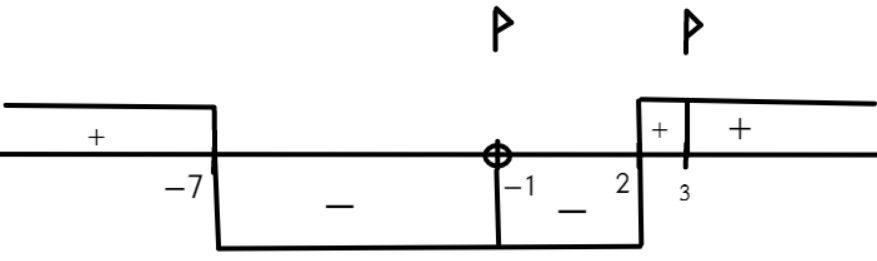
\includegraphics[scale=0.35]{int1.png}}
\end{figure}
$x\in[-7;-1)\cup(-1;2]\cup\{3\}.$\\
2. $\cfrac{(x^2-6x-16)(x+5)^2}{|x-2|}\leqslant0\Leftrightarrow\cfrac{(x-8)(x+2)(x+5)^2}{|x-2|}\leqslant0.$ Применив метод интервалов, найдём ответ:
\begin{figure}[ht!]
\center{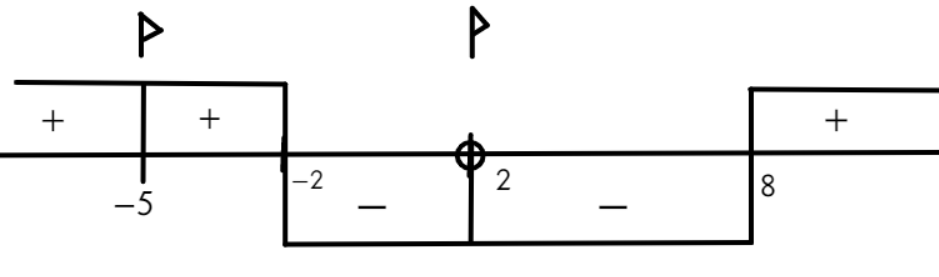
\includegraphics[scale=0.35]{int2.png}}
\end{figure}
$x\in\{-5\}\cup[-2;2)\cup(2;8].$\\
3. $\cfrac{(2x^2+7x-4)(x-3)^2}{x+6}\leqslant0\Leftrightarrow\cfrac{2\left(x-\cfrac{1}{2}\right)(x+4)(x-3)^2}{x+6}\leqslant0.$ Применив метод интервалов, найдём ответ:
\begin{figure}[ht!]
\center{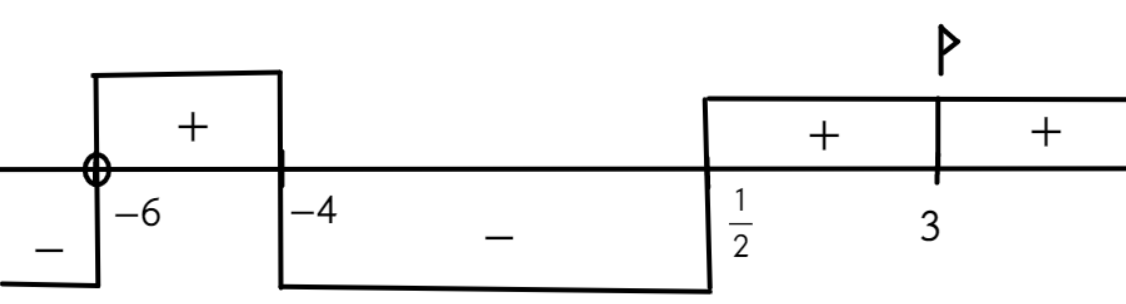
\includegraphics[scale=0.35]{int3.png}}
\end{figure}
$x\in(-\infty; -6)\cup\left[-4;\cfrac{1}{2}\right]\cup\{3\}.$\\
4. $\cfrac{(5x^2+6x+1)(x-2)^2}{x-4}\geqslant0\Leftrightarrow\cfrac{5\left(x+\cfrac{1}{5}\right)(x+1)(x-2)^2}{x-4}\geqslant0.$ Применив метод интервалов, найдём ответ:
\begin{figure}[ht!]
\center{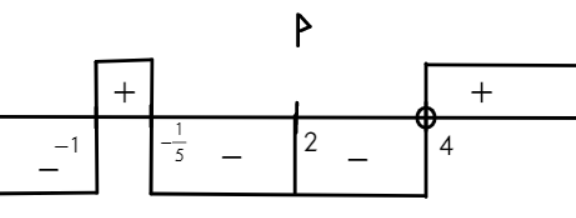
\includegraphics[scale=0.45]{int4.png}}
\end{figure}
$x\in\left[-1;-\cfrac{1}{5}\right]\cup\{2\}\cup(4;+\infty).$\newpage\noindent
5. $\cfrac{(x^2-1)(2x^2-5x-7)}{2-x}\leqslant0\Leftrightarrow\cfrac{(x-1)(x+1)^2\cdot 2\left(x-\cfrac{7}{2}\right)}{2-x}\leqslant0.$ Применив метод интервалов, найдём ответ:
\begin{figure}[ht!]
\center{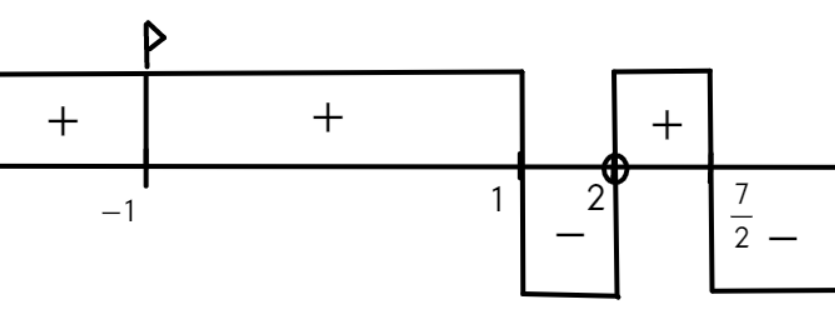
\includegraphics[scale=0.35]{int5.png}}
\end{figure}
$x\in\{-1\}\cup[1;2)\cup\left[\cfrac{7}{2};+\infty\right).$\\
6. $\cfrac{(x^2-1)(2x^2+5x-7)}{3-x}\leqslant0\Leftrightarrow\cfrac{(x-1)^2(x+1)\cdot 2\left(x+\cfrac{7}{2}\right)}{3-x}\leqslant0.$ Применив метод интервалов, найдём ответ:
\begin{figure}[ht!]
\center{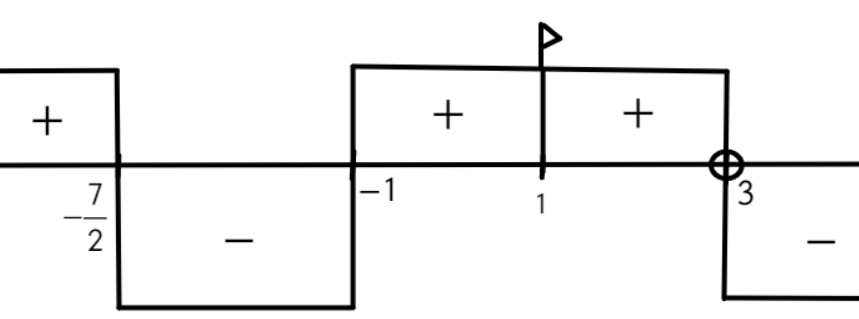
\includegraphics[scale=0.35]{int6.png}}
\end{figure}
$x\in\left[-\cfrac{7}{2};-1\right]\cup\{1\}\cup(3;+\infty).$\\
7. Сделаем замену: $x=\sqrt{a},\ y=\sqrt{b}.$ Тогда исходное неравенство примет вид $x^2+\cfrac{1}{x^2}+y^2+\cfrac{1}{y^2}\geqslant2xy+\cfrac{2}{xy}
\Leftrightarrow x^2-2xy+y^2+\cfrac{1}{x^2}-\cfrac{2}{xy}+\cfrac{1}{y^2}\geqslant0\Leftrightarrow (x-y)^2+\left(\cfrac{1}{x}-\cfrac{1}{y}\right)^2\geqslant0.$ Полученное неравенство верно для любых значений переменных, так как значения квадратов всегда неотрицательны.\\
8. Сделаем замену: $x=\sqrt{a},\ y=\sqrt{b},\ z=\sqrt{c}.$ Тогда исходное неравенство примет вид $x^2+y^2+z^2\geqslant xy+yz+xz\Leftrightarrow
2x^2+2y^2+2z^2\geqslant 2xy+2yz+2xz\Leftrightarrow x^2-2xy+y^2+y^2-2yz+z^2+x^2-2xz+z^2\geqslant 0\Leftrightarrow (x-y)^2+(y-z)^2+(x-z)^2\geqslant 0.$
Полученное неравенство верно для любых значений переменных, так как значения квадратов всегда неотрицательны.\\
9. Сделаем замену: $a=\sqrt{x},\ b=\sqrt{y}.$ Тогда требуется доказать неравенство $a^2-2b^2\leqslant 200$ при том, что $a-b=10.$ Выразим $a$ через $b$ и подставим:
$a=b+10,\ b^2+20b+100-2b^2\leqslant 200,\ b^2-20b+100\geqslant0,\ (b-10)^2\geqslant0.$ Полученное неравенство верно для любых значений переменных, так как значения квадратов всегда неотрицательны.\\
10. Сделаем замену: $a=\sqrt{x},\ b=\sqrt{y}.$ Тогда требуется доказать неравенство $a^2-2b^2\leqslant 128$ при том, что $a-b=8.$ Выразим $a$ через $b$ и подставим:
$a=b+8,\ b^2+16b+64-2b^2\leqslant 128,\ b^2-16b+64\geqslant0,\ (b-8)^2\geqslant0.$ Полученное неравенство верно для любых значений переменных, так как значения квадратов всегда неотрицательны.\\
11. $|2x+5|<x+4\Leftrightarrow\begin{cases}2x+5<x+4,\\ 2x+5>-x-4.\end{cases}
\Leftrightarrow\begin{cases}x<-1,\\ 3x>-9.\end{cases}\Leftrightarrow x\in (-3;-1).$\\
12. $|3x+7|<x+3\Leftrightarrow\begin{cases}3x+7<x+3,\\ 3x+7>-x-3.\end{cases}
\Leftrightarrow\begin{cases}2x<-4,\\ 4x>-10.\end{cases}\Leftrightarrow x\in \left(-\cfrac{5}{2};-2\right).$\newpage\noindent
13. $\sqrt{x}\cdot|1-x|\cdot(2-x)\cdot(3-x^2)\leqslant0 \Leftrightarrow \sqrt{x}\cdot|1-x|\cdot(x-2)\cdot(\sqrt{3}-x)\cdot(\sqrt{3}+x)\geqslant0.$
Применив метод интервалов, найдём ответ:
\begin{figure}[ht!]
\center{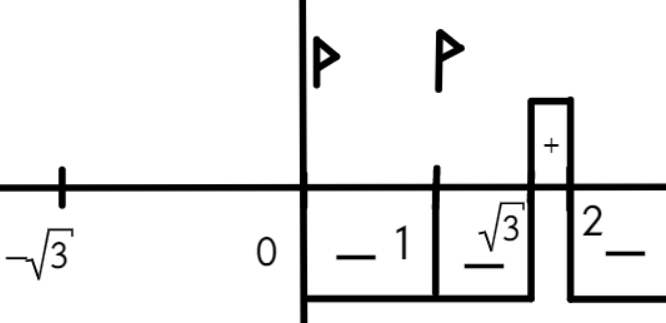
\includegraphics[scale=0.35]{int13.png}}
\end{figure}
$x\in\{0; 1\}\cup[\sqrt{3};2].$\\
14. $\sqrt{x}\cdot(1-x)\cdot|2-x|\cdot(3-x)^2\geqslant0.$
Применив метод интервалов, найдём ответ:
\begin{figure}[ht!]
\center{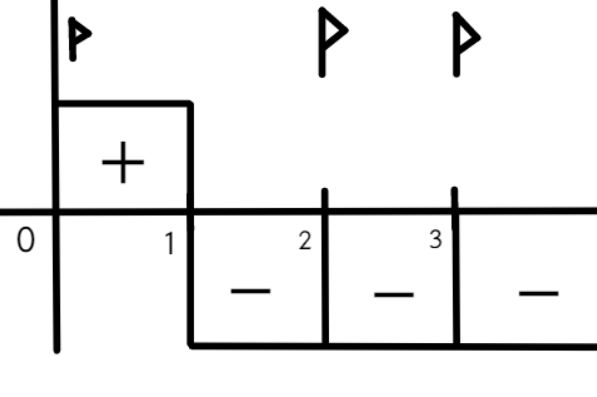
\includegraphics[scale=0.35]{int14.png}}
\end{figure}
$x\in[0;1]\cup\{2; 3\}.$\\
15. $|x+3|-|2x-4|<5\Leftrightarrow |x+3|<|2x-4|+5 \Leftrightarrow \left[\begin{array}{l}\begin{cases} -x-3<-2x+4+5,\\ x\leqslant -3.\end{cases}\\
\begin{cases} x+3<-2x+4+5,\\ -3\leqslant x\leqslant 2 .\end{cases}\\\begin{cases} x+3<2x-4+5,\\ 2\leqslant x.\end{cases}\end{array}\right.\Leftrightarrow
\left[\begin{array}{l}
x\in(-\infty;-3],\\
x\in[-3;2),\\
x\in(2;+\infty).\end{array}\right.\Leftrightarrow x\in(-\infty;2)\cup(2;+\infty)$\\
16. $|x-3|-|2x+4|<5\Leftrightarrow |x-3|<|2x+4|+5 \Leftrightarrow \left[\begin{array}{l}\begin{cases} -x+3<-2x-4+5,\\ x\leqslant -2.\end{cases}\\
\begin{cases} -x+3<2x+4+5,\\ -2\leqslant x\leqslant 3 .\end{cases}\\\begin{cases} -x+3<2x+4+5,\\ 3\leqslant x.\end{cases}\end{array}\right.\Leftrightarrow
\left[\begin{array}{l}
x\in(-\infty;-2),\\
x\in(-2;3],\\
x\in[3;+\infty).\end{array}\right.\Leftrightarrow x\in(-\infty;-2)\cup(-2;+\infty)$\\
17. $\cfrac{x^2+3}{x+1}\leqslant2\Leftrightarrow \cfrac{x^2+3-2x-2}{x+1}\leqslant0\Leftrightarrow \cfrac{(x-1)^2}{x+1}\leqslant0\Leftrightarrow
\left[\begin{array}{l}
x-1=0,\\
x+1<0
\end{array}\right.\Leftrightarrow x \in (-\infty;-1)\cup\{1\}.$\\
18. $\cfrac{x^2}{x-1}\leqslant 4 \Leftrightarrow \cfrac{x^2-4x+4}{x-1}\leqslant 0 \Leftrightarrow \cfrac{(x-2)^2}{x-1}\leqslant 0
\Leftrightarrow
\left[\begin{array}{l}
x-2=0,\\
x-1<0
\end{array}\right.\Leftrightarrow x \in (-\infty;1)\cup\{2\}.$\\
19. $|3x-7|+|x+2|>7\Leftrightarrow \left[\begin{array}{l}\begin{cases} -3x+7-x-2>7,\\ x\leqslant -2.\end{cases}\\
\begin{cases} -3x+7+x+2>7,\\ -2\leqslant x\leqslant \cfrac{7}{3}.\end{cases}\\\begin{cases} 3x-7+x+2>7,\\ \cfrac{7}{3}\leqslant x.\end{cases}\end{array}\right.\Leftrightarrow
\left[\begin{array}{l}
x\in(-\infty;-2],\\
x\in[-2;1),\\
x\in(3;+\infty).\end{array}\right.\Leftrightarrow x\in(-\infty;1)\cup(3;+\infty)$\newpage\noindent
20. $\cfrac{\sqrt{x-3}}{(x-1)(x-5)^2(x-6)}\leqslant0.$
Применив метод интервалов, найдём ответ:
\begin{figure}[ht!]
\center{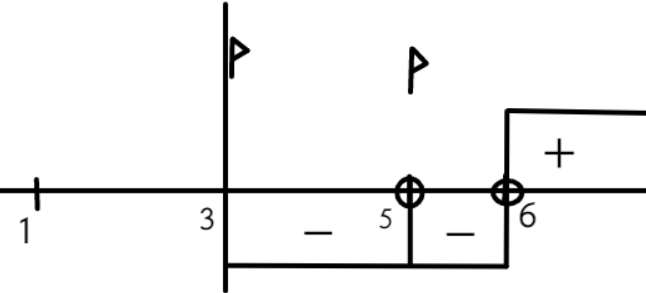
\includegraphics[scale=0.35]{int20.png}}
\end{figure}
$x\in[3;5)\cup(5;6).$\\
21. $\cfrac{\sqrt{x-4}}{(x-2)(x-6)^2(x-7)}\leqslant0.$
Применив метод интервалов, найдём ответ:
\begin{figure}[ht!]
\center{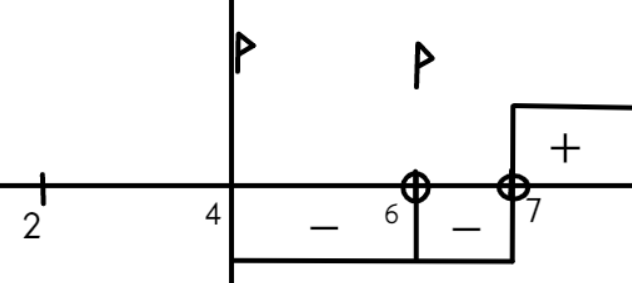
\includegraphics[scale=0.35]{int21.png}}
\end{figure}
$x\in[4;6)\cup(6;7).$\\
22. $|x|\cdot\cfrac{x^3+x^2-x-1}{x^3-x^2-x+1}\geqslant 0\Leftrightarrow|x|\cdot\cfrac{x^2(x+1)-(x+1)}{x^2(x-1)-(x-1)}\geqslant 0\Leftrightarrow
|x|\cdot\cfrac{(x-1)(x+1)^2}{(x-1)^2(x+1)}\geqslant 0.$
Применив метод интервалов, найдём ответ:
\begin{figure}[ht!]
\center{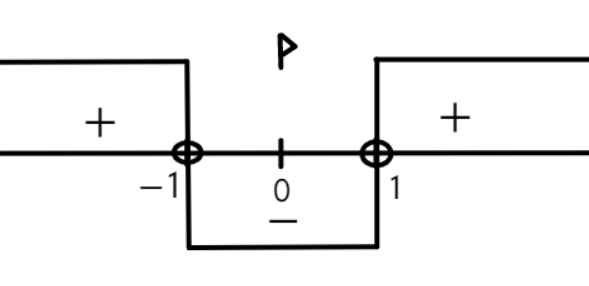
\includegraphics[scale=0.35]{int22.png}}
\end{figure}
$x\in(-\infty;-1)\cup\{0\}\cup(1;+\infty).$\\
23. $|x|\cdot\cfrac{x^3-x^2-x+1}{x^3+x^2-x-1}\geqslant 0\Leftrightarrow|x|\cdot\cfrac{x^2(x-1)-(x-1)}{x^2(x+1)-(x+1)}\geqslant 0\Leftrightarrow
|x|\cdot\cfrac{(x-1)^2(x+1)}{(x-1)(x+1)^2}\geqslant 0.$
Применив метод интервалов, найдём ответ:
\begin{figure}[ht!]
\center{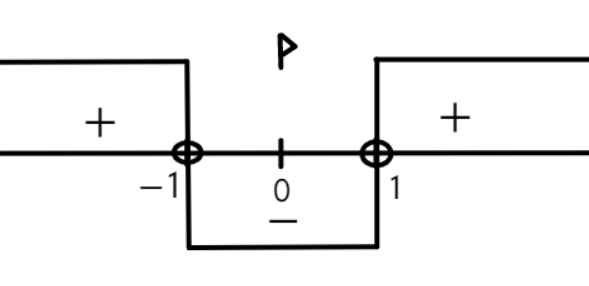
\includegraphics[scale=0.35]{int22.png}}
\end{figure}
$x\in(-\infty;-1)\cup\{0\}\cup(1;+\infty).$\\
24. $|2x-3|<4+x\Leftrightarrow\begin{cases}2x-3<4+x,\\ 2x-3>-4-x.\end{cases}
\Leftrightarrow\begin{cases}x<7,\\ 3x>-1.\end{cases}\Leftrightarrow
x\in\left(-\cfrac{1}{3};7\right).$\\
25. $|2x-1|<5+x\Leftrightarrow\begin{cases}2x-1<5+x,\\ 2x-1>-5-x.\end{cases}
\Leftrightarrow\begin{cases}x<6,\\ 3x>-4.\end{cases}\Leftrightarrow x\in \left(-\cfrac{4}{3};6\right).$\\
26. $\cfrac{(x-1)^2(x+3)(x-3)}{\sqrt{x+2}}\geqslant0.$ Применив метод интервалов, найдём ответ:
\begin{figure}[ht!]
\center{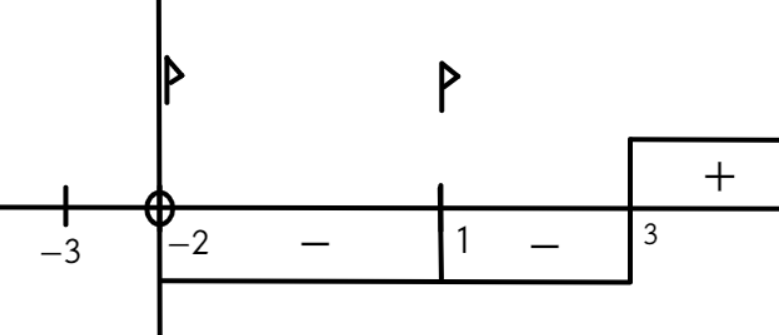
\includegraphics[scale=0.35]{int26.png}}
\end{figure}
$x\in\{1\}\cup[3;+\infty).$\newpage\noindent
27. $\cfrac{(x-2)^2(x+2)(x-4)}{\sqrt{x+1}}\geqslant0.$
Применив метод интервалов, найдём ответ:
\begin{figure}[ht!]
\center{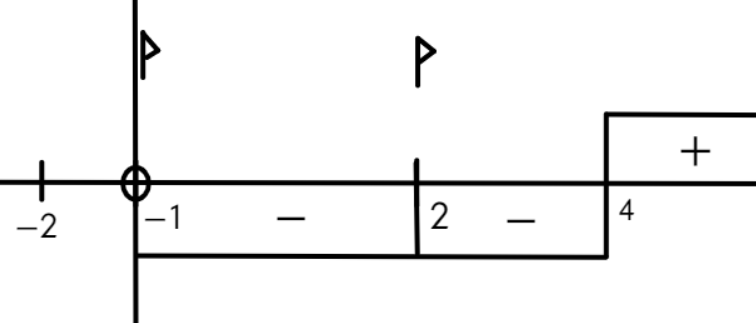
\includegraphics[scale=0.35]{int27.png}}
\end{figure}
$x\in\{2\}\cup[4;+\infty).$\\
28. $\cfrac{x^2-3}{x+2}\geqslant-6\Leftrightarrow \cfrac{x^2-3+6x+12}{x+2}\geqslant0\Leftrightarrow \cfrac{(x+3)^2}{x+2}\geqslant0
\Leftrightarrow
\left[\begin{array}{l}
x+3=0,\\
x+2>0
\end{array}\right.\Leftrightarrow x \in \{-3\}\cup(-2;+\infty).$\\
29. $\cfrac{x^2-3}{x-2}\leqslant 6\Leftrightarrow \cfrac{x^2-3-6x+12}{x-2}\leqslant0\Leftrightarrow \cfrac{(x-3)^2}{x-2}\leqslant0
\Leftrightarrow
\left[\begin{array}{l}
x-3=0,\\
x-2<0
\end{array}\right.\Leftrightarrow x \in (-\infty;2)\cup\{3\}.$\\
30. $\cfrac{(x-1)^2(x^2-x-2)}{x^2+3x+2}\geqslant0\Leftrightarrow\cfrac{(x-1)^2(x-2)(x+1)}{(x+2)(x+1)}\geqslant0.$
Применив метод интервалов, найдём ответ:
\begin{figure}[ht!]
\center{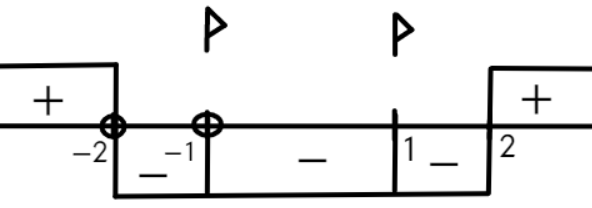
\includegraphics[scale=0.35]{int30.png}}
\end{figure}
$x\in(-\infty;-2)\cup\{1\}\cup[2;+\infty).$\\
31. $\cfrac{(x+1)^2(x^2+x-2)}{x^2-3x+2}\geqslant0\Leftrightarrow\cfrac{(x+1)^2(x+2)(x-1)}{(x-2)(x-1)}\geqslant0.$
Применив метод интервалов, найдём ответ:
\begin{figure}[ht!]
\center{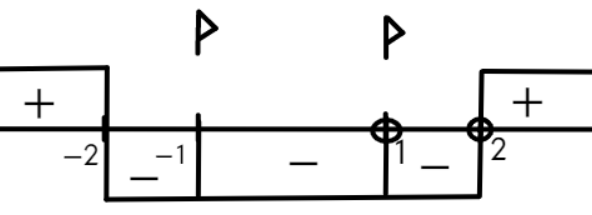
\includegraphics[scale=0.35]{int31.png}}
\end{figure}
$x\in(-\infty;-2]\cup\{-1\}\cup(2;+\infty).$\\
32. $\cfrac{x^2}{x+2}\leqslant -x\Leftrightarrow\cfrac{x^2+x^2+2x}{x+2}\leqslant 0\Leftrightarrow\cfrac{2x(x+1)}{x+2}\leqslant 0.$
Применив метод интервалов, найдём ответ:
\begin{figure}[ht!]
\center{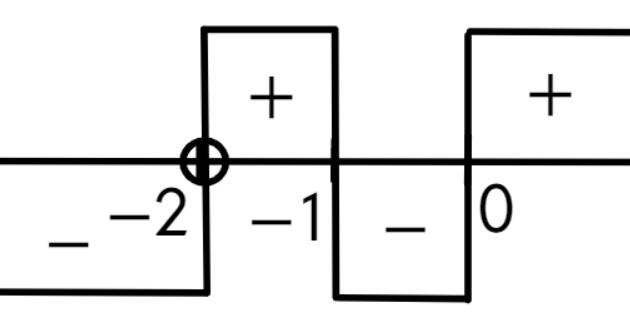
\includegraphics[scale=0.35]{int32.png}}
\end{figure}
$x\in(-\infty;-2)\cup[-1;0].$\\
33. $\cfrac{x^2}{2-x}\leqslant x \Leftrightarrow\cfrac{x^2-2x+x^2}{2-x}\leqslant 0\Leftrightarrow\cfrac{2x(x-1)}{2-x}\leqslant 0.$
Применив метод интервалов, найдём ответ:
\begin{figure}[ht!]
\center{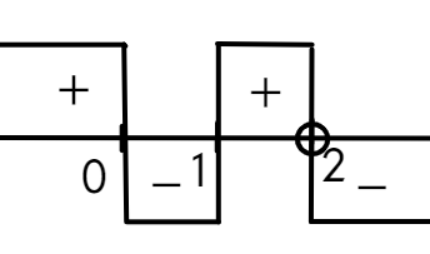
\includegraphics[scale=0.35]{int33.png}}
\end{figure}
$x\in[0;1]\cup(2;+\infty).$\\
34. $|3x+2|\geqslant x^2-2\Leftrightarrow\left[\begin{array}{l}3x+2\geqslant x^2-2,\\ 3x+2\leqslant -x^2+2.\end{array}\right.\Leftrightarrow
\left[\begin{array}{l}x^2-3x-4\leqslant 0,\\ x^2+3x\leqslant 0.\end{array}\right.\Leftrightarrow
\left[\begin{array}{l}(x-4)(x+1)\leqslant 0,\\ x(x+3)\leqslant 0.\end{array}\right.
\Leftrightarrow
\left[\begin{array}{l}x\in[-1;4],\\ x\in[-3;0].\end{array}\right.\Leftrightarrow
x\in[-3;4].$\\
35. $|2-3x|\geqslant x^2-2\Leftrightarrow\left[\begin{array}{l}2-3x\geqslant x^2-2,\\ 2-3x\leqslant -x^2+2.\end{array}\right.\Leftrightarrow
\left[\begin{array}{l}x^2+3x-4\leqslant 0,\\ x^2-3x\leqslant 0.\end{array}\right.\Leftrightarrow
\left[\begin{array}{l}(x+4)(x-1)\leqslant 0,\\ x(x-3)\leqslant 0.\end{array}\right.
\Leftrightarrow
\left[\begin{array}{l}x\in[-4;1],\\ x\in[0;3].\end{array}\right.\Leftrightarrow
x\in[-4;3].$\\
36. $\cfrac{3}{x}<5\Leftrightarrow \cfrac{5\left(\cfrac{3}{5}-x\right)}{x}<0\Leftrightarrow x\in(-\infty;0)\cup\left(\cfrac{3}{5};+\infty\right).$\\
37. $\cfrac{7}{x}<4\Leftrightarrow \cfrac{4\left(\cfrac{7}{4}-x\right)}{x}<0\Leftrightarrow x\in(-\infty;0)\cup\left(\cfrac{7}{4};+\infty\right).$\\
38. $x^2-3x+2>|x-5|\Leftrightarrow \begin{cases}x-5<x^2-3x+2,\\ x-5>-x^2+3x-2.\end{cases}
\Leftrightarrow \begin{cases}x^2-4x+7>0,\\ x^2-2x-3>0.\end{cases}
\Leftrightarrow \begin{cases}(x-2)^2+3>0,\\ (x-3)(x+1)>0.\end{cases}$\\$\Leftrightarrow x\in (-\infty;-1)\cup(3;+\infty).$\\
39. $x^2-5x+6>|x-6|\Leftrightarrow \begin{cases}x-6<x^2-5x+6,\\ x-6>-x^2+5x-6.\end{cases}
\Leftrightarrow \begin{cases}x^2-6x+12>0,\\ x^2-4x>0.\end{cases}
\Leftrightarrow \begin{cases}(x-3)^2+3>0,\\ x(x-4)>0.\end{cases}$\\$\Leftrightarrow x\in (-\infty;0)\cup(4;+\infty).$\\
40. $\cfrac{1}{x-2}+\cfrac{1}{x-1}\geqslant\cfrac{1}{x}\Leftrightarrow \cfrac{x(x-1)+x(x-2)-(x-1)(x-2)}{x(x-1)(x-2)}\geqslant0\Leftrightarrow$\\$
\cfrac{x^2-x+x^2-2x-x^2+2x+x-2}{x(x-1)(x-2)}\geqslant0\Leftrightarrow\cfrac{(x-\sqrt{2})(x+\sqrt{2})}{x(x-1)(x-2)}\geqslant0.$\\ Применив метод интервалов, найдём ответ:
\begin{figure}[ht!]
\center{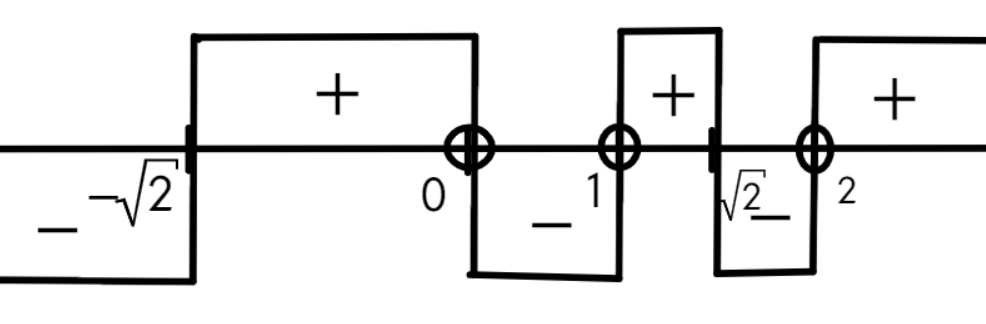
\includegraphics[scale=0.35]{int40.png}}
\end{figure}
$x\in[-\sqrt{2};0)\cup(1;\sqrt{2}]\cup(2;+\infty).$\\
41. $\cfrac{1}{x+2}+\cfrac{1}{x+1}\geqslant\cfrac{1}{x}\Leftrightarrow \cfrac{x(x+1)+x(x+2)-(x+1)(x+2)}{x(x+1)(x+2)}\geqslant0\Leftrightarrow$\\$
\cfrac{x^2+x+x^2+2x-x^2-2x-x-2}{x(x+1)(x+2)}\geqslant0\Leftrightarrow\cfrac{(x-\sqrt{2})(x+\sqrt{2})}{x(x+1)(x+2)}\geqslant0.$\\ Применив метод интервалов, найдём ответ:
\begin{figure}[ht!]
\center{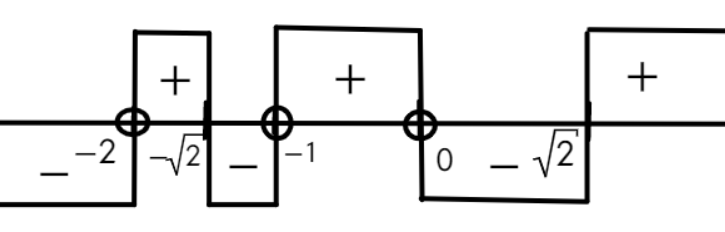
\includegraphics[scale=0.35]{int41.png}}
\end{figure}
$x\in(-2;-\sqrt{2}]\cup(-1;0)\cup[\sqrt{2};+\infty).$\newpage\noindent
42. $\cfrac{1}{x-2}+\cfrac{1}{x-3}\geqslant\cfrac{1}{x}\Leftrightarrow \cfrac{x(x-3)+x(x-2)-(x-3)(x-2)}{x(x-2)(x-3)}\geqslant0\Leftrightarrow$\\$
\cfrac{x^2-3x+x^2-2x-x^2+2x+3x-6}{x(x-2)(x-3)}\geqslant0\Leftrightarrow\cfrac{(x-\sqrt{6})(x+\sqrt{6})}{x(x-2)(x-3)}\geqslant0.$\\ Применив метод интервалов, найдём ответ:
\begin{figure}[ht!]
\center{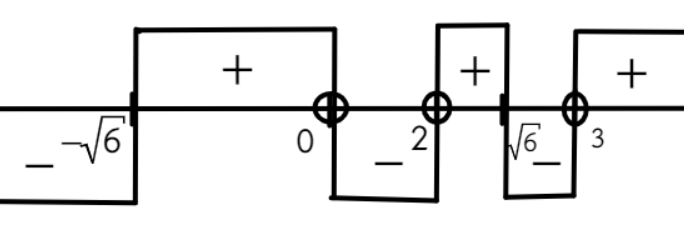
\includegraphics[scale=0.35]{int42.png}}
\end{figure}
$x\in[-\sqrt{6};0)\cup(2;\sqrt{6}]\cup(3;+\infty).$\\
43. $\cfrac{1}{x+2}+\cfrac{1}{x+3}\geqslant\cfrac{1}{x}\Leftrightarrow \cfrac{x(x+3)+x(x+2)-(x+3)(x+2)}{x(x+2)(x+3)}\geqslant0\Leftrightarrow$\\$
\cfrac{x^2+3x+x^2+2x-x^2-2x-3x-6}{x(x+2)(x+3)}\geqslant0\Leftrightarrow\cfrac{(x-\sqrt{6})(x+\sqrt{6})}{x(x+2)(x+3)}\geqslant0.$\\ Применив метод интервалов, найдём ответ:
\begin{figure}[ht!]
\center{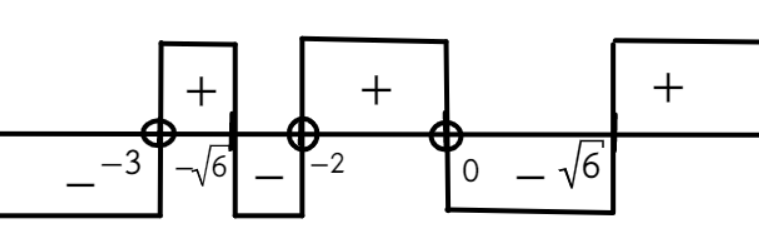
\includegraphics[scale=0.35]{int43.png}}
\end{figure}
$x\in(-3;-\sqrt{6}]\cup(-2;0)\cup[\sqrt{6};+\infty).$\\
44. $|x^2-6x-7|\geqslant-6x+7\Leftrightarrow \left[\begin{array}{l}x^2-6x-7\geqslant -6x+7,\\ x^2-6x-7\leqslant 6x-7.\end{array}\right.
\Leftrightarrow \left[\begin{array}{l}(x-\sqrt{14})(x+\sqrt{14})\geqslant 0,\\ x(x-12)\leqslant 0.\end{array}\right.
\Leftrightarrow$\\$ \left[\begin{array}{l}x\in(-\infty;-\sqrt{14}]\cup[\sqrt{14};+\infty),\\ x\in[0;12].\end{array}\right.\Leftrightarrow
x\in(-\infty;-\sqrt{14}]\cup[0;+\infty).$\\
45. $|x^2-2x-15|\leqslant-2x+15\Leftrightarrow \begin{cases}x^2-2x-15\leqslant -2x+15,\\ x^2-2x-15\geqslant 2x-15.\end{cases}
\Leftrightarrow \begin{cases}(x-\sqrt{30})(x+\sqrt{30})\leqslant 0,\\ x(x-4)\geqslant 0.\end{cases}
\Leftrightarrow$\\$ \begin{cases} x\in[-\sqrt{30};\sqrt{30}],\\ x\in(-\infty;0]\cup[4;+\infty).\end{cases}\Leftrightarrow
x\in[-\sqrt{30};0]\cup[4;\sqrt{30}].$\\
46. $\cfrac{x^2-2x-8}{x-4}\leqslant 7\Leftrightarrow \cfrac{x^2-2x-8-7x+28}{x-4}\leqslant0 \Leftrightarrow \cfrac{(x-5)(x-4)}{x-4}\leqslant0
\Leftrightarrow \begin{cases}x-5\leqslant 0,\\ x-4\neq0.\end{cases}\Leftrightarrow$\\$ x\in (-\infty;4)\cup(4;5].$\\
47. $\cfrac{x^2-4x-5}{x-5}\leqslant 7\Leftrightarrow \cfrac{x^2-4x-5-7x+35}{x-5}\leqslant0 \Leftrightarrow \cfrac{(x-5)(x-6)}{x-5}\leqslant0
\Leftrightarrow \begin{cases}x-6\leqslant 0,\\ x-5\neq0.\end{cases}\Leftrightarrow$\\$ x\in (-\infty;5)\cup(5;6].$\\
48. $\cfrac{7}{(x-1)(x-2)}+\cfrac{9}{x-2}+1\leqslant0\Leftrightarrow \cfrac{7+9x-9+x^2-2x-x+2}{(x-1)(x-2)}\leqslant0
\Leftrightarrow \cfrac{x(x+6)}{(x-1)(x-2)}\leqslant0.$ Применив метод интервалов, найдём ответ:
\begin{figure}[ht!]
\center{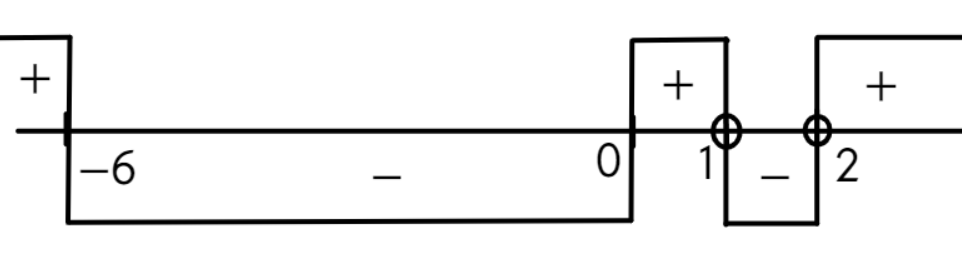
\includegraphics[scale=0.35]{int48.png}}
\end{figure}
$x\in[-6;0]\cup(1;2).$\newpage\noindent
49. $\cfrac{1}{3-x}\geqslant\cfrac{1}{(x^2-9)(3-x)}\Leftrightarrow\cfrac{-1}{(x-3)^2(x+3)}-\cfrac{1}{3-x}\leqslant0\Leftrightarrow
\cfrac{-1+x^2-9}{(x-3)^2(x+3)}\leqslant0\Leftrightarrow$\\$\cfrac{(x-\sqrt{10})(x+\sqrt{10})}{(x-3)^2(x+3)}\leqslant0.$\\ Применив метод интервалов, найдём ответ:
\begin{figure}[ht!]
\center{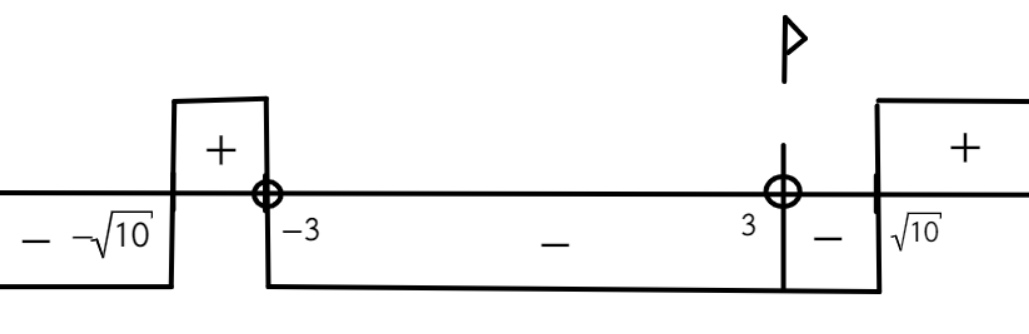
\includegraphics[scale=0.35]{int49.png}}
\end{figure}
$x\in(-\infty;-\sqrt{10}]\cup(-3;3)\cup(3;\sqrt{10}].$\\
50. $\cfrac{1}{(4-x^2)(x-2)}\leqslant\cfrac{1}{2-x} \Leftrightarrow\cfrac{-1}{(x-2)^2(x+2)}-\cfrac{1}{2-x}\leqslant0\Leftrightarrow
\cfrac{-1+x^2-4}{(x-2)^2(x+2)}\leqslant0\Leftrightarrow$\\$\cfrac{(x-\sqrt{5})(x+\sqrt{5})}{(x-2)^2(x+2)}\leqslant0.$\\ Применив метод интервалов, найдём ответ:
\begin{figure}[ht!]
\center{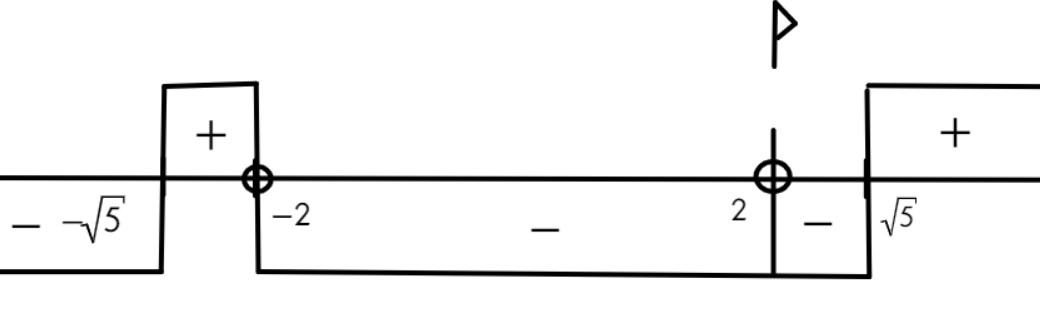
\includegraphics[scale=0.35]{int50.png}}
\end{figure}
$x\in(-\infty;-\sqrt{5}]\cup(-2;2)\cup(2;\sqrt{5}].$\\
51. $\cfrac{x^2-(\sqrt{3}+\sqrt{7})x+\sqrt{21}}{\sqrt{5-x}}\cdot\cfrac{x^2-4x+4}{6x-x^2-9}\leqslant 0\Leftrightarrow
\cfrac{(x-\sqrt{3})(x-\sqrt{7})(x-2)^2}{\sqrt{5-x}(x-3)^2}\geqslant 0.$ Применив метод интервалов, найдём ответ:
\begin{figure}[ht!]
\center{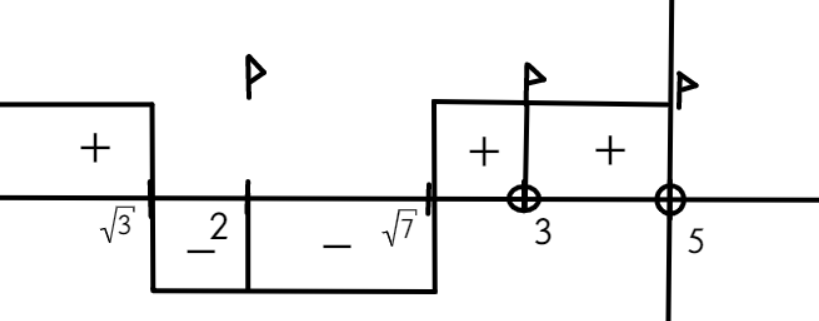
\includegraphics[scale=0.35]{int51.png}}
\end{figure}
$x\in(-\infty;\sqrt{3}]\cup\{2\}\cup[\sqrt{7};3)\cup(3;5).$\\
52. $\cfrac{\sqrt{x}}{2x-1}\geqslant\cfrac{\sqrt{x}}{x-5}\Leftrightarrow\sqrt{x}\cdot\left(\cfrac{1}{2x-1}-\cfrac{1}{x-5}\right)\geqslant0\Leftrightarrow
\cfrac{\sqrt{x}(-4-x)}{(2x-1)(x-5)}\geqslant0.$ Применив метод интервалов, найдём ответ:
\begin{figure}[ht!]
\center{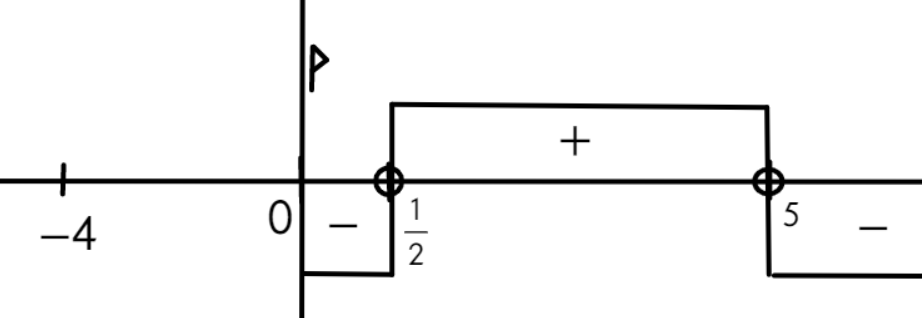
\includegraphics[scale=0.35]{int52.png}}
\end{figure}
$x\in\{0\}\cup\left(\cfrac{1}{2};5\right).$\\
53. $x\sqrt{x+2}>x\Leftrightarrow x(\sqrt{x+2}-1)>0.$ Это неравенство также можно решить методом интервалов, поставив на числовом луче две точки 0 и $-1$ (так как второй множитель равен нулю при  $x=-1).$ По ОДЗ значение $x$ не может быть меньше $-2,$ поэтому получим ответ $x\in[-2;-1)\cup(0;+\infty).$\newpage\noindent
54. $\cfrac{3x^2+2x^3-x^4}{\sqrt{x+2}}\leqslant0\Leftrightarrow\cfrac{x^2(3+2x-x^2)}{\sqrt{x+2}}\leqslant0
\Leftrightarrow\cfrac{x^2(x-3)(x+1)}{\sqrt{x+2}}\geqslant0.$ Применив метод интервалов, найдём ответ:
\begin{figure}[ht!]
\center{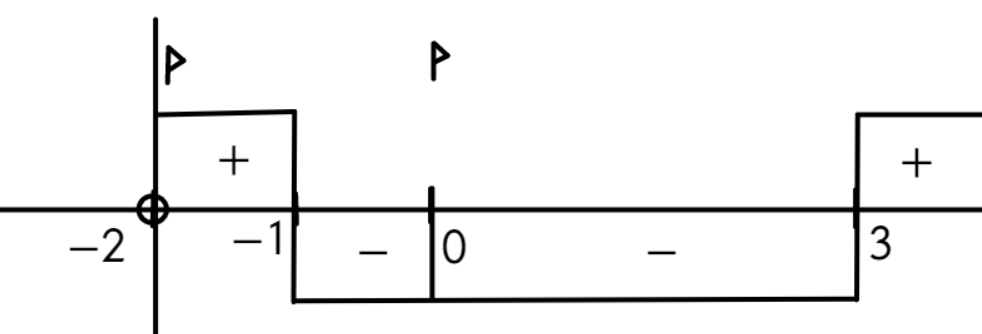
\includegraphics[scale=0.35]{int54.png}}
\end{figure}
$x\in(-2;-1]\cup\{0\}\cup[3;+\infty).$\\
55. $x|x-2|\leqslant x-2\Leftrightarrow \left[\begin{array}{l}x-2=0,\\ x \leqslant \cfrac{x-2}{|x-2|}.\end{array}\right.
\Leftrightarrow \left[\begin{array}{l}x=2,\\ \begin{cases}x \leqslant 1,\\ x>2.\end{cases}\\ \begin{cases}x \leqslant -1,\\ x<2.\end{cases} \end{array}\right.
\Leftrightarrow x\in (-\infty;-1]\cup\{2\}.$\\
56. $-\cfrac{1}{2}x^2+2,5x-3\geqslant0\Leftrightarrow x^2-5x+6\leqslant0\Leftrightarrow (x-2)(x-3)\leqslant0\Leftrightarrow
x\in[2;3].$\\
57. $\cfrac{4}{x^2-x-6}\geqslant\cfrac{1}{2+x}\Leftrightarrow\cfrac{4}{(x-3)(x+2)}-\cfrac{1}{x+2}\geqslant0\Leftrightarrow
\cfrac{7-x}{(x-3)(x+2)}\geqslant0.$ Применив метод интервалов, найдём ответ:
\begin{figure}[ht!]
\center{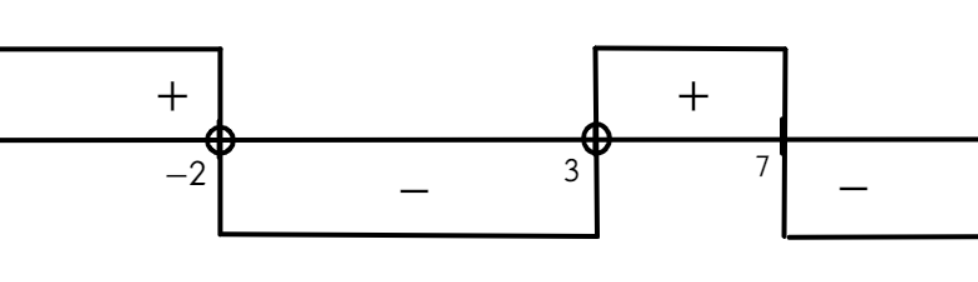
\includegraphics[scale=0.35]{int57.png}}
\end{figure}
$x\in(-\infty;-2)\cup(3;7].$\\
58. $x^2-x>|x+3|\Leftrightarrow \begin{cases}x+3<x^2-x,\\ x+3>-x^2+x.\end{cases}\Leftrightarrow \begin{cases}x^2-2x-3>0,\\ x^2+3>0.\end{cases}\Leftrightarrow
(x-3)(x+1)>0\Leftrightarrow $\\$x\in(-\infty;-1)\cup(3;+\infty).$\\
59. $|x^2-3|<|3-x|\Leftrightarrow (x^2-3+3-x)(x^2-3-3+x)<0 \Leftrightarrow x(x-1)(x+3)(x-2)<0.$ Применив метод интервалов, найдём ответ:
\begin{figure}[ht!]
\center{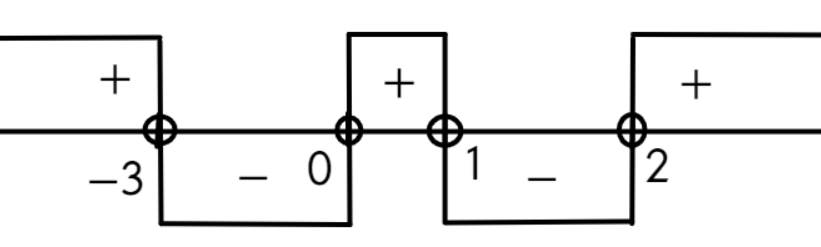
\includegraphics[scale=0.35]{int59.png}}
\end{figure}
$x\in(-3;0)\cup(1;2).$\\
60. $\cfrac{x^2-20}{5x^2+12}\leqslant\cfrac{x-8}{5x^2+12}\Leftrightarrow\cfrac{x^2-20-x+8}{5x^2+12}\leqslant0\Leftrightarrow
\cfrac{(x-4)(x+3)}{5x^2+12}\leqslant0\Leftrightarrow x\in [-3;4].$\\
61. $\left(1+\left(x-\cfrac{3}{2}\right):3\right)\left(-0,75\right)<0\Leftrightarrow1+\left(x-\cfrac{3}{2}\right):3>0\Leftrightarrow
x-\cfrac{3}{2}>-3\Leftrightarrow x\in  \left(-\cfrac{3}{2};+\infty\right).$\\
62. $x^2+x>|x-3|\Leftrightarrow \begin{cases}x-3<x^2+x,\\ x-3>-x^2-x.\end{cases}\Leftrightarrow \begin{cases}x^2+3>0,\\ x^2+2x-3>0.\end{cases}\Leftrightarrow
(x+3)(x-1)>0\Leftrightarrow $\\$x\in(-\infty;-3)\cup(1;+\infty).$\\
63. Если $x<6,$ то по крайней мере первое из чисел меньше 6, а значит меньшее из двух чисел точно меньше 6. Если же $x\geqslant6,$ то и $x^2-3\geqslant36-3=33>6.$ Таким образом, подходят только значения $x<6.$\\
64. Чтобы минимальное из двух чисел было не меньше 4, необходимо и достаточно, чтобы они оба были не меньше 4. То есть, надо решить систему неравенств\\
$\begin{cases}x+15 \geqslant 4,\\ x^2+3\geqslant 4.\end{cases}\Leftrightarrow
\begin{cases}x \geqslant -11,\\(x-1)(x+1)\geqslant 0.\end{cases}\Leftrightarrow
\begin{cases}x \geqslant -11,\\ x\in(-\infty;-1]\cup[1;+\infty).\end{cases}\Leftrightarrow
x \in [-11;-1]\cup[1;+\infty).$\\
65. Чтобы максимальное из двух чисел было не меньше 1, необходимо и достаточно, чтобы хотя бы одно из них было не меньше 1. То есть, надо решить совокупность неравенств\\ $\left[\begin{array}{l}x\geqslant 1,\\ x^2-3 \geqslant1 .  \end{array}\right.\Leftrightarrow
\left[\begin{array}{l}x\geqslant 1,\\ (x-2)(x+2) \geqslant 0 .  \end{array}\right.\Leftrightarrow
\left[\begin{array}{l}x\geqslant 1,\\ x\in (-\infty;-2]\cup[2;+\infty).  \end{array}\right.\Leftrightarrow
x\in (-\infty;-2]\cup[1;+\infty).$\\
66. $\cfrac{2x^3+3x^2}{x-2}\geqslant0\Leftrightarrow\cfrac{2x^2\left(x+\cfrac{3}{2}\right)}{x-2}\geqslant0.$\\ Применив метод интервалов, найдём ответ:
\begin{figure}[ht!]
\center{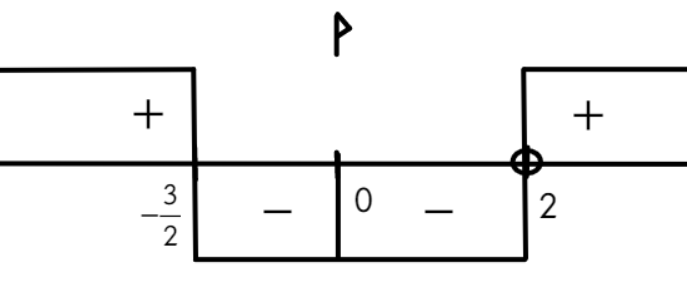
\includegraphics[scale=0.35]{int66.png}}
\end{figure}
$x\in\left(-\infty;-\cfrac{3}{2}\right]\cup\{0\}\cup(2;+\infty).$\\
67. $\cfrac{2x^3-3x^2}{x+2}\geqslant0\Leftrightarrow\cfrac{2x^2\left(x-\cfrac{3}{2}\right)}{x+2}\geqslant0.$\\ Применив метод интервалов, найдём ответ:
\begin{figure}[ht!]
\center{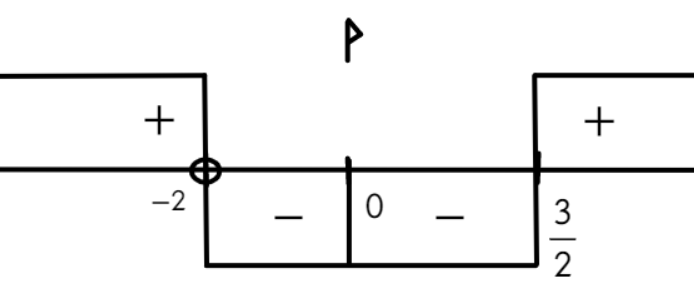
\includegraphics[scale=0.35]{int67.png}}
\end{figure}
$x\in\left(-\infty;-2\right)\cup\{0\}\cup\left[\cfrac{3}{2};+\infty\right).$\\
68. $\cfrac{|3x+2|}{x}<-1\Leftrightarrow\cfrac{|3x+2|+x}{x}<0\Leftrightarrow
\left[\begin{array}{l}\begin{cases}\cfrac{-2(x+1)}{x}<0,\\ x\leqslant-\cfrac{2}{3}.\end{cases}\\ \begin{cases}\cfrac{4\left(x+\cfrac{1}{2}\right)}{x}<0,\\ x\geqslant-\cfrac{2}{3}.\end{cases}  \end{array}\right.\Leftrightarrow\left[\begin{array}{l} x\in\left(-\infty;-1\right),\\
x\in\left(-\cfrac{1}{2};0\right)\end{array}\right.\Leftrightarrow$\\$ x\in\left(-\infty;-1\right)\cup\left(-\cfrac{1}{2};0\right).$\\
69. $\cfrac{|2x+1|}{x}<-1\Leftrightarrow\cfrac{|2x+1|+x}{x}<0\Leftrightarrow
\left[\begin{array}{l}\begin{cases}\cfrac{-x-1}{x}<0,\\ x\leqslant-\cfrac{1}{2}.\end{cases}\\ \begin{cases}\cfrac{3\left(x+\cfrac{1}{3}\right)}{x}<0,\\ x\geqslant-\cfrac{1}{2}.\end{cases}  \end{array}\right.\Leftrightarrow\left[\begin{array}{l} x\in\left(-\infty;-1\right),\\
x\in\left(-\cfrac{1}{3};0\right)\end{array}\right.\Leftrightarrow$\\$ x\in\left(-\infty;-1\right)\cup\left(-\cfrac{1}{3};0\right).$\\
70. $|2x+5|+x<7\Leftrightarrow |2x+5|<7-x\Leftrightarrow \begin{cases}2x+5<7-x,\\ 2x+5>-7+x.\end{cases}
\Leftrightarrow \begin{cases}x<\cfrac{2}{3},\\ x>-12.\end{cases}\Leftrightarrow x\in\left(-12;\cfrac{2}{3}\right).$\\
71. $\cfrac{x^3+2x^2+7}{7-x}\geqslant1\Leftrightarrow\cfrac{x^3+2x^2+7-7+x}{7-x}\geqslant0\Leftrightarrow
\cfrac{x(x+1)^2}{7-x}\geqslant0.$ Применив метод интервалов, найдём ответ:
\begin{figure}[ht!]
\center{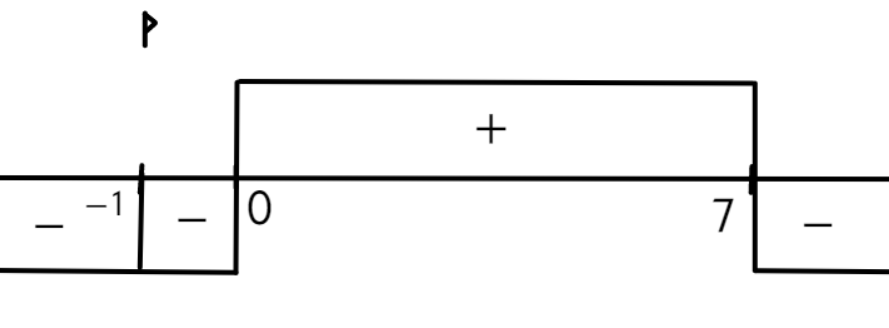
\includegraphics[scale=0.35]{int71.png}}
\end{figure}
$x\in\{-1\}\cup[0;7).$\\
72. $\cfrac{(x+1)(x-8)^4}{(x+2)^2(5-x)}\geqslant0.$ Применив метод интервалов, найдём ответ:
\begin{figure}[ht!]
\center{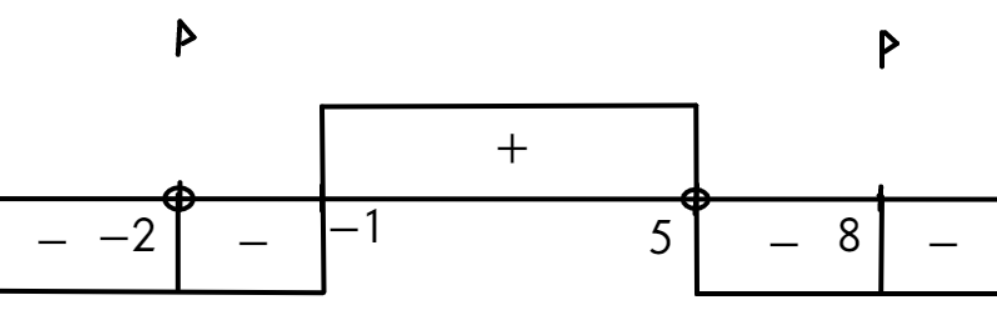
\includegraphics[scale=0.35]{int72.png}}
\end{figure}
$x\in[-1;5)\cup\{8\}.$\\
73. $\cfrac{x^2(x^2-2x+1)}{(x+7)^3(3-x)}\leqslant0\Leftrightarrow\cfrac{x^2(x-1)^2}{(x+7)^3(3-x)}\leqslant0.$\\ Применив метод интервалов, найдём ответ:
\begin{figure}[ht!]
\center{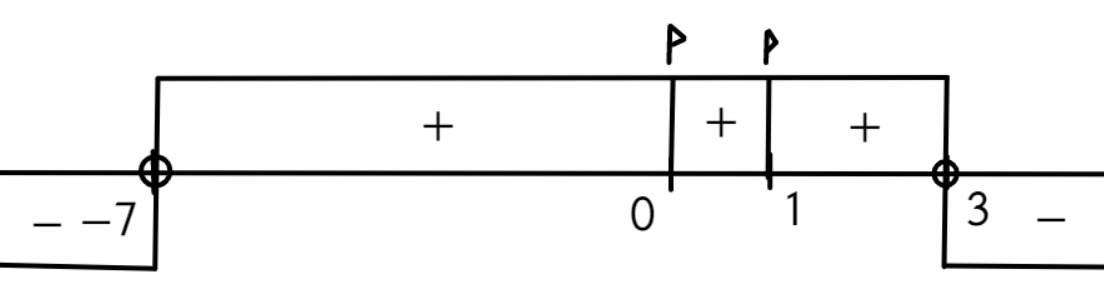
\includegraphics[scale=0.35]{int73.png}}
\end{figure}
$x\in(-\infty;-7)\cup\{0;1\}\cup(3;+\infty).$\\
74. $(2-\sqrt{5})x>2+\sqrt{5}\Leftrightarrow x<\cfrac{2+\sqrt{5}}{2-\sqrt{5}}=\cfrac{4+4\sqrt{5}+5}{4-5}=-9-4\sqrt{5}=-9-\sqrt{80}.$ Так как $9+\sqrt{80}<9+9=18,$
наибольшим целым решением неравенства является $x=-18.$\\
75. $(\sqrt{3}-2)x>\sqrt{3}+2\Leftrightarrow x<\cfrac{\sqrt{3}+2}{\sqrt{3}-2}=\cfrac{3+4\sqrt{3}+4}{3-4}=-7-4\sqrt{3}=-7-\sqrt{48}.$ Так как $7+\sqrt{48}<7+7=14,$
наибольшим целым решением неравенства является $x=-14.$\\
76. $|x-3|<6-3x\Leftrightarrow\begin{cases} x-3<6-3x,\\x-3>-6+3x.\end{cases}
\Leftrightarrow\begin{cases} x<\cfrac{9}{4},\\ x<\cfrac{3}{2}.\end{cases}\Leftrightarrow x\in\left(-\infty;\cfrac{3}{2}\right)$\\
77. $|x-4|>2x-1\Leftrightarrow\left[\begin{array}{l}x-4>2x-1,\\x-4<-2x+1.\end{array}\right.
\Leftrightarrow\left[\begin{array}{l}x<-3,\\x<\cfrac{5}{3}.\end{array}\right.\Leftrightarrow x\in\left(-\infty;\cfrac{5}{3}\right).$\\
78. $|2x-7|<x \Leftrightarrow \begin{cases} 2x-7<x,\\ 2x-7> -x\end{cases} \Leftrightarrow \begin{cases} x<7,\\ x>\cfrac{7}{3}\end{cases}
\Leftrightarrow x\in\left(\cfrac{7}{3};7\right).$\\
79. $|2x-5|<x \Leftrightarrow \begin{cases} 2x-5<x,\\ 2x-5> -x\end{cases} \Leftrightarrow \begin{cases} x<5,\\ x>\cfrac{5}{3}\end{cases}
\Leftrightarrow x\in\left(\cfrac{5}{3};5\right).$\\
80. $\cfrac{\sqrt{x+3}(2x^2+13x+15)(x^2+4x-5)(2x+3)}{x^2-1}\geqslant0 \Leftrightarrow \cfrac{\sqrt{x+3}\cdot4\left(x+\cfrac{3}{2}\right)^2(x+5)^2(x-1)}{(x-1)(x+1)}\geqslant0.$ Применив метод интервалов, найдём ответ:
\begin{figure}[ht!]
\center{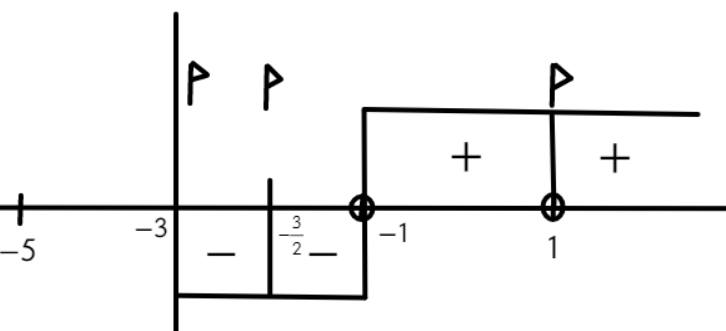
\includegraphics[scale=0.35]{int80.png}}
\end{figure}
$x\in\left\{-3;-\cfrac{3}{2}\right\}\cup(-1;1)\cup(1;+\infty).$\\
81. $\cfrac{\sqrt{x+4}(2x^2+13x+20)(x^2+4x-12)(2x+5)}{x^2-4}\geqslant0\Leftrightarrow \cfrac{\sqrt{x+4}\cdot4\left(x+\cfrac{5}{2}\right)^2(x+4)(x+6)(x-2)}{(x-2)(x+2)}\geqslant0.$ Применив метод интервалов, найдём ответ:
\begin{figure}[ht!]
\center{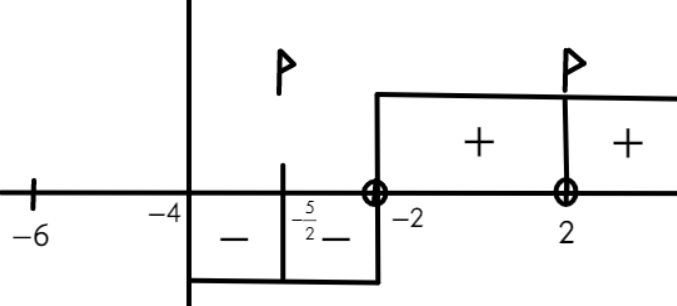
\includegraphics[scale=0.35]{int81.png}}
\end{figure}
$x\in\left\{-4;-\cfrac{5}{2}\right\}\cup(-2;2)\cup(2;+\infty).$\\
82. $\cfrac{(2x^2+7x-4)(x-3)^2}{x+6}\leqslant0\Leftrightarrow\cfrac{(2x-1)(x+4)(x-3)^2}{x+6}\leqslant0.$
Применив метод интервалов, найдём ответ:
\begin{figure}[ht!]
\center{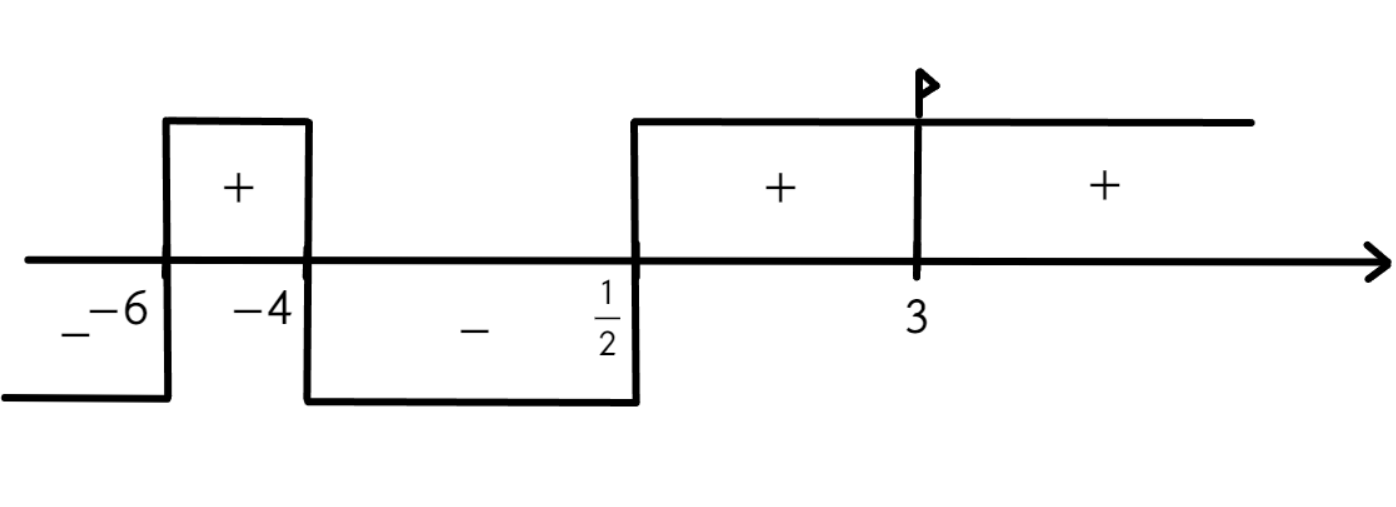
\includegraphics[scale=0.35]{int82.png}}
\end{figure}
$x\in(-\infty;-6)\cup\left[-4;\cfrac{1}{2}\right]\cup\{3\}.$\newpage\noindent
83. $\cfrac{(2x^2+5x-3)(x-4)^2}{x+5}\leqslant0\Leftrightarrow\cfrac{(2x-1)(x+3)(x-4)^2}{x+5}\leqslant0.$
Применив метод интервалов, найдём ответ:
\begin{figure}[ht!]
\center{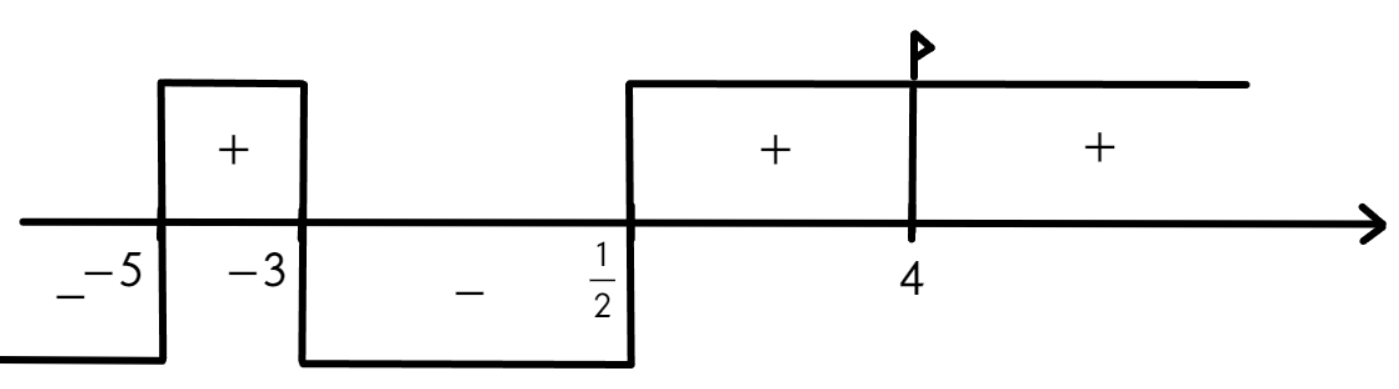
\includegraphics[scale=0.35]{int83.png}}
\end{figure}
$x\in(-\infty;-5)\cup\left[-3;\cfrac{1}{2}\right]\cup\{4\}.$\\
84. $\begin{cases} x^2+3x-4\geqslant0,\\ -x-5<0.\end{cases}\Leftrightarrow \begin{cases} (x+4)(x-1)\geqslant0,\\ x>-5.\end{cases}
\Leftrightarrow \begin{cases} x\in(-\infty;-4]\cup[1;+\infty),\\ x>-5.\end{cases}\Leftrightarrow x\in(-5;-4]\cup[1;+\infty).$\\
85. $\begin{cases} x^2+2x-3\leqslant0,\\ -x-1>0.\end{cases} \Leftrightarrow\begin{cases} (x+3)(x-1)\leqslant0,\\ x<-1.\end{cases}
\Leftrightarrow\begin{cases} x\in[-3;1],\\ x<-1.\end{cases}\Leftrightarrow x\in[-3;-1).$\\
86. $2|x-1|\geqslant 2-x\Leftrightarrow |x-1|\geqslant \cfrac{2-x}{2} \Leftrightarrow \left[\begin{array}{l} x-1\geqslant \cfrac{2-x}{2},\\
x-1\leqslant \cfrac{x-2}{2}\end{array}\right. \Leftrightarrow \left[\begin{array}{l} 2x-2-2+x\geqslant 0,\\
2x-2-x+2\leqslant 0.\end{array}\right. \Leftrightarrow \left[\begin{array}{l} x\geqslant \cfrac{4}{3},\\
x\leqslant 0.\end{array}\right. $\\$\Leftrightarrow x\in(-\infty;0]\cup\left[\cfrac{4}{3};+\infty\right).$\\
87. $2|x+1|\geqslant x+2\Leftrightarrow |x+1|\geqslant \cfrac{x+2}{2} \Leftrightarrow \left[\begin{array}{l} x+1\geqslant \cfrac{x+2}{2},\\
x+1\leqslant \cfrac{-x-2}{2}.\end{array}\right. \Leftrightarrow \left[\begin{array}{l} 2x+2-2-x\geqslant 0,\\
2x+2+x+2\leqslant 0.\end{array}\right. \Leftrightarrow \left[\begin{array}{l} x\geqslant 0,\\
x\leqslant -\cfrac{4}{3}.\end{array}\right.$\\$ \Leftrightarrow x\in\left(-\infty;-\cfrac{4}{3}\right]\cup[0;+\infty).$\\
88. $\cfrac{2|x-1|}{2-x}\geqslant1 \Leftrightarrow \cfrac{2|x-1|+x-2}{2-x}\geqslant0\Leftrightarrow
\left[\begin{array}{l}\begin{cases} \cfrac{2x-2+x-2}{2-x}\geqslant0,\\ x\geqslant 1.\end{cases}\\ \begin{cases}\cfrac{-2x+2+x-2}{2-x}\geqslant0,\\ x<1.           \end{cases}\end{array}\right.\Leftrightarrow
\left[\begin{array}{l}\begin{cases} \cfrac{3x-4}{2-x}\geqslant0,\\ x\geqslant 1.\end{cases}\\ \begin{cases}\cfrac{-x}{2-x}\geqslant0,\\ x<1.           \end{cases}\end{array}\right.\Leftrightarrow
\left[\begin{array}{l}\begin{cases} x\in\left[\cfrac{4}{3};2\right),\\ x\geqslant 1.\end{cases}\\ \begin{cases}x\in(-\infty;0]\cup(2;+\infty),\\ x<1.           \end{cases}\end{array}\right.\Leftrightarrow x\in(-\infty;0]\cup\left[\cfrac{4}{3};2\right).$\\
89. $\cfrac{2|x+1|}{x+2}\geqslant1 \Leftrightarrow \cfrac{2|x+1|-x-2}{x+2}\geqslant0\Leftrightarrow
\left[\begin{array}{l}\begin{cases} \cfrac{2x+2-x-2}{x+2}\geqslant0,\\ x\geqslant -1.\end{cases}\\ \begin{cases}\cfrac{-2x-2-x-2}{x+2}\geqslant0,\\ x<-1.           \end{cases}\end{array}\right.\Leftrightarrow
\left[\begin{array}{l}\begin{cases} \cfrac{x}{x+2}\geqslant0,\\ x\geqslant -1.\end{cases}\\ \begin{cases}\cfrac{-3x-4}{x+2}\geqslant0,\\ x<-1.           \end{cases}\end{array}\right.\Leftrightarrow
\left[\begin{array}{l}\begin{cases} x\in(-\infty;-2)\cup[0;+\infty),\\ x\geqslant -1.\end{cases}\\ \begin{cases}x\in\left(-2;-\cfrac{4}{3}\right],\\ x<-1.\end{cases}\end{array}\right.\Leftrightarrow x\in\left(-2;-\cfrac{4}{3}\right]\cup[0;+\infty).$\\
90. $\begin{cases} |x^2+2x-15|\leqslant0,\\ x^{15}-3x^{14}+2x-5>0.\end{cases}$ Модуль может не превосходить 0 только если он равен нулю, значит $x^2+2x-15=0,\
(x+5)(x-3)=0,\ x=-5$ или $x=3.$ Надо проверить, удовлетворяют ли найденные значения второму неравенству, для этого преобразуем его: $x^{15}-3x^{14}+2x-5=x^{14}(x-3)+(2x-5)>0.$ При $x=3$ левая часть равна 1, а при $x=-5$ она будет отрицательна, значит решением является только $x=3.$\\
91. $-2<\cfrac{1-x}{x}<3\Leftrightarrow \begin{cases} \cfrac{1-x}{x}+2>0,\\ \cfrac{1-x}{x}-3<0.\end{cases}\Leftrightarrow
\begin{cases} \cfrac{1+x}{x}>0,\\ \cfrac{1-4x}{x}<0.\end{cases}\Leftrightarrow \begin{cases} x\in(-\infty;-1)\cup(0;+\infty),\\ x\in (-\infty;0)\cup\left(\cfrac{1}{4};+\infty\right)\end{cases}\Leftrightarrow$\\$ x\in(-\infty;-1)\cup\left(\cfrac{1}{4};+\infty\right).$\\
92. $x\cdot|x^2-5x|\leqslant6x \Leftrightarrow \left[\begin{array}{l} \begin{cases} |x^2-5x|\leqslant6,\\ x>0.\end{cases}\\
\begin{cases} |x^2-5x|\geqslant6,\\ x<0.\end{cases}\\x=0.\end{array}\right.
\Leftrightarrow \left[\begin{array}{l} \begin{cases} x^2-5x\leqslant6,\\ x^2-5x\geqslant-6,\\ x>0.\end{cases}\\
\begin{cases} \left[\begin{array}{l}x^2-5x\geqslant6,\\ x^2-5x\leqslant-6,\end{array}\right.\\ x<0.\end{cases}\\x=0.\end{array}\right.
\Leftrightarrow$\\$ \left[\begin{array}{l} \begin{cases} (x-6)(x+1)\leqslant0,\\ (x-2)(x-3)\geqslant0,\\ x>0.\end{cases}\\
\begin{cases} \left[\begin{array}{l}(x-6)(x+1)\geqslant0,\\ (x-2)(x-3)\leqslant0,\end{array}\right.\\ x<0.\end{cases}\\x=0.\end{array}\right.$
$\Leftrightarrow\left[\begin{array}{l} \begin{cases} x\in[-1;6],\\ x\in(-\infty;2]\cup[3;+\infty),\\ x>0.\end{cases}\\
\begin{cases} \left[\begin{array}{l}x\in(-\infty;-1]\cup[6;+\infty),\\ x\in[2;3],\end{array}\right.\\ x<0.\end{cases}\\x=0.\end{array}\right.
\Leftrightarrow\left[\begin{array}{l} x\in(0;2]\cup[3;6],\\
x\in(-\infty;-1],\\x=0.\end{array}\right.\Leftrightarrow $\\$x \in (-\infty;-1]\cup[0;2]\cup[3;6].$\\
93. $\cfrac{3}{5x-1}+\cfrac{4}{3x+1}\geqslant1\Leftrightarrow\cfrac{9x+3+20x-4-15x^2-5x+3x+1}{(5x-1)(3x+1)}\geqslant 0\Leftrightarrow
\cfrac{3x(9-5x)}{(5x-1)(3x+1)}\geqslant 0.$ Применив метод интервалов, найдём ответ:
\begin{figure}[ht!]
\center{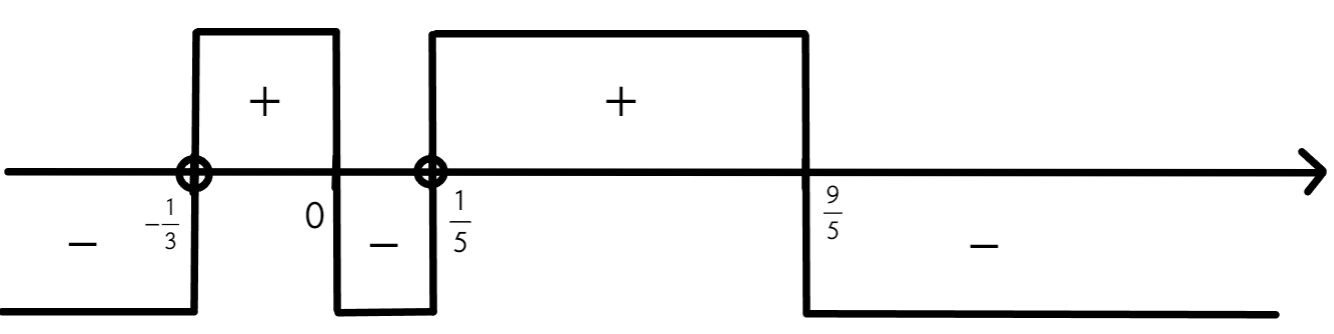
\includegraphics[scale=0.35]{int93.png}}
\end{figure}
$x\in\left(-\cfrac{1}{3};0\right]\cup\left(\cfrac{1}{5};\cfrac{9}{5}\right].$\newpage\noindent
94. $\cfrac{5}{2x+1}+\cfrac{2}{7x-1}\leqslant3\Leftrightarrow\cfrac{35x-5+4x+2-42x^2+6x-21x+3}{(2x+1)(7x-1)}\leqslant 0\Leftrightarrow
\cfrac{6x(4-7x)}{(2x+1)(7x-1)}\leqslant 0.$ Применив метод интервалов, найдём ответ:
\begin{figure}[ht!]
\center{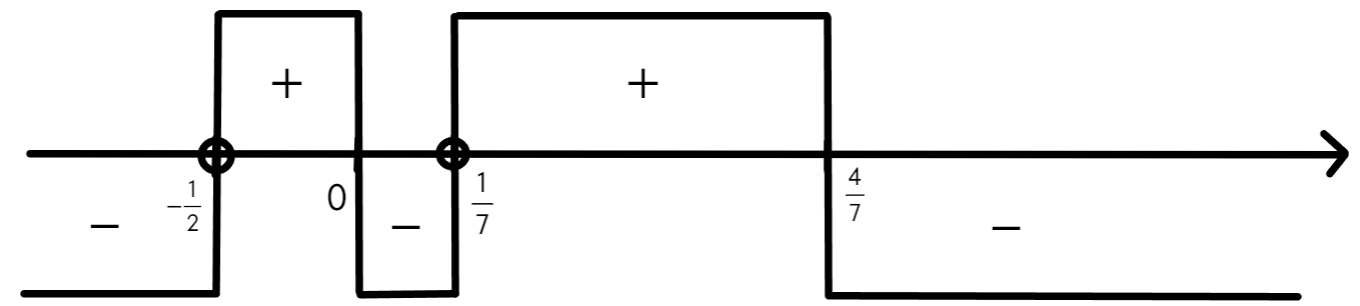
\includegraphics[scale=0.35]{int94.png}}
\end{figure}
$x\in\left(-\infty;-\cfrac{1}{2}\right)\cup\left[0;\cfrac{1}{7}\right)\cup\left(\cfrac{4}{7};+\infty\right).$\\
95. $\cfrac{(x^2-3x+2)(1-x)}{x-3}\geqslant0\Leftrightarrow\cfrac{(x-2)(x-1)(1-x)}{x-3}\geqslant0\Leftrightarrow\cfrac{(x-2)(x-1)^2}{x-3}\leqslant0.$ Применив метод интервалов, найдём ответ:
\begin{figure}[ht!]
\center{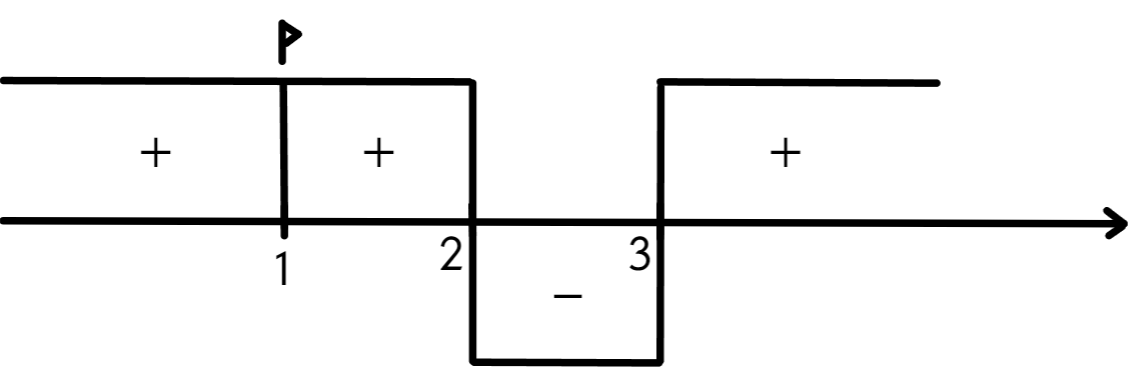
\includegraphics[scale=0.35]{int95.png}}
\end{figure}
$x\in\{1\}\cup[2;3).$\\
96. $\cfrac{3x^3}{x-5}\geqslant\cfrac{-2x^2}{5-x}\Leftrightarrow\cfrac{3x^3}{x-5}\geqslant\cfrac{2x^2}{x-5}\Leftrightarrow
\cfrac{3x^3-2x^2}{x-5}\geqslant0\Leftrightarrow\cfrac{x^2(3x-2)}{x-5}\geqslant0.$ Применив метод интервалов, найдём ответ: $x\in\left(-\infty;\cfrac{2}{3}\right]
\cup(5;+\infty).$
\begin{figure}[ht!]
\center{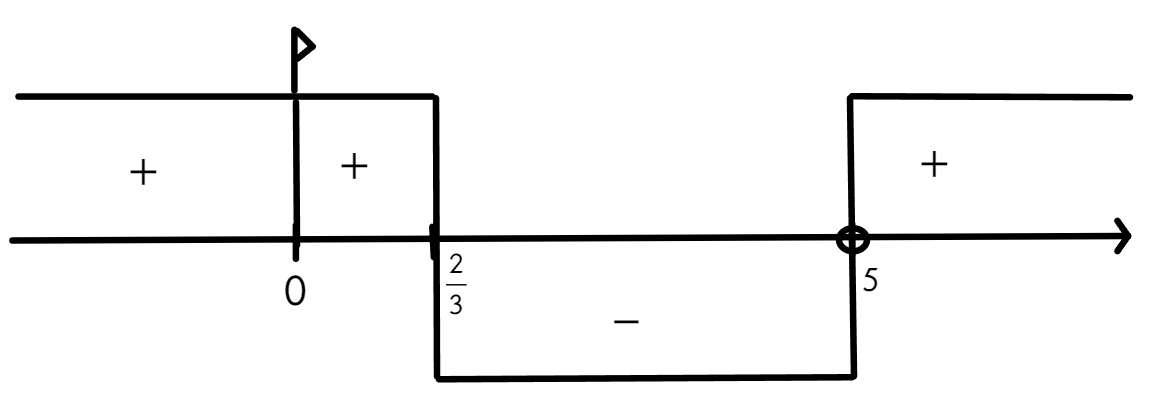
\includegraphics[scale=0.35]{ner30-1.png}}
\end{figure}\\
97. $|x+2|+|x-2|\leqslant2x\Leftrightarrow\left[\begin{array}{l}\begin{cases}-x-2-x+2\leqslant2x,\\ x\leqslant-2\end{cases}\\
\begin{cases}x+2-x+2\leqslant2x,\\ -2\leqslant x \leqslant 2\end{cases}\\
\begin{cases}x+2+x-2\leqslant2x,\\ 2\leqslant x \end{cases}
\end{array}\right.\Leftrightarrow\left[\begin{array}{l}\begin{cases}-4x\leqslant0,\\ x\leqslant-2\end{cases}\\
\begin{cases}4\leqslant2x,\\ -2\leqslant x \leqslant 2\end{cases}\\
\begin{cases}0\leqslant0,\\ 2\leqslant x \end{cases}
\end{array}\right.\Leftrightarrow x\in[2;+\infty).$\newpage\noindent
98. $\cfrac{(x-7)\sqrt{x+5}}{x^6-16x^2}\geqslant0\Leftrightarrow
\cfrac{(x-7)\sqrt{x+5}}{x^2(x-2)(x+2)(x^2+4)}\geqslant0.$ Применив метод интервалов, найдём ответ: $x\in\{-5\}\cup(-2;0)\cup(0;2)\cup[7;+\infty).$
\begin{figure}[ht!]
\center{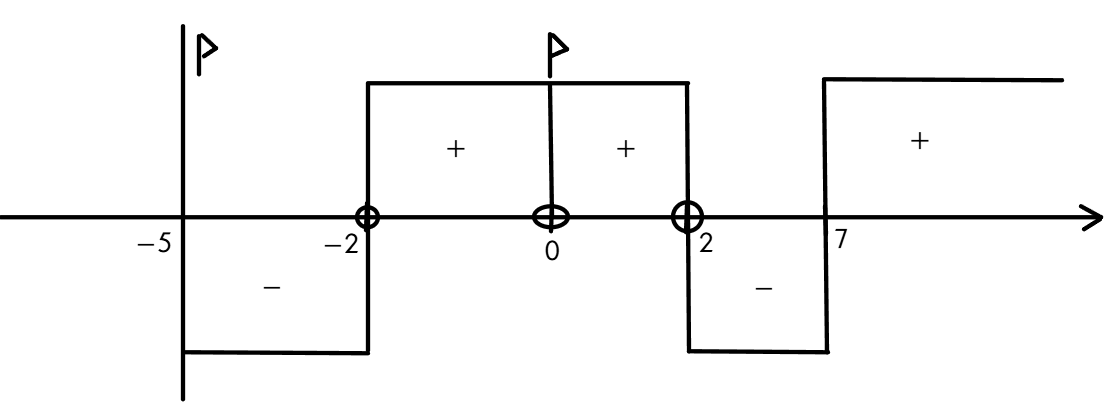
\includegraphics[scale=0.35]{int97.png}}
\end{figure}\\
99. $\cfrac{(x-5)\sqrt{x+7}}{x^6-81x^2}\geqslant0\Leftrightarrow
\cfrac{(x-5)\sqrt{x+7}}{x^2(x-3)(x+3)(x^2+9)}\geqslant0.$ Применив метод интервалов, найдём ответ: $x\in\{-7\}\cup(-3;0)\cup(0;3)\cup[5;+\infty).$
\begin{figure}[ht!]
\center{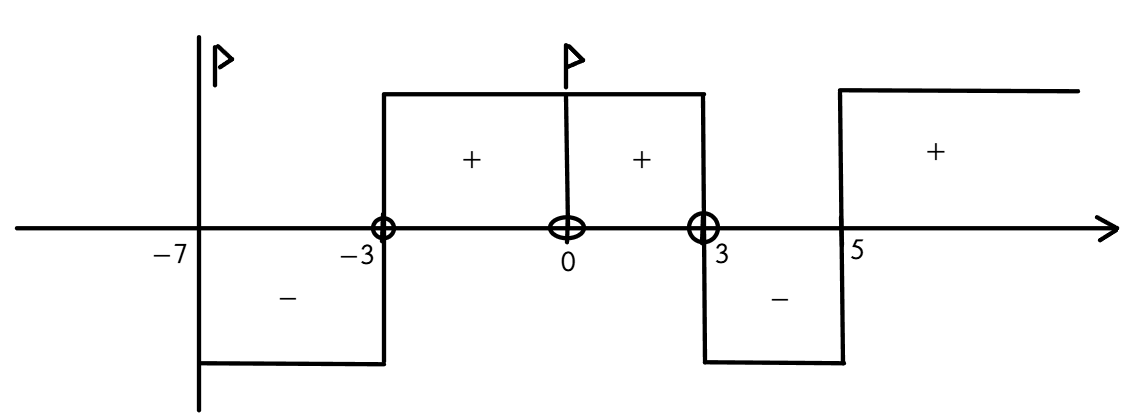
\includegraphics[scale=0.35]{int96.png}}
\end{figure}\\
100. $\cfrac{x^3-9x^2+20x}{x-4}\leqslant0\Leftrightarrow \cfrac{x(x^2-9x+20)}{x-4}\leqslant0\Leftrightarrow\cfrac{x(x-4)(x-5)}{x-4}\leqslant0.$ Применив метод интервалов, найдём ответ: $x\in[0;4)\cup(4;5].$
\begin{figure}[ht!]
\center{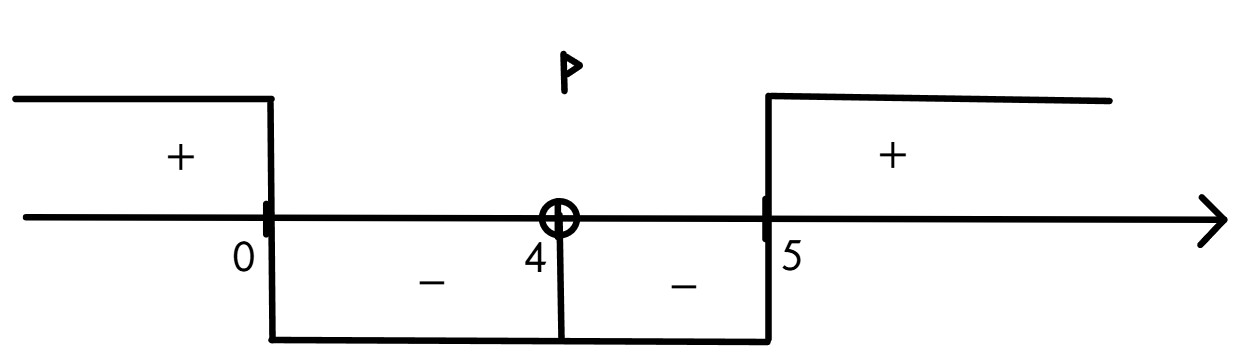
\includegraphics[scale=0.35]{int85.png}}
\end{figure}\\
101. $\cfrac{x^3-8x^2+15x}{x-3}\leqslant0\Leftrightarrow \cfrac{x(x^2-8x+15)}{x-3}\leqslant0\Leftrightarrow\cfrac{x(x-3)(x-5)}{x-3}\leqslant0.$ Применив метод интервалов, найдём ответ: $x\in[0;3)\cup(3;5].$
\begin{figure}[ht!]
\center{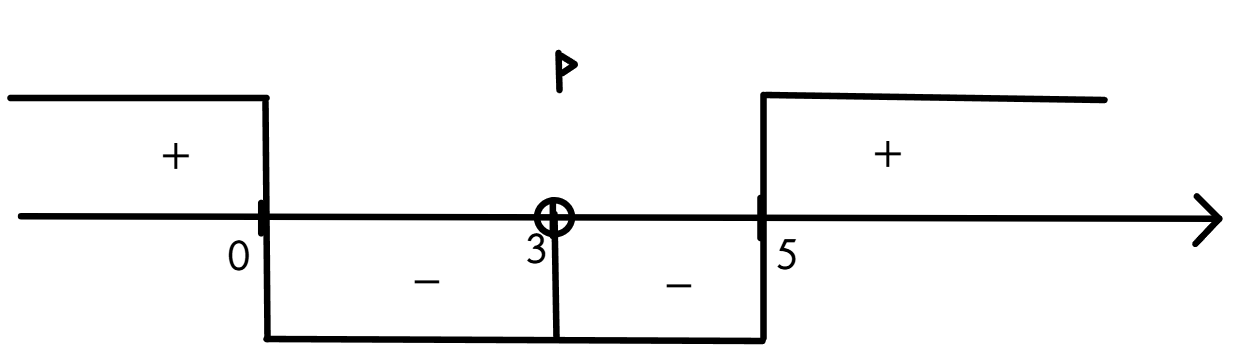
\includegraphics[scale=0.35]{int84.png}}
\end{figure}
\newpage
\section{Исследование функций и уравнений решения}
1. По теореме Виета $x_1+x_2=4,\ x_1x_2=a.$ Тогда $x_1^2+x_2^2=(x_1+x_2)^2-2x_1x_2=16-2a=16\Rightarrow a=0.$ Дискриминант уравнения в этом случае равен 16, а значит корни существуют и $a=0$ является ответом.\\
2. По теореме Виета $x_1+x_2=2,\ x_1x_2=a.$ Тогда $(x_1-x_2)^2=(x_1+x_2)^2-4x_1x_2=4-4a=16\Rightarrow a=-3.$ Дискриминант уравнения в этом случае равен 16, а значит корни существуют и $a=-3$ является ответом.\\
3. Для нахождения области определения данной функции необходимо решить неравенство\\ $\cfrac{|x-3|(x+4)(x^2+9x+20)}{x^2-x-6}\geqslant0\Leftrightarrow
\cfrac{|x-3|(x+4)^2(x+5)}{(x-3)(x+2)}\geqslant0.$ Применив метод интервалов, найдём ответ:
\begin{figure}[ht!]
\center{\includegraphics[scale=0.35]{isl3.png}}
\end{figure}
$x\in[-5;-2)\cup(3;+\infty).$\\
4. Для нахождения области определения данной функции необходимо решить неравенство\\ $\cfrac{|x-1|(x+3)(x^2+8x+15)}{x^2+x-2}\geqslant0\Leftrightarrow
\cfrac{|x-1|(x+3)^2(x+5)}{(x-1)(x+2)}\geqslant0.$ Применив метод интервалов, найдём ответ:
\begin{figure}[ht!]
\center{\includegraphics[scale=0.35]{isl4.png}}
\end{figure}
$x\in[-5;-2)\cup(1;+\infty).$\\
5. Пусть $f(x)=ax^2+bx+c.$ Тогда $c\cdot(a+b+c)=f(0)\cdot f(1)<0.$ Значит, на концах отрезка $[0;1]$ функция $f(x)$ принимает значения разных знаков, поэтому где-то на интервале $(0;1)$ её значение равно 0. Иметь только один корень эта функция не может, так как тогда все остальные значения были бы одного знака, что невозможно. Значит, квадратный трёхчлен $ax^2+bx+c$ имеет два корня.\\
6. Пусть $f(x)=ax^2+bx+c.$ Тогда $c\cdot(a-b+c)=f(0)\cdot f(-1)<0.$ Значит, на концах отрезка $[-1;0]$ функция $f(x)$ принимает значения разных знаков, поэтому где-то на интервале $(-1;0)$ её значение равно 0. Иметь только один корень эта функция не может, так как тогда все остальные значения были бы одного знака, что невозможно. Значит, квадратный трёхчлен $ax^2+bx+c$ имеет два корня.\\
7. Возможны два случая: $D=0$ или $k-2=0.$ В первом случае $4(k-1)^2-4k(k-2)=0,\ k^2-2k+1-k^2+2k=0,\ 1=0,$ что невозможно. Во втором случае $k=2,$ что и является ответом.\\
8. Возможны два случая: $D=0$ или $k+2=0.$ В первом случае $4(k+1)^2-4k(k+2)=0,\ k^2+2k+1-k^2-2k=0,\ 1=0,$ что невозможно. Во втором случае $k=-2,$ что и является ответом.\\
9. $y=x^2-7x+6=\left(x-\cfrac{7}{2}\right)^2-\cfrac{49}{4}+6=\left(x-\cfrac{7}{2}\right)^2-\cfrac{25}{4}.$ Наименьшее значение функции достигается, когда квадрат равен 0, а наибольшее --- когда квадрат имеет наибольший модуль (в том из концов отрезка, который дальше от вершины). Значит, наименьшее значение равно $-\cfrac{25}{4},$ а наибольшее ---
$\left(8-\cfrac{7}{2}\right)^2-\cfrac{25}{4}$ или $\left(-1-\cfrac{7}{2}\right)^2-\cfrac{25}{4}.$ Оба потенциально наибольших значения равны 14.\newpage\noindent
10. Для нахождения области определения данной функции необходимо решить неравенство\\ $\cfrac{(x-1)^2(2x-x^2+2)}{(x^2+x-6)|x+2|}\geqslant0\Leftrightarrow
\cfrac{(x-1)^2(x-(1-\sqrt{3}))(x-(1+\sqrt{3}))}{(x-2)(x+3)|x+2|}\leqslant0.$ Применив метод интервалов, найдём ответ:
\begin{figure}[ht!]
\center{\includegraphics[scale=0.35]{isl10.png}}
\end{figure}
$x\in(-3;-2)\cup(-2;1-\sqrt{3}]\cup\{1\}\cup(2;1+\sqrt{3}].$\\
11. Выразим $x:\ x=4-2y.$ Тогда необходимо найти наименьшее значение выражения $(4-2y)^2-2(4-2y)y+8y^2=16-16y+4y^2-8y+4y^2+8y^2=
16y^2-24y+16=(4y-3)^2+7\geqslant7.$\\
12. Выразим $x:\ x=4+2y.$ Тогда необходимо найти наименьшее значение выражения $(4+2y)^2+2(4+2y)y+8y^2=16+16y+4y^2+8y+4y^2+8y^2=
16y^2+24y+16=(4y+3)^2+7\geqslant7.$\\
13. У этого уравнения есть корни $x=3,\ x=a$ и $x=2a.$ Корней ровно два, а не три, в том случае, если два корня совпадут. Это происходит, если $a=3,\ 2a=3$ или $2a=a.$ Решив эти уравнения, получим ответ: $a\in\{0; 1,5;3\}.$\\
14. У этого уравнения есть корни $x=5,\ x=a$ и $x=2a.$ Корней ровно два, а не три, в том случае, если два корня совпадут. Это происходит, если $a=5,\ 2a=5$ или $2a=a.$ Решив эти уравнения, получим ответ: $a\in\{0; 2,5;5\}.$\\
15. По теореме Виета $x_1+x_2=-10,\ x_1x_2=q.$ Тогда $x_1^2+x_2^2=(x_1+x_2)^2-2x_1x_2=100-2q=2\Rightarrow q=49.$ Дискриминант уравнения в этом случае равен $100-4\cdot49<0,$ а значит таких значений $q$ не существует.\\
16. По теореме Виета $x_1+x_2=10,\ x_1x_2=q.$ Тогда $x_1^2+x_2^2=(x_1+x_2)^2-2x_1x_2=100-2q=2\Rightarrow q=49.$ Дискриминант уравнения в этом случае равен $100-4\cdot49<0,$ а значит таких значений $q$ не существует.\\
17. Сначала разберём случай, когда уравнение не является квадратным: $k-1=0,\ k=1,\ -x+2=0,\ x=2.$ Теперь разберём случай, когда у уравнения один корень:
$(2k-1)^2-4\cdot2\cdot(k-1)=0,\ 4k^2-4k+1-8k+8=0,\ (2k-3)^2=0,\ k=\cfrac{3}{2}.$ В этом случае $x=\cfrac{2k-1}{2(k-1)}=\cfrac{2}{1}=2.$ Во всех остальных случаях $x=\cfrac{2k-1\pm|2k-3|}{2(k-1)}=\left[\begin{array}{l}\cfrac{2k-1+2k-3}{2(k-1)}=2,\\ \cfrac{2k-1-2k+3}{2(k-1)}=\cfrac{1}{k-1}.\end{array}\right.$\\
18. Сначала разберём случай, когда уравнение не является квадратным: $k-1=0,\ k=1,\ x-2=0,\ x=2.$ Теперь разберём случай, когда у уравнения один корень:
$(2k-3)^2+4\cdot2\cdot(k-1)=0,\ 4k^2-12k+9+8k-8=0,\ (2k-1)^2=0,\ k=\cfrac{1}{2}.$ В этом случае $x=\cfrac{2k-3}{2(k-1)}=\cfrac{-2}{-1}=2.$ Во всех остальных случаях $x=\cfrac{2k-3\pm|2k-1|}{2(k-1)}=\left[\begin{array}{l}\cfrac{2k-3+2k-1}{2(k-1)}=2,\\ \cfrac{2k-3-2k+1}{2(k-1)}=\cfrac{1}{1-k}.\end{array}\right.$\\
19. По теореме Виета $x_1+x_2=\cfrac{3}{2},\ x_1x_2=-\cfrac{11}{2}.$ Тогда $\cfrac{x_1}{x_2}+\cfrac{x_2}{x_1}=\cfrac{x_1^2+x_2^2}{x_1x_2}=
\cfrac{(x_1+x_2)^2-2x_1x_2}{x_1x_2}=\cfrac{\cfrac{9}{4}+2\cdot\cfrac{11}{2}}{-\cfrac{11}{2}}=-\cfrac{53}{22}.$\\
20. По теореме Виета $x_1+x_2=-\cfrac{3}{2},\ x_1x_2=-\cfrac{11}{2}.$ Тогда $\cfrac{x_1}{x_2}+\cfrac{x_2}{x_1}=\cfrac{x_1^2+x_2^2}{x_1x_2}=
\cfrac{(x_1+x_2)^2-2x_1x_2}{x_1x_2}=\cfrac{\cfrac{9}{4}+2\cdot\cfrac{11}{2}}{-\cfrac{11}{2}}=-\cfrac{53}{22}.$\\
21. Выразим $x:\ x=3-\cfrac{3}{2}y.$ Тогда $xy=\left(3-\cfrac{3}{2}y\right)y=3y-\cfrac{3}{2}y^2=-\cfrac{3}{2}(y^2-2y)=
-\cfrac{3}{2}((y-1)^2-1)=-\cfrac{3}{2}(y-1)^2+\cfrac{3}{2}\leqslant\cfrac{3}{2}.$\\
22. Выразим $y:\ y=3-\cfrac{3}{2}x.$ Тогда $xy=\left(3-\cfrac{3}{2}x\right)x=3x-\cfrac{3}{2}x^2=-\cfrac{3}{2}(x^2-2x)=
-\cfrac{3}{2}((x-1)^2-1)=-\cfrac{3}{2}(x-1)^2+\cfrac{3}{2}\leqslant\cfrac{3}{2}.$\\
23. Пусть $x_1=2x_2,$ тогда $x_1+x_2=3x_2=k+4$ по теореме Виета. Значит, $x_2=\cfrac{k+4}{3}$ является корнем уравнения, подставим его:
$\left(\cfrac{k+4}{3}\right)^2-\cfrac{(k+4)^2}{3}+2k+4=0,\ \cfrac{k^2+8k+16}{9}-\cfrac{(k+4)^2}{3}+2k+4=0,\ k^2+8k+16-3k^2-24k-48+18k+36=0,\
2k^2-2k+4=0,\ k^2-k+2=0,\ (k+1)(k-2)=0,\ k=-1$ или $k=2.$ Рассмотренное нами условие являлось необходимым, но не достаточным, так что найденные значения $k$ необходимо проверить. При $k=-1:\ x^2-3x+2=0,$ корни $x=2$ и $x=1,$ значит $k=-1$ подходит. При $k=2:\ x^2-6x+8=0,$ корни $x=2$ и $x=4,$ значит $k=2$ также подходит.\\
24. Пусть $x_1=2x_2,$ тогда $x_1+x_2=3x_2=k+5$ по теореме Виета. Значит, $x_2=\cfrac{k+5}{3}$ является корнем уравнения, подставим его:
$\left(\cfrac{k+5}{3}\right)^2-\cfrac{(k+5)^2}{3}+2k+6=0,\ \cfrac{k^2+10k+25}{9}-\cfrac{(k+5)^2}{3}+2k+6=0,\ k^2+10k+25-3k^2-30k-75+18k+54=0,\
2k^2+2k-4=0,\ k^2+k-2=0,\ (k+2)(k-1)=0,\ k=-2$ или $k=1.$ Рассмотренное нами условие являлось необходимым, но не достаточным, так что найденные значения $k$ необходимо проверить. При $k=-2:\ x^2-3x+2=0,$ корни $x=2$ и $x=1,$ значит $k=-2$ подходит. При $k=1:\ x^2-6x+8=0,$ корни $x=2$ и $x=4,$ значит $k=1$ также подходит.\\
25. $\cfrac{x^2-4ax+3a^2}{x-3}=0\Leftrightarrow\cfrac{(x-3a)(x-a)}{x-3}=0\Leftrightarrow\begin{cases}\left[\begin{array}{l}x=3a,\\ x=a.\end{array}\right.\\x\neq3.\end{cases}$ У этого уравнения ровно один корень, если его корни совпадают (и не совпадают с 3) или если один из его корней совпадает с 3. В первом случае $a=3a,\ a=0, x=0.$ Во втором случае может быть $a=3$ или $3a=3,\ a=1.$\\
26. $\cfrac{x^2-5ax+4a^2}{x-4}=0\Leftrightarrow\cfrac{(x-4a)(x-a)}{x-4}=0\Leftrightarrow\begin{cases}\left[\begin{array}{l}x=4a,\\ x=a.\end{array}\right.\\x\neq4.\end{cases}$ У этого уравнения ровно один корень, если его корни совпадают (и не совпадают с 4) или если один из его корней совпадает с 4. В первом случае $a=4a,\ a=0, x=0.$ Во втором случае может быть $a=4$ или $4a=4,\ a=1.$\\
27. По теореме Виета $x_1+x_2=a,\ x_1x_2=20.$ Тогда $x_1^2+x_2^2=(x_1+x_2)^2-2x_1x_2=a^2-40=24\Rightarrow a=\pm8.$ Дискриминант уравнения в этом случае равен $-16$, значит подходящих значений $a$ не существует.\\
28. По теореме Виета $x_1+x_2=b,\ x_1x_2=10.$ Тогда $x_1^2+x_2^2=(x_1+x_2)^2-2x_1x_2=b^2-20=16\Rightarrow a=\pm6.$ Дискриминант уравнения в этом случае равен $-4$, значит подходящих значений $b$ не существует.\\
29. $5x^2-4x+y^2+2xy+1=x^2+2xy+y^2+4x^2-4x+1=(x+y)^2+(2x-1)^2.$ Значения квадратов всегда неотрицательны, поэтому наименьшее значение достигается при $x=\cfrac{1}{2},\ y=-x=-\cfrac{1}{2}.$\\
30. $5y^2+4y+x^2-2xy+1=x^2-2xy+y^2+4y^2+4y+1=(x-y)^2+(2y+1)^2.$ Значения квадратов всегда неотрицательны, поэтому наименьшее значение достигается при $y=-\cfrac{1}{2},\ x=y=-\cfrac{1}{2}.$\\
31. По теореме Виета $x_1+x_2=q,\ x_1x_2=4.$ Тогда $x_1^2+x_2^2=(x_1+x_2)^2-2x_1x_2=q^2-8=17\Rightarrow q=\pm5.$ Дискриминант уравнения в этом случае равен 9, а значит корни существуют и $q=\pm5$ является ответом.\\
32. По теореме Виета $x_1+x_2=q,\ x_1x_2=3.$ Тогда $x_1^2+x_2^2=(x_1+x_2)^2-2x_1x_2=q^2-6=10\Rightarrow q=\pm4.$ Дискриминант уравнения в этом случае равен 4, а значит корни существуют и $q=\pm4$ является ответом.\\
33. $\cfrac{(x-t)(x-2)}{x-2t}=0\Leftrightarrow\begin{cases}\left[\begin{array}{l}x=t,\\ x=2.\end{array}\right.\\x\neq2t.\end{cases}$ У этого уравнения ровно два корня, если они не совпадают друг с другом и с $2t.$ Значит, $t\neq2,\ t\neq2t$ и $2\neq2t.$ Таким образом, $t\notin\{0; 1; 2\}.$\\
34. $\cfrac{(x-t)(x-4)}{x-4t}=0\Leftrightarrow\begin{cases}\left[\begin{array}{l}x=t,\\ x=4.\end{array}\right.\\x\neq4t.\end{cases}$ У этого уравнения ровно два корня, если они не совпадают друг с другом и с $4t.$ Значит, $t\neq4,\ t\neq4t$ и $4\neq4t.$ Таким образом, $t\notin\{0; 1; 4\}.$\\
35. Возможны два случая: $D=0$ или $a+1=0.$ В первом случае $4-4(a+1)(1-a)=0,\ 1+a^2-1=0,\ a=0.$ Во втором случае $a=-1,\ x=-1.$ Значит, подходят оба значения и $a\in\{-1;0\}.$\\
36. Возможны два случая: $D=0$ или $1-a=0.$ В первом случае $4-4(a+1)(1-a)=0,\ 1+a^2-1=0,\ a=0.$ Во втором случае $a=1,\ x=1.$ Значит, подходят оба значения и $a\in\{0;1\}.$\\
37. $3x^2-2x-1=(3x+1)(x-1)=\left(3\cdot\cfrac{1-\sqrt{2}}{3}+1\right)\left(\cfrac{1-\sqrt{2}}{3}-1\right)=\cfrac{(2-\sqrt{2})(-2-\sqrt{2})}{3}=\cfrac{2-4}{3}=-\cfrac{2}{3}.$\\
38. $3x^2+2x-1=(3x-1)(x+1)=\left(3\cdot\cfrac{\sqrt{2}-1}{3}-1\right)\left(\cfrac{\sqrt{2}-1}{3}+1\right)=\cfrac{(\sqrt{2}-2)(\sqrt{2}+2)}{3}=\cfrac{2-4}{3}=-\cfrac{2}{3}.$\\
39. Так как $(1-x)(3-x)=x^2-4x+3,$ равенство будет выполняться при условии $\begin{cases}1-x\geqslant0,\\ 3-x\geqslant0.\end{cases}\Leftrightarrow x\leqslant1.$\\
40. Так как $(1-x)(5-x)=x^2-6x+5,$ равенство будет выполняться при условии $\begin{cases}1-x\geqslant0,\\ 5-x\geqslant0.\end{cases}\Leftrightarrow x\leqslant1.$\\
41. $2x^2+4xy+4y^2+3=x^2+4xy+4y^2+x^2+3=(x+2y)^2+x^2+3\geqslant3.$\\
42. $4x^2-4xy+2y^2+5=4x^2-4xy+y^2+y^2+5=(2x-y)^2+y^2+5\geqslant5.$\\
43. $\cfrac{\sqrt{x-t}}{(x-2)(x-3)}<0\Leftrightarrow \begin{cases}x>t,\\(x-2)(x-3)<0.\end{cases}
\Leftrightarrow \begin{cases}x\in(t;+\infty),\\ x\in(2;3).\end{cases}$ Полученные интервалы не пересекаются при $t\in[3;+\infty).$\\
44. $\cfrac{\sqrt{x-t}}{(x-3)(x-4)}<0\Leftrightarrow \begin{cases}x>t,\\(x-3)(x-4)<0.\end{cases}
\Leftrightarrow \begin{cases}x\in(t;+\infty),\\ x\in(3;4).\end{cases}$ Полученные интервалы не пересекаются при $t\in[4;+\infty).$\\
45. Квадратное уравнение имеет два корня при выполнении двух условий:\\ $\begin{cases}a-1\neq0,\\ D>0.\end{cases}\Leftrightarrow
\begin{cases}a\neq1,\\ 4a^2-4\cdot(a-1)\cdot4>0.\end{cases}\Leftrightarrow
\begin{cases}a\neq1,\\ (a-2)^2>0.\end{cases}\Leftrightarrow a\notin\{1;2\}.$\\
46. Квадратное уравнение имеет два корня при выполнении двух условий:\\ $\begin{cases}a+1\neq0,\\ D>0.\end{cases}\Leftrightarrow
\begin{cases}a\neq-1,\\ 4a^2+4\cdot(a+1)\cdot4>0.\end{cases}\Leftrightarrow
\begin{cases}a\neq-1,\\ (a+2)^2>0.\end{cases}\Leftrightarrow a\notin\{-2;-1\}.$\\
47. Возможны два случая: $D=0$ или $a=0.$ В первом случае $4(a+3)^2-4a(3a+3)=0, a^2+6a+9-3a^2-3a=0, 2a^2-3a-9=0, a=3$ или $a=-\cfrac{3}{2}.$ Во втором случае $a=0,\ x=\cfrac{1}{2}.$ Значит, подходят оба случая и $a\in\left\{-\cfrac{3}{2}; 0; 3\right\}.$\\
48. Возможны два случая: $D=0$ или $k=0.$ В первом случае $4(k+1)^2-4k(k+3)=0, k^2+2k+1-k^2-3k=0, k=1.$ Во втором случае $k=0,\ x=\cfrac{3}{2}.$ Значит, подходят оба случая и $k\in\{0;1\}.$\\
49. По теореме Виета $x_1+x_2=\cfrac{5}{3},\ x_1x_2=-\cfrac{11}{3}.$ Для составления искомого квадратного уравнения воспользуемся обратной теоремой Виета: обозначим $y_1=\cfrac{1}{x_1},\ y_2=\cfrac{1}{x_2}$ и найдём $y_1+y_2$ и $y_1y_2:\ y_1+y_2=\cfrac{1}{x_1}+\cfrac{1}{x_2}=
\cfrac{x_1+x_2}{x_1x_2}=\cfrac{\cfrac{5}{3}}{-\cfrac{11}{3}}=-\cfrac{5}{11}=-\cfrac{b}{a},\ y_1y_2=\cfrac{1}{x_1x_2}=\cfrac{1}{-\cfrac{11}{3}}=-\cfrac{3}{11}=\cfrac{c}{a}.$ Подойдёт, например, уравнение $11x^2+5x-3=0.$\\
50. По теореме Виета $x_1+x_2=\cfrac{3}{5},\ x_1x_2=-\cfrac{11}{5}.$ Для составления искомого квадратного уравнения воспользуемся обратной теоремой Виета: обозначим $y_1=\cfrac{1}{x_1},\ y_2=\cfrac{1}{x_2}$ и найдём $y_1+y_2$ и $y_1y_2:\ y_1+y_2=\cfrac{1}{x_1}+\cfrac{1}{x_2}=
\cfrac{x_1+x_2}{x_1x_2}=\cfrac{\cfrac{3}{5}}{-\cfrac{11}{5}}=-\cfrac{3}{11}=-\cfrac{b}{a},\ y_1y_2=\cfrac{1}{x_1x_2}=\cfrac{1}{-\cfrac{11}{5}}=-\cfrac{5}{11}=\cfrac{c}{a}.$ Подойдёт, например, уравнение $11x^2+3x-5=0.$\\
51. $x^4-3x^2-4=(x^2-4)(x^2+1)=(x-2)(x+2)(x^2+1)=0.$ Произведение вещественных корней равно $2\cdot(-2)=-4.$\\
52. $x^4+3x^2-4=(x^2+4)(x^2-1)=(x^2+4)(x-1)(x+1)=0.$ Произведение вещественных корней равно $1\cdot(-1)=-1.$\\
53. Квадратное уравнение имеет два корня при выполнении двух условий:\\ $\begin{cases}a\neq0,\\ D>0.\end{cases}\Leftrightarrow
\begin{cases}a\neq0,\\ 16-4\cdot a \cdot a>0.\end{cases}\Leftrightarrow
\begin{cases}a\neq0,\\ (2-a)(2+a)>0.\end{cases}\Leftrightarrow a\in(-2;0)\cup(0;2).$\\
54. Квадратное уравнение имеет два корня при выполнении двух условий:\\ $\begin{cases}a\neq0,\\ D>0.\end{cases}\Leftrightarrow
\begin{cases}a\neq0,\\ 16-4\cdot a \cdot a>0.\end{cases}\Leftrightarrow
\begin{cases}a\neq0,\\ (2-a)(2+a)>0.\end{cases}\Leftrightarrow a\in(-2;0)\cup(0;2).$\\
55. $\cfrac{(x-t)(x-2t)}{x-1}=0\Leftrightarrow\begin{cases}\left[\begin{array}{l}x=t,\\ x=2t.\end{array}\right.\\x\neq1.\end{cases}$
У этого уравнения ровно два корня, если они не совпадают друг с другом и с $1.$ Значит, $t\neq2t\ (t=0),\ t\neq1$ и $2t\neq1.$ Таким образом, $t\notin\left\{0; \cfrac{1}{2}; 1\right\}.$\\
56. $\cfrac{(x-t)(x-2t)}{x-2}=0\Leftrightarrow\begin{cases}\left[\begin{array}{l}x=t,\\ x=2t.\end{array}\right.\\x\neq2.\end{cases}$
У этого уравнения ровно два корня, если они не совпадают друг с другом и с $2.$ Значит, $t\neq2t\ (t=0),\ t\neq2$ и $2t\neq2.$ Таким образом, $t\notin\left\{0; 1; 2\right\}.$\\
57. $4x_1^2+8x_1-7=2(2x_1^2+4x_1-5)+3=3.$\\
58. $6x_1^2+4x_1-11=2(3x_1^2+2x_1-7)+3=3.$\\
59. $x^2-12x+15=(x+a)^2+b,\ x^2-12x+15=x^2+2ax+a^2+b.$ Значит, $2a=-12,\ a=-6,$ а $b=15-a^2=-21.$\\
60. $x^2-8x-3=(x+a)^2+b,\ x^2-8x-3=x^2+2ax+a^2+b.$ Значит, $2a=-8,\ a=-4,$ а $b=-3-a^2=-19.$\\
61. По теореме Виета $x_1+x_2=-p,\ x_1x_2=6.$ Тогда $x_1^2+x_2^2=(x_1+x_2)^2-2x_1x_2=p^2-12=37,\ p^2=49,\ p=\pm7.$ Значит, надо решить уравнение $x^2+7x+6=0$ или  $x^2-7x+6=0.$ В первом случае $(x+6)(x+1)=0,\ x=-6$ или $x=-1.$ Во втором случае $(x-6)(x-1)=0,\ x=6$ или $x=1.$\\
62. По теореме Виета $x_1+x_2=p,\ x_1x_2=10.$ Тогда $x_1^2+x_2^2=(x_1+x_2)^2-2x_1x_2=p^2-20=29,\ p^2=49,\ p=\pm7.$ Значит, надо решить уравнение $x^2+7x+10=0$ или  $x^2-7x+10=0.$ В первом случае $(x+5)(x+2)=0,\ x=-5$ или $x=-2.$ Во втором случае $(x-5)(x-2)=0,\ x=5$ или $x=2.$\\
63. $x^3+6x^2+ax=0\Leftrightarrow x(x^2+6x+a)=0.$ У этого уравнения точно всегда есть корень $x=0.$ Два корня у него может быть, если один из корней уравнения
$x^2+6x+a=0$ совпадает с $x=0$ или уравнение $x^2+6x+a=0$ имеет один корень (не совпадающий с $x=0$). В первом случае $0+0+a=0,\ a=0.$ Во втором случае $D=36-4a=0,\ a=9.$ Корень $x=-3$ с корнем $x=0$ не совпадает.\\
64. $4x^3+4x^2+ax=0\Leftrightarrow x(4x^2+4x+a)=0.$ У этого уравнения точно всегда есть корень $x=0.$ Два корня у него может быть, если один из корней уравнения
$4x^2+4x+a=0$ совпадает с $x=0$ или уравнение $4x^2+4x+a=0$ имеет один корень (не совпадающий с $x=0$). В первом случае $0+0+a=0,\ a=0.$ Во втором случае $D=16-16a=0,\ a=1.$ Корень $x=-\cfrac{1}{2}$ с корнем $x=0$ не совпадает.\\
65. $\begin{cases} y=x^2-4x+3,\\ y=a.\end{cases}\Leftrightarrow
\begin{cases} x^2-4x+3-a=0,\\ y=a.\end{cases}$ Система имеет единственное решение, когда единственное решение имеет уравнение $x^2-4x+3-a=0.$ Для этого необходимо и достаточно, чтобы $D=16-4(3-a)=4+4a=0,\ a=-1.$\\
66. $\begin{cases} y=x^2+4x+3,\\ y=a.\end{cases}\Leftrightarrow
\begin{cases} x^2+4x+3-a=0,\\ y=a.\end{cases}$ Система имеет единственное решение, когда единственное решение имеет уравнение $x^2+4x+3-a=0.$ Для этого необходимо и достаточно, чтобы $D=16-4(3-a)=4+4a=0,\ a=-1.$\\
67. Корни существуют, так как $D=81-80=1>0.$ По теореме Виета $x_1+x_2=-9,\ x_1x_2=20,$ значит $x_1^2+x_2^2=(x_1+x_2)^2-2x_1x_2=81-40=41.$\\
68. Выразим $x:\ x=2y+4.$ Тогда $(2y+4)^2-2(2y+4)y+8y^2=4y^2+16y+16-4y^2-8y+8y^2=8y^2+8y+16=8(y^2+y+2)=8\left(\left(y+\cfrac{1}{2}\right)^2+\cfrac{7}{4}\right)\geqslant8\cdot\cfrac{7}{4}=14.$\newpage
\noindent69. Для нахождения области определения функции необходимо решить неравенство $\cfrac{x^2+8x+15}{x-2}\geqslant0\Leftrightarrow
\cfrac{(x+3)(x+5)}{x-2}\geqslant0.$ Применив метод интервалов, найдём ответ:
\begin{figure}[ht!]
\center{\includegraphics[scale=0.35]{isl69.png}}
\end{figure}
$x\in[-5;-3]\cup(2;+\infty).$\\
70. Необходимо выполнение двух условий: $\begin{cases} x^2-6x+8\geqslant0,\\ x-5\neq0.\end{cases}\Leftrightarrow
\begin{cases} (x-2)(x-4)\geqslant0,\\ x-5\neq0.\end{cases}
\Leftrightarrow$\\$ x\in (-\infty;2]\cup[4;5)\cup(5;+\infty).$\\
71. Необходимо выполнение двух условий: $\begin{cases} x^2-7x+12\geqslant0,\\ x-6\neq0.\end{cases}\Leftrightarrow
\begin{cases} (x-3)(x-4)\geqslant0,\\ x-6\neq0.\end{cases}
\Leftrightarrow$\\$ x\in (-\infty;3]\cup[4;6)\cup(6;+\infty).$\\
72. Уравнение имеет только положительные корни при выполнении следующих условий: эти корни существуют (то есть $D\geqslant0),$ их сумма и произведение положительны (эти условия мы будем проверять при помощи теоремы Виета). Запишем эти условия в виде системы неравенств и решим её: $\begin{cases} 4-4\cdot7\cdot4k\geqslant0,\\
\cfrac{2}{7}>0,\\ \cfrac{4k}{7}>0.\end{cases}\Leftrightarrow\begin{cases} k\leqslant\cfrac{1}{28},\\ k>0\end{cases}\Leftrightarrow
k\in \left(0;\cfrac{1}{28}\right].$\\
73. Уравнение имеет только положительные корни при выполнении следующих условий: эти корни существуют (то есть $D\geqslant0),$ их сумма и произведение положительны (эти условия мы будем проверять при помощи теоремы Виета). Запишем эти условия в виде системы неравенств и решим её: $\begin{cases} 4-4\cdot3\cdot9k\geqslant0,\\
\cfrac{2}{3}>0,\\ \cfrac{9k}{3}>0.\end{cases}\Leftrightarrow\begin{cases} k\leqslant\cfrac{1}{27},\\ k>0\end{cases}\Leftrightarrow
k\in \left(0;\cfrac{1}{27}\right].$\\
74. Выразим $y:\ y=3-\cfrac{3}{2}x.$ Если $x\in(-8;8),$ то $\cfrac{3}{2}x\in (-12;12),\ 3-\cfrac{3}{2}x\in (-9;15).$\\
75. Выразим $x:\ x=2-\cfrac{3}{4}y.$ Если $y\in(-12;12),$ то $\cfrac{3}{4}y\in (-9;9),\ 2-\cfrac{3}{4}y\in (-7;11).$\\
76. Для того, чтобы число 1 находилось между корнями уравнения, необходимо и достаточно выполнение двух условий. Во-первых, эти корней должно быть два, то есть $D>0.$ Во-вторых, выражение $(x_1-1)(x_2-1)$ должно быть отрицательно (это гарантирует, что скобки разных знаков, а значит один корень больше 1, а другой меньше). Запишем эти условия в виде системы неравенств и решим её, воспользовавшись теоремой Виета:\\
$\begin{cases}(a+1)^2+4a^2>0,\\ (x_1-1)(x_2-1)<0.\end{cases}\Leftrightarrow x_1x_2-(x_1+x_2)+1<0\Leftrightarrow
-a^2+a+1+1<0\Leftrightarrow a^2-a-2>0\Leftrightarrow (a-2)(a+1)>0\Leftrightarrow a\in (-\infty;-1)\cup(2;+\infty).$\\
77. Для того, чтобы число 1 находилось между корнями уравнения, необходимо и достаточно выполнение двух условий. Во-первых, эти корней должно быть два, то есть $D>0.$ Во-вторых, выражение $(x_1-1)(x_2-1)$ должно быть отрицательно (это гарантирует, что скобки разных знаков, а значит один корень больше 1, а другой меньше). Запишем эти условия в виде системы неравенств и решим её, воспользовавшись теоремой Виета:\\
$\begin{cases}(1-a)^2+4a^2>0,\\ (x_1-1)(x_2-1)<0.\end{cases}\Leftrightarrow x_1x_2-(x_1+x_2)+1<0\Leftrightarrow
-a^2+1-a+1<0\Leftrightarrow a^2+a-2>0\Leftrightarrow (a+2)(a-1)>0\Leftrightarrow a\in (-\infty;-2)\cup(1;+\infty).$\\
78. По теореме Виета $x_1+x_2=15,\ x_1x_2=q.$ Тогда $\cfrac{1}{x_1}+\cfrac{1}{x_2}=\cfrac{x_1+x_2}{x_1x_2}=\cfrac{15}{q}=\cfrac{5}{12}\Rightarrow q=36.$ Необходимо решить уравнение $x^2-15x+36=0,\ (x-3)(x-12)=0,\ x=3$ или $x=12.$\\
79. По теореме Виета $x_1+x_2=-p,\ x_1x_2=36.$ Тогда $\cfrac{1}{x_1}+\cfrac{1}{x_2}=\cfrac{x_1+x_2}{x_1x_2}=\cfrac{-p}{36}=\cfrac{5}{12}\Rightarrow p=-15.$ Необходимо решить уравнение $x^2-15x+36=0,\ (x-3)(x-12)=0,\ x=3$ или $x=12.$\\
80. Квадратное уравнение может иметь более 2 корней только если оно вырождается в уравнение $0=0,$ которое имеет бесконечно много корней. Свободный член $4a-4$ равен нулю только при $a=1,$ при этом же значении $a$ равны нулю и остальные коэффициенты. Поэтому $a=1$ является правильным ответом.\\
81. Квадратное уравнение может иметь более 2 корней только если оно вырождается в уравнение $0=0,$ которое имеет бесконечно много корней. Свободный член $-3a+3$ равен нулю только при $a=1,$ при этом же значении $a$ равны нулю и остальные коэффициенты. Поэтому $a=1$ является правильным ответом.\\
82. По теореме Виета $x_1+x_2=4,\ x_1x_2=-1.$ Тогда $x_1^3+x_2^3=(x_1+x_2)(x_1^2-x_1x_2+x_2^2)=(x_1+x_2)((x_1+x_2)^2-3x_1x_2)=4\cdot(16+3)=76.$\\
83. По теореме Виета $x_1+x_2=3,\ x_1x_2=-2.$ Тогда $x_1^3+x_2^3=(x_1+x_2)(x_1^2-x_1x_2+x_2^2)=(x_1+x_2)((x_1+x_2)^2-3x_1x_2)=3\cdot(9+6)=45.$\\
84. Подставим значение $3:\ 27-9+3b+24=0,\ 3b=-42,\ b=-14.$ Так как 3 является корнем многочлена $x^3-x^2-14x+24,$ по теореме Безу его можно поделить на $x-3.$ Можно сделать это столбиком или схемой Горнера, но здесь мы сделаем это при помощи выделения соответствующих множителей.
$x^3-x^2-14x+24=x^2(x-3)+2x(x-3)-8(x-3)=(x-3)(x^2+2x-8)=(x-3)(x+4)(x-2)=0.$ Таким образом, $x\in\{-4; 2; 3\}.$\\
85. Подставим значение $-2:\ -8+4-2b-24=0,\ 2b=-28,\ b=-14.$ Так как $-2$ является корнем многочлена $x^3+x^2-14x-24,$ по теореме Безу его можно поделить на $x+2.$ Можно сделать это столбиком или схемой Горнера, но здесь мы сделаем это при помощи выделения соответствующих множителей.
$x^3+x^2-14x-24=x^2(x+2)-x(x+2)-12(x+2)=(x+2)(x^2-x-12)=(x+2)(x-4)(x+3).$ Таким образом, $x\in\{-3; -2; 4\}.$\\
86. $6-2x^2-2xy-6x-y^2=-(2x^2+2xy+6x+y^2-6)=-(x^2+2xy+y^2+x^2+6x+9-15)=-(x+y)^2-(x+3)^2+15.$ Наибольшее значение принимается, когда квадраты равны 0, то есть $x+3=0,\ x=-3,\ x+y=0,\ y=-x=3.$\\
87. $20-2x^2+2xy-4x-y^2=-(2x^2-2xy+y^2+4x-20)=-(x^2-2xy+y^2+x^2+4x+4-24)=-(x-y)^2-(x+2)^2+24.$ Наибольшее значение принимается, когда квадраты равны 0, то есть $x+2=0,\ x=-2,\ x-y=0,\ y=x=-2.$\\
88. Возможны два случая: $D=0$ или $a=0.$ В первом случае $4(a-2)^2-4a(a+1)=0,\ a^2-4a+4-a^2-a=0,\ a=\cfrac{4}{5}.$ Во втором случае $a=0,\ x=-\cfrac{1}{4}.$\\
89. Возможны два случая: $D=0$ или $a=0.$ В первом случае $16(a-1)^2-4a(4a-3)=0,\ 4a^2-8a+4-4a^2+3a=0,\ a=\cfrac{4}{5}.$ Во втором случае $a=0,\ x=-\cfrac{3}{4}.$\newpage\noindent
90. По теореме Виета $x_1+x_2=a^2-5a=a(a-5)<0\Leftrightarrow a\in(0;5).$ Также необходимо проверить, что корни существуют, то есть $D\geqslant0,\ (a^2-5a)^2-4\cdot4a^2=(a^2-5a-4a)(a^2-5a+4a)=a(a-9)a(a-1)=a^2(a-9)(a-1)\geqslant0.$ Применив метод интервалов, найдём ответ:
\begin{figure}[ht!]
\center{\includegraphics[scale=0.35]{isl90.png}}
\end{figure}
$a\in[-\infty;1]\cup[9;+\infty).$\\ Окончательным ответом в задаче будет пересечение полученных ответов, $a\in (0;1].$\\
91. По теореме Виета $x_1+x_2=5a-a^2=a(5-a)>0\Leftrightarrow a\in(0;5).$ Также необходимо проверить, что корни существуют, то есть $D\geqslant0,\ (a^2-5a)^2-4\cdot4a^2=(a^2-5a-4a)(a^2-5a+4a)=a(a-9)a(a-1)=a^2(a-9)(a-1)\geqslant0.$ Применив метод интервалов, найдём ответ:
\begin{figure}[ht!]
\center{\includegraphics[scale=0.35]{isl90.png}}
\end{figure}
$a\in[-\infty;1]\cup[9;+\infty).$\\ Окончательным ответом в задаче будет пересечение полученных ответов, $a\in (0;1].$\\
92. $(x-5)(2x-a)=x-5\Leftrightarrow(x-5)(2x-a-1)=0\Leftrightarrow \left[\begin{array}{l}x=5,\\ x=\cfrac{a+1}{2}.\end{array}\right.$
Если корень ровно один, то $\cfrac{a+1}{2}=5,\ a=9.$\\
93. $(x-3)(2x-a)=x-3\Leftrightarrow(x-3)(2x-a-1)=0\Leftrightarrow \left[\begin{array}{l}x=3,\\ x=\cfrac{a+1}{2}.\end{array}\right.$
Если корень ровно один, то $\cfrac{a+1}{2}=3,\ a=5.$\\
94. $ax=|x-2|\Leftrightarrow \begin{cases}\left[\begin{array}{l}x-2=ax,\\ x-2=-ax.\end{array}\right.\\ ax\geqslant0.\end{cases}\Leftrightarrow
\begin{cases}\left[\begin{array}{l}x(1-a)=2,\\ x(1+a)=2.\end{array}\right.\\ ax\geqslant0.\end{cases}$
Так как $a>0,$ корень $x=\cfrac{2}{1+a}>0$ всегда подходит. Значит, не подходить должен корень $x=\cfrac{2}{1-a}.$ Это может произойти из-за нуля в знаменателе $(a=1)$ или из-за того, что он отрицателен, то есть $1-a<0,\ a>1.$ Таким образом, при положительных $a$ уравнение имеет единственное решение при $a\in[1;+\infty).$\\
95. Необходимо выполнение системы неравенств:\\ $\begin{cases} 24-x^2\geqslant0,\\ x^2+x-20>0.\end{cases}\Leftrightarrow
\begin{cases} (2\sqrt{6}-x)(2\sqrt{6}+x)\geqslant0,\\ (x-4)(x+5)>0.\end{cases}\Leftrightarrow
\begin{cases} x\in[-2\sqrt{6};2\sqrt{6}],\\ x\in(-\infty;-5)\cup(4;+\infty).\end{cases}\Leftrightarrow x\in(4;2\sqrt{6}].$\\
96. $ax=|x+2|\Leftrightarrow \begin{cases}\left[\begin{array}{l}x+2=ax,\\ x+2=-ax.\end{array}\right.\\ ax\geqslant0.\end{cases}\Leftrightarrow
\begin{cases}\left[\begin{array}{l}x(a-1)=2,\\ x(a+1)=-2.\end{array}\right.\\ ax\geqslant0.\end{cases}$
Во-первых, один корень у этого уравнения может быть из-за того, что при вычислении второго получается 0 в знаменателе, тогда $a=1$ или $a=-1.$ При $a=1$ имеем корень $x=-1,$ который не удовлетворяет условию $ax\geqslant0,$ а при $a=-1$ --- $x=-1$ этому условию удовлетворяет. Поэтому при $a=1$ корней нет вообще, а при $a=-1$ он как раз один. При положительных значениях $a$ корень $x=-\cfrac{2}{a+1}<0,$ а значит не подходит. Поэтому должен подходить второй корень, значит $a-1>0,\ a>1.$ При отрицательных значениях $a$ корень $x=\cfrac{2}{a-1}<0$ точно подходит, значит второй корень должен не подходить. Поэтому $a+1<0,\ a<-1.$ Также корни могут совпадать, $\cfrac{2}{a-1}=-\cfrac{2}{a+1},\ a-1=-a-1,\ a=0.$ Таким образом, один корень данное уравнение имеет при $a\in(-\infty;-1]\cup\{0\}\cup(1;+\infty).$\\
97. $\begin{cases}
(k+2)x+3y=9+kx,\\
x+(k+4)y=2.
\end{cases}\Leftrightarrow\begin{cases}
2x+3y=9,\\
x+(k+4)y=2.
\end{cases}\Leftrightarrow\begin{cases}
2x+3y=9,\\
(2k+5)y=-5.
\end{cases}$
У этой системы не может быть бесконечно много решений: из второго уравнения однозначно определяется $y,$ а потом из первого уравнения определяется $x.$ Если $2k+5\neq0,$ то у системы одно решение, а при $2k+5=0$ --- ни одного.\\
98. $(ax^2+3x+1)(x-3)=(x-3)\Leftrightarrow (x-3)(ax^2+3x+1-1)=0\Leftrightarrow (x-3)x(ax+3)=0.$ У этого уравнения при любом значении $a$ точно есть решения $x=3$ и $x=0,$ значит одного решения у него быть не может.\\
99. По теореме Виета $x_1+x_2=a^2-5a=a(a-5)<0\Rightarrow a\in(0;5).$ Также необходимо проверить существование корней, то есть $D=(a^2-5a)^2-16=
(a^2-5a-4)(a^2-5a+4)=$\\$\left(a-\cfrac{5-\sqrt{41}}{2}\right)\left(a-\cfrac{5+\sqrt{41}}{2}\right)(a-4)(a-1)\geqslant0.$\\ Применив метод интервалов, найдём ответ:
\begin{figure}[ht!]
\center{\includegraphics[scale=0.35]{isl99.png}}
\end{figure}
$a\in\left(-\infty;\cfrac{5-\sqrt{41}}{2}\right]\cup[1;4]\cup\left[\cfrac{5+\sqrt{41}}{2};+\infty\right).$
Окончательным ответом в задаче будет пересечение полученных ответов, $a\in [1;4].$\\
100. По теореме Виета $x_1+x_2=\cfrac{7}{2},\ x_1x_2=2.$ Тогда $\cfrac{x_1^2}{x_2}+\cfrac{x_2^2}{x_1}=\cfrac{x_1^3+x_2^3}{x_1x_2}=\cfrac{(x_1+x_2)(x_1^2-x_1x_2+x_2^2)}{x_1x_2}=
\cfrac{(x_1+x_2)((x_1+x_2)^2-3x_1x_2)}{x_1x_2}=\cfrac{\cfrac{7}{2}\cdot\left(\cfrac{49}{4}-6\right)}{2}=\cfrac{175}{16}.$\\
101. а) Подставим $x=3:\ 7\cdot9-2\cdot3+4a=0,\ a=-\cfrac{57}{4}.$\\
б) Для этого должно выполняться неравенство $D=4-4\cdot7\cdot4a>0,\ 28a<1,\ a\in\left(-\infty;\cfrac{1}{28}\right).$\\
в) Сумма корней по теореме Виета равна $\cfrac{2}{7}>0,$ также положительно должно быть их произведение $\cfrac{4a}{7}>0,\ a>0.$ При этом корень может быть и один, поэтому в отличие от пункта б) $a=\cfrac{1}{28}$ также подходит. Таким образом, ответ $a\in\left(0;\cfrac{1}{28}\right].$\\
г) При $a<0$ согласно пункту а) корни есть, при этом их произведение отрицательно, значит среди них точно есть отрицательный. При $a=0$ корни $x=0$ и $x=\cfrac{2}{7},$ отрицательных нет. При $a\in\left(0;\cfrac{1}{28}\right]$ согласно пункту в) оба корня положительны, а при $a>\cfrac{1}{28}$ корней нет вообще, а значит нет и отрицательных. Таким образом, ответ $a\in[0;+\infty).$\\
102. а) Два корня квадратное уравнение имеет при $D=a^2-4(a-1)=(a-2)^2>0,\ a\neq2.$\\
б) Уравнение $\cfrac{x^2-ax+a-1}{x+5}=0$ имеет единственное решение либо когда уравнение $x^2-ax+a-1=0$ имеет единственное решение, отличное от $-5,$ либо когда один из корней этого уравнения равен $-5.$ По пункту а) единственное решение при $a=2,$ тогда $x=1.$ Подставим $x=-5,$ имеем $25+5a+a-1=0,\ 6a=-24,\ a=-4.$ Таким образом, $a\in\{-4;2\}.$\\
103. а) Два корня квадратное уравнение имеет при $D=a^2-4(3a-9)=(a-6)^2>0,\ a\neq6.$\\
б) Уравнение $\cfrac{x^2-ax+3a-9}{x-4}=0$ имеет единственное решение либо когда уравнение $x^2-ax+3a-9=0$ имеет единственное решение, отличное от $4,$ либо когда один из корней этого уравнения равен $4.$ По пункту а) единственное решение при $a=6,$ тогда $x=3.$ Подставим $x=4,$ имеем $16-4a+3a-9=0,\ a=7.$ Таким образом, $a\in\{6;7\}.$\\
104. Возможны два случая: $D=0$ или $a-2=0.$ В первом случае $4(a-2)^2-4(a-2)\cdot3=0,\ (a-2)(a-5)=0, a=2$ или $a=5.$ Но при $a=2$ обнуляется ещё и старший коэффициент и получается уравнение $3=0,$ корней у которого нет вообще. Таким образом, подходит только $a=5.$\\
105. Возможны два случая: $D=0$ или $a+3=0.$ В первом случае $4(a+3)^2+4(a+3)\cdot5=0,\ (a+3)(a+8)=0, a=-3$ или $a=-8.$ Но при $a=-3$ обнуляется ещё и старший коэффициент и получается уравнение $-5=0,$ корней у которого нет вообще. Таким образом, подходит только $a=-8.$\\
106. Раз график не проходит через III четверть, он пересекает ось ординат выше нуля, поэтому $b>0.$ Также при больших по модулю отрицательных значениях $x$ значения $y$ должны быть положительны (так как график в II четверти, а не в III), поэтому $a<0.$\\
107. Раз график не проходит через II четверть, он пересекает ось ординат ниже нуля, поэтому $b<0.$ Также при больших по модулю отрицательных значениях $x$ значения $y$ должны быть отрицательны (так как график в III четверти, а не во II), поэтому $a>0.$\\
108. Раз решением является промежуток, $a<0,$ иначе подходили бы очень большие положительные значения $x.$ По теореме Виета $x_1x_2=\cfrac{c}{a}<0\Rightarrow c>0.$\\
109. Раз решением является промежуток, $a>0,$ иначе подходили бы очень большие положительные значения $x.$ По теореме Виета $x_1x_2=\cfrac{c}{a}<0\Rightarrow c<0.$\\
110. $\cfrac{10}{x^2+y^2+4x-6y+14}=\cfrac{10}{(x+2)^2+(y-3)^2+1}.$ Наибольшее значение дроби достигается, когда знаменатель достигает наименьшее значение, а это происходит, когда квадраты равны нулю. Значит, $x=-2,\ y=3,$ значение равно 10.\\
111. $\cfrac{8}{x^2+y^2-2x-10y+30}=\cfrac{8}{(x-1)^2+(y-5)^2+4}.$ Наибольшее значение дроби достигается, когда знаменатель достигает наименьшее значение, а это происходит, когда квадраты равны нулю. Значит, $x=1,\ y=5,$ значение равно 2.\\
112. Необходимо и достаточно, чтобы выполнялось неравенство $\cfrac{1-2x}{3x+5}+2\geqslant0\Leftrightarrow\cfrac{1-2x+6x+10}{3x+5}\geqslant0\Leftrightarrow
\cfrac{4x+11}{3x+5}\geqslant0\Leftrightarrow x\in\left(-\infty;-\cfrac{11}{4}\right]\cup\left(-\cfrac{5}{3};+\infty\right).$\\
113. Необходимо и достаточно, чтобы выполнялось неравенство $\cfrac{5+6x}{3x+4}-1\geqslant0\Leftrightarrow\cfrac{5+6x-3x-4}{3x+4}\geqslant0\Leftrightarrow
\cfrac{3x+1}{3x+4}\geqslant0\Leftrightarrow x\in\left(-\infty;-\cfrac{4}{3}\right)\cup\left[-\cfrac{1}{3};+\infty\right).$\\
114. По теореме Виета $x_1+x_2=3,\ x_1x_2=a.$ Тогда $(x_1-x_2)^2=(x_1+x_2)^2-4x_1x_2=9-4a=25,\ a=-4.$ При этом $D=9+16>0,$ значит корни существуют и $a=-4$ является ответом.\\
115. Выражение принимает наименьшее значение, когда оба подкоренных выражения равны нулю, то есть $\begin{cases} 2x+2y+10=0,\\ x+3y-3=0.\end{cases}
\Leftrightarrow \begin{cases} -4y+16=0,\\ x+3y-3=0.\end{cases}\Leftrightarrow \begin{cases} y=4,\\ x=-9.\end{cases}$ Итак, наименьшее значение равно 0 и достигается оно при $x=-9,\ y=4.$\\
116. Выражение принимает наименьшее значение, когда оба подкоренных выражения равны нулю, то есть $\begin{cases} 2x-2y+10=0,\\ x+3y-3=0.\end{cases}
\Leftrightarrow \begin{cases} -8y+16=0,\\ x+3y-3=0.\end{cases}\Leftrightarrow \begin{cases} y=2,\\ x=-3.\end{cases}$ Итак, наименьшее значение равно 0 и достигается оно при $x=-3,\ y=2.$\\
117. По теореме Виета $x_1+x_2=2,\ x_1x_2=-1,$ тогда $x_1^2+x_2^2=(x_1+x_2)^2-2x_1x_2=4+2=6.$\\
118. По теореме Виета $x_1+x_2=15,\ x_1x_2=q,$ тогда $x_1^2+x_2^2=(x_1+x_2)^2-2x_1x_2=225-2q=125,$ откуда $q=(225-125):2=50.$ Таким образом, необходимо решить уравнение $x^2-15x+50=0,\ (x-10)(x-5)=0,\ x=5$ или $x=10.$\\
119. По теореме Виета $x_1+x_2=5,\ x_1x_2=q,$ тогда $x_1^2+x_2^2=(x_1+x_2)^2-2x_1x_2=25-2q=125,$ откуда $q=(25-125):2=-50.$ Таким образом, необходимо решить уравнение $x^2-5x-50=0,\ (x-10)(x+5)=0,\ x=10$ или $x=-5.$\\
120. Выразим $y=6-x,$ тогда $xy=x(6-x)=6x-x^2=-(x^2-6x)=-((x-3)^2-9)=9-(x-3)^2\leqslant 9.$\\
121. Выразим $y=8-x,$ тогда $xy=x(8-x)=8x-x^2=-(x^2-8x)=-((x-4)^2-16)=16-(x-4)^2\leqslant 16.$\\
122. Квадратное уравнение имеет единственное решение либо если коэффициент при $x^2$ равен нулю, либо если равен нулю дискриминант. В первом случае $a=0,$ во втором случае $\cfrac{D}{4}=(1-a)^2+4a=1-2a+a^2+4a=a^2+2a+1=(a+1)^2=0,\ a=-1.$\\
123. Квадратное уравнение имеет единственное решение либо если коэффициент при $x^2$ равен нулю, либо если равен нулю дискриминант. В первом случае $a=0,$ во втором случае $\cfrac{D}{4}=(1+a)^2-4a=1+2a+a^2-4a=a^2-2a+1=(a-1)^2=0,\ a=1.$\\
124. $\cfrac{(x-a)(x-2a)}{x-3a}=0\Leftrightarrow \begin{cases} \left[\begin{array}{l} x=a,\\ x=2a.\end{array}\right.\\ x\neq 3a.\end{cases}$ Уравнение не имеет решений, если оба его возможных корня совпадают с запрещённым значением, то есть $a=2a=3a,$ откуда $a=0.$\\
125. $\cfrac{(x-a)(x-4a)}{x-2a}=0\Leftrightarrow \begin{cases} \left[\begin{array}{l} x=a,\\ x=4a.\end{array}\right.\\ x\neq 2a.\end{cases}$ Уравнение не имеет решений, если оба его возможных корня совпадают с запрещённым значением, то есть $a=4a=2a,$ откуда $a=0.$\\
126. $2|x-1|\geqslant a-x\Leftrightarrow a\leqslant  2|x-1|+x.$ Это неравенство выполнено при всех значениях $x$ тогда, когда значение параметра $a$ не превосходит минимального значения правой части. $f(x)=2|x-1|+x=\left[\begin{array}{l}\begin{cases}2x-2+x,\\ x\geqslant 1. \end{cases}\\ \begin{cases}-2x+2+x,\\ x< 1. \end{cases}\end{array}\right.\Leftrightarrow\left[\begin{array}{l}\begin{cases}3x-2,\\ x\geqslant 1. \end{cases}\\ \begin{cases}2-x,\\ x<1. \end{cases}\end{array}\right.$ Минимальное значение $f(x)$ равно 1, значит $a\leqslant1.$\\
127. $2|x+1|\geqslant x-a\Leftrightarrow a\geqslant  x-2|x+1|.$ Это неравенство выполнено при всех значениях $x$ тогда, когда значение параметра $a$ не меньше максимального значения правой части. $f(x)=x-2|x+1|=\left[\begin{array}{l}\begin{cases}x-2x-2,\\ x\geqslant -1. \end{cases}\\ \begin{cases}x+2x+2,\\ x< -1. \end{cases}\end{array}\right.\Leftrightarrow\left[\begin{array}{l}\begin{cases}-x-2,\\ x\geqslant -1. \end{cases}\\ \begin{cases}3x+2,\\ x<-1. \end{cases}\end{array}\right.$ Максимальное значение $f(x)$ равно $-1,$ значит $a\geqslant-1.$\\
128. Минимальное значение модуля равно 0 при $a=1,\ b=2.$ Максимальное значение модуля равно 9 при $a=-2,\ b=5.$\\
129. Минимальное значение модуля равно 0 при $a=1,\ b=2.$ Максимальное значение модуля равно 9 при $a=-2,\ b=5.$\\
130. Выразим $x=y+2,$ тогда $x^2+y^2=y^2+4y+4+y^2=2y^2+4y+4=2(y^2+2y+2)=2((y+1)^2+1)\geqslant2.$\\
131. Выразим $x=y-2,$ тогда $x^2+y^2=y^2-4y+4+y^2=2y^2-4y+4=2(y^2-2y+2)=2((y-1)^2+1)\geqslant2.$\\
132. Составим уравнение для нахождения точки пересечения: $kx-k=-x^2,\ x^2+kx-k=0.$ Парабола и прямая не имеют общих точек, если у этого уравнения нет корней, то есть если $D<0,$\\ $k^2+4k<0,\ k(k+4)<0,\ k\in(-4;0).$\\
133. У этого уравнения может быть только один корень в двух случаях. Во-первых, у числителя может быть один корень, не равный 2. Для этого уравнение $(2p-3)x^2-(3p+2)x+p-1=0$ должно быть линейным или его дискриминант должен быть равен нулю. Уравнение линейно при $2p-3=0,\ p=\cfrac{3}{2},$ тогда $\cfrac{13}{2}x+\cfrac{1}{2}=0,\ x=-13,$ это значение $p$ подходит. Дискриминант равен нулю при $(3p+2)^2-4(2p-3)(p-1)=0,\ p^2+32p-8=0,\ p=-16\pm2\sqrt{66}.$ При этих значениях $p$ единственный корень также не равен 2. Во втором случае, подставив 2 в числитель и приравняв его к нулю, получим $8p-12-6p-4+p-1=0,\ 3p-17=0,\ p=\cfrac{17}{3}.$ Все найденные значения $p$ подходят, таким образом $p\in\left\{-16\pm2\sqrt{66};\cfrac{3}{2};\cfrac{17}{3}\right\}.$\\
134. У этого уравнения может быть только один корень в двух случаях. Во-первых, у числителя может быть один корень, не равный $-3.$ Для этого уравнение $(2q+1)x^2+(3q-2)x+q+2=0$ должно быть линейным или его дискриминант должен быть равен нулю. Уравнение линейно при $2q+1=0,\ q=-\cfrac{1}{2},$ тогда $-\cfrac{7}{2}x+\cfrac{3}{2}=0,\ x=\cfrac{3}{7},$ это значение $q$ подходит. Дискриминант равен нулю при $(3q-2)^2-4(2q+1)(q+2)=0,\ q^2-32q-4=0,\ q=16\pm2\sqrt{65}.$ При этих значениях $q$ единственный корень также не равен $-3.$ Во втором случае, подставив $-3$ в числитель и приравняв его к нулю, получим $18q+9-9q+6+q+2=0,\ 10q+17=0,\ q=-\cfrac{17}{10}.$ Все найденные значения $q$ подходят, таким образом $p\in\left\{16\pm2\sqrt{65};-\cfrac{1}{2};-\cfrac{17}{10}\right\}.$\\
135. По теореме Виета имеем соотношения $x_1+x_2=-\cfrac{2}{3},\ x_1x_2=-3.$ Пусть $y_1=\cfrac{2-x_1}{x_2},\ y_2=\cfrac{2-x_2}{x_1},$ тогда выполняются равенства
$y_1+y_2=\cfrac{2-x_1}{x_2}+\cfrac{2-x_2}{x_1}=\cfrac{2x_1-x_1^2+2x_2-x_2^2}{x_1x_2}=$\\$
\cfrac{2(x_1+x_2)-((x_2+x_2)^2-2x_1x_2)}{x_1x_2}=\cfrac{-\cfrac{4}{3}-\left(\cfrac{4}{9}+6\right)}{-3}=\cfrac{70}{27},\
y_1y_2=\cfrac{(2-x_1)(2-x_2)}{x_1x_2}=$\\$\cfrac{4-2(x_1+x_2)+x_1x_2}{x_1x_2}=\cfrac{4+\cfrac{4}{3}-3}{-3}=-\cfrac{7}{9}=-\cfrac{21}{27}.$ По обратной теореме Виета числа $y_1$ и $y_2$ являются корнями квадратного уравнения $27x^2-70x-21=0.$\\
136. По теореме Виета имеем соотношения $x_1+x_2=\cfrac{3}{2},\ x_1x_2=-4.$ Пусть $y_1=\cfrac{x_1-1}{x_2},\ y_2=\cfrac{x_2-1}{x_1},$ тогда выполняются равенства
$y_1+y_2=\cfrac{x_1-1}{x_2}+\cfrac{x_2-1}{x_1}=\cfrac{x_1^2-x_1+x_2^2-x_2}{x_1x_2}=$\\$\cfrac{(x_1+x_2)^2-2x_1x_2-(x_1+x_2)}{x_1x_2}=
\cfrac{\cfrac{9}{4}+8-\cfrac{3}{2}}{-4}=-\cfrac{35}{16},\ y_1y_2=\cfrac{(x_1-1)(x_2-1)}{x_1x_2}=\cfrac{x_1x_2-(x_1+x_2)+1}{x_1x_2}=
\cfrac{-4-\cfrac{3}{2}+1}{-4}=\cfrac{9}{8}=\cfrac{18}{16}.$ По обратной теореме Виета числа $y_1$ и $y_2$ являются корнями квадратного уравнения $16x^2+35x+18=0.$\\
137. Пусть $x=2t,\ y=t,\ z=3t,$ тогда $\cfrac{3x+2y+z}{2x-3y+z}=\cfrac{6t+2t+3t}{4t-3t+3t}=\cfrac{11t}{4t}=\cfrac{11}{4}.$\\
138. Пусть $x=3t, y=t,\ z=2t,$ тогда $\cfrac{2y-4x+z}{5x-3y+8z}=\cfrac{2t-12t+2t}{15t-3t+16t}=\cfrac{-8t}{28t}=-\cfrac{2}{7}.$\\
139. По теореме Виета имеем соотношения $x_1+x_2=-\cfrac{8}{3},\ x_1x_2=-\cfrac{1}{3},$ тогда $x_1x_2^3+x_2x_1^3=x_1x_2(x_1^2+x_2^2)=
x_1x_2((x_1+x_2)^2-2x_1x_2)=-\cfrac{1}{3}\cdot\left(\cfrac{64}{9}+\cfrac{2}{3}\right)=-\cfrac{70}{27}.$\\
140. По теореме Виета имеем соотношения $x_1+x_2=\cfrac{7}{2},\ x_1x_2=-\cfrac{3}{2},$ тогда $x_1x_2^3+x_2x_1^3=x_1x_2(x_1^2+x_2^2)=
x_1x_2((x_1+x_2)^2-2x_1x_2)=-\cfrac{3}{2}\cdot\left(\cfrac{49}{4}+3\right)=-\cfrac{183}{8}.$\\
141. Уравнение может иметь либо если оно становится линейным, либо если его дискриминант равен нулю. В первом случае $a=0,$ а во втором
$(a+3)^2+4a=0,\ a^2+6a+9+4a=0,\ a^2+10a+9=0,\ (a+1)(a+9)=0,\ a=-9$ или $a=-1.$\\
142. По теореме Виета имеем соотношения $x_1+x_2=\cfrac{3}{5},\ x_1x_2=-\cfrac{11}{5},$ откуда $x_1^3x_2+x_2^3x_1=x_1x_2(x_1^2+x_2^2)=
x_1x_2((x_1+x_2)^2-2x_1x_2)=-\cfrac{11}{5}\cdot\left(\cfrac{9}{25}+\cfrac{22}{5}\right)=
-\cfrac{1309}{125}.$\\
143. По теореме Виета имеем соотношения $x_1+x_2=-\cfrac{3}{5},\ x_1x_2=-\cfrac{13}{5},$ откуда $x_1^3x_2+x_2^3x_1=x_1x_2(x_1^2+x_2^2)=
x_1x_2((x_1+x_2)^2-2x_1x_2)=-\cfrac{13}{5}\cdot\left(\cfrac{9}{25}+\cfrac{26}{5}\right)=
-\cfrac{1807}{125}.$\\
144. $\cfrac{ax^2-(3a+2)x+8}{x^2-x-2}=0\Leftrightarrow \begin{cases}
ax^2-(3a+2)x+8=0,\\ (x-2)(x+1)\neq0.\end{cases}\Leftrightarrow \begin{cases}
ax^2-(3a+2)x+8=0,\\ x\notin\{-1;2\}.\end{cases}$ У этого уравнения может быть один корень либо если у квадратного уравнения он один и не совпадает с числами $-1$ и 2, либо если у квадратного уравнения два корня, но один из них совпадает с числом $-1$ или 2. В первом случае равен нулю может быть либо коэффициент при $x^2,$ либо дискриминант. Если $a=0,$ то $-2x+8=0,\ x=4,$ этот случай подходит. Если $(3a+2)^2-4\cdot a\cdot8=0,\ 9a^2+12a+4-32a=0,\
9a^2-20a+4=0,\ a=2$ или $a=\cfrac{2}{9}.$ Если $a=2,$ то $x=\cfrac{3\cdot2+2}{2\cdot2}=2,$ а значит у этого уравнения нет корней вообще. Если $a=\cfrac{2}{9},$ то $x=\cfrac{3\cdot\cfrac{2}{9}+2}{2\cdot\cfrac{2}{9}}=6,$ значит этот случай подходит. Случай, когда один из корней совпал с числом 2, мы уже разобрали. Если один из корней совпал с числом $-1,$ то $a+3a+2+8=0,\ 4a=-10,\ a=-\cfrac{5}{2},$ этот случай также подходит.\\
145. $\cfrac{ax^2-(5a+2)x+18}{x^2-x-6}=0\Leftrightarrow \begin{cases}
ax^2-(5a+2)x+18=0,\\ (x-3)(x+2)\neq0.\end{cases}\Leftrightarrow \begin{cases}
ax^2-(5a+2)x+18=0,\\ x\notin\{-2;3\}.\end{cases}$ У этого уравнения может быть один корень либо если у квадратного уравнения он один и не совпадает с числами $-2$ и 3, либо если у квадратного уравнения два корня, но один из них совпадает с числом $-2$ или 3. В первом случае равен нулю может быть либо коэффициент при $x^2,$ либо дискриминант. Если $a=0,$ то $-2x+18=0,\ x=9,$ этот случай подходит. Если $(5a+2)^2-4\cdot a\cdot18=0,\ 25a^2+20a+4-72a=0,\
25a^2-52a+4=0,\ a=2$ или $a=\cfrac{2}{25}.$ Если $a=2,$ то $x=\cfrac{5\cdot2+2}{2\cdot2}=3,$ а значит у этого уравнения нет корней вообще. Если $a=\cfrac{2}{25},$ то $x=\cfrac{5\cdot\cfrac{2}{25}+2}{2\cdot\cfrac{2}{25}}=15,$ значит этот случай подходит. Случай, когда один из корней совпал с числом 3, мы уже разобрали. Если один из корней совпал с числом $-2,$ то $4a+10a+4+18=0,\ 14a=-22,\ a=-\cfrac{11}{7},$ этот случай также подходит.\\
146. По теореме Виета $x_1x_2=a+3=-2,\ a=-5.$ При этом значении параметра $a$ уравнение имеет вид $x^2-10x-2=0,$ его дискриминант равен $100+8=108>0,$ значит такое $a$ существует.\\
147. По теореме Виета $x_1x_2=a+3=2,\ a=-1.$ При этом значении параметра $a$ уравнение имеет вид $x^2-2x+2=0,$ его дискриминант равен $4-8=-4<0,$ значит такого значения $a$ не существует.
\newpage
\section{Графики решения}
1. По теореме Виета $x_1+x_2=-\cfrac{a+3}{3},\ x_1x_2=\cfrac{a}{3}.$ Тогда $\cfrac{1}{x_1}+\cfrac{1}{x_2}=\cfrac{x_1+x_2}{x_1x_2}=
\cfrac{-\cfrac{a+3}{3}}{\cfrac{a}{3}}=-\cfrac{a+3}{a}=2,\ 2a=-a-3,\ a=-1.$ Параболу $y=3x^2+2x-1$ построим по трём точкам $(-1;0),\ \left(\cfrac{1}{3};0\right)$ и\\$ \left(-\cfrac{1}{3};-\cfrac{4}{3}\right).$
$$\begin{tikzpicture}[scale=0.5]
\begin{axis}[
    axis lines = middle,
    grid=major,
    legend pos={south west},
    xlabel = {$x$},
    ylabel = {$y$},
    xtick={-4, -3, -2, -1,0.333, 1,2, 3},
    xticklabels={-4,-3, -2, -1,$\frac{1}{3}$, 1,2,3},
    ytick={-5,20,7,4, 15,32},
              ]
	\addplot[domain=-3.66:3, samples=100, color=black] {3*x*x+2*x-1};
%\addplot[domain=-3.1:2.5, samples=100, color=red] {70*abs(1-2*abs(abs(x)-2))-10*x^2+10*x-70};
	%\addlegendentry{$\text{Рис. 1}$};
\end{axis}
\end{tikzpicture}$$
2. По теореме Виета $x_1+x_2=\cfrac{1-a}{3},\ x_1x_2=\cfrac{a}{3}.$ Тогда $\cfrac{1}{x_1}+\cfrac{1}{x_2}=\cfrac{x_1+x_2}{x_1x_2}=
\cfrac{\cfrac{1-a}{3}}{\cfrac{a}{3}}=\cfrac{1-a}{a}=-2,\ -2a=1-a,\ a=-1.$ Параболу $y=3x^2-2x-1$ построим по трём точкам $(1;0),\ \left(-\cfrac{1}{3};0\right)$ и\\$ \left(\cfrac{1}{3};-\cfrac{4}{3}\right).$
$$\begin{tikzpicture}[scale=0.5]
\begin{axis}[
    axis lines = middle,
    grid=major,
    legend pos={south west},
    xlabel = {$x$},
    %xlabel style={below right},
    ylabel = {$y$},
    xtick={-3, -2, -1,-0.333, 1,2, 3},
    xticklabels={-3, -2, -1,$-\frac{1}{3}$, 1,2,3},
    ytick={-5,20,7,4, 15,32},
               ]
	\addplot[domain=-3:3.66, samples=100, color=black] {3*x*x-2*x-1};
%\addplot[domain=-3.1:2.5, samples=100, color=red] {70*abs(1-2*abs(abs(x)-2))-10*x^2+10*x-70};
	%\addlegendentry{$\text{Рис. 1}$};
\end{axis}
\end{tikzpicture}$$
3. $y=\cfrac{x^2+3x}{|x+3|}+x=\begin{cases} 2x,\ x>-3,\\ 0,\ x<-3.\end{cases}$
$$\begin{tikzpicture}[scale=0.2]
\tikzset {line01/.style={line width =0.5pt}}
\tikzset{line02/.style={line width =1pt}}
\tikzset{line03/.style={dashed,line width =0.5pt}}
%\filldraw [black] (0,0) circle (1pt);
\draw [->] (-6,0) -- (6,0);
\draw [->] (0,-8) -- (0,10);
\draw[line02] (-6,0) -- (-3.1,0);
\draw[line02] (-3,-6) -- (5,10);
\draw[line03] (-3,-6) -- (-3,0);
\draw[line03] (-3,-6) -- (0,-6);
\draw (6.2,0.7) node {\scriptsize $x$};
\draw (-3,1) node {\scriptsize $-3$};
\draw (1,-6) node {\scriptsize $-6$};
%\draw (-0.7,3) node {\scriptsize $3$};
\draw (0.7,10.2) node {\scriptsize $y$};
\draw (-3,0) circle (8pt);
\draw (-3,-6) circle (8pt);
\end{tikzpicture}$$
4. $y=\cfrac{2x-x^2}{|x-2|}+x=\begin{cases} 0,\ x>2,\\ 2x,\ x<2.\end{cases}$
$$\begin{tikzpicture}[scale=0.2]
\tikzset {line01/.style={line width =0.5pt}}
\tikzset{line02/.style={line width =1pt}}
\tikzset{line03/.style={dashed,line width =0.5pt}}
%\filldraw [black] (0,0) circle (1pt);
\draw [->] (-6,0) -- (6,0);
\draw [->] (0,-8) -- (0,10);
\draw[line02] (2.1,0) -- (6,0);
\draw[line02] (-3,-6) -- (2,4);
\draw[line03] (2,0) -- (2,4);
\draw[line03] (0,4) -- (2,4);
\draw (6.2,0.7) node {\scriptsize $x$};
\draw (2,-1) node {\scriptsize $2$};
\draw (-1,4) node {\scriptsize $4$};
%\draw (-0.7,3) node {\scriptsize $3$};
\draw (0.7,10.2) node {\scriptsize $y$};
\draw (2,0) circle (8pt);
\draw (2,4) circle (8pt);
\end{tikzpicture}$$
5. По теореме Виета $x_1+x_2=15,\ x_1x_2=q.$ Тогда $\cfrac{1}{x_1}+\cfrac{1}{x_2}=\cfrac{x_1+x_2}{x_1x_2}=\cfrac{15}{q}=\cfrac{5}{12}\Rightarrow q=36.$ Построим параболу $x^2-15x+36$ по трём точкам $(4;0),\ (12;0),\ \left(\cfrac{15}{2}, -\cfrac{81}{4}\right).$
$$ \begin{tikzpicture}[scale=0.5]
\begin{axis}[
    axis lines = middle,
    grid=major,
    legend pos={south west},
    xlabel = {$x$},
    ylabel = {$y$},
    %ymin=-80,
    %ymax=250,
    xtick={-2, 1, 3, 5, 7.5, 10, 12, 14, 17},
    ytick={70,22,-14,-20.25,-30}          ]
	\addplot[domain=-2:17, samples=100, color=black] {x*x-15*x+36};
%\addplot[domain=-3.1:2.5, samples=100, color=red] {70*abs(1-2*abs(abs(x)-2))-10*x^2+10*x-70};
	%\addlegendentry{$\text{Рис. 1}$};
\end{axis}
\end{tikzpicture}$$
6. По теореме Виета $x_1+x_2=-9,\ x_1x_2=q.$ Тогда $\cfrac{1}{x_1}+\cfrac{1}{x_2}=\cfrac{x_1+x_2}{x_1x_2}=\cfrac{-9}{q}=-\cfrac{1}{2}\Rightarrow q=18.$ Построим параболу $x^2+9x+18$ по трём точкам $(-3;0),\ (-6;0),\ \left(-\cfrac{9}{2}, -\cfrac{9}{4}\right).$
$$\begin{tikzpicture}[scale=0.5]
\begin{axis}[
    axis lines = middle,
    grid=major,
    legend pos={south west},
    xlabel = {$x$},
    ylabel = {$y$},
    %ymin=-80,
    %ymax=250,
    xtick={-10, -7, -6, -4.5, -3, 1},
    xticklabels={-10,-7, -6, $-\cfrac{9}{2}$, -3, 1},
    ytick={28,4,-2.25},
    yticklabels={28,4,$-\cfrac{9}{4}$}             ]
	\addplot[domain=-10:1, samples=100, color=black] {x*x+9*x+18};
%\addplot[domain=-3.1:2.5, samples=100, color=red] {70*abs(1-2*abs(abs(x)-2))-10*x^2+10*x-70};
	%\addlegendentry{$\text{Рис. 1}$};
\end{axis}
\end{tikzpicture}$$
7. $y=\cfrac{|x+1|}{x+1}(x-1)=\begin{cases} x-1,\ x>-1,\\ 1-x,\ x<-1.\end{cases}$
$$\begin{tikzpicture}[scale=0.2]
\tikzset {line01/.style={line width =0.5pt}}
\tikzset{line02/.style={line width =1pt}}
\tikzset{line03/.style={dashed,line width =0.5pt}}
%\filldraw [black] (0,0) circle (1pt);
\draw [->] (-6,0) -- (6,0);
\draw [->] (0,-8) -- (0,10);
\draw[line01] (-6,7) -- (-1,2);
\draw[line01] (-1,-2) -- (6,5);
\draw[line03] (-1,-2) -- (-1,2);
\draw[line03] (0,2) -- (-1,2);
\draw[line03] (0,-2) -- (-1,-2);
\draw (6.2,0.7) node {\scriptsize $x$};
\draw (1,-2) node {\scriptsize $-2$};
\draw (0.7,2) node {\scriptsize $2$};
\draw (1.2,-0.7) node {\scriptsize $1$};
\draw (-2.1,-0.7) node {\scriptsize $-1$};
\draw (0.7,10.2) node {\scriptsize $y$};
\draw (-1,2) circle (8pt);
\draw (-1,-2) circle (8pt);
\end{tikzpicture}$$
8. $y=\cfrac{|x-1|}{x-1}(x+1)=\begin{cases} x+1,\ x>1,\\ -x-1,\ x<1.\end{cases}$
$$\begin{tikzpicture}[scale=0.2]
\tikzset {line01/.style={line width =0.5pt}}
\tikzset{line02/.style={line width =1pt}}
\tikzset{line03/.style={dashed,line width =0.5pt}}
%\filldraw [black] (0,0) circle (1pt);
\draw [->] (-6,0) -- (6,0);
\draw [->] (0,-8) -- (0,10);
\draw[line01] (-6,5) -- (1,-2);
\draw[line01] (1,2) -- (6,7);
\draw[line03] (1,-2) -- (1,2);
\draw[line03] (0,2) -- (1,2);
\draw[line03] (0,-2) -- (1,-2);
\draw (6.2,0.7) node {\scriptsize $x$};
\draw (-1.2,-2) node {\scriptsize $-2$};
\draw (-0.7,2) node {\scriptsize $2$};
\draw (1.4,-0.7) node {\scriptsize $1$};
\draw (-2.1,-0.7) node {\scriptsize $-1$};
\draw (0.7,10.2) node {\scriptsize $y$};
\draw (1,2) circle (8pt);
\draw (1,-2) circle (8pt);
\end{tikzpicture}$$
9. По теореме Виета $x_1+x_2=8,\ x_1x_2=q.$ Тогда $x_1^2+x_2^2=(x_1+x_2)^2-2x_1x_2=64-2q=34,\ q=15.$ Параболу $x^2-8x+15$ построим по трём точкам $(3;0),\ (5;0),\ (4;-1).$
$$\begin{tikzpicture}[scale=0.5]
\begin{axis}[
    axis lines = middle,
    grid=major,
    legend pos={south west},
    xlabel = {$x$},
    ylabel = {$y$},
    %ymin=-80,
    %ymax=250,
    xtick={-2, 1, 4, 7, 10},
    xticklabels={-2, 1, 4, 7, 10},
    ytick={-1,8,35},
    yticklabels={-1,8,35}             ]
	\addplot[domain=-2:10, samples=100, color=black] {x*x-8*x+15};
%\addplot[domain=-3.1:2.5, samples=100, color=red] {70*abs(1-2*abs(abs(x)-2))-10*x^2+10*x-70};
	%\addlegendentry{$\text{Рис. 1}$};
\end{axis}
\end{tikzpicture}$$
10. По теореме Виета $x_1+x_2=8,\ x_1x_2=q.$ Тогда $(x_1-x_2)^2=(x_1+x_2)^2-4x_1x_2=64-4q=4,\ q=15.$ Параболу $x^2-8x+15$ построим по трём точкам $(3;0),\ (5;0),\ (4;-1).$
$$\begin{tikzpicture}[scale=0.5]
\begin{axis}[
    axis lines = middle,
    grid=major,
    legend pos={south west},
    xlabel = {$x$},
    ylabel = {$y$},
    %ymin=-80,
    %ymax=250,
    xtick={-2, 1, 4, 7, 10},
    xticklabels={-2, 1, 4, 7, 10},
    ytick={-1,8,35},
    yticklabels={-1,8,35}             ]
	\addplot[domain=-2:10, samples=100, color=black] {x*x-8*x+15};
%\addplot[domain=-3.1:2.5, samples=100, color=red] {70*abs(1-2*abs(abs(x)-2))-10*x^2+10*x-70};
	%\addlegendentry{$\text{Рис. 1}$};
\end{axis}
\end{tikzpicture}$$
11. $y=\cfrac{x^2+2x+1}{|x+1|}=\cfrac{|x+1|^2}{|x+1|}=|x+1|,\ x\neq-1.$
$$\begin{tikzpicture}[scale=0.2]
\tikzset {line01/.style={line width =0.5pt}}
\tikzset{line02/.style={line width =1pt}}
\tikzset{line03/.style={dashed,line width =0.5pt}}
%\filldraw [black] (0,0) circle (1pt);
\draw [->] (-6,0) -- (6,0);
\draw [->] (0,-8) -- (0,10);
\draw[line01] (-6,5) -- (-1,0);
\draw[line01] (4,5) -- (-1,0);
%\draw[line03] (1,-2) -- (1,2);
%\draw[line03] (0,2) -- (1,2);
%\draw[line03] (0,-2) -- (1,-2);
\draw (6.2,0.7) node {\scriptsize $x$};
%\draw (-1.2,-2) node {\scriptsize $-2$};
%\draw (-0.7,2) node {\scriptsize $2$};
\draw (0.7,1) node {\scriptsize $1$};
\draw (-1,-0.7) node {\scriptsize $-1$};
\draw (0.7,10.2) node {\scriptsize $y$};
\draw (-1,0) circle (8pt);
%\draw (1,-2) circle (8pt);
\end{tikzpicture}$$
12. $y=\cfrac{x^2-2x+1}{|x-1|}=\cfrac{|x-1|^2}{|x-1|}=|x-1|,\ x\neq1.$
$$\begin{tikzpicture}[scale=0.2]
\tikzset {line01/.style={line width =0.5pt}}
\tikzset{line02/.style={line width =1pt}}
\tikzset{line03/.style={dashed,line width =0.5pt}}
%\filldraw [black] (0,0) circle (1pt);
\draw [->] (-6,0) -- (6,0);
\draw [->] (0,-8) -- (0,10);
\draw[line01] (-6,7) -- (1,0);
\draw[line01] (8,7) -- (1,0);
%\draw[line03] (1,-2) -- (1,2);
%\draw[line03] (0,2) -- (1,2);
%\draw[line03] (0,-2) -- (1,-2);
\draw (6.2,0.7) node {\scriptsize $x$};
%\draw (-1.2,-2) node {\scriptsize $-2$};
%\draw (-0.7,2) node {\scriptsize $2$};
\draw (-0.7,1) node {\scriptsize $1$};
\draw (1,-0.9) node {\scriptsize $1$};
\draw (0.7,10.2) node {\scriptsize $y$};
\draw (1,0) circle (8pt);
%\draw (1,-2) circle (8pt);
\end{tikzpicture}$$
13. $y=\cfrac{2x^2-5x+2}{x-2}\cdot(x+1)=\cfrac{(2x-1)(x-2)}{x-2}\cdot(x+1)=2x^2+x-1,\ x\neq2.$ Построим параболу по трём точкам $(-1;0),\ \left(\cfrac{1}{2};0\right),\ \left(-\cfrac{1}{4};-\cfrac{9}{8}\right).$
$$\begin{tikzpicture}[scale=0.5]
\begin{axis}[
    axis lines = middle,
    grid=major,
    legend pos={south west},
    xlabel = {$x$},
    ylabel = {$y$},
    %ymin=-80,
    %ymax=250,
    xtick={-4, -2, -0.25, 1.5,2, 3.5},
    xticklabels={-4, -2, -0.25, 1.5,2, 3.5},
    ytick={27,5,9},
    yticklabels={27,5,9}             ]
	\addplot[domain=-4:3.5, samples=100, color=black] {(2*x-1)*(x+1)};
%\addplot[domain=-3.1:2.5, samples=100, color=red] {70*abs(1-2*abs(abs(x)-2))-10*x^2+10*x-70};
	%\addlegendentry{$\text{Рис. 1}$};
\end{axis}
\draw (5.48,2.05) circle (2pt);
\end{tikzpicture}$$
14. $y=\cfrac{2x^2+5x+2}{x+2}\cdot(x-1)=\cfrac{(2x+1)(x+2)}{x+2}\cdot(x-1)=2x^2-x-1,\ x\neq-2.$ Построим параболу по трём точкам $(1;0),\ \left(-\cfrac{1}{2};0\right),\ \left(\cfrac{1}{4};-\cfrac{9}{8}\right).$
$$\begin{tikzpicture}[scale=0.5]
\begin{axis}[
    axis lines = middle,
    grid=major,
    legend pos={south west},
    xlabel = {$x$},
    ylabel = {$y$},
    %ymin=-80,
    %ymax=250,
    xtick={-4, -2, -1, 0.25, 1.5, 4.5},
    xticklabels={-4, -2, -1, 0.25, 1.5, 4.5},
    ytick={35,9,2},
    yticklabels={35,9,2}             ]
	\addplot[domain=-4:4.5, samples=100, color=black] {(2*x+1)*(x-1)};
%\addplot[domain=-3.1:2.5, samples=100, color=red] {70*abs(1-2*abs(abs(x)-2))-10*x^2+10*x-70};
	%\addlegendentry{$\text{Рис. 1}$};
\end{axis}
\draw (1.62,1.6) circle (2pt);
\end{tikzpicture}$$
15. $y=\cfrac{x^2-5x+6}{|x-2|}=\cfrac{(x-2)(x-3)}{|x-2|}=\begin{cases} x-3,\ x>2,\\ 3-x,\ x<2.\end{cases}$
$$\begin{tikzpicture}[scale=0.2]
\tikzset {line01/.style={line width =0.5pt}}
\tikzset{line02/.style={line width =1pt}}
\tikzset{line03/.style={dashed,line width =0.5pt}}
%\filldraw [black] (0,0) circle (1pt);
\draw [->] (-6,0) -- (6,0);
\draw [->] (0,-8) -- (0,10);
\draw[line01] (-6,9) -- (2,1);
\draw[line01] (2,-1) -- (6,3);
\draw[line03] (2,-1) -- (2,1);
\draw[line03] (0,1) -- (2,1);
\draw[line03] (0,-1) -- (2,-1);
\draw (6.2,0.7) node {\scriptsize $x$};
\draw (-1.2,-1) node {\scriptsize $-1$};
\draw (-0.7,1) node {\scriptsize $1$};
\draw (-0.7,3) node {\tiny $3$};
\draw (1.4,-0.5) node {\tiny $2$};
\draw (3.2,-0.7) node {\tiny $3$};
\draw (0.7,10.2) node {\scriptsize $y$};
\draw (2,-1) circle (8pt);
\draw (2,1) circle (8pt);
\end{tikzpicture}$$
16. $y=\cfrac{x^2+5x+6}{|x+2|}=\cfrac{(x+2)(x+3)}{|x+2|}=\begin{cases} x+3,\ x>-2,\\ -x-3,\ x<-2.\end{cases}$
$$\begin{tikzpicture}[scale=0.2]
\tikzset {line01/.style={line width =0.5pt}}
\tikzset{line02/.style={line width =1pt}}
\tikzset{line03/.style={dashed,line width =0.5pt}}
%\filldraw [black] (0,0) circle (1pt);
\draw [->] (-6,0) -- (6,0);
\draw [->] (0,-8) -- (0,10);
\draw[line01] (-6,3) -- (-2,-1);
\draw[line01] (-2,1) -- (6,9);
\draw[line03] (-2,-1) -- (-2,1);
\draw[line03] (0,1) -- (-2,1);
\draw[line03] (0,-1) -- (-2,-1);
\draw (6.2,0.7) node {\scriptsize $x$};
\draw (1.2,-1) node {\scriptsize $-1$};
\draw (0.7,1) node {\scriptsize $1$};
\draw (0.7,3) node {\tiny $3$};
\draw (-1.4,-0.5) node {\tiny $-2$};
\draw (-3.5,-0.7) node {\tiny $-3$};
\draw (0.7,10.2) node {\scriptsize $y$};
\draw (-2,-1) circle (8pt);
\draw (-2,1) circle (8pt);
\end{tikzpicture}$$
17. $(y-2x)\left(|x|-5-y\right)=0\Leftrightarrow\left[\begin{array}{l}y-2x=0,\\ |x|=y+5.\end{array}\right.\Leftrightarrow
\left[\begin{array}{l}y=2x,\\ \begin{cases}\left[\begin{array}{l}x=y+5,\\ x=-y-5.\end{array}\right.\\ y+5\geqslant0\end{cases}\end{array}\right.\Leftrightarrow
\left[\begin{array}{l}y=2x,\\ \begin{cases}\left[\begin{array}{l}y=x-5,\\ y=-x-5.\end{array}\right.\\ y\geqslant-5\end{cases}\end{array}\right.$
$$\begin{tikzpicture}[scale=0.2]
\tikzset {line01/.style={line width =0.5pt}}
\tikzset{line02/.style={line width =1pt}}
\tikzset{line03/.style={dashed,line width =0.5pt}}
%\filldraw [black] (0,0) circle (1pt);
\draw [->] (-7,0) -- (7,0);
\draw [->] (0,-8) -- (0,10);
\draw[line01] (-4,-8) -- (5,10);
\draw[line01] (7,2) -- (0,-5);
\draw[line01] (-7,2) -- (0,-5);
%\draw[line03] (-2,-1) -- (-2,1);
\draw[line03] (0,2) -- (1,2);
\draw[line03] (1,0) -- (1,2);
\draw (7.3,0.7) node {\scriptsize $x$};
\draw (1.2,-5) node {\scriptsize $-5$};
\draw (5.2,-0.7) node {\scriptsize $5$};
\draw (-5.7,-0.7) node {\scriptsize $-5$};
\draw (1,-0.7) node {\tiny $1$};
\draw (-0.7,2) node {\tiny $2$};
%\draw (-1.4,-0.5) node {\tiny $-2$};
%\draw (-3.5,-0.7) node {\tiny $-3$};
\draw (0.7,10.2) node {\scriptsize $y$};
%\draw (-2,-1) circle (8pt);
%\draw (-2,1) circle (8pt);
\end{tikzpicture}$$
18. $f(x)=\cfrac{\sqrt{1+\left(\cfrac{x^2-1}{2x}\right)^2}}{(x^2+1)\cdot\cfrac{1}{x}}=
\cfrac{x\sqrt{\cfrac{x^4+2x^2+1}{4x^2}}}{x^2+1}=\cfrac{x\left|\cfrac{x^2+1}{2x}\right|}{x^2+1}=\cfrac{x}{2|x|}=\begin{cases}\cfrac{1}{2},\ x>0,\\ -\cfrac{1}{2},\ x<0.\end{cases}$
$$\begin{tikzpicture}[scale=0.2]
\tikzset {line01/.style={line width =0.5pt}}
\tikzset{line02/.style={line width =1pt}}
\tikzset{line03/.style={dashed,line width =0.5pt}}
%\filldraw [black] (0,0) circle (1pt);
\draw [->] (-7,0) -- (7,0);
\draw [->] (0,-8) -- (0,10);
\draw[line01] (0,2) -- (7,2);
\draw[line01] (-7,-2) -- (0,-2);
%\draw[line01] (-7,2) -- (0,-5);
%\draw[line03] (-2,-1) -- (-2,1);
%\draw[line03] (0,2) -- (1,2);
%\draw[line03] (1,0) -- (1,2);
\draw (7.3,0.7) node {\scriptsize $x$};
%\draw (1.2,-5) node {\scriptsize $-5$};
%\draw (5.2,-0.7) node {\scriptsize $5$};
%\draw (-5.7,-0.7) node {\scriptsize $-5$};
\draw (-1.2,2) node {\tiny $\cfrac{1}{2}$};
\draw (1.5,-2) node {\tiny $-\cfrac{1}{2}$};
%\draw (-1.4,-0.5) node {\tiny $-2$};
%\draw (-3.5,-0.7) node {\tiny $-3$};
\draw (0.7,10.2) node {\scriptsize $y$};
\draw (0,-2) circle (8pt);
\draw (0,2) circle (8pt);
\end{tikzpicture}$$
19. По теореме Виета $x_1+x_2=\cfrac{a}{2},\ x_1x_2=-\cfrac{a}{2}.$ Тогда $\cfrac{x_1}{x_2}+\cfrac{x_2}{x_1}=\cfrac{x_1^2+x_2^2}{x_1x_2}=\cfrac{(x_1+x_2)^2-2x_1x_2}{x_1x_2}=\cfrac{\cfrac{a^2}{4}+a}{-\cfrac{a}{2}}=-\cfrac{a+4}{2}=-3,5\Rightarrow a=3.$ Построим параболу $y=2x^2-3x-3$ по трём точкам \\ $(-2;11),\ \left(\cfrac{7}{2};11\right),\ \left(\cfrac{3}{4};-\cfrac{33}{8}\right).$
$$\begin{tikzpicture}[scale=0.5]
\begin{axis}[
    axis lines = middle,
    grid=major,
    legend pos={south west},
    xlabel = {$x$},
    ylabel = {$y$},
    %ymin=-80,
    %ymax=250,
    xtick={-4, -2, 0.75, 3.5, 5.5},
    xticklabels={-4, -2, 0.75, 3.5, 5.5},
    ytick={41,11,-4.125},
    yticklabels={41,11,$-\frac{33}{8}$}             ]
	\addplot[domain=-4:5.5, samples=100, color=black] {2*x*x-3*x-3};
%\addplot[domain=-3.1:2.5, samples=100, color=red] {70*abs(1-2*abs(abs(x)-2))-10*x^2+10*x-70};
	%\addlegendentry{$\text{Рис. 1}$};
\end{axis}
\end{tikzpicture}$$
20. $|y|=x+1\Leftrightarrow \begin{cases}\left[\begin{array}{l}y=x+1,\\ y=-x-1.\end{array}\right.\\  x\geqslant-1\end{cases}$
$$\begin{tikzpicture}[scale=0.2]
\tikzset {line01/.style={line width =0.5pt}}
\tikzset{line02/.style={line width =1pt}}
\tikzset{line03/.style={dashed,line width =0.5pt}}
%\filldraw [black] (0,0) circle (1pt);
\draw [->] (-7,0) -- (7,0);
\draw [->] (0,-8) -- (0,10);
\draw[line01] (-1,0) -- (7,-8);
\draw[line01] (-1,0) -- (7,8);
%\draw[line01] (-7,2) -- (0,-5);
%\draw[line03] (-2,-1) -- (-2,1);
%\draw[line03] (0,2) -- (1,2);
%\draw[line03] (1,0) -- (1,2);
\draw (7.3,0.7) node {\scriptsize $x$};
%\draw (1.2,-5) node {\scriptsize $-5$};
%\draw (5.2,-0.7) node {\scriptsize $5$};
%\draw (-5.7,-0.7) node {\scriptsize $-5$};
%\draw (-1.2,2) node {\tiny $\cfrac{1}{2}$};
%\draw (1.5,-2) node {\tiny $-\cfrac{1}{2}$};
\draw (0.7,1) node {\tiny $1$};
\draw (1.3,-1) node {\tiny $-1$};
\draw (-1.1,-1) node {\tiny $-1$};
%\draw (-3.5,-0.7) node {\tiny $-3$};
\draw (0.7,10.2) node {\scriptsize $y$};
\end{tikzpicture}$$
21. $|y|=x-1\Leftrightarrow \begin{cases}\left[\begin{array}{l}y=x-1,\\ y=1-x.\end{array}\right.\\  x\geqslant1\end{cases}$
$$\begin{tikzpicture}[scale=0.2]
\tikzset {line01/.style={line width =0.5pt}}
\tikzset{line02/.style={line width =1pt}}
\tikzset{line03/.style={dashed,line width =0.5pt}}
%\filldraw [black] (0,0) circle (1pt);
\draw [->] (-7,0) -- (7,0);
\draw [->] (0,-8) -- (0,10);
\draw[line01] (1,0) -- (7,6);
\draw[line01] (1,0) -- (7,-6);
%\draw[line01] (-7,2) -- (0,-5);
%\draw[line03] (-2,-1) -- (-2,1);
%\draw[line03] (0,2) -- (1,2);
%\draw[line03] (1,0) -- (1,2);
\draw (7.3,0.7) node {\scriptsize $x$};
%\draw (1.2,-5) node {\scriptsize $-5$};
%\draw (5.2,-0.7) node {\scriptsize $5$};
%\draw (-5.7,-0.7) node {\scriptsize $-5$};
%\draw (-1.2,2) node {\tiny $\cfrac{1}{2}$};
%\draw (1.5,-2) node {\tiny $-\cfrac{1}{2}$};
%\draw (0.7,1) node {\tiny $1$};
\draw (1.1,-1) node {\tiny $1$};
%\draw (-1.1,-1) node {\tiny $-1$};
%\draw (-3.5,-0.7) node {\tiny $-3$};
\draw (0.7,10.2) node {\scriptsize $y$};
\end{tikzpicture}$$
22. $y=|x|+|x+2|=\begin{cases} 2x+2,\ x>0,\\ 2,\ x\in[-2;0],\\ -2x-2,\ x<-2.\end{cases}$
$$\begin{tikzpicture}[scale=0.5]
\begin{axis}[
    axis lines = middle,
    grid=major,
    legend pos={south west},
    xlabel = {$x$},
    ylabel = {$y$},
    ymin=-1,
    %ymax=250,
    xtick={-6, -4, -2, 2,4},
    xticklabels={-6, -4, -2, 2,4},
    ytick={-2, 6, 2, 10},
    yticklabels={-2, 6, 2, 10}             ]
	\addplot[domain=-6:4, samples=100, color=black] {abs(x)+abs(x+2)};
%\addplot[domain=-3.1:2.5, samples=100, color=red] {70*abs(1-2*abs(abs(x)-2))-10*x^2+10*x-70};
	%\addlegendentry{$\text{Рис. 1}$};
\end{axis}
\end{tikzpicture}$$
23. $y=|x|+|x-2|=\begin{cases} 2x-2,\ x>2,\\ 2,\ x\in[0;2],\\ -2x+2,\ x<0.\end{cases}$
$$\begin{tikzpicture}[scale=0.5]
\begin{axis}[
    axis lines = middle,
    grid=major,
    legend pos={south west},
    xlabel = {$x$},
    ylabel = {$y$},
    ymin=-1,
    %ymax=250,
    xtick={-4, -4, -2, 2,4,6},
    xticklabels={-4, -4, -2, 2,4,6},
    ytick={-2, 6, 2, 10},
    yticklabels={-2, 6, 2, 10}             ]
	\addplot[domain=-4:6, samples=100, color=black] {abs(x)+abs(x-2)};
%\addplot[domain=-3.1:2.5, samples=100, color=red] {70*abs(1-2*abs(abs(x)-2))-10*x^2+10*x-70};
	%\addlegendentry{$\text{Рис. 1}$};
\end{axis}
\end{tikzpicture}$$
24. Прямая может пересекать ось ординат в точке $(0;2)$ или $(0;-2).$ Пусть прямая имеет уравнение $y=ax+b.$ Тогда в первом случае $\begin{cases}a+b=2,\\ b=2.\end{cases}\Leftrightarrow y=2.$ Во втором случае $\begin{cases}a+b=2,\\ b=-2.\end{cases}\Leftrightarrow y=4x-2.$\\
25. Прямая может пересекать ось ординат в точке $(0;2)$ или $(0;-2).$ Пусть прямая имеет уравнение $y=ax+b.$ Тогда в первом случае $\begin{cases}-a+b=2,\\ b=2.\end{cases}\Leftrightarrow y=2.$ Во втором случае $\begin{cases}-a+b=2,\\ b=-2.\end{cases}\Leftrightarrow y=-4x-2.$\\
26. $y=\cfrac{x^3-2x^2-5x+6}{x+2}=\cfrac{x^2(x+2)-4x(x+2)+3(x+2)}{x+2}=\cfrac{(x+2)(x^2-4x+3)}{x+2}=x^2-4x+3,$\\$ x\neq-2.$ Построим параболу по трём точкам $(1;0),\ (3;0),\ (2;-1).$
$$\begin{tikzpicture}[scale=0.5]
\begin{axis}[
    axis lines = middle,
    grid=major,
    legend pos={south west},
    xlabel = {$x$},
    ylabel = {$y$},
    ymin=-1,
    %ymax=250,
    xtick={-4, -2, 2,4,6,8},
    xticklabels={-4,-2, 2,4,6,8},
    ytick={35, 15, -1, 3},
    yticklabels={35, 15, -1, 3}            ]
	\addplot[domain=-4:8, samples=100, color=black] {x*x-4*x+3};
%\addplot[domain=-3.1:2.5, samples=100, color=red] {70*abs(1-2*abs(abs(x)-2))-10*x^2+10*x-70};
	%\addlegendentry{$\text{Рис. 1}$};
\end{axis}
\draw (1.15,2.52) circle (2pt);
\end{tikzpicture}$$
27. $y=\cfrac{x^3+2x^2-5x-6}{x-2}=\cfrac{x^2(x-2)+4x(x-2)+3(x-2)}{x-2}=\cfrac{(x-2)(x^2+4x+3)}{x-2}=x^2+4x+3,$\\$ x\neq2.$ Построим параболу по трём точкам $(-1;0),\ (-3;0),\ (-2;-1).$
$$\begin{tikzpicture}[scale=0.5]
\begin{axis}[
    axis lines = middle,
    grid=major,
    legend pos={south west},
    xlabel = {$x$},
    ylabel = {$y$},
    ymin=-1,
    %ymax=250,
    xtick={4, 2, -2,-4,-6,-8},
    xticklabels={4, 2, -2,-4,-6,-8},
    ytick={35, 15, -1, 3},
    yticklabels={35, 15, -1, 3}            ]
	\addplot[domain=-8:4, samples=100, color=black] {x*x+4*x+3};
%\addplot[domain=-3.1:2.5, samples=100, color=red] {70*abs(1-2*abs(abs(x)-2))-10*x^2+10*x-70};
	%\addlegendentry{$\text{Рис. 1}$};
\end{axis}
\draw (5.7,2.52) circle (2pt);
\end{tikzpicture}$$
28. $y=\cfrac{x^2-3x+2}{|x-2|}=\cfrac{(x-2)(x-1)}{|x-2|}=\begin{cases} x-1,\ x>2,\\ 1-x,\ x<2.\end{cases}.$
$$\begin{tikzpicture}[scale=0.2]
\tikzset {line01/.style={line width =0.5pt}}
\tikzset{line02/.style={line width =1pt}}
\tikzset{line03/.style={dashed,line width =0.5pt}}
%\filldraw [black] (0,0) circle (1pt);
\draw [->] (-6,0) -- (6,0);
\draw [->] (0,-8) -- (0,10);
\draw[line01] (-6,7) -- (2,-1);
\draw[line01] (2,1) -- (6,5);
\draw[line03] (2,-1) -- (2,1);
\draw[line03] (0,1) -- (2,1);
\draw[line03] (0,-1) -- (2,-1);
\draw (6.2,0.7) node {\scriptsize $x$};
\draw (-1.2,-1) node {\scriptsize $-1$};
\draw (-0.7,1) node {\scriptsize $1$};
%\draw (-0.7,3) node {\tiny $3$};
\draw (2.6,-0.5) node {\tiny $2$};
%\draw (3.2,-0.7) node {\tiny $3$};
\draw (0.7,10.2) node {\scriptsize $y$};
\draw (2,-1) circle (8pt);
\draw (2,1) circle (8pt);
\end{tikzpicture}$$
29. $y=\cfrac{x^2-4x+3}{|x-3|}=\cfrac{(x-3)(x-1)}{|x-3|}=\begin{cases} x-1,\ x>3,\\ 1-x,\ x<3.\end{cases}.$
$$\begin{tikzpicture}[scale=0.2]
\tikzset {line01/.style={line width =0.5pt}}
\tikzset{line02/.style={line width =1pt}}
\tikzset{line03/.style={dashed,line width =0.5pt}}
%\filldraw [black] (0,0) circle (1pt);
\draw [->] (-6,0) -- (6,0);
\draw [->] (0,-8) -- (0,10);
\draw[line01] (-6,7) -- (3,-2);
\draw[line01] (3,2) -- (6,5);
\draw[line03] (3,-2) -- (3,2);
\draw[line03] (0,2) -- (3,2);
\draw[line03] (0,-2) -- (3,-2);
\draw (6.2,0.7) node {\scriptsize $x$};
\draw (-1.2,-2) node {\scriptsize $-2$};
\draw (-0.7,1) node {\scriptsize $1$};
\draw (-0.5,2.2) node {\tiny $2$};
\draw (1,-0.7) node {\tiny $1$};
%\draw (-0.7,3) node {\tiny $3$};
\draw (2.6,-0.5) node {\tiny $3$};
%\draw (3.2,-0.7) node {\tiny $3$};
\draw (0.7,10.2) node {\scriptsize $y$};
\draw (3,-2) circle (8pt);
\draw (3,2) circle (8pt);
\end{tikzpicture}$$
30. Пусть прямая задаётся уравнением $y=3x+b,$ тогда $3\cdot1+b=2,\ b=-1,$ прямая имеет вид $y=3x-1.$\\
31. Пусть прямая задаётся уравнением $y=3x+b,$ тогда $3\cdot2+b=4,\ b=-2,$ прямая имеет вид $y=3x-2.$\\
32. $y=1-|x-2|=\begin{cases} 1-x+2=3-x,\ x\geqslant2,\\ 1+x-2=x-1,\ x<2.\end{cases}$
$$\begin{tikzpicture}[scale=0.5]
\begin{axis}[
    axis lines = middle,
    grid=major,
    legend pos={south west},
    xlabel = {$x$},
    ylabel = {$y$},
    ymin=-7,
    ymax=2,
    xtick={ -4, -2, 2,4,6,8},
    xticklabels={ -4, -2, 2,4,6,8},
    ytick={-7,-5,-3, 1, -1},
    yticklabels={-7,-5,-3, 1, -1}            ]
	\addplot[domain=-4:8, samples=100, color=black] {1-abs(x-2)};
%\addplot[domain=-3.1:2.5, samples=100, color=red] {70*abs(1-2*abs(abs(x)-2))-10*x^2+10*x-70};
	%\addlegendentry{$\text{Рис. 1}$};
\end{axis}
\end{tikzpicture}$$
33. $y=1-|x+2|=\begin{cases} 1-x-2=-1-x,\ x\geqslant-2,\\ 1+x+2=x+3,\ x<-2.\end{cases}$
$$\begin{tikzpicture}[scale=0.5]
\begin{axis}[
    axis lines = middle,
    grid=major,
    legend pos={south west},
    xlabel = {$x$},
    ylabel = {$y$},
    ymin=-7,
    ymax=2,
    xtick={ 4, 2, -2,-4,-6,-8},
    xticklabels={ 4, 2, -2,-4,-6,-8},
    ytick={-7,-5,-3, 1, -1},
    yticklabels={-7,-5,-3, 1, -1}            ]
	\addplot[domain=-8:4, samples=100, color=black] {1-abs(x+2)};
%\addplot[domain=-3.1:2.5, samples=100, color=red] {70*abs(1-2*abs(abs(x)-2))-10*x^2+10*x-70};
	%\addlegendentry{$\text{Рис. 1}$};
\end{axis}
\end{tikzpicture}$$
34. Пусть прямая задана уравнением $y=kx+b,$ тогда она отсекает на осях координат отрезки, имеющие длины $|b|$ и $\left|\cfrac{b}{k}\right|.$ Тогда
$|b|=\left|\cfrac{b}{k}\right|\Leftrightarrow |b|\left(1-\cfrac{1}{|k|}\right)=0\Leftrightarrow
\left[\begin{array}{l}b=0,\\ k=1,\\ k=-1.\end{array}\right.$ Если $b=0,$ то прямая не отсекает отрезков от осей координат. При $k=1$ имеем равенство $2+b=3,\ b=1.$
При $k=-1$ имеем равенство $-2+b=3,\ b=5.$ Таким образом, уравнение прямой может иметь вид $y=x+1$ или $y=5-x.$\\
35. Пусть прямая задана уравнением $y=kx+b,$ тогда она отсекает на осях координат отрезки, имеющие длины $|b|$ и $\left|\cfrac{b}{k}\right|.$ Тогда
$|b|=\left|\cfrac{b}{k}\right|\Leftrightarrow |b|\left(1-\cfrac{1}{|k|}\right)=0\Leftrightarrow
\left[\begin{array}{l}b=0,\\ k=1,\\ k=-1.\end{array}\right.$ Если $b=0,$ то прямая не отсекает отрезков от осей координат. При $k=1$ имеем равенство $3+b=2,\ b=-1.$
При $k=-1$ имеем равенство $-3+b=2,\ b=5.$ Таким образом, уравнение прямой может иметь вид $y=x-1$ или $y=5-x.$\\
36. $y=\cfrac{x^2-x-20}{x-5}=\cfrac{(x-5)(x+4)}{x-5}=x+4,\ x\neq5.$
$$\begin{tikzpicture}[scale=0.2]
\tikzset {line01/.style={line width =0.5pt}}
\tikzset{line02/.style={line width =1pt}}
\tikzset{line03/.style={dashed,line width =0.5pt}}
%\filldraw [black] (0,0) circle (1pt);
\draw [->] (-6,0) -- (6,0);
\draw [->] (0,-8) -- (0,10);
\draw[line01] (-6,-2) -- (6,10);
\draw[line03] (5,0) -- (5,9);
\draw[line03] (0,9) -- (5,9);
%\draw[line03] (0,-2) -- (1,-2);
\draw (6.2,0.7) node {\scriptsize $x$};
%\draw (-1.2,-2) node {\scriptsize $-2$};
%\draw (-0.7,2) node {\scriptsize $2$};
\draw (-0.7,4.2) node {\scriptsize $4$};
\draw (-0.7,9) node {\scriptsize $9$};
\draw (5,-0.7) node {\scriptsize $5$};
\draw (-3.7,-0.9) node {\scriptsize $-4$};
\draw (0.7,10.2) node {\scriptsize $y$};
%\draw (1,0) circle (8pt);
\draw (5,9) circle (8pt);
\end{tikzpicture}$$
37. $y=\cfrac{x^2-x-2}{x-2}=\cfrac{(x-2)(x+1)}{x-2}=x+1,\ x\neq2.$
$$\begin{tikzpicture}[scale=0.2]
\tikzset {line01/.style={line width =0.5pt}}
\tikzset{line02/.style={line width =1pt}}
\tikzset{line03/.style={dashed,line width =0.5pt}}
%\filldraw [black] (0,0) circle (1pt);
\draw [->] (-6,0) -- (6,0);
\draw [->] (0,-8) -- (0,10);
\draw[line01] (-6,-5) -- (6,7);
\draw[line03] (2,0) -- (2,3);
\draw[line03] (0,3) -- (2,3);
%\draw[line03] (0,-2) -- (1,-2);
\draw (6.2,0.7) node {\scriptsize $x$};
%\draw (-1.2,-2) node {\scriptsize $-2$};
%\draw (-0.7,2) node {\scriptsize $2$};
\draw (-0.7,1.2) node {\scriptsize $1$};
\draw (-0.7,3) node {\scriptsize $3$};
\draw (2,-0.7) node {\scriptsize $2$};
\draw (-0.8,-0.9) node {\tiny $-1$};
\draw (0.7,10.2) node {\scriptsize $y$};
%\draw (1,0) circle (8pt);
\draw (2,3) circle (8pt);
\end{tikzpicture}$$
38. $y=\cfrac{(x+1)(x-3)}{|x-1|+2}=\begin{cases} \cfrac{(x+1)(x-3)}{x-1+2},\ x\geqslant1,\\ \cfrac{(x+1)(x-3)}{1-x+2},\ x<1.\end{cases}=
\begin{cases} x-3,\ x\geqslant1,\\ -x-1,\ x<1.\end{cases}$
$$\begin{tikzpicture}[scale=0.35]
\begin{axis}[
    axis lines = middle,
    grid=major,
    legend pos={south west},
    xlabel = {$x$},
    ylabel = {$y$},
    ymin=-3,
    ymax=6,
    xtick={ -4, -1, 1, 4,3, 6,-2},
    xticklabels={ -4, -1, 1, 4,3, 6,-2},
    ytick={ -2, 1, -1,3},
    yticklabels={ -2, 1, -1,3}            ]
	\addplot[domain=-4:6, samples=100, color=black] {(x+1)*(x-3)/(abs(x-1)+2)};
%\addplot[domain=-3.1:2.5, samples=100, color=red] {70*abs(1-2*abs(abs(x)-2))-10*x^2+10*x-70};
	%\addlegendentry{$\text{Рис. 1}$};
\end{axis}
\end{tikzpicture}$$
39. $y=\cfrac{(x-1)(x-3)}{|x-2|+1}=\begin{cases} \cfrac{(x-1)(x-3)}{x-2+1},\ x\geqslant2,\\ \cfrac{(x-1)(x-3)}{2-x+1},\ x<2.\end{cases}=
\begin{cases} x-3,\ x\geqslant2,\\ 1-x,\ x<2.\end{cases}$
$$\begin{tikzpicture}[scale=0.5]
\begin{axis}[
    axis lines = middle,
    grid=major,
    legend pos={south west},
    xlabel = {$x$},
    ylabel = {$y$},
    ymin=-2,
    ymax=6,
    xtick={ -4, -1, 1, 4,3, 6,-2,2,8},
    xticklabels={ -4, -1, 1, 4,3, 6,-2,2,8},
    ytick={ -2, 1, -1,3,5},
    yticklabels={ -2, 1, -1,3,5}            ]
	\addplot[domain=-4:8, samples=100, color=black] {(x-1)*(x-3)/(abs(x-2)+1)};
%\addplot[domain=-3.1:2.5, samples=100, color=red] {70*abs(1-2*abs(abs(x)-2))-10*x^2+10*x-70};
	%\addlegendentry{$\text{Рис. 1}$};
\end{axis}
\end{tikzpicture}$$
40. Один из катетов этого треугольника равен 2, значит другой должен быть равен $4\cdot2:2=4.$ Тогда эта прямая может проходить через точку $(4;0)$ или $(-4;0).$ В обоих случаях $b=2$ (так как прямая проходит через точку $(0;2).)$ Пусть прямая задана уравнением $y=kx+b.$ В первом случае $4k+2=0,\ k=-\cfrac{1}{2},$ а во втором --- $-4k+2=0,\ k=\cfrac{1}{2}.$ Значит, прямая может иметь уравнение $y=2-\frac{1}{2}x$ или $y=2+\frac{1}{2}x.$\\
41. Один из катетов этого треугольника равен 3, значит другой должен быть равен $9\cdot2:3=6.$ Тогда эта прямая может проходить через точку $(6;0)$ или $(-6;0).$ В обоих случаях $b=3$ (так как прямая проходит через точку $(0;3).)$ Пусть прямая задана уравнением $y=kx+b.$ В первом случае $6k+3=0,\ k=-\cfrac{1}{2},$ а во втором --- $-6k+3=0,\ k=\cfrac{1}{2}.$ Значит, прямая может иметь уравнение $y=3-\frac{1}{2}x$ или $y=3+\frac{1}{2}x.$\\
42. $|y|=|x-2|\Leftrightarrow \left[\begin{array}{l}y=x-2,\\ y=2-x.\end{array}\right.$
$$\begin{tikzpicture}[scale=0.5]
\begin{axis}[
    axis lines = middle,
    grid=major,
    legend pos={south west},
    xlabel = {$x$},
    ylabel = {$y$},
    ymin=-6,
    ymax=6,
    xtick={-4,-2,2,6,8},
    xticklabels={-4,-2,2,6,8},
    ytick={ 6, 4,-6, -4, 2, -2},
    yticklabels={ 6, 4,-6, -4, 2, -2}            ]
	\addplot[domain=-4:8, samples=100, color=black] {abs(x-2)};
\addplot[domain=-4:8, samples=100, color=black] {-abs(x-2)};
%\addplot[domain=-3.1:2.5, samples=100, color=red] {70*abs(1-2*abs(abs(x)-2))-10*x^2+10*x-70};
	%\addlegendentry{$\text{Рис. 1}$};
\end{axis}
\end{tikzpicture}$$
43. $|y|=|x-1|\Leftrightarrow \left[\begin{array}{l}y=x-1,\\ y=1-x.\end{array}\right.$
$$\begin{tikzpicture}[scale=0.5]
\begin{axis}[
    axis lines = middle,
    grid=major,
    legend pos={south west},
    xlabel = {$x$},
    ylabel = {$y$},
    ymin=-3,
    ymax=6,
    xtick={-3,-1,1,3,5},
    xticklabels={-3,-1,1,3,5},
    ytick={ 6, 2,-6, -2,1,-1,4,-4},
    yticklabels={ 6, 2,-6, -2,1,-1,4,-4}           ]
	\addplot[domain=-3:5, samples=100, color=black] {abs(x-1)};
\addplot[domain=-3:5, samples=100, color=black] {-abs(x-1)};
%\addplot[domain=-3.1:2.5, samples=100, color=red] {70*abs(1-2*abs(abs(x)-2))-10*x^2+10*x-70};
	%\addlegendentry{$\text{Рис. 1}$};
\end{axis}
\end{tikzpicture}$$
44. Чтобы $k$ сократилось, необходимо взять $x=1,$ тогда $y-2=0,\ y=2,$ то есть точка имеет координаты $(1;2).$\\
45. Чтобы $k$ сократилось, необходимо взять $x=-1,$ тогда $y+2=0,\ y=-2,$ то есть точка имеет координаты $(-1;-2).$\\
46. Пусть парабола задана уравнением $y=ax^2+bx+c.$ Раз её вершина находится в начале координат, $-\cfrac{b}{2a}=0\Rightarrow b=0,\ 0+0+c=0\Rightarrow c=0.$ Раз парабола проходит через точку $A,$ имеем соотношение $a\cot(-1)^2=0,75\Rightarrow a=0,75$ и парабола задана уравнением $y=0,75x^2.$ Найдём точки пересечения с прямой $y=12:\ 0,75x^2=12,\ x^2=16,\ x=\pm4.$ Значит, они пересекаются в точках $(-4;12)$ и $(4;12).$\\
47. $y=|x-2|+|x+1|=\left[\begin{array}{l}x-2+x+1=2x-1,\ x>2,\\ 2-x+x+1=3,\ x\in[-1;2],\\ -x+2-x-1=-2x+1,\ x<-1.\end{array}\right.$
$$\begin{tikzpicture}[scale=0.5]
\begin{axis}[
    axis lines = middle,
    grid=major,
    legend pos={south west},
    xlabel = {$x$},
    ylabel = {$y$},
    ymin=-1,
    ymax=7,
    xtick={-3,-1,1,3,5,2},
    xticklabels={-3,-1,1,3,5,2},
    ytick={ 6, 2,-6, -2,1,-1,4,-4,3},
    yticklabels={ 6, 2,-6, -2,1,-1,4,-4,3}           ]
	\addplot[domain=-3:5, samples=100, color=black] {abs(x-2)+abs(x+1)};
%\addplot[domain=-3:5, samples=100, color=black] {-abs(x-1)};
%\addplot[domain=-3.1:2.5, samples=100, color=red] {70*abs(1-2*abs(abs(x)-2))-10*x^2+10*x-70};
	%\addlegendentry{$\text{Рис. 1}$};
\end{axis}
\end{tikzpicture}$$
48. Прямая может пересекать ось абсцисс в точке $(3;0)$ или $(-3;0).$ Пусть прямая имеет уравнение $y=kx+b.$ Тогда в первом случае $\begin{cases}2a+b=1,\\ 3a+b=0.\end{cases}\Leftrightarrow y=3-x.$ Во втором случае $\begin{cases}2a+b=1,\\ -3a+b=0.\end{cases}\Leftrightarrow y=\frac{1}{5}x+\frac{3}{5}.$\\
49. $y=\sqrt{1-4x+4x^2}-3=|2x-1|-3=\begin{cases}2x-1-3=2x-4,\ x\geqslant\cfrac{1}{2},\\ -2x+1-3=-2x-2,\ x<\cfrac{1}{2}.\end{cases}$
$$\begin{tikzpicture}[scale=0.5]
\begin{axis}[
    axis lines = middle,
    grid=major,
    legend pos={south west},
    xlabel = {$x$},
    ylabel = {$y$},
    ymin=-5,
    ymax=7,
    xtick={-3,-1,1,3,5,2,-2,0.5},
    xticklabels={-3,-1,1,3,5,2,-2,$\frac{1}{2}$},
    ytick={ 6, 2,-6, -2,1,-1,4,-4,3,-3},
    yticklabels={ 6, 2,-6, -2,1,-1,4,-4,3,-3}           ]
	\addplot[domain=-3:5, samples=100, color=black] {abs(1-2*x)-3};
%\addplot[domain=-3:5, samples=100, color=black] {-abs(x-1)};
%\addplot[domain=-3.1:2.5, samples=100, color=red] {70*abs(1-2*abs(abs(x)-2))-10*x^2+10*x-70};
	%\addlegendentry{$\text{Рис. 1}$};
\end{axis}
\end{tikzpicture}$$
50. $y=\sqrt{1+4x+4x^2}-3=|2x+1|-3=\begin{cases}2x+1-3=2x-2,\ x\geqslant-\cfrac{1}{2},\\ -2x-1-3=-2x-4,\ x<-\cfrac{1}{2}.\end{cases}$
$$\begin{tikzpicture}[scale=0.5]
\begin{axis}[
    axis lines = middle,
    grid=major,
    legend pos={south west},
    xlabel = {$x$},
    ylabel = {$y$},
    ymin=-5,
    ymax=7,
    xtick={-3,-1,1,3,5,2,-2,-0.5},
    xticklabels={-3,-1,1,3,5,2,-2,-$\frac{1}{2}$},
    ytick={ 6, 2,-6, -2,1,4,-4,3,-3},
    yticklabels={ 6, 2,-6, -2,1,4,-4,3,-3}           ]
	\addplot[domain=-3:5, samples=100, color=black] {abs(1+2*x)-3};
%\addplot[domain=-3:5, samples=100, color=black] {-abs(x-1)};
%\addplot[domain=-3.1:2.5, samples=100, color=red] {70*abs(1-2*abs(abs(x)-2))-10*x^2+10*x-70};
	%\addlegendentry{$\text{Рис. 1}$};
\end{axis}
\end{tikzpicture}$$
51. Приравняем прямую к параболе: $kx=(x-1)^2,\ x^2-2x+1-kx=0,\ x^2-(k+2)x+1=0.$ Это уравнение имеет единственное решение при $D=(k+2)^2-4=0,\ k(k+4)=0,\ k=0$ или $k=-4.$\\
52. Приравняем прямую к параболе: $kx=(x+1)^2,\ x^2+2x+1-kx=0,\ x^2-(k-2)x+1=0.$ Это уравнение имеет единственное решение при $D=(k-2)^2-4=0,\ k(k-4)=0,\ k=0$ или $k=4.$\\
53. Пусть прямая задана уравнением $y=kx+b,$ тогда $\begin{cases} k+b=3,\\ 3k+b=7.\end{cases}\Leftrightarrow
\begin{cases} k+b=3,\\ 2k=4.\end{cases}\Leftrightarrow\begin{cases} k=2,\\ b=1.\end{cases}$\\$\Rightarrow y=2x+1.$\\
54. Пусть прямая задана уравнением $y=kx+b,$ тогда $\begin{cases} 2k+b=5,\\ 4k+b=9.\end{cases}\Leftrightarrow
\begin{cases} 2k+b=5,\\ 2k=4.\end{cases}\Leftrightarrow$\\$\begin{cases} k=2,\\ b=1.\end{cases}\Rightarrow y=2x+1.$\\
55. $\cfrac{(x^2-4)(y-x+1)}{x-2}=0\Leftrightarrow\begin{cases} \left[\begin{array}{l}x=2,\\ x=-2,\\ y=x-1.\end{array}\right.\\ x\neq2.\end{cases}$
$$\begin{tikzpicture}[scale=0.2]
\tikzset {line01/.style={line width =0.5pt}}
\tikzset{line02/.style={line width =1pt}}
\tikzset{line03/.style={dashed,line width =0.5pt}}
%\filldraw [black] (0,0) circle (1pt);
\draw [->] (-6,0) -- (6,0);
\draw [->] (0,-8) -- (0,10);
\draw[line01] (-6,-7) -- (6,5);
\draw[line01] (-2,-7) -- (-2,7);
\draw[line03] (2,0) -- (2,1);
\draw[line03] (0,1) -- (2,1);
%\draw[line03] (0,-2) -- (1,-2);
\draw (6.2,0.7) node {\scriptsize $x$};
%\draw (-1.2,-2) node {\scriptsize $-2$};
%\draw (-0.7,2) node {\scriptsize $2$};
\draw (-0.7,1.2) node {\scriptsize $1$};
\draw (0.7,-1) node {\tiny $-1$};
\draw (2,-0.7) node {\scriptsize $2$};
\draw (-2.8,-0.9) node {\tiny $-2$};
\draw (0.7,10.2) node {\scriptsize $y$};
\draw (2,1) circle (8pt);
%\draw (-2,-3) circle (8pt);
\end{tikzpicture}$$
56. $\cfrac{(x^2-9)(y-x+1)}{x-3}=0\Leftrightarrow\begin{cases} \left[\begin{array}{l}x=3,\\ x=-3,\\ y=x-1.\end{array}\right.\\ x\neq3.\end{cases}$
$$\begin{tikzpicture}[scale=0.2]
\tikzset {line01/.style={line width =0.5pt}}
\tikzset{line02/.style={line width =1pt}}
\tikzset{line03/.style={dashed,line width =0.5pt}}
%\filldraw [black] (0,0) circle (1pt);
\draw [->] (-6,0) -- (6,0);
\draw [->] (0,-8) -- (0,10);
\draw[line01] (-6,-7) -- (6,5);
\draw[line01] (-3,-7) -- (-3,7);
\draw[line03] (3,0) -- (3,2);
\draw[line03] (0,2) -- (3,2);
%\draw[line03] (0,-2) -- (1,-2);
\draw (6.2,0.7) node {\scriptsize $x$};
%\draw (-1.2,-2) node {\scriptsize $-2$};
%\draw (-0.7,2) node {\scriptsize $2$};
%\draw (-0.7,1.2) node {\scriptsize $1$};
\draw (-1,2) node {\tiny $2$};
\draw (3,-0.7) node {\scriptsize $3$};
\draw (-4,-0.9) node {\tiny $-3$};
\draw (0.7,10.2) node {\scriptsize $y$};
\draw (3,2) circle (8pt);
%\draw (-2,-3) circle (8pt);
\end{tikzpicture}$$
57. Приравняем прямую к параболе: $2x-3=(x-k)^2,\ x^2-2kx+k^2-2x+3=0,$\\$ x^2-2(k+1)x+k^2+3=0.$ У них есть общая точка, если это уравнение имеет хотя бы одно решение, то есть $D=4(k+1)^2-4(k^2+3)\geqslant0,\ k^2+2k+1-k^2-3\geqslant0,\ k\geqslant1.$\\
58. Приравняем прямую к параболе: $2x+3=(x-k)^2,\ x^2-2kx+k^2-2x-3=0,$\\$ x^2-2(k+1)x+k^2-3=0.$ У них есть общая точка, если это уравнение имеет хотя бы одно решение, то есть $D=4(k+1)^2-4(k^2-3)\geqslant0,\ k^2+2k+1-k^2+3\geqslant0,\ k\geqslant-2.$\\
59. Через точки $(0;3)$ и $(1;1)$ проходит только график на рисунке 1.\\
60. Через точки $(0;-2)$ и $(-1;1)$ проходит только график на рисунке 1.\\
61. $y=\cfrac{3x^2-8x+4}{|2x-2|-x}=\cfrac{(3x-2)(x-2)}{|2x-2|-x}=\begin{cases} \cfrac{(3x-2)(x-2)}{x-2}=3x-2,\ x\geqslant1,\ x\neq2,\\ \cfrac{(3x-2)(x-2)}{2-3x}=2-x,\ x<1,\ x\neq\cfrac{2}{3}.\end{cases}$
$$\begin{tikzpicture}[scale=0.5]
\begin{axis}[
    axis lines = middle,
    grid=major,
    legend pos={south west},
    xlabel = {$x$},
    ylabel = {$y$},
    ymin=-1,
    ymax=7,
    xtick={-3,-1,1,3,5,2,-2,0.666},
    xticklabels={-3,-1,1,3,5,2,-2,$\frac{2}{3}$},
    ytick={ 6, 2,-6, -2,1,4,-4,3,-3,1.333},
    yticklabels={ 6, 2,-6, -2,1,4,-4,3,-3,$\frac{4}{3}$}           ]
	\addplot[domain=1:6, samples=100, color=black] {3*x-2};
\addplot[domain=-4:1, samples=100, color=black] {2-x};
%\addplot[domain=-3.1:2.5, samples=100, color=red] {70*abs(1-2*abs(abs(x)-2))-10*x^2+10*x-70};
	%\addlegendentry{$\text{Рис. 1}$};
\end{axis}
\draw (4.6,1.66) circle (2pt);
\draw (5.9,3.55) circle (2pt);
\end{tikzpicture}$$
По графику определим, что прямая $y=a$ не имеет с графиком общих точек при $a<1.$\\
62. $y=\cfrac{3x^2+8x+4}{|2x+2|+x}=\cfrac{(3x+2)(x+2)}{|2x+2|+x}=\begin{cases} \cfrac{(3x+2)(x+2)}{3x+2}=x+2,\ x\geqslant-1,\ x\neq-\cfrac{2}{3},\\ \cfrac{(3x+2)(x+2)}{-x-2}=-3x-2,\ x<-1,\ x\neq-2.\end{cases}$
$$\begin{tikzpicture}[scale=0.5]
\begin{axis}[
    axis lines = middle,
    grid=major,
    legend pos={south west},
    xlabel = {$x$},
    ylabel = {$y$},
    ymin=-1,
    ymax=7,
    xtick={-3,-1,1,3,5,2,-2,-0.666},
    xticklabels={-3,-1,1,3,5,2,-2,$-\frac{2}{3}$},
    ytick={ 6, 2,-6, -2,1,4,-4,3,-3,1.333},
    yticklabels={ 6, 2,-6, -2,1,4,-4,3,-3,$\frac{4}{3}$}           ]
	\addplot[domain=-4:6, samples=100, color=black] {(3*x*x+8*x+4)/(abs(2*x+2)+x)};
%\addplot[domain=-4:1, samples=100, color=black] {2-x};
%\addplot[domain=-3.1:2.5, samples=100, color=red] {70*abs(1-2*abs(abs(x)-2))-10*x^2+10*x-70};
	%\addlegendentry{$\text{Рис. 1}$};
\end{axis}
\draw (2,1.66) circle (2pt);
\draw (0.85,3.55) circle (2pt);
\end{tikzpicture}$$
По графику определим, что прямая $y=a$ не имеет с графиком общих точек при $a<1.$\\
63. Найдём точки пересечения графика функции с осью абсцисс: $|2x-2|-1=0,\ |2x-2|=1,\ 2x-2=\pm1,\ x=\cfrac{3}{2}$ или $x=\cfrac{1}{2}.$ Она ограничивает с осью абсцисс треугольник с вершинами $(1;-1), \left(\cfrac{3}{2};0\right),\ \left(\cfrac{1}{2};0\right).$ Его основание имеет длину $\cfrac{3}{2}-\cfrac{1}{2}=1,$ как и высота, опущенная из вершины $(1;-1),$ а значит его площадь равна $\cfrac{1}{2}\cdot1\cdot1=\cfrac{1}{2}.$\\
64. Найдём точки пересечения графика функции с осью абсцисс: $|2x+2|-1=0,\ |2x+2|=1,\ 2x+2=\pm1,\ x=-\cfrac{3}{2}$ или $x=-\cfrac{1}{2}.$ Она ограничивает с осью абсцисс треугольник с вершинами $(-1;-1), \left(-\cfrac{3}{2};0\right),\ \left(-\cfrac{1}{2};0\right).$ Его основание имеет длину $\cfrac{3}{2}-\cfrac{1}{2}=1,$ как и высота, опущенная из вершины $(-1;-1),$ а значит его площадь равна $\cfrac{1}{2}\cdot1\cdot1=\cfrac{1}{2}.$\\
65. а) Первый график проходит через точку $(0;-72),$ значит он --- синий, а второй --- красный.\\
б) Исходя из графика, найдём ответ $x\in(-3;-2)\cup(1;2)\cup(2;2,5].$\\
66. а) Первый график проходит через точку $(0;72),$ значит он --- синий, а второй --- красный.\\
б) Исходя из графика, найдём ответ $x\in[-2,5;-2)\cup(-2;-1)\cup(2;3].$\\
67. a) $f(x)=x\cdot|4-x|=\begin{cases}x^2-4x,\ x\geqslant4,\\ 4x-x^2,\ x<4.\end{cases}$
$$\begin{tikzpicture}[scale=0.5]
\begin{axis}[
    axis lines = middle,
    grid=major,
    legend pos={south west},
    xlabel = {$x$},
    ylabel = {$y$},
    ymin=-12,
    ymax=12,
    xmin=-2,
    xtick={-1,1,3,5,2,-2,4,6},
    xticklabels={-1,1,3,5,2,-2,4,6},
    ytick={ -12,6, 2,-6, -2,1,4,-4,3,-3,12},
    yticklabels={-12, 6, 2,-6, -2,1,4,-4,3,-3,12}           ]
	\addplot[domain=-2:6, samples=100, color=black] {x*abs(4-x)};
%\addplot[domain=-3:5, samples=100, color=black] {-abs(x-1)};
%\addplot[domain=-3.1:2.5, samples=100, color=red] {70*abs(1-2*abs(abs(x)-2))-10*x^2+10*x-70};
	%\addlegendentry{$\text{Рис. 1}$};
\end{axis}
\end{tikzpicture}$$
b) График функции $y=ax-2$ всегда проходит через точку $(0;-2).$ Одну точку пересечения с исходной функцией он имеет только если проходит через точку $(4;0),$ значит  $4a-2=0,\ a=\cfrac{1}{2}.$\\
68. a) $f(x)=x^2-2|x|=\begin{cases}x^2-2x,\ x\geqslant0,\\ x^2+2x,\ x<0.\end{cases}$
$$\begin{tikzpicture}[scale=0.5]
\begin{axis}[
    axis lines = middle,
    grid=major,
    legend pos={south west},
    xlabel = {$x$},
    ylabel = {$y$},
    ymin=-2,
    ymax=7,
    xmin=-4,
    xtick={-3,-1,1,3,5,2,-2,4,6},
    xticklabels={-3,-1,1,3,5,2,-2,4,6},
    ytick={ -1,6, 2,-6, -2,1,4,-4,3,-3,12},
    yticklabels={-1, 6, 2,-6, -2,1,4,-4,3,-3,12}           ]
	\addplot[domain=-4:4, samples=100, color=black] {x*x-2*abs(x)};
%\addplot[domain=-3:5, samples=100, color=black] {-abs(x-1)};
%\addplot[domain=-3.1:2.5, samples=100, color=red] {70*abs(1-2*abs(abs(x)-2))-10*x^2+10*x-70};
	%\addlegendentry{$\text{Рис. 1}$};
\end{axis}
\end{tikzpicture}$$
b) Исходя из графика, найдём ответ $a=0.$\\
69. Сумма расстояний от точки $(x;x^2)$ до координатных осей равна $|x|+|x^2|.$ Значит, $|x|+|x^2|=2,\ |x|^2+|x|-2=0,\ (|x|-1)(|x|+2)=0,\ |x|=1,\ x=\pm1,\ y=1.$ Значит, это точки $(-1;1)$ и $(1;1).$\\
70. Построим параболу $y=x^2-4x-5$ по трём точкам $(5;0),\ (-1;0)$ и $(2;-9).$
$$\begin{tikzpicture}[scale=0.5]
\begin{axis}[
    axis lines = middle,
    grid=major,
    legend pos={south west},
    xlabel = {$x$},
    ylabel = {$y$},
    ymin=-10,
    ymax=7,
    xmin=-4,
    xtick={-3,-1,1,3,5,2,-2,4,6},
    xticklabels={-3,-1,1,3,5,2,-2,4,6},
    ytick={ 7, -8, -5,-9},
    yticklabels={7, -8,-5,-9}           ]
	\addplot[domain=-2:6, samples=100, color=black] {x*x-4*x-5};
%\addplot[domain=-3:5, samples=100, color=black] {-abs(x-1)};
%\addplot[domain=-3.1:2.5, samples=100, color=red] {70*abs(1-2*abs(abs(x)-2))-10*x^2+10*x-70};
	%\addlegendentry{$\text{Рис. 1}$};
\end{axis}
\end{tikzpicture}$$
Исходя из графика, наименьшее значение функции на отрезке $[-1;3]$ равно $-9,$ а наибольшее --- 0.\\
71. a) $f(x)=\cfrac{|x^2-x-6|\cdot(x-4)}{3-x}=\cfrac{|x-3|\cdot|x+2|\cdot(x-4)}{3-x}=\begin{cases}-x^2+2x+8,\ x>3,\\ x^2-2x-8,\ x\in[-2;3),\\ -x^2+2x+8,\ x<-2.\end{cases}$
$$\begin{tikzpicture}[scale=0.5]
\begin{axis}[
    axis lines = middle,
    grid=major,
    legend pos={south west},
    xlabel = {$x$},
    ylabel = {$y$},
    ymin=-16,
    ymax=7,
    xmin=-4,
    xtick={-3,-1,1,3,5,2,-2,4,6},
    xticklabels={-3,-1,1,3,5,2,-2,4,6},
    ytick={ 7, -8, -5,-9,5,-16},
    yticklabels={7, -8,-5,-9,5,-16}           ]
	\addplot[domain=3:6, samples=100, color=black] {(4-x)*(x+2)};
\addplot[domain=-4:3, samples=100, color=black] {abs(x*x-x-6)*(x-4)/(3-x)};
%\addplot[domain=-3:5, samples=100, color=black] {-abs(x-1)};
%\addplot[domain=-3.1:2.5, samples=100, color=red] {70*abs(1-2*abs(abs(x)-2))-10*x^2+10*x-70};
	%\addlegendentry{$\text{Рис. 1}$};
\end{axis}
\draw (4.8,2.7) circle (2pt);
\draw (4.8,5.2) circle (2pt);
\end{tikzpicture}$$
b) Исходя из графика, найдём ответ $p\in(-\infty;-9)\cup(-9;-5)\cup\{0\}\cup[5;+\infty).$\\
72. а) $f(x)=(x+1)|x-1|=\begin{cases}x^2-1,\ x\geqslant1,\\ 1-x^2,\ x<1.\end{cases}$
$$\begin{tikzpicture}[scale=0.5]
\begin{axis}[
    axis lines = middle,
    grid=major,
    legend pos={south west},
    xlabel = {$x$},
    ylabel = {$y$},
    ymin=-15,
    ymax=15,
    xmin=-4,
    xtick={-4,-2,1,4,3,2,-1},
    xticklabels={-4,-2,1,4,3,2,-1},
    ytick={ -15, -3,15,8,1,3},
    yticklabels={-15, -3,15,8,1,3}           ]
	\addplot[domain=-4:4, samples=100, color=black] {(x+1)*abs(x-1)};
%\addplot[domain=-4:3, samples=100, color=black] {abs(x*x-x-6)*(x-4)/(3-x)};
%\addplot[domain=-3:5, samples=100, color=black] {-abs(x-1)};
%\addplot[domain=-3.1:2.5, samples=100, color=red] {70*abs(1-2*abs(abs(x)-2))-10*x^2+10*x-70};
	%\addlegendentry{$\text{Рис. 1}$};
\end{axis}
%\draw (4.8,2.7) circle (2pt);
%\draw (4.8,5.2) circle (2pt);
\end{tikzpicture}$$
б) Исходя из графика, найдём ответ: функция возрастает при $x\in(-\infty;0]$ и $[1;+\infty),$ функция принимает положительные значения при $x\in(-1;1)\cup(1;+\infty),$ уравнение $f(x)=c$ имеет 3 решения при $c\in(0;1).$\\
73. Расстояние от точки $(x;3x^2)$ до прямой $y=x-2$ (то есть $y-x+2=0$) находится по формуле $\rho=\cfrac{|3x^2-x+2|}{\sqrt{1+1}}=2\sqrt{2},\
|3x^2-x+2|=4\Rightarrow \left[\begin{array}{l}3x^2-x+2=4,\\ 3x^2-x+2=-4.\end{array}\right.\Leftrightarrow \left[\begin{array}{l}3x^2-x-2=0,\\ 3x^2-x+6=0.\end{array}\right.\Leftrightarrow\left[\begin{array}{l}x=1,\\ x=-\cfrac{2}{3}.\end{array}\right.$ Значит, это точки
$\left(-\cfrac{2}{3};\cfrac{4}{3}\right)$ и $(1;3).$\\
74. Так как точка $A$ лежит на параболе, $0+0+c=4,\ c=4.$ Так как точка $N$ является вершиной, имеем систему уравнений
$\begin{cases}-\cfrac{b}{2a}=-1,\\ a-b+4=6.\end{cases}\Leftrightarrow\begin{cases}b=2a,\\ b=a-2.\end{cases}\Leftrightarrow\begin{cases}a=-2,\\ b=-4.\end{cases}$\\
75. $y=\sqrt{(1-2x)^2}-3=|2x-1|-3=\begin{cases}2x-4,\ x\geqslant\cfrac{1}{2}\\ -2x-2,\ x<\cfrac{1}{2}.\end{cases}$
$$\begin{tikzpicture}[scale=0.5]
\begin{axis}[
    axis lines = middle,
    grid=major,
    legend pos={south west},
    xlabel = {$x$},
    ylabel = {$y$},
    ymin=-4,
    ymax=6,
    xtick={-3, 0.5, -4, -1, 1, 4,3, 6,-2,2,8},
    xticklabels={-3,  $\frac{1}{2}$, -4, -1, 1, 4,3, 6,-2,2,8},
    ytick={-3, -2, 1, -1,3,5,2,4},
    yticklabels={-3, -2, 1, -1,3,5,2,4}            ]
	\addplot[domain=-4:8, samples=100, color=black] {abs(2*x-1)-3};
%\addplot[domain=-3.1:2.5, samples=100, color=red] {70*abs(1-2*abs(abs(x)-2))-10*x^2+10*x-70};
	%\addlegendentry{$\text{Рис. 1}$};
\end{axis}
\end{tikzpicture}$$
Полученный треугольник является равнобедренным, высота, опущенная из его вершины, равна 3, как и основание. Пусть искомый радиус равен $R,$ тогда расстояние от центра окружности до основания равно $3-R$ и по теореме Пифагора $(3-R)^2+\left(\cfrac{3}{2}\right)^2=R^2,\ 9-6R+R^2+\cfrac{9}{4}=R^2,\ R=\cfrac{15}{8}.$\\
76. Раз прямая проходит через начало координат, она задаётся уравнением $y=kx.$ Приравняем прямую к параболе: $kx=(x-1)^2,\ x^2-2x+1-kx=0,\ x^2-(k+2)x+1=0.$ Это уравнение имеет единственное решение при $D=(k+2)^2-4=0,\ k(k+4)=0,\ k=0$ или $k=-4.$ Таким образом, искомые прямые $y=0$ и $y=-4x.$\\
77. Функция $y=bx^2-6x+3$ имеет наименьшее значение при $b>0$ и достигается оно в вершине параболы $x=-\cfrac{-6}{2b}=\cfrac{3}{b}.$ Найдём это значение: $b\cdot\cfrac{9}{b^2}-6\cdot\cfrac{3}{b}+3=3-\cfrac{9}{b}.$ Необходимо, чтобы выполнялось неравенство $3-\cfrac{9}{b}<2,5\Rightarrow\cfrac{9}{b}>0,5
\Rightarrow b<18.$ Значит, $b\in(0;18).$\\
78. Ось $Oy$ пересекается при $x=0,$ значит $0+0+c=-10,\ c=-10.$ Наименьшее значение $a$ соответствует значение в вершине $x=-3,$ которое равно $9-18-10=-19.$\\
79. $\cfrac{x^2+y-2}{x+3}=0\Leftrightarrow\begin{cases}y=2-x^2,\\ x\neq-3.\end{cases}$
$$\begin{tikzpicture}[scale=0.5]
\begin{axis}[
    axis lines = middle,
    grid=major,
    legend pos={south west},
    xlabel = {$x$},
    ylabel = {$y$},
    ymin=-14,
    ymax=3,
    xtick={-3, -4, -1, 1, 4,3, 6,-2,2,8},
    xticklabels={-3, -4, -1, 1, 4,3, 6,-2,2,8},
    ytick={-14,-7,-2,1,2},
    yticklabels={-14,-7,-2,1,2}            ]
	\addplot[domain=-4:4, samples=100, color=black] {2-x*x};
%\addplot[domain=-3.1:2.5, samples=100, color=red] {70*abs(1-2*abs(abs(x)-2))-10*x^2+10*x-70};
	%\addlegendentry{$\text{Рис. 1}$};
\end{axis}
\draw (0.85,2.35) circle (2pt);
\end{tikzpicture}$$
Равноудалены от осей координат те точки, у которых $|y|=|x|,$ то есть $|2-x^2|=|x|\Leftrightarrow$\\$\left[\begin{array}{l} 2-x^2=x,\\ 2-x^2=-x.\end{array}\right.
\Leftrightarrow\left[\begin{array}{l} x^2+x-2=0,\\ x^2-x-2=0.\end{array}\right.\Leftrightarrow\left[\begin{array}{l} (x+2)(x-1)=0,\\ (x-2)(x+1)=0.\end{array}\right.$ Значит, это точки $(-2;-2),(2;-2),$\\$(-1;1),(1;1).$\\
80. $$\begin{tikzpicture}[scale=0.5]
\begin{axis}[
    axis lines = middle,
    grid=major,
    legend pos={south west},
    xlabel = {$x$},
    ylabel = {$y$},
    ymin=-1,
    ymax=16,
    xtick={-3, -4, -1, 1, 4,3, 6,-2,2,8},
    xticklabels={-3, -4, -1, 1, 4,3, 6,-2,2,8},
    ytick={-14,-7,-2,1,2,4},
    yticklabels={-14,-7,-2,1,2,4}            ]
	\addplot[domain=-4:8, samples=100, color=black] {x*x};
\addplot[domain=-4:8, samples=100, color=black] {abs(x-2)};
%\addplot[domain=-3.1:2.5, samples=100, color=red] {70*abs(1-2*abs(abs(x)-2))-10*x^2+10*x-70};
	%\addlegendentry{$\text{Рис. 1}$};
\end{axis}
%\draw (0.85,2.35) circle (2pt);
\end{tikzpicture}$$
С осями эти графики пересекаются в точках $(0;0)$ и $(2;0),$ а между собой --- в точках $(-2;4)$ и $(1;1).$\\
81. Приравняем прямую и параболу: $ax-4=ax^2-ax,\ ax^2-2ax+4=0.$ Графики не пересекаются, когда у этого уравнения нет решений. В первом случае при $a=0$ оно вырождается в уравнение $4=0,$ у которого нет корней. Во втором случае $D=4a^2-16a<0,\ a(a-4)<0,\ a\in(0;4).$ Значит, $a\in[0;4).$\\
82. $y=\cfrac{|x-1|}{x-1}(x^2-4)=\begin{cases}x^2-4,\ x>1\\ 4-x^2,\ x<1.\end{cases}$
$$\begin{tikzpicture}[scale=0.5]
\begin{axis}[
    axis lines = middle,
    grid=major,
    legend pos={south west},
    xlabel = {$x$},
    ylabel = {$y$},
    ymin=-6,
    ymax=21,
    xtick={-3,-1,1,3,4},
    xticklabels={-3,-1,1,3,4},
    ytick={-5,-3, 3,5,12},
    yticklabels={-5,-3, 3,5,12}            ]
	\addplot[domain=-4:1, samples=100, color=black] {4-x*x};
\addplot[domain=1:6, samples=100, color=black] {x*x-4};
%\addplot[domain=-3.1:2.5, samples=100, color=red] {70*abs(1-2*abs(abs(x)-2))-10*x^2+10*x-70};
	%\addlegendentry{$\text{Рис. 1}$};
\end{axis}
\draw (3.47,1.89) circle (2pt);
\draw (3.47,0.63) circle (2pt);
\end{tikzpicture}$$
83. $y=\left|\cfrac{2-x}{4}\right|=\begin{cases}\cfrac{x-2}{4},\ x\geqslant2\\ \cfrac{2-x}{4},\ x<2.\end{cases}$
$$\begin{tikzpicture}[scale=0.5]
\begin{axis}[
    axis lines = middle,
    grid=major,
    legend pos={south west},
    xlabel = {$x$},
    ylabel = {$y$},
    ymin=-1,
    ymax=2,
    xtick={-2,-1,2,5,6},
    xticklabels={-2,-1,2,5,6},
    ytick={0.75, 1},
    yticklabels={$\frac{3}{4}$, 1}            ]
	\addplot[domain=-3:7, samples=100, color=black] {abs((2-x)/4)};
%\addplot[domain=1:6, samples=100, color=black] {x*x-4};
%\addplot[domain=-3.1:2.5, samples=100, color=red] {70*abs(1-2*abs(abs(x)-2))-10*x^2+10*x-70};
	%\addlegendentry{$\text{Рис. 1}$};
\end{axis}
%\draw (3.47,1.89) circle (2pt);
%\draw (3.47,0.63) circle (2pt);
\end{tikzpicture}$$
Исходя из графика, найдём ответ $x\in(-2;6).$\\
84. $y=\left|\cfrac{3+x}{6}\right|=\begin{cases}\cfrac{x+3}{6},\ x\geqslant-3\\ \cfrac{-x-3}{6},\ x<-3.\end{cases}$
$$\begin{tikzpicture}[scale=0.5]
\begin{axis}[
    axis lines = middle,
    grid=major,
    legend pos={south west},
    xlabel = {$x$},
    ylabel = {$y$},
    ymin=-1,
    ymax=3,
    xtick={-15,-9,-3,3,9},
    xticklabels={-15,-9,-3,3,9},
    ytick={1,2},
    yticklabels={1,2}            ]
	\addplot[domain=-16:10, samples=100, color=black] {abs((3+x)/6)};
%\addplot[domain=1:6, samples=100, color=black] {x*x-4};
%\addplot[domain=-3.1:2.5, samples=100, color=red] {70*abs(1-2*abs(abs(x)-2))-10*x^2+10*x-70};
	%\addlegendentry{$\text{Рис. 1}$};
\end{axis}
%\draw (3.47,1.89) circle (2pt);
%\draw (3.47,0.63) circle (2pt);
\end{tikzpicture}$$
Исходя из графика, найдём ответ $x\in[-15;9].$\\
85. Пусть парабола задана уравнением $y=ax^2+bx+c.$ Так как в точке $A(0;-3)$ находится вершина, $-\cfrac{b}{2a}=0,\ b=0,\ 0+0+c=-3,\ c=-3.$ Так как парабола проходит через точку $B(6;15),$ имеем уравнение $36a-3=15, a=\cfrac{1}{2}.$ Найдём точки пересечения с осью $Ox:\ \cfrac{1}{2}x^2-3=0,\ x^2=6,\ x=\pm\sqrt{6}.$ Значит, это точки $(-\sqrt{6};0)$ и $(\sqrt{6};0)$\\
86. Пусть парабола задана уравнением $y=ax^2+bx+c.$ Так как в точке $C(0;5)$ находится вершина, $-\cfrac{b}{2a}=0,\ b=0,\ 0+0+c=5,\ c=5.$ Так как парабола проходит через точку $B(4;-3),$ имеем уравнение $16a+5=-3, a=-\cfrac{1}{2}.$ Найдём точки пересечения с осью $Ox:\ -\cfrac{1}{2}x^2+5=0,\ x^2=10,\ x=\pm\sqrt{10}.$ Значит, это точки $(-\sqrt{10};0)$ и $(\sqrt{10};0)$\\
87. Приравняем прямую и параболу: $k=x^2-2x+239,\ x^2-2x+239-k=0.$ Они имеют одну точку пересечения, если получившееся уравнение имеет один корень, поэтому $D=4-4(239-k)=0,\ 239-k=1,\ k=238.$\\
88. Приравняем прямую и параболу: $k=x^2+2x-239,\ x^2+2x-239-k=0.$ Они имеют одну точку пересечения, если получившееся уравнение имеет один корень, поэтому $D=4+4(239+k)=0,\ 239+k=-1,\ k=-240.$\\
89. Это прямоугольный треугольник, вершинами которого являются точки $(0;0),\ \left(\cfrac{1}{2};0\right),\ (0;-1).$ Его катеты равны $\cfrac{1}{2}$ и 1, а значит площадь равна $\cfrac{1}{2}\cdot\cfrac{1}{2}\cdot1=\cfrac{1}{4}.$\\
90. Это прямоугольный треугольник, вершинами которого являются точки $(0;0),\ \left(\cfrac{1}{2};0\right),\ (0;1).$ Его катеты равны $\cfrac{1}{2}$ и 1, а значит площадь равна $\cfrac{1}{2}\cdot\cfrac{1}{2}\cdot1=\cfrac{1}{4}.$\\
91. Это расстояние --- высота, проведённая из прямого угла $AOB$ треугольника с вершинами в точках $A(0;2),\ O(0;0),\ B(1;0).$ Для её нахождения посчитаем площадь этого треугольника двумя способами: $S_{\Delta AOB}=\cfrac{AO\cdot OB}{2}=\cfrac{h\cdot AB}{2},\ 2=h\cdot\sqrt{1^2+2^2},\ h=\cfrac{2\sqrt{5}}{5}.$\\
92. Это расстояние --- высота, проведённая из прямого угла $AOB$ треугольника с вершинами в точках $A(0;2),\ O(0;0),\ B(-1;0).$ Для её нахождения посчитаем площадь этого треугольника двумя способами: $S_{\Delta AOB}=\cfrac{AO\cdot OB}{2}=\cfrac{h\cdot AB}{2},\ 2=h\cdot\sqrt{1^2+2^2},\ h=\cfrac{2\sqrt{5}}{5}.$\\
93. $y=\cfrac{|x^2-5x+6|}{x-2}=\cfrac{|x-2||x-3|}{x-2}=\begin{cases} |x-3|, x>2,\\ -|x-3|, x<2.\end{cases}=\begin{cases} x-3,\ x\geqslant 3,\\ 3-x,\ 2<x<3,\\ x-3,\ x<2.\end{cases}$
$$\begin{tikzpicture}[scale=0.5]
\begin{axis}[
    axis lines = middle,
    grid=major,
    legend pos={south west},
    xlabel = {$x$},
    ylabel = {$y$},
    ymin=-8,
    ymax=8,
    xtick={-3,1,2, 3,6,7},
    xticklabels={-3,1,$ $, 3,6,7},
    ytick={-6,-3,-1,1, 3,4,5},
    yticklabels={-6,-3,-1,1, 3,4,5}            ]
\addplot[domain=-4:2, samples=100, color=black] {-abs(x-3)};
\addplot[domain=2:8, samples=100, color=black] {abs(x-3)};
%\addplot[domain=-3.1:2.5, samples=100, color=red] {70*abs(1-2*abs(abs(x)-2))-10*x^2+10*x-70};
	%\addlegendentry{$\text{Рис. 1}$};
\end{axis}
\draw (3.44,3.185) circle (2pt);
\draw (3.44,2.5) circle (2pt);
\end{tikzpicture}$$
94. $y=\cfrac{|x^2-6x+8|}{x-2}=\cfrac{|x-2||x-4|}{x-2}=\begin{cases} |x-4|, x>2,\\ -|x-4|, x<2.\end{cases}=\begin{cases} x-4,\ x\geqslant 4,\\ 4-x,\ 2<x<4,\\ x-4,\ x<2.\end{cases}$
$$\begin{tikzpicture}[scale=0.5]
\begin{axis}[
    axis lines = middle,
    grid=major,
    legend pos={south west},
    xlabel = {$x$},
    ylabel = {$y$},
    ymin=-8,
    ymax=8,
    xtick={-3,1,2, 3,4,6,7},
    xticklabels={-3,1,2, 3,4,6,7},
    ytick={-7,-3,-2,1,2, 3,4},
    yticklabels={-7,-3,-2,1,2, 3,4}            ]
\addplot[domain=-4:2, samples=100, color=black] {-abs(x-4)};
\addplot[domain=2:8, samples=100, color=black] {abs(x-4)};
%\addplot[domain=-3.1:2.5, samples=100, color=red] {70*abs(1-2*abs(abs(x)-2))-10*x^2+10*x-70};
	%\addlegendentry{$\text{Рис. 1}$};
\end{axis}
\draw (3.44,3.55) circle (2pt);
\draw (3.44,2.15) circle (2pt);
\end{tikzpicture}$$\\
95. $\cfrac{(x-1)(y-3)(y-2x)}{x-2}=0\Leftrightarrow \begin{cases}\left[\begin{array}{l}x=1,\\ y=3,\\ y=2x.\end{array}\right.\\ x\neq2.\end{cases}$
$$\begin{tikzpicture}[scale=0.3]
\tikzset {line01/.style={line width =0.5pt}}
\tikzset{line02/.style={line width =1pt}}
\tikzset{line03/.style={dashed,line width =0.5pt}}
%\filldraw [black] (0,0) circle (1pt);
\draw [->] (-6,0) -- (6,0);
\draw [->] (0,-8) -- (0,10);
\draw[line01] (-3.5,-7) -- (4.5,9);
\draw[line01] (1,-7) -- (1,7);
\draw[line01] (-5,3) -- (5,3);
\draw[line03] (2,0) -- (2,4);
\draw[line03] (0,4) -- (2,4);
%\draw[line03] (0,-2) -- (1,-2);
\draw (6.2,0.7) node {\scriptsize $x$};
%\draw (-1.2,-2) node {\scriptsize $-2$};
%\draw (-0.7,2) node {\scriptsize $2$};
%\draw (-0.7,1.2) node {\scriptsize $1$};
\draw (-1,4) node {\tiny $4$};
\draw (-0.7,2.3) node {\scriptsize $3$};
\draw (2,-0.7) node {\scriptsize $2$};
\draw (0.5,-0.9) node {\tiny $1$};
\draw (0.7,10.2) node {\scriptsize $y$};
\draw (2,4) circle (8pt);
\draw (2,3) circle (8pt);
%\draw (-2,-3) circle (8pt);
\end{tikzpicture}$$
96. $\cfrac{(x-2)(y-1)(y-2x)}{x-1}=0\Leftrightarrow \begin{cases}\left[\begin{array}{l}x=2,\\ y=1,\\ y=2x.\end{array}\right.\\ x\neq1.\end{cases}$
$$\begin{tikzpicture}[scale=0.3]
\tikzset {line01/.style={line width =0.5pt}}
\tikzset{line02/.style={line width =1pt}}
\tikzset{line03/.style={dashed,line width =0.5pt}}
%\filldraw [black] (0,0) circle (1pt);
\draw [->] (-6,0) -- (6,0);
\draw [->] (0,-8) -- (0,10);
\draw[line01] (-3.5,-7) -- (4.5,9);
\draw[line01] (2,-7) -- (2,7);
\draw[line01] (-5,1) -- (5,1);
\draw[line03] (1,0) -- (1,2);
\draw[line03] (0,2) -- (1,2);
%\draw[line03] (0,-2) -- (1,-2);
\draw (6.2,0.7) node {\scriptsize $x$};
%\draw (-1.2,-2) node {\scriptsize $-2$};
%\draw (-0.7,2) node {\scriptsize $2$};
%\draw (-0.7,1.2) node {\scriptsize $1$};
\draw (-1,0.5) node {\tiny $1$};
\draw (-0.7,2.1) node {\scriptsize $2$};
\draw (2.45,-0.7) node {\scriptsize $2$};
\draw (1,-0.9) node {\tiny $1$};
\draw (0.7,10.2) node {\scriptsize $y$};
\draw (1,2) circle (8pt);
\draw (1,1) circle (8pt);
%\draw (-2,-3) circle (8pt);
\end{tikzpicture}$$
97. Пусть парабола задана уравнением $y=ax^2+bx+c.$ Тогда имеем систему $\begin{cases} 5=4a-2b+c,\\ -\cfrac{b}{2a}=-1,\\ 2=a-b+c.\end{cases}\Leftrightarrow
\begin{cases} c=5,\\ b=2a,\\ -a+c=2.\end{cases}\Leftrightarrow \begin{cases} c=5,\\ b=6,\\ a=3.\end{cases}$ Таким образом, парабола задана уравнением $y=3x^2+6x+5.$\\
98. Пусть парабола задана уравнением $y=ax^2+bx+c.$ Тогда имеем систему $\begin{cases} 6=a-b+c,\\ -\cfrac{b}{2a}=1,\\ 2=a+b+c.\end{cases}\Leftrightarrow
\begin{cases} 3a+c=6,\\ b=-2a,\\ -a+c=2.\end{cases}\Leftrightarrow \begin{cases} a=1,\\ b=-2,\\ c=3.\end{cases}$ Таким образом, парабола задана уравнением $y=x^2-2x+3.$\\
99. а) Пусть парабола задана уравнением $y=ax^2+bx+c,$ тогда имеем систему уравнений\\ $\begin{cases} 3=a+b+c,\\ 0=4a+2b+c,\\ 0=a-b+c.\end{cases}
\Leftrightarrow \begin{cases} c=3-a-b,\\ 3a+b+3=0,\\ 3-2b=0.\end{cases}
\Leftrightarrow \begin{cases} c=3,\\ a=-\cfrac{3}{2},\\ b=\cfrac{3}{2}.\end{cases}\Rightarrow y=-\cfrac{3}{2}x^2+\cfrac{3}{2}x+3.$\\
б) Пусть парабола задана уравнением $y=ax^2+bx+c,$ тогда имеем систему уравнений\\ $\begin{cases} 1=a+b+c,\\ 4=4a+2b+c,\\ 11=9a+3b+c.\end{cases}
\Leftrightarrow \begin{cases} c=1-a-b,\\ 3a+b=3,\\ 8a+2b=10.\end{cases}
\Leftrightarrow \begin{cases} c=1-a-b,\\ 3a+b=3,\\ 2a=4.\end{cases}
\Leftrightarrow \begin{cases} c=2\\ b=-3,\\ a=2.\end{cases}
\Rightarrow y=2x^2-3x+2,$ на графике этой квадратичной функции все три точки лежат.\\
100. а) Пусть парабола задана уравнением $y=ax^2+bx+c,$ тогда имеем систему уравнений\\ $\begin{cases} 3=a-b+c,\\ 0=4a-2b+c,\\ 0=a+b+c.\end{cases}
\Leftrightarrow \begin{cases} c=3-a+b,\\ 3a-b+3=0,\\ 3+2b=0.\end{cases}
\Leftrightarrow \begin{cases} c=3,\\ a=-\cfrac{3}{2},\\ b=-\cfrac{3}{2}.\end{cases}\Rightarrow y=-\cfrac{3}{2}x^2-\cfrac{3}{2}x+3.$\\
б) Пусть парабола задана уравнением $y=ax^2+bx+c,$ тогда имеем систему уравнений\\ $\begin{cases} 1=a+b+c,\\ 4=4a+2b+c,\\ 13=9a+3b+c.\end{cases}
\Leftrightarrow \begin{cases} c=1-a-b,\\ 3a+b=3,\\ 8a+2b=12.\end{cases}
\Leftrightarrow \begin{cases} c=1-a-b,\\ 3a+b=3,\\ 2a=6.\end{cases}
\Leftrightarrow \begin{cases} c=4\\ b=-6,\\ a=3.\end{cases}
\Rightarrow y=3x^2-6x+4,$ на графике этой квадратичной функции все три точки лежат.\\
101. До значения $x=-5$ значение функции больше 1. Пусть после $x=-4$ она задана уравнением $y=ax+b,$ тогда имеем систему уравнений $\begin{cases} -4a+b=0,\\ 3a+b=3.\end{cases}\Leftrightarrow \begin{cases} -7a=-3,\\ b=3-3a.\end{cases}\Leftrightarrow \begin{cases} a=\cfrac{3}{7},\\ b=\cfrac{12}{7}.\end{cases}$ Решим неравенство $\cfrac{3}{7}x+\cfrac{12}{7}>1,\ 3x+12>7,\ 3x>-5,\ x>-\cfrac{5}{3}.$ Таким образом, $f(x)>1$ при $x\in(-\infty;-5)\cup\left(-\cfrac{5}{3};+\infty\right).$\\
102. $\cfrac{(y+1)(2x^2-xy-y^2)}{x^2+xy-2y-4}=0\Leftrightarrow \cfrac{(y+1)((x-y)(x+y)+x(x-y))}{(x-2)(x+2)+y(x-2)}=0
\Leftrightarrow \cfrac{(y+1)(x-y)(2x+y)}{(x-2)(x+y+2)}=0\Leftrightarrow\begin{cases}
\left[\begin{array}{l}
y=-1,\\ y=x,\\ y=-2x.\end{array}\right.\\ x\neq2,\\ y\neq-x-2.\end{cases}$
\begin{figure}[ht!]
\center{\includegraphics[scale=0.35]{gr8-102.png}}
\end{figure}\\
103.а)$g(x)=\cfrac{4\sqrt{x^2+4x+4}}{\sqrt{16+8x+x^2}+x}=\cfrac{4\sqrt{(x+2)^2}}{\sqrt{(x+4)^2}+x}=\cfrac{4|x+2|}{|x+4|+x}=
\begin{cases} \cfrac{-4(x+2)}{-x-4+x}=x+2,\ x<-4,\\
\cfrac{-4(x+2)}{x+4+x}=-2, -4\leqslant x < -2,\\
\cfrac{4(x+2)}{x+4+x}=2,\ -2<x.\end{cases}$
$$\begin{tikzpicture}[scale=0.3]
\tikzset {line01/.style={line width =0.5pt}}
\tikzset{line02/.style={line width =1pt}}
\tikzset{line03/.style={dashed,line width =0.5pt}}
%\filldraw [black] (0,0) circle (1pt);
\draw [->] (-8,0) -- (6,0);
\draw [->] (0,-8) -- (0,6);
\draw[line01] (-8,-6) -- (-4,-2);
\draw[line01] (-4,-2) -- (-2.3,-2);
\draw[line01] (-1.72,2) -- (6,2);
\draw[line03] (-2,1.8) -- (-2,-1.8);
\draw[line03] (-4,0) -- (-4,-1.8);
\draw[line03] (0,-2) -- (-1.8,-2);
%\draw[line03] (1,0) -- (1,2);
%\draw[line03] (0,2) -- (1,2);
%\draw[line03] (0,-2) -- (1,-2);
\draw (6.2,0.7) node {\scriptsize $x$};
%\draw (-1.2,-2) node {\scriptsize $-2$};
%\draw (-0.7,2) node {\scriptsize $2$};
%\draw (-0.7,1.2) node {\scriptsize $1$};
\draw (-1.7,0.5) node {\tiny $-2$};
\draw (-0.5,2.55) node {\scriptsize $2$};
\draw (-4,0.7) node {\scriptsize $-4$};
\draw (0.6,-2) node {\tiny $-2$};
\draw (0.7,6.2) node {\scriptsize $y$};
\draw (-2,2) circle (8pt);
\draw (-2,-2) circle (8pt);
%\draw (-2,-3) circle (8pt);
\end{tikzpicture}$$
б) Прямая $y=k(x+2)$ при любом значении $k$ проходит через точку $(-2;0).$ При $k=1$ прямая $y=x+2$ совпадает с одной из прямых исходной функции, а значит имеет с данным графиком бесконечное количество точек пересечения. При уменьшении значения $k$ эта прямая пересекает данный график либо только в одной точке (при $x>0$), либо вообще его не пересекает (при $k\leqslant0$). При увеличении значения $k$ прямая будет пересекать данный график в 2 точках (до $x=-2$ и после $x=-2$). Значит, прямая $y=k(x+2)$ имеет с данным графиком более одной общей точки при $k\geqslant1.$\\
104.а) $g(x)=\cfrac{6\sqrt{x^2-2x+1}}{\sqrt{4-4x+x^2}-x}=\cfrac{6\sqrt{(x-1)^2}}{\sqrt{(x-2)^2}-x}=\cfrac{6|x-1|}{|x-2|-x}=
\begin{cases} \cfrac{-6(x-1)}{-x+2-x}=3,\ x<1,\\
\cfrac{6(x-1)}{-x+2-x}=-3,\ 1< x \leqslant 2,\\
\cfrac{6(x-1)}{x-2-x}=3-3x,\ 2<x.\end{cases}$
$$\begin{tikzpicture}[scale=0.3]
\tikzset {line01/.style={line width =0.5pt}}
\tikzset{line02/.style={line width =1pt}}
\tikzset{line03/.style={dashed,line width =0.5pt}}
%\filldraw [black] (0,0) circle (1pt);
\draw [->] (-8,0) -- (6,0);
\draw [->] (0,-8) -- (0,6);
\draw[line01] (2,-3) -- (3,-6);
\draw[line01] (-7,3) -- (0.7,3);
\draw[line01] (1.3,-3) -- (2,-3);
\draw[line03] (1,2.8) -- (1,-2.8);
\draw[line03] (2,0) -- (2,-2.8);
\draw[line03] (0,-3) -- (0.8,-3);
%\draw[line03] (1,0) -- (1,2);
%\draw[line03] (0,2) -- (1,2);
%\draw[line03] (0,-2) -- (1,-2);
\draw (6.2,0.7) node {\scriptsize $x$};
%\draw (-1.2,-2) node {\scriptsize $-2$};
%\draw (-0.7,2) node {\scriptsize $2$};
%\draw (-0.7,1.2) node {\scriptsize $1$};
\draw (1.3,0.5) node {\tiny $1$};
\draw (-0.5,2.55) node {\scriptsize $3$};
\draw (2,0.5) node {\tiny $2$};
\draw (-0.8,-3) node {\tiny $-3$};
\draw (0.7,6.2) node {\scriptsize $y$};
\draw (1,3) circle (8pt);
\draw (1,-3) circle (8pt);
%\draw (-2,-3) circle (8pt);
\end{tikzpicture}$$
б) Прямая $y=k(x-1)$ при любом значении $k$ проходит через точку $(1;0).$ При $k=-3$ прямая $y=3-3x$ совпадает с одной из прямых исходной функции, а значит имеет с данным графиком бесконечное количество точек пересечения. При увеличении значения $k$ эта прямая пересекает данный график либо только в одной точке (при $x<0$), либо вообще его не пересекает (при $k\geqslant0$). При уменьшении значения $k$ прямая будет пересекать данный график в 2 точках (до $x=1$ и после $x=1$). Значит, прямая $y=k(x-1)$ имеет с данным графиком более одной общей точки при $k\leqslant-3.$\\
105. $y=\cfrac{2x(4x^2-1)}{2x^2-x}=\cfrac{2x(2x-1)(2x+1)}{x(2x-1)}=4x+2,\ x\notin\left\{0;\cfrac{1}{2}\right\}.$
$$\begin{tikzpicture}[scale=0.3]
\tikzset {line01/.style={line width =0.5pt}}
\tikzset{line02/.style={line width =1pt}}
\tikzset{line03/.style={dashed,line width =0.5pt}}
%\filldraw [black] (0,0) circle (1pt);
\draw [->] (-4,0) -- (4,0);
\draw [->] (0,-10) -- (0,10);
\draw[line01] (-3,-10) -- (2,10);
\draw[line03] (0.5,0) -- (0.5,3.7);
\draw[line03] (0,4) -- (0.2,4);
%\draw[line03] (1,0) -- (1,2);
%\draw[line03] (0,2) -- (1,2);
%\draw[line03] (0,-2) -- (1,-2);
\draw (4.2,0.7) node {\scriptsize $x$};
%\draw (-1.2,-2) node {\scriptsize $-2$};
%\draw (-0.7,2) node {\scriptsize $2$};
%\draw (-0.7,1.2) node {\scriptsize $1$};
\draw (0.5,-1) node {\tiny $\cfrac{1}{2}$};
\draw (-0.7,2) node {\tiny $2$};
\draw (-0.5,4) node {\tiny $4$};
\draw (0.7,10.2) node {\scriptsize $y$};
\draw (0,2) circle (8pt);
\draw (0.5,4) circle (8pt);
%\draw (-2,-3) circle (8pt);
\end{tikzpicture}$$
$y\in(-\infty;2)\cup(2;4)\cup(4;+\infty).$\\
106. $y=\cfrac{2x(x^2-9)}{x^2-3x}=\cfrac{2x(x-3)(x+3)}{x(x-3)}=2x+6,\ x\notin\left\{0;3\right\}.$
$$\begin{tikzpicture}[scale=0.3]
\tikzset {line01/.style={line width =0.5pt}}
\tikzset{line02/.style={line width =1pt}}
\tikzset{line03/.style={dashed,line width =0.5pt}}
%\filldraw [black] (0,0) circle (1pt);
\draw [->] (-6,0) -- (6,0);
\draw [->] (0,-3) -- (0,14);
\draw[line01] (-4,-2) -- (3.5,13);
\draw[line03] (3,0) -- (3,11.7);
\draw[line03] (0,12) -- (2.7,12);
%\draw[line03] (1,0) -- (1,2);
%\draw[line03] (0,2) -- (1,2);
%\draw[line03] (0,-2) -- (1,-2);
\draw (6.2,0.7) node {\scriptsize $x$};
%\draw (-1.2,-2) node {\scriptsize $-2$};
%\draw (-0.7,2) node {\scriptsize $2$};
%\draw (-0.7,1.2) node {\scriptsize $1$};
\draw (3,-0.5) node {\tiny $3$};
\draw (-0.7,6) node {\tiny $6$};
\draw (-0.7,12) node {\tiny $12$};
\draw (0.7,14.2) node {\scriptsize $y$};
\draw (0,6) circle (8pt);
\draw (3,12) circle (8pt);
%\draw (-2,-3) circle (8pt);
\end{tikzpicture}$$
$y\in(-\infty;6)\cup(6;12)\cup(12;+\infty).$\\
107. $(|x-2|-1)(y+x^2-2x-3)=0\Leftrightarrow\left[\begin{array}{l}|x-2|=1,\\y=-x^2+2x+3.\end{array}\right.\Leftrightarrow
\left[\begin{array}{l}x=3,\\x=1\\y=-x^2+2x+3.\end{array}\right.$
$$\begin{tikzpicture}[scale=0.5]
\tikzset {line01/.style={line width =0.5pt}}
\begin{axis}[
    axis lines = middle,
    grid=major,
    legend pos={south west},
    xlabel = {$x$},
    ylabel = {$y$},
    ymin=-12,
    ymax=5,
    xtick={-2,-1,1, 2, 3,4},
    xticklabels={-2,-1,1,2, 3,4},
    ytick={-5,3, 4},
    yticklabels={-5,3, 4}            ]
\addplot[domain=-3:5, samples=100, color=black] {-x*x+2*x+3};
%\addplot[domain=-3.1:2.5, samples=100, color=red] {70*abs(1-2*abs(abs(x)-2))-10*x^2+10*x-70};
	%\addlegendentry{$\text{Рис. 1}$};
\end{axis}
\draw[line01] (3.4,0) -- (3.4,6);
\draw[line01] (5.15,0) -- (5.15,6);
%\draw (3.44,3.185) circle (2pt);
%\draw (3.44,2.5) circle (2pt);
\end{tikzpicture}$$
108. а) $\cfrac{(x^2+4x+3)(x-1)}{x+1}=\cfrac{(x+1)(x+3)(x-1)}{x+1}=x^2+2x-3,\ x\neq-1.$
$$\begin{tikzpicture}[scale=0.5]
\begin{axis}[
    axis lines = middle,
    grid=major,
    legend pos={south west},
    xlabel = {$x$},
    ylabel = {$y$},
    ymin=-5,
    ymax=13,
    xtick={-5, -3, -2, -1, 1, 3},
    xticklabels={-5, -3, -2, -1, 1, 3},
    ytick={-4, -3,12},
    yticklabels={-4, -3,12}             ]
	\addplot[domain=-6:5, samples=100, color=black] {x*x+2*x-3};
%\addplot[domain=-3.1:2.5, samples=100, color=red] {70*abs(1-2*abs(abs(x)-2))-10*x^2+10*x-70};
	%\addlegendentry{$\text{Рис. 1}$};
\end{axis}
\draw (3.43,0.33) circle (2pt);
\end{tikzpicture}$$
б) По графику определим, что функция принимает значения $(-4;-3].$\\
109. $y=\cfrac{x^2-10x+24}{|x-7|+|x-3|-2}=\begin{cases}
\cfrac{(x-6)(x-4)}{7-x+3-x-2}=\cfrac{6-x}{2},\ x<3,\\
\cfrac{(x-6)(x-4)}{7-x+x-3-2}=\cfrac{x^2-10x+24}{2},\ 3\leqslant x \leqslant 7,\\
\cfrac{(x-6)(x-4)}{x-7+x-3-2}=\cfrac{x-4}{2},\ 7<x.\end{cases}$
$$\begin{tikzpicture}[scale=0.5]
\begin{axis}[
    axis lines = middle,
    grid=major,
    legend pos={south west},
    xlabel = {$x$},
    ylabel = {$y$},
    ymin=-3,
    ymax=7,
    xtick={-4, 3 , 5, 7, 10, 4, 6},
    xticklabels={-4, 3 , 5, 7, 10, 4, 6},
    ytick={ 5, 4,  -0.5, 1.5,3},
    yticklabels={  5, 4,  $-\frac{1}{2}$, 1.5,3}           ]
\addplot[domain=-5:3, samples=100, color=black] {(6-x)/2};
\addplot[domain=3:7, samples=100, color=black] {(x*x-10*x+24)/2};
\addplot[domain=7:11, samples=100, color=black] {(x-4)/2};
%\addplot[domain=-3.1:2.5, samples=100, color=red] {70*abs(1-2*abs(abs(x)-2))-10*x^2+10*x-70};
	%\addlegendentry{$\text{Рис. 1}$};
\end{axis}
\end{tikzpicture}$$
110. $y=\cfrac{x^2-8x+15}{|x-6|+|x-2|-2}=\begin{cases}
\cfrac{(x-5)(x-3)}{6-x+2-x-2}=\cfrac{5-x}{2},\ x<2,\\
\cfrac{(x-5)(x-3)}{6-x+x-2-2}=\cfrac{x^2-8x+15}{2},\ 2\leqslant x \leqslant 6,\\
\cfrac{(x-5)(x-3)}{x-6+x-2-2}=\cfrac{x-3}{2},\ 6<x.\end{cases}$
$$\begin{tikzpicture}[scale=0.5]
\begin{axis}[
    axis lines = middle,
    grid=major,
    legend pos={south west},
    xlabel = {$x$},
    ylabel = {$y$},
    ymin=-3,
    ymax=7,
    xtick={-5, -3 , 1, 2, 3, 5, 6, 9, 4},
    xticklabels={-5, -3 , 1, 2, 3, 5, 6, 9, 4},
    ytick={-0.5, 5, 4, 2, 1.5, 3},
    yticklabels={$-\frac{1}{2}$, 5, 4, 2, 1.5, 3}           ]
\addplot[domain=-6:2, samples=100, color=black] {(5-x)/2};
\addplot[domain=2:6, samples=100, color=black] {(x*x-8*x+15)/2};
\addplot[domain=6:10, samples=100, color=black] {(x-3)/2};
%\addplot[domain=-3.1:2.5, samples=100, color=red] {70*abs(1-2*abs(abs(x)-2))-10*x^2+10*x-70};
	%\addlegendentry{$\text{Рис. 1}$};
\end{axis}
\end{tikzpicture}$$
111. Парабола всегда симметрична относительно вертикальной прямой, проходящей через её вершину, поэтому второй корень равен $\cfrac{7}{2}+\left(\cfrac{7}{2}-\sqrt{2}\right)=7-\sqrt{2}.$\\
112. Парабола всегда симметрична относительно вертикальной прямой, проходящей через её вершину, поэтому второй корень равен $\cfrac{5}{2}+\left(\cfrac{5}{2}-\sqrt{3}\right)=5-\sqrt{2}.$\\
113. Первые две прямые пересекаются в точке $(0;0).$ Найдём точку пересечения первой прямой и третьей: $\begin{cases}y=\cfrac{2}{3}x,\\ x+y=5.\end{cases}
\Leftrightarrow \begin{cases}y=\cfrac{2}{3}x,\\ x+\cfrac{2}{3}x=5.\end{cases}
\Leftrightarrow \begin{cases}y=2,\\ x=3.\end{cases}$ Найдём точку пересечения второй прямой и третьей: $\begin{cases}y=4x,\\ x+y=5.\end{cases}
\Leftrightarrow \begin{cases}y=4x,\\ x+4x=5.\end{cases}
\Leftrightarrow \begin{cases}y=4,\\ x=1.\end{cases}$ Таким образом, искомый треугольник имеет вершины в точках $(0;0),\ (3;2),\ (1;4).$\\
\begin{figure}[ht!]
\center{\includegraphics[scale=0.35]{g9-1000.png}}
\end{figure}\\
Достроив треугольник до прямоугольника, найдём его площадь: $S_{\Delta AOB}=S_{OMNK}-S_{\Delta OMA}-S_{\Delta ANB}-S_{\Delta OBK}=
3\cdot4-1\cdot4:2-2\cdot2:2-3\cdot2:2=5.$\\
114. Первые две прямые пересекаются в точке $(0;0).$ Найдём точку пересечения первой прямой и третьей: $\begin{cases}y=\cfrac{4}{3}x,\\ x+y=7.\end{cases}
\Leftrightarrow \begin{cases}y=\cfrac{2}{3}x,\\ x+\cfrac{4}{3}x=7.\end{cases}
\Leftrightarrow \begin{cases}y=4,\\ x=3.\end{cases}$ Найдём точку пересечения второй прямой и третьей: $\begin{cases}y=6x,\\ x+y=7.\end{cases}
\Leftrightarrow \begin{cases}y=6x,\\ x+6x=7.\end{cases}
\Leftrightarrow \begin{cases}y=6,\\ x=1.\end{cases}$ Таким образом, искомый треугольник имеет вершины в точках $(0;0),\ (3;4),\ (1;6).$\\
\begin{figure}[ht!]
\center{\includegraphics[scale=0.35]{g9-1001.png}}
\end{figure}\\
Достроив треугольник до прямоугольника, найдём его площадь: $S_{\Delta AOB}=S_{OMNK}-S_{\Delta OMA}-S_{\Delta ANB}-S_{\Delta OBK}=
3\cdot6-1\cdot6:2-2\cdot2:2-3\cdot4:2=7.$\\
115. а) $$\begin{tikzpicture}[scale=0.5]
\begin{axis}[
    axis lines = middle,
    grid=major,
    legend pos={south west},
    xlabel = {$x$},
    ylabel = {$y$},
    ymin=-55,
    ymax=5,
    xtick={-6,-4,-2, 2,4,6,10},
    xticklabels={-6,-4,-2, 2,4,6,10},
    ytick={-53,-35,-15,1,-3},
    yticklabels={-53,-35,-15,1,-3}            ]
\addplot[domain=-8:10, samples=100, color=black] {-x*x+4*x-3};
\end{axis}
\end{tikzpicture}$$\\
б) $$\begin{tikzpicture}[scale=0.5]
\begin{axis}[
    axis lines = middle,
    grid=major,
    legend pos={south west},
    xlabel = {$x$},
    ylabel = {$y$},
    ymin=-55,
    ymax=5,
    xtick={-6,-4,-2, 2,4,6,10},
    xticklabels={-6,-4,-2, 2,4,6,10},
    ytick={-53,-35,-15,1,-3},
    yticklabels={-53,-35,-15,1,-3}            ]
\addplot[domain=-10:10, samples=100, color=black] {-x*x+4*abs(x)-3};
\end{axis}
\end{tikzpicture}$$\\
116. а) $$\begin{tikzpicture}[scale=0.5]
\begin{axis}[
    axis lines = middle,
    grid=major,
    legend pos={south west},
    xlabel = {$x$},
    ylabel = {$y$},
    ymin=-55,
    ymax=5,
    xtick={-6,-4, -2,1,4,6,10},
    xticklabels={-6,-4, -2,1,4,6,8},
    ytick={-45,-21,-5,4,-5},
    yticklabels={-45,-21,-5,4,-5}            ]
\addplot[domain=-8:10, samples=100, color=black] {-x*x+2*x+3};
\end{axis}
\end{tikzpicture}$$\\
б) $$\begin{tikzpicture}[scale=0.5]
\begin{axis}[
    axis lines = middle,
    grid=major,
    legend pos={south west},
    xlabel = {$x$},
    ylabel = {$y$},
    ymin=-55,
    ymax=5,
    xtick={-8, -6,-4,-1, 1,4,6,8},
    xticklabels={-8,-6,-4,-1, 1,4,6,8},
    ytick={-45,-21,4},
    yticklabels={-45,-21,4}            ]
\addplot[domain=-10:10, samples=100, color=black] {-x*x+2*abs(x)+3};
\end{axis}
\end{tikzpicture}$$
\newpage
\section{Стандартные задачи решения}
1. Пусть один насос наполняет бассейн за $x$ часов, а другой за $x+2.$ Тогда их скорости наполнения бассейна равны $\cfrac{1}{x}$ и $\cfrac{1}{x+2}$ (бассейна в час) и $\cfrac{1}{x}+\cfrac{1}{x+2}=\cfrac{1}{2\frac{55}{60}}\Leftrightarrow \cfrac{x+2+x}{x^2+2x}=\cfrac{12}{35}\Leftrightarrow
70x+70=12x^2+24x\Leftrightarrow6x^2-23x-35=0\Leftrightarrow x=5.$ Значит, насосы наполняют бассейны за 5 часов и за $5+2=7$ часов.\\
2. Пусть один трактор вспахивает поле за $x$ дней, а другой за $x+5.$ Тогда их скорости вспахивания равны $\cfrac{1}{x}$ и $\cfrac{1}{x+5}$ (поля в день) и $\cfrac{1}{x}+\cfrac{1}{x+5}=\cfrac{\cfrac{2}{3}}{4}\Leftrightarrow \cfrac{x+5+x}{x^2+5x}=\cfrac{1}{6}\Leftrightarrow
12x+30=x^2+5x\Leftrightarrow x^2-7x-30=0\Leftrightarrow x=10.$ Значит, трактора вспахивают поля за 10 дней и за $10+5=15$ дней.\\
3. $a=2a^2, a>0\Rightarrow a=\cfrac{1}{2}.$\\
4. $a=4a^2, a>0\Rightarrow a=\cfrac{1}{4}.$\\
5. $a\cdot1,1\cdot1,15=a\cdot1,265.$ Значит, товар подорожал на $26,5\%.$\\
6. $a\cdot1,15\cdot1,1=a\cdot1,265.$ Значит, товар подорожал на $26,5\%.$\\
7. Пусть скорость автомобиля равна $x\text{ км/ч}.$ Тогда $2,5x=2(x+20)-15,\ 2,5x=2x+40-15,\ x=50\text{км/ч}.$ Тогда расстояние от города до посёлка равно $50\cdot2,5=125$км.\\
8. Пусть скорость автобуса равна $x\text{ км/ч},$ тогда скорость легковой машины равна $x+20\text{ км/ч}.$ Тогда $5(x+20)-70=6x,\ 5x+100-70=6x,\ x=30\text{км/ч}.$\\
9. Скорость вскапывания Саши равна $\cfrac{1}{10}-\cfrac{1}{15}=\cfrac{1}{30}.$ Значит, Саша вскопает грядку за 30 минут.\\
10. Скорость пропалывания Тани равна $\cfrac{1}{12}-\cfrac{1}{20}=\cfrac{1}{30}.$ Значит, Таня прополет грядку за 30 минут.\\
11. Пусть на первой машине можно сделать копию пакета документов за $x$ минут, а на второй --- за $x+15.$ Тогда скорости их копирования равны $\cfrac{1}{x}$ и
$\cfrac{1}{x+15}$ (пакета в минуту) и $\cfrac{1}{x}+\cfrac{1}{x+15}=\cfrac{1}{10}\Leftrightarrow\cfrac{x+15+x}{x^2+15x}=\cfrac{1}{10}\Leftrightarrow
20x+150=x^2+15x\Leftrightarrow x^2-5x-150=0\Leftrightarrow x=15.$ Значит, одна машина может выполнить работу за 15 минут, а другая --- за 30.\\
12. Пусть на первой машине можно сделать копию пакета документов за $x$ минут, а на второй --- за $x+30.$ Тогда скорости их копирования равны $\cfrac{1}{x}$ и
$\cfrac{1}{x+30}$ (пакета в минуту) и $\cfrac{1}{x}+\cfrac{1}{x+30}=\cfrac{1}{20}\Leftrightarrow\cfrac{x+30+x}{x^2+30x}=\cfrac{1}{20}\Leftrightarrow
40x+600=x^2+30x\Leftrightarrow x^2-10x-600=0\Leftrightarrow x=30.$ Значит, одна машина может выполнить работу за 30 минут, а другая --- за 60.\\
13. $S=4\cdot6:0,75=32\text{ м}^2.$\\
14. $S=3\cdot4:0,6=20\text{ м}^2.$\\
15. Пусть скорость первого автомобиля равна $x\text{ км/ч},$ а весь путь равен $2S.$ Тогда верно соотношение $\cfrac{2S}{x}=\cfrac{S}{24}+\cfrac{S}{x+16}
\Leftrightarrow \cfrac{2}{x}=\cfrac{x+16+24}{24x+384}\Leftrightarrow 48x+768=x^2+40x \Leftrightarrow x^2-8x-768=0\Leftrightarrow x=32\text{ км/ч}.$\\
16. Пусть скорость первого автомобиля равна $x\text{ км/ч},$ а весь путь равен $2S.$ Тогда верно соотношение $\cfrac{2S}{x}=\cfrac{S}{33}+\cfrac{S}{x+22}
\Leftrightarrow \cfrac{2}{x}=\cfrac{x+22+33}{33x+726}\Leftrightarrow 66x+1452=x^2+55x \Leftrightarrow x^2-11x-1452=0\Leftrightarrow x=44\text{ км/ч}.$\\
17. $a\cdot1,1\cdot0,9=0,99a.$\\
18. $a\cdot0,9\cdot1,1=0,99a.$\\
19. Пусть собственная скорость парохода (она же скорость движения по озеру) равна $x\text{ км/ч},$ тогда $\cfrac{9}{x}+\cfrac{20}{x+3}=1\Leftrightarrow \cfrac{9x+27+20x}{x^2+3x}=1\Leftrightarrow
x^2+3x=29x+27\Leftrightarrow x^2-26x-27=0 \Leftrightarrow x=27\text{ км/ч}.$\\
20. Пусть собственная скорость парохода (она же скорость движения по озеру) равна $x\text{ км/ч},$ тогда $\cfrac{9}{x}+\cfrac{16}{x-3}=1\Leftrightarrow \cfrac{9x-27+16x}{x^2-3x}=1\Leftrightarrow
x^2-3x=25x-27\Leftrightarrow x^2-28x+27=0 \Leftrightarrow x=27\text{ км/ч}.$\\
21. Средняя скорость велосипедиста равна $\cfrac{58+19}{2,5+1}=22\text{ км/ч}.$\\
22. Средняя скорость велосипедиста равна $\cfrac{36+34}{1,5+2}=20\text{ км/ч}.$\\
23. $\text{Р}=0,8\text{П},$ тогда $\text{П}=\cfrac{1}{0,8}\text{Р}=1,25\text{Р},$ то есть пиджак дороже рубашки на $25\%.$\\
24. Скорость их сближения равна $60+80=140\text{ км/ч}.$ Значит, за час до встречи между ними было 140 километров.\\
25. В сиропе содержится $180\cdot0,25=45$г сахара. Если он составляет $20\%,$ то новая масса сиропа должна быть $45:0,2=225$г, то есть надо добавить $225-180=45$г воды.\\
26. В сиропе содержится $220\cdot0,25=55$г сахара. Если он составляет $20\%,$ то новая масса сиропа должна быть $55:0,2=275$г, то есть надо добавить $275-220=55$г воды.\\
27. Пусть изначально было $x$ посетителей, тогда сбор составлял $150x$ рублей. Новый сбор стал составлять $150x\cdot1,25=187,5x,$ а новое количество посетителей --- $1,5x.$ Тогда новая цена билета равна $\cfrac{187,5x}{1,5x}=125$ рублей.\\
28. Пусть изначально было $x$ посетителей, тогда сбор составлял $120x$ рублей. Новый сбор стал составлять $120x\cdot1,25=150x,$ а новое количество посетителей --- $1,5x.$ Тогда новая цена билета равна $\cfrac{150x}{1,5x}=100$ рублей.\\
29. Пусть скорость третьего мотоциклиста равна $x\text{ км/ч}.$ Первый мотоциклист за 20 минут проедет $75:3=25$ километров, а второй --- $60:3=20$ километров. Тогда $\cfrac{25}{x-75}-\cfrac{20}{x-60}=1\Leftrightarrow\cfrac{25x-1500-20x+1500}{x^2-135x+4500}=1\Leftrightarrow 5x=x^2-135x+4500\Leftrightarrow
x^2-140x+4500=0\Leftrightarrow x=90\text{ км/ч}$ (второй корень равен $50\text{ км/ч},$ но с такой скоростью третий мотоциклист никого бы не догнал).\\
30. Пусть скорость байдарки в стоячей воде равна $x\text{ км/ч},$ тогда $\cfrac{25}{x}+\cfrac{9}{x-2}=\cfrac{56}{x+2}\Leftrightarrow$\\$
\cfrac{25x-50+9x}{x^2-2x}=\cfrac{56}{x+2}\Leftrightarrow 34x^2-50x+68x-100=56x^2-112x\Leftrightarrow
22x^2-130x+100=0\Leftrightarrow 11x^2-65x+50=0 \Leftrightarrow x=5\text{ км/ч}$(второй корень равен $\cfrac{10}{11}\text{ км/ч},$ но с такой скоростью нельзя было бы плыть против течения).\\
31. Пусть скорость третьего велосипедиста равна $x\text{ км/ч}.$ Первый велосипедист за 20 минут проедет $15:3=5$ километров, а второй --- $12:3=4$ километров. Тогда $\cfrac{5}{x-15}-\cfrac{4}{x-12}=1\Leftrightarrow\cfrac{5x-60-4x+60}{x^2-27x+180}=1\Leftrightarrow x=x^2-27x+180\Leftrightarrow
x^2-28x+180=0\Leftrightarrow x=18\text{ км/ч}$ (второй корень равен $10\text{ км/ч},$ но с такой скоростью третий велосипедист никого бы не догнал).\\
32. Пусть скорость байдарки в стоячей воде равна $x\text{ км/ч},$ тогда $\cfrac{15}{x}+\cfrac{9}{x-2}=\cfrac{42}{x+2}\Leftrightarrow$\\$
\cfrac{15x-30+9x}{x^2-2x}=\cfrac{42}{x+2}\Leftrightarrow 24x^2-30x+48x-60=42x^2-84x\Leftrightarrow
18x^2-102x+60=0\Leftrightarrow 9x^2-51x+30=0 \Leftrightarrow x=5\text{ км/ч}$(второй корень равен $\cfrac{2}{3}\text{ км/ч},$ но с такой скоростью нельзя было бы плыть против течения).\\
33. Пусть закупочная цена альбома равна $x$ рублей. Покупатель заплатил $x\cdot2,3\cdot1,05\cdot0,6=1,449x.$ Тогда $1,449x=57,96,\ x=40$ рублей. Покупатель заплатил больше на $40\cdot0,449=17$ рублей 96 копеек.\\
34. Пусть закупочная цена альбома равна $x$ рублей. Покупатель заплатил $x\cdot1,2\cdot2,1\cdot0,7=1,764x.$ Тогда $1,764x=123,48,\ x=70$ рублей. Покупатель заплатил больше на $70\cdot0,764=53$ рубля 48 копеек.\\
35. Пусть закупочная цена альбома равна $x$ рублей. Покупатель заплатил $x\cdot1,05\cdot2,2\cdot0,6=1,386x.$ Тогда $1,386x=69,3,\ x=50$ рублей. Покупатель заплатил больше на $50\cdot0,386=19$ рублей 30 копеек.\\
36. Пусть закупочная цена альбома равна $x$ рублей. Покупатель заплатил $x\cdot2,1\cdot1,05\cdot0,7=1,5435x.$ Тогда $1,5435x=92,61,\ x=60$ рублей. Покупатель заплатил больше на $60\cdot0,5435=32$ рубля 61 копейку.\\
37. Пусть вклад каждый год увеличивается на $x\%,$ тогда его величина каждый год умножается на $\left(1+\cfrac{x}{100}\right).$ Составим уравнение:
$50000\cdot\left(1+\cfrac{x}{100}\right)^2=55125,\ \left(1+\cfrac{x}{100}\right)^2=1,1025,\ 1+\cfrac{x}{100}=1,05,\ x=5\%.$\\
38. Пусть вклад каждый год увеличивается на $x\%,$ тогда его величина каждый год умножается на $\left(1+\cfrac{x}{100}\right).$ Составим уравнение:
$2000\cdot\left(1+\cfrac{x}{100}\right)^2=2420,\ \left(1+\cfrac{x}{100}\right)^2=1,21,\ 1+\cfrac{x}{100}=1,1,\ x=10\%.$\\
39. Средняя скорость Пети равна $\cfrac{1+7+2}{15+12+13}=\cfrac{10}{40}=\cfrac{1}{4}\text{ км/мин}=15\text{ км/ч}.$\\
40. Средняя скорость спортсмена равна $\cfrac{1+10+29}{15+50+55}=\cfrac{40}{120}=\cfrac{1}{3}\text{ км/мин}=20\text{ км/ч}.$\\
41. Пусть один лыжник проезжает круг за $x$ минут, а другой --- з $x+3.$ Тогда их скорости равны $\cfrac{1}{x}$ и $\cfrac{1}{x+3}$ круга в минуту и $60\cdot\cfrac{1}{x}-60\cdot\cfrac{1}{x+3}=1,\ \cfrac{60x+180-60x}{x(x+3)}=1,\ x^2+3x-180=0,\ x=12$ минут. Значит, один лыжник проходит круг за 12 минут, а другой за $12+3=15$ минут.\\
42. Пусть один лыжник проезжает круг за $x$ минут, а другой --- з $x+5.$ Тогда их скорости равны $\cfrac{1}{x}$ и $\cfrac{1}{x+5}$ круга в минуту и $60\cdot\cfrac{1}{x}-60\cdot\cfrac{1}{x+5}=1,\ \cfrac{60x+300-60x}{x(x+5)}=1,\ x^2+5x-300=0,\ x=15$ минут. Значит, один лыжник проходит круг за 15 минут, а другой за $15+5=20$ минут.\\
43. В 1 килограмме изюма содержится $1\cdot0,95=0,95$кг сухого вещества. В свежем винограде его столько же, но оно составляет $20\%,$ значит его надо взять
$0,95:0,2=4,75$ килограмма.\\
44. Пусть Пятачок делает подарок за $x$ дней, а Винни-Пух --- за $x+12.$ Тогда их скорости изготовления подарка равны $\cfrac{1}{x}$ и $\cfrac{1}{x+12}$ и $\cfrac{1}{x}+\cfrac{1}{x+12}=\cfrac{1}{8},\ \cfrac{x+12+x}{x^2+12x}=\cfrac{1}{8},\ 16x+96=x^2+12x,\ x^2-4x-96=0,\ x=12$ дней.\\
45. Пусть Карлсон съедает банку варенья за $x$ минут, а Малыш --- за $x+10.$ Тогда их скорости поедания варенья равны $\cfrac{1}{x}$ и $\cfrac{1}{x+10}$ и $\cfrac{1}{x}+\cfrac{1}{x+10}=\cfrac{1}{12},\ \cfrac{x+10+x}{x^2+10x}=\cfrac{1}{12},\ 24x+120=x^2+10x,\ x^2-14x-120=0,\ x=20$ минут.\\
46. Пусть скорость курьера равна $x\text{ км/ч},$ а весь путь равен $2S.$ Тогда верно соотношение $\cfrac{2S}{x}=\cfrac{S}{102}+\cfrac{S}{x-17}
\Leftrightarrow \cfrac{2}{x}=\cfrac{x-17+102}{102x-1734}\Leftrightarrow 204x-3468=x^2+85x \Leftrightarrow x^2-119x+3468=0\Leftrightarrow x=51\text{ км/ч}$ (второй корень больше $60\text{ км/ч}).$\\
47. Пусть скорость генерала равна $x\text{ км/ч},$ а весь путь равен $2S.$ Тогда верно соотношение $\cfrac{2S}{x}=\cfrac{S}{x-13}+\cfrac{S}{78}
\Leftrightarrow \cfrac{2}{x}=\cfrac{78+x-13}{78x-1014}\Leftrightarrow 156x-2028=x^2+65x \Leftrightarrow x^2-91x+2028=0\Leftrightarrow x=52\text{ км/ч}$ (второй корень больше $48\text{ км/ч}).$\\
48. Возьмём задание рабочего за единицу, а скорость его выполнения за $x.$ Тогда $\cfrac{1}{x}-\cfrac{1}{1,16x}=1,\ 1,16-1=1,16x,\ x=\cfrac{4}{29}.$ Тогда он стал тратить на выполнение задания $\cfrac{1}{\cfrac{4}{29}\cdot1,16}=\cfrac{25}{4}\text{ ч}=6\text{ ч}15$мин.\\
49. Пусть концентрация соли во втором растворе выражается десятичной дробью $x.$ Тогда $30\cdot0,2+10\cdot x=(30+10)\cdot0,25,\ 6+10x=10,\ x=0,4.$ Значит, содержание соли во втором растворе составляет $40\%.$\\
50. Пусть скорость велосипедиста равна $x\text{ км/ч},$ а длина пути равна $S$ км. Тогда имеем систему уравнений
$\begin{cases}\cfrac{S}{x}=\cfrac{S}{x+5}+\cfrac{1}{5},\\ \cfrac{S}{x}=\cfrac{S}{x-8}-\cfrac{2}{3}.\end{cases}
\Leftrightarrow
\begin{cases}\cfrac{Sx+5S-Sx}{x(x+5)}=\cfrac{1}{5},\\ \cfrac{Sx-Sx+8S}{x(x-8)}=\cfrac{2}{3}.\end{cases}
\Leftrightarrow
\begin{cases}\cfrac{5S}{x(x+5)}=\cfrac{1}{5},\\ \cfrac{8S}{x(x-8)}=\cfrac{2}{3}.\end{cases}
\Leftrightarrow$\\$
\begin{cases}x^2+5x=25S,\\ 2x^2-16x=24S.\end{cases}
\Leftrightarrow
\begin{cases}x^2+5x=25S,\\ 26x=26S.\end{cases}
\Leftrightarrow
\begin{cases}x(x-20)=0,\\ x=S.\end{cases}
\Leftrightarrow
\begin{cases}x=20\text{ км/ч},\\ S=20\text{ км}.\end{cases}$\\
51.  Пусть в первом заповеднике было $x$ волков, а во втором --- $210-x.$ Тогда $1,1x+1,3(210-x)=251,\ 0,2x=273-251,\ x=110.$ Значит, в первом заповеднике было 110 волков, а во втором --- $210-110=100.$\\
52. Пусть взято $x$ граммов четырёхпроцентного раствора соли, тогда девятипроцентного взято $250-x$ граммов. Тогда $0,04x+0,09(250-x)=0,06\cdot250,\ 0,05x=7,5,\ x=150$ граммов. Значит, необходимо взять 150 граммов четырёхпроцентного раствора и $250-150=100$ граммов девятипроцентного.\\
53. Товар стал стоить $1000\cdot0,6\cdot0,6\cdot0,8=288$ рублей.\\
54. Товар стал стоить $1000\cdot0,8\cdot0,8\cdot0,4=256$ рублей.\\
55. Пусть мотоциклист ехал со скоростью $x\text{ км/ч},$ тогда $\cfrac{30}{x}+\cfrac{9}{60}=\cfrac{30}{x-10},\ \cfrac{30x-30x+300}{x(x-10)}=\cfrac{3}{20},\
\cfrac{300}{x^2-10x}=\cfrac{3}{20},\ 2000=x^2-10x,\ x^2-10x-2000=0,\ x=50\text{ км/ч}.$\\
56. За 20 минут Петя пройдёт $4,5\cdot\cfrac{1}{3}=1,5$км. Вася догоняет его со скоростью $12-4,5=7,5\text{ км/ч},$ значит ему потребуется $1,5:7,5=0,2$ч. В этот момент он будет на расстоянии $0,2\cdot12=2,4$км.\\
57. За 6 минут Нина проедет $15\cdot\cfrac{1}{10}=1,5$км. Брат догоняет его со скоростью $40-15=25\text{ км/ч},$ значит ему потребуется $1,5:25=0,06$ч. В этот момент он будет на расстоянии $0,06\cdot40=2,4$км.\\
58. Пусть взято $x$ граммов $15\%$-ного раствора соли, тогда $0,15x+0,6\cdot50=0,4(x+50),\ 0,25x=10,\ x=40$ граммов.\\
59. Пусть взято $x$ граммов $75\%$-ного раствора соли, тогда $0,75x+0,15\cdot30=0,5(x+30),\ 0,25x=10,5,\ x=42$ грамма.\\
60. Чтобы проехать мимо товарного поезда, пассажирскому поезду необходимо проехать больше, чем товарному, на сумму их длин. Пусть длина пассажирского поезда равна$x$ км, тогда $\cfrac{1}{20}\cdot70=\cfrac{1}{20}\cdot30+1,4+x,\ x=0,6$км$=600$ метров.\\
61. Чтобы проехать мимо товарного поезда, пассажирскому поезду необходимо проехать больше, чем товарному, на сумму их длин. Пусть длина пассажирского поезда равна$x$ км, тогда $\cfrac{1}{30}\cdot75=\cfrac{1}{30}\cdot45+0,8+x,\ x=0,2$км$=200$ метров.\\
62. Концентрация полученного раствора равна $7\cdot0,14:(7+21)=0,035=3,5\%.$\\
63. Концентрация полученного раствора равна $5\cdot0,12:(5+7)=0,05=5\%.$\\
64. Пусть первоначальная скорость поезда равна $x$ км/ч, тогда $\cfrac{720}{x}-\cfrac{720}{x+10}=1,$\\$ \cfrac{720x+7200-720x}{x^2+10x}=1,\ x^2+10x-7200=0,\
(x+90)(x-80)=0,\ x=80$км/ч.\\
65. Пусть первоначальная скорость поезда равна $x$ км/ч, тогда $\cfrac{560}{x}-\cfrac{560}{x+10}=1,$\\$ \cfrac{560x+5600-560x}{x^2+10x}=1,\ x^2+10x-5600=0,\
(x+80)(x-70)=0,\ x=70$км/ч.\\
66. Концентрация получившегося раствора составляет $\cfrac{8\cdot0,25+12\cdot0,2}{8+12}=0,22=22\%.$\\
67. Концентрация получившегося раствора составляет $\cfrac{4\cdot0,15+6\cdot0,25}{4+6}=0,21=21\%.$\\
68. Пусть скорость второго велосипедиста равна $x$км/ч, тогда скорость первого равна $x+3$км/ч и $\cfrac{88}{x}-\cfrac{88}{x+3}=3,\ \cfrac{88x+88\cdot3-88x}{x^2+3x}=3,\ x^2+3x-88=0,\ (x+11)(x-8)=0,\ x=8$км/ч.\\
69. Пусть скорость второго велосипедиста равна $x$км/ч, тогда скорость первого равна $x+4$км/ч и $\cfrac{96}{x}-\cfrac{96}{x+4}=4,\ \cfrac{96x+96\cdot4-96x}{x^2+4x}=4,\ x^2+4x-96=0,\ (x+12)(x-8)=0,\ x=8$км/ч.\\
70. Если рельс удлинится на 3 мм, его длина будет равна $10000+3=10003$мм. Запишем тогда закон изменения длины: $10003=10000\cdot(1+1,2\cdot10^{-5}t),\
1,0003=1+1,2\cdot10^{-5}t,\ 1,2\cdot10^{-5}t=0,0003,\ t=25^\circ C.$\\
71. В 40 кг морской воды содержится $40\cdot0,05=2$ кг соли. Чтобы она составляла $2\%,$ необходимо, чтобы воды было $2:0,02=100$кг, то есть добавить нужно $100-40=60$кг воды.\\
72. Пусть первого раствора изначально было взято $x$ литров, а второго --- $y.$ Тогда имеем систему уравнений $\begin{cases} 0,4x+0,75y=0,61(x+y),\\
0,4(x-40)+0,75(y-40)=0,65(x+y-80).\end{cases}\Leftrightarrow$\\$\begin{cases} 0,21x=0,14y,\\
0,4x+0,75y-46=0,65x+0,65y-52.\end{cases}\Leftrightarrow\begin{cases} y=\cfrac{3}{2}x,\\
0,25x-6=0,1y.\end{cases}\Leftrightarrow\begin{cases} y=\cfrac{3}{2}x,\\
0,25x-6=0,15x.\end{cases}\Leftrightarrow\begin{cases} y=90,\\
x=60.\end{cases}$ Значит, первого раствора было 60 литров, а второго --- 90.\\
73. Пусть первого раствора изначально было взято $x$ литров, а второго --- $y.$ Тогда имеем систему уравнений $\begin{cases} 0,3x+0,65y=0,55(x+y),\\
0,3(x+20)+0,65(y+20)=0,51(x+y+40).\end{cases}\Leftrightarrow$\\$\begin{cases} 0,25x=0,1y,\\
0,3x+0,65y+19=0,51x+0,51y+20,4.\end{cases}\Leftrightarrow\begin{cases} y=\cfrac{5}{2}x,\\
0,21x+1,4=0,14y.\end{cases}\Leftrightarrow$\\$\begin{cases} y=\cfrac{5}{2}x,\\
0,21x+1,4=0,35x.\end{cases}\Leftrightarrow\begin{cases} y=25,\\
x=10.\end{cases}$ Значит, первого раствора было 10 литров, а второго --- 25.\\
74. Пусть один тратит на забег внутри озера $x$ минут, а другой --- $x+7.$ Тогда их скорости равны $\cfrac{1}{x}$ и $\cfrac{1}{x+7}$ (кругов в минуту). В первый раз они встретятся, когда один обгонит другого на один круг, поэтому $\cfrac{1}{\cfrac{1}{x}-\cfrac{1}{x+7}}=84,\ \cfrac{x(x+7)}{7}=84,\
x^2+7x-588=0,\ (x+28)(x-21)=0,\ x=21$мин. Значит, скорость одного равна $\cfrac{1}{21},$ а другого --- $\cfrac{1}{28}.$ Если они побегут в противоположных направлениях, им  необходимо совместно преодолеть 1 круг, на это они потратят $\cfrac{1}{\cfrac{1}{21}+\cfrac{1}{28}}=12$ минут.\\
75. Пусть один тратит на забег внутри озера $x$ минут, а другой --- $x+9.$ Тогда их скорости равны $\cfrac{1}{x}$ и $\cfrac{1}{x+9}$ (кругов в минуту). В первый раз они встретятся, когда преодолеют вместе один круг, поэтому $\cfrac{1}{\cfrac{1}{x}+\cfrac{1}{x+9}}=20,\ \cfrac{x(x+9)}{2x+9}=20,\
x^2-31x-180=0,\ (x+5)(x-36)=0,\ x=36$мин. Значит, скорость одного равна $\cfrac{1}{36},$ а другого --- $\cfrac{1}{45}.$ Если они побегут в одном направлении, то впервые встретятся, когда один обгонит второго на один круг, на это они потратят $\cfrac{1}{\cfrac{1}{36}-\cfrac{1}{45}}=180$ минут или 3 ч.\\
76. Всего автомобиль проехал $2\cdot50+1\cdot100+2\cdot75=350$км за $2+1+2=5$ часов. Значит, его средняя скорость равна $350:5=70$км/ч.\\
77. Всего автомобиль проехал $190+180+170=540$км за $190:50+180:90+170:100=7,5$ часов. Значит, его средняя скорость равна $540:7,5=72$км/ч.\\
78. Пусть $40\%$-го и $60\%$-го растворов было $x$кг и $y$кг соответственно, тогда имеем систему уравнений $\begin{cases}
0,4x+0,6y=0,2(x+y+5),\\ 0,4x+0,6y+0,8\cdot5=0,7(x+y+5).\end{cases}\Leftrightarrow\begin{cases}
0,2x+0,4y=1,\\ 0,3x+0,1y=0,5.\end{cases}\Leftrightarrow\begin{cases}
2x+4y=10,\\ 3x+y=5.\end{cases}\Leftrightarrow\begin{cases}
2x+20-12x=10,\\ y=5-3x.\end{cases}\Leftrightarrow\begin{cases}
x=1,\\ y=2.\end{cases}$ Значит, $40\%$-го раствора было 1 кг, а $60\%$-го --- 2 кг.\\
79. Пусть $30\%$-го и $60\%$-го растворов было $x$кг и $y$кг соответственно, тогда имеем систему уравнений $\begin{cases}
0,3x+0,6y=0,36(x+y+10),\\ 0,3x+0,6y+0,5\cdot10=0,41(x+y+10).\end{cases}\Leftrightarrow\begin{cases}
0,24y-0,06x=3,6,\\ 0,11x-0,19y=0,9.\end{cases}\Leftrightarrow\begin{cases}
4y-x=60,\\ 11x-19y=90.\end{cases}$\\$\Leftrightarrow\begin{cases}
x=4y-60,\\ 44y-660-19y=90.\end{cases}\Leftrightarrow\begin{cases}
x=60,\\ y=30.\end{cases}$ Значит, $30\%$-го раствора было 60 кг, а $60\%$-го --- 30 кг.\\
80. Пусть в растворе было $m$г соли тогда имеем систему уравнений $\begin{cases} (m+60)\cdot\cfrac{x}{100}=m,\\ (m+80)\cdot\cfrac{x-5}{100}=m.\end{cases}\Leftrightarrow \begin{cases} mx+60x=100m,\\ mx-5m+80x-400=100m.\end{cases}\Rightarrow
5m-20x+400=0\Rightarrow m=4x-80.$ Значит, $4x^2-80x+60x=400x-8000,\ x^2-420x+8000=0,\ (x-25)(x-80)=0,\ x=25$ или $x=80.$ Значит, раствор мог содержать $4\cdot25-80=20$г соли или $4\cdot80-80=240$г соли.\\
81. Пусть скорость первого трактора была равна $x$ км/ч, тогда скорость второго трактора была равна $x+5$ км/ч. Переведя минуты в часы (второй трактор потратил на дорогу на $5+3=8$ минут меньше), составим уравнение: $\cfrac{20}{x}-\cfrac{20}{x+5}=\cfrac{2}{15},\
\cfrac{20x+100-20x}{x(x+5)}=\cfrac{2}{15},\ x^2+5x=750,\ x^2+5x-750=0,\ x=25$км/ч, тогда скорость второго трактора равна $25+5=30$ км/ч.\\
82. Пусть скорость первого трактора была равна $x$ км/ч, тогда скорость второго трактора была равна $x+5$ км/ч. Переведя минуты в часы (второй трактор потратил на дорогу на $5+4=9$ минут меньше), составим уравнение: $\cfrac{15}{x}-\cfrac{15}{x+5}=\cfrac{3}{20},\
\cfrac{15x+75-15x}{x(x+5)}=\cfrac{3}{20},\ x^2+5x=500,\ x^2+5x-500=0,\ x=20$км/ч, тогда скорость второго трактора равна $20+5=25$ км/ч.\\
83. Пусть зарплата была $x$ рублей, а цена на товар --- $y$ рублей. Тогда изначально можно было купить $\cfrac{x}{y}$ товара, а теперь --- $\cfrac{1,04x}{1,3y}=\cfrac{104x}{130y}=\cfrac{4x}{5y}.$ Новое количество составляет от старого $\cfrac{\cfrac{4x}{5y}}{\cfrac{x}{y}}\cdot 100\%=80\%.$ Таким образом, теперь можно купить на $20\%$ меньше товара.\\
84. Пусть зарплата была $x$ рублей, а цена на товар --- $y$ рублей. Тогда изначально можно было купить $\cfrac{x}{y}$ товара, а теперь --- $\cfrac{1,02x}{1,7y}=\cfrac{102x}{170y}=\cfrac{3x}{5y}.$ Новое количество составляет от старого $\cfrac{\cfrac{3x}{5y}}{\cfrac{x}{y}}\cdot 100\%=60\%.$ Таким образом, теперь можно купить на $40\%$ меньше товара.\\
85. Пусть из бака вылили $x$ литров спирта, тогда в нём стало $64-x$л спирта и $x$л воды. Когда из бака вылили $x$ литров смеси, в нём осталось $64-x-x\cdot \cfrac{64-x}{64}$ литров спирта. Значит, $64-x-\cfrac{64x-x^2}{64}=49,\
4096-64x-64x+x^2=3136,\ x^2-128x+960=0,\ (x-8)(x-120)=0,\ x=8,$ так как всего в баке было 64 литра. Значит, в первый раз вылили 8 литров спирта, а во второй --- $64-8-49=7$ литров.\\
86. В конце концов в первом сосуде оказалось $(30+2):2=16$л спирта, а во втором --- $30-16=14$ литров. Пусть изначально в первом сосуде было $x$л спирта, тогда во втором было $30-x$ литров. Доля спирта в первом сосуде после дополнения стала $\cfrac{x}{30},$ тогда во второй сосуд после переливания попало $x\cdot\cfrac{x}{30}=\cfrac{x^2}{30}$ литров спирта, и всего в нём стало $30-x+\cfrac{x^2}{30}$ спирта. Когда из него вылили 12 литров из 30,
спирта осталось $\cfrac{18}{30}\cdot\left(30-x+\cfrac{x^2}{30}\right)$ литров спирта, значит $\cfrac{18}{30}\cdot\left(30-x+\cfrac{x^2}{30}\right)=14,\
90-3x+\cfrac{x^2}{10}=70,\ x^2-30x+200=0,\ (x-20)(x-10)=0,\ x=10$л или $x=20$л. Значение $x=10$л не подходит, так как тогда из первого сосуда сначала выливают 10 литров, а потом доливают 12, отчего он должен переполниться. Таким образом, в первом сосуде было 20 литров спирта, а во втором --- 10 литров.\\
87. Пусть скорость второго пешехода равна $x$ км/ч, тогда скорость первого равна $x+1$ км/ч. Так как места встречи они достигли одновременно, верно соотношение $\cfrac{9}{x+1}+\cfrac{1}{2}=\cfrac{10}{x},\
18x+x^2+x=20x+20,\ x^2-x-20=0,\ (x-5)(x+4)=0,\ x=5$км/ч. Тогда скорость пешехода, шедшего из $A,$ равна $5+1=6$км/ч.\\
88. Пусть скорость второго пешехода равна $x$ км/ч, тогда скорость первого равна $x+2$ км/ч. Так как места встречи они достигли одновременно, верно соотношение $\cfrac{15}{x+2}+\cfrac{1}{2}=\cfrac{12}{x},\
30x+x^2+2x=24x+48,\ x^2+8x-48=0,\ (x-4)(x+12)=0,\ x=4$км/ч. Тогда скорость пешехода, шедшего из $A,$ равна $4+2=6$км/ч.
\newpage
\section{Нестандартные задачи решения}
1. Если $a\ \vdots\ d$ и $a+b\ \vdots\ d,$ то $a+b-a=b\ \vdots\ d.$ Так как НОД$(a, b)=1,$ $d=1.$\\
2. Если $a\ \vdots\ d$ и $a-b\ \vdots\ d,$ то $a-(a-b)=b\ \vdots\ d.$ Так как НОД$(a, b)=1,$ $d=1.$\\
3. $\cfrac{3n-1}{n+1}=\cfrac{3n+3-4}{n+1}=3-\cfrac{4}{n+1}.$ Если это число целое, 4 делится на $n+1,$ тогда $n+1=2$ или $n+1=4,$
тогда $n\in\{1; 3\}.$\\
4. $\cfrac{3n+1}{n-1}=\cfrac{3n-3+4}{n-1}=3+\cfrac{4}{n-1}.$ Если это число целое, 4 делится на $n-1,$ тогда $n-1=1,\ n-1=2$ или $n-1=4,$
тогда $n\in\{2; 3; 5\}.$\\
5. Пусть маленьких раков было $x,$ а больших --- $y.$ Тогда  $5x+7y=101,\ 5x=101-7y.$ Чтобы $101-7y$ делилось на 5, число $7y$ должно кончаться на 1 или 6, поэтому $y$ может быть равно только $3,\ 8$ или 13, тогда $x$ равно $16,\ 9$ или 2. То есть могли купить 2 маленьких и 13 больших, 9 маленьких и 8 больших или 16 маленьких и 3 больших.\\
6. Пусть маленьких раков было $x,$ а больших --- $y.$ Тогда  $5x+8y=116,\ 5x=116-8y.$ Чтобы $116-8y$ делилось на 5, число $8y$ должно кончаться на 1 или 6, поэтому $y$ может быть равно только $2,\ 7$ или 12, тогда $x$ равно $20,\ 12$ или 4. То есть могли купить 4 маленьких и 12 больших, 12 маленьких и 7 больших или 20 маленьких и 2 больших.\\
7. $\cfrac{4n-5}{2n-1}=\cfrac{4n-2-3}{2n-1}=2-\cfrac{3}{2n-1}.$ Если это число целое, 3 делится на $2n-1,$ тогда $2n-1=\pm1$ или $2n-1=\pm3,$ тогда
$n\in\{-1; 0; 1; 2\}.$\\
8. $\cfrac{4n+5}{2n+1}=\cfrac{4n+2+3}{2n+1}=2+\cfrac{3}{2n+1}.$ Если это число целое, 3 делится на $2n+1,$ тогда $2n+1=\pm1$ или $2n+1=\pm3,$ тогда
$n\in\{-2; -1; 0; 1\}.$\\
9. Из каждой вершины можно провести по 4 диагонали, каждая диагональ соединяет 2 вершины, значит всего их $7\cdot4:2=14.$\\
10. Из каждой вершины можно провести по 5 диагоналей, каждая диагональ соединяет 2 вершины, значит всего их $8\cdot5:2=20.$\\
11. $\cfrac{3n+17}{n+4}=\cfrac{3n+12+5}{n+4}=3+\cfrac{5}{n+4}.$ Если дробь является сократимой, $n+4$ делится на 5. Наибольшим таким двузначным числом является 96.\\
12. $\cfrac{3n+16}{n+4}=\cfrac{3n+12+4}{n+4}=3+\cfrac{4}{n+4}.$ Если дробь является сократимой, $n+4$ делится на 4. Наибольшим таким двузначным числом является 98.\\
13. Если количество книг делится на 3, 4 и 5, оно делится на $3\cdot4\cdot5=60.$ Значит, книг было 60.\\
14. Если количество книг делится на 3, 4 и 7, оно делится на $3\cdot4\cdot7=84.$ Значит, книг было 84.\\
15. $2x^2+xy=x+7\Leftrightarrow x(2x+y-1)=7\Leftrightarrow \left[\begin{array}{l} \begin{cases}x=7,\\  2x+y-1=1.\end{cases}\\ \begin{cases}x=-7,\\  2x+y-1=-1.\end{cases}\\\begin{cases}x=1,\\  2x+y-1=7.\end{cases}\\\begin{cases}x=-1,\\  2x+y-1=-7.\end{cases} \end{array}\right.
\Leftrightarrow \left[\begin{array}{l} \begin{cases}x=7,\\  y=-12.\end{cases}\\ \begin{cases}x=-7,\\  y=14.\end{cases}\\\begin{cases}x=1,\\  y=6.\end{cases}\\\begin{cases}x=-1,\\  y=-4.\end{cases} \end{array}\right.$\\
16. $x^2-3xy=x-3y+2\Leftrightarrow x(x-3y)-(x-3y)=2\Leftrightarrow (x-1)(x-3y)=2\Leftrightarrow
\left[\begin{array}{l} \begin{cases}x-1=2,\\  x-3y=1.\end{cases}\\ \begin{cases}x-1=1,\\  x-3y=2.\end{cases}\\ \begin{cases}x-1=-1,\\  x-3y=-2.\end{cases}\\ \begin{cases}x-1=-2,\\  x-3y=-1.\end{cases} \end{array}\right.
\Leftrightarrow \left[\begin{array}{l} \begin{cases}x=2,\\  y=0.\end{cases}\\ \begin{cases}x=-1,\\  y=0.\end{cases} \end{array}\right.$\\
17. Это число 499.\\
18. Это число 599.\\
19. Выбрать команду на первое место 3 способа, а на второе 2, значит всего способов $3\cdot2=6.$\\
20. Выбрать получателя яблока 3 способа, а мандарина 2, значит всего способов $3\cdot2=6.$\\
21. Чётное число, не кратное 6, может иметь вид $6k+2$ или $6k+4.$ Тогда $(6k+2)^2=36k^2+24k+4=12(3k^2+2k)+4,\ (6k+4)^2=36k^2+48k+16=12(3k^2+4k+1)+4.$ В обоих случаях квадрат этого числа при делении на 12 даёт остаток 4.\\
22. Целое число, не кратное 3, может иметь вид $3k+1$ или $3k+2.$ Тогда $(3k+1)^2=9k^2+6k+1=3(3k^2+2k)+1,\ (3k+2)^2=9k^2+12k+4=3(3k^2+4k+1)+1.$ В обоих случаях квадрат этого числа при делении на 3 даёт остаток 1.\\
23. $n=5k+4,$ тогда $4n+3=20k+16+3=5(4k+3)+4,$ то есть остаток при делении на 5 равен 4.\\
24. $n=4k+3,$ тогда $3n+2=12k+9+2=4(3k+2)+3,$ то есть остаток при делении на 4 равен 3.\\
25. Если число делится на 4 и на 6, оно делится на НОК$(4,6)=12.$ Это числа от $12=12\cdot1$ до $96=12\cdot8,$ их 8.\\
26. Если число делится на 6 и на 9, оно делится на НОК$(6,9)=18.$ Это числа от $18=18\cdot1$ до $90=18\cdot5,$ их 5.\\
27. $x^{1024}+1\geqslant1,$ а $\cfrac{1}{2+x^{318}}\leqslant\cfrac{1}{2},$ значит у уравнения решений нет.\\
28. $x^{1024}+2\geqslant2,$ а $\cfrac{1}{1+x^{318}}\leqslant1,$ значит у уравнения решений нет.\\
29. Если $x<0,$ то возможны только два случая: $x=-1,\ y=-1$ или $x=-3,\ y=1.$\\
30. Если $x<0,$ то возможны только два случая: $x=-1,\ y=1$ или $x=-3,\ y=3.$\\
31. Из Петербурга в Братск можно проехать $2\cdot4=8$ способами.\\
32. Из Петербурга в Хабаровск можно проехать $2\cdot5=10$ способами.\\
33. Каждый шахматист сыграет 6 партий, при этом каждая партия играется двумя шахматистами, значит их $7\cdot6:2=21.$\\
34. В январе 31 день, то есть 4 полных недели и ещё 3 дня. В полных неделях всех дней по одному, значит пятый понедельник выпадает на один из трёх последних дней. Тогда четверг на эти дни выпасть не может и четвергов было 4.\\
35. В марте 31 день, то есть 4 полных недели и ещё 3 дня. В полных неделях всех дней по одному, значит пятый вторник выпадает на один из трёх последних дней. Тогда пятница на эти дни выпасть не может и пятниц было 4.\\
36. Кубики с ровно двумя разными окрашенными гранями находятся вдоль рёбер, без двух крайних на этом ребре. Значит, их $12\cdot8=96.$\\
37. Кубики с ровно двумя разными окрашенными гранями находятся вдоль рёбер, без двух крайних на этом ребре. Значит, их $12\cdot8=96.$\\
38. Всего королей 4. Выбрать первого короля 4 способа, а второго 3, при этом порядок, в котором они выбраны, не важен, поэтому всего вариантов $4\cdot3:2=6.$\\
39. Всего валетов 4. Выбрать первого валета 4 способа, а второго 3, при этом порядок, в котором они выбраны, не важен, поэтому всего вариантов $4\cdot3:2=6.$\\
40. Так как НОД$(a,b)\cdot$НОД$(a,b)=ab,$ НОД$(a,b)=3.$\\
41. Так как НОД$(a,b)\cdot$НОД$(a,b)=ab,$ НОД$(a,b)=5.$\\
42. Из каждой точки можно провести 6 хорд, при этом каждая хорда соединяет две точки, значит всего их $7\cdot6:2=21.$\\
43. Из каждой точки можно провести 5 хорд, при этом каждая хорда соединяет две точки, значит всего их $6\cdot5:2=15.$\\
44. а) $(3x^5+4x^3)'=(3x^5)'+(4x^3)'=3(x^5)'+4(x^3)'=3\cdot5x^4+4\cdot3x^2=15x^4+12x^2.$\\
б) $1'=(x^0)'=0.$\\
в) $T'(x)=(3x^4-2x^2)'=(3x^4)'-(2x^2)'=3(x^4)'-2(x^2)'=3\cdot4x^3-2\cdot2x=12x^3-4x.$\\
$(T'(x)+3xT(x))'=(12x^3-4x+3x(3x^4-2x^2))'=(9x^5+6x^3-4x)'=45x^4+18x^2-4.$ Тогда $45x^4+18x^2-4-18x^2-45x^4=-4.$\\
45. а) $(3x^3+4x)'=(3x^3)'+(4x)'=3(x^3)'+4(x)'=3\cdot3x^2+4\cdot 1=9x^2+4.$\\
б) $(x^6-2x^4)'=(x^6)'-2(x^4)'=(x^3\cdot x^3)'-2(x\cdot x^3)'=(x^3)'\cdot x^3+x^3\cdot (x^3)'-2x' \cdot x^3-2x\cdot (x^3)'=3x^2\cdot x^3+x^3\cdot3x^2-2x^3-2x\cdot3x^2=6x^5-8x^3.$\\
в) $T'(x)=(3x^3-2x)'=(3x^3)'-(2x)'=3(x^3)'-2(x)'=3\cdot3x^2-2\cdot1=9x^2-2.$\\
$(T(x)+3xT(x))'=T'(x)+(3x)'T(x)+3xT'(x)=9x^2-2+3(3x^3-2x)+3x(9x^2-2)=36x^3+9x^2-12x-2.$ Тогда $36x^3+9x^2-12x-2-9x^2-36x^3=-12x-2.$\\
46. На первое место можно поставить три цифры 1, 4 и 5. На второе место можно поставить все 4 цифры. На третье место можно поставить цифры 1 и 5. Тогда всего чисел $3\cdot4\cdot2=24.$\\
47. На первое место можно поставить три цифры 1, 4 и 5. На второе место можно поставить все 4 цифры. На третье место можно поставить цифры 0 и 4. Тогда всего чисел $3\cdot4\cdot2=24.$\\
48. Сумма выпавших очков 10 может быть в трёх случаях: 4 и 6, 6 и 4 или 5 и 5. Всего случаев $6\cdot6=36,$ значит вероятность того, что сумма выпавших очков равна 10, равна $\cfrac{3}{36}=\cfrac{1}{12}.$\\
49. Сумма выпавших очков 4 может быть в трёх случаях: 3 и 1, 1 и 3 или 2 и 2. Всего случаев $6\cdot6=36,$ значит вероятность того, что сумма выпавших очков равна 10, равна $\cfrac{3}{36}=\cfrac{1}{12}.$\\
50. Каждый шахматист сыграл 14 партий, при этом в каждой партии принимали участие 2 шахматиста, значит всего партий было  $15\cdot14:2=105.$\\
51. Каждый шахматист сыграл 13 партий, при этом в каждой партии принимали участие 2 шахматиста, значит всего партий было  $14\cdot13:2=91.$\\
52. Всего докладчиков было $15\cdot2+20=50.$ Профессор М. выступит в третий день, если будет одним из 20 докладчиков, вероятность чего равна $\cfrac{20}{50}=\cfrac{2}{5}=40\%.$\\
53. Всего докладчиков было $20\cdot2+10=50.$ Профессор М. выступит в третий день, если будет одним из 10 докладчиков, вероятность чего равна $\cfrac{10}{50}=\cfrac{1}{5}=20\%.$\\
54. $a=3k+1,$ тогда $a^2=(3k+1)^2=9k^2+6k+1=3(3k^2+2k)+1,$ то есть остаток равен 1.\\
55. $a=5k+1,$ тогда $a^2=(5k+1)^2=25k^2+10k+1=5(5k^2+2k)+1,$ то есть остаток равен 1.\\
56. $(4\cdot\Game-1)\cdot(4\cdot\Game+1)-17\cdot\Game\cdot(\Game-2)=16\Game^2-1-17\Game^2+34\Game=-16-1+17+34\Game=34\Game.$\\
57. $(3\cdot\Game-1)\cdot(3\cdot\Game+1)-10\cdot\Game\cdot(\Game-2)=9\Game^2-1-10\Game^2+20\Game=-9-1+10+20\Game=20\Game.$\\
58. При $k=1,\ n=1$ получим $1>\cfrac{2}{3}.$ При $k=1,\ n=2$ имеем $\cfrac{1}{2}=\cfrac{2}{4}.$ При $n=1,\ k=3$ имеем $\cfrac{1}{3}<\cfrac{2}{5}.$ значит, возможны все варианты.\\
59. $\cfrac{5x^2+10x+14}{x^2+2x+3}=\cfrac{5x^2+10x+15-1}{x^2+2x+3}=5-\cfrac{1}{x^2+2x+3}.$ Значение этого выражения будет наименьшим, когда значение дроби будет наибольшим. Значение дроби будет наибольшим, когда её знаменатель будет наименьшим. В знаменателе находится квадратичная функция, наименьшее значение которой достигается в вершине параболы $x=-\cfrac{2}{2}=-1.$ При $x=-1$ значение выражения равно $5-\cfrac{1}{1-2+3}=\cfrac{9}{2}.$\\
60. $\cfrac{x^2+2x+5}{x^2+2x+3}=\cfrac{x^2+2x+3+2}{x^2+2x+3}=1+\cfrac{2}{x^2+2x+3}.$ Значение этого выражения будет наибольшим, когда значение дроби будет наибольшим. Значение дроби будет наибольшим, когда её знаменатель будет наименьшим. В знаменателе находится квадратичная функция, наименьшее значение которой достигается в вершине параболы $x=-\cfrac{2}{2}=-1.$ При $x=-1$ значение выражения равно $1+\cfrac{2}{1-2+3}=2.$\\
61. а) Пусть куплено $x$ красных карандашей и $y$ синих. Тогда выполнены три условия\\ $\begin{cases}17x+13y\leqslant495,\\ x+y=32,\\ |x-y|\leqslant5.\end{cases}
\Leftrightarrow \begin{cases}17(32-y)+13y\leqslant495,\\ x=32-y,\\ |32-y-y|\leqslant5.\end{cases}
\Leftrightarrow \begin{cases}49\leqslant4y,\\ x=32-y,\\ |32-2y|\leqslant5.\end{cases}$
Этим условиям удовлетворяют, например, $x=y=16.$\\
б) Аналогично пункту а) запишем $\begin{cases}17x+13y\leqslant495,\\ x+y=35,\\ |x-y|\leqslant5.\end{cases}
\Leftrightarrow \begin{cases}17(35-y)+13y\leqslant495,\\ x=35-y,\\ |35-y-y|\leqslant5.\end{cases}
\Leftrightarrow$\\$ \begin{cases}100\leqslant4y,\\ x=35-y,\\ |35-2y|\leqslant5.\end{cases}
\Leftrightarrow \begin{cases}25\leqslant y,\\ x=35-y,\\ |35-2y|\leqslant5.\end{cases}$
В этом случае $|35-2y|\geqslant|35-50|=15,$ так что 35 карандашей купить нельзя.\\
в) Пусть куплено $n$ карандашей, тогда $\begin{cases}17x+13y\leqslant495,\\ x+y=n,\\ |x-y|\leqslant5.\end{cases}
\Leftrightarrow \begin{cases}17(n-y)+13y\leqslant495,\\ x=n-y,\\ |n-y-y|\leqslant5.\end{cases}
\Leftrightarrow$\\$ \begin{cases}17n-495\leqslant4y,\\ x=n-y,\\ |n-2y|\leqslant5.\end{cases}$
Так как $17n-495\leqslant4y,$ верно неравенство $y\geqslant \cfrac{17n-495}{4}.$ Тогда $|n-2y|=2y-n\geqslant \cfrac{17n-495}{2}-n=\cfrac{15n-495}{2}.$ Для выполнения третьего условия должно выполняться неравенство $\cfrac{15n-495}{2} \leqslant 5 \Leftrightarrow3n-99\leqslant 2\Leftrightarrow 3n\leqslant 101
\Leftrightarrow n\leqslant 33.$ При $n=33$ можно взять $x=16,\ y=17.$\\
62. $\cfrac{x^2-4x+7}{x^2-4x+5}=\cfrac{x^2-4x+5+2}{x^2-4x+5}=1+\cfrac{2}{x^2-4x+5}.$ Значение этого выражения будет наибольшим, когда значение дроби будет наибольшим. Значение дроби будет наибольшим, когда её знаменатель будет наименьшим. В знаменателе находится квадратичная функция, наименьшее значение которой достигается в вершине параболы $x=-\cfrac{-4}{2}=2.$ При $x=2$ значение выражения равно $1+\cfrac{2}{4-8+5}=3.$\\
63. Раз $19a=97b,\ a$ делится на 97. Пусть $a=97c,$ тогда $19\cdot97c=97b$ и $b=19c,$ поэтому $a+b=97c+19c=116c,$ что делится на 116.\\
64. $\left(\cfrac{1}{b+c}+\cfrac{1}{a+c}+\cfrac{1}{a+b}\right)(a+b+c)=\cfrac{a}{b+c}+\cfrac{a}{a+c}+\cfrac{a}{a+b}+
\cfrac{b}{b+c}+\cfrac{b}{a+c}+\cfrac{b}{a+b}+\cfrac{c}{b+c}+$\\$\cfrac{c}{a+c}+\cfrac{c}{a+b}=
\cfrac{a}{b+c}+\cfrac{b}{a+c}+\cfrac{c}{a+b}+\cfrac{a+b}{a+b}+\cfrac{a+c}{a+c}+\cfrac{b+c}{b+c}=\cfrac{a}{b+c}+\cfrac{b}{a+c}+\cfrac{c}{a+b}+3.$
Тогда $\cfrac{a}{b+c}+\cfrac{b}{a+c}+\cfrac{c}{a+b}=7\cdot\cfrac{7}{10}-3=\cfrac{19}{10}.$\\
65. Пусть $\sqrt{n^2-17}=m,$ тогда $n^2-17=m^2,\ (n-m)(n+m)=17.$ Тогда либо $\begin{cases}n+m=17,\\n-m=1.\end{cases}\Rightarrow n=9,$ либо $
\begin{cases}n+m=-1,\\n-m=-17.\end{cases}\Rightarrow n=-9.$ Другие случаи невозможны, так как $m$ должно быть натуральным числом.\\
66. $6^{15}\cdot21^{7}=2^{15}\cdot3^{15}\cdot3^{7}\cdot7^{7}=2^{15}\cdot3^{22}\cdot7^7.$ Любой делитель этого числа является некоторой комбинацией множителей 2, 3 и 7. Двоек можно взять от 0 до 15, трое от 0 до 22, семёрок от 0 до 7. Значит, всего делителей $16\cdot23\cdot8=2944.$\\
67. Пусть $a=\overline{xy},$ тогда $\overline{xxyy}=99\overline{xy},\ 1100x+11y=990x+99y,\ 110x=88y,\ 5x=4y\Rightarrow x=4,\ y=5,\ a=45.$\\
68. Пусть было $x$ строк и $y$ букв в каждой строке, тогда $(x+7)(y+7)-xy=476,\ xy+7(x+y)+49-xy=476,\ x+y=61.$ Тогда $xy-(x-4)(y-4)=xy-xy+4(x+y)-16=244-16=228.$\\
69. Выпишем, какие остатки дают степени 3 при делении на 7: 3, 2, 6, 4, 5, 1, 3, 2, ... Цикл состоит из 6 остатков, остаток 5 является в нём пятым. Значит, надо найти наибольшее двузначное число, дающее при делении на 6 остаток 5, это число 95.\\
70. Заметим, что $\cfrac{2}{m}\leqslant2,$ а $\cfrac{1}{n-1}\leqslant1.$ Значит, если их сумма равна 3, эти дроби в точности равны 2 и 1, тогда $m=1,\ n=2.$\\
71. Заметим, что $\cfrac{2}{m-1}\leqslant2,$ а $\cfrac{1}{n}\leqslant1.$ Значит, если их сумма равна 3, эти дроби в точности равны 2 и 1, тогда $m=2,\ n=1.$\\
72. $\cfrac{12n+70}{4n+11}=\cfrac{12n+33+37}{4n+11}=3+\cfrac{37}{4n+11}.$ Если это выражение является целым числом, 37 делится на $4n+11,$ тогда $4n+11=\pm37$ или $4n+11=\pm1,$ поэтому $n\in\{-12;-3\}.$\\
73. $\cfrac{15n+58}{5n+9}=\cfrac{15n+27+31}{5n+9}=3+\cfrac{31}{5n+9}.$ Если это выражение является целым числом, 31 делится на $5n+9,$ тогда $5n+9=\pm31$ или $5n+9=\pm1,$ поэтому $n\in\{-8;-2\}.$\\
74. Заметим, что $\cfrac{25}{4}=5\cdot\cfrac{5}{4},\ \cfrac{15}{4}=3\cdot\cfrac{5}{4},\ \cfrac{5}{2}=2\cdot\cfrac{5}{4}.$ Значит, модули всех чисел $x,\ y$ и $z$ увеличились в $\cfrac{5}{4}$ раза, поэтому значения их квадратов увеличились в  $\left(\cfrac{5}{4}\right)^2=\cfrac{25}{16}$ раз и значение выражения равно $16\cdot
\cfrac{25}{16}=25.$\\
75. Заметим, что $10=4\cdot\cfrac{5}{2},\ \cfrac{15}{2}=3\cdot\cfrac{5}{2},\ 5=2\cdot\cfrac{5}{2}.$ Значит, модули всех чисел $x,\ y$ и $z$ увеличились в $\cfrac{5}{2}$ раза, поэтому значения их квадратов увеличились в  $\left(\cfrac{5}{2}\right)^2=\cfrac{25}{4}$ раз и значение выражения равно $4\cdot
\cfrac{25}{4}=25.$\\
76. $(x-2)(y+3)=2\Leftrightarrow \left[\begin{array}{l}\begin{cases}x-2=2,\\ y+3=1.\end{cases}\\ \begin{cases}x-2=-2,\\ y+3=-1.\end{cases}\\
\begin{cases}x-2=1,\\ y+3=2.\end{cases}\\ \begin{cases}x-2=-1,\\ y+3=-2.\end{cases}\end{array}\right.\Leftrightarrow
\left[\begin{array}{l}\begin{cases}x=4,\\ y=-2.\end{cases}\\ \begin{cases} x=0,\\ y=-4.\end{cases}\\
\begin{cases}x=3,\\ y=-1.\end{cases}\\ \begin{cases}x=1,\\ y=-5.\end{cases}\end{array}\right.$\\
77. $(x+2)(y-3)=2\Leftrightarrow \left[\begin{array}{l}\begin{cases}x+2=2,\\ y-3=1.\end{cases}\\ \begin{cases}x+2=-2,\\ y-3=-1.\end{cases}\\
\begin{cases}x+2=1,\\ y-3=2.\end{cases}\\ \begin{cases}x+2=-1,\\ y-3=-2.\end{cases}\end{array}\right.\Leftrightarrow
\left[\begin{array}{l}\begin{cases}x=0,\\ y=4.\end{cases}\\ \begin{cases} x=-4,\\ y=2.\end{cases}\\
\begin{cases}x=-1,\\ y=5.\end{cases}\\ \begin{cases}x=-3,\\ y=1.\end{cases}\end{array}\right.$\\
78. $a\cdot29+b\cdot30+c\cdot31=366,$ тогда $a$ и $b$ не превосходят 12, а $c$ не превосходит 11 (так как все числа должны быть натуральными, а значит положительными). Перепишем уравнение в следующем виде: $30(a+b+c)=366+a-c.$ Если $a+b+c\geqslant 13,$ то $a-c\geqslant390-366=23,$ что противоречит тому, что все числа не превосходят 12. Если $a+b+c\leqslant 11,$ то $a-c\leqslant 330-366=-36,$ что также противоречит тому, что числа не превосходят 12. Значит, $a+b+c=12,$ тогда $a-c=-6,$ то есть $a=c-6.$ Подставим это в первое равенство: $b+2c-6=12,\ b+2c=18.$ Так как все числа натуральны, возможны только два случая: $c=7$ или $c=8,$ иначе $a$ либо $b$ окажутся неположительными. Таким образом, либо $a=1,\ b=4,\ c=7,$ либо $a=2,\ b=2,\ c=8.$\\
79. $1394=2\cdot17\cdot41,\ 1581=3\cdot17\cdot31,$ значит наибольший общий делитель равен 17.\\
80. $1378=2\cdot13\cdot53,\ 1599=3\cdot13\cdot41,$ значит наибольший общий делитель равен 13.\\
81. Первого дежурного выбрать 30 способов, а второго --- 29, при этом способ, когда мы выбрали сначала Васю, а потом Петю, и способ, когда мы выбрали сначала Петю, а потом Васю, является одним и тем же способом. Значит, всего способов $\cfrac{30\cdot29}{2}=435.$\\
82. Первого дежурного выбрать 20 способов, а второго --- 19, при этом способ, когда мы выбрали сначала Васю, а потом Петю, и способ, когда мы выбрали сначала Петю, а потом Васю, является одним и тем же способом. Значит, всего способов $\cfrac{20\cdot19}{2}=190.$\\
83. В этой алгебраической сумме 4 чётных и 5 нечётных чисел, поэтому её значение всегда будет нечётно и 20 быть равно не может.\\
84. В этой алгебраической сумме 4 чётных и 5 нечётных чисел, поэтому её значение всегда будет нечётно и 30 быть равно не может.\\
85. Пусть это было число $\overline{abc}=100a+10b+c,$ тогда $100a+10b+c-a-b-c=186,\ 99a+9b=186,\ 33a+3b=62.$ Левая часть делится на 3, а правая --- нет, значит такого числа не существует.\\
86. $x^2+2xy+y^2-z^2=5\Leftrightarrow (x+y)^2-z^2=5\Leftrightarrow (x+y-z)(x+y+z)=5\Leftrightarrow \begin{cases} x+y-z=1,\\ x+y+z=5.\end{cases}
\Leftrightarrow \begin{cases} 2(x+y)=6,\\ x+y+z=5.\end{cases}
\Leftrightarrow \begin{cases} x+y=3,\\ z=2.\end{cases}\Rightarrow
(x;y;z)\in \{(1;2;2),(2;1;2)\}.$\\
87. $x^2+2xy+y^2-z^2=7\Leftrightarrow (x+y)^2-z^2=7\Leftrightarrow (x+y-z)(x+y+z)=7\Leftrightarrow \begin{cases} x+y-z=1,\\ x+y+z=7.\end{cases}
\Leftrightarrow \begin{cases} 2(x+y)=8,\\ x+y+z=7.\end{cases}
\Leftrightarrow \begin{cases} x+y=4,\\ z=3.\end{cases}\Rightarrow
(x;y;z)\in \{(1;3;3),(3;1;3),(2;2;3)\}.$
88. а) $a=121=11^2,\ b=361=19^2,\ c=5041=71^2.$\\
б) $n=x(x+1)(x+2)(x+3)+1=(x^2+3x)(x^2+3x+2)+1=[t=x^2+3x]=t(t+2)+1=t^2+2t+1=(t+1)^2.$\\
89. а) $a=121=11^2,\ b=361=19^2,\ c=5041=71^2.$\\
б) $n=(x+3)(x+2)(x+1)x+1=(x^2+3x)(x^2+3x+2)+1=[t=x^2+3x]=t(t+2)+1=t^2+2t+1=(t+1)^2.$\\
90. Если противоядие в колбе №1 или №2, то правдивы надписи на 3 и 5 колбах, что невозможно. Если противоядие в колбе №3, то правдивы надписи на второй и пятой колбах, что невозможно. Если противоядие в колбе №5, то правдивы надписи на второй, третьей и четвёртой колбах, что невозможно. И, наконец, если противоядие в колбе №4, то правдива только надпись на второй колбе, что соответствует условию задачи.\\
91. Число делится на 6 тогда и только тогда, когда оно делится на 2 и на 3, поэтому цифра 7 может стоять только на первом или втором месте. При этом последняя цифра должна быть чётной, а сумма цифр должна делиться на 3. Подходящими являются числа с 7 на первом месте: 720, 750, 780, 702, 732, 762, 792, 714, 744, 774, 726, 756, 786, 708, 738, 768, 798 и числа с 7 на втором месте, получающиеся из всех вышеперечисленных чисел, кроме 702, 708 и 774, перестановкой первых двух цифр. Значит, всего подходящих чисел $17+14=31.$\\
92. Число делится на 6 тогда и только тогда, когда оно делится на 2 и на 3, поэтому цифра 5 может стоять только на первом или втором месте. При этом последняя цифра должна быть чётной, а сумма цифр должна делиться на 3. Подходящими являются числа с 5 на первом мест: 510, 540, 570, 522, 552, 582, 504, 534, 564, 594, 516, 546, 576, 528, 558, 588 и числа с 5 на втором месте, получающиеся из всех вышеперечисленных чисел, кроме 504, 552 и 558, перестановкой первых двух цифр. Значит, всего подходящих чисел $16+13=29.$\\
93. $x(x+2)=y^2+30\Leftrightarrow x^2+2x+1-y^2=31\Leftrightarrow (x+1)^2-y^2=31\Leftrightarrow (x+1-y)(x+1+y)=31.$ Так как число 31 является простым, а числа $x$ и $y$ натуральными, возможен только один случай $\begin{cases}x+1-y=1,\\ x+1+y=31\end{cases}\Leftrightarrow \begin{cases}y=x,\\ 2x=30\end{cases}\Leftrightarrow
x=y=15.$\\
94. $y(y-2)=x^2+28\Leftrightarrow y^2-2y+1-x^2=29\Leftrightarrow (y-1)^2-x^2=29\Leftrightarrow (y-1-x)(y-1+x)=29.$ Так как число 29 является простым, а числа $x$ и $y$ натуральными, возможен только один случай $\begin{cases}y-1-x=1,\\ y-1+x=29\end{cases}\Leftrightarrow \begin{cases}y=x+2,\\ 2x=28\end{cases}\Leftrightarrow
\begin{cases}y=16,\\ x=14.\end{cases}$\\
95. а) Да, например $2015+8=2023.$\\
б) Пусть $\overline{xyz}+\overline{abc}=799,$ где все цифры могут быть равны нулю (числа не обязаны быть оба трёхзначными). Тогда $100x+10y+z+100a+10b+c=799,\
100(x+a)+10(y+b)+z+c=799,$ откуда $z+c=9,\ y+b=9,\ x+a=7.$ Значит, $a+b+c=7-x+9-y+9-z=25-(x+y+z)=x+y+z,\ x+y+z=\cfrac{25}{2},$ что невозможно.\\
в) Так как любое число даёт при делении на 9 такой же остаток, как и его сумма цифр, остатки всех пяти чисел равны, поэтому каждое из чисел больше предыдущего хотя бы на 9. Если самое маленькое из чисел равно $x,$ то их сумма не меньше, чем $x+x+9+x+18+x+27+x+36=5x+90.$ При этом, если $x=1,$ то минимальное значение суммы равно $1+10+100+1000+10000=11111,$ если $x=2,$ то минимальное значение суммы равно $2+11+20+101+110=244,$ если $x=3,$ то минимальное значение суммы равно $3+12+21+30+102=168,$ а если $x=4,$ то минимальное значение суммы равно $4+13+22+31+40=110.$ При $x\geqslant5$ имеем неравенство $5x+90>110,$ значит число 110 является наименьшим натуральным числом, представимым в виде суммы пяти различных натуральных чисел с одинаковой суммой цифр.\\
96. а) Да, например $2014+7=2021.$\\
б) Пусть $\overline{xyz}+\overline{abc}=599,$ где все цифры могут быть равны нулю (числа не обязаны быть оба трёхзначными). Тогда $100x+10y+z+100a+10b+c=599,\
100(x+a)+10(y+b)+z+c=599,$ откуда $z+c=9,\ y+b=9,\ x+a=5.$ Значит, $a+b+c=5-x+9-y+9-z=23-(x+y+z)=x+y+z,\ x+y+z=\cfrac{23}{2},$ что невозможно.\\
в) Так как любое число даёт при делении на 9 такой же остаток, как и его сумма цифр, остатки всех пяти чисел равны, поэтому каждое из чисел больше предыдущего хотя бы на 9. Если самое маленькое из чисел равно $x,$ то их сумма не меньше, чем $x+x+9+x+18+x+27+x+36+x+45=6x+135.$ При этом, если $x=1,$ то минимальное значение суммы равно $1+10+100+1000+10000+100000=111111,$ если $x=2,$ то минимальное значение суммы равно $2+11+20+101+110+200=444,$ если $x=3,$ то минимальное значение суммы равно $3+12+21+30+102+120=288,$ если $x=4,$ то минимальное значение суммы равно $4+13+22+31+40+103=213,$ если $x=5,$ то минимальное значение суммы равно
$5+14+23+32+41+50=165.$ При $x\geqslant6$ имеем неравенство $6x+135>165,$ значит число 165 является наименьшим натуральным числом, представимым в виде суммы шести различных натуральных чисел с одинаковой суммой цифр.\\
97. а) Да, могло. Например, если числа записаны в порядке 9, 16, 15, 14, 13, 12, 11, 18, 17, 10.\\
б) Всего по кругу записано 10 чисел. Для каждой пары соседних чисел мы ищем наибольший общий делитель, следовательно, получим 10 наибольших общих делителей. Если они все попарно различны, то хотя бы один из них не меньше 10. Но такого быть не может, так как для данных чисел наибольший из всевозможных наибольших общих делителей есть НОД$(18,9) = 9.$\\
98. Пусть двузначное число записывается как $\overline{ab},$ тогда имеет место равенство $10a+b=4(a+b),\ 10a+b=4a+4b,\ 6a=3b,\ 2a=b.$ Так как цифры не могут быть больше 9, цифра $a$ не больше 4. Таким образом, условию удовлетворяют только числа 12, 24, 36, 48.\\
99. $\cfrac{7n-11}{8-n}=-7+\cfrac{45}{8-n},$ поэтому число 45 должно делиться на $8-n$ и при этом результат деления должен быть больше 7, чтобы итоговый результат был положительным. Это возможно при $8-n=1,\ 8-n=3,\ 8-n=5,$ то есть $n\in\{3;5;7\}.$\\
100. $\cfrac{8n-13}{11-n}=-8+\cfrac{75}{11-n},$ поэтому число 75 должно делиться на $11-n$ и при этом результат деления должен быть больше 8, чтобы итоговый результат был положительным. Это возможно при $11-n=1,\ 11-n=3,\ 11-n=5,$ то есть $n\in\{6;8;10\}.$\\
101. Во-первых, подходят все числа, в которых есть хотя бы одна цифра 9 (её можно поставить на первое место). Чтобы узнать их количество, вычтем из общего количества чисел те числа, в которых цифры 9 нет. Таких чисел $8\cdot9\cdot9=648$ (на первое место нельзя ставить 9 и 0, на два других --- только 9). Во-вторых, в числе может быть две цифры 8 (их можно поставить на первые 2 места). Сначала посчитаем числа, в которых ровно две 8: если они на первых двух местах, то на третье можно поставить 8 цифр (без 8 и 9), если на первом и третьем, то на второе место также можно поставить 8 цифр, а если на двух последних местах, то на первое можно поставить 7 цифр (без 8, 9 и 0). Также есть подходящее число 888.
Таким образом, всего подходящих чисел $900-648+8+8+7+1=276.$\\
102. Во-первых, подходят все числа, в которых есть хотя бы одна цифра 8 или 9 (её можно поставить на первое место). Чтобы узнать их количество, вычтем из общего количества чисел те числа, в которых цифр 8 и 9 нет. Таких чисел $7\cdot8\cdot8=448$ (на первое место нельзя ставить 8, 9 и 0, на два других --- только 8 и 9). Во-вторых, в числе может быть две цифры 7 (их можно поставить на первые 2 места). Сначала посчитаем числа, в которых ровно две 7: если они на первых двух местах, то на третье можно поставить 7 цифр (без 7, 8 и 9), если на первом и третьем, то на второе место также можно поставить 7 цифр, а если на двух последних местах, то на первое можно поставить 6 цифр (без 7, 8, 9 и 0). Также подходит число 777.
Таким образом, всего подходящих чисел $900-448+7+7+6+1=473.$
\newpage
\section{Геометрия решения}
1. \begin{figure}[ht!]
\center{\includegraphics[scale=0.35]{g8-1.png}}
\end{figure}\\
Опустим высоты $BH_1$ и $CH_2.$ Тогда $BH_1H_2C$ является прямоугольником и $BH_1=CH_2.$ Поэтому $S_{\Delta ABD}=\cfrac{1}{2}BH_1\cdot AD=\cfrac{1}{2}CH_2\cdot AD=S_{\Delta ACD},$ значит $S_{\Delta AOB}=S_{\Delta ABD}-S_{\Delta AOD}=S_{\Delta ACD}-S_{\Delta AOD}=S_{\Delta COD},$ ч.т.д.\\
2. \begin{figure}[ht!]
\center{\includegraphics[scale=0.35]{g8-2.png}}
\end{figure}\\
Фигура $AMKD$ является трапецией, поэтому решение этой задачи полностью аналогично решению задачи 1.\\
3. \begin{figure}[ht!]
\center{\includegraphics[scale=0.35]{g8-3.png}}
\end{figure}\\
Медианы делятся точкой пересечения в отношении $2:1,$ поэтому $AO=\cfrac{2}{3}AA_2.$ По условию $AA_1:A_1A_2=1:3,$ значит $AA_1=\cfrac{1}{4}AA_2.$ Тогда $A_1O=AO-AA_1=\cfrac{2}{3}AA_2-\cfrac{1}{4}AA_2=\cfrac{5}{12}AA_2.$ Таким образом,  $A_1O:AO=\cfrac{5}{12}AA_2:\cfrac{2}{3}AA_2=\cfrac{5}{8}$ и аналогично $B_1O:BO=C_1O:CO=\cfrac{5}{8}.$ Тогда треугольники $A_1B_1O$ с $ABO$ (а также $B_1C_1O$ с $BCO$ и $A_1C_1O$ с $ACO$) подобны по второму признаку (общий угол и одинаково относящиеся заключающие его стороны), коэффициент подобия равен $\cfrac{5}{8}.$ Тогда $S_{\Delta A_1B_1O}=\cfrac{25}{64}S_{\Delta ABO},\
S_{\Delta A_1C_1O}=\cfrac{25}{64}S_{\Delta ACO},\ S_{\Delta B_1C_1O}=\cfrac{25}{64}S_{\Delta BCO}\Rightarrow S_{\Delta A_1B_1C_1}=
S_{\Delta A_1B_1O}+S_{\Delta A_1C_1O}+S_{\Delta B_1C_1O}=\cfrac{25}{64}S_{\Delta ABO}+\cfrac{25}{64}S_{\Delta ACO}+\cfrac{25}{64}S_{\Delta BCO}=
\cfrac{25}{64}(S_{\Delta ABO}+S_{\Delta ACO}+S_{\Delta BCO})=\cfrac{25}{64}S_{\Delta ABC}.$\newpage\noindent
4. \begin{figure}[ht!]
\center{\includegraphics[scale=0.35]{g8-3.png}}
\end{figure}\\
Медианы делятся точкой пересечения в отношении $2:1,$ поэтому $AO=\cfrac{2}{3}AA_2.$ По условию $AA_1:A_1A_2=1:4,$ значит $AA_1=\cfrac{1}{5}AA_2.$ Тогда $A_1O=AO-AA_1=\cfrac{2}{3}AA_2-\cfrac{1}{5}AA_2=\cfrac{7}{15}AA_2.$ Таким образом,  $A_1O:AO=\cfrac{7}{15}AA_2:\cfrac{2}{3}AA_2=\cfrac{7}{10}$ и аналогично $B_1O:BO=C_1O:CO=\cfrac{7}{10}.$ Тогда треугольники $A_1B_1O$ с $ABO$ (а также $B_1C_1O$ с $BCO$ и $A_1C_1O$ с $ACO$) подобны по второму признаку (общий угол и одинаково относящиеся заключающие его стороны), коэффициент подобия равен $\cfrac{7}{10}.$ Тогда $S_{\Delta A_1B_1O}=\cfrac{49}{100}S_{\Delta ABO},\
S_{\Delta A_1C_1O}=\cfrac{49}{100}S_{\Delta ACO},\ S_{\Delta B_1C_1O}=\cfrac{49}{100}S_{\Delta BCO}\Rightarrow S_{\Delta A_1B_1C_1}=
S_{\Delta A_1B_1O}+S_{\Delta A_1C_1O}+S_{\Delta B_1C_1O}=\cfrac{49}{100}S_{\Delta ABO}+\cfrac{49}{100}S_{\Delta ACO}+\cfrac{49}{100}S_{\Delta BCO}=
\cfrac{49}{100}(S_{\Delta ABO}+S_{\Delta ACO}+S_{\Delta BCO})=\cfrac{49}{100}S_{\Delta ABC}.$\\
5. \begin{figure}[ht!]
\center{\includegraphics[scale=0.35]{g8-5.png}}
\end{figure}\\
В прямоугольном треугольнике медиана, проведённая из прямого угла, равна половине гипотенузы, значит $AB=2CM=24$см. Проведём высоту $CD,$ треугольники $ANH$ и $ACD$ подобны по двум углам (один прямой и один общий), значит $\cfrac{CD}{NH}=\cfrac{AC}{AN}=2,$ откуда $CD=2\cdot3=6$см. Тогда $S_{\Delta ABC}=\cfrac{1}{2} CD\cdot AB=\cfrac{1}{2}\cdot6\cdot24=72\text{ см}^2.$\\
6. \begin{figure}[ht!]
\center{\includegraphics[scale=0.35]{g8-5.png}}
\end{figure}\\
В прямоугольном треугольнике медиана, проведённая из прямого угла, равна половине гипотенузы, значит $AB=2CM=16$см. Проведём высоту $CD,$ треугольники $ANH$ и $ACD$ подобны по двум углам (один прямой и один общий), значит $\cfrac{CD}{NH}=\cfrac{AC}{AN}=2,$ откуда $CD=2\cdot2=4$см. Тогда $S_{\Delta ABC}=\cfrac{1}{2} CD\cdot AB=\cfrac{1}{2}\cdot4\cdot16=32\text{ см}^2.$\\
7. \begin{figure}[ht!]
\center{\includegraphics[scale=0.35]{g8-7.png}}
\end{figure}\\
Так как отрезок $MN$ является средней линией трапеции, он параллелен основаниям и проходит через середины $AB$ и $CD,$ а поэтому также содержит средние линии треугольников $ABC$ и $ABD.$ Тогда $x=\cfrac{1}{2}BD$ и $2x=\cfrac{1}{2}AD,$ откуда $BC=2x,\ AD=4x$ и $\cfrac{BC}{AD}=\cfrac{2x}{4x}=\cfrac{1}{2}.$\\
8. \begin{figure}[ht!]
\center{\includegraphics[scale=0.35]{g8-8.png}}
\end{figure}\\
Так как отрезок $MN$ является средней линией трапеции, он параллелен основаниям и проходит через середины $AB$ и $CD,$ а поэтому также содержит средние линии треугольников $ABC$ и $ACD,$ обозначим их $MK$ и $KN.$ Так как $MK+KN=8$см и $KN-MK=2$см, найдём $KN=5$см и $MK=3$см. Тогда $BC=2MK=6$см и $AD=2KN=10$см.\\
9. \begin{figure}[ht!]
\center{\includegraphics[scale=0.35]{g8-9.png}}
\end{figure}\\
Найдём $\angle C=\cfrac{1}{2}\left(180^\circ-120^\circ\right)=30^\circ.$ Тогда в прямоугольном треугольнике $AHC$ катет $AH$ лежит напротив угла в $30^\circ,$ а значит равен половине гипотенузы $AC,$ поэтому $AC=2AH=2\cdot9=18$см.\\
10. \begin{figure}[ht!]
\center{\includegraphics[scale=0.35]{g8-9.png}}
\end{figure}\\
Найдём $\angle C=\cfrac{1}{2}\left(180^\circ-120^\circ\right)=30^\circ.$ Тогда в прямоугольном треугольнике $AHC$ катет $AH$ лежит напротив угла в $30^\circ,$ а значит равен половине гипотенузы $AC,$ поэтому $AH=\cfrac{1}{2}AC=\cfrac{1}{2}\cdot8=4$см.\\
11. \begin{figure}[ht!]
\center{\includegraphics[scale=0.35]{g8-11.png}}
\end{figure}\\
Опустим из точки $C$ высоту $CH.$ Так как $AB=BC,$ четырёхугольник $ABCH$ является квадратом, поэтому $CH=AH=AB=6$ см. Найдём $\angle D=180^\circ-\angle C=180^\circ-135^\circ=45^\circ,$ поэтому $\angle HCD=180^\circ-90^\circ-45^\circ=45^\circ$ и треугольник $CHD$ является равнобедренным, $CH=HD.$ Тогда $AD=AH+HD=6+6=12$см и $S_{ABCD}=\cfrac{1}{2}\cdot6\cdot(6+12)=54\text{см}^2.$\\
12. \begin{figure}[ht!]
\center{\includegraphics[scale=0.35]{g8-11.png}}
\end{figure}\\
Опустим из точки $C$ высоту $CH.$ Так как $AB=BC,$ четырёхугольник $ABCH$ является квадратом, поэтому $CH=AH=AB=4$ см. Найдём $\angle HCD=180^\circ-90^\circ-45^\circ=45^\circ$ и треугольник $CHD$ является равнобедренным, $CH=HD.$ Тогда $AD=AH+HD=4+4=8$см и $S_{ABCD}=\cfrac{1}{2}\cdot4\cdot(4+8)=24\text{см}^2.$\\
13. \begin{figure}[ht!]
\center{\includegraphics[scale=0.35]{g8-13.png}}
\end{figure}\\
Диагонали ромба перпендикулярны и делятся точкой пересечения пополам. Пусть $BO=\cfrac{1}{2}\cdot2\sqrt{3}=\sqrt{3}$ и $AO=\cfrac{1}{2}\cdot2=1.$ Тогда $tg(\angle ABO)=\cfrac{1}{\sqrt{3}}=\cfrac{\sqrt{3}}{3}\Rightarrow \angle ABO =30^\circ,\ \angle B=60^\circ,\ \angle D=\angle B=60^\circ,\ \angle A=\angle C=180^\circ-60^\circ=120^\circ.$\newpage\noindent
14. \begin{figure}[ht!]
\center{\includegraphics[scale=0.35]{g8-13.png}}
\end{figure}\\
Диагонали ромба перпендикулярны и делятся точкой пересечения пополам. Пусть $BO=\cfrac{1}{2}\cdot4\sqrt{3}=2\sqrt{3}$ и $AO=\cfrac{1}{2}\cdot4=2.$ Тогда $tg(\angle ABO)=\cfrac{2}{2\sqrt{3}}=\cfrac{\sqrt{3}}{3}\Rightarrow \angle ABO =30^\circ,\ \angle B=60^\circ,\ \angle D=\angle B=60^\circ,\ \angle A=\angle C=180^\circ-60^\circ=120^\circ.$\\
15. \begin{figure}[ht!]
\center{\includegraphics[scale=0.35]{g8-15.png}}
\end{figure}\\
По свойству касательной и секущей имеем $AB^2=AC\cdot AD.$ По условию $AD=2AB,$ значит $AB^2=AC\cdot2AB,\ AB=2AC.$ Пусть радиус окружности равен $x,$ тогда $AC=AD-2x,\ AC=2AB-2x,\ AC=4AC-2x,\ AC=\cfrac{2}{3}x.$ Поэтому $AB=2AC=\cfrac{4}{3}x.$\\
16. \begin{figure}[ht!]
\center{\includegraphics[scale=0.35]{g8-15.png}}
\end{figure}\\
По свойству касательной и секущей имеем $AB^2=AC\cdot AD.$ По условию $AD=3AB,$ значит $AB^2=AC\cdot3AB,\ AB=3AC.$ Пусть радиус окружности равен $x,$ тогда $AC=AD-2x,\ AC=3AB-2x,\ AC=9AC-2x,\ AC=\cfrac{1}{4}x.$ Поэтому $AB=3AC=\cfrac{3}{4}x,$ значит $x=\cfrac{4}{3}AB.$\newpage\noindent
17. \begin{figure}[ht!]
\center{\includegraphics[scale=0.35]{g8-17.png}}
\end{figure}\\
$\overrightarrow{AM}=\overrightarrow{AB}+\overrightarrow{BM}=\overrightarrow{AB}+\cfrac{3}{4}\overrightarrow{BC}=
\overrightarrow{AB}+\cfrac{3}{4}\overrightarrow{AD}.$\\
18. \begin{figure}[ht!]
\center{\includegraphics[scale=0.35]{g8-18.png}}
\end{figure}\\
$\overrightarrow{MD}=\overrightarrow{MC}+\overrightarrow{CD}=\cfrac{1}{4}\overrightarrow{BC}-\overrightarrow{AB}=
\cfrac{1}{4}\overrightarrow{AD}-\overrightarrow{AB}.$\\
19. \begin{figure}[ht!]
\center{\includegraphics[scale=0.35]{g8-19.png}}
\end{figure}\\
Отразим точку $B$ симметрично относительно прямой $l,$ получим точку $B'.$ Пусть прямая $AB'$ пересекает прямую $l$ в точке $C.$ Докажем, что именно эта точка будет искомой. Возьмём на прямой $l$ другую точку $D.$ Тогда $AC+BC=AC+B'C=AB'<AD+B'D\text{ (по неравенству треугольника) }=AD+BD.$\\
20. \begin{figure}[ht!]
\center{\includegraphics[scale=0.35]{g8-20.png}}
\end{figure}\\
Отразим точку $B$ симметрично относительно прямой $l,$ получим точку $B'.$ Пусть прямая $AB'$ пересекает прямую $l$ в точке $C.$ Докажем, что именно эта точка будет искомой. Возьмём на прямой $l$ другую точку $D.$ Тогда $AC+BC=AC+B'C=AB'<AD+B'D\text{ (по неравенству треугольника) }=AD+BD.$\newpage\noindent
21. \begin{figure}[ht!]
\center{\includegraphics[scale=0.35]{g8-21.png}}
\end{figure}\\
$AK=\cfrac{3}{8}AB=\cfrac{3}{8}\cdot8=3\Rightarrow KB=8-3=5,$ аналогично $DP=5,$ значит в четырёхугольнике $KBPD$ противоположные стороны параллельны и равны, поэтому он является параллелограммом. Также по теореме Пифагора $KD=\sqrt{AK^2+AD^2}=\sqrt{9+16}=5,$ аналогично $BP=5,$ поэтому $KBPD$ является ромбом. Его периметр равен $4\cdot5=20,$ а площадь равна $BC\cdot DP=4\cdot5=20.$\\
22. \begin{figure}[ht!]
\center{\includegraphics[scale=0.35]{g8-22.png}}
\end{figure}\\
Радиусы, проведённые к точке касания, перпендикулярны касательной, поэтому $O_1ABO_2$ является прямоугольной трапецией. Точка касания двух окружностей лежит на одной прямой с их центрами, поэтому $O_1O_2=8+2=10.$ Проведём высоту $O_2H,$ тогда $HABO_2$ является прямоугольником и $AH=O_2B=2,$ тогда $O_1H=O_1A-AH=8-2=6.$ По теореме Пифагора $O_2H=\sqrt{O_1O_2^2-O_1H^2}=\sqrt{10^2-6^2}=8,$ тогда $AB=O_2H=8.$\\
23. \begin{figure}[ht!]
\center{\includegraphics[scale=0.35]{g8-23.png}}
\end{figure}\\
$\angle AMC=180^\circ-\angle MAC-\angle MCA=180^\circ-\cfrac{1}{2}\angle A-\cfrac{1}{2}\angle C=180^\circ-\cfrac{1}{2}(\angle A+\angle C)=
180^\circ-\cfrac{1}{2}(180^\circ-80^\circ)=130^\circ.$\\
24. \begin{figure}[ht!]
\center{\includegraphics[scale=0.35]{g8-24.png}}
\end{figure}\\
$\angle AMC=180^\circ-\angle MAC-\angle MCA=180^\circ-\cfrac{1}{2}\angle A-\cfrac{1}{2}\angle C=180^\circ-\cfrac{1}{2}(\angle A+\angle C)=
180^\circ-\cfrac{1}{2}(180^\circ-100^\circ)=140^\circ.$\\
25. $S=\cfrac{1}{2}d_1d_2.$ Если $d_1=1,5d_2,$ то $27=\cfrac{1}{2}\cdot1,5d_2\cdot d_2,\ d_2^2=36,\ d_2=6$см, а $d_1=1,5\cdot6=9$см.\\
26. $S=\cfrac{1}{2}d_1d_2.$ Если $d_1=2,5d_2,$ то $20=\cfrac{1}{2}\cdot2,5d_2\cdot d_2,\ d_2^2=16,\ d_2=4$см, а $d_1=2,5\cdot4=10$см.\\
27. \begin{figure}[ht!]
\center{\includegraphics[scale=0.35]{g8-27.png}}
\end{figure}\\
Так как $5^2+12^2=13^2$ и $9^2+12^2=15^2,$ по обратной теореме Пифагора треугольники $ABC$ и $CAD$ являются прямоугольными. Тогда $S_{ABCD}=S_{ABC}+S_{CAD}=\cfrac{1}{2}\cdot5\cdot12+\cfrac{1}{2}\cdot9\cdot12=84.$\\
28. \begin{figure}[ht!]
\center{\includegraphics[scale=0.35]{g8-28.png}}
\end{figure}\\
Так как $8^2+15^2=17^2$ и $9^2+12^2=15^2,$ по обратной теореме Пифагора треугольники $BCD$ и $BAD$ являются прямоугольными. Тогда $S_{ABCD}=S_{BCD}+S_{BAD}=\cfrac{1}{2}\cdot8\cdot15+\cfrac{1}{2}\cdot9\cdot12=114.$\\
29. \begin{figure}[ht!]
\center{\includegraphics[scale=0.35]{g8-29.png}}
\end{figure}\\
Так как трапеция является описанным четырёхугольником, суммы его противоположных сторон равны. Так как она равнобедренная, $2AB=2CD=BC+AD=36+100=136,\ AB=CD=68$см. Опустим две высоты $BH_1$ и $CH_2,$ тогда $H_1H_2=BC=36$см, $AH_1=DH_2=(100-36):2=32$см. По теореме Пифагора $BH_1=\sqrt{68^2-32^2}=60$см. Тогда $R=BH_1:2=60:2=30$см.\\
30. \begin{figure}[ht!]
\center{\includegraphics[scale=0.35]{g8-29.png}}
\end{figure}\\
Так как трапеция является описанным четырёхугольником, суммы его противоположных сторон равны. Так как она равнобедренная, $2AB=2CD=BC+AD=32+50=82,\ AB=CD=41$см. Опустим две высоты $BH_1$ и $CH_2,$ тогда $H_1H_2=BC=32$см, $AH_1=DH_2=(50-32):2=9$см. По теореме Пифагора $BH_1=\sqrt{41^2-9^2}=40$см. Тогда $R=BH_1:2=40:2=20$см.\newpage\noindent
31. По свойству об отрезках хорды если вторая хорда поделилась на две части по $x$см, то $48\cdot3=x\cdot x,\ x^2=144,\ x=12$см. Значит, длина второй хорды равна $12\cdot2=24$см.\\
32. По свойству об отрезках хорды если вторая хорда поделилась на две части по $x$см, то $16\cdot4=x\cdot x,\ x^2=64,\ x=8$см. Значит, длина второй хорды равна $8\cdot2=16$см.\\
33. Возможны два случая: углы треугольника равны $2x,\ 2x$ и $5x$ или $5x,\ 5x$ и $2x.$ Тогда либо $2x+2x+5x=180^\circ,\ 9x=180^\circ,\ x=20^\circ$ и углы равны
$40^\circ,\ 40^\circ$  и $100^\circ,$ либо $5x+5x+2x=180^\circ,\ 12x=180^\circ,\ x=15^\circ$ и углы равны $75^\circ,\ 75^\circ$ и $30^\circ.$\\
34. Возможны два случая: углы треугольника равны $x,\ x$ и $4x$ или $4x,\ 4x$ и $x.$ Тогда либо $x+x+4x=180^\circ,\ 6x=180^\circ,\ x=30^\circ$ и углы равны
$30^\circ,\ 30^\circ$  и $120^\circ,$ либо $4x+4x+x=180^\circ,\ 9x=180^\circ,\ x=20^\circ$ и углы равны $80^\circ,\ 80^\circ$ и $20^\circ.$\\
35. Для того, чтобы выполнялись неравенства треугольника, третья сторона должна быть равна как минимум $4-2+1=3$ и как максимум $4+2-1=5.$ Значит, её значение может быть равно 3, 4 или 5.\\
36. Для того, чтобы выполнялись неравенства треугольника, третья сторона должна быть равна как минимум $5-2+1=4$ и как максимум $5+2-1=6.$ Значит, её значение может быть равно 4, 5 или 6.\\
37. \begin{figure}[ht!]
\center{\includegraphics[scale=0.35]{g8-37.png}}
\end{figure}\\
Проведём медиану $BM,$ она равна половине гипотенузы $10:2=5$см. Проведём высоту $BH,$ она либо совпадает с медианой, либо меньше её как катет в прямоугольном треугольнике $BHM.$ Тогда $S=\cfrac{1}{2}\cdot BH\cdot AC\leqslant  \cfrac{1}{2}\cdot BM \cdot AC=\cfrac{1}{2}\cdot 5\cdot 10=25\text{ см}^2.$\\
38. \begin{figure}[ht!]
\center{\includegraphics[scale=0.35]{g8-37.png}}
\end{figure}\\
Проведём медиану $BM,$ она равна половине гипотенузы $12:2=6$см. Проведём высоту $BH,$ она либо совпадает с медианой, либо меньше её как катет в прямоугольном треугольнике $BHM.$ Тогда $S=\cfrac{1}{2}\cdot BH\cdot AC\leqslant  \cfrac{1}{2}\cdot BM \cdot AC=\cfrac{1}{2}\cdot 6\cdot 12=36\text{ см}^2.$\\
39. Возможны два случая: углы треугольника равны $x,\ x$ и $4x$ или $4x,\ 4x$ и $x.$ Тогда либо $x+x+4x=180^\circ,\ 6x=180^\circ,\ x=30^\circ$ и углы треугольника равны $30^\circ,\ 30^\circ$  и $120^\circ,$ либо $4x+4x+x=180^\circ,\ 9x=180^\circ,\ x=20^\circ$ и углы треугольника равны $80^\circ,\ 80^\circ$ и $20^\circ.$ В первом случае у параллелограмма будет два угла по $30^\circ$ и два угла по $180^\circ-30^\circ=150^\circ.$ Во втором случае у параллелограмма будет два угла по $80^\circ$ и два угла по $180^\circ-80^\circ=100^\circ.$\\
40. Возможны два случая: углы треугольника равны $2x,\ 2x$ и $5x$ или $5x,\ 5x$ и $2x.$ Тогда либо $2x+2x+5x=180^\circ,\ 9x=180^\circ,\ x=20^\circ$ и углы треугольника равны $40^\circ,\ 40^\circ$  и $100^\circ,$ либо $5x+5x+2x=180^\circ,\ 12x=180^\circ,\ x=15^\circ$ и углы треугольника равны $75^\circ,\ 75^\circ$ и $30^\circ.$ В первом случае у параллелограмма будет два угла по $40^\circ$ и два угла по $180^\circ-40^\circ=140^\circ.$ Во втором случае у параллелограмма будет два угла по $75^\circ$ и два угла по $180^\circ-75^\circ=105^\circ.$\newpage\noindent
41. \begin{figure}[ht!]
\center{\includegraphics[scale=0.35]{g8-41.png}}
\end{figure}\\
По теореме Пифагора $MN=\sqrt{MC^2-NC^2}=\sqrt{289-225}=8$см. Проведём высоту $BH.$ Треугольники $BHC$ и $MNC$ подобны по двум углам (прямой и общий угол $C$), поэтому $\cfrac{BH}{MN}=\cfrac{BC}{MC}=2\Rightarrow BH=2\cdot8=16$см. Тогда $S_{\Delta ABC}=\cfrac{1}{2}BH\cdot AC=\cfrac{1}{2}\cdot16\cdot(25+15)=320\text{ см}^2.$\\
42. \begin{figure}[ht!]
\center{\includegraphics[scale=0.35]{g8-41.png}}
\end{figure}\\
По теореме Пифагора $MN=\sqrt{MC^2-NC^2}=\sqrt{169-25}=12$см. Проведём высоту $BH.$ Треугольники $BHC$ и $MNC$ подобны по двум углам (прямой и общий угол $C$), поэтому $\cfrac{BH}{MN}=\cfrac{BC}{MC}=2\Rightarrow BH=2\cdot12=24$см. Тогда $S_{\Delta ABC}=\cfrac{1}{2}BH\cdot AC=\cfrac{1}{2}\cdot24\cdot(19+5)=288\text{ см}^2.$\\
43. \begin{figure}[ht!]
\center{\includegraphics[scale=0.35]{g8-43.png}}
\end{figure}\\
Так как трапеция является описанным четырёхугольником, суммы её противоположных сторон равны. Проведём высоту $CH,$ тогда $HD=AD-AH=AD-BC=6-4=2,$ $CH=AB.$ Пусть $AB=x,$ тогда $AB+CD=BC+AD,\ CD=BC+AD-AB=4+6-x=10-x.$ По теореме Пифагора для треугольника $CHD$ имеем $x^2+2^2=(10-x)^2,\ x^2+4=100-20x+x^2,\ x=4,8$см. Тогда $R=\cfrac{1}{2}\cdot CH=\cfrac{1}{2}\cdot 4,8=2,4$см.\\
44. \begin{figure}[ht!]
\center{\includegraphics[scale=0.35]{g8-43.png}}
\end{figure}\\
Так как трапеция является описанным четырёхугольником, суммы её противоположных сторон равны. Проведём высоту $CH,$ тогда $HD=AD-AH=AD-BC=3-2=1,$ $CH=AB.$ Пусть $AB=x,$ тогда $AB+CD=BC+AD,\ CD=BC+AD-AB=3+2-x=5-x.$ По теореме Пифагора для треугольника $CHD$ имеем $x^2+1^2=(5-x)^2,\ x^2+1=25-10x+x^2,\ x=2,4$см. Тогда $R=\cfrac{1}{2}\cdot CH=\cfrac{1}{2}\cdot 2,4=1,2$см.\\
45. Координаты точки $M$ равны $\left(\cfrac{2+4}{2};\cfrac{-5-3}{2}\right)=(3;-4).$ Тогда $|CM|=\sqrt{(3-0)^2+(-4-0)^2}=5.$\\
46. Координаты точки $M$ равны $\left(\cfrac{-2-4}{2};\cfrac{5+3}{2}\right)=(-3;4).$ Тогда $|CM|=\sqrt{(-3-0)^2+(4-0)^2}=5.$\\
47. \begin{figure}[ht!]
\center{\includegraphics[scale=0.35]{g8-47.png}}
\end{figure}\\
Так как средняя линии трапеции $MN$ параллельна основаниям трапеции и проходит через середины $AB$ и $CD,$ отрезки $MK,\ KN$ и $LN$ также являются средними линиями в соответствующих треугольниках. Тогда $MN=\cfrac{1}{2}(12+18)=15$см, $MK=LN=\cfrac{1}{2}\cdot12=6$см, $KL=15-6-6=3$см.\\
48. \begin{figure}[ht!]
\center{\includegraphics[scale=0.35]{g8-47.png}}
\end{figure}\\
Так как средняя линии трапеции $MN$ параллельна основаниям трапеции и проходит через середины $AB$ и $CD,$ отрезки $MK,\ KN$ и $LN$ также являются средними линиями в соответствующих треугольниках. Тогда $MN=\cfrac{1}{2}(10+16)=13$см, $MK=LN=\cfrac{1}{2}\cdot10=5$см, $KL=13-5-5=3$см.\\
49. \begin{figure}[ht!]
\center{\includegraphics[scale=0.35]{g8-49.png}}
\end{figure}\\
Проведём перпендикуляры из точки пересечения диагоналей ко всем сторонам параллелограмма. Треугольники $AOH_2$ и $COH_1$ равны по второму признаку: $AO=OC,$ Углы $AOH_2$ и $COH_1$ вертикальные, а $H_2AO$ и $H_1CO$ --- накрест лежащие. Значит, $H_1O=H_2O,$ поэтому $H_1H_2=2OH_1.$ Поэтому высоты параллелограмма в два раза больше, чем расстояния от точки пересечения диагоналей до сторон. Тогда одна сторона равна $24:6=4$см, а другая $24:4=6$см, таким образом периметр параллелограмма равен $(4+6)\cdot2=20$см.\\
50. \begin{figure}[ht!]
\center{\includegraphics[scale=0.35]{g8-49.png}}
\end{figure}\\
Проведём перпендикуляры из точки пересечения диагоналей ко всем сторонам параллелограмма. Треугольники $AOH_2$ и $COH_1$ равны по второму признаку: $AO=OC,$ Углы $AOH_2$ и $COH_1$ вертикальные, а $H_2AO$ и $H_1CO$ --- накрест лежащие. Значит, $H_1O=H_2O,$ поэтому $H_1H_2=2OH_1.$ Поэтому высоты параллелограмма в два раза больше, чем расстояния от точки пересечения диагоналей до сторон. Тогда одна сторона равна $48:6=8$см, а другая $48:8=6$см, таким образом периметр параллелограмма равен $(8+6)\cdot2=28$см.\\
51. \begin{figure}[ht!]
\center{\includegraphics[scale=0.35]{g8-51.png}}
\end{figure}\\
Пусть катеты прямоугольного треугольник равны $3x$ и $4x,$ тогда по теореме Пифагора $9x^2+16x^2=2500,\ x^2=100,\ x=10.$ Тогда площадь треугольника $ABC$ с одной стороны равна $\cfrac{1}{2}\cdot30\cdot40=600,$ а с другой стороны равна $\cfrac{1}{2}BH\cdot50=25BH,$ значит $BH=600:25=24.$ По теореме Пифагора для треугольника $ABH$ имеем $AH=\sqrt{900-576}=18,$ тогда $HC=50-18=32.$\\
52. \begin{figure}[ht!]
\center{\includegraphics[scale=0.35]{g8-51.png}}
\end{figure}\\
Пусть $AB:AC=3:5,$ тогда $AB=25:5\cdot3=15$см. По теореме Пифагора $BC=\sqrt{625-225}=20$см. Тогда площадь треугольника $ABC$ с одной стороны равна $\cfrac{1}{2}\cdot15\cdot20=150\text{ см}^2,$ а с другой стороны равна $\cfrac{1}{2}BH\cdot25=12,5BH,$ значит $BH=150:12,5=12$см. По теореме Пифагора для треугольника $ABH$ имеем $AH=\sqrt{225-144}=9$см, тогда $HC=25-9=16$см.\\
53. Заметим, что $12^2+5^2=13^2.$ Значит, по обратной теореме Пифагора этот треугольник является прямоугольным. Наибольшей его стороной является гипотенуза 13 см, а проведённая к ней медиана равна её половине $13:2=6,5$см.\\
54. Заметим, что $8^2+6^2=10^2.$ Значит, по обратной теореме Пифагора этот треугольник является прямоугольным. Наибольшей его стороной является гипотенуза 10 см, а проведённая к ней медиана равна её половине $10:2=5$см.\\
55. Если $tg A=\cfrac{1}{2},$ то $BC=x,\ AC=2x.$ Тогда по теореме Пифагора $AB=\sqrt{x^2+4x^2}=\sqrt{5}x.$ Поэтому $\cos A=\cfrac{2x}{\sqrt{5}x}=\cfrac{2\sqrt{5}}{5}.$\\
56. Если $tg A=\cfrac{1}{2},$ то $BC=2x,\ AC=3x.$ Тогда по теореме Пифагора $AB=\sqrt{4x^2+9x^2}=\sqrt{13}x.$ Поэтому $\cos A=\cfrac{3x}{\sqrt{13}x}=\cfrac{3\sqrt{13}}{13}.$\\
57. Пусть стороны параллелограмма равны $a$ и $b,$ а проведённые к ним высоты --- $h$ и $2h.$ Тогда $S=a\cdot h=b\cdot 2h\Rightarrow a=2b$ и $(a+b)\cdot2=18,\ 3b=9,\ b=3$см. Значит, стороны параллелограмма равны 3 см и $3\cdot2=6$см.\\
58. Пусть стороны равны $a$ и $b,$ тогда $\begin{cases}(a+b)\cdot2=28,\\ a^2+b^2=10^2.\end{cases}\Leftrightarrow
\begin{cases}b=14-a,\\ a^2+(14-a)^2=100.\end{cases}\Leftrightarrow$\\$
\begin{cases}b=14-a,\\ 2a^2-28a+96=0.\end{cases}\Leftrightarrow
\left[\begin{array}{l}\begin{cases}a=6\text{ см},\\ b=8\text{ см}.\end{cases}\\ \begin{cases}a=8\text{ см},\\ b=6\text{ см}.\end{cases}\end{array}\right.$\\
59. $(n-2)\cdot180^\circ=2\cdot360^\circ,\ n-2=4,\ n=6.$\\
60. $(n-2)\cdot180^\circ=3\cdot360^\circ,\ n-2=6,\ n=8.$\\
61. \begin{figure}[ht!]
\center{\includegraphics[scale=0.35]{g8-61.png}}
\end{figure}\\
Треугольники $MCN$ и $ABC$ подобны по двум углам (общий и соответственные при паралелльных прямых $MN$ и $AB$), коэффициент подобия равен $\cfrac{3}{3+2}=\cfrac{3}{5}.$ Тогда если $S_{\Delta ABC}=S,$ то $S_{\Delta MCN}=\cfrac{9}{25}S,$ а $S_{AMNB}=S-\cfrac{9}{25}S=\cfrac{16}{25}S,$ поэтому $\cfrac{S_{\Delta MCN}}{S_{AMNB}}=\cfrac{\cfrac{9}{25}S}{\cfrac{16}{25}S}=\cfrac{9}{16}.$\\
62. \begin{figure}[ht!]
\center{\includegraphics[scale=0.35]{g8-62.png}}
\end{figure}\\
Треугольники $MCN$ и $ABC$ подобны по двум углам (общий и соответственные при паралелльных прямых $MN$ и $AB$), коэффициент подобия равен $\cfrac{2}{3+2}=\cfrac{2}{5}.$ Тогда если $S_{\Delta ABC}=S,$ то $S_{\Delta MCN}=\cfrac{4}{25}S,$ а $S_{AMNB}=S-\cfrac{4}{25}S=\cfrac{21}{25}S,$ поэтому $\cfrac{S_{\Delta MCN}}{S_{AMNB}}=\cfrac{\cfrac{4}{25}S}{\cfrac{21}{25}S}=\cfrac{4}{21}.$\\
63. Пусть стороны равны $a$ и $b,$ тогда $\begin{cases}(a+b)\cdot2=34,\\ a^2+b^2=13^2.\end{cases}\Leftrightarrow
\begin{cases}b=17-a,\\ a^2+(17-a)^2=169.\end{cases}\Leftrightarrow$\\$
\begin{cases}b=17-a,\\ 2a^2-34a+120=0.\end{cases}\Leftrightarrow
\left[\begin{array}{l}\begin{cases}a=5\text{ см},\\ b=12\text{ см}.\end{cases}\\ \begin{cases}a=12\text{ см},\\ b=5\text{ см}.\end{cases}\end{array}\right.$\\
64. \begin{figure}[ht!]
\center{\includegraphics[scale=0.35]{g8-64.png}}
\end{figure}\\
Опустим высоту $CH,$ тогда $HD=6-2=4$см. По теореме Пифагора $CD=\sqrt{4^2+3^2}=5$см, тогда $\cos(D)=\cfrac{4}{5}.$\\
65. \begin{figure}[ht!]
\center{\includegraphics[scale=0.35]{g8-65.png}}
\end{figure}\\
Опустим высоту $CH,$ тогда $HD=8-5=3$см. По теореме Пифагора $CD=\sqrt{4^2+3^2}=5$см, тогда $\cos(D)=\cfrac{3}{5}.$\\
66. \begin{figure}[ht!]
\center{\includegraphics[scale=0.35]{g8-66.png}}
\end{figure}\\
Проведём высоту $CH$ и биссектрису $CL.$ Найдём $\angle C=180^\circ-48^\circ-76^\circ=56^\circ.$ Тогда $\angle BCL=56^\circ:2=28^\circ,\ \angle BCH=90^\circ-76^\circ=14^\circ,\ \angle LCH=28^\circ-14^\circ=14^\circ.$\\
67. \begin{figure}[ht!]
\center{\includegraphics[scale=0.35]{g8-67.png}}
\end{figure}\\
Проведём высоту $AH$ и биссектрису $AL.$ Найдём $\angle A=180^\circ-64^\circ-24^\circ=92^\circ.$ Тогда $\angle BAL=92^\circ:2=46^\circ,\ \angle BAH=90^\circ-64^\circ=26^\circ,\ \angle LCH=46^\circ-26^\circ=20^\circ.$\newpage\noindent
68. \begin{figure}[ht!]
\center{\includegraphics[scale=0.35]{g8-68.png}}
\end{figure}\\
Проведём перпендикуляр $MH,$ он является высотой треугольника и равен высоте параллелограмма. Так как $S_{\Delta MCD}=\cfrac{1}{2}MH\cdot CD,$ а $S_{ABCD}=MH\cdot CD,$ площадь параллелограмма в 2 раза больше и равна $2\cdot38=76\text{ см}^2.$\\
69. \begin{figure}[ht!]
\center{\includegraphics[scale=0.35]{g8-69.png}}
\end{figure}\\
Проведём перпендикуляр $MH,$ он является высотой треугольника и равен высоте параллелограмма. Так как $S_{\Delta MCB}=\cfrac{1}{2}MH\cdot CB,$ а $S_{ABCD}=MH\cdot CB,$ площадь параллелограмма в 2 раза больше и равна $2\cdot42=84\text{ см}^2.$\\
70. \begin{figure}[ht!]
\center{\includegraphics[scale=0.35]{g8-70.png}}
\end{figure}\\
Пусть сторона квадрата равна $a,$ тогда по теореме Пифагора для треугольника $BMC$ имеем $3^2=a^2+\cfrac{1}{4}a^2,\ a^2=\cfrac{36}{5}\text{ см}^2,$ а $S=a^2=\cfrac{36}{5}\text{ см}^2.$\newpage\noindent
71. \begin{figure}[ht!]
\center{\includegraphics[scale=0.35]{g8-70.png}}
\end{figure}\\
Пусть сторона квадрата равна $a,$ тогда по теореме Пифагора для треугольника $BMC$ имеем $4^2=a^2+\cfrac{1}{4}a^2,\ a^2=\cfrac{64}{5}\text{ см}^2,$ а $S=a^2=\cfrac{64}{5}\text{ см}^2.$\\
72. \begin{figure}[ht!]
\center{\includegraphics[scale=0.35]{g8-71.png}}
\end{figure}\\
Проведём радиусы к точкам касания. Так как отрезки касательных, проведённых из одной точки, равны, имеем $AK=AM,\ BK=BL,\ CL=CM.$ Так как $AKOM$ прямоугольник и $AK=AM,$ он является квадратом и радиус окружности тоже равен $AK.$ Пусть $AK=AM=x,$ тогда $AB=x+3,\ AC=x+2,\ BC=3+2=5$ и по теореме Пифагора для треугольника $ABC$ получаем $(x+3)^2+(x+2)^2=5^2,\ x^2+6x+9+x^2+4x+4=25,\ 2x^2+10x-12=0,\ x=1\text{ см}.$\\
73. \begin{figure}[ht!]
\center{\includegraphics[scale=0.35]{g8-71.png}}
\end{figure}\\
Проведём радиусы к точкам касания. Так как отрезки касательных, проведённых из одной точки, равны, имеем $AK=AM,\ BK=BL,\ CL=CM.$ Так как $AKOM$ прямоугольник и $AK=AM,$ он является квадратом и радиус окружности тоже равен $AK.$ Пусть $AK=AM=x,$ тогда $AB=x+6,\ AC=x+4,\ BC=6+4=10$ и по теореме Пифагора для треугольника $ABC$ получаем $(x+6)^2+(x+4)^2=10^2,\ x^2+12x+36+x^2+8x+16=100,\ 2x^2+20x-48=0,\ x=2\text{ см}.$\\
74. \begin{figure}[ht!]
\center{\includegraphics[scale=0.35]{g8-74.png}}
\end{figure}\\
Проведём высоту $CH.$ Тогда $ABCH$ является прямоугольником, а так как $AB=BC,$ то и квадратом. Так как $\angle D=45^\circ,\ \angle HCD=90^\circ-45^\circ=45^\circ$ и треугольник $CHD$ является равнобедренным, $HD=CH=BC=AB.$ Пусть $BC=x,$ тогда $S_{ABCD}=\cfrac{1}{2}\cdot{x}\cdot(x+x+x)=\cfrac{3}{2}x^2=54,\ x^2=36,\ x=6$см.\newpage\noindent
75. \begin{figure}[ht!]
\center{\includegraphics[scale=0.35]{g8-74.png}}
\end{figure}\\
Проведём высоту $CH.$ Тогда $ABCH$ является прямоугольником, а так как $AB=BC,$ то и квадратом. Так как $\angle D=45^\circ,\ \angle HCD=90^\circ-45^\circ=45^\circ$ и треугольник $CHD$ является равнобедренным, $HD=CH=BC=AB.$ Пусть $BC=x,$ тогда $S_{ABCD}=\cfrac{1}{2}\cdot{x}\cdot(x+x+x)=\cfrac{3}{2}x^2=24,\ x^2=16,\ x=4$см.\\
76. \begin{figure}[ht!]
\center{\includegraphics[scale=0.35]{g8-76.png}}
\end{figure}\\
В ромбе диагонали перпендикулярны и делятся (как и в любом параллелограмме) точкой пересечения пополам. Пусть $BD=12,$ тогда $BO=12:2=6$ и по теореме Пифагора $AO=\sqrt{AB^2-BO^2}=\sqrt{100-36}=8,$ значит $AC=2AO=16.$\\
77. \begin{figure}[ht!]
\center{\includegraphics[scale=0.35]{g8-76.png}}
\end{figure}\\
В ромбе диагонали перпендикулярны и делятся (как и в любом параллелограмме) точкой пересечения пополам. Пусть $AC=18,$ тогда $AO=16:2=8$ и по теореме Пифагора $BO=\sqrt{AB^2-AO^2}=\sqrt{100-64}=6,$ значит $BD=2BO=12.$\\
78. \begin{figure}[ht!]
\center{\includegraphics[scale=0.35]{g8-78.png}}
\end{figure}\\
Из четырёхугольника $OC_1BA_1:\ \angle C_1OA_1=360^\circ-90^\circ-90^\circ-70^\circ=110^\circ.$ Так как углом между прямыми по определению считается острый (или прямой) угол, ответом будет $180^\circ-110^\circ=70^\circ.$\newpage\noindent
79. \begin{figure}[ht!]
\center{\includegraphics[scale=0.35]{g8-78.png}}
\end{figure}\\
Из четырёхугольника $OC_1BA_1:\ \angle C_1OA_1=360^\circ-90^\circ-90^\circ-50^\circ=130^\circ.$ Так как углом между прямыми по определению считается острый (или прямой) угол, ответом будет $180^\circ-130^\circ=50^\circ.$\\
80. \begin{figure}[ht!]
\center{\includegraphics[scale=0.35]{g8-80.png}}
\end{figure}\\
Треугольники $AMN$ и $CND$ подобны по двум углам ($MNA$ и $CND$ вертикальные, $MAN$ и $NCD$ накрест лежащие), поэтому $\cfrac{NC}{NA}=\cfrac{CD}{AM}=\cfrac{AB}{AM}=2,$ значит $NC=2NA$ и $NC+NA=18,$ откуда $NA=6,\ NC=12.$\\
81. \begin{figure}[ht!]
\center{\includegraphics[scale=0.35]{g8-80.png}}
\end{figure}\\
Треугольники $AMN$ и $CND$ подобны по двум углам ($MNA$ и $CND$ вертикальные, $MAN$ и $NCD$ накрест лежащие), поэтому $\cfrac{NC}{NA}=\cfrac{CD}{AM}=\cfrac{AB}{AM}=2,$ значит $NC=2NA$ и $NC+NA=15,$ откуда $NA=5,\ NC=10.$\\
82. По определению $tg(\alpha)=\cfrac{BC}{AC},$ значит $BC=AC\ tg(\alpha)=m\ tg(\alpha).$\\
83. По определению $ctg(\alpha)=\cfrac{BC}{AC},$ значит $BC=AC\ ctg(\alpha)=m\ ctg(\alpha).$\\
84. $S=\cfrac{1}{2}d_1d_2=\cfrac{1}{2}\cdot14\cdot13=91\text{ см}^2.$\\
85. $S=\cfrac{1}{2}d_1d_2=\cfrac{1}{2}\cdot16\cdot11=88\text{ см}^2.$\\
86. У окружности, описанной около прямоугольного треугольника, центр находится в середине его гипотенузы, а радиус равен её половине. Так как напротив угла в $30^\circ$ лежит катет, равный половине гипотенузы, $AB=2AC=36$см, тогда радиус $R=36:2=18$см.\\
87. У окружности, описанной около прямоугольного треугольника, центр находится в середине его гипотенузы, а радиус равен её половине. Так как напротив угла в $30^\circ$ лежит катет, равный половине гипотенузы, $AB=2BC=24$см, тогда радиус $R=24:2=12$см.\\
88. Раз $\sin \angle A=\cfrac{2}{3},$ так как угол $A$ является острым, $\cos \angle A=\sqrt{1-\sin^2 \angle A}=\sqrt{1-\cfrac{4}{9}}=\cfrac{\sqrt{5}}{3}.$ Тогда $tg\ \angle A=\cfrac{\sin \angle A}{\cos \angle A}=\cfrac{\cfrac{2}{3}}{\cfrac{\sqrt{5}}{3}}=\cfrac{2\sqrt{5}}{5}.$\\
89. Раз $\cos \angle A=\cfrac{2}{3},$ так как угол $A$ является острым, $\sin \angle A=\sqrt{1-\cos^2 \angle A}=\sqrt{1-\cfrac{4}{9}}=\cfrac{\sqrt{5}}{3}.$ Тогда $tg\ \angle A=\cfrac{\sin \angle A}{\cos \angle A}=\cfrac{\cfrac{\sqrt{5}}{3}}{\cfrac{2}{3}}=\cfrac{\sqrt{5}}{2}.$\\
90. \begin{figure}[ht!]
\center{\includegraphics[scale=0.35]{g8-90.png}}
\end{figure}\\
Возможны два случая: треугольник может быть остроугольным или тупоугольным. В обоих случаях необходимо рассмотреть четырёхугольник $C_1BA_1O:$ в первом случае $\angle B =360^\circ-90^\circ-90^\circ-140^\circ=40^\circ,$ а во втором --- $\angle B=\angle C_1BA_1=360^\circ-90^\circ-90^\circ-40^\circ=140^\circ.$ В первом случае мы воспользовались тем, что по определению углом между прямыми называется острый (или прямой) угол.\\
91. \begin{figure}[ht!]
\center{\includegraphics[scale=0.35]{g8-90.png}}
\end{figure}\\
Возможны два случая: треугольник может быть остроугольным или тупоугольным. В обоих случаях необходимо рассмотреть четырёхугольник $C_1BA_1O:$ в первом случае $\angle B =360^\circ-90^\circ-90^\circ-100^\circ=80^\circ,$ а во втором --- $\angle B=\angle C_1BA_1=360^\circ-90^\circ-90^\circ-80^\circ=100^\circ.$ В первом случае мы воспользовались тем, что по определению углом между прямыми называется острый (или прямой) угол.\\
92. \begin{figure}[ht!]
\center{\includegraphics[scale=0.35]{g8-92.png}}
\end{figure}\\
Проведём диагональ $AC,$ тогда $MN$ является средней линией в треугольнике $ABC$ и треугольник $ABC$ подобен треугольнику $MBN$ с коэффициентом 2 (по двум сторонам и общему углу между ними), значит $S_{\Delta MBN}=\cfrac{1}{4}S_{\Delta ABC}.$ Аналогично $S_{\Delta DPQ}=\cfrac{1}{4}S_{\Delta ACD},\  S_{\Delta CNP}=\cfrac{1}{4}S_{\Delta BCD},\ S_{\Delta AMQ}=\cfrac{1}{4}S_{\Delta ABD},$ тогда $S_{MNPQ}=S-S_{\Delta MBN}-S_{\Delta DPQ}-S_{\Delta CNP}-S_{\Delta AMQ}=
S-\cfrac{1}{4}S_{\Delta ABC}-\cfrac{1}{4}S_{\Delta ACD}-\cfrac{1}{4}S_{\Delta BCD}-\cfrac{1}{4}S_{\Delta ABD}=S-\cfrac{1}{4}(S_{\Delta ABC}+S_{\Delta ACD}+
S_{\Delta BCD}+S_{\Delta ABD})=S-\cfrac{1}{4}\cdot2S=\cfrac{S}{2}.$\\
93. \begin{figure}[ht!]
\center{\includegraphics[scale=0.35]{g8-92.png}}
\end{figure}\\
Проведём диагональ $AC,$ тогда $MN$ является средней линией в треугольнике $ABC$ и треугольник $ABC$ подобен треугольнику $MBN$ с коэффициентом 2 (по двум сторонам и общему углу между ними), значит $S_{\Delta MBN}=\cfrac{1}{4}S_{\Delta ABC}.$ Аналогично $S_{\Delta DPQ}=\cfrac{1}{4}S_{\Delta ACD},\  S_{\Delta CNP}=\cfrac{1}{4}S_{\Delta BCD},\ S_{\Delta AMQ}=\cfrac{1}{4}S_{\Delta ABD}.$ Пусть $S_{ABCD}=S_1,$ тогда $S_{MNPQ}=S_1-S_{\Delta MBN}-S_{\Delta DPQ}-S_{\Delta CNP}-S_{\Delta AMQ}=
S_1-\cfrac{1}{4}S_{\Delta ABC}-\cfrac{1}{4}S_{\Delta ACD}-\cfrac{1}{4}S_{\Delta BCD}-\cfrac{1}{4}S_{\Delta ABD}=S_1-\cfrac{1}{4}(S_{\Delta ABC}+S_{\Delta ACD}+
S_{\Delta BCD}+S_{\Delta ABD})=S_1-\cfrac{1}{4}\cdot2S_1=\cfrac{S_1}{2},$ значит $S_1=2S.$\\
94. По теореме Пифагора $AB=\sqrt{3^2+4^2}=5.$ В прямоугольном треугольнике медиана, проведённая из прямого угла, равна половине гипотенузы, значит $CK=\cfrac{5}{2}.$\\
95. \begin{figure}[ht!]
\center{\includegraphics[scale=0.35]{g8-95.png}}
\end{figure}\\
Точки касания окружностей лежат на одной прямой с их центрами, поэтому $O_1O_2=2+4=6,\ O_1O_3=2+6=8,\ O_2O_3=4+6=10.$ Так как $6^2+8^2=10^2,$ по обратной теореме Пифагора треугольник $O_1O_2O_3$ является прямоугольным. Посчитаем его площадь двумя способами. С одной стороны, она равна $6\cdot8:2=24,$ а с другой $rp=r\cdot\cfrac{6+8+10}{2}=12r.$ Значит, $r=24:12=2.$\newpage\noindent
96. \begin{figure}[ht!]
\center{\includegraphics[scale=0.35]{g8-96.png}}
\end{figure}\\
В ромбе диагонали перпендикулярны и являются биссектрисами его углов, поэтому треугольник $ABO$ является прямоугольным и $\angle BAO=120^\circ:2=60^\circ.$ Тогда $AO=AB\cos(60^\circ)=20\cdot\cfrac{1}{2}=10.$\\
97. Из определения тригонометрических функций имеем $BC=c\sin(\alpha),\ AC=c\cos(\alpha),$ тогда $P=c+c\sin(\alpha)+c\cos(\alpha)=c(1+\sin(\alpha)+\cos(\alpha)).$\\
98. Из определения тригонометрических функций имеем $BC=c\sin(\alpha),\ AC=c\cos(\alpha),$ тогда $S=\cfrac{c\sin(\alpha)\cdot c\cos(\alpha)}{2}=\cfrac{c^2\sin(\alpha)\cos(\alpha)}{2}.$\\
99. \begin{figure}[ht!]
\center{\includegraphics[scale=0.35]{g8-99.png}}
\end{figure}\\
Продлим боковые стороны трапеции до точки их пересечения $E.$ Тогда $\angle E=180^\circ-53^\circ-37^\circ=90^\circ.$ Пусть $N$ --- середина $AD,$ тогда $EN$ является медианой прямоугольного треугольника, проведённой из прямого угла, поэтому $EN=\cfrac{1}{2}AD=\cfrac{1}{2}\cdot18=9$см.\\
100. \begin{figure}[ht!]
\center{\includegraphics[scale=0.35]{g8-99.png}}
\end{figure}\\
Продлим боковые стороны трапеции до точки их пересечения $E.$ Тогда $\angle E=180^\circ-58^\circ-32^\circ=90^\circ.$ Пусть $N$ --- середина $AD,$ тогда $EN$ является медианой прямоугольного треугольника, проведённой из прямого угла, поэтому $EN=\cfrac{1}{2}AD=\cfrac{1}{2}\cdot22=11$см.\newpage\noindent
101. \begin{figure}[ht!]
\center{\includegraphics[scale=0.35]{g8-102.png}}
\end{figure}\\
Соединим центры окружностей друг с другом и с точками касания. Так как центры окружностей лежат на одной прямой с точкой касания, а радиусы перпендикулярны касательной, $AO_1O_2B$ --- прямоугольная трапеция, в которой $AO_1=4R,\ BO_2=R,\ O_1O_2=4R+R=5R,\ AB=8$см. Опустим высоту $O_2H,$ тогда $O_1H=4R-R=3R,$ а $O_2H=AB=8$см. По теореме Пифагора для треугольника $O_1HO_2$ имеем $25R^2=9R^2+64,\ R^2=4,\ R=2$см. Значит, радиусы окружностей равны 2 см и $2\cdot4=8$см.\\
102. \begin{figure}[ht!]
\center{\includegraphics[scale=0.35]{g8-102.png}}
\end{figure}\\
Соединим центры окружностей друг с другом и с точками касания. Так как центры окружностей лежат на одной прямой с точкой касания, а радиусы перпендикулярны касательной, $AO_1O_2B$ --- прямоугольная трапеция, в которой $AO_1=4R,\ BO_2=R,\ O_1O_2=4R+R=5R,\ AB=16$см. Опустим высоту $O_2H,$ тогда $O_1H=4R-R=3R,$ а $O_2H=AB=16$см. По теореме Пифагора для треугольника $O_1HO_2$ имеем $25R^2=9R^2+256,\ R^2=16,\ R=4$см. Значит, радиусы окружностей равны 4 см и $4\cdot4=16$см.\\
103. \begin{figure}[ht!]
\center{\includegraphics[scale=0.35]{g8-103.png}}
\end{figure}\\
Найдём $\angle C=\angle A=(180^\circ-120^\circ):2=30^\circ.$ Тогда в прямоугольном треугольнике $AHC$ катет $AH$ лежит напротив угла в $30^\circ$ и $AC=2AH=2\cdot15=30$см.\newpage\noindent
104. \begin{figure}[ht!]
\center{\includegraphics[scale=0.35]{g8-103.png}}
\end{figure}\\
Найдём $\angle C=\angle A=(180^\circ-120^\circ):2=30^\circ.$ Тогда в прямоугольном треугольнике $AHC$ катет $AH$ лежит напротив угла в $30^\circ$ и
$AH=\cfrac{1}{2}AC=\cfrac{1}{2}\cdot30=15$см.\\
105. \begin{figure}[ht!]
\center{\includegraphics[scale=0.35]{g8-105.png}}
\end{figure}\\
Треугольники $AOD$ и $BOC$ подобны по двум углам ($\angle AOD$ и $\angle BOC$ вертикальные, $\angle BCO$ и $\angle OAD$ накрест лежащие). Раз
$\cfrac{S_{\Delta AOD}}{S_{\Delta BOC}}=16,$ коэффициент подобия равен $\sqrt{16}=4,$ поэтому $\cfrac{BC}{AD}=\cfrac{1}{4}.$\\
106. \begin{figure}[ht!]
\center{\includegraphics[scale=0.35]{g8-105.png}}
\end{figure}\\
Треугольники $AOD$ и $BOC$ подобны по двум углам ($\angle AOD$ и $\angle BOC$ вертикальные, $\angle BCO$ и $\angle OAD$ накрест лежащие). Раз
$\cfrac{S_{\Delta AOD}}{S_{\Delta BOC}}=25,$ коэффициент подобия равен $\sqrt{25}=5,$ поэтому $\cfrac{BC}{AD}=\cfrac{1}{5}.$\\
107. Так как $(\sqrt{2})^2+(\sqrt{7})^2=3^2,$ по обратной теореме Пифагора этот треугольник является прямоугольным, а значит $S=\cfrac{\sqrt{2}\cdot\sqrt{7}}{2}=\cfrac{\sqrt{14}}{2}.$\\
108. Так как $(\sqrt{5})^2+(\sqrt{11})^2=4^2,$ по обратной теореме Пифагора этот треугольник является прямоугольным, а значит $S=\cfrac{\sqrt{5}\cdot\sqrt{11}}{2}=\cfrac{\sqrt{55}}{2}.$\newpage\noindent
109. \begin{figure}[ht!]
\center{\includegraphics[scale=0.35]{g8-109.png}}
\end{figure}\\
Найдём $\angle A=180^\circ-120^\circ=60^\circ.$ Опустим перпендикуляры $KL$ и $BH,$ тогда $\angle ABH=90^\circ-60^\circ=30^\circ,$ поэтому $AH=\cfrac{1}{2}AB=\cfrac{1}{2}\cdot4=2,\ BH=KL=\sqrt{4^2-2^2}=2\sqrt{3}.$ В треугольнике $AKL:\ AL=AH+HL=2+2=4,$ тогда $AK=\sqrt{4^2+(2\sqrt{3})^2}=2\sqrt{7}$ по теореме Пифагора.\\
110. \begin{figure}[ht!]
\center{\includegraphics[scale=0.35]{g8-109.png}}
\end{figure}\\
Найдём $\angle A=180^\circ-120^\circ=60^\circ.$ Опустим перпендикуляры $KL$ и $BH,$ тогда $\angle ABH=90^\circ-60^\circ=30^\circ,$ поэтому $AH=\cfrac{1}{2}AB=\cfrac{1}{2}\cdot6=3,\ BH=KL=\sqrt{6^2-3^2}=3\sqrt{3}.$ В треугольнике $AKL:\ AL=AH+HL=3+3=6,$ тогда $AK=\sqrt{6^2+(3\sqrt{3})^2}=3\sqrt{7}$ по теореме Пифагора.\\
111. \begin{figure}[ht!]
\center{\includegraphics[scale=0.35]{g8-111.png}}
\end{figure}\\
Найдём $\angle A=90^\circ-60^\circ=30^\circ,$ тогда $\angle C=90^\circ-30^\circ=60^\circ,\ \angle CBH=90^\circ-60^\circ=30^\circ.$ По теореме о прямоугольном треугольнике с углом в $30^\circ$ для треугольников $CBH$ и $ABC$ имеем соотношения $BC=2CH=16,\ AC=2BC=32.$ Тогда $AH=AC-CH=32-8=24.$\\
112. \begin{figure}[ht!]
\center{\includegraphics[scale=0.35]{g8-111.png}}
\end{figure}\\
Найдём $\angle A=90^\circ-60^\circ=30^\circ,\ \angle CBH=90^\circ-60^\circ=30^\circ.$ Пусть $CH=x,$ тогда по теореме о прямоугольном треугольнике с углом в $30^\circ$ для треугольников $CBH$ и $ABC$ имеем соотношения $BC=2x,\ AC=2BC=4x.$ Тогда $AC=AH+HC,\ 4x=12+x,\ x=4.$\newpage\noindent
113. \begin{figure}[ht!]
\center{\includegraphics[scale=0.35]{g8-111.png}}
\end{figure}\\
Найдём $\angle A=90^\circ-60^\circ=30^\circ,$ тогда $\angle C=90^\circ-30^\circ=60^\circ,\ \angle CBH=90^\circ-60^\circ=30^\circ.$ По теореме о прямоугольном треугольнике с углом в $30^\circ$ для треугольников $CBH$ и $ABC$ имеем соотношения $BC=2CH=8,\ AC=2BC=16.$ Тогда $AH=AC-CH=16-4=12.$\\
114. \begin{figure}[ht!]
\center{\includegraphics[scale=0.35]{g8-111.png}}
\end{figure}\\
Найдём $\angle A=90^\circ-60^\circ=30^\circ,\ \angle CBH=90^\circ-60^\circ=30^\circ.$ Пусть $CH=x,$ тогда по теореме о прямоугольном треугольнике с углом в $30^\circ$ для треугольников $CBH$ и $ABC$ имеем соотношения $BC=2x,\ AC=2BC=4x.$ Тогда $AC=AH+HC,\ 4x=18+x,\ x=6.$\\
115. \begin{figure}[ht!]
\center{\includegraphics[scale=0.35]{g8-115.png}}
\end{figure}\\
Треугольники $AOB,\ BOC,\ COD$ и $AOD$ являются прямоугольными. Пусть $AO=x,\ CO=4-x,\ BO=y,\ DO=5-y.$ Тогда $S_{ABCD}=S_{\Delta AOB}+S_{\Delta BOC}+S_{\Delta COD}+S_{\Delta AOD}=\cfrac{xy}{2}+\cfrac{y(4-x)}{2}+\cfrac{(4-x)(5-y)}{2}+\cfrac{x(5-y)}{2}=\cfrac{xy+4y-xy+20-4y-5x+xy+5x-xy}{2}=10.$\\
116. \begin{figure}[ht!]
\center{\includegraphics[scale=0.35]{g8-115.png}}
\end{figure}\\
Треугольники $AOB,\ BOC,\ COD$ и $AOD$ являются прямоугольными. Пусть $AO=x,\ CO=5-x,\ BO=y,\ DO=8-y.$ Тогда $S_{ABCD}=S_{\Delta AOB}+S_{\Delta BOC}+S_{\Delta COD}+S_{\Delta AOD}=\cfrac{xy}{2}+\cfrac{y(5-x)}{2}+\cfrac{(5-x)(8-y)}{2}+\cfrac{x(8-y)}{2}=\cfrac{xy+5y-xy+40-5y-8x+xy+8x-xy}{2}=20.$\newpage\noindent
117. \begin{figure}[ht!]
\center{\includegraphics[scale=0.35]{g8-115.png}}
\end{figure}\\
Треугольники $AOB,\ BOC,\ COD$ и $AOD$ являются прямоугольными. Пусть $AO=x,\ CO=6-x,\ BO=y,\ DO=7-y.$ Тогда $S_{ABCD}=S_{\Delta AOB}+S_{\Delta BOC}+S_{\Delta COD}+S_{\Delta AOD}=\cfrac{xy}{2}+\cfrac{y(6-x)}{2}+\cfrac{(6-x)(7-y)}{2}+\cfrac{x(7-y)}{2}=\cfrac{xy+6y-xy+42-6y-7x+xy+7x-xy}{2}=21.$\\
118. \begin{figure}[ht!]
\center{\includegraphics[scale=0.35]{g8-115.png}}
\end{figure}\\
Треугольники $AOB,\ BOC,\ COD$ и $AOD$ являются прямоугольными. Пусть $AO=x,\ CO=5-x,\ BO=y,\ DO=6-y.$ Тогда $S_{ABCD}=S_{\Delta AOB}+S_{\Delta BOC}+S_{\Delta COD}+S_{\Delta AOD}=\cfrac{xy}{2}+\cfrac{y(5-x)}{2}+\cfrac{(5-x)(6-y)}{2}+\cfrac{x(6-y)}{2}=\cfrac{xy+5y-xy+30-5y-6x+xy+6x-xy}{2}=15.$\\
119. \begin{figure}[ht!]
\center{\includegraphics[scale=0.35]{g8-119.png}}
\end{figure}\\
Так как $KD=DL=KL,$ треугольник $KDL$ является правильным и все его углы равны по $60^\circ,$ тогда $\angle KDC=90^\circ-60^\circ=30^\circ$ и $CD=KD\cos(30^\circ)=6\cdot\cfrac{\sqrt{3}}{2}=3\sqrt{3}=AB,\ AL=AB\ tg(60^\circ)=3\sqrt{3}\cdot\sqrt{3}=9.$ Таким образом, $S_{ABCD}=AB\cdot AD=3\sqrt{3}\cdot(9+6)=45\sqrt{3}.$\\
120. \begin{figure}[ht!]
\center{\includegraphics[scale=0.35]{g8-121.png}}
\end{figure}\\
Так как $KD=DL=KL,$ треугольник $KDL$ является правильным и все его углы равны по $60^\circ,$ тогда $\angle KDC=90^\circ-60^\circ=30^\circ$ и $CD=KD\cos(30^\circ)=8\cdot\cfrac{\sqrt{3}}{2}=4\sqrt{3}=AB,\ AL=AB\ tg(45^\circ)=4\sqrt{3}\cdot1=4\sqrt{3}.$ Таким образом, $S_{ABCD}=AB\cdot AD=4\sqrt{3}\cdot(4\sqrt{3}+8)=48+32\sqrt{3}.$\\
121.\begin{figure}[ht!]
\center{\includegraphics[scale=0.35]{g8-119.png}}
\end{figure}\\
Так как $KD=DL=KL,$ треугольник $KDL$ является правильным и все его углы равны по $60^\circ,$ тогда $\angle KDC=90^\circ-60^\circ=30^\circ$ и $CD=KD\cos(30^\circ)=8\cdot\cfrac{\sqrt{3}}{2}=4\sqrt{3}=AB,\ AL=AB\ tg(60^\circ)=4\sqrt{3}\cdot\sqrt{3}=12.$ Таким образом, $S_{ABCD}=AB\cdot AD=4\sqrt{3}\cdot(12+8)=80\sqrt{3}.$\\
122. \begin{figure}[ht!]
\center{\includegraphics[scale=0.35]{g8-121.png}}
\end{figure}\\
Так как $KD=DL=KL,$ треугольник $KDL$ является правильным и все его углы равны по $60^\circ,$ тогда $\angle KDC=90^\circ-60^\circ=30^\circ$ и $CD=KD\cos(30^\circ)=6\cdot\cfrac{\sqrt{3}}{2}=3\sqrt{3}=AB,\ AL=AB\ tg(45^\circ)=3\sqrt{3}\cdot1=3\sqrt{3}.$ Таким образом, $S_{ABCD}=AB\cdot AD=3\sqrt{3}\cdot(3\sqrt{3}+6)=27+18\sqrt{3}.$\\
123. \begin{figure}[ht!]
\center{\includegraphics[scale=0.35]{g8-123.png}}
\end{figure}\\
Опустим перпендикуляры $MH_1,\ MH_2$ и $MH_3.$ Тогда по гипотенузе (общей) и углу равны следующие пары треугольников: $MCH_2$ с $MCH_3$ и $MCH_1$ с $MCH_3.$ Тогда $MH_1=MH_3=MH_2=4.$\newpage\noindent
124. \begin{figure}[ht!]
\center{\includegraphics[scale=0.35]{g8-124.png}}
\end{figure}\\
В треугольниках $ABP$ и $DCP$ медиана совпадает с высотой, значит они равнобедренные и $AP=BP,\ DP=CP.$ Тогда треугольники $APD$ и $BPC$ равны по трём сторонам ($AP=BP,\ DP=CP,\ BC=AD,$ значит $\angle BCP=\angle ADP=30^\circ.$\\
125. \begin{figure}[ht!]
\center{\includegraphics[scale=0.35]{g8-125.png}}
\end{figure}\\
Отметим равные углы, на которые делят угол биссектрисы и накрест лежащие: $\angle MAK=\angle MAB=\angle AMK$ и $\angle NBM=\angle MBA=\angle BMN.$ Тогда треугольники $AKM$ и $BNM$ являются равнобедренными и $AK=KM,\ BN=NM.$ Запишем разность $P_{\Delta ABC}-P_{\Delta KCN}=AB+AK+KC+CN+BN-CK-KM-NM-CN=AB=12-8=4.$\\
126. \begin{figure}[ht!]
\center{\includegraphics[scale=0.35]{g8-126.png}}
\end{figure}\\
Отметим равные углы, на которые делят угол биссектрисы, вертикальные и накрест лежащие: $\angle MAK=\angle CAD=\angle DAF=\angle AMK$ и $\angle NBM=\angle CBE=\angle EBG=\angle BMN.$ Тогда треугольники $AKM$ и $BNM$ являются равнобедренными и $AK=KM,\ BN=NM.$ Запишем разность $P_{\Delta CKN}-P_{\Delta ABC}=AC+AK+CB+BN+KN-AC-CB-AB=KM+MN+KN-AB=2KN-AB=8-AB=22-18,\ AB=4.$ Но тогда в четырёхугольнике $AKNB$ противоположные стороны $AB$ и $KN$ равны и параллельны, а значит он является параллелограммом и $AK\parallel BN,$ что невозможно (продолжения стороны треугольника не могут быть параллельны). Значит, описанная в задаче ситуация невозможна.\newpage\noindent
127. \begin{figure}[ht!]
\center{\includegraphics[scale=0.35]{g8-127.png}}
\end{figure}\\
По теореме об основании биссектрисы $\cfrac{BD}{DC}=\cfrac{AB}{AC}=\cfrac{3}{5}.$ У треугольников $ABD$ и $ACD$ общая высота, опущенная из точки $A,$ значит $\cfrac{S_{\Delta ABD}}{S_{\Delta ACD}}=\cfrac{BD}{DC}=\cfrac{3}{5},$ значит $S_{\Delta ACD}=S_{\Delta ABD}\cdot \cfrac{5}{3}=9\cdot\cfrac{5}{3}=15\text{ см}^2.$\\
128. \begin{figure}[ht!]
\center{\includegraphics[scale=0.35]{g8-128.png}}
\end{figure}\\
По теореме об основании биссектрисы $\cfrac{AM}{MC}=\cfrac{AB}{AC}.$ У треугольников $ABM$ и $BCM$ общая высота, опущенная из точки $B,$ значит $\cfrac{S_{\Delta ABM}}{S_{\Delta BCM}}=\cfrac{1}{3}=\cfrac{AM}{MC}=\cfrac{AB}{AC},$ значит $AB=AC\cdot \cfrac{1}{3}=12\cdot\cfrac{1}{3}=4\text{ см}.$\\
129. \begin{figure}[ht!]
\center{\includegraphics[scale=0.35]{g8-129.png}}
\end{figure}\\
Опусти высоту $KH$ из точки $K,$ она равна также и высоте параллелограмма. Тогда $S_{\Delta CDK}=\cfrac{1}{2}\cdot KH\cdot CD,\ S_{ABCD}=KH\cdot CD\Rightarrow
S_{ABCD}=2S_{\Delta CDK}=56.$\\
130. \begin{figure}[ht!]
\center{\includegraphics[scale=0.35]{g8-129.png}}
\end{figure}\\
Опусти высоту $LH$ из точки $L,$ она равна также и высоте параллелограмма. Тогда $S_{\Delta ALD}=\cfrac{1}{2}\cdot LH\cdot AD,\ S_{ABCD}=LH\cdot AD\Rightarrow
S_{ABCD}=2S_{\Delta ALD}=46.$\newpage\noindent
131. \begin{figure}[ht!]
\center{\includegraphics[scale=0.35]{g8-131.png}}
\end{figure}\\
В четырёхугольнике $AB_1A_1B$ угол, образованный стороной $AB_1$ и диагональю $BB_1,$ равен углу, образованному стороной $BA_1$ и диагональю $AA_1,$ значит он является вписанным. Тогда $\angle B_1A_1B+\angle BAC=180^\circ,\ \angle B_1A_1B=180^\circ-32^\circ=148^\circ.$ Угол $\angle CA_1B_1$ является смежным к нему, значит $\angle CA_1B_1=180^\circ-148^\circ=32^\circ.$\\
132. \begin{figure}[ht!]
\center{\includegraphics[scale=0.35]{g8-131.png}}
\end{figure}\\
В четырёхугольнике $AB_1A_1B$ угол, образованный стороной $AB_1$ и диагональю $BB_1,$ равен углу, образованному стороной $BA_1$ и диагональю $AA_1,$ значит он является вписанным. Тогда $\angle A_1B_1A+\angle CBA=180^\circ,\ \angle A_1B_1A=180^\circ-17^\circ=163^\circ.$ Угол $\angle CB_1A_1$ является смежным к нему, значит $\angle CB_1A_1=180^\circ-163^\circ=17^\circ.$\\
133. \begin{figure}[ht!]
\center{\includegraphics[scale=0.35]{g8-133.png}}
\end{figure}\\
Продлим боковые стороны трапеции до пересечения, тогда точка их пересечения лежит на одной прямой с серединами оснований (и с точкой пересечения диагоналей, но в нашей задаче это не требуется). Тогда $\angle AED=180^\circ-12^\circ-78^\circ=90^\circ.$ Отрезки $EN$ и $EM$ являются медианами, проведёнными из прямого угла, значит $MN=EN-EM=\cfrac{1}{2}AD-\cfrac{1}{2}BC=\cfrac{1}{2}(AD-BC)=\cfrac{1}{2}\cdot5=2,5$см.\newpage\noindent
134. \begin{figure}[ht!]
\center{\includegraphics[scale=0.35]{g8-133.png}}
\end{figure}\\
Продлим боковые стороны трапеции до пересечения, тогда точка их пересечения лежит на одной прямой с серединами оснований (и с точкой пересечения диагоналей, но в нашей задаче это не требуется). Тогда $\angle AED=180^\circ-12^\circ-78^\circ=90^\circ.$ Отрезки $EN$ и $EM$ являются медианами, проведёнными из прямого угла, значит $MN=EN-EM=\cfrac{1}{2}AD-\cfrac{1}{2}BC=\cfrac{1}{2}(AD-BC)=\cfrac{1}{2}\cdot3=1,5$см.\\
135. \begin{figure}[ht!]
\center{\includegraphics[scale=0.35]{g8-135.png}}
\end{figure}\\
Проведём медиану $BM$ и высоту $BH$ из прямого угла. Тогда $BM=\cfrac{1}{2}AC=\cfrac{1}{2}\cdot12=6$ и в прямоугольном треугольнике $BMH$ катет $BH$ в 2 раза меньше гипотенузы $BM,$ а значит $\angle BMH=30^\circ, \angle BMA=180^\circ-30^\circ=150^\circ.$ Треугольник $ABM$ является равнобедренным (так как медиана, проведённая из прямого угла, равна половине гипотенузы), значит $\angle B=(180^\circ-150^\circ):2=15^\circ,$ а тогда $\angle C=90^\circ-15^\circ=75^\circ.$\\
136. \begin{figure}[ht!]
\center{\includegraphics[scale=0.35]{g8-135.png}}
\end{figure}\\
Проведём медиану $BM$ и высоту $BH$ из прямого угла. Тогда $BM=\cfrac{1}{2}AC=\cfrac{1}{2}\cdot16=8$ и в прямоугольном треугольнике $BMH$ катет $BH$ в 2 раза меньше гипотенузы $BM,$ а значит $\angle BMH=30^\circ, \angle BMA=180^\circ-30^\circ=150^\circ.$ Треугольник $ABM$ является равнобедренным (так как медиана, проведённая из прямого угла, равна половине гипотенузы), значит $\angle B=(180^\circ-150^\circ):2=15^\circ,$ а тогда $\angle C=90^\circ-15^\circ=75^\circ.$\\
137. Обозначим величины этих углов как $x$ и $y,$ тогда $\begin{cases} x+y=180^\circ,\\x-y=48^\circ.\end{cases}\Leftrightarrow
\begin{cases} 2x=228^\circ,\\x-y=48^\circ.\end{cases}\Leftrightarrow\begin{cases} x=114^\circ,\\y=66^\circ.\end{cases}$\\
Больший угол равен $114^\circ.$\\
138. Обозначим величины этих углов как $x$ и $y,$ тогда $\begin{cases} x+y=180^\circ,\\x-y=54^\circ.\end{cases}\Leftrightarrow
\begin{cases} 2x=234^\circ,\\x-y=54^\circ.\end{cases}\Leftrightarrow\begin{cases} x=117^\circ,\\y=64^\circ.\end{cases}$\\
Больший угол равен $117^\circ.$\\
139. \begin{figure}[ht!]
\center{\includegraphics[scale=0.35]{g8-139.png}}
\end{figure}\\
Центр как вписанной, так и описанной окружности равностороннего треугольника --- это точка $O,$ являющаяся точкой пересечения как серединных перпендикуляров, так и биссектрис, медиан и высот (все эти линии в равностороннем треугольнике совпадают). Тогда $OB$ является радиусом описанной окружности, а $OB_1$ --- вписанной. Так как точка $O$ является ещё и точкой пересечения медиан, $BO=2OB_1,$ значит радиус вписанной окружности равен $10:2=5.$\\
140. \begin{figure}[ht!]
\center{\includegraphics[scale=0.35]{g8-139.png}}
\end{figure}\\
Центр как вписанной, так и описанной окружности равностороннего треугольника --- это точка $O,$ являющаяся точкой пересечения как серединных перпендикуляров, так и биссектрис, медиан и высот (все эти линии в равностороннем треугольнике совпадают). Тогда $OB$ является радиусом описанной окружности, а $OB_1$ --- вписанной. Так как точка $O$ является ещё и точкой пересечения медиан, $BO=2OB_1,$ значит радиус вписанной окружности равен $8:2=4.$\newpage\noindent
141. \begin{figure}[ht!]
\center{\includegraphics[scale=0.35]{g8-71.png}}
\end{figure}\\
Проведём радиусы к точкам касания. Так как отрезки касательных, проведённых из одной точки, равны, имеем $AK=AM,\ BK=BL,\ CL=CM.$ Так как $AKOM$ прямоугольник и $AK=AM,$ он является квадратом и радиус окружности тоже равен $AK.$ Пусть $AK=AM=x,$ тогда $AB=x+3,\ AC=x+2,\ BC=3+2=5$ и по теореме Пифагора для треугольника $ABC$ получаем $(x+3)^2+(x+2)^2=5^2,\ x^2+6x+9+x^2+4x+4=25,\ 2x^2+10x-12=0,\ x=1.$\\
142. \begin{figure}[ht!]
\center{\includegraphics[scale=0.35]{g8-71.png}}
\end{figure}\\
Проведём радиусы к точкам касания. Так как отрезки касательных, проведённых из одной точки, равны, имеем $AK=AM,\ BK=BL,\ CL=CM.$ Так как $AKOM$ прямоугольник и $AK=AM,$ он является квадратом и радиус окружности тоже равен $AK.$ Пусть $AK=AM=x,$ тогда $AB=x+6,\ AC=x+4,\ BC=6+4=10$ и по теореме Пифагора для треугольника $ABC$ получаем $(x+6)^2+(x+4)^2=10^2,\ x^2+12x+36+x^2+8x+16=100,\ 2x^2+20x-48=0,\ x=2.$\\
143. \begin{figure}[ht!]
\center{\includegraphics[scale=0.35]{g8-143.png}}
\end{figure}\\
$AH=BH\ ctg(\angle A)=a\ ctg(\alpha),$ тогда $AC=2AH=2a\ ctg(\alpha),\ S_{\Delta ABC}=\cfrac{1}{2}BH\cdot AC=\cfrac{1}{2}\cdot a \cdot2a\ ctg(\alpha)=a^2\cdot ctg(\alpha).$\newpage\noindent
144. \begin{figure}[ht!]
\center{\includegraphics[scale=0.35]{g8-143.png}}
\end{figure}\\
$BH=AH\ tg(\alpha)=\cfrac{1}{2}a\ tg(\alpha),$ тогда $S_{\Delta ABC}=\cfrac{1}{2}BH\cdot AC=\cfrac{1}{2}\cdot \cfrac{1}{2}a\ tg(\alpha)\cdot a=\cfrac{a^2\cdot tg(\alpha)}{4}.$\\
145. \begin{figure}[ht!]
\center{\includegraphics[scale=0.35]{g8-144.png}}
\end{figure}\\
Высота, опущенная из точки $O$ на $AB,$ равна 2. Тогда $S_{\Delta OAB}=\cfrac{1}{2}\cdot 2 \cdot AB=4,\ AB=4.$ Тогда абсцисса точки $B$ может быть равна либо $2+4=6,$ либо $2-4=-2,$ то есть у точки $B$ могут быть координаты $(6;2)$ или $(-2;2).$\\
146. \begin{figure}[ht!]
\center{\includegraphics[scale=0.35]{g8-145.png}}
\end{figure}\\
Высота, опущенная из точки $O$ на $AB,$ равна 4. Тогда $S_{\Delta OAB}=\cfrac{1}{2}\cdot 4 \cdot AB=8,\ AB=4.$ Тогда абсцисса точки $B$ может быть равна либо $4+4=8,$ либо $4-4=0,$ то есть у точки $B$ могут быть координаты $(8;4)$ или $(0;4).$\\
147. Так как $(\sqrt{11})^2+4^2=(3\sqrt{3})^2,$ по обратной теореме Пифагора этот треугольник является прямоугольным и его наибольшей высотой является наибольший катет, он равен 4.\\
148. Так как $(\sqrt{23})^2+5^2=(4\sqrt{3})^2,$ по обратной теореме Пифагора этот треугольник является прямоугольным и его наибольшей высотой является наибольший катет, он равен 5.\newpage\noindent
149. \begin{figure}[ht!]
\center{\includegraphics[scale=0.35]{g8-149.png}}
\end{figure}\\
Треугольники $ABD$ и $ABC$ подобны по двум углам ($\angle A$ --- общий, $\angle ABD=\angle C).$ Тогда $\cfrac{AD}{AB}=\cfrac{AB}{AC},\ \cfrac{AD}{2}=\cfrac{2}{4},$ значит $AD=1,\ DC=4-1=3.$\\
150. \begin{figure}[ht!]
\center{\includegraphics[scale=0.35]{g8-150.png}}
\end{figure}\\
По теореме Пифагора найдём $AH=\sqrt{(\sqrt{577})^2-24^1}=1$см, $HD=\sqrt{26^2-24^2}=10$см. Тогда $S_{ABCD}=BH\cdot \cfrac{BC+AD}{2}=24\cdot\cfrac{7+1+10}{2}=216\text{ см}^2.$\\
151. Если $tg\angle A=\cfrac{1}{2},$ то $\cfrac{BC}{AB}=\cfrac{1}{2},$ тогда $BC=x,\ AB=2x,\ AC=\sqrt{x^2+4x^2}=\sqrt{5}x$ и $\cos \angle A=\cfrac{AB}{AC}=\cfrac{2x}{\sqrt{5}x}=\cfrac{2\sqrt{5}}{5}.$\\
152. \begin{figure}[ht!]
\center{\includegraphics[scale=0.35]{g8-152.png}}
\end{figure}\\
Пусть $MD=x,$ тогда $CM=16-x.$ Напишем теоремы Пифагора для треугольников $AMD$ и $MKC:\ x^2+16^2=AM^2=KM^2=8^2+(16-x)^2,$ откуда $x^2+16^2=64+16^2-32x+x^2,\ x=2.$\newpage\noindent
153. \begin{figure}[ht!]
\center{\includegraphics[scale=0.35]{g8-153.png}}
\end{figure}\\
Пусть $AN=x,$ тогда $AK=8-x.$ Напишем теоремы Пифагора для треугольников $ABN$ и $LAK:\ x^2+4^2=AB^2=LA^2=8^2+(8-x)^2,$ откуда $x^2+16=64+64-16x+x^2,\ x=7.$\\
154. \begin{figure}[ht!]
\center{\includegraphics[scale=0.35]{g8-154.png}}
\end{figure}\\
Так как $(LM)\parallel (KQ)$ и $(MQ)\parallel(LK),$ четырёхугольник $KLMQ$ является параллелограммом, а значит $KQ=LM.$ Тогда $QN=KN-KQ=\cfrac{7}{4}KQ-KQ=\cfrac{3}{4}KQ,$ то есть $KQ:NQ=4:3.$ У треугольников $KMQ$ и $QMN$ общая высота из точки $M,$ значит $\cfrac{S_{\Delta KMQ}}{S_{\Delta QMN}}=\cfrac{KQ}{NQ}=\cfrac{4}{3}$ и $S_{\Delta KMQ}=\cfrac{4}{3}\cdot21=28.$ Диагональ $KM$ делит параллелограмм $KLMQ$ на два равных треугольника, значит $S_{\Delta KLM}=S_{\Delta KMQ}=28.$ Таким образом, $S_{KLMN}=21+28+28=77.$\\
155. \begin{figure}[ht!]
\center{\includegraphics[scale=0.35]{g8-155.png}}
\end{figure}\\
Так как $(BC)\parallel (KD)$ и $(BK)\parallel(CD),$ четырёхугольник $BCDK$ является параллелограммом, а значит $KD=BC.$ Тогда $AK=AD-KD=\cfrac{12}{5}KD-KD=\cfrac{7}{5}KD,$ то есть $AK:KD=7:5.$ Диагональ $CK$ делит параллелограмм $BCDK$ на два равных треугольника, значит $S_{\Delta CKD}=S_{\delta BKC}=15.$ У треугольников $ABK$ и $CKD$ равны высоты, опущенные из точек $B$ и $C,$ значит $\cfrac{S_{\Delta ABK}}{S_{\Delta CKD}}=\cfrac{AK}{KD}=\cfrac{7}{5}$ и $S_{\Delta ABK}=\cfrac{7}{5}\cdot15=21.$ Таким образом, $S_{ABCD}=15+15+21=51.$\newpage\noindent
156. \begin{figure}[ht!]
\center{\includegraphics[scale=0.35]{g8-156.png}}
\end{figure}\\
Продлим $AK$ до пересечения с продолжением $BC$ в точке $E.$ Так как $AK$ является биссектрисой $\angle A,\ \angle BAE=\angle KAD.$ Углы $KAD$ и $KEC$ являются накрест лежащими, поэтому $\angle KEC=\angle KAD=\angle BAE$ и треугольник $ABE$ является равнобедренным, $AB=BE=BC+CE.$ В треугольниках $ADK$ и $KCE:\ DK=KC,\ \angle AKD=\angle CKE\ (\text{вертикальные})$ и $\angle ADK=\angle KCE$ (накрест лежащие), значит эти треугольники равны по второму признаку и $CE=AD.$ Таким образом, $AB=BC+CE=BC+AD=4+10=14.$\\
157. \begin{figure}[ht!]
\center{\includegraphics[scale=0.35]{g8-157.png}}
\end{figure}\\
Продлим $AK$ до пересечения с продолжением $BC$ в точке $E.$  В треугольниках $ADK$ и $KCE:\ DK=KC,\ \angle AKD=\angle CKE\ (\text{вертикальные})$ и $\angle ADK=\angle KCE$ (накрест лежащие), значит эти треугольники равны по второму признаку и $AK=KE.$ Так как $\angle BAK=\angle ABK,$ треугольник $ABK$ является равнобедренным и $AK=BK,$ поэтому $KE=BK=AK$ и треугольник $BKE$ также является равнобедренным и  $\angle KBE=\angle KEB.$ Пусть $\angle KBE=x,$ а $\angle BAK=y,$ тогда запишем сумму углов треугольника $ABE:\ 2x+2y=180^\circ,\ x+y=90^\circ.$ Значит, $\angle BAD=90^\circ.$\\
158. \begin{figure}[ht!]
\center{\includegraphics[scale=0.35]{g8-158.png}}
\end{figure}\\
а) По теореме Пифагора найдём $AB=\sqrt{3^2+4^2}=5.$ Посчитаем площадь двумя способами: с одной стороны, $S=\cfrac{3\cdot4}{2}=6,$ а с другой стороны $S=rp=r\cdot\cfrac{3+4+5}{2}=6r.$ Значит, $r=6:6=1.$\\
б) $\angle AOB=180^\circ-\angle OAB-\angle OBA=180^\circ-\cfrac{1}{2}(\angle A+\angle B)=180^\circ-\cfrac{1}{2}\cdot90^\circ=135^\circ.$\\
в) По теореме об основании биссектрисы $\cfrac{AK}{CK}=\cfrac{AB}{CB}=\cfrac{5}{4}.$ У треугольников $BCK$ и $BAK$ общая высота $BC,$ значит $\cfrac{S_{\Delta BAK}}{S_{\Delta BCK}}=\cfrac{5}{4},\ S_{\Delta BAK}=\cfrac{5}{4}S_{\Delta BCK}$ и $S_{\Delta BCK}+\cfrac{5}{4}S_{\Delta BCK}=6,\ S_{\Delta BCK}=\cfrac{8}{3}.$\newpage\noindent
159. \begin{figure}[ht!]
\center{\includegraphics[scale=0.35]{g8-159.png}}
\end{figure}\\
а) Опустим высоты $BB_1$ и $CC_1,$ тогда $BCC_1B_1$ является прямоугольником и $B_1C_1=BC=4$см. Пусть $AB_1=x,$ тогда $DC_1=6-x.$ Выразим высоты из треугольников
$ABB_1$ и $DCC_1:\ BB_1=AB_1\ tg(60^\circ)=\sqrt{3}x=CC_1\ tg(30^\circ)=\cfrac{\sqrt{3}}{3}(6-x),$ откуда $\sqrt{3}x=\cfrac{\sqrt{3}}{3}(6-x),\ 3x=6-x,\ x=\cfrac{3}{2}$см. Тогда $BB_1=CC_1=\cfrac{3\sqrt{3}}{2}$см и по теореме Пифагора $AB=\sqrt{\cfrac{9}{4}+\cfrac{27}{4}}=3$см,$ CD=\sqrt{\cfrac{81}{4}+\cfrac{27}{4}}=
3\sqrt{3}$см.\\
б) Площадь равна $S=\cfrac{3\sqrt{3}}{2}\cdot\cfrac{4+10}{2}=\cfrac{21\sqrt{3}}{2}\text{ см}^2.$\\
в) Продлим боковые стороны трапеции до пересечения, тогда точка их пересечения лежит на одной прямой с серединами оснований (и с точкой пересечения диагоналей, но в нашей задаче это не требуется). Тогда $\angle AED=180^\circ-30^\circ-60^\circ=90^\circ.$ Отрезки $EN$ и $EM$ являются медианами, проведёнными из прямого угла, значит $MN=EN-EM=\cfrac{1}{2}AD-\cfrac{1}{2}BC=\cfrac{1}{2}(AD-BC)=\cfrac{1}{2}\cdot6=3$см.\\
160. \begin{figure}[ht!]
\center{\includegraphics[scale=0.35]{g8-160.png}}
\end{figure}\\
Опустим высоту $BH,$ тогда в треугольнике $ABH$ катет $BH$ находится напротив угла в $30^\circ,$ а значит $BH=\cfrac{1}{2}AB.$ В треугольнике $BHC$ отрезок $BC$ является гипотенузой, значит $BH\leqslant BC,\ \cfrac{1}{2}AB \leqslant 1,\ AB \leqslant2.$ Равенство достигается, если $BH$ совпадает с $BC,$ то есть угол $C$ является прямым.\\
161. \begin{figure}[ht!]
\center{\includegraphics[scale=0.35]{g8-160.png}}
\end{figure}\\
Прямоугольный треугольник вписан в окружность, центром которой является середина его гипотенузы, а радиусом --- её половина. Медиана $AM,$ проведённая из прямого угла, равна половине гипотенузы, то есть $2:2=1.$ Проведём высоту $AH,$ тогда в треугольнике $AMH$ отрезок $AM$ является гипотенузой, значит $AH\leqslant AM=1.$ Таким образом, $S_{\Delta ABC}=\cfrac{1}{2}AH\cdot BC \leqslant \cfrac{1}{2}\cdot 1 \cdot 2=1.$ Равенство достигается в том случае, когда $AH$ совпадает с $AM,$ то есть треугольник $ABC$ является равнобедренным.\newpage\noindent
162. \begin{figure}[ht!]
\center{\includegraphics[scale=0.35]{g8-162.png}}
\end{figure}\\
а) Опустим высоты $BB_1$ и $CC_1.$ Тогда $BB_1=AB\ \sin(60^\circ)=2\cdot \cfrac{\sqrt{3}}{2}=\sqrt{3},\ CD=CC_1:\sin(60^\circ)=\sqrt{3}:\cfrac{1}{2}=2\sqrt{3}.$\\
б) $AB_1=AB\ \cos(60^\circ)=2 \cdot \cfrac{1}{2}=1,\ B_1C_1=BC=2,\ C_1D=CD\ \cos(30^\circ)=2\sqrt{3}\cdot \cfrac{\sqrt{3}}{2}=3.$ Тогда $S_{ABCD}=\sqrt{3}\cdot\cfrac{2+1+2+3}{2}=4\sqrt{3}.$\\
в) Треугольники $AOD$ и $BOC$ подобны по двум углам (вертикальные и накрест лежащие), значит их высоты, опущенные из точки $O,$ относятся, как и стороны, с коэффициентом $\cfrac{AD}{BC}=\cfrac{6}{2}=3.$ Сумма их высот равна высоте трапеции, значит высота треугольника $AOD$ равна $\cfrac{3}{4}\sqrt{3},$ а его площадь $S_{\Delta AOD}=\cfrac{1}{2}\cdot\cfrac{3}{4}\sqrt{3}\cdot6=\cfrac{9\sqrt{3}}{4}.$\\
г) Продлим боковые стороны трапеции до пересечения, тогда точка их пересечения лежит на одной прямой с серединами оснований (и с точкой пересечения диагоналей, но в нашей задаче это не требуется). Тогда $\angle AED=180^\circ-30^\circ-60^\circ=90^\circ.$ Отрезки $EN$ и $EM$ являются медианами, проведёнными из прямого угла, значит $MN=EN-EM=\cfrac{1}{2}AD-\cfrac{1}{2}BC=\cfrac{1}{2}(AD-BC)=\cfrac{1}{2}\cdot4=2$.\\
163. \begin{figure}[ht!]
\center{\includegraphics[scale=0.35]{g8-163.png}}
\end{figure}\\
Будем использовать стандартные построения, позволяющее восстанавливать перпендикуляр в точке и откладывать отрезок, равный данному. Сначала построим перпендикулярные отрезки длины 1, по теореме Пифагора получим третий отрезок длины $\sqrt{2}.$ Затем аналогично построим отрезки длины $\sqrt{3}$ и $\sqrt{7}.$\newpage\noindent
164. \begin{figure}[ht!]
\center{\includegraphics[scale=0.35]{g8-164.png}}
\end{figure}\\
Пусть стороны прямоугольника равны $a$см и $b$ см, тогда $\begin{cases}2(a+b)=100,\\ ab=616.\end{cases}\Leftrightarrow
\begin{cases}b=50-a,\\ a(50-a)=616.\end{cases}$\\$\Leftrightarrow
\begin{cases}b=50-a,\\ a^2-50a+616=0.\end{cases}\Leftrightarrow
\left[\begin{array}{l}\begin{cases}a=22\text{ см},\\ b=28\text{ см}.\end{cases}\\ \begin{cases}a=28\text{ см},\\ b=22\text{ см}.\end{cases}\end{array}\right.$
Значит, сторона ромба равна 22см. Тогда $S_{ABCD}=2S_{\Delta ABC}=2\cdot \cfrac{1}{2}\cdot 22\cdot22\cdot \sin(60^\circ)=242\sqrt{3}\text{ см}^2.$\\
165. \begin{figure}[ht!]
\center{\includegraphics[scale=0.35]{g8-165.png}}
\end{figure}\\
Треугольники $AH_1D$ и $CH_2D$ подобны по двум углам (прямым и вертикальным), значит $\cfrac{AD}{DC}=\cfrac{AH_1}{CH_2}=7.$ Если сторона правильного треугольника равна $a,$ то $AD=\cfrac{7}{8}a,\ DC=\cfrac{1}{8}a.$ Воспользовашись теоремой Пифагора для треугольников $CDH_2,\ ABH_1,\ ADH_1$ и $BCH_2,$ получим $DH_2=\sqrt{\cfrac{a^2}{64}-1},\ DH_1=\sqrt{\cfrac{49a^2}{64}-49},\ BH_1=\sqrt{a^2-49},\ BH_2=\sqrt{a^2-1}.$ Тогда
$\sqrt{a^2-1}=\cfrac{\sqrt{a^2-64}}{8}+\cfrac{7\sqrt{a^2-64}}{8}+\sqrt{a^2-49},\
\sqrt{a^2-1}=\sqrt{a^2-64}+\sqrt{a^2-49}.$ Сделаем замену $x=a^2-64,$ тогда $\sqrt{x+63}=\sqrt{x}+\sqrt{x+15}\Leftrightarrow x+63=x+x+15+2\sqrt{x(x+15)}\Leftrightarrow 2\sqrt{x(x+15)}=48-x$\\$ \Leftrightarrow \begin{cases} 4x^2+60x=2304-96x+x^2,\\ x\leqslant 46.\end{cases}
\Leftrightarrow \begin{cases} 3x^2+156x-2304=0,\\ x\leqslant 46.\end{cases}
\Leftrightarrow \begin{cases} x^2+52x-768=0,\\ x\leqslant 46.\end{cases}\Leftrightarrow x=12$ или $x=-64.$
Тогда $a=\sqrt{x+64}=\sqrt{96}=2\sqrt{19},$ во втором случае $a=0,$ что невозможно.\newpage\noindent
166. \begin{figure}[ht!]
\center{\includegraphics[scale=0.35]{g8-166.png}}
\end{figure}\\
а) Так как трапеция является вписанным четырёхугольником, $\angle A+\angle C=180^\circ.$ Но также $\angle A +\angle B=180^\circ,$ так как это односторонние углы, значит $\angle B=\angle C$ и трапеция является равнобокой.\\
б) Так как прямой угол опирается на диаметр, диаметром является $AD$ и $R=\cfrac{AD}{2}.$ Найдём $AB=CD=4,\ AD=AB:\cos(60^\circ)=4:\cfrac{1}{2}=8,$ тогда $R=8:2=4.$\\
в) Найдём $BD=AB\ tg(60^\circ)=4\cdot \sqrt{3}=4\sqrt{3}.$ Тогда $S_{\Delta ABD}=\cfrac{4\cdot4\sqrt{3}}{2}=8\sqrt{3}.$\\
г) Опустим высоты $BB_1$ и $CC_1,$ тогда $AB_1=C_1D=AB\cos(60^\circ)=4\cdot\cfrac{1}{2}=2,\ BC=B_1C_1=AD-AB_1-C_1D=8-2-2=4.$ Найдём высоту трапеции, она же равна высоте треугольника $BCD:\ BB_1=AB\sin(60^\circ)=4\cdot\cfrac{\sqrt{3}}{2}=2\sqrt{3},$ тогда $S_{\Delta BCD}=\cfrac{1}{2}\cdot2\sqrt{3}\cdot4=4\sqrt{3}.$\\
167. \begin{figure}[ht!]
\center{\includegraphics[scale=0.35]{g8-167.png}}
\end{figure}\\
а) Опустим высоты $BB_1$ и $CC_1,$ тогда $AB_1=AB\cos(60^\circ)=6\cdot\cfrac{1}{2}=3,\ B_1C_1=BC=6,\ C_1D=18-3-6=9,\ CC_1=BB_1=AB\sin(60^\circ)=6\cdot\cfrac{\sqrt{3}}{2}=3\sqrt{3},\ CD=\sqrt{27+81}=6\sqrt{3}.$\\
б) В треугольнике $C_1CD$ гипотенуза $CD$ в 2 раза больше катета $CC_1,$ значит $\angle D=30^\circ.$ Также $\angle B=180^\circ-60^\circ=120^\circ,$ а так как треугольник $ABC$ является равнобедренным, $\angle BAC=(180^\circ-120^\circ):2=30^\circ,$ тогда и $\angle CAD=60^\circ-30^\circ=30^\circ.$ Таким образом, $\angle ACD=180^\circ-30^\circ-30^\circ=120^\circ.$\\
в)  Треугольники $BOC$ и $AOD$ подобны по двум углам (вертикальным и накрест лежащим), значит их высоты относятся с тем же коэффициентом, то есть $\cfrac{OH_2}{OH_1}=\cfrac{AD}{BC}=\cfrac{18}{6}=3.$ Так как $OH_1+OH_2=3\sqrt{3},\ OH_2=\cfrac{3}{4}\cdot3\sqrt{3}=\cfrac{9\sqrt{3}}{4}.$ Тогда $S_{\Delta AOB}=S_{\Delta ABD}-S_{\Delta AOD}=\cfrac{1}{2}\cdot 3\sqrt{3}\cdot 18-\cfrac{1}{2}\cdot \cfrac{9\sqrt{3}}{4}\cdot 18=\cfrac{27\sqrt{3}}{4}.$\\
г) Треугольники $AKO$ с $ABC$ и $DLO$ с $DCB$ подобны по двум углам (общий и соответственный), значит $\cfrac{KO}{BC}=\cfrac{AO}{AC}$ и $\cfrac{OL}{BC}=\cfrac{DO}{DB}.$ Треугольники $AOH_2$ с $ACC_1$ и $ODH_2$ с $DBB_1$ подобны по двум углам (общему и прямому), значит $\cfrac{AO}{AC}=\cfrac{OH_2}{CC_1}=\cfrac{3}{4},\ \cfrac{DO}{DB}=\cfrac{OH_2}{BB_1}=\cfrac{3}{4},$ поэтому $\cfrac{KO}{BC}=\cfrac{OL}{BC}=\cfrac{3}{4},\
KO=OL=\cfrac{3}{4}\cdot6=\cfrac{9}{2},\ KL=KO+OL=9.$\newpage\noindent
168. \begin{figure}[ht!]
\center{\includegraphics[scale=0.35]{g8-168.png}}
\end{figure}\\
Будем использовать стандартные построения, позволяющее восстанавливать перпендикуляр в точке и откладывать отрезок, равный данному. Сначала построим перпендикулярные отрезки длины 1, по теореме Пифагора получим третий отрезок длины $\sqrt{2}.$ Затем аналогично построим отрезок длины $\sqrt{6}.$\\
169. \begin{figure}[ht!]
\center{\includegraphics[scale=0.35]{g8-169.png}}
\end{figure}\\
Отложим на отрезке $OC$ точку $C'$ так, чтобы $AO=OC'$ (это можно сделать, так как $AO<OC$). Тогда в четырёхугольнике $ABC'D$ диагонали делятся точкой пересечения пополам, значит он является параллелограммом и $\angle BC'D=\angle BAD.$ Углы $BC'O$ и $DC'O$ являются внешними в треугольниках $BC'C$ и $DC'C,$ поэтому $\angle BAD=\angle BC'D=\angle BC'O+\angle DC'O=\angle C'BC+\angle C'CB+\angle C'DC+\angle C'CD=\angle BCD+\angle C'BC+\angle C'DC>\angle BCD,$ ч.т.д.\\
170. \begin{figure}[ht!]
\center{\includegraphics[scale=0.35]{g8-170.png}}
\end{figure}\\
Проведём из вершины высоту $BH,$ являющуюся ещё и медианой. Тогда точка $O$ --- это точка пересечения медиан треугольника, которой они делятся в отношении $2:1,$ значит $AO=\cfrac{2}{3}AM=\cfrac{2}{3}\cdot5=\cfrac{10}{3}.$ По теореме Пифагора $OH=\sqrt{\cfrac{100}{9}-4}=\cfrac{8}{3},$ тогда $BH=3OH=3\cdot\cfrac{8}{3}=8.$ таким образом, $S_{\Delta ABC}=\cfrac{1}{2}\cdot8\cdot4=16.$\newpage\noindent
171. \begin{figure}[ht!]
\center{\includegraphics[scale=0.35]{g8-171.png}}
\end{figure}\\
Соединим все середины сторон. Тогда $MNKL$ --- это параллелограмм Вариньона (его противоположные стороны являются средними линиями, а значит параллельны диагоналям четырёхугольника и равны друг другу и половинам этих диагоналей). Так как по условию его диагонали равны, он является прямоугольником, стороны которого равны $6:2=3$ и $8:2=4.$ Тогда его по площадь равна $3\cdot4=12.$ Как известно (см., например, задачу 92), площадь исходного четырёхугольника в 2 раза больше, а значит она равна $12\cdot2=24.$\\
172. \begin{figure}[ht!]
\center{\includegraphics[scale=0.35]{g8-172.png}}
\end{figure}\\
а) Опустим высоты $BB_1$ и $CC_1.$ Пусть высота трапеции равна $x,$ тогда $AB_1=x\ ctg(60^\circ)=\cfrac{\sqrt{3}{3}}x,\ C_1D=x\ ctg(30^\circ)=\sqrt{3}x,$ значит $a=
\cfrac{\sqrt{3}{3}}x+b+\sqrt{3}x,\ \cfrac{4\sqrt{3}}{3}x=a-b,\ x=\cfrac{3(a-b)}{4\sqrt{3}}=\cfrac{\sqrt{3}(a-b)}{4}.$ Тогда
$S_{ABCD}=\cfrac{\sqrt{3}(a-b)}{4}\cdot\cfrac{a+b}{2}=\cfrac{\sqrt{3}(a^2-b^2)}{8}.$\\
б) Продлим боковые стороны трапеции до пересечения, тогда точка их пересечения лежит на одной прямой с серединами оснований (и с точкой пересечения диагоналей, но в нашей задаче это не требуется). Тогда $\angle AED=180^\circ-30^\circ-60^\circ=90^\circ.$ Отрезки $EN$ и $EM$ являются медианами, проведёнными из прямого угла, значит $MN=EN-EM=\cfrac{1}{2}AD-\cfrac{1}{2}BC=\cfrac{1}{2}(AD-BC)=\cfrac{a-b}{2}.$\\
173. \begin{figure}[ht!]
\center{\includegraphics[scale=0.35]{g8-173.png}}
\end{figure}\\
Как известно (см., например, задачу 1) $S_{\Delta AOB}=S_{\Delta COD}.$ А $S_{\Delta COD}=\cfrac{1}{2}\cdot OH\cdot CD=\cfrac{1}{2}\cdot6\cdot8=24\text{ см}^2.$\newpage\noindent
174. \begin{figure}[ht!]
\center{\includegraphics[scale=0.35]{g8-174.png}}
\end{figure}\\
Четырёхугольник $BKPC$ является вписанным, поэтому $\angle B+\angle KPC=180^\circ.$ При этом и $\angle KPA+\angle KPC=180^\circ,$ а значит $\angle B=\angle KPA$ и треугольники $ABC$ и $APK$ подобны по двум углам ($\angle A$ --- общий), откуда $\cfrac{KP}{BC}=\cfrac{AK}{AC},\ KP=\cfrac{BC\cdot AK}{AC}=\cfrac{6}{1,5}=4$см.\\
175. \begin{figure}[ht!]
\center{\includegraphics[scale=0.35]{g8-174.png}}
\end{figure}\\
Найдём площадь заштрихованного треугольника путём вычитания площадей других треугольника из площади квадрата: $S=6\cdot6-6\cdot6:2-1\cdot6:2-2\cdot6:2=9.$\\
176. \begin{figure}[ht!]
\center{\includegraphics[scale=0.35]{g8-80.png}}
\end{figure}\\
Треугольники $AMN$ и $CND$ подобны по двум углам ($MNA$ и $CND$ вертикальные, $MAN$ и $NCD$ накрест лежащие), поэтому $\cfrac{NC}{NA}=\cfrac{CD}{AM}=\cfrac{AB}{AM}=2,$ значит $NC=2NA$ и $NC+NA=24$см, откуда $NA=8$см, $NC=16$см.\newpage\noindent
177. \begin{figure}[ht!]
\center{\includegraphics[scale=0.35]{g8-178.png}}
\end{figure}\\
а) Посчитаем углы: $\angle B=90^\circ-60^\circ=30^\circ,\ \angle CAP=\angle BAP=60^\circ:2=30^\circ.$ Тогда треугольник $APB$ является равнобедренным и $AP=PB=4,$ а в прямоугольном треугольнике $ACP$ катет $CP$ лежит напротив угла в $30^\circ,$ значит $CP=AP:2=2.$ По теореме Пифагора $AC=\sqrt{16-4}=2\sqrt{3},$ поэтому $S_{\Delta ABC}=\cfrac{2\sqrt{3}(2+4)}{2}=6\sqrt{3}.$\\
б) $S_{\Delta ABP}=S_{\Delta ABC}-S_{\Delta ACP}=6\sqrt{3}-\cfrac{2\sqrt{3}\cdot2}{2}=4\sqrt{3}.$\\
в) Угол $ABP$ опирается на дугу $AP,$ значит $\smile AP=2\angle ABP=60^\circ.$ Угол $AOP$ является центральным, значит $\angle AOP=60^\circ.$ В треугольнике $AOP$ стороны $AO$ и $OP$ равны радиусу окружности, значит он равнобедренный, а раз угол при его вершине равен $60^\circ,$ то и равносторонний. Поэтому $R=AP=4.$\\
178. \begin{figure}[ht!]
\center{\includegraphics[scale=0.35]{g8-178.png}}
\end{figure}\\
а) Посчитаем углы: $\angle B=90^\circ-60^\circ=30^\circ,\ \angle CAP=\angle BAP=60^\circ:2=30^\circ.$ В прямоугольном треугольнике $ACP$ катет $PC$ лежит напротив угла в $30^\circ,$ значит $AP=2PC=2,$ а треугольник $APB$ является равнобедренным и $AP=PB=2.$ По теореме Пифагора $AC=\sqrt{4-1}=\sqrt{3},$ поэтому $S_{\Delta ABC}=\cfrac{\sqrt{3}(1+2)}{2}=\cfrac{3\sqrt{3}}{2}.$\\
б) $S_{\Delta ABP}=S_{\Delta ABC}-S_{\Delta ACP}=\cfrac{3\sqrt{3}}{2}-\cfrac{\sqrt{3}\cdot1}{2}=\sqrt{3}.$\\
в) Угол $ABP$ опирается на дугу $AP,$ значит $\smile AP=2\angle ABP=60^\circ.$ Угол $AOP$ является центральным, значит $\angle AOP=60^\circ.$ В треугольнике $AOP$ стороны $AO$ и $OP$ равны радиусу окружности, значит он равнобедренный, а раз угол при его вершине равен $60^\circ,$ то и равносторонний. Поэтому $R=AP=2.$\\
179. \begin{figure}[ht!]
\center{\includegraphics[scale=0.35]{g8-179.png}}
\end{figure}\\
Опустим высоты $BB_1$ и $CC_1.$ Так как трапеция равнобедренная, $AB_1=C_1D=(12-6):2=3$см. Тогда $BB_1=AB_1\ tg(60^\circ)=3\sqrt{3}$см. Таким образом, $S_{ABCD}=3\sqrt{3}\cdot\cfrac{12+6}{2}=27\sqrt{3}\text{ см}^2.$\\
180. \begin{figure}[ht!]
\center{\includegraphics[scale=0.35]{g8-180.png}}
\end{figure}\\
Треугольники $AOD$ и $BOE$ подобны по двум углам (вертикальные и прямые), значит $\cfrac{AO}{BO}=\cfrac{OD}{OE},$ откуда $BO\cdot OD=AO\cdot OE,$ ч.т.д.\\
181. \begin{figure}[ht!]
\center{\includegraphics[scale=0.35]{g8-181.png}}
\end{figure}\\
В прямоугольном треугольнике $ABD$ катет $BD$ равен половине гипотенузы $AB,$ значит $\angle A=30^\circ.$ Прямые $AB$ и $CD$ параллельны, значит расстояние между ними равно длине любого перпендикуляра, опущенного из точки одной прямой на другую. Опустим перпендикуляр $DH$ из точки $D.$ В прямоугольном треугольнике $AHD$ угол $A$ равен $30^\circ,$ значит $DH=\cfrac{1}{2}AD=4.$\\
182. \begin{figure}[ht!]
\center{\includegraphics[scale=0.35]{g8-181.png}}
\end{figure}\\
В прямоугольном треугольнике $ABD$ катет $BD$ равен половине гипотенузы $AB,$ значит $\angle A=30^\circ.$ Прямые $AB$ и $CD$ параллельны, значит расстояние между ними равно длине любого перпендикуляра, опущенного из точки одной прямой на другую. Опустим перпендикуляр $DH$ из точки $D.$ В прямоугольном треугольнике $AHD$ угол $A$ равен $30^\circ,$ значит $DH=\cfrac{1}{2}AD=\cfrac{1}{2}BC=2.$\newpage\noindent
183. \begin{figure}[ht!]
\center{\includegraphics[scale=0.35]{g8-183.png}}
\end{figure}\\
Треугольники $ABC$ и $KAC$ подобны по двум углам $(\angle KCA = \angle ABC,$ угол $A$ --- общий). Поэтому $\cfrac{KA}{AC}=\cfrac{KC}{BC}=\cfrac{AC}{AB},$ то есть
$\cfrac{KA}{8}=\cfrac{KC}{9}=\cfrac{8}{5},$ откуда $KA=\cfrac{64}{5},\ KC=\cfrac{72}{5}.$ Тогда $KB=\cfrac{64}{5}-5=\cfrac{39}{5},\ BC=9,\ KC=\cfrac{72}{5}.$\\
184. \begin{figure}[ht!]
\center{\includegraphics[scale=0.35]{g8-184.png}}
\end{figure}\\
Треугольники $ABC$ и $ABD$ подобны по двум углам $(\angle BAD = \angle ACB,$ угол $B$ --- общий). Поэтому $\cfrac{AD}{AC}=\cfrac{AB}{BC}=\cfrac{BD}{AB},$ то есть
$\cfrac{AD}{8}=\cfrac{4}{6}=\cfrac{BD}{4},$ откуда $AD=\cfrac{16}{3},\ BD=\cfrac{8}{3}.$ Тогда $DC=6-\cfrac{8}{3}=\cfrac{10}{3},\ AC=8,\ AD=\cfrac{16}{3}.$\\
185. \begin{figure}[ht!]
\center{\includegraphics[scale=0.35]{g8-185.png}}
\end{figure}\\
Пусть медианы $BB_1$ и $CC_1$ пересекаются в точке $M.$ Тогда медиана $AA_1$ также проходит через эту точку и делится ей в отношении $2:1,$ значит $MA_1=36:3=12.$ Треугольник $BMC$ является прямоугольным, а $MA_1$ --- это его медиана, проведённая из прямого угла, значит она равна половине гипотенузы и $BC=2MA_1=24.$\newpage\noindent
186. \begin{figure}[ht!]
\center{\includegraphics[scale=0.35]{g8-185.png}}
\end{figure}\\
Пусть медианы $BB_1$ и $CC_1$ пересекаются в точке $M.$ Тогда медиана $AA_1$ также проходит через эту точку и делится ей в отношении $2:1$ значит $MA_1=\cfrac{1}{3}AA_1.$ Треугольник $BMC$ является прямоугольным, а $MA_1$ --- это его медиана, проведённая из прямого угла, значит она равна половине гипотенузы и $MA_1=42:2=21,$ откуда $AA_1=21\cdot3=63.$\\
187. \begin{figure}[ht!]
\center{\includegraphics[scale=0.6]{g8-187.png}}
\end{figure}\\
Так как формула нахождения площади треугольника отличается от формулы нахождения площади параллелограмма только множителем $\cfrac{1}{2},$ имеем равенства
$\cfrac{1}{2}S_{ABCD}=S_{\Delta BNC}+S_{\Delta AND}=S_{\Delta AKM}+S_{\Delta CMD},$ откуда $x+a+72+b+c+8+d=a+79+c+b+10+d,\ x=9.$\\
188. \begin{figure}[ht!]
\center{\includegraphics[scale=0.6]{g8-188.png}}
\end{figure}\\
Так как формула нахождения площади треугольника отличается от формулы нахождения площади параллелограмма только множителем $\cfrac{1}{2},$ имеем равенства
$\cfrac{1}{2}S_{ABCD}=S_{\Delta BKC}+S_{\Delta AKD}=S_{\Delta BMN}+S_{\Delta CMD},$ откуда $27+a+10+b+30+c+12=a+x+c+b+54,\ x=25.$\\
189. \begin{figure}[ht!]
\center{\includegraphics[scale=0.35]{g8-189.png}}
\end{figure}\\
Углы $BAL$ и $LAD$ равны, так как $BL$ --- биссектриса угла $A,$ а углы $BLA$ и $LAD$ равны как накрест лежащие, значит $\angle BAL=\angle BLA$ и треугольник $BAL$ является равнобедренным, $BA=BL.$ Так как $BL:LC=1:2,$ получаем соотношение $BC=3AB.$ При этом $(AB+BC)\cdot2=64$см, откуда $4AB=32,\ AB=8$см, $BC=24$см.\newpage\noindent
190. \begin{figure}[ht!]
\center{\includegraphics[scale=0.35]{g8-189.png}}
\end{figure}\\
Углы $BAL$ и $LAD$ равны, так как $BL$ --- биссектриса угла $A,$ а углы $BLA$ и $LAD$ равны как накрест лежащие, значит $\angle BAL=\angle BLA$ и треугольник $BAL$ является равнобедренным, $BA=BL.$ Так как $BL:LC=2:1,$ получаем соотношение $BC=1,5AB.$ При этом $(AB+BC)\cdot2=100$см, откуда $2,5AB=50,\ AB=20$см, $BC=30$см.\\
191. Так как $8^2+15^2=17^2,$ рассматриваемый треугольник является прямоугольным. Его наименьшая высота --- проведённая из вершины прямого угла. Найдём её при помощи подсчет площади двумя способами: $S_{\Delta ABC}=\cfrac{8\cdot15}{2}=\cfrac{h\cdot17}{2},\ h=\cfrac{40}{17}.$\\
192. Так как $7^2+24^2=25^2,$ рассматриваемый треугольник является прямоугольным. Его наименьшая высота --- проведённая из вершины прямого угла. Найдём её при помощи подсчет площади двумя способами: $S_{\Delta ABC}=\cfrac{7\cdot24}{2}=\cfrac{h\cdot25}{2},\ h=\cfrac{168}{25}.$\\
193. \begin{figure}[ht!]
\center{\includegraphics[scale=0.35]{g8-193.png}}
\end{figure}\\
Опустим высоты $BB_1$ и $CC_1.$ Так как трапеция равнобедренная, $AB_1=C_1D=(AD-BC):2=1,5.$ Найдём $\cos(\angle A)=\sqrt{1-\sin^2(\angle A)}=0,6.$ Тогда
$\cos(\angle A)=\cfrac{AB_1}{AB},\ 0,6=\cfrac{1,5}{AB},\ AB=\cfrac{5}{2}.$\\
194. \begin{figure}[ht!]
\center{\includegraphics[scale=0.35]{g8-193.png}}
\end{figure}\\
Опустим высоты $BB_1$ и $CC_1.$ Так как трапеция равнобедренная, $AB_1=C_1D=(AD-BC):2=2.$ Найдём $\cos(\angle A)=\sqrt{1-\sin^2(\angle A)}=0,8.$ Тогда
$\cos(\angle A)=\cfrac{AB_1}{AB},\ 0,8=\cfrac{2}{AB},\ AB=\cfrac{5}{2}.$\\
195. Если третья сторона равна 3 см, то не выполняется неравенство треугольника: $3+3<7.$ Значит, она равна 7 см.\\
196. Если третья сторона равна 2 см, то не выполняется неравенство треугольника: $2+2<5.$ Значит, она равна 5 см.\\
197. Возможны два случая: стороны $x,\ x$ и $x-6$ или $x-6,\ x-6$ и $x.$ В первом случае $x+x+x-6=18,\ x=8$см, $x-6=2$см. Во втором случае $x-6+x-6+x=18,\ x=10$см, $x-6=4$см. Но тогда не выполняется неравенство треугольника: $4+4<10.$ Поэтому, стороны треугольника могут быть равны только 8 см, 8 см и 2 см.\\
198. Возможны два случая: стороны $x,\ x$ и $x-9$ или $x-9,\ x-9$ и $x.$ В первом случае $x+x+x-9=27,\ x=12$см, $x-9=3$см. Во втором случае $x-9+x-9+x=27,\ x=15$см, $x-9=6$см. Но тогда не выполняется неравенство треугольника: $6+6<15.$ Поэтому, стороны треугольника могут быть равны только 12 см, 12 см и 3 см.\\
199. Если $AH$ --- это медиана, биссектриса и высота равностороннего треугольника, а $O$ --- точка пересечения его биссектрис, медиан, высот, а также серединных перпендикуляров к сторонам, то $OH$ является радиусом вписанной окружности, а $AO$ --- описанной. Так как медианы делятся точкой пересечения в отношении $2:1,$ считая от вершины, имеем $AO=2OH=2\cdot4=8.$\\
200. Если $AH$ --- это медиана, биссектриса и высота равностороннего треугольника, а $O$ --- точка пересечения его биссектрис, медиан, высот, а также серединных перпендикуляров к сторонам, то $OH$ является радиусом вписанной окружности, а $AO$ --- описанной. Так как медианы делятся точкой пересечения в отношении $2:1,$ считая от вершины, имеем $AO=2OH=2\cdot6=12.$\\
201. \begin{figure}[ht!]
\center{\includegraphics[scale=0.35]{g8-201.png}}
\end{figure}\\
Проведём третью медиану $CL.$ У треугольников с общей высотой и одинаковыми основаниями площади равны, поэтому $S_{\Delta BOM}=S_{\Delta COM}=x,\
S_{\Delta AOK}=S_{\Delta COK}=y,\ S_{\Delta BOL}=S_{\Delta AOL}=z.$ Также $S_{\Delta CBL}=S_{\Delta CAL},$ откуда $2x+z=2y+z,$ поэтому $y=x,$ то есть $S_{\Delta AOK}=S_{\Delta BOM}.$\\
202. \begin{figure}[ht!]
\center{\includegraphics[scale=0.35]{g8-1.png}}
\end{figure}\\
Опустим высоты $BH_1$ и $CH_2.$ Тогда $BH_1H_2C$ является прямоугольником и $BH_1=CH_2.$ Поэтому $S_{\Delta ABD}=\cfrac{1}{2}BH_1\cdot AD=\cfrac{1}{2}CH_2\cdot AD=S_{\Delta ACD},$ значит $S_{\Delta ABO}=S_{\Delta ABD}-S_{\Delta AOD}=S_{\Delta ACD}-S_{\Delta AOD}=S_{\Delta DCO}.$\\
203. \begin{figure}[ht!]
\center{\includegraphics[scale=0.35]{g8-203.png}}
\end{figure}\\
Найдём $\angle C=180^\circ-71^\circ-79^\circ=30^\circ.$ Тогда дуга $AB$ равна $2\cdot30=60^\circ,$ а центральный угол $AOB$ также равен $60^\circ.$ В треугольнике $AOB$ стороны $AO$ и $OB$ равны радиусу, значит он равнобедренный. Так как угол при его вершине равен $60^\circ,$ он равносторонний и $AB=R=8.$\\
204. \begin{figure}[ht!]
\center{\includegraphics[scale=0.35]{g8-204.png}}
\end{figure}\\
Найдём $\angle A=180^\circ-81^\circ-69^\circ=30^\circ.$ Тогда дуга $BC$ равна $2\cdot30=60^\circ,$ а центральный угол $BOC$ также равен $60^\circ.$ В треугольнике $BOC$ стороны $BO$ и $OC$ равны радиусу, значит он равнобедренный. Так как угол при его вершине равен $60^\circ,$ он равносторонний и $BC=R=5.$\\
205. \begin{figure}[ht!]
\center{\includegraphics[scale=0.35]{g8-205.png}}
\end{figure}\\
Углы $DBC$ и $ADB$ равны как накрест лежащие при параллельных прямых $BC$ и $AD,$ поэтому $\angle ABD=\angle DBC=\angle ADB,$ треугольник $ABD$ является равнобедренным и $AD=AB=CD$ (так как трапеция равнобедренная). Пусть $AD=x,\ BC=y,$ тогда имеем систему\\ $\begin{cases} x+25=3x+y,\\ \cfrac{x+y}{2}=8. \end{cases}
\Leftrightarrow  \begin{cases} 2x+y=25,\\ x+y=16. \end{cases} \Rightarrow x=9$см.\\
206. \begin{figure}[ht!]
\center{\includegraphics[scale=0.35]{g8-205.png}}
\end{figure}\\
Углы $DBC$ и $ADB$ равны как накрест лежащие при параллельных прямых $BC$ и $AD,$ поэтому $\angle ABD=\angle DBC=\angle ADB,$ треугольник $ABD$ является равнобедренным и $AD=AB=CD$ (так как трапеция равнобедренная). Пусть $AD=x,\ BC=y,$ тогда имеем систему\\ $\begin{cases} x+31=3x+y,\\ \cfrac{x+y}{2}=10. \end{cases}
\Leftrightarrow  \begin{cases} 2x+y=31,\\ x+y=20. \end{cases} \Rightarrow x=11$см.\\
207. Если $tg\; A=2,$ то $\cfrac{\sin A}{\cos A}=2,\ \sin A=2\cos A.$ Тогда $\cfrac{\sin A -\cos A}{\sin A +\cos A}=\cfrac{2\cos A -\cos A}{2\cos A +\cos A}=\cfrac{1}{3}.$\\
208. Если $tg\; A=3,$ то $\cfrac{\sin A}{\cos A}=3,\ \sin A=3\cos A.$ Тогда $\cfrac{\sin A +\cos A}{\sin A -\cos A}=\cfrac{3\cos A +\cos A}{3\cos A -\cos A}=2.$\\
209. \begin{figure}[ht!]
\center{\includegraphics[scale=0.35]{g8-209.png}}
\end{figure}\\
$\angle BAK=\angle KMC$ как накрест лежащие, а $\angle AKB=\angle CKM$ как вертикальные. Тогда треугольники $ABK$ и $MCK$ подобны по двум углам и $\cfrac{KC}{BK}=\cfrac{CM}{AM}=\cfrac{DM-DC}{DC}=\cfrac{3DC-DC}{DC}=2.$ Поэтому $\cfrac{BC}{BK}=\cfrac{BK+KC}{BK}=1+2=3.$ Если опустить высоту $h$ из точки $A$ на $BC,$ то $\cfrac{S_{ABCD}}{S_{\Delta ABK}}=\cfrac{h\cdot BC}{\cfrac{1}{2}h\cdot BK}=2\cdot3=6.$ Таким образом, $S_{\Delta ABK}=S_{ABCD}:6=12:6=2.$\\
210. \begin{figure}[ht!]
\center{\includegraphics[scale=0.35]{g8-209.png}}
\end{figure}\\
$\angle BAK=\angle KMC$ как накрест лежащие, а $\angle AKB=\angle CKM$ как вертикальные. Тогда треугольники $ABK$ и $MCK$ подобны по двум углам и $\cfrac{KC}{BK}=\cfrac{CM}{AM}=\cfrac{DM-DC}{DC}=\cfrac{4DC-DC}{DC}=3.$ Поэтому $\cfrac{BC}{BK}=\cfrac{BK+KC}{BK}=1+3=4.$ Если опустить высоту $h$ из точки $A$ на $BC,$ то $\cfrac{S_{ABCD}}{S_{\Delta ABK}}=\cfrac{h\cdot BC}{\cfrac{1}{2}h\cdot BK}=2\cdot4=8.$ Таким образом, $S_{\Delta ABK}=S_{ABCD}:8=16:8=2.$\\
211. \begin{figure}[ht!]
\center{\includegraphics[scale=0.35]{g8-211.png}}
\end{figure}\\
Найдём $\angle AMC=180^\circ-\angle MAC-\angle MCA=180^\circ-\cfrac{1}{2}\left(\angle A +\angle C\right)=180^\circ-\cfrac{1}{2}\left(180^\circ-80^\circ\right)=130^\circ.$ Так как углом между прямыми по определению является острый (или прямой) угол, ответом является $180^\circ-130^\circ=50^\circ.$
\newpage\noindent
212. \begin{figure}[ht!]
\center{\includegraphics[scale=0.35]{g8-211.png}}
\end{figure}\\
Найдём $\angle AMC=180^\circ-\angle MAC-\angle MCA=180^\circ-\cfrac{1}{2}\left(\angle A +\angle C\right)=180^\circ-\cfrac{1}{2}\left(180^\circ-100^\circ\right)=140^\circ.$ Так как углом между прямыми по определению является острый (или прямой) угол, ответом является $180^\circ-140^\circ=40^\circ.$\\
213. По неравенству треугольника сумма любых двух сторон должна быть больше третьей, поэтому минимальное возможное значение третьей стороны равно 3 (так как $2+2=4),$ а максимальное --- 5 (так как $2+4=6).$ Значит третья, сторона может быть равна 3, 4 или 5.\\
214. По неравенству треугольника сумма любых двух сторон должна быть больше третьей, поэтому минимальное возможное значение третьей стороны равно 4 (так как $2+3=5),$ а максимальное --- 6 (так как $2+5=7).$ Значит третья, сторона может быть равна 4, 5 или 6.\\
215. Пусть высота 3 см проведена к стороне $a,$ а высота 4 см --- к стороне $b.$ Тогда получаем систему уравнений $\begin{cases} S=3a=4b,\\ (a+b)\cdot2=70.\end{cases}\Leftrightarrow \begin{cases} b=\cfrac{3}{4}a,\\ a+b=35.\end{cases}\Leftrightarrow \begin{cases} b=\cfrac{3}{4}a,\\ a+\cfrac{3}{4}a=35.\end{cases}\Leftrightarrow \begin{cases} b=15\text{ см},\\ a=20\text{ см}.\end{cases}$\\
216. Пусть расстояние между большими сторонами равно $x$см, выразим площадь параллелограмма двумя способами: $15\cdot20=x\cdot30,\ x=10$см.\\
217. \begin{figure}[ht!]
\center{\includegraphics[scale=0.35]{g8-217.png}}
\end{figure}\\
Углы $EAD$ и $BEA$ равны как накрест лежащие, поэтому $\angle BAE=\angle EAD=\angle BEA$ и треугольник $BAE$ является равнобедренным, $AB=BE=2.$ Опустим высоту $BH,$ тогда $BH=AB\sin(60^\circ)=2\cdot\cfrac{\sqrt{3}}{2}=\sqrt{3}.$ Площадь параллелограмма $ABCD$ равна $S=BH\cdot AD=\sqrt{3}\cdot(2+1)=3\sqrt{3}.$\\
218. \begin{figure}[ht!]
\center{\includegraphics[scale=0.35]{g8-217.png}}
\end{figure}\\
Углы $EAD$ и $BEA$ равны как накрест лежащие, поэтому $\angle BAE=\angle EAD=\angle BEA$ и треугольник $BAE$ является равнобедренным, $AB=BE=1.$ Опустим высоту $BH,$ тогда $BH=AB\sin(60^\circ)=1\cdot\cfrac{\sqrt{3}}{2}=\cfrac{\sqrt{3}}{2}.$ Площадь параллелограмма $ABCD$ равна $S=BH\cdot AD=\cfrac{\sqrt{3}}{2}\cdot(1+3)=2\sqrt{3}.$\\
219. а)\begin{figure}[ht!]
\center{\includegraphics[scale=0.35]{g8-219b.png}}
\end{figure}\\
Если $CD^2=AD\cdot DB,$ то $\cfrac{CD}{AD}=\cfrac{DB}{CD}$ и треугольники $CDB$ и $ADC$ подобны по двум сторонам и углу между ними $(\angle ADC=\angle BDC=90^\circ).$ Тогда $\angle B=\angle ACD=90^\circ-\angle A,$ поэтому $\angle C=180^\circ-\angle A-\angle B=90^\circ,$ ч.т.д.\\
б) \begin{figure}[ht!]
\center{\includegraphics[scale=0.35]{g8-219.png}}
\end{figure}\\
Если взять $\angle A=110^\circ,\ \angle B=20^\circ,\ \angle C=50^\circ,$ то те же треугольники, что и в пункте а), будут подобны и соотношение также будет выполняться.\\
220. а)\begin{figure}[ht!]
\center{\includegraphics[scale=0.35]{g8-220b.png}}
\end{figure}\\
Если $CH^2=AH\cdot HB,$ то $\cfrac{CH}{AH}=\cfrac{HB}{CH}$ и треугольники $CHB$ и $AHC$ подобны по двум сторонам и углу между ними $(\angle AHC=\angle BHC=90^\circ).$ Тогда $\angle B=\angle ACH=90^\circ-\angle A,$ поэтому $\angle C=180^\circ-\angle A-\angle B=90^\circ,$ ч.т.д.\\
б) \begin{figure}[ht!]
\center{\includegraphics[scale=0.35]{g8-220.png}}
\end{figure}\\
Если взять $\angle A=110^\circ,\ \angle B=20^\circ,\ \angle C=50^\circ,$ то те же треугольники, что и в пункте а), будут подобны и соотношение также будет выполняться.\\
221. Пусть $BC=1,\ AD=3.$\\
1) \begin{figure}[ht!]
\center{\includegraphics[scale=0.35]{g8-221-1.png}}
\end{figure}\\
Опустим высоту $BH,$ тогда, так как трапеция равнобедренная, $AH=\cfrac{3-1}{2}=1.$ Поэтому $HD=3-1=2$ и по теореме Пифагора $BD=\sqrt{1^2+2^2}=\sqrt{5}<3,$ значит первое утверждение неверно.\\
2) \begin{figure}[ht!]
\center{\includegraphics[scale=0.35]{g8-221-2.png}}
\end{figure}\\
Если $BD>3,$ то $BD>AD,$ значит $\angle A>\angle ABD.$ Если $\angle A\leqslant 45^\circ,$ то $\angle ABD<45^\circ$ и $\angle ADB=180^\circ-\angle A-\angle ABD>90^\circ,$ что невозможно. Значит, $\angle A>45^\circ$ и второе утверждение верно.\\
3) \begin{figure}[ht!]
\center{\includegraphics[scale=0.35]{g8-221-1.png}}
\end{figure}\\
Опустим высоту $BH,$ тогда, так как трапеция равнобедренная, $AH=\cfrac{3-1}{2}=1$ и по теореме Пифагора $BH=\sqrt{2^2-1^2}=\sqrt{3}.$ Таким образом, $S=\sqrt{3}\cdot\cfrac{1+3}{2}=2\sqrt{3}<4.$ Значит, третье утверждение неверно.\\
4) \begin{figure}[ht!]
\center{\includegraphics[scale=0.35]{g8-221-2.png}}
\end{figure}\\
Если $S=BH\cdot\cfrac{1+3}{2}=2BH=1,$ то $BH=\cfrac{1}{2}.$ Тогда по теореме Пифагора $BD=\sqrt{\cfrac{1}{4}+4}=\cfrac{\sqrt{17}}{2}$ и $AB=CD=\sqrt{\cfrac{1}{4}+1}=\cfrac{\sqrt{5}}{2}.$ Окружность, описанная вокруг трапеции $ABCD,$ является также описанной окружностью треугольника $BCD.$ Найдём его площадь двумя способами. С одной стороны, $S_{\Delta BCD}=\cfrac{1}{2}\cdot\cfrac{1}{2}\cdot1=\cfrac{1}{4}.$ С другой стороны, $S_{\Delta BCD}=\cfrac{1\cdot\cfrac{\sqrt{5}}{2}\cdot\cfrac{\sqrt{17}}{2}}{4R}=\cfrac{\sqrt{85}}{16R},$ откуда $\cfrac{1}{4}=\cfrac{\sqrt{85}}{16R},\ R=\cfrac{\sqrt{85}}{4}>1,$ значит четвёртое утверждение верно.\\
222. Сравним сумму двух сторон с третьей: $\sqrt{2}+\sqrt{5}\ ??\ 4,\ 2+2\sqrt{10}+5\ ??\ 16,\ 2\sqrt{10}\ ??\ 9,\ 40<81.$ Значит, неравенство треугольника не выполняется и такого треугольника не существует.\\
223. \begin{figure}[ht!]
\center{\includegraphics[scale=0.35]{g8-223.png}}
\end{figure}\\
Так как высоты, опущенные из вершин $B$ и $C$ треугольников $ABN$ и $ACD,$ равны (они равны высоте трапеции), их площади относятся как основания, к которым эти высоты проведены, то есть $\cfrac{S(\Delta ACD)}{S(\Delta ABN)}=\cfrac{AD}{AN}=\cfrac{4}{3},$ откуда $S(\Delta ACD)=\cfrac{4}{3}\cdot6=8.$\\
224. \begin{figure}[ht!]
\center{\includegraphics[scale=0.35]{g8-224.png}}
\end{figure}\\
Пусть $A_1,\ B_1,\ C_1$ --- середины сторон соответственно $BC,\ AC,\ AB$ остроугольного треугольника $ABC;$ пусть также перпендикуляры, опущенные из точки $C_1$ на $AC$ и из точки $B_1$ на $AB,$ пересекаются в точке $M;$ из точки $C_1$ на $BC$ и из точки $A_1$ на $AB$ --- в точке $N;$ из точки $A_1$ на $AC$ и из точки $B_1$ на $BC$ --- в точке $K.$ Тогда $M,\ N,\ K$ --- точки пересечения высот треугольников $AB_1C_1,\ BA_1C_1,\ CA_1B_1$ соответственно.

Треугольник $C_1MB_1$ равен треугольнику $BNA_1,$ а треугольник $A_1KB_1$ --- треугольнику $BNC_1$ (по стороне и двум прилежащим к ней углам). Следовательно,
$S_{A_1KB_1MC_1N} = S_{\Delta A_1B_1C_1} + S_{\Delta A_1NC_1} + S_{\Delta C_1MB_1} + S_{\Delta A_1KB_1}
= S_{\Delta A_1B_1C_1} + S_{\Delta A_1NC_1} + S_{\Delta BNA_1} + S_{\Delta BNC_1}
= S_{\Delta A_1B_1C_1} + S_{\Delta A_1BC_1} = \cfrac{1}{4}S_{\Delta ABC} + \cfrac{1}{4}S_{\Delta ABC} = \cfrac{1}{2}S_{\Delta ABC}=\cfrac{1}{2}\cdot 8=4.$\\
225. \begin{figure}[ht!]
\center{\includegraphics[scale=0.35]{g8-225.png}}
\end{figure}\\
Опустим высоты $BB_1$ и $CC_1.$ Тогда $\tg(\alpha)=\cfrac{BB_1}{AB_1}=\cfrac{CC_1}{C_1D}=\cfrac{h}{AB_1}=\cfrac{h}{C_1D},$ откуда $AB_1=C_1D=h\; ctg(\alpha).$ Поэтому $AD=AB_1+B_1C_1+C_1D=2h\; ctg(\alpha)+a.$ Найдём боковые стороны: $AB=CD=\cfrac{h}{\sin(\alpha)}.$ Таким образом, периметр трапеции равен $\cfrac{2h}{\sin(\alpha)}+a+2h\; ctg(\alpha)+a=2\left(\cfrac{h}{\sin(\alpha)}+h\; ctg(\alpha)+a\right),$ средняя линия трапеции равна $\cfrac{a+2h\; ctg(\alpha)+a}{2}=h\; ctg(\alpha)+a,$ а площадь равна $h(h\; ctg(\alpha)+a).$\\
226. \begin{figure}[ht!]
\center{\includegraphics[scale=0.35]{g8-225.png}}
\end{figure}\\
Опустим высоты $BB_1$ и $CC_1.$ Так как трапеция равнобедренная, $AB_1=C_1D=\cfrac{b-a}{2}.$ Тогда боковые стороны трапеции равны $\cfrac{b-a}{2\cos(\alpha)},$
а высота равна $\cfrac{b-a}{2}\tg(\alpha).$ Таким образом, периметр трапеции равен $2\cdot\cfrac{b-a}{2\cos(\alpha)}+a+b=a+b+\cfrac{b-a}{\cos(\alpha)},$ высота равна $\cfrac{b-a}{2}\tg(\alpha),$ а площадь равна $\cfrac{b-a}{2}\tg(\alpha)\cdot\cfrac{a+b}{2}=\cfrac{(b^2-a^2)\tg(\alpha)}{4}.$\\
227. \begin{figure}[ht!]
\center{\includegraphics[scale=0.35]{g8-227.png}}
\end{figure}\\
Треугольники $ABC$ и $ADE$ подобны по двум углам (соответственным при параллельных прямых $BC$ и $DE$). Коэффициент подобия равен $\cfrac{BC}{DE}=\cfrac{20}{5}=4.$ Значит, $AC=4AE=4\cdot4=16,$ откуда $EC=16-4=12.$ Опустим в трапеции высоты $DD_1$ и $EE_1.$ Пусть $BD_1=x,$ тогда $E_1C=20-x-5=15-x.$ Выразив квадрат высоты трапеции по теореме Пифагора для треугольников $BDD_1$ и $CEE_1,$ получим равенства $h^2=36-x^2=144-(15-x)^2,$ поэтому $36-x^2=144-225+30x-x^2,\ 30x=117,\ x=\cfrac{39}{10}.$ Тогда $h^2=36-\left(\cfrac{39}{10}\right)^2=\cfrac{2079}{100},\ h=\cfrac{3\sqrt{231}}{10}.$ Таким образом, $P=6+5+12+20=43,\ S=\cfrac{3\sqrt{231}}{10}\cdot\cfrac{5+20}{2}=\cfrac{15\sqrt{231}}{4}.$\\
228. \begin{figure}[ht!]
\center{\includegraphics[scale=0.35]{g8-228.png}}
\end{figure}\\
Треугольники $ADE$ и $ACB$ подобны по двум углам (соответственным при параллельных прямых $BC$ и $DE$). Коэффициент подобия равен $\cfrac{DE}{BC}=\cfrac{18}{6}=3.$ Значит, $AE=3AB=3\cdot5=15,$ откуда $BE=15-5=10.$ Опустим в трапеции высоты $CC_1$ и $BB_1.$ Пусть $DC_1=x,$ тогда $B_1E=18-x-6=12-x.$ Выразив квадрат высоты трапеции по теореме Пифагора для треугольников $DCC_1$ и $EBB_1,$ получим равенства $h^2=16-x^2=100-(12-x)^2,$ поэтому $16-x^2=100-144+24x-x^2,\ 24x=60,\ x=\cfrac{5}{2}.$ Тогда $h^2=16-\left(\cfrac{5}{2}\right)^2=\cfrac{39}{4},\ h=\cfrac{\sqrt{39}}{2}.$ Таким образом, $P=4+6+10+18=38,\ S=\cfrac{\sqrt{39}}{2}\cdot\cfrac{6+18}{2}=6\sqrt{39}.$\\
229. \begin{figure}[ht!]
\center{\includegraphics[scale=0.35]{g8-229.png}}
\end{figure}\\
Пусть $AC=x,\ CH=y,\ HB=z.$ Тогда из теорем Пифагора для прямоугольных треугольников $ACH,\ BCH$ и $ABC$ имеем систему уравнений $\begin{cases} y^2+81=x^2,\\ y^2+z^2=400,\\ x^2+400=(z+9)^2.\end{cases}$ Сложив все левые части и все правые, получим соотношение $2y^2+z^2+x^2+481=x^2+481+z^2+18z,\ 2y^2=18z,\ y^2=9z.$ Тогда $9z+z^2=400,\ z^2+9z-400=0,\ (z-16)(z+25)=0,\ z=16$см. Значит, $y^2=9\cdot16,\ y=3\cdot4=12$см. Тогда $S_{\Delta ABC}=\cfrac{1}{2}\cdot12\cdot(9+16)=150\text{ см}^2.$\\
230. \begin{figure}[ht!]
\center{\includegraphics[scale=0.35]{g8-230.png}}
\end{figure}\\
Пусть $AH=x,\ CH=y,\ BC=z.$ Тогда из теорем Пифагора для прямоугольных треугольников $ACH,\ BCH$ и $ABC$ имеем систему уравнений $\begin{cases} x^2+y^2=225,\\ y^2+256=z^2,\\ z^2+225=(x+16)^2.\end{cases}$ Сложив все левые части и все правые, получим соотношение $2y^2+z^2+x^2+479=z^2+479+x^2+32x,\ 2y^2=32x,\ y^2=16x.$ Тогда $16x+x^2=225,\ x^2+16x-225=0,\ (x-9)(x+25)=0,\ x=9$см. Значит, $y^2=16\cdot9,\ y=4\cdot3=12$см. Тогда $S_{\Delta ABC}=\cfrac{1}{2}\cdot12\cdot(9+16)=150\text{ см}^2.$\newpage\noindent
231. \begin{figure}[ht!]
\center{\includegraphics[scale=0.35]{g8-231.png}}
\end{figure}\\
Пусть $BK=5x,$ а $CK=2x,$ тогда $AD=BC=5x+2x=7x.$ Треугольники $CKM$ и $ADM$ подобны по двум углам ($\angle KCM=\angle MAD$ и $\angle CKM=\angle ADM$ как накрест лежащие), поэтому $\cfrac{AM}{CM}=\cfrac{AD}{CK}=\cfrac{7x}{2x}=\cfrac{7}{2}.$ Треугольники $ABM$ и $CPM$ аналогично подобны по двум углам, значит $\cfrac{AB}{CP}=\cfrac{AM}{CM}=\cfrac{7}{2}.$ Тогда $\cfrac{CD}{CP}=\cfrac{AB}{CP}=\cfrac{7}{2},$ значит $CP=\cfrac{2}{7}CD,\ PD=CD-CP=\cfrac{5}{7}CD,\ CP:PD=\cfrac{2}{7}:\cfrac{5}{7}=2:5.$\\
232. \begin{figure}[ht!]
\center{\includegraphics[scale=0.35]{g8-232.png}}
\end{figure}\\
Пусть $AP=4x,$ а $PD=3x,$ тогда $BC=AD=4x+3x=7x.$ Треугольники $DPK$ и $BCK$ подобны по двум углам ($\angle PDK=\angle KBC$ и $\angle DPK=\angle BCK$ как накрест лежащие), поэтому $\cfrac{BK}{KD}=\cfrac{BC}{PD}=\cfrac{7x}{3x}=\cfrac{7}{3}.$ Треугольники $ABK$ и $DKM$ аналогично подобны по двум углам, значит $\cfrac{AB}{DM}=\cfrac{BK}{KD}=\cfrac{7}{3}.$ Тогда $\cfrac{CD}{DM}=\cfrac{AB}{DM}=\cfrac{7}{3},$ значит $DM=\cfrac{3}{7}CD,\ CM=CD-DM=\cfrac{4}{7}CD,\ CM:MD=\cfrac{4}{7}:\cfrac{3}{7}=4:3.$\\
233. Если третья сторона треугольника равна 4, то для него не выполняется неравенство треугольника: $4+4<9.$ Значит, единственный возможный периметр равен $4+9+9=22$см.\\
234. Если третья сторона треугольника равна 5, то для него не выполняется неравенство треугольника: $5+5\leqslant10.$ Значит, единственный возможный периметр равен $5+10+10=25$см.\newpage\noindent
235. \begin{figure}[ht!]
\center{\includegraphics[scale=0.35]{g8-235.png}}
\end{figure}\\
Опустим из точки $C$ на сторону $AD$ перпендикуляр $CE,$ а из точки $B$ на $CE$ --- перпендикуляр $BF.$ Тогда $ABFE$ --- прямоугольник и $FE=AB=6,$ а $\angle CBF=  120^\circ-90^\circ=30^\circ.$ По теореме о катете, лежащем напротив угла в $30^\circ,$ имеем равенства $CF=\cfrac{1}{2}BC=2,\ CD=2CE=2(CF+FE)=2(2+6)=16.$\\
236. \begin{figure}[ht!]
\center{\includegraphics[scale=0.35]{g8-235.png}}
\end{figure}\\
Опустим из точки $C$ на сторону $AD$ перпендикуляр $CE,$ а из точки $B$ на $CE$ --- перпендикуляр $BF.$ Тогда $ABFE$ --- прямоугольник и $FE=AB=3,$ а $\angle CBF=  120^\circ-90^\circ=30^\circ.$ По теореме о катете, лежащем напротив угла в $30^\circ,$ имеем равенства $CF=\cfrac{1}{2}BC=1,\ CD=2CE=2(CF+FE)=2(1+3)=8.$\\
237. \begin{figure}[ht!]
\center{\includegraphics[scale=0.35]{g8-237.png}}
\end{figure}\\
$\angle CAD=\angle ACB$ как накрест лежащие, значит $\angle ACB=\angle BAC$ и треугольник $ABC$ является равнобедренным, поэтому $AB=CD=BC=2$см. Найдём $\angle D=180^\circ-120^\circ=60^\circ,$ тогда $\angle DCH=90^\circ-60^\circ=30^\circ$ ($CH$ --- высота) и по теореме о катете, лежащем напротив угла в $30^\circ,\ HD=CD:2=1$см. Если провести вторую высоту $BH_1,$ то аналогично $AH_1=1$см. Поэтому $P_{ABCD}=2+2+2+1+2+1=10$см.\newpage\noindent
238. \begin{figure}[ht!]
\center{\includegraphics[scale=0.35]{g30-1.png}}
\end{figure}\\
Опустим высоту (она же биссектриса и медиана) $BH.$ Тогда $AH=HC=10:2=5,\ BH=\sqrt{13^2-5^2}=12,\ S_{\Delta ABC}=\cfrac{1}{2}\cdot12\cdot10=60.$ Так как $S_{\Delta ABC}=rp,$ а $p=\cfrac{13+13+10}{2}=18,$ имеем равенство $r=\cfrac{S_{\Delta ABC}}{p}=\cfrac{60}{18}=\cfrac{10}{3}.$ Так как медианы делятся точкой пересечения в отношении $2:1,$ считая от вершины, найдём $MH=\cfrac{1}{3}\cdot12=4,$ а $OH=r=\cfrac{10}{3},$ поэтому $MO=MH-OH=4-\cfrac{10}{3}=\cfrac{2}{3}.$\\
239. \begin{figure}[ht!]
\center{\includegraphics[scale=0.35]{g30-2.png}}
\end{figure}\\
Пусть высоты $AA_1$ и $CC_1$ пересекаются в точке $H.$ Углы $\angle ACC_1$ и $\angle HCA_1$ равны как вертикальные, поэтому $\angle A_1AB=90^\circ-\angle ACC_1=90^\circ-\angle HCA_1=\angle CHA_1.$ Тогда треугольники $AA_1B$ и $HA_1C$ равны по гипотенузе ($AB=CH$) и острому углу ($\angle A_1AB=\angle CHA_1$). Поэтому $CA_1=BA_1,$ и треугольник $A_1CB$ является прямоугольным и равнобедренным, значит $\angle A_1BC=\angle A_1CB=45^\circ,$ поэтому $\angle ACB=180^\circ-\angle A_1CB=180^\circ-45^\circ=135^\circ.$\\
240. \begin{figure}[ht!]
\center{\includegraphics[scale=0.35]{g8-238.png}}
\end{figure}\\
Возможны два случая: треугольник может быть остроугольным или тупоугольным. В первом случае $AH=\sqrt{13^2-12^2}=5,\ CH=\sqrt{15^2-12^2}=9,$ тогда $S=\cfrac{1}{2}\cdot12\cdot(5+9)=84.$ Во втором случае аналогично $S=\cfrac{1}{2}\cdot12\cdot(9-5)=24.$\newpage\noindent
241. \begin{figure}[ht!]
\center{\includegraphics[scale=0.35]{g8-238.png}}
\end{figure}\\
Возможны два случая: треугольник может быть остроугольным или тупоугольным. В первом случае $AH=\sqrt{13^2-12^2}=5,\ CH=\sqrt{20^2-12^2}=16,$ тогда $S=\cfrac{1}{2}\cdot12\cdot(5+16)=126.$ Во втором случае аналогично $S=\cfrac{1}{2}\cdot12\cdot(16-5)=66.$\\
242. \begin{figure}[ht!]
\center{\includegraphics[scale=0.35]{g8-240.png}}
\end{figure}\\
Найдём $AB_1=BB_1 ctg(45^\circ)=6$ и $DC_1=CC_1 ctg(60^\circ)=2\sqrt{3}.$ Так как $BCC_1B_1$ является прямоугольником, $B_1C_1=BC$ и верно соотношение
$S_{ABCD}=\cfrac{1}{2}\cdot6\cdot(BC+BC+6+2\sqrt{3})=42,$ откуда $2BC+6+2\sqrt{3}=14,\ BC=4-\sqrt{3}.$\\
243. \begin{figure}[ht!]
\center{\includegraphics[scale=0.35]{g8-239.png}}
\end{figure}\\
Найдём $AB_1=BB_1 ctg(45^\circ)=4$ и $DC_1=CC_1 ctg(30^\circ)=4\sqrt{3}.$ Так как $BCC_1B_1$ является прямоугольником, $B_1C_1=BC$ и верно соотношение
$S_{ABCD}=\cfrac{1}{2}\cdot4\cdot(BC+BC+4+4\sqrt{3})=32,$ откуда $2BC+4+4\sqrt{3}=16,\ BC=6-2\sqrt{3}.$\\
244. \begin{figure}[ht!]
\center{\includegraphics[scale=0.35]{g8-241.png}}
\end{figure}\\
Найдём $AB=AC_1+C_1B=2+7=9$ и $AC=AB_1+B_1C=3+18=21.$ Треугольники $ABC$ и $AB_1C_1$ подобны по первому признаку: $\cfrac{AB}{AB_1}=\cfrac{AC}{AC_1}=3,$ угол $A$ --- общий. Тогда с тем же коэффициентом подобия относятся друг к другу и их биссектрисы: $\cfrac{AT}{AT_1}=3,\ \cfrac{AT_1+8}{AT_1}=3,\ 2AT_1=8,\ AT_1=4.$\\
245. \begin{figure}[ht!]
\center{\includegraphics[scale=0.35]{g8-242.png}}
\end{figure}\\
Найдём $AB=AC_1+C_1B=5+23=28$ и $AC=AB_1+B_1C=7+13=20.$ Треугольники $ABC$ и $AB_1C_1$ подобны по первому признаку: $\cfrac{AB}{AB_1}=\cfrac{AC}{AC_1}=4,$ угол $A$ --- общий. Тогда с тем же коэффициентом подобия относятся друг к другу и их биссектрисы: $\cfrac{AT}{AT_1}=4,\ \cfrac{AT_1+9}{AT_1}=4,\ 3AT_1=9,\ AT_1=3.$\\
246. \begin{figure}[ht!]
\center{\includegraphics[scale=0.35]{g8-243.png}}
\end{figure}\\
Выразим $BC=\cfrac{h}{sin(\alpha)},$ тогда $AC=\cfrac{BC}{cos(\alpha)}=\cfrac{h}{sin(\alpha)cos(\alpha)}$ и $AB=BC tg(\alpha)=\cfrac{h}{cos(\alpha)}.$ Таким образом, $P_{\Delta ABC}=\cfrac{h}{sin(\alpha)}+\cfrac{h}{cos(\alpha)}+\cfrac{h}{sin(\alpha)cos(\alpha)}=
\cfrac{h(1+sin(\alpha)+cos(\alpha))}{sin(\alpha)cos(\alpha)}.$\\
247. \begin{figure}[ht!]
\center{\includegraphics[scale=0.35]{g8-243.png}}
\end{figure}\\
Выразим $BC=\cfrac{h}{sin(\alpha)},$ тогда и $AB=BC tg(\alpha)=\cfrac{h}{cos(\alpha)}.$ Таким образом, $S_{\Delta ABC}=
\cfrac{1}{2}\cdot\cfrac{h}{sin(\alpha)}\cdot\cfrac{h}{cos(\alpha)}=
\cfrac{h^2}{2sin(\alpha)cos(\alpha)}.$\newpage\noindent
248. \begin{figure}[ht!]
\center{\includegraphics[scale=0.35]{g8-244.png}}
\end{figure}\\
Для того, чтобы равные углы $\angle ADC$ и $\angle CBA$ опирались на одну и ту же дугу $AC,$ точки должны быть расположены в следующем порядке: $A,\ B,\ D,\ C.$ Тогда дуга $AC=2\cdot 52^\circ=104^\circ,$ дуга $AB=2\cdot43^\circ=86^\circ,$ дуга $BDC=360^\circ-104^\circ-86^\circ=170^\circ,$ откуда $\angle BAC=\cfrac{1}{2}\cdot 170^\circ=85^\circ.$\\
249. \begin{figure}[ht!]
\center{\includegraphics[scale=0.35]{g8-244.png}}
\end{figure}\\
Для того, чтобы равные углы $\angle ADC$ и $\angle CBA$ опирались на одну и ту же дугу $AC,$ точки должны быть расположены в следующем порядке: $A,\ B,\ D,\ C.$ Тогда дуга $AC=2\cdot 56^\circ=112^\circ,$ дуга $AB=2\cdot37^\circ=74^\circ,$ дуга $BDC=360^\circ-112^\circ-74^\circ=174^\circ,$ откуда $\angle BAC=\cfrac{1}{2}\cdot 174^\circ=87^\circ.$\\
250. \begin{figure}[ht!]
\center{\includegraphics[scale=0.35]{g8-245.png}}
\end{figure}\\
Так как квадрат высоты, проведённой из прямого угла, равен произведению отрезков, на которые она делит гипотенузу, имеем соотношение $BH^2=(BH-3)(BH+4),\ BH^2=BH^2+4BH-3BH-12,\ BH=12$см. Тогда по теореме Пифагора найдём катеты:
$AB=\sqrt{144+81}=15$см и $BC=\sqrt{144+256}=20$см.\newpage\noindent
251. \begin{figure}[ht!]
\center{\includegraphics[scale=0.35]{g8-246.png}}
\end{figure}\\
Так как в ромбе диагонали перпендикулярны, и квадрат высоты, проведённой из прямого угла, равен произведению отрезков, на которые она делит гипотенузу, имеем соотношение $OH^2=DH\cdot4DH,\ 4=4DH^2,\ DH=1$см. Тогда по теореме Пифагора найдём диагонали (они в ромбе делятся точкой пересечения пополам):
$OD=\sqrt{1+4}=\sqrt{5},\ BD=2\sqrt{5}$см и $OC=\sqrt{16+4}=2\sqrt{5},\ AC=4\sqrt{5}$см.\\
252. \begin{figure}[ht!]
\center{\includegraphics[scale=0.35]{g8-247.png}}
\end{figure}\\
Треугольники $BEC$ и $HEA$ подобны по двум углам ($\angle EHA=\angle EBC$ и $\angle EAH=\angle ECB$ как накрест лежащие), поэтому $\cfrac{AH}{BC}=\cfrac{EH}{EB}=\cfrac{12}{15}=\cfrac{4}{5}.$ Тогда если $AB=BC=CD=x,$ то по теореме Пифагора для треугольника $ABH$ получим равенство: $x^2=\cfrac{16}{25}x^2+27^2,\ \cfrac{9}{25}x^2=729,\ x^2=81\cdot25,\ x=9\cdot5=45$см и $AH=\cfrac{4}{5}\cdot45=36$ см. Тогда $AD=2AH+BC=72+45=117$см и $S_{ABCD}=\cfrac{1}{2}\cdot27\cdot(45+117)=2187\text{ см}^2.$\\
253. \begin{figure}[ht!]
\center{\includegraphics[scale=0.35]{g8-248.png}}
\end{figure}\\
Треугольники $BEC$ и $HED$ подобны по двум углам ($\angle EHD=\angle EBC$ и $\angle EDH=\angle EBC$ как накрест лежащие), поэтому $\cfrac{HD}{BC}=\cfrac{EH}{EC}=\cfrac{9}{15}=\cfrac{3}{5}.$ Тогда если $BC=CD=x,$ то по теореме Пифагора для треугольника $CDH$ получим равенство: $x^2=\cfrac{9}{25}x^2+24^2,\ \cfrac{16}{25}x^2=576,\ x^2=36\cdot25,\ x=6\cdot5=30$см и $HD=\cfrac{3}{5}\cdot30=18$ см. Тогда $AD=HD+BC=18+30=48$см и $S_{ABCD}=\cfrac{1}{2}\cdot24\cdot(30+48)=936\text{ см}^2.$
\end{document} 